\documentclass[12pt]{report}
\usepackage{Custom}
\pagestyle{headings}
\makeindex


\begin{document}

\reversemarginpar
\setcounter{tocdepth}{2}

\title{Summary: Mathematics \& Physics}
%\date{}
%\author{}
\author{Nicolas Dewolf}
\maketitle

\tableofcontents

\chapter{Introduction}
Definitions, properties and formulas marked by a dagger symbol $^\dag$ are explained and/or derived in one of the appendices. This has been done such that the 'summary' itself contains only core notions and theorems.

Definitions of words in the middle of a text will be indicated by \textbf{bold text}. Terminology that has been defined in the past but that receives a new meaning/nuance will be indicated by \textit{italic text}. Notions that have not been defined in this 'summary' but that are relevant/crucial are also indicated by \textit{italic text}.

Vectors in Euclidean space will be denoted by a bold font letter with an arrow above: $\vector{a}$. Vectors in Minkowski space (4-vectors) will be written without the arrow: $\mathbf{a}$. Matrices and tensors will always be represented by capital letters and dependent on the context we will use bold font or normal font.

\part{Set Theory}
\chapter{Set Theory}

\section{Collections}

	\begin{notation}\label{set:function_set}
		\nomenclature[S_YX]{$Y^X$}{Set of functions from a set $X$ to a set $Y$.}
		Let $X, Y$ be two sets. The set of maps $f:X\rightarrow Y$ is denoted by $Y^X$. (See also definition \ref{category:exponential_object} for a generalization.)
	\end{notation}

	\newdef{Power set}{\index{power!set}\label{set:power_set}
		\nomenclature[S_P]{$P(S), 2^S$}{Power set of $S$.}
	    	Let $S$ be a set. The power set is defined as the set of all subsets of $S$ and is (often) denoted by $P(S)$ or $2^S$. The existence of this set is enforced by the \textit{axiom of power set} \ref{set:power_set_axiom}.
	}
	\result{$S\subset P(S)$}

	\newdef{Collection}{\index{collection}
		Let $A$ be a set. A collection of elements in A is a subset of $A$.
	}
	\newdef{Family}{\index{family}
		Let $A$ be a set and let $I$ be another set, called the \textbf{index set}. A family of elements of $A$ is a map $f:I\rightarrow A$. A family with index set $I$ is often denoted by $(x_i)_{i\in I}$. In contrast to collections a family can ''contain'' multiple copies of a single element.
	}
	
	\newdef{Helly family}{\index{Helly family}\label{set:helly_family}
		A Helly family of order $k$ is a pair $(X, F)$ with $F\subset 2^X$ such that for every finite $G\subset F$:
		\begin{gather}
			\bigcap_{V\in G}V = \emptyset\implies \exists H\subseteq G: \left(\bigcap_{V\in H}V = \emptyset\right) \land \Big(|H| \leq k\Big)
		\end{gather}
		A Helly family of order 2 is sometimes said to have the \textbf{Helly property}.
	}
	
	\newdef{Diagonal}{\index{diagonal}
		Let $S$ be a set. The diagonal of $S$ is defined as follows:
		\begin{gather}
			\Delta_S = \{(a, a)\in S\times S: a\in S\}
		\end{gather}
	}

	\newdef{Cover}{\index{cover}
		A cover of $S$ is a collection of sets $\mathcal{F}\subseteq2^S$ such that
		\begin{gather}
			\label{set:cover}
			\bigcup_{V\in\mathcal{F}}V = S
		\end{gather}
	}

	\newdef{Partition}{\index{partition}
    		A  partition of $X$ is a family of disjoint subsets $(A_i)_{i\in I} \subset X$ such that $\bigcup_{i\in I}A_i = X$.
	}
	\newdef{Refinement}{\index{refinement}
    		Let $P$ be a partition of $X$. A refinement $P'$ of $P$ is a collection of subsets such that every $A\in P$ can be written as a disjoint union of elements in $P'$. Hence $P'$ is also a partition.
	}

\section{Set operations}

    	\newdef{Symmetric difference}{\index{symmetric difference}
        	\begin{gather}
			\label{set:symmetric_difference}
	                A\Delta B = (A\backslash B)\cup(B\backslash A)
		\end{gather}
        }

    	\newdef{Complement}{\index{complement}
            	Let $\Omega$ be the universal set\footnote{See section \ref{section:universes}.}. Let $E\subseteq\Omega$. The complement of $E$ is defined as:
                \begin{gather}
			\label{set:complement}
	                E^c = \Omega \backslash E
		\end{gather}
	}

        \newformula{de Morgan's laws}{\index{de Morgan's laws}
        	\begin{gather}
        	    	\label{set:de_morgan_union}
			\left(\bigcup_i A_i\right)^c = \bigcap_i A_i^c
		\end{gather}
        	\begin{gather}
            		\label{set:de_morgan_intersection}
			\left(\bigcap_i A_i\right)^c = \bigcup_i A_i^c
		\end{gather}
        }
        
        \newdef{Converse relation}{\label{set:converse}\index{converse}
        	Consider a relation $R\subset X\times Y$ between two sets $X, Y$. The converse relation $R^t$ is defined as follows:
        	\begin{gather}
        		R^t = \{(y, x)\in Y\times X:(x, y)\in R\}
        	\end{gather}
        }
        \newdef{Composition of relations}{\label{set:relational_composition}\index{composition!of relations}
        	Consider two relations $R\subset X\times Y$ and $S\subset Y\times Z$ between three sets $X, Y$ and $Z$. The composition $S\circ R$ is defined as follows:
        	\begin{gather}
        		S\circ R = \{(x, z)\in X\times Z|\exists y\in Y: (x, y)\in R\land (y, z)\in S\}
        	\end{gather}
        }

\section{Ordered sets}
\subsection{Posets}
	
	\newdef{Preordered set}{\index{preorder}
		A preordered set is a set equipped with a reflexive and transitive binary relation.
	}
	\newdef{Partially ordered set}{\index{poset}\label{set:poset}
		A set $P$ equipped with a binary relation $\leq$ is called a partially ordered set (\textbf{poset}) if the following 3 axioms are fulfilled for all elements $a,b,c\in P$:
		\begin{enumerate}
			\item Reflexivity: $a\leq a$
			\item Antisymmetry: $a\leq b \land b\leq a\implies a = b$
			\item Transitivity: $a\leq b\land b\leq c\implies a\leq c$
		\end{enumerate}
		It is a preordered set for which the binary relation is also anti-symmetric.
	}
	\newdef{Totally ordered set}{\index{order}\index{totality}\label{set:total_order}
		A poset $P$ with the property that for all $a,b\in P: a\leq b$ or $b\leq a$ is called a (non-strict) totally ordered set. This property is called \textbf{totality}.
	}
	\newdef{Strict total order}{
		A non-strict order $\leq$ has an associated strict order $<$ that satisfies $a<b \iff a\leq b\land a\neq b$.
	}
	
	\newdef{Maximal element}{
		An element $m$ of a poset $P$ is maximal if for every $p\in P$, $m\leq p$ implies that $m=p$.
	}
        
	\newdef{Chain}{\index{chain}
		A totally ordered subset of a poset.
	}
	\begin{theorem}[Zorn's lemma\footnotemark]\index{Zorn's lemma}\label{set:zorns_lemma}
		\footnotetext{This theorem is equivalent to the \textit{axiom of choice}.}
		Let $(P, \leq)$ be a poset. If every chain in $P$ has an upper bound in $P$, then $P$ has a maximal element.
	\end{theorem}

	\newdef{Directed\footnotemark\ set}{\index{directed set}\index{filtered set|see{directed set}}
		\label{set:directed_set}
		\footnotetext{Sometimes called an \textit{upward} directed set. Downward directed sets are analogously defined with a lower bound for every two elements. Directed sets are also sometimes called \textbf{filtered sets}.}
		A directed set is a set $X$ equipped with a preorder $\leq$ and with the additional property that every 2-element subset has an upper bound, i.e. for every two elements $a, b\in X$ there exists an element $c\in X$ such that $a\leq c\land b\leq c$.
	}
	\newdef{Net}{\index{net}\label{set:net}
		A net on a set $X$ is a subset of $X$ indexed by a directed set $I$.
	}

\subsection{Bounds}

    	\newdef{Supremum}{\index{supremum}\label{set:supremum}
        	The supremum $\sup(X)$ of a poset $X$ is the smallest upper bound of $X$.
        }
        \newdef{Infimum}{\index{infimum}\label{set:infimum}
        	The infimum $\inf(X)$ of a poset $X$ is the greatest lower bound of $X$.
        }
        
        \newdef{Maximum}{\index{maximum}\label{set:maximum}
        	If $\sup(X)\in X$ the supremum is called the maximum of $X$. This is denoted by $\max(X)$.
        }
        \newdef{Minimum}{\index{minimum}\label{set:minimum}
        	If $\inf(X)\in X$ the supremum is called the minimum of $X$. This is denoted by $\min(X)$.
        }


\subsection{Lattices}

	\newdef{Semilattice}{\index{join}\index{meet}
		A poset $(P, \leq)$ for which every 2-element subset has a supremum (also called a \textbf{join}) in $P$ is called a join-semillatice. Similarly, a poset $(P, \leq)$ for which every 2-element subset has an infimum (also called a \textbf{meet}) in $P$ is called a meet-semilattice.
	}
	\begin{notation}
		The join of $\{a, b\}$ is denoted by $a\land b$. The meet of $\{a, b\}$ is denoted by $a\lor b$.
	\end{notation}
	\newdef{Lattice}{\index{lattice!set theory}
		A poset $(P, \leq)$ is called a lattice if it is both a join- and a meet-semilattice.
	}
	The above definition also allows for a purely algebraic formulation:
	\newadef{Lattice}{
		A lattice is an algebraic structure that contains the operations $\land, \lor$ and the constants $\top, \bot$ which satisfy the following axioms:
		\begin{enumerate}
			\item Both $\land$ and $\lor$ are idempotent, commutative and associative.
			\item They satisfy the \textbf{absorption laws}:
			\begin{gather}
				a\lor (a\land b) = a\qquad\qquad a\land (a\lor b) = a
			\end{gather}
			\item $\top$ and $\bot$ are the respective identities of $\land$ and $\lor$
		\end{enumerate}
		To go from this definition to the order-theoretic one we set $a\leq b \iff a\land b=a$ (there exists an equivalent relation for the join).
	}
	
	\newdef{Bounded lattice}{
		A lattice $(P, \leq)$ is called bounded if it contains a greatest element (denoted by $\top$ or 1) and a smallest element (denoted by $\bot$ or 0) such that:
		\begin{gather}
			\bot\leq x\leq\top
		\end{gather}
		for all $x\in P$. These elements are the identities for the join and meet operations:
		\begin{gather}
			x\land\top=x\qquad\qquad x\lor\bot=x
		\end{gather}
	}
	
	\newdef{Frame}{\index{frame!set theory}\label{set:frame}
		A poset $(P, \leq)$ which admits all joins\footnote{When working with categories this has to be restricted to "all small joins", or equivalently, the index category should be a set.} and all finite limits and for which the \textbf{infinite distributivity law} is satisfied:
		\begin{gather}
			y\wedge\left(\bigvee_{i\in I}x_i\right) = \bigvee_{i\in I}\left(y\wedge x_i\right)
		\end{gather}
	}
	
	\newdef{Heyting algebra}{\index{Heyting!algebra}\index{complement}\label{set:heyting}
		A bounded lattice $H$ such that for every two elements $a, b\in H$ there exists a greatest element $x\in H$ for which
		\begin{gather}
			a\wedge x\leq b
		\end{gather}
		This element is denoted by $a\rightarrow b$. The \textbf{pseudo-complement} $\neg a$ of an element $a\in H$ is then defined as $a\rightarrow\bot$.
	}
	\newdef{Boolean algebra}{\index{law of excluded middle}\index{Boolean!algebra}
		A Boolean algebra is a Heyting algebra in which the \textit{law of excluded middle} holds:
		\begin{gather}
			\forall x: \neg\neg x=x
		\end{gather}
		or equivalently:
		\begin{gather}
			\forall x: x\lor\neg x=\top
		\end{gather}
	}

\subsection{Filter}
	\newdef{Filter}{\index{filter}
		Let $X$ be a partially ordered set. A family $\mathcal{F}\subseteq2^X$ is a filter on $X$ if it satisfies following conditions:
		\begin{enumerate}
			\item $\emptyset\not\in\mathcal{F}$
			\item $\forall A, B \in\mathcal{F}:A\cap B\in\mathcal{F}$
			\item If $A\in\mathcal{F}$ and $A\subseteq B$ then $B\in\mathcal{F}$
		\end{enumerate}
	}

\section{Algebra of sets}
	
	\newdef{Algebra of sets}{\index{algebra!of sets}\label{set:algebra_of_sets}
	    	A collection $\mathcal{F}$ of subsets of $X$ is a called an algebra over $X$ if it is closed under finite unions, finite intersections and complements. The pair $(X,\mathcal{F})$ is also called a \textbf{field of sets}.
	}
	
\subsection{\texorpdfstring{$\sigma$}{Sigma}-algebra}
    
	\newdef{$\sigma$-algebra}{\index{$\sigma$-algebra}\label{set:sigma_algebra}
	    	A collection of sets $\Sigma$ is a $\sigma$-algebra over a set $X$ if it satisfies the following 3 axioms:
        	\begin{enumerate}
			\item $X\in\Sigma$
        		\item Closed under complements: $\forall E\in\Sigma: E^c\in\Sigma$
		        \item Closed under countable unions: $\forall\{E_i\}_{i=1}^n\subset\Sigma:\bigcup_{i=1}^nE_i\in\Sigma$
		\end{enumerate}
	}
	\begin{remark}
    		Axioms $(2)$ and $(3)$ together with de Morgan's laws\footnotemark\ imply that a $\sigma$-algebra is also closed under countable intersections.
    		\footnotetext{See equations \ref{set:de_morgan_union} and \ref{set:de_morgan_intersection}.}
	\end{remark}
	
	\begin{result}
		Every algebra of sets is also a $\sigma$-algebra.
	\end{result}
    
	\begin{property}
		The intersection of a family of $\sigma$-algebras is again a $\sigma$-algebra.
	\end{property}
    
	\begin{definition}
		A $\sigma$-algebra $\mathcal{G}$ is said to be generated by a collection of sets $\mathcal{A}$ if
        	\begin{gather}
			\label{set:generated_sigma_algebra}
        		\mathcal{G} = \bigcap\{\mathcal{F}:\mathcal{F} \text{ is a } \sigma\text{-algebra that contains } \mathcal{A}\}
		\end{gather}
	        It is the smallest $\sigma$-algebra containing $\mathcal{A}$.
	\end{definition}
	\begin{notation}\label{set:notation:generated_sigma_algebra}
		The $\sigma$-algebra generated by a collection of sets $\mathcal{A}$ is often denoted by $\mathcal{F}_\mathcal{A}$ or $\sigma(\mathcal{A})$.
	\end{notation}
    
	\newdef{Borel set}{\index{Borel!set}
    		Let $\mathcal{B}$ be the $\sigma$-algebra generated by all open\footnotemark\ sets $O\subset X$. The elements $B\in\mathcal{B}$ are called Borel sets.
    		\footnotetext{For $X=\mathbb{R}$ we find that open, closed and half-open (both types) intervals generate the same $\sigma$-algebra.}
	}

	\newdef{Product $\sigma$-algebra}{\label{set:product_of_sigma_algebras}
		The smallest $\sigma$-algebra containing the products $A_1\times A_2$ for all $A_1\in\mathcal{F}_1, A_2\in\mathcal{F}_2$ is called the product $\sigma$-algebra of $\mathcal{F}_1$ and $\mathcal{F}_2$.
	}
	\begin{notation}
		The product $\sigma$-algebra of $\mathcal{F}_1$ and $\mathcal{F}_2$ is denoted by $\mathcal{F}_1\times\mathcal{F}_2$.
	\end{notation}
    
	\begin{adefinition}
		The product $\sigma$-algebra $\mathcal{F}$ can also be equivalently defined in the following two ways:
        	\begin{itemize}
			\item $\mathcal{F}$ is generated by the collection
	            		\[\mathcal{C} = \{A_1\times \Omega_2:A_1\in\mathcal{F}_1\}\cup\{\Omega_1\times A_2:A_2\in\mathcal{F}_2\}\]
		        \item $\mathcal{F}$ is the smallest $\sigma$-algebra such that the following projections are measurable (see \ref{lebesgue:measurable_function}):
			        \[\text{Pr}_1:\Omega\rightarrow\Omega_1:(\omega_1,\omega_2)\mapsto\omega_1\]
        	    		\[\text{Pr}_2:\Omega\rightarrow\Omega_2:(\omega_1,\omega_2)\mapsto\omega_2\]
		\end{itemize}
	\end{adefinition}
    	\sremark{Previous definitions can easily be generalized to higher dimensions.}
    
\subsection{Monotone class}
	
	\newdef{Monotone class}{\index{monotone!class}
    		Let $\mathcal{A}$ be a collection of sets. $\mathcal{A}$ is called a monotone class if it has the following two properties:
        	\begin{enumerate}
			\item For every increasing sequence $A_1\subset A_2\subset ...$\ :\[\bigcup_{i=1}^{+\infty}A_i\in\mathcal{A}\]
		        \item For every decreasing sequence $A_1\supset A_2\supset ...$\ :\[\bigcap_{i=1}^{+\infty}A_i\in\mathcal{A}\]
		\end{enumerate}
	}

	\begin{theorem}[Monotone class theorem]\label{set:theorem:monotone_class}
		Let $\mathcal{A}$ be an algebra of sets \ref{set:algebra_of_sets}. If $\mathcal{G}_\mathcal{A}$ is the smallest monotone class containing $\mathcal{A}$ then it coincides with the $\sigma$-algebra generated by $\mathcal{A}$.
	\end{theorem}

\section{Functions}
\subsection{Domain}
	
	\newdef{Domain}{\index{domain}
	    	Let $f:X\rightarrow Y$ be a function. The set $X$, containing the arguments of $f$, is called the domain of $f$.
	}
	\begin{notation}
		The domain of $f$ is denoted by $\text{dom}(f)$.
	\end{notation}
    
	\newdef{Support}{\index{support}
	    	Let $f:X\rightarrow\mathbb{R}$ be a function with an arbitrary domain $X$. The support of $f$ is defined as the set of points where $f$ is non-zero.
	}
	\begin{notation}
		The support of $f$ is denoted by $\text{supp}(f)$
	\end{notation}
	\sremark{The support of a function is a subset of its domain.}
    
	\begin{notation}
    		Let $X, Y$ be two sets. The set of functions $\{f:X\rightarrow Y\}$ is often denoted by $X^Y$.
	\end{notation}
    
\subsection{Codomain}

	\newdef{Codomain}{\index{codomain}
	    	Let $f:X\rightarrow Y$ be a function. The set $Y$, containing (at least) all the output values of $f$, is called the codomain of $f$.
	}
	\newdef{Image}{\index{image}
    		Let $f:X\rightarrow Y$ be a function. The following subset of $Y$ is called the image of $f$:
        	\begin{gather}
        	    	\{y\in Y\ |\ \exists x\in X:f(x) = y\}
	        \end{gather}
		It is denoted by $\text{im}(f)$.
	}
    
	\newdef{Level set}{\index{level set}
	    	Let $f:X\rightarrow\mathbb{R}$ be a real-valued function and let $c\in\mathbb{R}$. The following set is called the level set of $f$:
	        \begin{gather}
	        	\label{set:level_set}
			L_c(f) = \{x\in X|f(x) = c\}
		\end{gather}
	        For $X=\mathbb{R}^2$ the level set is called a \textbf{level curve} and for $X = \mathbb{R}^3$ it is called the \textbf{level surface}.
	}
	
\subsection{Classes of functions}

	\newdef{Injective}{\label{set:injective}
		A function $f:A\rightarrow B$ is called injective or \textbf{one-to-one} if the following condition is satisfied:
	    	\begin{gather}
		        \forall a, a'\in A:f(a)=f(a')\implies a=a'
		\end{gather}
	}
	\newnot{Injective map}{\[f:A\hookrightarrow B\]}
	\newdef{Surjective}{\label{set:surjective}
		A function $f:A\rightarrow B$ is called surjective or \textbf{onto} if the following condition is satisfied:
	    	\begin{gather}
		        \forall b\in B, \exists a\in A:f(a) = b
		\end{gather}
	}
	\newnot{Surjective map}{\[f:A\twoheadrightarrow B\]}
	\newnot{Isomorphic}{If two sets $X, Y$ are isomorphic we denote this by\[X\cong Y\]}

\section{Partitions and Young diagrams}
\subsection{Partition}

	\newdef{Composition}{\index{composition}
		Let $n\in\mathbb{N}$. A $k$-composition of $n$ is a $k$-tuple $(t_1, ..., t_k)$ such that $\sum_{i=1}^kt_k = n$.
	}
	\newdef{Partition}{\index{partition}
		Let $n\in\mathbb{N}$. A partition of $n$ is an ordered composition of $n$.
	}
	
	\newdef{Young diagram\footnotemark}{\index{Young!diagram}\index{Ferrers diagram}
		\footnotetext{Sometimes called a \textbf{Ferrers diagram}.}
		A Young diagram is a visual representation of the partition of an integer $n$. It is a left justified system of boxes, where every row corresponds to a part of the partition.
		\begin{figure}[!ht]
			\centering
			\ydiagram{5, 4, 4, 1}
			\caption{A Young diagram representing the partition $(5, 4, 4, 1)$ of 14.}
			\label{fig:young_diagram}
		\end{figure}
	}
	\newdef{Conjugate partition}{
		Let $\lambda$ be a partition of $n$ with Young diagram $\mathcal{D}$. The conjugate partition $\lambda'$ is obtained by reflecting $\mathcal{D}$ across its main diagonal.
	}
	\begin{example}
		Conjugating diagram \ref{fig:young_diagram} gives us the partition $(4, 3, 3, 3, 1)$ which is represented by:
		\begin{figure}[!ht]
			\centering
			\ydiagram{4, 3, 3, 3, 1}
			\caption{A Young diagram representing the partition $(4, 3, 3, 3, 1)$ of 14.}
			\label{fig:young_diagram_conj}
		\end{figure}
	\end{example}
	
	\newdef{Young tableau}{\index{Young!tableaux}
		Consider a Young diagram of shape $\lambda$. A standard young tableau of shape $\lambda$ is a filling of the corresponding Young diagram such that every column and row is non-increasing.
	}
	
	\begin{formula}[Hook length formula]\index{hook length}
		The \textbf{hook} $H_{i,j}$ is defined as the part of a Young diagram given by the cell $(i,j)$ together with all cells below and to the right of $(i,j)$. Given a hook $H_{i,j}$ we define the hook length $h_{i,j}$ as the sum of all elements in $H_{i,j}$.
		
		The number of all possible standard Young tableaux of shape $\lambda$ (where $\lambda$ defines a partition of $n$) is given by the following formula:
		\begin{gather}
			f^\lambda = \frac{n!}{\prod_{(i,j)\in\lambda}h_{i,j}}
		\end{gather}
	\end{formula}
	
	\newdef{Young tabloid}{
		A Young tabloid of shape $\lambda$ is defined as the equivalence class of Young tableaux which are connected by permuting the elements within a row. These are often drawn in the following way:
		\begin{figure}[!ht]
			\centering
			\ytableausetup{boxsize=normal,tabloids}\begin{ytableau}1&2&3&5&8\\ 4&6&9&10\\ 7&11&12&14\\ 15\end{ytableau}
			\caption{A Young tabloid associated to the Young diagram in figure \ref{fig:young_diagram}.}
			\label{fig:young_tabloid}
		\end{figure}
	}
	
\subsection{Superpartition}

	\newdef{Superpartition}{
		Let $n\in\mathbb{N}$. A superpartition in the $m$-fermion sector is a sequence of integers of the following form:
		\begin{gather}
			\Lambda = (\Lambda_1, ..., \Lambda_m;\Lambda_{m+1}, ..., \Lambda_N)
		\end{gather}
		where the first $m$ numbers are strictly ordered, i.e. $\Lambda_i>\Lambda_{i+1}$ for all $i< m$, and the last $N-m$ numbers form a normal partition.
		
		Both sequences, separated by a semicolon, form in fact distinct partitions themself. The first one represents the antisymmetric fermionic sector (this explains the strict order) and the second one represents the symmetric bosonic sector. This amounts to the following notation:\[\Lambda = (\lambda^a;\lambda^s)\]
		The degree of the superpartition is given by $n\equiv|\Lambda|=\sum_{i=1}^N$.
	}
	\begin{notation}
		A superpartition of degree $n$ in the $m$-fermion sector is said to be a superpartition of $(n|m)$. To every superpartition $\Lambda$ we can also associate a unique partition $\Lambda^*$ by removing the semicolon and reordering the numbers such that they form a partition of $n$. The superpartition $\Lambda$ can then be represented by the Young diagram belonging to $\Lambda^*$ where the rows belonging to the fermionic sector are ended by a circle.
	\end{notation}

\section{Axiomatization}
\subsection{ZFC}

	The following set of axioms and axiom schemes gives a basis for axiomatic set theory whih fixes a number of issues in naieve set theory where one takes the notion of set for granted. This theory is called \textbf{Zermelo-Frenkel} set theory (ZF). When extended with the axiom of choice (see further) it is called ZFC, where the C stand for "choice".
	
	\begin{axiom}[Power set]\index{power!set}\label{set:power_set_axiom}
		\begin{gather}
			\forall x:\exists y: \forall z\big[z\in y\iff \forall w(w\in z\implies w\in x)\big]
		\end{gather}
		The set $y$ is called the power set $P(x)$ of $x$.
	\end{axiom}
	
	\begin{axiom}[Extensionality]\index{extensionality}
		\begin{gather}
			\forall x, y:\forall z\big[z\in x \iff z\in y\big]\implies x=y
		\end{gather}
		This axiom allows us to compare two sets based on their elements.
	\end{axiom}
	
	\begin{axiom}[Regularity]\index{regularity}
		\begin{gather}
			\forall x:\exists z\big[z\in x\big]\implies \exists a\big[a\in x \land \neg\exists b(b\in a \land b\in x)\big]
		\end{gather}
		This axiom says that for every non-empty set $x$ one can find an element $a\in x$ such that $x$ and $a$ are disjoint. Among other things this axiom implies that no set can contain itself.
	\end{axiom}
	
	The following axiom is technically not an axiom but an axiom schema.
	\begin{axiom}[Specification]\index{specification}
		For every predicate $\varphi$ one obtains an axiom:
		\begin{gather}
			\forall w_1, ..., w_n, A:\exists B:\forall x\big[x\in B\iff(x\in A\land \varphi(x, w_1, ..., w_n, A)\big]
		\end{gather}
		This axiom (schema) says that for every set $x$ one can build another set of elements in $x$ which satisfy a given predicate. By the axiom of extensionality this subset $B\subseteq A$ is unique.
	\end{axiom}

\subsection{Material set theory}

	ZF(C) is an instance of material set theory. Every element of a set is a set itself and hence has internal structure.

	\newdef{Pure set}{\index{pure!set}
		A set $U$ is pure if for every sequence $x_n\in x_{n-1} \in\cdots\in x_1\in U$ all the elements $x_i$ are also sets.
	}
	\newdef{Urelement\footnotemark}{\index{urelement}\index{atom}
		\footnotetext{Sometimes called an \textbf{atom}.}
		An object which is not a set.
	}

\subsection{Universes}\label{section:universes}

	??TODO??

	\newdef{Grothendieck universe}{\index{Grothendieck!universe}
		A Grothendieck universe $U$ is a set satisfying following axioms:
		\begin{enumerate}
			\item Transitivity: If $x\in U$ and $y\in x$ then $y\in U$
			\item Power set: If $x\in U$ then $P(x)\in U$
			\item If $x, y\in U$ then $\{x, y\}\in U$
			\item Unions: If $I\in U$ and $\{x_i\}_{i\in I} \subset U$ then $\bigcup_{i\in I}x_i\in U$
		\end{enumerate}
	}

\subsection{Structural set theory}

	In contrast to material set theory the fundamental notions are sets and relations between them. An element of a set does not have any internal structure and so only becomes relevant if one specifies axtra structure (or relations) on the sets. This impies that elements of sets are not sets themselves as this is a meaningless statement since by default they lack internal structure. Even stronger, it is meaningless to compare two elements if one does not provide relations or extra structure on the sets.

\subsection{ETCS}

	??TODO??

	\sremark{ETCS is the abbreviation of `'Elementary Theory of the Category of Sets''.}

	\begin{axiom}
		The category of sets is a well-pointed (elementary) topos.
	\end{axiom}
	
\subsection{Real numbers}\index{real numbers}

	\begin{axiom}[Ordering]
		The set of real numbers is an ordered field $(\mathbb{R},+,\cdot,<)$
	\end{axiom}
	\begin{axiom}[Dedekind completeness]\index{Dedekind!completeness}
		Every non-empty subset of $\mathbb{R}$ that is bounded above has a supremum.
	\end{axiom}
        
        \begin{axiom}
		The rational numbers form a subset of the real numbers: $\mathbb{Q}\subset\mathbb{R}$
	\end{axiom}
        \sremark{There is only one way to extend the field of rational numbers to the field of reals such that it satisfies the two previous axioms. This means that for every two possible constructions, there exists a bijection between the two.}
        
        \newdef{Extended real line}{
        	\begin{gather}
			\label{calculus:extended_real_line}
			\overline{\mathbb{R}} = \mathbb{R}\cup\{-\infty,\infty\} = [-\infty, \infty]
		\end{gather}
        }

\chapter{Algebra}
\section{Groups}

    	\newdef{Semigroup}{\index{semigroup}
        	Let $G$ be a set equipped with a binary operation $\star$. $(G,\star)$ is a semigroup if it satisfies following axioms:
	\begin{enumerate}
				\item $G$ is closed under $\star$
                \item $\star$ is asssociative
	\end{enumerate}
        }
        
        \newdef{Monoid}{\index{monoid}
        	Let $M$ be a set equipped with a binary operation $\star$. $(M,\star)$ is a monoid if it satisfies following axioms:
            \begin{enumerate}
		\item $M$ is closed under $\star$
		\item $\star$ is associative
		\item $M$ contains an identity element with respect to $\star$
	\end{enumerate}
        }
        
        \newdef{Group}{\index{group}
        	Let $G$ be a set equipped with a binary operation $\star$. $(G,\star)$ is a group if it satisfies following axioms:
            \begin{enumerate}
		\item $G$ is closed under $\star$
		\item $\star$ is asssociative
		\item $G$ has an identity element with respect to $\star$
		\item Every element in $G$ has an inverse element with respect to $\star$
	\end{enumerate}
        }
        
        \newdef{Commutative group\footnotemark}{\index{commutativity}
        	Let $(G, \star)$ be a group. If $\star$ is commutative, then $G$ is called a commutative group.
        }
        \footnotetext{Also called an Abelian group.}\index{Abel!Abelian group}
        
        \newdef{Coset}{\index{coset}\index{normal}\label{group:coset}
        	Let $G$ be a group and $H$ a subgroup of $G$. The left coset of $H$ with respect to $g\in G$ is defined as the set
            \begin{equation}
            	gH = \{gh: h\in H\}
            \end{equation}
            The right coset is analogously defined as $Hg$. If for all $g\in G$ the left and right cosets coincide then the subgroup $H$ is said to be a \textbf{normal subgroup}. The sets of left and right cosets are denoted by $G/H$ and $G\backslash H$ respectively.
        }
        
        \newdef{Center}{\index{center}
        	The center of a group is defined as follows:
            \begin{equation}
            	\label{group:center}
                Z(G) = \{z\in G: \forall g\in G , zg = gz\}
            \end{equation}
            This set is a subgroup of $G$.
        }
        
        \newdef{Order of a group}{\index{order}
        	The number of elements in the group. It is denoted by $|G|$ or $\text{ord}(G)$.
        }
        \newdef{Order of an element}{
        	The order of an element $a\in G$ is the smallest integer $n$ such that
        	\begin{equation}
        		a^n = e
        	\end{equation}
        	where $e$ is the identity element of $G$.
        }
        \newdef{Torsion group}{\index{torsion}\label{group:torsion_group}
        	A torsion group is a group for which all element have finite order. The torsion $\text{Tor}(G)$ of a group $G$ is the set of all element $a\in G$ that have finite order. For Abelian groups, $\text{Tor}(G)$ is a subgroup.
        }
        
        \newdef{Quotient group}{\index{quotient!group}
        	\label{group:quotient_group}
        	Let $G$ be a group and $N$ a normal subgroup. The quotient group $G/N$ is defined as the set of left cosets of $N$ in $G$. This set can be turned into a group itself by equipping it with a product such that the product of $aN$ and $bN$ is $(aN)(bN)$. The fact that $N$ is a normal subgroup can be used to rewrite this as $(aN)(bN) = (ab)N$.
        }


\subsection{Symmetric and alternating groups}
		\newdef{Symmetric group}{
        	The symmetric group $S_n$ or $\text{Sym}_n$ of the set $V = \{1, 2, ..., n\}$ is defined as the set of all permutations of $V$.
        }
        \newdef{Alternating group}{
        	The alternating group $A_n$ is the subgroup of $S_n$ containing all even permutations.
        }
        
        \newdef{Cycle}{\index{cycle}
        	A $k$-cycle is a permutation of the form $(a_1, a_2, ..., a_k)$ sending $a_i$ to $a_{i+1}$ (and $a_k$ to $a_1$). A \textbf{cycle decomposition} of an arbitrary permutation is the decomposition into a product of disjoint cycles.
        }
        \begin{formula}
        	Let $\tau$ be a $k$-cycle. The following equality holds:
            \begin{equation}
            	\tau^k = \mathbbm{1}_G
            \end{equation}
        \end{formula}
        \begin{example}
        	Consider the set $\{1, 2, 3, 4, 5, 6\}$. The permutation $\sigma:x\mapsto x-2$ can be written as the cycle decomposition $\sigma = (1,3,5)(2,4,6)$.
        \end{example}
        
        \newdef{Transposition}{\index{transposition}
        	A permutation which exchanges two elements but lets the other ones unchanged.
        }

\subsection{Direct product}

	\newdef{Direct product}{\index{direct product! of groups}\label{group:direct_product}
		Let $G, H$ be two groups. The direct product $G\otimes H$ is defined as the set-theoretic Cartesian product $G\times H$ equipped with a binary operation $\cdot$ such that:
		\begin{equation}
			(g_1, h_1)\cdot(g_2, h_2) = (g_1g_2, h_1h_2)
		\end{equation}
		where the operations on the right hand side are the group operations in $G$ and $H$. The structure $G\otimes H = (G\times H, \cdot)$ is a group itself.
	}
	\begin{notation}
		When the groups are Abelian, the direct product is often denoted by $\oplus$.
	\end{notation}
	
	\newdef{Inner semidirect product}{\index{split}
		Let $G$ be a group, $H$ a subgroup of $G$ and $N$ a normal subgroup of $G$. $G$ is said to be the direct product of $H$ and $N$, denoted by $H\rtimes N$, if it satifies the following equivalent statements:
		\begin{itemize}
			\item $G = NH$ where $N\cap H = \{e\}$.
			\item For every $g\in G$ there exist unique $n\in N, h\in H$ such that $g=nh$.
			\item For every $g\in G$ there exist unique $h\in H, n\in N$ such that $g=hn$.
			\item There exists a group homomorphism $\rho:G\rightarrow H$ which satisfies $\rho|_H = e$ and $\ker(\rho)=N$.
			\item The composition of the natural embedding $i:H\rightarrow G$ and the projection $\pi:G\rightarrow G/N$ is a isomorphism between $H$ and $G/N$.
		\end{itemize}
		$G$ is also said to \textbf{split} over $N$.
	}
	\newdef{Outer semidirect product}{
		Let $G, H$ be two groups and let $\varphi:H\rightarrow\text{Aut}(G)$ be a group homomorphism. The outer semidirect product $G\rtimes_\varphi H$ is defined as the set-theoretic Cartesian product $G\times H$ equipped with a binary relation $\cdot$ such that:
		\begin{equation}
			(g_1, h_1)\cdot(g_2, h_2) = (g_1\varphi(h_1)(g_1), h_1h_2)
		\end{equation}
		The structure $(G\rtimes_\varphi H, \cdot)$ is a group itself.
		
		By noting that the set $N = \{(g, e_H)|g\in G\}$ is a normal subgroup isomorphic to $G$ and that the set $B = \{(e_G, h)|h\in H\}$ is a subgroup isomorphic to $H$ we can also construct the outer semidirect product $G\rtimes_\varphi H$ as the inner semidirect product $B\rtimes N$.
	}
	
	\begin{remark}
		The direct product of groups is a special case of the outer semidirect product where the group homomorphism is given by the trivial map $\varphi:h\mapsto e_G$.
	\end{remark}


\subsection{Free groups}

	\newdef{Free Abelian group}{\index{free!group}\index{basis}\index{rank}
		An abelian group $G$ with generators $\{g_i\}_{i\in I}$ is said to be freely generated if every element $g\in G$ can be uniquely written as a formal linear combination of the generators:
		\begin{equation}
			G = \left\{\left.\sum_ia_ig_i\right|a_i\in\mathbb{Z}\right\}
		\end{equation}
		The set of generators $\{g_i\}_{i\in I}$ is then called a \textbf{basis}\footnote{In analogy with the basis of a vector space.}\ of $G$. The number of elements in the basis is called the \textbf{rank} of $G$.
	}
	\begin{property}
		Consider a free group $G$. Let $H\subset G$ be a subgroup. Then $H$ is also free.
	\end{property}
	
	\begin{theorem}\label{group:theorem:free_group}
		Let $G$ be a finitely generated Abelian group of rank $n$, i.e. its basis has $n$ elements. This group can be constructed in two different ways:
		\begin{equation}
			G = F/H
		\end{equation}
		where both $F, H$ are freely and finitely generated Abelian groups. The second decomposition is:
		\begin{equation}
			G = A\oplus T\qquad\text{where}\qquad T = Z_{h_1}\oplus\cdots\oplus Z_{h_m}
		\end{equation}
		where $A$ is a freely and finitely generated group of rank $n-m$ and all $Z_{h_i}$ are cyclic groups of order $h_i$. The group $T$ is called the torsion subgroup\footnote{See also definition \ref{group:torsion_group}.}. The rank $n-m$ and the numbers $h_i$ are unique.
	\end{theorem}

\subsection{Group presentations}

	\newdef{Relations}{\index{relation}
		Let $G$ be a group. If the product of a number of elements $g\in G$ is equal to the identity $e$ then this product is called a relation on $G$.
	}
	\newdef{Complete set of relations}{
		Let $H$ be a group generated by a subgroup $G$. Let $R$ be a set of relations on $G$. If $H$ is uniquely (up to an isomorphism) determined by $G$ and $R$ then the set of relations is said to be complete.
	}

	\newdef{Presentation}{\index{presentation}
		Let $H$ be a group generated by a subgroup $G$ and a complete set of relations $R$ on $G$. The pair $(G, R)$ is called a presentation of $H$.
		
		It is clear that every group can have many different presentations and that it is (very) difficult to tell if two groups are isomorphic by just looking at their presentations.
	}

\subsection{Group actions}
        \newdef{Group homomorphism}{\index{homomorphism!of groups}
        	A group homomorphism $\Phi:G\rightarrow H$ is a map satisfying $\forall g, h \in G$
            \begin{equation}
            	\Phi(gh) = \Phi(g)\Phi(h)
            \end{equation}
        }
        
        \newdef{Kernel}{\index{kernel}
        	The kernel of a group homomorphism $\Phi:G\rightarrow H$ is defined as the set
            \begin{equation}
            	K = \{g\in G: \Phi(g) = \mathbbm{1}_H\}
            \end{equation}
        }
        \begin{theorem}[First isomorphism theorem]\index{isomorphism!theorem}\label{group:theorem:first_isomorphism_theorem}
        	Let $G, H$ be a groups and let $\varphi:G\rightarrow H$ be a group homomorphism. If $\varphi$ is surjective than $G/\ker\varphi\cong H$.
        \end{theorem}
        
        \newdef{Group action}{\index{group!action}\label{group:group_action}
            Let $G$ be a group. Let $V$ be a set. A map $\rho: G\times V \rightarrow V$ is called an action of $G$ on $V$ if it satisfies the following conditions:
            \begin{itemize}
                \item Identity: $\rho(\mathbbm{1}_G, v) = v$
                \item Compatibility: $\rho(gh, v) = \rho(g, \rho(h, v))$
            \end{itemize}
            For all $g, h \in G$ and $v\in V$. The set V is called a (left) \textbf{G-space}.
        }
        \remark{\label{group:permutation_remark}
        	A group action can alternatively be defined as a group homomorphism from $G$ to $\text{Sym}(V)$. It assigns a permutation of $V$ to every element $g\in G$.
	}
        \begin{notation}
        	The action $\rho(g, v)$ is often denoted by $g\cdot v$ or even $gv$.
        \end{notation}
        
	\newdef{Orbit}{\index{orbit}
		The orbit of an element $x\in X$ with respect to a group $G$ is defined as the set:
		\begin{equation}
			\label{group:orbit}
			x\cdot G = \{x\cdot g|g\in G\}
		\end{equation}
	}
	\newdef{Stabilizer}{\index{stabilizer}\index{isotropy group}
		The stabilizer group or \textbf{isotropy group} of an element $x\in X$ with respect to a group $G$ is defined as the set:
		\begin{equation}
			G_x = \{g\in G|g \cdot x = x\}
		\end{equation}
		This is a subgroup of $G$.
	}
	
	\newdef{Free action}{\index{free}\label{group:free_action}
		A group action is free if $g\cdot x = x$ implies $g = e$ for every $x\in X$.
	}
	\newdef{Faithful action\footnotemark}{\index{faithful!action}\label{group:faithful_action}
		\footnotetext{A faithful action is also called an \textbf{effective} action.}
		A group action is faithful if the homomorphism $G\rightarrow\text{Sym}(X)$ is injective. Alternatively, a group action is faithful if for every two group elements $g, h\in G$ there exists an element $x\in X$ such that $g\cdot x\neq h\cdot x$.
	}
	
	\newdef{Transitive action}{\index{transitive!action}\label{group:transitive}
		A group action is transitive if for every two elements $x, y\in X$ there exists a group element $g\in G$ such that $g\cdot x = y$. Equivalently we can say that there is only one orbit.
	}
	\newdef{Homogeneous space}{\index{homogeneous!space}
		If the group action of a group $G$ on a $G$-space $X$ is transitive, then $X$ is said to be a homogeneous space.
	}
	\begin{property}[$\dag$]\label{group:transitive_action_property}
		Let $X$ be a set and let $G$ be a group such that the action of $G$ on $X$ is transitive. Then their exists a bijection $X\cong G/G_x$ where $G_x$ is the stabilizer of any element $x\in X$.
	\end{property}
        
        \newdef{G-module}{\index{module}
        	Let $G$ be a group. Let $M$ be a commutative group. $M$ equipped with a left group action $\varphi:G\times M\rightarrow M$ is a (left) G-module if $\varphi$ satisfies the following equation (distributivity):
            \begin{equation}
            	\label{group:g_module}
                g\cdot(a+b) = g\cdot a + g\cdot b
            \end{equation}
            where $a, b\in M$ and $g\in G$.
        }
        \newdef{G-module homomorphism}{\index{homomorphism!of G-modules}\index{equivariant}\label{group:equivariant}
        	A G-module homomorphism is a map $f:V\rightarrow W$ satisfying
            \begin{equation}
            	g\cdot f(v) = f(g\cdot v)
            \end{equation}
            where the $\cdot$ symbol represents the group action in $W$ and $V$ respectively. It is sometimes called a \textbf{G-map}, a \textbf{G-equivariant map} or an \textbf{intertwining map}.
        }
        
\section{Rings}
	
	\newdef{Ring}{\index{ring}
		Let $R$ be a set equipped with two binary operations $+,\cdot$ (called addition and multiplication). $(R,+,\cdot)$ is a ring if it satisfies the following axioms:
    		\begin{enumerate}
			\item $(R,+)$ is a commutative group.
			\item $(R,\cdot)$ is a monoid.
			\item Multiplication is distributive with respect to addition.
		\end{enumerate}
	}
	
	\newdef{Unit}{\index{unit}
		An invertible element of ring $(R, +, \cdot)$. The set of units forms a group under multiplication.
	}

\subsection{Ideals}\index{ideal}

    	\newdef{Ideal}{\label{linalgebra:ideal}
    		Let $(R,+,\cdot)$ be a ring with $(R,+)$ its additive group. A subset $I\subseteq R$ is called an ideal\footnotemark\ of $R$ if it satisfies the following conditions:
        	\begin{enumerate}
			\item $(I,+)$ is a subgroup of $(R,+)$
                	\item $\forall n\in I, \forall r\in R:(n\cdot r), (r\cdot n)\in I$
		\end{enumerate}
		\footnotetext{More generally: two-sided ideal}
        }
        
        \newdef{Unit ideal}{Let $(R,+,\cdot)$ be a ring. $R$ itself is called the unit ideal.}
        \newdef{Proper ideal}{Let $(R,+,\cdot)$ be a ring. A subset $I\subset R$ is said to be a proper ideal if it is an ideal of $R$ and if it is not equal to $R$.}
        \newdef{Prime ideal}{Let $(R,+,\cdot)$ be a ring. A proper ideal $I$ is a prime ideal if for any $a,b\in R$ the following relation holds:
        	\[ab\in I\implies \text a\in I \vee b\in I\]
        }
        \newdef{Maximal ideal}{Let $(R,+,\cdot)$ be a ring. A proper ideal $I$ is said to be maximal if there exists no other proper ideal $T$ in R such that $I\subset T$.}
        \newdef{Minimal ideal}{A proper ideal is said to be minimal if it contains no other nonzero ideal.}
        
	\newdef{Generating set}{\index{generating set! of an ideal}\label{group:generating_set_ideal}
		Let $R$ be a ring and let $X$ be a subset of $R$. The two-sided ideal generated by $X$ is defined as the intersection of all two-sided ideals containing $X$. An explicit construction is given by:
		\begin{equation}
			I = \left\{\left.\sum_{i=1}^n l_ix_ir_i\ \right\vert\ \forall i\leq n: l_i, r_i\in R\text{ and } x_i\in X\right\}
		\end{equation}
		Left and right ideals are generated in a similar fashion.
	}
        
\subsection{Graded rings}
	
	\newdef{Graded ring}{\index{graded}\label{group:graded_ring}
		Let $R$ be a ring that can be written as the direct sum of Abelian groups $A_k$:
		\begin{equation}
			R = \bigoplus_{k\in\mathbb{N}}A_k
		\end{equation}
		If $R$ has the property that for every $i, j\in\mathbb{N}: A_i\star A_j\subseteq A_{i+j}$, where $\star$ is the ring multiplication, then $R$ is said to be a graded ring. The elements of the space $A_k$ are said to be \textbf{homogeneous of degree $k$}.
	}
	
	\newformula{Graded commutativity}{\index{commutativity!graded}
		Let $m = \deg v$ and let $n = \deg w$. If
		\begin{equation}
			\label{group:graded_commutativity}
			vw = (-1)^{mn}wv
		\end{equation}
		for all elements $v, w$ of the graded ring then it is said to be a graded-commutative ring.
	}
        

\section{Rings}\label{section:ring}

    \newdef{Ring}{\index{ring}
        Let $R$ be a set equipped with two binary operations $+,\cdot$ (called \textbf{addition} and \textbf{multiplication}). $(R,+,\cdot)$ is a ring if it satisfies the following axioms:
        \begin{enumerate}
            \item $(R,+)$ is an Abelian group.
            \item $(R,\cdot)$ is a monoid.
            \item Multiplication is distributive with respect to addition.
        \end{enumerate}
    }
    \newdef{Field}{\index{field}
        A ring $(R,+,\cdot)$ for which the monoid $(R\backslash\{1_+\},\cdot)$ is an Abelian group and $1_+\neq 1_\cdot$.
    }

    \newdef{Unit}{\index{unit}
        An invertible element of a ring $(R,+,\cdot)$. The set of units forms a group under multiplication.
    }

    \newdef{Integral domain}{\index{domain!integral}\label{algebra:integral_domain}
        A commutative ring $R$ in which the product of two nonzero elements is again nonzero.
    }

    \newdef{Reduced ring}{\index{ring!reduced}
        A ring that contains no nonzero nilpotents.
    }

    \begin{construct}[Localization]\index{localization}
        Let $R$ be a commutative ring and let $S$ be a multiplicatively closed set in $R$. Define an equivalence relation $\sim$ on $R\times S$ in the following way:
        \begin{gather}
            (r_1,s_1)\sim(r_2,s_2) \iff \exists t\in S:t(r_1s_2 - r_2s_1) = 0.
        \end{gather}
        The set $S^{-1}R:=(R\times S)/\sim$, called the localization of $R$ with respect to $S$, can now be turned into a ring by defining an addition and a multiplication. By writing $(r,s)\in S^{-1}R$ as the formal fraction $\frac{r}{s}$, these operations are defined in analogy with the those of ordinary fractions:
        \begin{itemize}
            \item\textbf{Addition}: $\displaystyle\frac{r_1}{s_1} + \frac{r_2}{s_2} = \frac{r_1s_2 + r_2s_1}{s_1s_2}$,
            \item\textbf{Multiplication}: $\displaystyle\frac{r_1}{s_1}\cdot\frac{r_2}{s_2} = \frac{r_1r_2}{s_1s_2}$.
        \end{itemize}
    \end{construct}
    \remark{The localization of $R$ with respect to the set $S$ can be interpreted as the ring obtained by collapsing $S$ into a single unit of $R$.}

    \begin{notation}\label{algebra:localization_notation}
        For specific cases different notations are sometimes used. For example, choose an element $f\in R$ and let $R_f$ denote the localization of $R$ with respect to the set of powers of $f$, i.e. $S=\{f^n\mid n\in\mathbb{N}\}$. This is called the \textbf{localization at (the element)} $f$. Another example occurs when working with prime ideals. Let $P$ be a prime ideal (see the next section). It is not hard to show that the complement $R\backslash P$ is multiplicatively closed. The localization of $R$ with respect to this set is denoted by $R_P$ and is called the \textbf{localization at (the prime ideal)} $P$.
    \end{notation}

    \newdef{Valuation}{\index{valuation}
        Let $k$ be a field and let $\Gamma$ be a totally ordered\footnote{Definition \ref{set:total_order}.}, Abelian group. The group law and the order relation on $\Gamma$ can be extended to the union $\Gamma\cup\{\infty\}$ in the following way (the notation $\infty$ is only a convention):
        \begin{itemize}
            \item $g+\infty:=\infty+g:=\infty$ for all $g\in\Gamma$, and
            \item $g\leq\infty$ for all $g\in\Gamma$.
        \end{itemize}
        A valuation on $k$ (with values in $\Gamma$) is a map $\nu:k\rightarrow\Gamma\cup\{\infty\}$ such that:
        \begin{enumerate}
            \item $\nu(a) = \infty\iff a = 0$;
            \item $\nu(ab) = \nu(a) + \nu(b)$; and
            \item $\min(\nu(a),\nu(b))\leq\nu(a+b)$, where the equality holds if $\nu(a)\neq\nu(b)$.
        \end{enumerate}
    }

\subsection{Ideals}

    \newdef{Ideal}{\index{ideal}\label{algebra:ideal}
        Let $(R,+,\cdot)$ be a ring with $(R,+)$ its additive group. A subset $I\subseteq R$ is called a (two-sided) ideal of $R$ if it satisfies the following conditions:
        \begin{enumerate}
            \item $(I,+)$ is a subgroup of $(R,+)$.
            \item $\forall n\in I,\forall r\in R:n\cdot r,r\cdot n\in I$.
        \end{enumerate}
    }

    \newdef{Artinian ring}{\index{Artin!ring}
        A ring is said to be Artin(ian) if it satisfies the \textbf{descending chain condition} on ideals, i.e. if it contains no infinite descending chain \ref{set:chain} of ideals.
    }
    \newdef{Noetherian ring}{\index{Noether!ring}
        A ring is said to be Noether(ian) if it satisfies the \textbf{ascending chain condition} on ideals, i.e. if it contains no infinite ascending chain of ideals.
    }

    \newdef{Simple ring}{\index{simple!ring}
        A ring that has no nontrivial two-sided ideals. (Some authors require the ring to be Artinian.)
    }

    \newdef{Unit ideal}{
        A ring considered as an ideal of itself.
    }
    \newdef{Proper ideal}{
        An ideal that is not equal to the ring itself.
    }
    \newdef{Prime ideal}{
        Let $R$ be a ring. A proper ideal $I\subset R$ is a prime ideal if for any $a,b\in R$ the following relation holds:
        \begin{gather}
            ab\in I\implies a\in I\lor b\in I.
        \end{gather}
    }
    \newdef{Maximal ideal}{
        A proper ideal that is not contained in another proper ideal.
    }

    \begin{property}
        Every maximal ideal is prime.
    \end{property}

    \newdef{Jacobson radical}{\index{Jacobson radical}\label{algebra:jacobson_radical}
        The Jacobson radical of a ring $R$, often denoted by $J(R)$, is the ideal obtained as the intersection of all maximal left (or right) ideals. Equivalently, it is the intersection of the \textit{annihilators} of all simple, left (or right) $R$-modules.
    }

    \begin{construct}[Generating ideals]\index{ideal!generating set}\label{algebra:generating_set_ideal}
        Let $R$ be a ring and let $X$ be a subset of $R$. The two-sided ideal generated by $X$ is defined as the intersection of all two-sided ideals containing $X$. An explicit construction is given by
        \begin{gather}
            I = \left\{\sum_{i=1}^n l_ix_ir_i\,\middle\vert\,n\in\mathbb{N}, \forall i\leq n:l_i,r_i\in R\land x_i\in X\right\}.
        \end{gather}
        Left and right ideals are generated in a similar fashion.
    \end{construct}
    \begin{notation}
        If the ideal $I$ is generated by the elements $\{f_j\}_{j\in J}$ (for some index set $J$), it is often denoted by
        \begin{gather}
            I\equiv(f_1,f_2,\ldots).
        \end{gather}
    \end{notation}

    \begin{construct}[Extension]\index{extension!ideal}
        Let $I$ be an ideal of a ring $R$ and let $\iota:R\rightarrow S$ be a ring morphism. The extension of $I$ with respect to $\iota$ is the ideal generated by the set $\iota(I)$.
    \end{construct}

    \newdef{Principal ideal}{\index{ideal!principal}
        An ideal that is generated by a single element.
    }
    \newdef{Principal ideal domain}{\index{domain!principal ideal}
        An integral domain \ref{algebra:integral_domain} in which every ideal is principal.
    }

    \newdef{Local ring}{\index{local!ring}\label{algebra:local_ring}
        A ring for which a unique, maximal, left ideal exists. This also implies that there exists a unique, maximal, right ideal and that these ideals coincide.
    }
    \begin{property}[Characterization by invertible complements]\label{algebra:local_ring_invertible}
        A ring $R$ is local if and only if there exists a maximal ideal $M$ such that every element in the complement $R\backslash M$ is invertible.
    \end{property}

    \begin{property}[Prime localization]\label{algebra:localization_local_ring}
        The localization of a ring $R$ with respect to a prime ideal $P$ is a local ring, where the maximal ideal is given by the extension of $P$ with respect to the ring morphism $\iota:R\rightarrow R_P$. Equivalently, this says that the maximal ideal is given by $PR_P$.
    \end{property}

    \newdef{Residue field}{\index{residue!field}
        Consider a local ring $R$ and let $I$ be its maximal ideal. The quotient ring $R/I$ forms a field, called the residue field.
    }

\subsection{Modules}

    \newdef{$R$-module}{\index{module!over a ring}\label{algebra:module}
        Let $(R,+,\cdot)$ be a ring. An Abelian group $(M,\oplus)$ is said to be a left $R$-module if there exists a left (monoid) action $\triangleright:(R,\cdot)\times M\rightarrow M$ that satisfies the following axioms:
        \begin{enumerate}
            \item\textbf{Left distributivity}: $r\triangleright(m\oplus n) = r\triangleright m\oplus r\triangleright n$ for all $r\in R$ and $m,n\in M$
            \item\textbf{Right distributivity}: $(r+s)\triangleright m = r\triangleright m \oplus s\triangleright m$ for all $r,s\in R$ and $m\in M$
        \end{enumerate}
        These conditions make sure that both the additive structure $(R,+)$ and the group structure $(M,\oplus)$ are compatible with the action of $(R,\cdot)$. Due to these compatibility conditions one can identify $\cdot\sim\triangleright$ and $+\sim\oplus$ without confusion.
    }
    \begin{remark}[\difficult{Categorical perspective}]
        The definition of a ring can be defined more concisely in categorical terms. Recall the definition of a algebra over a monad \ref{cat:algebra_monad}. Modules over a monoid object $A$ are defined as algebras over the monad $A\otimes-$. A ring $R$ is a monoid object in the category $\mathbf{Ab}$ of Abelian groups. So a module $M$ over $R$ consists of a morphism $\alpha:R\otimes M\rightarrow M$ satisfying the algebra axioms. The distributivity laws come for free since $\alpha$ is a morphism in $\mathbf{Ab}$ and, hence, is bilinear (in both arguments).
    \end{remark}
    \newadef{$R$-module}{
        The above two formulations can be restated similar to that of group modules \ref{group:module}. Consider the Abelian group $(M,\oplus)$. Its endomorphism set $\mathrm{End}(M,\oplus)$ can be given the structure of a ring where the addition is induced by that on $M$ and the multiplication is given by composition. A left $R$-module structure is then simply a ring morphism $R\rightarrow\mathrm{End}(M,\oplus)$.
    }

    \newdef{Free module}{\index{free!module}
        An $R$-module $M$ is said to be free if it admits a basis, i.e. there exists a set $\{x_i\}_{i\in I}$ (where $I$ can be infinite) such that:
        \begin{enumerate}
            \item every element $m\in M$ can be written as a linear combination $\sum_{j\in J}r_jx_j$, where $J\subseteq I$ is finite.
            \item the set $\{x_i\}_{i\in I}$ is linearly independent in the sense that
                \begin{gather}
                    \sum_{j\in J\subseteq I}r_jx_j=0\implies \forall j\in J:r_j=0.
                \end{gather}
        \end{enumerate}
    }
    \begin{example}[Dual numbers]\index{dual!numbers}
        Let $R$ be a ring. The $R$-algebra of dual numbers, often denoted by $R[\varepsilon]$, is defined as the free $R$-module with basis $\{1,\varepsilon\}$ subject to the relation $\varepsilon^2 = 0$.
    \end{example}

    \begin{property}[Division rings]\index{division ring}\label{algebra:module_basis}
        For a general $R$-module the existence of a basis is not guaranteed unless $R$ is a \textit{division ring}. (See Construction \ref{linalgebra:hamel_basis} for more information.)
    \end{property}
    \begin{result}
        Since every field is in particular a division ring, the existence of a basis follows from the above property for $R$-modules.
    \end{result}

    \newdef{Projective module}{\index{projective!module}
        A module $P$ is said to be projective if $P$ can be expressed as
        \begin{gather}
            P\oplus M = F,
        \end{gather}
        where $M$ is a module and $F$ is a free module, i.e. if $P$ is a direct sumand of a free module.
    }

\subsection{Semisimplicity}\index{semisimple!module}

    \newdef{Simple module}{\index{simple!module}
        A module over a ring is said to be simple if it contains no nontrivial submodules. A module is said to be \textbf{semisimple} if it admits a decomposition as a direct sum of simple modules. A ring is said to be semisimple if it is semisimple as a module over itself.
    }
    \begin{property}[Jacobson radical]
        A ring is semisimple if and only if it is Artinian and if its Jacobson radical \ref{algebra:jacobson_radical} vanishes.
    \end{property}

    \begin{theorem}[Artin-Wedderburn]\index{Artin-Wedderburn}\label{algebra:artin_wedderburn}
        Every semisimple ring is isomorphic to a direct sum of matrix rings over division rings $D_i$ with multiplicity $n_i$. Furthermore, the integers $D_i$ and $n_i$ are unique (up to a permutation of the indices).
    \end{theorem}

\section{Limits of algebraic structures}

    \newdef{Direct system}{\index{direct!system}
        Let $(I,\leq)$ be a directed set \ref{set:directed_set} and let $\{A_i\}_{i\in I}$ be a family of algebraic objects (groups, rings, ...). Consider a collection of morphisms $\{f_{ij}:A_i\rightarrow A_j\}_{i,j\in I}$ between these objects with the following properties:
        \begin{enumerate}
            \item for every $i\in I$: $f_{ii} = \mathbbm{1}_{A_i}$, and
            \item for every $i\leq j\leq k\in I$: $f_{ik} = f_{jk}\circ f_{ij}$.
        \end{enumerate}
        The pair $(A_i,f_{ij})$ is called a direct system (over $I$).
    }

    \newdef{Direct limit\footnotemark}{\index{direct!limit}\index{inductive!limit}\label{algebra:direct_limit}
        \footnotetext{Also called an \textbf{inductive limit}.}
        Consider a direct system $(A_i,f_{ij})$ over a directed set $I$. The direct limit $A$ of this direct system is defined as follows:
        \begin{gather}
            \varinjlim A_i := \left.\bigsqcup_{i\in I}A_i\right/\sim
        \end{gather}
        where the equivalence relation is given by $x\in A_i\sim y\in A_j\iff\exists k\in I: f_{ik}(x) = f_{jk}(y)$. Informally put: two elements are equivalent if they eventually become the same.

        The algebraic operations on $A$ are defined such that the inclusion maps $\phi_i:A_i\rightarrow A$ are morphisms.
    }

    \newdef{Inverse system}{\index{inverse!system}
        Let $(I,\leq)$ be a directed set \ref{set:directed_set} and let $\{A_i\}_{i\in I}$ be a family of algebraic objects (groups, rings, ...). Consider a collection of morphisms $\{f_{ij}:A_j\rightarrow A_i\}_{i,j\in I}$ between these objects with the following properties:
        \begin{enumerate}
            \item for every $i\in I$: $f_{ii} = \mathbbm{1}_{A_i}$, and
            \item for every $i\leq j\leq k\in I$: $f_{ik} = f_{ij}\circ f_{jk}$.
        \end{enumerate}
        The pair $(A_i,f_{ij})$ is called an inverse system (over $I$).
    }

    \newdef{Inverse limit\footnotemark}{\index{inverse!limit}\index{projective!limit}\label{algebra:inverse_limit}
        \footnotetext{Also called a \textbf{projective limit}.}
        Consider an inverse system $(A_i,f_{ij})$ over a directed set $I$. The inverse limit $A$ of this inverse system is defined as follows:
        \begin{gather}
            \varprojlim A_k := \left\{\vec{a}\in\prod_{i\in I}A_i\,\middle\vert\,a_i=f_{ij}(a_j), \forall i\leq j\right\}.
        \end{gather}
        For all $i\in I$ there exists a natural projection $\pi_i:\varprojlim A_k\rightarrow A_i$.
    }

    \begin{remark}
        The direct and inverse limit are each other's (categorical) dual. The former is a colimit while the latter is a limit in category theory.
    \end{remark}

\section{Galois theory}

    \newdef{Field extension}{\index{field!extension}\label{algebra:field_extension}
        Let $k$ be a field. A field extension of $k$ is a field $K$ such that $k\subset K$ and such that the operations of $k$ are the restrictions of those in $K$.
    }
    \begin{notation}
        A field extension $K$ of $k$ is often denoted by $K/k$.
    \end{notation}

    \newdef{Degree}{\index{degree!of extension}
        If $K+k$ is a field extension, then $K$ can be given the structure of a $k$-vector space \ref{linalgebra:vector_space}. The dimension of this vector space is called the degree of the extension $K$. It is often denoted by $[K:k]$.
    }

    ?? COMPLETE ??

\section{Limits of algebraic structures}
\subsection{Direct systems}

	\newdef{Direct system}{\index{direct!system}
		Let $(I, \leq)$ be a directed set\footnote{See definition \ref{set:directed_set}.}. Let $\{A_i\}_{i\in I}$ be a family of algebraic objects (groups, rings, ...) and let $\{f_{ij}:A_i\rightarrow A_j\}_{i,j\in I}$ be a set of morphisms with the following properties:
		\begin{itemize}
			\item For every $i\in I$: $f_{ii} = e_i$, where $e_i$ is the identity in $A_i$.
			\item For every $i\leq j\leq k\in I$: $f_{ik} = f_{jk}\circ f_{ij}$.
		\end{itemize}
		The pair $(A_i, f_{ij})$ is called a direct system over I.
	}

	\newdef{Direct limit\footnotemark}{\index{direct!limit}\index{inductive limit}
		\footnotetext{Also called a \textbf{inductive limit}.}
		Consider a direct system $(A_i, f_{ij})$ over a (directed) set $I$. The direct limit $A$ of this direct system is defined as follows:
		\begin{gather}
			\label{direct_limit}
			\varinjlim A_i = \left.\bigsqcup_{i\in I}A_i\right/\sim
		\end{gather}
		where the equivalence relation is given by $x\in A_i\sim y\in A_j\iff\exists k\in I: f_{ik}(x) = f_{jk}(y)$. Informally put: two elements are equivalent if they eventually become the same.
		
		The algebraic operations on $A$ are defined such that the inclusion maps $\phi_i:A_i\rightarrow A$ are morphisms.
	}
	
\subsection{Inverse systems}

	\newdef{Inverse system}{\index{inverse!system}
		Let $(I, \leq)$ be a directed set\footnote{See definition \ref{set:directed_set}.}. Let $\{A_i\}_{i\in I}$ be a family of algebraic objects (groups, rings, ...) and let $\{f_{ij}:A_j\rightarrow A_i\}_{i,j\in I}$ be a set of morphisms with the following properties:
		\begin{itemize}
			\item For every $i\in I$: $f_{ii} = e_i$, where $e_i$ is the identity in $A_i$.
			\item For every $i\leq j\leq k\in I$: $f_{ik} = f_{ij}\circ f_{jk}$.
		\end{itemize}
		The pair $(A_i, f_{ij})$ is called an inverse system over I.
	}
	
	\newdef{Inverse limit\footnotemark}{\index{inverse!limit}\index{projective!limit}
		\footnotetext{Also called a \textbf{projective limit}.}
		Consider an inverse system $(A_i, f_{ij})$ over a (directed) set $I$. The inverse limit $A$ of this inverse system is defined as follows:
		\begin{gather}
			\label{inverse_limit}
			\varprojlim A_k = \left.\left\{\vec{a}\in\prod_{i\in I}A_i\right\vert a_i=f_{ij}(a_j), \forall i\leq j\in I\right\}
		\end{gather}
		For all $i\in I$ there exists a \textbf{natural projection} $\pi_i:\varprojlim A_k\rightarrow A_i$.
	}
	
	\begin{uproperty}
		Let $A$ be the inverse limit of a given inverse system. For any other inverse limit $A'$ over the same inverse system, there exists a unique isomorphism $\phi:A\rightarrow A'$.
	\end{uproperty}
	
	\begin{remark}
		The direct and inverse limit are each other's (categorical) dual. The former is a colimit while the latter is a limit in category theory.
	\end{remark}

\section{Galois theory}

	\newdef{Field extension}{\index{field!extension}
		Let $k$ be a field. A field extension of $k$ is a field $K$ such that $k\subset K$ and such that the operations of $k$ coincide with the ones of $K$ restricted to $k$.
	}
	\begin{notation}
		A field extension $K$ of $k$ is often denoted by $K/k$.
	\end{notation}

\chapter{Category theory}

	For the theory of higher categories and its applications to topology and algebra we refer to the lecture notes of John Baez \cite{baez_cohom}.

\section{Categories and subcategories}

\nomenclature[S_Grp]{$\textbf{Grp}$}{Category of groups and group homomorphisms.}

	\newnot{Identity morphism}{
		In general we will denote the identity morphism on an object $X$ by $\mathbbm{1}_X$.
	}
	\remark{In general one defines a category using the notion of objects and morphisms between them. However one does not need to consider objects as a separate notion since every object has at least an identity morphism (by definition) and hence one can work solely with morphisms. It should be noted that for higher categories this remark can be ommited since one regards objects as 0-morphisms in that context.}

	\newdef{Subcategory}{\index{full!subcategory}
		Let $\mathbf{C}$ be a category. A subcategory $\mathbf{S}$ of $\mathbf{C}$ consists of a subcollection of objects $\ob{S}$ and a subcollection of morphisms hom$(\mathbf{S})$ that satisfy following conditions:
		\begin{enumerate}
			\item For every object in $\ob{S}$ the identity morphism is an element of hom$(\mathbf{S})$.
			\item For every morphism in hom$(\mathbf{S})$ both the source and target are elements of $\ob{S}$.
			\item For every pair of morphisms in hom$(\mathbf{S})$ the composition is also an element of hom$(\mathbf{S})$.
		\end{enumerate}
		A subcategory is said to be \textbf{full} if for every two objects $X, Y\in\ob{S}:$
		\begin{gather}
			\textbf{S}(X, Y) = \textbf{C}(X, Y)
		\end{gather}
	}
	
	\newdef{Small category}{\index{small}
		A category $\bf C$ is said to be small if both $\ob{C}$ and hom$(\bf C)$ are sets. A category $\bf C$ is said to be locally small if for every two objects $X, Y\in\ob{C}$ the collection of morphisms $\textbf{C}(X, Y)$ is a set.
		
		A category equivalent to a small category is said to be \textbf{essentially small}.
	}
	
	\newdef{Opposite category}{
		Let $\bf C$ be a category. The opposite category $\textbf{C}^{op}$ is defined by reversing all arrows in $\bf C$.
	}
	\begin{property}
		From the definition of the opposite category it easily follows that $op$ is an involution:
		\begin{gather}
			(\textbf{C}^{op})^{op} = \textbf{C}
		\end{gather}
	\end{property}
	
	\newdef{Skeletal category}{\index{category!skeletal}
		A category is said to be skeletal if isomorphic objects are identical, i.e. every isomorphism is an identity morphism. The \textbf{skeleton} of a category is an equivalent skeletal category (often taken to be a subcategory by choosing a representative for every isomorphism class).
		
		If one does not assume the axiom of choice the skeleton is merely a weakly equivalent skeletal category.
	}
	
	\newdef{Enriched category}{\index{category!enriched}
	        Let $(\bf M, \otimes, \mathbf{1})$ be a monoidal category\footnote{See definition \ref{category:monoidal_category} further below.}. An enriched category over $\bf M$, also called an $\mathbf{M}$-category, consists of the following elements:
	        \begin{itemize}
	                \item A collection of objects $\ob{C}$.
	                \item For every pair of objects $A, B\in\ob{C}$ there is an object $\textbf{C}(A, B)\in\ob{M}$ for which the following morphisms exist:
	                \begin{itemize}
	                        \item id$_A: \mathbf{1}\rightarrow\textbf{C}(A,A)$ giving the (enriched) identity morphism
	                        \item $\circ_{ABC}:\textbf{C}(B, C)\otimes\textbf{C}(A, B)\rightarrow\textbf{C}(A, C)$ replacing the usual composition
	                \end{itemize}
	        \end{itemize}
	        The associativity and identity morphisms from ordinary categories are given by commutative diagrams of the id and $\circ$ morphisms together with the associators and unitors in $\textbf{M}$.
	}

	\newdef{Category with weak equivalences}{\index{weak!equivalence}\label{category:weak_equivalence}
		A category $\textbf{C}$ with a subcategory $\textbf{W}$ such that:
		\begin{enumerate}
			\item $\textbf{W}$ contains all isomorphisms in $\textbf{C}$.
			\item Any two composable morphisms $f, g\in\text{hom}_W$ satisfy the 2-out-of-3 property: If any two of $\{f, g, f\circ g\}$ are in $\textbf{W}$ then so is the third.
		\end{enumerate}
	}

\section{Functors}

	\newdef{Covariant functor}{\index{functor}
		Let $\textbf{A}, \textbf{B}$ be categories. A (covariant) functor $F$ is a map $\textbf{A}\rightarrow\textbf{B}$ satisfying following conditions:
		\begin{enumerate}
			\item $F$ maps every object $X\in\ob{A}$ to an object $FX\in\ob{B}$.
			\item $F$ maps every morphism $\phi\in\textbf{A}(X, Y)$ to a morphism $F(\phi)\in\textbf{B}(FX, FY)$.
			\item $F(\mathbbm{1}_X) = \mathbbm{1}_{FX}$
			\item $F(\phi\circ\psi) = F(\phi)\circ F(\psi)$
		\end{enumerate}
	}
	\newdef{Contravariant functor}{
		Let $A, B$ be categories. A contravariant functor $F$ is a map $A\rightarrow B$ satisfying following conditions:
		\begin{enumerate}
			\item $F$ maps every object $X\in\ob{A}$ to an object $FX\in\ob{B}$.
			\item $F$ maps every morphism $\phi\in\textbf{A}(X, Y)$ to a morphism $F(\phi)\in\textbf{B}(FY, FX)$.
			\item $F(\mathbbm{1}_X) = \mathbbm{1}_{FX}$
			\item $F(\phi\circ\psi) = F(\psi)\circ F(\phi)$
		\end{enumerate}
	}
	\begin{remark}[Presheaves]\index{presheaf}
		\nomenclature[S_Psh]{$\mathbf{Psh}(\mathbf{C})$}{Category of presheaves on a (small) category $\mathbf{C}$.}
		A contravariant functor can also be defined as a covariant functor from the opposite category. Therefore from now on we will drop the word \textit{covariant} when talking about functors. Furthermore, a contravariant functor $G:\textbf{C}^{op}\rightarrow\textbf{Set}$ is often called a \textbf{presheaf}. The collection of all presheaves on $\mathbf{C}$ forms a (functor) category $\mathbf{Psh}(\mathbf{C})$ (sometimes denoted by $\widehat{\mathbf{C}}$).
	\end{remark}
	
	\begin{example}[hom-functor]
		Let $\textbf{C}$ be a locally small category. Every object $X\in\ob{C}$ induces a functor $\func{h^X}{C}{Set}$ defined as follows:
		\begin{itemize}
			\item $h^X$ maps every object $Y\in\ob{C}$ to the set $\textbf{C}(X, Y)$.
			\item For all $Y, Z\in\ob{C}$, $h^X$ maps every morphism $f\in\textbf{C}(Y, Z)$ to the morphism $f\circ-:\textbf{C}(X, Y)\rightarrow\textbf{C}(X, Z):g\mapsto f\circ g$.
		\end{itemize}
	\end{example}
	\remark{The contravariant hom-functor $h_X$ is defined by replacing $\textbf{C}(X, -)$ by $\textbf{C}(-, X)$.}

	\newdef{Profunctor}{\index{profunctor}
		A profunctor is a functor of the form $F:\mathbf{D}^{op}\times\mathbf{C}\rightarrow\mathbf{Set}$. Elements of the set $F(a, b)$ are sometimes called \textbf{heteromorphisms} between $a$ and $b$.
	}

\subsection{Equivalences}

	\newdef{Faithful functor}{\index{faithful}
		A functor $\func{F}{C}{D}$ is said to be faithful if the map \[\textbf{C}(X, Y)\rightarrow\textbf{D}(FX, FY)\] is injective for all objects $X, Y\in\ob{C}$.
	}
	\newdef{Full functor}{\index{full}
		A functor $\func{F}{C}{D}$ is said to be full if the map \[\textbf{C}(X, Y)\rightarrow\textbf{D}(FX, FY)\] is surjective for all objects $X, Y\in\ob{C}$.
	}
	
	\newdef{Essentially surjective functor}{\index{surjective!essentially}
		A functor $\func{F}{C}{D}$ is said to be essentially surjective if for eevry object $d\in\ob{D}$ there exists an object $c\in\ob{C}$ such that $Fc \cong d$.
	}
	
	\newdef{Equivalence of categories}{\index{equivalence!of categories}
		Two categories $\mathbf{C}, \mathbf{D}$ are said to be equivalent if there exist functors $\func{F}{C}{D}$ and $\func{G}{D}{C}$ such that $FG$ and $GF$ are naturally isomorphic to the identity functors on $\mathbf{D}$ and $\mathbf{C}$ (i.e. an equivalence in the 2-category $\mathbf{Cat}$).
		
		Assuming the axiom of choice, this definition is equivalent to stating that there exists a fully faithful and essentially surjective functor between the two categories.
	}
	
\subsection{Stuff, structure and property}\index{forgetful}

	To classify properties of objects and the \textit{forgetfulness} of functors it is interesting to make a distinction between stuff, structure and properties. Consider for example a group: this is a set (\textit{stuff}) equipped with a number of operations (\textit{structure}) which obey some relations (\textit{properties}).
	
	Using these notions one can classify forgetful functors in the following way:
	\begin{itemize}
		\item A functor forgets nothing if it is an equivalence of categories.
		\item A functor forgets at most properties if it is fully faithful.
		\item A functor forgets at most structure if it is faithful.
		\item A functor forgets at most stuff if it is just a functor.
	\end{itemize}

\subsection{Natural transformations}

	\newdef{Natural transformation}{\index{natural!transformation}\label{cat:natural}
		Let $F, G$ be two functors between the categories $\textbf{C}$ and $\textbf{D}$. A natural transformation $\psi$ from $F$ to $G$ consists of a collection of morphisms satisfying two conditions:
		\begin{enumerate}
			\item For every object $X\in\ob{C}$ there exists a morphism $\psi_X:FX\rightarrow GX$ in $\text{hom}(\textbf{D})$. This morphism is called the \textbf{component} of $\psi$ at $X$.
			\item For every morphism $f\in\textbf{C}(X, Y)$ we have $\psi_Y\circ F(f) = G(f)\circ\psi_X$.
		\end{enumerate}
		It is often said that \textbf{$\psi_X$ is natural in $X$}.
	}
	\begin{notation}
		A natural transformation $\psi$ from a functor $F$ to a functor $G$ is denoted by $\psi: F\Rightarrow G$.\footnote{This is in analogy with the notation for general 2-morphisms. See section \ref{cat:higher_category_theory} for more information.}
	\end{notation}
	
	\begin{example}[Representation]
	        When considering representations as functors $\func{\rho}{Grp}{FinVect}$ we see that the intertwiners\footnote{See definition \ref{group:equivariant}.} are exactly the natural transformations.
	\end{example}
	
	\begin{definition}[Functor category]\index{functor!category}
		Let $C$ be a small category and let $D$ be a category. The functors $\func{F}{C}{D}$ form the objects of a category with the natural transformations as morphisms. This category is denoted by $[\textbf{C}, \textbf{D}]$ or $\textbf{D}^{\textbf{C}}$ (analogous to \ref{set:function_set}).
	\end{definition}
	
	\newdef{Representable functor}{\index{functor!representable}
		Let $\textbf{C}$ be a locally small category. A functor $\func{F}{C}{Set}$ is said to be representable if there exists an object $X\in\ob{C}$ such that $F$ is naturally isomorphic to $h^X$. The pair $(X, \psi)$, where $\psi$ is the natural isomorphism, is called a \textbf{representation} of $F$.
	}
	\remark{A similar definition exists for contravariant functors $G:\textbf{C}^{op}\rightarrow\textbf{Set}$. In this case hom$(X, -)$ has to be replaced by hom$(-, X)$.}
	
	\begin{theorem}[Yoneda's lemma]\index{Yoneda}
		Let $\textbf{C}$ be a locally small category and let $\func{F}{C}{Set}$ be a functor. For every object $X\in\ob{C}$ there exists a natural isomorphism\footnotemark\ between the set of natural transformations \emph{Nat}$(h^X, F)$ and $FX$. The image of a natural transformation $\psi\in\text{Nat}(h^X, F)$ is given by $\psi_X(\mathbbm{1}_X)$.
		\footnotetext{Here we used the fact that Nat$(h^-, -)$ can be seen as a functor $\textbf{Set}^{\textbf{C}}\times\textbf{C}\rightarrow\textbf{Set}$.}
	\end{theorem}
	\remark{For contravariant functors $G:\textbf{C}^{op}\rightarrow\textbf{Set}$ one obtains a similar statement after replacing hom$(X, -)$ by hom$(-, X)$.}

	\begin{result}[Yoneda embedding]
		When $F$ is another hom-functor $h^Y$ we obtain the following result:
		\begin{gather}
			\text{Nat}(h^X, h^Y)\cong\textbf{C}(Y, X)
		\end{gather}
		where one should pay attention to the right hand side where $Y$ appears in the first argument.
		
		Let $\text{hom}(f, -)$ denote the natural transformation corresponding to the morphism $f\in\textbf{C}(Y,X)$. The functor $h^-$ mapping an object $X\in\ob{C}$ to its hom-functor $\textbf{C}(X, -)$ and a morphism $f\in\textbf{C}(Y, X)$ to the natural transformation hom$_C(f, -)$ can also be interpreted as a covariant functor $G:\textbf{C}^{op}\rightarrow\textbf{Set}^{\textbf{C}}$. This way we see that Yoneda's lemma gives us a fully faithful functor (i.e. an embedding) $h^-$ from the opposite category $\textbf{C}^{op}$ to the functor category $\textbf{Set}^{\textbf{C}}$.
		
		As usual all of this can be done for contravariant functors. This gives us an embedding $h_-:\textbf{C}\hookrightarrow\textbf{Set}^{\textbf{C}^{op}}$, called the Yoneda embedding. 
	\end{result}
	
	\newdef{Dinatural transformation}{
		Consider two profunctors $F, G:\mathbf{C}^{op}\times\mathbf{C}\rightarrow\mathbf{Set}$. A dinatural transformation is a family of morphisms \[\eta_a:F(a, a)\rightarrow G(a, a)\] such that diagram \ref{fig:dinatural} commutes for every morphism $f:b\rightarrow a$.
		
		\begin{figure}[ht!]
			\centering
			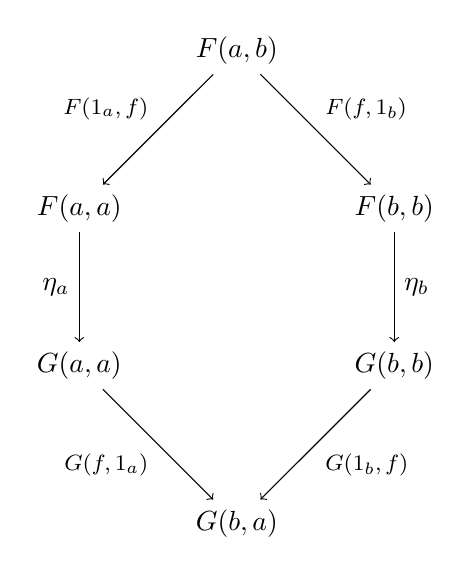
\begin{tikzpicture}
				\node (ab) at (0, 6) {$F(a, b)$};
				\node (F1) at (-2, 4) {$F(a, a)$};
				\node (F2) at (2, 4) {$F(b, b)$};
				\node (G1) at (-2, 2) {$G(a, a)$};
				\node (G2) at (2, 2) {$G(b, b)$};
				\node (ba) at (0, 0) {$G(b, a)$};
				
				\draw[->] (ab) edge node[above left]{\footnotesize$F(\mathbbm{1}_a, f)$} (F1) (F1) edge node[left]{$\eta_a$} (G1) (G1) edge node[below left]{\footnotesize$G(f, \mathbbm{1}_a)$} (ba);
				\draw[->] (ab) edge node[above right]{\footnotesize$F(f, \mathbbm{1}_b)$} (F2) (F2) edge node[right]{$\eta_b$} (G2) (G2) edge node[below right]{\footnotesize$G(\mathbbm{1}_b, f)$} (ba);
			\end{tikzpicture}
			\caption{Dinatural transformation.}
			\label{fig:dinatural}
		\end{figure}
	}
	
\subsection{Adjunctions}

	\newdef{Hom-set adjunction}{\index{adjunction}
		Let $\func{F}{C}{D}$ and $\func{G}{D}{C}$ be two functors. These functors form a hom-set adjunction (often just called an adjunction) if the following isomorphism is natural in $a, b$:
		\begin{gather}
			\text{hom}_D(Fa, b)\cong\text{hom}_C(a, Gb)
		\end{gather}
		The functor $F$ (resp. G) is called the left (resp. right) adjoint\footnote{Sometimes the word \textbf{adjunct} is used (French versus Latin).}.
	}
	\begin{notation}
		An adjunction$(F, G)$ between categories $\mathbf{C}, \mathbf{D}$ is often denoted by: \[\textbf{C}\adj{F}{G}\textbf{D}\] or if the ambient categories are clear by: \[F\dashv G\]
	\end{notation}
	
	\newdef{Unit-counit adjunction}{\index{triangle!identities}\index{unit}\index{zig-zag|see{triangle identity}}
		Let $\func{F}{C}{D}$ and $\func{G}{D}{C}$ be two functors. These functors form a unit-counit adjunction if there exist natural transformations
		\begin{align}
			\varepsilon: F\circ G\Rightarrow 1_D\\
			\eta: 1_C\Rightarrow G\circ F
		\end{align}
		such that the following compositions are identity morphisms:
		\begin{align}
			F\xrightarrow{F\eta}FGF\xrightarrow{\varepsilon F}F\\
			G\xrightarrow{\eta G}GFG\xrightarrow{G\varepsilon}G
		\end{align}
		These identities are sometimes called the \textbf{triangle identities} or \textbf{zig-zag identities} (the latter results from the shape of the associated string diagram). The transformations $\varepsilon$ and $\eta$ are called the \textbf{unit} and \textbf{counit} respectively.
	}
	
	\begin{property}
		Every hom-set adjuction induces a unit-counit adjunction. Let $\Phi_{a, b}$ be the natural isomorphism associated to the hom-set adjunction $F\dashv G$. The unit $\varepsilon_d$ is obtained as the adjunct $\Phi^{-1}_{Gd, d}(1_{Gd})$ of the identity morphism on $Gd\in\ob{C}$ and the counit $\eta_c$ is analogously defined as the adjunct $\Phi_{c, Fc}(1_{Fc})$ of the identity morphism at $Fc\in\ob{D}$.
		
		Similarly every unit-counit adjunction induces a hom-set adjunction. Consider a morphism $f:Fc\rightarrow d$. The (right) adjunct $\tilde{f}$ is defined as the composition \[Gf\circ\eta_c:c\rightarrow (G\circ F)c\rightarrow Gd\] Similarly, consider a morphism $\tilde{g}:c\rightarrow Gd$. The (left) adjunct $g$ is defined as the composition \[\varepsilon_d\circ F\tilde{g}: Fc\rightarrow (F\circ G)d\rightarrow d\]
	\end{property}

	Now it should be obvious that the above definition of a unit-counit adjunction can be generalized to general 2-categories:
	\newdef{Adjunction in 2-category}{\index{adjunction}
		Let \textbf{C} be a 2-category. An adjunction in \textbf{C} is a pair of 1-morphisms $F:a\rightarrow b$ and $G:b\rightarrow a$ together with 2-morphisms $\varepsilon:F\circ G\Rightarrow 1_b$ and $\eta:1_a\Rightarrow G\circ F$ that satisfy the zig-zag identities.
	}
	
	\begin{remark}[Duals and adjunctions]
		If one looks at the defining relations of duals in a rigid monoidal category one should see that these are in fact the same as the defining relations of the unit and counit of an adjunction. This is a consequence of the fact that a 2-category with a single object can be regarded as a (strict) monoidal category where the composition in the 2-category becomes the tensor product in the monoidal category. Similarly adjoint 1-morphisms in the 2-category become duals in the monoidal category.
	\end{remark}

\subsection{Constructions}

	\newdef{Discrete fibration}{\index{fibration}
		Let $\func{F}{A}{B}$ be a functor. $F$ is a discrete fibration if for every object $A\in\ob{A}$ and every morphism $f:B\rightarrow FA$ in $\textbf{B}$ there exists a unique morphism $g:C\rightarrow A$ in $\textbf{A}$ such that $F(g) = f$, where $B\in\ob{B}, C\in\ob{A}$.
	}

	\newdef{Dagger category\footnotemark}{\index{category!dagger}\index{involution}\label{cat:dagger_category}
		\footnotetext{Also called a \textbf{$\dag$-category}.}
		A category equipped with a contravariant endofunctor, i.e. a functor $\dag:\textbf{C}^{op}\rightarrow\textbf{C}$, such that:
		\begin{enumerate}
			\item $\forall C\in\ob{C}: \mathbbm{1}_C^\dag = \mathbbm{1}_C$
			\item $\dag\circ\dag = \mathbbm{1}_C$
		\end{enumerate}
		The second property says that $\dag$ is an \textbf{involutive} functor.
	}
	\remark{The concept of a dagger structure allows the usual definition of \textbf{unitary} and \textbf{self-adjoint} morphisms.}\index{unitary}
	\begin{property}
		The unitary morphisms in a dagger category form a groupoid\footnote{See definition \ref{cat:groupoid}.}.
	\end{property}
	
	\newdef{Comma category}{\index{category!comma}
		Let $\textbf{A}, \textbf{B}$ and $\textbf{C}$ be three categories and let $\func{F}{A}{C}$ and $\func{G}{B}{C}$ be two functors. The comma category $F\downarrow G$ is defined as follows:
		\begin{itemize}
			\item Objects are triples $(A, B, \gamma)$ where $A\in\ob{A}, B\in\ob{B}$ and $\gamma:FA\rightarrow GB\in\text{hom}(\textbf{C})$.
			\item Morphisms $(A, B, \gamma)\rightarrow(K, L, \sigma)$ are pairs $(f, g)$ where $f:A\rightarrow K\in\text{hom}(\textbf{A})$ and $g:B\rightarrow L\in\text{hom}(\textbf{B})$ such that $\sigma\circ F(f) = G(g)\circ\gamma$.
			\item Composition of morphisms is defined componentwise.
		\end{itemize}
	}
	\newdef{Slice category}{\index{category!slice}
		Let \textbf{C} be a category and let $c\in\ob{C}$. The slice category $\textbf{C}/c$ of $\textbf{C}$ over $c$ is defined as follows:
		\begin{itemize}
			\item The objects are morphisms in $\textbf{C}$ with codomain $c$.
			\item The morphisms $f\rightarrow g$ are morphisms $h$ in $\textbf{C}$ such that $g\circ h = f$.
		\end{itemize}
	}
	
\subsection{Monads}

	\newdef{Monad}{\index{monad}
		A monad is a triple $(T, \mu, \eta)$ where $\func{T}{C}{C}$ is an endofunctor and $\mu:T^2\rightarrow T, \eta:\text{id}_{\mathbf{C}}\rightarrow T$ are natural transformations satisfying the following (coherence) conditions:
		\begin{enumerate}
			\item As natural transformation from $T^3$ to $T$ we have:
			\begin{gather}
				\mu\circ T\mu = \mu\circ\mu_T
			\end{gather}
			\item As natural transformation from $T$ to itself we have:
			\begin{gather}
				\mu\circ T\eta = \mu\circ\eta_T = \mathbbm{1}
			\end{gather}
		\end{enumerate}
		These conditions say that a monad is a monoid in the category $\mathbf{End}_{\mathbf{C}}$ of endofunctors on $\mathbf{C}$.
	}
	\begin{example}[Adjunction]
		Every adjunction $F\dashv G$, with unit $\varepsilon$ and counit $\eta$, induces a monad of the form $(GF, G\varepsilon F, \eta)$.
	\end{example}
	
	\newdef{Algebra\footnotemark\ over a monad}{\index{algebra!over a monad}
		\footnotetext{A more suitable name would be ''module over a monad'', since these are modules over a monoid if we view monads as monoids in $\mathbf{End}_{\mathbf{C}}$.}
		Consider a monad $(T, \mu, \eta)$ on a category $\mathbf{C}$. A algebra over $T$ is a couple $(a, \kappa)$ where $a\in\ob{C}$ and $\kappa:Ta\rightarrow a$ such that the following conditions are satisfied:
		\begin{enumerate}
			\item $\kappa\circ T\kappa = \kappa\circ\mu_a$
			\item $\kappa\circ\eta_a = \mathbbm{1}_a$
		\end{enumerate}
		Morphisms $(a, \kappa_a)\rightarrow(b, \kappa_b)$ of $T$-algebras are morphisms $f:a\rightarrow b$ in $\mathbf{C}$ such that $f\circ\kappa_a = \kappa_b\circ Tf$.
	}
	\newdef{Eilenberg-Moore category}{\index{Eilenberg-Moore}
		Given a monad $T$ over a category $\mathbf{C}$ we define the Eilenberg-Moore category $\mathbf{C}^T$ as the category of $T$-algebras.
	}
	
	\newdef{Monadic adjunction}{
		An adjunction between categories $\mathbf{C}$ and $\mathbf{D}$ is said to be monadic if there exists an equivalence between $D$ and the Eilenberg-Moore category of the induced monad.
	}
	\newdef{Monadic functor}{\index{functor!monadic}
		A functor is said to be monadic if it admits a left adjoint such that the adjunction is monadic.
	}
	
	\begin{theorem}[Beck's monadicity theorem]
		Consider a functor $\func{F}{C}{D}$. This functor is monadic if and only if the following conditions are satisfied:
		\begin{itemize}
			\item $F$ admits a left adjoint.
			\item $F$ reflects isomorphisms.
			\item $\mathbf{C}$ has all coequalizers of $F$-split parallel pairs\footnote{These are parallel pairs $f,g$ such that the image $Ff, Fg$ under $F$ admits a split coequalizer.} and $F$ preserves these coequalizers.
		\end{itemize}
	\end{theorem}
	\remark{A sufficient condition for monadicity is obtained by replacing the third item above by the following weaker statement: ''$\mathbf{C}$ has all coequalizers of reflexive pairs and $F$ preserves these coequalizers.'' This weaker form is called the \textbf{crude monadicity theorem}.}

	\newdef{Closure operator\footnotemark}{\label{cat:closure_operator}\index{closure!operator}\index{modal operator|see{closure operator}}
		\footnotetext{Also called a \textbf{modal operator}.}
		Consider a monad $\func{T}{C}{C}$ with unit and product maps $\eta, \mu$. This monad is called a closure operator if the product map is a natural isomorphism.
		
		Given a closure operator $\func{T}{C}{C}$, one calls the object $Tx$ the closure of $x\in\ob{C}$. The \textbf{closing map} of an object $x\in\ob{C}$ is defined as the morphism $\eta_x$ and $x$ is said to be $T$\textbf{-closed} exactly if its closing map is an isomorphism.
	}

\section{Initial and terminal objects}

	\newdef{Initial object}{
		An object $O$ in a category $\textbf{C}$ is called initial if for every other object $P$ there exists a unique morphism $\iota_P:O\rightarrow P$.
	}
	\newdef{Terminal object}{
		An object $O$ in a category $\textbf{C}$ is called terminal if for every other object $P$ there exists a unique morphism $\tau_P:P\rightarrow O$. This object is sometimes denoted by $\mathbf{1}$.
	}
	\begin{property}
		If an initial (resp. terminal) object exists, then it is unique (possibly up to isomorphism).
	\end{property}
	\newdef{Well-pointed category}{
		A category is said to be well-pointed if the terminal object is a generator\footnote{See definition \ref{cat:generator}.}.
	}
	
	\newdef{Zero object}{\index{zero!object}\label{cat:zero_object}
		An object which is both initial and terminal. The zero object is often denoted by $\mathbf{0}$.
	}
	\begin{property}[Zero morphism]
		From the definition of the zero object it follows that for any two objects $A, B$ there exists a unique morphism $0_{AB}:A\rightarrow0\rightarrow B$.
	\end{property}
	\newdef{Pointed category}{\index{pointed!category}
		A category is said to be pointed if it contains a zero object.
	}
	
	\newdef{Global element}{\index{global!element}\label{category:global_element}
		Let $\textbf{C}$ be a category with terminal object $\mathbf{1}$. A global element of an object $X\in\ob{C}$ is a morphism $\mathbf{1}\rightarrow X$.
	}
	\begin{remark}
		In the category \textbf{Set} the elements of a set $S$ are in one-to-one correspondence with the global elements of $S$ and one has the important property (axiom) that two functions $f, g:S\rightarrow S'$ coincide if their evaluation at every element $s\in S$ is equal or equivalently if the precompositions with global elements coincide.
		
		However this way of checking equality can fail in other categories. Consider for example \textbf{Grp}. In this category the terminal object is $0 = \{e\}$. The only morphism from this group to any other group $G$ is the one mapping $e$ to the unit in $G$ ($0$ is also an initial object in \textbf{Grp}). It is obvious that precomposition with this morphism tells us nothing about the equality of other morphisms. To recover the technique used in \textbf{Set} one needs to generalize the notion of "element":
	\end{remark}
	\newdef{Generalized element}{\index{shape}
		Let $\textbf{C}$ be category and consider an object $X$ in $\textbf{C}$. For any object $Y\in\ob{C}$ one calls a morphism $Y\rightarrow X$ a generalized element of $X$. The morphisms $Y\rightarrow X$ are also called $\textbf{Y-elements}$ in $X$ or elements of \textbf{shape} $Y$ in $X$.
	}

\section{Diagrams and universal constructions}

	\newdef{Diagram}{\index{diagram}
		A diagram in $\textbf{C}$ with index category $\textbf{I}$ is a (covariant) functor $\func{D}{I}{C}$.
	}
	
	\newdef{Cone}{\index{cone}
		Let $\func{D}{I}{C}$ be a diagram. A cone from $a\in\ob{C}$ to $D$ consists of a family of morphisms $\psi_i:a\rightarrow Di, \forall i\in\ob{I}$ such that $\psi_j = Df\circ\psi_i$ for all morphisms $f:i\rightarrow j\in\text{hom}(\textbf{I})$, as depicted in figure \ref{fig:cone_component}.
		
		\begin{figure}[ht!]
			\centering
			\begin{subfigure}[b]{0.49\textwidth}
				\centering
				\begin{tikzpicture}
					\matrix (m) [matrix of math nodes,row sep=3em,column sep=3em, minimum width=1em, ampersand replacement=\&]{
						\&a\&\\
						Di\vphantom{(}\&\&Df(i)\\
					};
					\draw[->] (m-1-2) -- (m-2-1) node[pos=0.5, above left]{$\psi_i$};
					\draw[->] (m-1-2) -- (m-2-3) node[pos=0.5, above right]{$\psi_{f(i)}$};
					\draw[->] (m-2-1) -- (m-2-3) node[pos=0.5, below]{$Df$};
				\end{tikzpicture}
				\caption{Component of cone over $D$.}
				\label{fig:cone_component}
			\end{subfigure}
			\begin{subfigure}[b]{0.49\textwidth}
				\centering
				\begin{tikzpicture}
					\matrix (m) [matrix of math nodes,row sep=3em,column sep=3em, minimum width=1em, ampersand replacement=\&]{
						a\vphantom{b}\&\&b\\
						\&Di\&\\
					};
					\draw[->] (m-1-1) -- (m-2-2) node[pos=0.5, below left]{$\psi_i$};
					\draw[->] (m-1-3) -- (m-2-2) node[pos=0.5, below right]{$\phi_i$};
					\draw[->] (m-1-1) -- (m-1-3) node[pos=0.5, above]{$f$};
				\end{tikzpicture}
				\caption{Morphism of cones.}
				\label{fig:cone_morphism}
			\end{subfigure}
			\label{fig:cone}
		\end{figure}
	}
	\begin{adefinition}\index{diagonal!functor}
		This definition can be reformulated by defining an additional functor\footnote{The notation $\Delta_a$ tells us that $\Delta:C\rightarrow [\textbf{I},\textbf{C}]$ is the \textbf{diagonal functor}, i.e. $\Delta_c\equiv\Delta(c)$ is the constant functor from $\textbf{I}$ to $\textbf{C}$ with target object $c$.} $\Delta_a:\textbf{I}\rightarrow\textbf{C}$ which maps every element $i\in\ob{I}$ to $a$ and every morphism $g\in\text{hom}(\textbf{I})$ to id$_a$. The morphisms $\psi_c$ can then be seen as the components of a natural transformation $\psi:\Delta_a\Rightarrow D$. Hence a cone $(a, \psi)$ is an element of $[\textbf{I}, \textbf{C}](\Delta_a, D)$.
	\end{adefinition}

	\newdef{Morphism of cones}{\index{morphism!of cones}
		Let $\func{D}{I}{C}$ be a diagram and let $(a, \psi), (b, \phi)$ be cones to $D$. A morphism between these cones is a morphism of the apexes $f:a\rightarrow b$ such that the diagrams of the form \ref{fig:cone_morphism} commute for all $i\in\ob{I}$. The cones to $D$ together with these morphisms form a category $\textbf{Cone}(D)$, in fact this can easily be seen to be the comma category $(\Delta \downarrow D)$.
	}
	
	\newdef{Limit}{\index{limit}
		Consider a diagram $\func{D}{I}{C}$. The limit $\lim D$ of this diagram, if it exists, is the terminal object of the category $\textbf{Cone}(D)$.
	}
	This definition gives us the following universal property:
	\begin{uproperty}
		Let $\func{D}{I}{C}$ be a diagram and let $\lim D$ be its limit. For every cone $(a, \psi)\in\textbf{Cone}(D)$ there exists a unique morphism $f:c\rightarrow\lim D$.
	\end{uproperty}
	
	\begin{example}[Terminal object]
		A terminal object $\mathbf{1}$ is a limit over the empty diagram.
	\end{example}
	
	\newdef{Equalizer}{\index{equalizer}\index{fork}
		Consider the following diagram:\[X\overset{f}{\underset{g}{\rightrightarrows}} Y\] The limit of this diagram is called the equalizer of $f$ and $g$. Explicitly the equalizer is the universal object $E$ together with a morphism $e: E\rightarrow X$ such that $f\circ e = g\circ e$.
	}
	\newdef{Split coequalizer}{
		First we define a \textbf{cofork} diagram, i.e. a diagram \[a\overset{f}{\underset{g}{\rightrightarrows}} b\overset{t}{\rightarrow} c\] where $t\circ f = t\circ g$. A split coequalizer\footnote{A coequalizer, as obtained by dualizing the previous definition, is just a universal cofork.} is a cofork together with a section of $\varphi$ of $f$ and a section $\sigma$ of $t$ such that $\sigma\circ t = g\circ \varphi$.
	}
	
	\newdef{Finitely complete category}{\index{finitely!complete}
		A category is said to be finitely complete if it has a terminal object and if all binary equalizers and products exist.
	}
	\newadef{Finitely complete category}{
		A category is said to be finitely complete if all finite limits exist.
	}
	
	\newdef{Span}{\index{span}
		A span in a category $C$ is a diagram of the form \ref{fig:cat_span}.
		
		Let $\Lambda$ be the category with three objects $\{-1, 0, 1\}$ and two morphisms $i:0\rightarrow -1$ and $j:0\rightarrow 1$. By the above definition of a diagram a span in $C$ is equivalent to a functor $\func{S}{\Lambda}{C}$.
	}
	
	\newdef{Pullback\footnotemark}{\index{pullback}\label{cat:pullback}
		\footnotetext{Also called a \textbf{fibre product} or \textbf{Cartesian square}.}
		The pullback of two morphisms $f:A\rightarrow C$ and $g:B\rightarrow C$ is defined as the limit of cospan \ref{fig:pullback}.
	}
	\begin{figure}[!ht]
		\centering
		\begin{subfigure}[b]{0.49\textwidth}
			\centering
			\begin{tikzpicture}
				\matrix (m) [matrix of math nodes,row sep=2em,column sep=2em, minimum width=1em, ampersand replacement=\&]{
					\&S\&\\
					A\&\&B\\
				};
				\draw[->] (m-1-2) -- (m-2-1) node[pos=0.5, above left]{$f$};
				\draw[->] (m-1-2) -- (m-2-3) node[pos=0.5, above right]{$g$};
			\end{tikzpicture}
			\caption{Span (category theory).}
			\label{fig:cat_span}
		\end{subfigure}
		\begin{subfigure}[b]{0.49\textwidth}
			\centering
			\begin{tikzpicture}
				\matrix (m) [matrix of math nodes,row sep=2em,column sep=2em, minimum width=1em, ampersand replacement=\&]{
					A\&\&B\\
					\&C\&\\
				};
				\draw[->] (m-1-1) -- (m-2-2) node[pos=0.5, below left]{$f$};
				\draw[->] (m-1-3) -- (m-2-2) node[pos=0.5, below right]{$g$};
			\end{tikzpicture}
			\caption{Cospan.}
			\label{fig:pullback}
		\end{subfigure}
		\caption{}
	\end{figure}
	
	\begin{notation}[Pullback]
		The pullback of two morphisms $f:A\rightarrow C$ and $g:B\rightarrow C$ is often denoted by $A\times_C B$.
	\end{notation}
	
	\begin{property}
		If a terminal object $\mathbf{1}$ exists then the pullback $A\times_{\mathbf{1}}B$ is equal to the (Cartesian) product  $A\times B$.
	\end{property}
	\newdef{Pushout}{\index{pushout}
		The dual notion of a pullback, i.e. the colimit of a span.
	}

	\newdef{Wedge}{\index{wedge}
		Consider a profunctor $F:\mathbf{C}^{op}\times\mathbf{C}\rightarrow\mathbf{Set}$. A wedge $e:w\rightarrow F$ is an object $w\in\ob{Set}$ together with a collection of morphisms $e_c:w\rightarrow F(c, c)$ indexed by $\ob{C}$ such that for any morphism $f:c\rightarrow c'$ the following diagram commutes:
		\begin{gather*}
			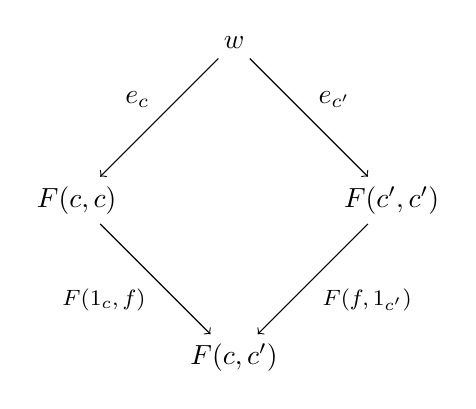
\begin{tikzpicture}
				\node (W) at (0, 4) {$w$};
				\node (F1) at (-2, 2) {$F(c, c)$};
				\node (F2) at (2, 2) {$F(c', c')$};
				\node (F) at (0, 0) {$F(c, c')$};
				\draw[->] (W) edge node[above left]{$e_c$} (F1) (F1) edge node[below left]{\footnotesize$F(\mathbbm{1}_c, f)$} (F);
				\draw[->] (W) edge node[above right]{$e_{c'}$} (F2) (F2) edge node[below right]{\footnotesize$F(f, \mathbbm{1}_{c'})$} (F);
			\end{tikzpicture}
		\end{gather*}
		As was the case for cones, one can reformulate this in terms of (di)natural transformations. A wedge $(w, e)$ of a profunctor $F:\mathbf{C}^{op}\times\mathbf{C}\rightarrow\mathbf{Set}$ is a dinatural transformation from the constant profunctor $\Delta_w$ to $F$.
	}
	\newdef{End}{\index{end}
		The end of a profunctor $F:\mathbf{C}^{op}\times\mathbf{C}\rightarrow\mathbf{Set}$ is defined as the universal wedge of $F$. The components of the wedge are called the \textbf{projection maps} of the end. This stems from the fact that for a discrete category the end coincides with the product $\prod_{c\in\ob{C}}F(c, c)$.
	}
	\newnot{End}{
		The end of a profunctor $F:\mathbf{C}^{op}\times\mathbf{C}\rightarrow\mathbf{Set}$ is often denoted using an integral sign with subscript: \[\int_{c\in\mathbf{C}}F(c, c)\] For the dual construction, i.e. a \textbf{coend}, one uses the integral sign with superscript.
	}
	\begin{example}[Natural transformations]
		Consider two functors $\func{F, G}{C}{D}$. The map $(c, c')\mapsto\mathbf{D}(Fc, Gc')$ gives a profunctor $H:\mathbf{C}^{op}\times\mathbf{C}\rightarrow\mathbf{Set}$. If we look at the wedge condition for this profunctor (especially the lower half) we get the following equality for all morphisms $f:c\rightarrow c'$:
		\begin{gather}
			\tau_{c'}\circ Ff = Gf\circ \tau_c
		\end{gather}
		where $\tau_c$ is the projection of the wedge associated to the object $c\in\ob{C}$. Comparing this equality to definition \ref{cat:natural} we immediately see that the end $\int_{c\in\mathbf{C}}\mathbf{D}(Fc, Gc)$ is exactly Nat$(F, G)$.
	\end{example}
	
	\begin{property}
		The following equality can be used to turn ends into coends and vice versa:
		\begin{gather}
			\mathbf{Set}\left(\int^{c\in\mathbf{C}}F(c, c), c'\right) = \int_{c\in\mathbf{C}}\mathbf{Set}\left(F(c, c), c'\right)
		\end{gather}
	\end{property}
	
	Using the above properties and definitions one obtains the following Yoneda-like statements:
	\begin{theorem}[Ninja Yoneda lemma]\index{Yoneda!lemma}
		Let $\func{F}{C}{D}$ be a covariant functor. The following two isomorphisms follow from the ordinary Yoneda lemma:
		\begin{gather}
			\int_{c'\in\mathbf{C}}\mathbf{Set}\left(\mathbf{C}(c, c'), Fc'\right)\cong Fc
		\end{gather}
		\begin{gather}
			\int^{c\in\mathbf{C}}\mathbf{C}(c, c')\times Fc\cong Fc'
		\end{gather}
	\end{theorem}
	
	\newdef{Kan extension}{\index{Kan!extension}
		Consider two functors $\func{F}{C}{D}$ and $\func{G}{C}{E}$ and denote the terminal category by $\mathbf{1}$. The right Kan extension\footnote{The left Kan extension Lan$_GF$ is obtained by dualizing this construction.} of $F$ along $G$ is given by the universal functor $\func{\text{Ran}_GF}{E}{D}$ and natural transformation $\eta:\text{Ran}_GF\circ G\Rightarrow F$:
		\begin{gather*}
			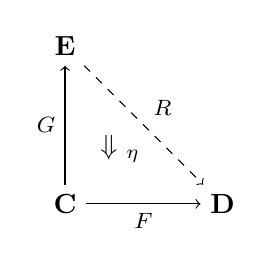
\begin{tikzpicture}
				\node (E) at (0, 2) {$\mathbf{E}$};
				\node (C) at (0, 0) {$\mathbf{C}$};
				\node (D) at (2, 0) {$\mathbf{D}$};
				\node (A) at (0.7, 0.7) {$\Downarrow_{\ \eta}$};
				\draw[->] (C) -- node[left]{\footnotesize$G$} (E);
				\draw[->] (C) -- node[below]{\footnotesize$F$} (D);
				\draw[dashed, ->] (E) -- node[above right]{\footnotesize$R$} (D);
			\end{tikzpicture}
		\end{gather*}
		Universality means that every other natural transformation $\chi:H\circ G\Rightarrow F$ factors uniquely through $\eta$.
	}
	\begin{example}[Limit]
		By choosing the functor $G$ in the definition of a right Kan extension to be the unique functor $!_C:\mathbf{C}\rightarrow\mathbf{1}$ into the terminal category one obtains the definition of a limit, i.e. $\lim F = \text{Ran}_{!_C}F$. Similarly one can obtain the colimit as the left Kan extension.
	\end{example}
	
	\newdef{Absolute Kan extension}{
		A (left) Kan extension Lan$_GF$ is said to be absolute if for every functor $H$ with the same codomain as $F$ the following isomorphism holds:
		\begin{gather}
			H(\text{Lan}_GF)\cong\text{Lan}_G(HF)
		\end{gather}
		There exists an analogous definition for right Kan extensions.
	}

	\newadef{Kan extension}{
		The construction above gives a functor Ran$_G$ from the functor category $[\mathbf{C}, \mathbf{D}]$ to the functor category $[\mathbf{E}, \mathbf{D}]$. The right Kan extension Ran$_G$ can be defined as the right adjoint to the pullback functor $G^*:F\mapsto F\circ G$. Similarly one can define the left Kan extension as the left adjoint to the pullback functor $G^*$.
	}
	\remark{Using this equivalence of hom-spaces one can generalize the Kan extension from $\mathbf{Cat}$ to any 2-category.}
	
	The existence of Kan extensions can also be used to determine the existence of adjoints:
	\begin{property}
		A functor $\func{F}{C}{D}$ admits a left adjoint\footnote{An analogous statement holds for right adjoints.} if and only if the right Kan extension of the identity functor $\func{\mathbbm{1}}{C}{C}$ along $F$ exists. If it exists and if it is an absolute extension then the left adjoint is given exactly by this Kan extension.
	\end{property}
	
\section{Morphisms}

	\newdef{Section}{\index{section}
		A section of a morphism $f:a\rightarrow b$ is a right-inverse, i.e. a morphism $g:b\rightarrow a$ such that $f\circ g=\mathbbm{1}_b$.
	}
	\newdef{Monomorphism}{\index{monomorphism}
		Let \textbf{C} be a category. A morphism $\mu\in\textbf{C}(A, B)$ is called a mono\footnote{Sometimes just a \textbf{mono} or a \textbf{monic} morphism.} if for every object $X\in\ob{C}$ and every two morphisms $\alpha_1, \alpha_2\in\textbf{C}(X, A)$ such that $\mu\circ\alpha_1 = \mu\circ\alpha_2$ we can conclude that $\alpha_1=\alpha_2$.
	}
	\newdef{Epimorphism}{\index{epimorphism}
		Let \textbf{C} be a category. A morphism $\varepsilon\in\textbf{C}(A, B)$ is called an epimorphism\footnote{Sometimes just an \textbf{epi} or an \textbf{epic} morphism.} if for every object $X\in\ob{C}$ and every two morphisms $\alpha_1, \alpha_2\in\textbf{C}(B, X)$ such that $\alpha_1\circ\varepsilon = \alpha_2\circ\varepsilon$ we can conclude that $\alpha_1=\alpha_2$.
	}
	
	\newdef{Balanced category}{\index{category!balanced}\label{category:balanced}
		A category is said to be balanced if every monic epi is an isomorphism.
	}
	
	\begin{property}[Global elements]
		Every global element\footnote{See definition \ref{category:global_element}.} is monic.
	\end{property}
	
	\newdef{Reflexive pair}{
		Two parallel morphisms $f, g:a\rightarrow b$ are said to form a reflexive pair if they have a common section, i.e. there exists a morphism $\sigma:b\rightarrow a$ such that $f\circ\sigma=g\circ\sigma$.
	}
	
	\begin{property}[Equalizing morphism]
		Consider an equalizer $(E, e)$. The equalizing morphism $e$ is monic. Similarly a coequalizing morphism is epic.
	\end{property}

	\newdef{Regular monomorphism}{\index{regular!morphism}
		A mono is said to be regular if it arises as an equalizer of two parallel morphisms.
	}
	\begin{property}[Regular bimorphism]\label{category:regular_iso}
		A monic regular epimorphism is an isomorphism. Analogously so is an epic regular monomorphism is an isomorphism.
	\end{property}
	
	\newdef{Injective object}{\index{injective!object}
		Let \textbf{C} be an category. An object $I\in\ob{C}$ is said to be injective if for every $A, B\in\ob{C}$, mono $f:A\rightarrow B$ and morphism $g:A\rightarrow I$ there exists a morphism $\phi:B\rightarrow I$ such that $\phi\circ f = g$.
		\begin{figure}[ht!]
			\centering
			\begin{subfigure}[b]{0.49\textwidth}
				\centering
				\begin{tikzpicture}
					\matrix (m) [matrix of math nodes,row sep=7em,column sep=7em, minimum width=2em, ampersand replacement=\&]{
						A\&B\\
						I\&\\
					};
					\draw[right hook ->] (m-1-1) -- (m-1-2) node[pos=0.5, above]{$f$};
					\draw[->] (m-1-1) -- (m-2-1) node[pos=0.5, left]{$g$};
					\draw[dashed, ->] (m-1-2) -- (m-2-1) node[pos=0.5, below right]{$\phi$};
				\end{tikzpicture}
				\caption{Injective object $I$.}
				\label{fig:injective_object}
			\end{subfigure}
			\begin{subfigure}[b]{0.49\textwidth}
				\centering
				\begin{tikzpicture}
					\matrix (m) [matrix of math nodes,row sep=7em,column sep=7em, minimum width=2em, ampersand replacement=\&]{
						A\&B\\
						\&P\\
					};
					\draw[->>] (m-1-1) -- (m-1-2) node[pos=0.5, above]{$f$};
					\draw[->] (m-2-2) -- (m-1-2) node[pos=0.5, right]{$g$};
					\draw[dashed, ->] (m-2-2) -- (m-1-1) node[pos=0.5, below left]{$\phi$};
				\end{tikzpicture}
				\caption{Projective object $P$.}
				\label{fig:projective_object}
			\end{subfigure}
		\end{figure}
	}
	
	Dually one can construct:
	\newdef{Projective object}{\index{projective!object}
		Let \textbf{C} be an category. An object $P\in\ob{C}$ is said to be projective if for every $A, B\in\ob{C}$, epi $f:A\rightarrow B$ and morphism $g:P\rightarrow A$ there exists a morphism $\phi:P\rightarrow B$ such that $f\circ\phi = g$.
	}
	
	\newdef{Subobject}{\index{subobject}
		Let \textbf{C} be a category and let $A\in\ob{C}$ be any object. A subobject $B$ of $A$ is a mono $B\hookrightarrow A$.
		
		In fact one should work up to isomorphism and hence the complete definition goes as follows. A subobject $B$ of $A$ in the category \textbf{C} is an isomorphism class of monos $i:B\hookrightarrow A$ in the slice category $\textbf{C}/A$.
	}
	\newdef{Well-powered category}{\index{category!well-powered}
		A category \textbf{C} is said to be well-powered if for every object $A\in\ob{C}$ the class of subobjects \textbf{Sub}$(A)$ is small.
	}
	
	\newdef{Generator\footnotemark}{\index{generator}\label{cat:generator}
		\footnotetext{Also called a \textbf{separator}.}
		Let \textbf{C} be a category. A collection of objects $\{O_i\in\ob{C}\}$ is called a collection of generators for \textbf{C} if, given any two objects $A, B\in\ob{C}$ and any two morphisms $f, g:A\rightarrow B$, we have that $f\neq g\implies\exists j\in I, h_j\in\textbf{C}(O_i, A): f\circ h_j\neq g\circ h_j$.
	}
	
	\newdef{Decategorification}{
		Let \textbf{C} be a (essentially) small category. The set of isomorphism classes of \textbf{C} is called the decategorification of \textbf{C}. This is given by a functor \[K:\textbf{Cat}\rightarrow\textbf{Set}\]
	}
	
	\newdef{Lift}{\index{lift}
		A lift of a morphism $f:A\rightarrow B$ along an epi $e:X\rightarrow B$ is a morphisms $\tilde{f}:A\rightarrow X$ satisfying $f = e\circ\tilde{f}$.
	}
	\newdef{Lifting property}{\index{orthogonal}
		A morphism $f:A\rightarrow B$ has the left lifting property with respect to a morphism $g:C\rightarrow D$ if for every commutative diagram
		\begin{figure}[ht!]
			\centering
			\begin{tikzcd}[ampersand replacement=\&, row sep=4em,column sep=4em, minimum width=2em]
				A \arrow[r] \arrow[d, "f"'] \& C \arrow[d, "g"]\\
				B \arrow[ur, "\psi"] \arrow[r] \& D
			\end{tikzcd}
			\caption{Left lifting property.}
			\label{fig:lifting_property}
		\end{figure}
		there exists a morphism $\psi:B\rightarrow C$ such that the triangles commute. The morphism $g$ is also said to have the right lifting property with respect to $f$. If the morphism $\psi$ is unique then $f$ and $g$ are said to be \textbf{orthogonal}.
	}
	
	\newdef{Weak factorization system}{\index{weak!factorization}\label{category:wfc}
		Consider a category \textbf{C}. A pair $(L, R)$ of classes of morphisms in \textbf{C} is called a weak factorization system (WFS) if it satisfies the folllowing 3 properties:
		\begin{enumerate}
			\item Every morphism in \textbf{C} factors as a composition $g\circ f$ where $f\in L$ and $g\in R$.
			\item $L$ consists of the morphisms in \textbf{C} that have the left lifting property with respect to morphisms in $R$.
			\item $R$ consists of the morphisms in \textbf{C} that have the right lifting property with respect to morphisms in $L$.
		\end{enumerate}
	}
	
	\newdef{Localization}{\index{localization}\label{cat:localization}
		Consider a category \textbf{C} with a collection of morphism $M\subset\text{mor}(\textbf{C})$. The localization of \textbf{C} with respect to $M$ is constructed by adding for each morphism $f\in M$ a formal inverse to $\text{mor}(\textbf{C})$.
	}

\section{Abelian categories}

	\newdef{Pre-additive category}{
		A (locally small) category enriched over \textbf{Ab}, i.e. every hom-set is an Abelian group and composition is bilinear.
	}
	\newdef{$k$-linear category}{\index{category!linear}
		Let \textbf{Vect}$_k$ denote the category of vector spaces over the base field $k$. A $k$-linear category is a category enriched over \textbf{Vect}$_k$.
	}
	
	\begin{property}\index{zero!object}
		Let \textbf{A} be a pre-additive category and let $X\in\ob{A}$. The following statements are equivalent:
		\begin{itemize}
			\item $X$ is an initial object.
			\item $X$ is a final object.
			\item $\mathbbm{1}_X$ = 0
		\end{itemize}
		Any initial/terminal object is hence a zero object\footnote{See definition \ref{cat:zero_object}.}.
	\end{property}
	\begin{property}\index{biproduct}
		In a pre-additive category the finite products $\prod_{i\in I}X_i$ are isomorphic to the finite coproducts $\bigsqcup_{i\in I} X_i$ (which are called \textbf{direct sums} in this context). If a product $X\times Y$ exists then so does the coproduct $X\sqcup Y$ and if the coproduct exists then so does the product. In general if a product and coproduct exist and are equal then one speaks of a \textbf{biproduct}.
	\end{property}
	
	\newdef{Additive category}{\index{additive!category}
		A pre-additive category in which all finite biproducts exist.
	}
	
	If one speaks of additive categories, one generally assumes that the associated functors are of a specific type:
	\newdef{Additive functor}{\index{additive!functor}\label{additive_functor}
		Let $\mathbf{A}, \mathbf{A'}$ be additive categories. A functor $\func{F}{A}{A'}$ is said to be additive if it preserves all biproducts, i.e. if it satisfies the following conditions:
		\begin{itemize}
			\item It preserves zero objects: $F0_A \cong 0_{A'}$.
			\item There exists a natural isomorphism $F(X\oplus Y)\cong FX\oplus FY$.
		\end{itemize}
		
		One can generalize this notion to pre-additive categories. A functor between pre-additive categories is said to be additive if it acts as a group morphism on hom-spaces.
	}
	
	In a pre-additive category one can define the classical notions from (homological) algebra such as images and kernels:
	\newdef{Kernel}{\index{kernel}
		Let $f:X\rightarrow Y$ be a morphism. A\footnote{Note the word \textit{a}. The kernel of a morphism is determined up to an isomoprhism.} kernel is a morphism $k:Z\rightarrow X$ such that:
		\begin{itemize}
			\item $f\circ k = 0$
			\item Universal property: for every other morphism $k':Z'\rightarrow X$ such that $f\circ k' = 0$ there exists a unique morphism $h:Z'\rightarrow Z$ such that $k\circ h = k'$.
		\end{itemize}
		Hence a kernel of $f$ is an equalizer of $f$ and 0.
	}
	\begin{notation}[Kernel]
		If the kernel of $f:X\rightarrow Y$ exists then it is denoted by $\ker(f)\rightarrow X$.
	\end{notation}
	
	\newdef{Cokernel}{
		Let $f:X\rightarrow Y$ be a morphism. A cokernel is a morphism $p:Y\rightarrow Z$ such that:
		\begin{itemize}
			\item $p\circ f = 0$
			\item Universal property: for every other morphism $p':Y\rightarrow Z'$ such that $p'\circ f = 0$ there exists a unique morphism $h:Z\rightarrow Z'$ such that $h\circ p = p'$.
		\end{itemize}
		Hence a cokernel of $f$ is a coequalizer of $f$ and 0.
	}
	\begin{notation}[Cokernel]
		If the cokernel of $f:X\rightarrow Y$ exists then it is denoted by $Y\rightarrow\text{coker}(f)$.
	\end{notation}
	\remark{The name and notation of the kernel\footnote{Similarly for the cokernel.} (in the categorical sense) is explained by remarking that by Yoneda's lemma the morphism \[\ker(f)\rightarrow X\] represents the functor \[F:Z\mapsto\ker\Big(\textbf{C}(Z, X)\rightarrow\textbf{C}(Z, Y)\Big)\]}

	\newdef{Pre-Abelian category}{
		An additive category is pre-Abelian if every morphism has a kernel and cokernel.
	}
	\newdef{Abelian category}{\index{Abelian!category}
		A pre-Abelian category in which every mono is a kernel and every epi is a cokernel or equivalently if for every morphism $f$ there exists an isomorphism $\text{coker}(\ker(f))\cong\ker(\text{coker}(f))$.
	}
	
	\begin{property}
		In Abelian categories a morphism is monic if and only if it is injective, i.e. its kernel is 0. Analogously a morphism is epic if and only if it is surjective, i.e. its cokernel is 0.
	\end{property}

	\newdef{Exact functor}{\index{exact!functor}
		Let $\func{F}{A}{A'}$ be an additive functor between additive categories. We use the following definitions:
		\begin{itemize}
			\item $F$ is said to be left exact if it preserves kernels.
			\item $F$ is said to be right exact if it preserves cokernels.
			\item $F$ is said to be exact if it is both left and right exact.
		\end{itemize}
	}
	\begin{result}
		The previous definition implies the following properties (which can in fact be used as an alternative definition):
		\begin{itemize}
			\item If $F$ is left exact it maps an exact sequence of the form \[0\longrightarrow A\longrightarrow B\longrightarrow C\]
			to an exact sequence of the form \[0\longrightarrow FA\longrightarrow FB\longrightarrow FC\]
			\item If $F$ is right exact it maps an exact sequence of the form \[A\longrightarrow B\longrightarrow C\longrightarrow 0\]
			to an exact sequence of the form \[FA\longrightarrow FB\longrightarrow FC\longrightarrow 0\]
			\item If $F$ is exact it maps short exact sequences to short exact sequences.
		\end{itemize}
	\end{result}

\subsection{Size conditions}

	\newdef{Simple object}{\index{simple!object}
		Let \textbf{C} be an Abelian category. An object $A\in\ob{C}$ is said to be simple if the only subobjects of $A$ are $\mathbf{0}$ and $A$ itself. An object is said to be semisimple if it is a direct sum of simple obejcts.
	}
	\newdef{Semisimple category}{
		A category is said to be semisimple if every object is semisimple (where generally the direct sums are taken over finite index sets).
	}
	
	\newdef{Jordan-H\"older series}{\index{Jordan-H\"older}\index{finite}
		A filtration \[0\rightarrow X_1\rightarrow X_2\rightarrow\cdots\rightarrow X_n=X\] of an object $X$ is said to be a Jordan-H\"older series if the quotient objects $X_i/X_{i-1}$ are simple for all $i\leq n$. If the series is finite, i.e. $n\in\mathbb{N}$, then the object $X$ is said to be \textbf{finite}.
	}
	\begin{theorem}[Jordan-H\"older]
		If an object $X$ in an Abelian category is finite then every Jordan-H\"older series has the same length. In particular, the multiplicities of simple objects are the same for all such series.
	\end{theorem}
	\begin{theorem}[Krull-Schmidt]\index{Krull-Schmidt}\index{indecomposable}
		Any object in an Abelian category of finite length admits a unique decomposition as a direct sum of indecomposable\footnote{An object is \textbf{indecomposable} if it cannot be written as a direct sum of its subobjects.} objects.
	\end{theorem}
	
	\newdef{Locally finite}{\label{category:locally_finite}
		A $k$-linear Abelian category is said to be locally finite if it satisfies the following conditions:
		\begin{enumerate}
			\item Every hom-space is finite-dimensional.
			\item Every object has finite length.
		\end{enumerate}
	}
	\newdef{Finite}{\index{finite}
		A $k$-linear Abelian category is said to be finite if it satisfies the following conditions:
		\begin{enumerate}
			\item It is locally finite.
			\item It has enough projectives (or equivalently every simple object has a projective cover).
			\item The set of isomorphism classes of simple objects is finite.
		\end{enumerate}
	}
	
	\begin{theorem}[Schur's lemma]\index{Schur's lemma}
		Let $\mathbf{C}$ be an Abelian category. For every two simple objects $X, Y$ one has that every non-zero moprhism $X\rightarrow Y$ is an isomorphism. In particular, if $X, Y$ are two non-isomorphic simple objects then $\mathbf{C}(X, Y)=0$ and $\mathbf{C}(X, X)$ is a division algebra.
	\end{theorem}
	\begin{result}
		If $\mathbf{C}$ is locally finite and $k$ is algebraically closed then $\mathbf{C}(X, X)\cong k$ for all simple objects $X$.
	\end{result}

\section{Monoidal categories}

	\newdef{Monoidal category}{\index{monoidal!category}\index{tensor!product}\label{category:monoidal_category}
		A category \textbf{C} equipped with a bifunctor \[-\otimes -:\textbf{C}\times\textbf{C}\rightarrow\textbf{C}\] called the \textbf{tensor product} or \textbf{monoidal product}, together with a distinct object $\mathbf{1}$, called the \textbf{unit object}, and 3 natural isomorphisms, called the \textbf{coherence maps}:
		\begin{itemize}
			\item \textbf{Associator}: $\alpha_{A, B, C}:(A\otimes B)\otimes C\cong A\otimes(B\otimes C)$
			\item \textbf{Left unitor}: $\lambda_A:\mathbf{1}\otimes A\cong A$
			\item \textbf{Right unitor}: $\rho_A: A\otimes\mathbf{1}\cong A$
		\end{itemize}
		such that the \textbf{triangle} and \textbf{pentagon} diagrams commute. (See figures \ref{fig:triangle_diagram} and \ref{fig:pentagon_diagram}.)
		
		\begin{figure}[ht!]
			\centering
			\begin{tikzpicture}
				\matrix (m) [matrix of math nodes,row sep=4em,column sep=4em,minimum width=2em, ampersand replacement=\&]{
					(A\otimes\mathbf{1})\otimes B\&\&A\otimes(\mathbf{1}\otimes B)\\
					\&A\otimes B\&\\
				};
				
				\draw[->] (m-1-1) -- (m-1-3) node[pos=0.5, above]{$\alpha_{A, \mathbf{1}, B}$};
				\draw[->] (m-1-1) -- (m-2-2) node[pos=0.5, below left]{$\rho_A\otimes\mathbbm{1}$};
				\draw[->] (m-1-3) -- (m-2-2) node[pos=0.5, below right]{$\mathbbm{1}\otimes\lambda_B$};
			\end{tikzpicture}
			\caption{Triangle diagram.}
			\label{fig:triangle_diagram}
		\end{figure}
		\begin{figure}[ht!]
			\centering
			\begin{tikzpicture}
				\matrix (m) [matrix of math nodes,row sep=4em,column sep=-2em,minimum width=1em, ampersand replacement=\&]{
					\&((A\otimes B)\otimes C)\otimes D\&\&(A\otimes (B\otimes C))\otimes D\&\\
					(A\otimes B)\otimes(C\otimes D)\&\&\&\&A\otimes((B\otimes C)\otimes D)\\
					\&\&A\otimes(B\otimes (C\otimes D))\&\&\\
				};
				
				\draw[->] (m-1-2) -- (m-1-4) node[pos=0.5, above]{$\alpha_{A, B, C}\otimes\mathbbm{1}$};
				\draw[->] (m-1-2) -- (m-2-1) node[pos=0.5, above left]{$\alpha_{A\otimes B, C, D}$};
				\draw[->] (m-2-1) -- (m-3-3) node[pos=0.5, below left]{$\alpha_{A, B, C\otimes D}$};
				\draw[->] (m-1-4) -- (m-2-5) node[pos=0.5, above right]{$\alpha_{A, B\otimes C, D}$};
				\draw[->] (m-2-5) -- (m-3-3) node[pos=0.5, below right]{$\mathbbm{1}\otimes\alpha_{B, C, D}$};
			\end{tikzpicture}
			\caption{Pentagon diagram.}
			\label{fig:pentagon_diagram}
		\end{figure}
	}
	
	\newdef{Strict monoidal category}{
		A monoidal category is called strict if the associator $\alpha$ and the unitors $\lambda,\rho$ are identity morphisms.
	}
	
	\newdef{Scalar}{\index{scalar}
		In a monoidal category the scalars are defined as the endomorphisms $\mathbf{1}\rightarrow\mathbf{1}$.
	}
	\begin{property}
		The set of scalars forms a commutative monoid.
	\end{property}
	\begin{property}
		Every scalar $s:\mathbf{1}\rightarrow\mathbf{1}$ induces a natural transformation \[s_A:A\cong\mathbf{1}\otimes A\xrightarrow{s\otimes\mathbbm{1}}\mathbf{1}\otimes A\cong A\] satisfying the "usual" rules of scalar multiplication in linear algebra:
		\begin{itemize}
			\item $s\diamond(s'\diamond f) = (s\circ s')\diamond f$
			\item $(s\diamond f)\circ(s'\diamond g) = (s\circ s')\diamond(f\circ g)$
			\item $(s\diamond f)\otimes(s'\diamond g) = (s\circ s')\diamond(f\otimes g)$
		\end{itemize}
		where $s\diamond f$ denotes $f\circ s_A = s_B\circ f$.
	\end{property}
	
	\newdef{Weak inverse}{\index{weak!inverse}
		Let $(\textbf{C},\otimes, \mathbf{1})$ be a monoidal category. Consider an object $X\in\ob{C}$. An object $Y\in\ob{C}$ is called a weak inverse of $X$ if it satisfies $X\otimes Y\cong\mathbf{1}$.
	}
	\remark{One can show that the existence of a one-sided weak inverse (as in the definition above) is sufficient to prove that it is in fact a two-sided weak inverse, i.e. $Y\otimes X\cong\mathbf{1}$.}
	
	\begin{theorem}[MacLane's coherence theorem]\index{coherence!theorem}
		Let $\textbf{C}, \textbf{D}$ be monoidal categories. Any two natural transformations $\eta, \varepsilon:F\Rightarrow G$ constructed solely from the associator $\alpha$ and the unitors $\lambda,\rho$ coincide.
	\end{theorem}
	
	\newdef{Closed monoidal category}{
		A monoidal category $(\textbf{C}, \otimes, \mathbf{1})$ is said to be closed monoidal if for every object $B\in\ob{C}$ there exists a a right adjoint\footnote{See definition \ref{category:internal_hom} of an \textit{internal hom} for more information.} to the tensor product functor $-\otimes B:\textbf{C}\rightarrow\textbf{C}$, i.e.:
		\begin{gather}
			\forall A, C\in\ob{C}:\exists B\Rightarrow C\in\ob{C}:\textbf{C}(A\otimes B, C)\cong\textbf{C}(A, B\Rightarrow C)
		\end{gather}
		where the isomorphism is natural in $A, C\in\ob{C}$.
	}
	
\subsection{Monoidal functors}
	
	\newdef{Monoidal functor}{\index{monoidal!functor}\index{coherence!maps}
		Let $(\textbf{C}, \otimes, \mathbf{1}_C), (\textbf{D}, \circledast, \mathbf{1}_D)$ be two monoidal categories. A functor $\func{F}{C}{D}$ is said to be monoidal if there exists:
		\begin{itemize}
			\item A natural isomorphism $\psi_{A, B}: FA\circledast FB\Rightarrow F(A\otimes B)$ such that the diagram in figure \ref{fig:monoidal_functor1} commutes.
			\begin{figure}[ht!]
				\centering
				\begin{tikzpicture}
					\matrix (m) [matrix of math nodes,row sep=4em,column sep=4em, minimum width=1em, ampersand replacement=\&]{
						(FA\circledast FB)\circledast FC\&FA\circledast(FB\circledast FC)\\
						F(A\otimes B)\circledast FC\&FA\circledast F(B\otimes C)\\
						F\Big((A\otimes B)\otimes C\Big)\&F\Big(A\otimes (B\otimes C)\Big)\\
					};
					\draw[->] (m-1-1) -- (m-1-2) node[pos=0.5, above]{$\alpha_{\textbf{D}}$};
					\draw[->] (m-3-1) -- (m-3-2) node[pos=0.5, below]{$F(\alpha_{\textbf{C}})$};
					
					\draw[->] (m-1-1) -- (m-2-1) node[pos=0.5, left]{$\psi_{A, B}\circledast\mathbbm{1}$};
					\draw[->] (m-2-1) -- (m-3-1) node[pos=0.5, left]{$\psi_{A\otimes B, C}$};
					\draw[->] (m-1-2) -- (m-2-2) node[pos=0.5, right]{$\mathbbm{1}\circledast\psi_{B, C}$};
					\draw[->] (m-2-2) -- (m-3-2) node[pos=0.5, right]{$\psi_{A, B\otimes C}$};
				\end{tikzpicture}
				\caption{}
				\label{fig:monoidal_functor1}
			\end{figure}

			\item An isomorphism $\phi: \mathbf{1}_D\rightarrow F\mathbf{1}_C$ which makes the two diagrams in figure \ref{fig:unitality} commute.
		\begin{figure}[ht!]
			\centering
			\begin{subfigure}[b]{0.49\textwidth}
				\centering
				\begin{tikzpicture}
					\matrix (m) [matrix of math nodes,row sep=4em,column sep=4em, minimum width=1em, ampersand replacement=\&]{
						FA\circledast\mathbf{1}_D\&FA\circledast F\mathbf{1}_C\\
						FA\&F(A\otimes\mathbf{1}_C)\\
					};
					\draw[->] (m-1-1) -- (m-1-2) node[pos=0.5, above]{$\mathbbm{1}\circledast\phi$};
					\draw[->] (m-2-2) -- (m-2-1) node[pos=0.5, below]{$F(\rho_{\textbf{C}})$};
				
					\draw[->] (m-1-1) -- (m-2-1) node[pos=0.5, left]{$\rho_{\textbf{D}}$};
					\draw[->] (m-1-2) -- (m-2-2) node[pos=0.5, right]{$\psi_{A, \mathbf{1}_C}$};
				\end{tikzpicture}
			\end{subfigure}
			\begin{subfigure}[b]{0.49\textwidth}
				\centering
				\begin{tikzpicture}
					\matrix (m) [matrix of math nodes,row sep=4em,column sep=4em, minimum width=1em, ampersand replacement=\&]{
						\mathbf{1}_D\circledast FB\&F\mathbf{1}_C\circledast FB\\
						FB\&F(\mathbf{1}_C\otimes B)\\
					};
					\draw[->] (m-1-1) -- (m-1-2) node[pos=0.5, above]{$\phi\circledast\mathbbm{1}$};
					\draw[->] (m-2-2) -- (m-2-1) node[pos=0.5, below]{$F(\lambda_{\textbf{C}})$};
				
					\draw[->] (m-1-1) -- (m-2-1) node[pos=0.5, left]{$\lambda_{\textbf{D}}$};
					\draw[->] (m-1-2) -- (m-2-2) node[pos=0.5, right]{$\psi_{\mathbf{1}_C, B}$};
				\end{tikzpicture}
			\end{subfigure}
			\caption{Unitality diagrams.}
			\label{fig:unitality}
		\end{figure}
		\end{itemize}
	}
	\remark{The morphisms $\psi_{A, B}$ and $\phi$ are also called \textbf{coherence maps} or \textbf{structure morphisms}.}
	
	\begin{property}
		For every monoidal functor $F$ there exists a canonical isomorphism $\phi:\mathbf{1}_D\rightarrow F\mathbf{1}_C$ defined by the commutative diagram in figure \ref{fig:canonical_monoidal_isom}.
		\begin{figure}[ht!]
			\centering
			\begin{tikzpicture}
				\matrix (m) [matrix of math nodes,row sep=4em,column sep=4em, minimum width=1em, ampersand replacement=\&]{
					\mathbf{1}_D\circledast F\mathbf{1}_C\&F\mathbf{1}_C\\
					F\mathbf{1}_C\circledast F\mathbf{1}_C\&F(\mathbf{1}_C\otimes\mathbf{1}_C)\\
				};
				\draw[->] (m-1-1) -- (m-1-2) node[pos=0.5, above]{$\lambda_{\textbf{D}}$};
				\draw[->] (m-2-1) -- (m-2-2) node[pos=0.5, below]{$\psi_{\mathbf{1}_C, \mathbf{1}_C}$};
			
				\draw[->] (m-1-1) -- (m-2-1) node[pos=0.5, left]{$\phi\circledast\mathbbm{1}$};
				\draw[->] (m-2-2) -- (m-1-2) node[pos=0.5, right]{$F(\lambda_{\textbf{C}})$};
			\end{tikzpicture}
			\caption{}
			\label{fig:canonical_monoidal_isom}
		\end{figure}
	\end{property}
	
	\newdef{Lax monoidal functor}{\index{lax!monoidal functor}
		A lax monoidal functor is defined as a monoidal functor for which the coherence maps are merely morphisms and not isomorphisms.
	}
	
	\newdef{Monoidal natural transformation}{
		A natural transformation $\eta$ between (lax) monoidal functors $(F, \psi, \phi_F)$ and $(G, \sigma_G, \phi_G)$ is said to be (lax) monoidal if it makes the diagrams in figure \ref{fig:monoidal_natural_transformation} commute.
		\begin{figure}[ht!]
			\centering
			\begin{subfigure}[b]{0.49\textwidth}
				\centering
				\begin{tikzpicture}
					\matrix (m) [matrix of math nodes,row sep=4em,column sep=4em, minimum width=1em, ampersand replacement=\&]{
						\&\mathbf{1}_D\&\\
						F\mathbf{1}_C\&\&G\mathbf{1}_C\\
					};
					\draw[->] (m-1-2) -- (m-2-1) node[pos=0.5, above left]{$\phi_F$};
					\draw[->] (m-1-2) -- (m-2-3) node[pos=0.5, above right]{$\phi_G$};
					\draw[->] (m-2-1) -- (m-2-3) node[pos=0.5, below]{$\eta_{\mathbf{1}_C}$};
				\end{tikzpicture}
			\end{subfigure}
			\begin{subfigure}[b]{0.49\textwidth}
				\centering
				\begin{tikzpicture}
					\matrix (m) [matrix of math nodes,row sep=4em,column sep=4em, minimum width=1em, ampersand replacement=\&]{
						FA\circledast FB\&F(A\otimes B)\\
						GA\circledast GB\&G(A\otimes B)\\
					};
					\draw[->] (m-1-1) -- (m-1-2) node[pos=0.5, above]{$\psi_{A, B}$};
					\draw[->] (m-2-1) -- (m-2-2) node[pos=0.5, below]{$\sigma_{A, B}$};
				
					\draw[->] (m-1-1) -- (m-2-1) node[pos=0.5, left]{$\eta_A\circledast\eta_B$};
					\draw[->] (m-1-2) -- (m-2-2) node[pos=0.5, right]{$\eta_{A\otimes B}$};
				\end{tikzpicture}
			\end{subfigure}
			\caption{Monoidal natural transformation.}
			\label{fig:monoidal_natural_transformation}
		\end{figure}
	}
	
	\newdef{Monoidal equivalence}{\index{monoidal!equivalence}
		Two monoidal categories $\textbf{C}, \textbf{D}$ are monoidally equivalent if there exist monoidal functors $\func{F}{C}{D}$ and $\func{G}{D}{C}$ such that there exist monoidal natural isomorphisms $\eta:\mathbbm{1}_C\Rightarrow G\circ F$ and $\varepsilon:F\circ G\Rightarrow\mathbbm{1}_D$.
	}

	\begin{theorem}[MacLane's strictness theorem]\index{MacLane}
		Every monoidal category is monoidally equivalent to a strict monoidal category.
	\end{theorem}

\subsection{Braided categories}

	\newdef{Braided monoidal category}{\index{braiding}
		Let $(\textbf{C}, \otimes, \mathbf{1})$ be a monoidal category. $\textbf{C}$ is called a braided monoidal category if it comes equipped with a natural isomorphism \[\sigma_{A, B}:A\otimes B\cong B\otimes A\]
		such that the two \textbf{hexagon} diagrams in figures \ref{fig:hexagon_diagrams1} and \ref{fig:hexagon_diagrams2} commute. The isomorphism $\sigma$ is called the \textbf{braiding} (morphism).
		\begin{figure}[ht!]
			\centering
			\begin{tikzpicture}
				\matrix (m) [matrix of math nodes,row sep=2em,column sep=2.5em, minimum width=1em, ampersand replacement=\&]{
					\&(A\otimes B)\otimes C\&\\
					(B\otimes A)\otimes C\&\&A\otimes(B\otimes C)\\
					B\otimes (A\otimes C)\&\&(B\otimes C)\otimes A\\
					\&B\otimes(C\otimes A)\&\\
				};
				\draw[->] (m-1-2) -- (m-2-1) node[pos=0.5, above left]{$\sigma_{A, B}\otimes\mathbbm{1}$};
				\draw[->] (m-1-2) -- (m-2-3) node[pos=0.5, above right]{$\alpha_{A, B, C}$};
				
				\draw[->] (m-2-1) -- (m-3-1) node[pos=0.5, left]{$\alpha_{B, A, C}$};
				\draw[->] (m-2-3) -- (m-3-3) node[pos=0.5, right]{$\sigma_{A, B\otimes C}$};
				
				\draw[->] (m-3-1) -- (m-4-2) node[pos=0.5, below left]{$\mathbbm{1}\otimes\sigma_{C, A}$};
				\draw[->] (m-3-3) -- (m-4-2) node[pos=0.5, below right]{$\alpha_{B, C, A}$};
			\end{tikzpicture}
			\caption{Hexagon diagram 1.}
			\label{fig:hexagon_diagrams1}
		\end{figure}
		\begin{figure}[ht!]
			\centering
			\begin{tikzpicture}
				\matrix (m) [matrix of math nodes,row sep=1.5em,column sep=1.5em, minimum width=1em, ampersand replacement=\&]{
					\&A\otimes(B\otimes C)\&\\
					A\otimes(C\otimes B)\&\&(A\otimes B)\otimes C\\
					(A\otimes C)\otimes B\&\&C\otimes(A\otimes B)\\
					\&(C\otimes A)\otimes B\&\\
				};
				\draw[->] (m-1-2) -- (m-2-1) node[pos=0.5, above left]{$\mathbbm{1}\otimes\sigma_{B, C}$};
				\draw[->] (m-1-2) -- (m-2-3) node[pos=0.5, above right]{$\alpha^{-1}_{A, B, C}$};
				
				\draw[->] (m-2-1) -- (m-3-1) node[pos=0.5, left]{$\alpha^{-1}_{A, C, B}$};
				\draw[->] (m-2-3) -- (m-3-3) node[pos=0.5, right]{$\sigma_{A\otimes B,C}$};
				
				\draw[->] (m-3-1) -- (m-4-2) node[pos=0.5, below left]{$\sigma_{A, C}\otimes\mathbbm{1}$};
				\draw[->] (m-3-3) -- (m-4-2) node[pos=0.5, below right]{$\alpha^{-1}_{C, A, B}$};
			\end{tikzpicture}
			\caption{Hexagon diagram 2.}
			\label{fig:hexagon_diagrams2}
		\end{figure}
	}
	\begin{property}\index{Yang-Baxter}
		The braiding $\sigma_{A, A}$ satisfies the Yang-Baxter equation. More generally the braiding $\sigma$ satisfies the following equation for all objects $A, B, C\in\ob{C}$:
		\begin{gather}
			(\sigma_{B,C}\otimes\mathbbm{1})\circ(\mathbbm{1}\otimes\sigma_{A,C})\circ(\sigma_{A,B}\otimes\mathbbm{1}) = (\mathbbm{1}\otimes\sigma_{A,B})\circ(\sigma_{A,C}\otimes\mathbbm{1})\circ(\mathbbm{1}\otimes\sigma_{B,C})
		\end{gather}
	\end{property}
	\remark{When drawing the above equality using string diagrams one sees that the Yang-Baxter equation is equal to the invariance of string diagrams under a \textit{Reidemeister III move}.}

	\newdef{Symmetric monoidal category}{
		A braided monoidal category where the braiding $\sigma$ satisfies:
		\begin{gather}
			\sigma_{X, Y} \circ \sigma_{Y, X} = \mathbbm{1}
		\end{gather}
	}
	
\subsection{Duals}
	
	\newdef{Dual object}{\index{dual!object}
		Let $(\textbf{C}, \otimes, \mathbf{1})$ be a monoidal category and let $A\in\ob{C}$. A left dual\footnote{Analogously, $A$ is called the \textbf{right dual} of $A^*$. The right dual of $B$ is often denoted by $^*B$.} $A^*$ of $A$ is an object in $\textbf{C}$ together with two morphisms $\eta:\mathbf{1}\rightarrow A\otimes A^*$ and $\varepsilon:A^*\otimes A\rightarrow\mathbf{1}$, called the \textbf{unit} and \textbf{counit} morphisms\footnote{Also called the \textbf{coevaluation} and \textbf{evaluation} morphisms.}, such that the diagrams \ref{fig:dual_object1} and \ref{fig:dual_object2} commute.
		\begin{figure}[ht!]
			\centering
			\begin{tikzpicture}
				\matrix (m) [matrix of math nodes,row sep=4em,column sep=2em, minimum width=1em, ampersand replacement=\&]{
					\&\&A\&\&\\
					\mathbf{1}\otimes A\&\&\&\&A\otimes\mathbf{1}\\
					\&(A\otimes A^*)\otimes A\&\&A\otimes(A^*\otimes A)\&\\
				};
				\draw[->] (m-2-1) -- (m-1-3) node[pos=0.5, above left]{$\lambda_A$};
				\draw[->] (m-2-1) -- (m-3-2) node[pos=0.5, below left]{$\eta\otimes\mathbbm{1}$};
				\draw[->] (m-3-2) -- (m-3-4) node[pos=0.5, below]{$\alpha_{A, A^*, A}$};
				\draw[->] (m-3-4) -- (m-2-5) node[pos=0.5, below right]{$\mathbbm{1}\otimes\varepsilon$};
				\draw[->] (m-2-5) -- (m-1-3) node[pos=0.5, above right]{$\rho_A$};
			\end{tikzpicture}
			\caption{Dual object I.}
			\label{fig:dual_object1}
		\end{figure}
		\begin{figure}[ht!]
			\centering
			\begin{tikzpicture}
				\matrix (m) [matrix of math nodes,row sep=4em,column sep=2em, minimum width=1em, ampersand replacement=\&]{
					\&\&A^*\&\&\\
					A^*\otimes\mathbf{1}\&\&\&\&\mathbf{1}\otimes A^*\\
					\&A^*\otimes(A\otimes A^*)\&\&(A^*\otimes A)\otimes A^*\&\\
				};
				\draw[->] (m-2-1) -- (m-1-3) node[pos=0.5, above left]{$\rho_{A^*}$};
				\draw[->] (m-2-1) -- (m-3-2) node[pos=0.5, below left]{$\mathbbm{1}\otimes\eta$};
				\draw[->] (m-3-2) -- (m-3-4) node[pos=0.5, below]{$\alpha^{-1}_{A^*, A, A^*}$};
				\draw[->] (m-3-4) -- (m-2-5) node[pos=0.5, below right]{$\varepsilon\otimes\mathbbm{1}$};
				\draw[->] (m-2-5) -- (m-1-3) node[pos=0.5, above right]{$\lambda_{A^*}$};
			\end{tikzpicture}
			\caption{Dual object II.}
			\label{fig:dual_object2}
		\end{figure}
		
		If the object $A^*$ and the morphisms $\eta, \varepsilon$ exist then $A$ is said to be \textbf{dualizable}.
	}
	\begin{property}[Braided categories]
		In a braided monoidal category the left and right duals of an object coincide.
	\end{property}
	
	\newdef{Rigid category\footnotemark}{\index{category!rigid}\index{category!autonomous}
		\footnotetext{Also called an \textbf{autonomous category}.}
		A monoidal category in which all duals exist. If only left (resp. right) duals exist then the category is said to be left (resp. right) rigid.
	}
	\newdef{Compact closed category}{\index{category!compact closed}
		A symmetric rigid category is also called a compact closed category.
	}
	
	\begin{example}[FinVect]\index{dual!space}\index{resolution!of the identity}
		Consider the category of finite-dimensional vector spaces \textbf{FinVect} (we assume the base field to be $\mathbb{R}$). The categorical dual of a vector space $V$ is the algebraic dual $V^*$. The unit morphism is given by the \textit{resolution of the identity}:
		\begin{gather}
			\eta: \mathbf{1}\rightarrow V\otimes V^*:1\mapsto\sum_{i=1}^{\dim(V)}e_i\otimes \phi^i
		\end{gather}
		where $\{e_i\}$ and $\{\phi^i\}$ are bases of $V$ and $V^*$ respectively.
	\end{example}
	
	\newdef{Trace}{\index{trace}
		Let $(\textbf{C}, \otimes, \mathbf{1})$ be a rigid category. Let $f\in\hom_{\mathbf{C}}(A, A^{**})$. The left (categorical or quantum) trace of $f$ is defined as the following morphism in End$_{\mathbf{C}}(\mathbf{1})$:
		\begin{gather}
			\text{tr}^L(f):\varepsilon_{A^*}\circ(f\otimes\mathbbm{1})\circ\eta_A
		\end{gather}
		If $f\in\hom_{\mathbf{C}}(A, ^{**}A)$ then the right trace is defined similarly:
		\begin{gather}
			\text{tr}^R(f):\varepsilon_{^{**}A}\circ(\mathbbm{1}\otimes f)\circ\eta_{^*A}
		\end{gather}
	}
	\begin{property}
		Following linear algebra-like properties hold for the categorical trace:
		\begin{itemize}
			\item $\text{tr}^L(f) = \text{tr}^R(f^*)$
			\item $\text{tr}^L(f\otimes g) = \text{tr}^L(f)\text{tr}^L(g)$
			\item In additive categories: $\text{tr}^L(f\oplus g) = \text{tr}^L(f) + \text{tr}^L(g)$
		\end{itemize}
		The second and third property can be stated analogously for the right trace.
	\end{property}
	
	\newdef{Pivotal category}{\index{pivotal structure}
		Let \textbf{C} be a rigid monoidal category. A pivotal structure on \textbf{C} is a monoidal natural isomorphism $a_A:A\cong A^{**}$.
	}
	
	\newdef{Dimension}{\index{dimension}
		Let $(\textbf{C}, a)$ be a pivotal category and consider an object $V\in\ob{C}$. The dimension of $V$ is defined as follows:
		\begin{gather}
			\label{category:pivotal_dimension}
			\dim_a(V) := \text{tr}^L(a_V)
		\end{gather}
	}
	
	\newdef{Spherical category}{\index{spherical structure}
		Let $(\textbf{C}, a)$ be a pivotal category. If the left and right traces (with respect to $a$) coincide in \textbf{C}, i.e. $\dim_a(V) = \dim_a(V^*)$, then the pivotal structure is said to be spherical.
	}
	
	\newdef{Symmetric monoidal dagger category}{\index{category!dagger}
		A symmetric monoidal category $(\textbf{C}, \otimes, \mathbf{1})$ which also carries the structure of a dagger category\footnote{See definition \ref{cat:dagger_category}.} such that:
		\begin{gather}
			(f\otimes g)^\dag = f^\dag\otimes g^\dag
		\end{gather}
		and such that the coherence and braiding morphisms are unitary.
	}
	\newdef{Dagger-compact category}{
		A symmetric monoidal dagger category which is also a compact closed category such that the following diagram commutes:
		\begin{gather*}
			\begin{tikzpicture}
				\matrix (m) [matrix of math nodes,row sep=4em,column sep=2em, minimum width=1em, ampersand replacement=\&]{
					\&\mathbf{1}\&\\
					A^*\otimes A\&\&A\otimes A^*\\
				};
				\draw[->] (m-1-2) -- (m-2-1) node[pos=0.5, above left]{$\eta$};
				\draw[->] (m-1-2) -- (m-2-3) node[pos=0.5, above right]{$\varepsilon^\dag$};
				\draw[->] (m-2-3) -- (m-2-1) node[pos=0.5, below]{$\sigma_{A, A^*}$};
			\end{tikzpicture}
		\end{gather*}
	}
	
\subsection{Fusion and modular categories}

	This section is mainly based on \cite{etingof}. However, some definitions might be slightly different and some properties might be stated less generally. By $k$ we will mean an algebraically closed field (often this will be $\mathbb{C}$).

	\newdef{Tensor category}{\index{tensor!category}
		A monoidal category with the following properties:
		\begin{enumerate}
			\item rigid
			\item Abelian
			\item $k$-linear (which should be compatible with the Abelian structure)
			\item End$(\mathbf{1})\cong k$
			\item The tensor product functor $-\otimes -$ is bilinear on morphisms
		\end{enumerate}
		Some authors (such as \cite{etingof}) also add ''locally finite'' as a condition (see definition \ref{category:locally_finite}).
	}
	\remark{If $k$ is not algebraically closed one should exchange the last condition by the condition that $\mathbf{1}$ is a simple object. However, if $k$ is algebraically closed then these statements are equivalent.}
	
	\newdef{Fusion category}{\index{fusion!category}
		A semisimple finite tensor category.
	}
	
	\begin{property}
		Let $\mathbf{M}$ be a fusion category. There exists a natural isomorphism $X\cong X^{**}$.
	\end{property}
	
	\newdef{Categorical dimension}{\index{dimension}
		Consider a fusion category $\mathbf{M}$ and choose a natural isomorphism $a:\text{id}_{\mathbf{M}}\xrightarrow{\sim}\ast\ast$. For every simple object $X$ one can define a dimension function, sometimes called the \textbf{norm squared}, in the following way:
		\begin{gather}
			|X|^2 = \text{tr}(a_X)\text{tr}((a_X^{-1})^*)
		\end{gather}
		If $\mathbf{M}$ is pivotal then this becomes $|X|^2 = \dim_a(X)\dim_a(X^*)$. In particular, when $\mathbf{M}$ is spherical, this becomes $|X|^2 = \dim_a(X)^2$.

		The categorical dimension\footnote{Sometimes called the \textbf{M\"uger dimension}.} is then defined as follows:
		\begin{gather}
			\dim(\mathbf{M}) = \sum_{X\in\mathcal{O}(\mathbf{M})}|X|^2
		\end{gather}
		where $\mathcal{O}(\mathbf{M})$ denotes the set of isomorphism classes of simple objects.
	}
	\remark{It should be noted that the above quantities do not depend on the choice of isomorphism $a_X:X\cong X^{**}$ since any of these only differ by a scale factor.}
	\begin{property}
		For any fusion category $\mathbf{M}$ one has that $\dim(\mathbf{M})\neq 0$. In particular, if $k=\mathbb{C}$ then $\dim(\mathbf{M})\geq1$ (since the norm squared of any simple object is then also positive).
	\end{property}
	
	\newdef{Ribbon structure}{
		Consider a braided monoidal category $(\mathbf{M}, \otimes, \mathbf{1})$ with braiding $\sigma$. A \textbf{twist} or \textbf{balancing} is a natural transformation $\theta$ such that the following equation is satisfied for all $X, Y\in\ob{M}$:
		\begin{gather}
			\theta_{X\otimes Y} = (\theta_X\otimes\theta_Y)\circ\sigma_{Y, X}\circ\sigma_{X, Y}
		\end{gather}
		If in addition $\mathbf{M}$ is rigid and the twist satisfies $\theta_{X^*} = (\theta_X)^*$ for all $X\in\ob{M}$ then one speaks of a ribbon category.
	}
	
	\newdef{Drinfeld morphism}{
		Let $(\mathbf{M}, \otimes, \mathbf{1})$ be a rigid braided monoidal category with braiding $\sigma$. This structure admits a canonical natural isomorphism $X\cong X^{**}$ defined as follows:
		\begin{gather}
			X\xrightarrow{\mathbbm{1}_X\otimes\eta_{X^*}}X\otimes X^*\otimes X^{**}\xrightarrow{\sigma_{X, X^*}\otimes\mathbbm{1}_{X^{**}}}X^*\otimes X\otimes X^{**}\xrightarrow{\varepsilon_X\otimes\mathbbm{1}_{X^{**}}}X^{**}
		\end{gather}
	}
	\begin{property}
		Let $\mathbf{M}$ be a braided monoidal category. Consider the canonical natural isomorphism $u_X:X\cong X^{**}$ defined above. Any natural isomorphism $\psi_X:X\cong X^{**}$ can be written as $u_X\theta_X$ where $\theta\in\text{Aut}(\mathbbm{1}_{\mathbf{M}})$. It is not hard to see that this natural isomorphism is monoidal (hence pivotal) exactly when $\theta$ is a twist. If $\mathbf{M}$ is a fusion category then the pivotal structure is spherical if and only if $\theta$ gives a ribbon structure.
	\end{property}
	\remark{It is still not known if every fusion category admits a pivotal structure. The best one can do for a general fusion category is a monoidal natural transformation between the identity functor and the fourth dualization functor $X\cong X^{****}$.}
	
	\newdef{Premodular category}{
		A ribbon fusion category. Equivalently, a spherical braided fusion category.
	}
	\newdef{$S$-matrix}{\index{$S$-matrix}
		Given a premodular category $\mathbf{M}$ (with braiding $\sigma$) one defines the $S$-matrix as follows:
		\begin{gather}
			S_{X, Y} = \text{tr}(\sigma_{Y, X}\circ\sigma_{X, Y})
		\end{gather}
		where $X, Y$ are (isomorphism classes of) simple objects.
		
		Since in a premodular category there are only finitely many isomorphism classes of simple objects (denote this number by $\mathcal{I}$) we see that $S$ is a $\mathcal{I}\times\mathcal{I}$-matrix.
	}
	
	\newdef{Modular category\footnotemark}{\index{modular!category}
		\footnotetext{A modular (tensor) category is often abbreviated as \textbf{MTC}.}
		A premodular category for which the $S$-matrix is invertible.
	}
	
	\begin{property}
		Let $\mathbf{M}$ be a modular category with $S$-matrix $S$. If we denote by $E$ the matrix such that $E_{X, Y}$ is 1 if $X=Y^*$ and 0 otherwise, then we obtain the following relation to the categorical dimension of $\mathbf{M}$:
		\begin{gather}
			S^2 = \dim(\mathbf{M})E
		\end{gather}
	\end{property}
	
	\begin{formula}[Verlinde]
		Consider a modular category $\mathbf{M}$ with $S$-matrix $S$. Let $\mathcal{O}(\mathbf{M})$ denote the set of isomorphism classes of simple objects and let $\dim(R)$ denote the dimension of an object $R$ defined using the spherical structure on $\mathbf{M}$. Using the formula
		\begin{gather}
			S_{X, Y}S_{X, Z} = \dim(X)\sum_{W\in\mathcal{O}(\mathbf{M})}N_{Y, Z}^WS_{X, W}
		\end{gather}
		for all $X, Y, Z\in\mathcal{O}(\mathbf{M})$ one obtains the following important relation:
		\begin{gather}
			\sum_{W\in\mathcal{O}(\mathbf{M})}\frac{S_{W, Y}S_{W, Z}S_{W, X^*}}{\dim(W)} = \dim(\mathbf{M})N_{Y, Z}^X
		\end{gather}
		This property implies that the $S$-matrix of a modular category determines the fusion coefficients of the underlying fusion category.
	\end{formula}

\section{Internal structures}\index{internal}

	\newdef{Internal hom\footnotemark}{\label{category:internal_hom}
		\footnotetext{Also called an \textbf{inner hom}.}
		Let $(\textbf{C}, \otimes, \mathbf{1})$ be a symmetric monoidal category. In this setting one can generalize the \textit{currying} procedure, i.e. the identification of maps $X\times Y\rightarrow Z$ with maps $X\rightarrow(Y\rightarrow Z)$. The internal hom is defined by the following equality:
		\begin{gather}
			\text{hom}(A\otimes B, C) = \text{hom}(A, \underline{\text{hom}}(B, C))
		\end{gather}
		So the existence of all internal homs is equivalent to the existence of a right adjoint of the tensor functor.
	}
	\begin{notation}
		A different, but frequently used, notation is $A\Rightarrow B$. However we will not use this as it might confuse with the notation for 2-morphisms.
	\end{notation}
	
	\newdef{Exponential object}{\index{exponential!object}
		In the case of Cartesian (monoidal) categories, i.e. categories where the monoidal structure is given by the (Cartesian) product, the internal hom $\underline{\text{hom}}(a, b)$ is called the exponential object. This is often denoted by $b^a$.
	}
	\newdef{Closed category}{\index{category!closed}
		A (symmetric) monoidal category is said to be closed if it admits all inner homs.
	}
	
	\newdef{Internal category}{\label{cat:internal_category}
		Let $\mathbf{C}$ be a category. A category $\mathbf{D}$ internal to $\mathbf{C}$ consists of following objects:
		\begin{itemize}
			\item An object $D_0\in\ob{C}$ of objects.
			\item An object $D_1\in\ob{C}$ of morphisms.
			\item Source and target morphisms $s, t\in\mathbf{C}(D_1, D_0)$.
			\item An identity-assigning morphism $e\in\mathbf{C}(D_0, D_1)$ such that \[s\circ e = \mathbbm{1}_{D_0}\qquad\qquad\qquad t\circ e = \mathbbm{1}_{D_0}\]
			\item A composition morphism $c:D_1\times_{D_0}D_1\rightarrow D_1$ such that the following equations hold:
			\begin{align*}
				s\circ c = s\circ\pi_1\qquad\qquad&\qquad\qquad t\circ c = t\circ\pi_2\\
				\pi_1 = c\circ(e\times_{D_0}\mathbbm{1})\qquad\qquad&\qquad\qquad c\circ(\mathbbm{1}\times_{D_0}e)=\pi_2\\
				c\circ(c\times_{D_0}\mathbbm{1}) &= c\circ(\mathbbm{1}\times_{D_0}c)
			\end{align*}
			where $\pi_1, \pi_2$ are the canonical projections associated with the pullback\footnote{See definition \ref{cat:pullback}.} $D_1\times_{D_0}D_1$.
		\end{itemize}		
	}
	\begin{remark}
		To make the above definition work it is required that all pullbacks of the source and target morphisms exist.
	\end{remark}
	
	\begin{property}[Eckmann-Hilton]\index{Eckmann-Hilton}\label{category:eckmann_hilton}
		A monoid internal to the category of monoids is the same as a commutative monoid. (See also property \ref{set:eckmann_hilton}.)
	\end{property}

\section{Higher category theory}\label{cat:higher_category_theory}
\subsection{\texorpdfstring{$n$-Categories}{n-Categories}}

	\newdef{$n$-Category}{\index{n-category}
		A (strict) $n$-category consists of:
		\begin{itemize}
			\item Objects, called 0-morphisms.
			\item 1-morphisms going between 0-morphisms.
			\item ...
			\item $n$-morphisms going between $(n-1)$-morphisms.
		\end{itemize}
		such that the composition of $k$-morphisms ($\forall k\leq n$) is associative and satisfies the unit laws as required in an ordinary category. By generalizing this definition to arbitrary $n$ one can define the notion of an $\infty$-category.
	}
	\begin{example}[2-Category]
		In a 2-category one can compose 2-morphisms in two different ways:
		\begin{enumerate}
			\item Horizontal composition:
			Consider the 2-morphisms $\alpha:f\Rightarrow g$ and $\beta:f'\Rightarrow g'$ where $f'\circ f, g'\circ g$ are well-defined. These 2-morphisms can be composed as: \[\beta\circ\alpha: f'\circ f\Rightarrow g'\circ g\]
			\item Vertical composition:
			Consider the 2-morphisms $\alpha:f\Rightarrow g$ and $\beta:g\Rightarrow h$ where $f, g$ and $h$ have the same domain and codomain. These 2-morphisms can be composed as: \[\beta\cdot\alpha: f\Rightarrow h\]
		\end{enumerate}
		Furthermore, the horizontal and vertical composition should satisfy an interchange law:
		\begin{gather}
			(\alpha\cdot\beta)\circ(\gamma\cdot\delta) = (\alpha\circ\gamma)\cdot(\beta\circ\delta)
		\end{gather}
	\end{example}
	\sremark{$n$-morphisms are also often called \textbf{$n$-cells}.}
	\newdef{\texorpdfstring{$(n, r)$-Category}{(n,r)-Category}}{
		A higher ($\infty$-)category for which:
		\begin{itemize}
			\item All parallel $k$-morphisms with $k>n$ are equivalent.
			\item All $k$-morphisms with $k>r$ are invertible (or equivalences\footnote{In the fully weak $\infty$-sense.}).
		\end{itemize}
	}

	\begin{example}
		The classical example of a 1-category is \textbf{Set}, the classical example of a 2-category is \textbf{Cat}.
	\end{example}
	
	\newdef{Weak inverse}{\index{weak!inverse}
		Let \textbf{C} be a 2-category. A 1-morphism $f:X\rightarrow Y$ is weakly invertible if there exists a 1-morphism $g:Y\rightarrow X$ and 2-isomorphisms $I:g\circ f\Rightarrow\mathbbm{1}_X, J:f\circ g\Rightarrow\mathbbm{1}_Y$.
	}
	
	\begin{property}[Monoidal categories]\index{monoidal!category}\index{delooping}\label{cat:monoidal_or_2}
		Consider a monoidal category $(C, \otimes, \mathbf{1})$. From this monoidal category one can construct the so-called \textbf{delooping} $\mathbf{B}C$, which is a bicategory, in the following way:
		\begin{itemize}
			\item There is a single object $\ast$.
			\item The 1-morphisms in $\mathbf{B}C$ are the objects in $C$.
			\item The 2-morphisms in $\mathbf{B}C$ are the morphisms in $C$.
			\item Horizontal composition in $\mathbf{B}C$ is the tensor product in $C$.
			\item Vertical composition in $\mathbf{B}C$ is composition in $C$.
		\end{itemize}
		Conversely every 2-category with a single object comes from a monoidal category. Hence the 2-category of (pointed) 2-categories with a single object and the 2-category of monoidal categories are equivalent. (This property and its generalizations are the content of the \textit{delooping hypothesis}.)
	\end{property}

\subsection{\texorpdfstring{$\infty$-functors}{Infinity-functors}}

	The following definition generalizes the notion of \textit{essential surjectivity} to higher category theory:
	\newdef{$n$-surjective functor}{\index{surjective}
		An $\infty$-functor $\func{F}{C}{D}$ is said to be $n$-surjective if for any two parallel $(n-1)$-morphisms $e, e'$ in $\mathbf{C}$ and $n$-morphism $f: Fe\rightarrow Fe'$ in $\mathbf{D}$ there exists an $n$-morphism $\tilde{f}$ in $\mathbf{C}$ such that $F\tilde{f}\cong f$.
	}

\section{Groupoids}

	\newdef{Categorical group}{\index{group!categorical}
		Let $(\textbf{C}, \otimes, \mathbf{1})$ be a monoidal category. This category is called a categorical group, \textbf{gr-category} or \textbf{weak 2-group}\footnote{See also the end of this section.} if it satisfies the following conditions:
		\begin{itemize}
			\item All morphisms are invertible.
			\item Every object is weakly invertible with respect to the monoidal structure.
		\end{itemize}
		By property \ref{cat:monoidal_or_2} above one can equivalently define a weak 2-group as a 2-category with a single object, weakly invertible 1-morphisms and invertible 2-morphisms.
	}

	\newdef{Groupoid}{\index{groupoid}\label{cat:groupoid}
		\nomenclature[S_Grpd]{$\textbf{Grpd}$}{Category of groupoids.}
		A (small) groupoid $\mathcal{G}$ is a (small) category in which all morphisms are invertible.
	}
	
	\newdef{Core}{\index{core}
		Let \textbf{C} be a (small) category. The core Core$(\textbf{C})\in\textbf{Grpd}$ of \textbf{C} is defined as the maximal subgroupoid of \textbf{C}.
	}
	
	\newdef{Orbit}{\index{orbit}
		Let $\mathcal{G}$ be a groupoid with $O, M$ respectively the set of objects and morphisms. On $O$ one can define an equivalence $a\sim b$ if there exists a morphism $\phi:a\rightarrow b$. The equivalence classes are called orbits and the set of orbits is denoted by $O/M$.
	}
	\newdef{Transitive component}{\index{transitive!component}
		Let $\mathcal{G}$ be a groupoid with $O, M$ respectively the set of objects and morphisms. Let $s, t$ denote the source and target maps on $M$. Given an orbit $o\in O/M$ one defines the transitive component of $M$ associated to $o$ as $s^{-1}(o)$ or equivalently $t^{-1}(o)$.
	}
	\begin{property}
		Every groupoid is a (disjoint) union of its transitive components.
	\end{property}
	\newdef{Transitive groupoid}{\index{transitive!groupoid}
		A groupoid $\mathcal{G}$ is said to be transitive if for all objects $x, y\in\ob(\mathcal{G})$, where $x\neq y$, the set hom$_{\mathcal{G}}(x, y)\neq\emptyset$.
	}
	
	\newdef{Lie groupoid\footnotemark}{\index{Lie!groupoid}
		\footnotetext{Similarly one can define \textit{topological groupoids, \'etal\'e groupoids}, ...}
		A groupoid internal to \textbf{Diff}. As noted in the remark below definition \ref{cat:internal_category} the pullbacks of the source and target morphisms should exist. In \textbf{Diff} this is equivalent to assuming that the source and target morphisms should be (surjective) submersions.
	}
	\remark{In the Ehresmannian approach one gives the manifold of composable morphisms $D_1\times_{D_0}D_1$ as part of the data. Hence we do not have to assume anything about the source and target morphisms.}
	
	\newdef{2-Groupoid}{
		A 2-groupoid is a 2-category in which all 1-morphisms are invertible and every 2-morphisms has a 'vertical' inverse. (The 'horizontal' inverse can be constructed from the other inverses.)
	}
	\newdef{Strict 2-group}{
		A 2-group is defined as a 2-groupoid with only one object. From this it follows that the set of 1-morphisms forms a group and so does the set of 2-morphisms under horizontal composition. The 2-morphisms do not form a group under vertical composition\footnote{Because the sources/targets may not match up.}.
	}
	
	\newdef{$\infty$-groupoid}{
		A $\infty$-category in which all morphisms are invertible. This is equivalent to a $(\infty, 0)$-category in the language of $(n,r)$-categories.
	}

\section{Lawvere theories}

	\newdef{Lawvere theory}{\index{Lawvere!theory}
		Let $\mathbf{F}$ denote the skeleton of $\mathbf{FinSet}$. A Lawvere theory consists of a small category $\mathbf{L}$ and a strict (finite) product preserving \textit{identity-on-objects} functor $\mathcal{L}:\mathbf{F}^{op}\rightarrow\mathbf{L}$.
		
		Equivalently a Lawvere theory is a small category $\mathbf{L}$ with a \textbf{generic object} $c_0$ such that every object $c\in\ob{L}$ is a finite power of $c_0$.
	}
	\begin{property}
		\nomenclature[S_Law]{$\mathbf{Law}$}{The category of Lawvere theories.}
		All Lawvere theories $(L, \mathcal{L})$ form a category $\mathbf{Law}$. Morphisms between Lawvere theories are (finite) product preserving functors.
	\end{property}
	
	\newdef{Model}{
		A model or \textbf{algebra} over a Lawvere theory $T$ is a (finite) product preserving functor $\func{A}{T}{Set}$.
	}

\section{Model categories}

	\newdef{Model structure}{
		Let $C$ be a category. A model structure (in the sense of Quillen\footnote{Also called a \textbf{closed model category}.}) on $C$ consists of 3 classes of morphisms
		\begin{enumerate}
			\item Weak equivalences $W$
			\item Fibrations $Fib$
			\item Cofibrations $Cof$
		\end{enumerate}
		which satisfy the following two conditions:
		\begin{itemize}
			\item $W$ turns $C$ into a category with weak equivalences (see \ref{category:weak_equivalence}).
			\item $(\text{Cof}, \text{Fib}\cap W)$ and $(\text{Cof}\cap W, \text{Fib})$ are weak factorization systems on $C$ (see \ref{category:wfc}).
		\end{itemize}
	}
	
	\newdef{Model category}{\index{model!category}
		A complete and cocomplete category equipped with a model structure.
	}
	
	\newdef{Acyclic}{\index{acyclic!fibration}
		The morphisms in $\text{Fib}\cap W$ and $\text{Cof}\cap W$ are called \textbf{acyclic} or \textbf{trivial} fibrations and cofibrations.
	}
	\newdef{Fibrant}{\index{fibrant}
		An object in a model category is said to be fibrant if the unique morphism to the terminal object is a fibration. Dually, an object in a model category is said to be cofibrant if the unique morphism from the initial object is a cofibration.
	}
	
	\newdef{Quillen equivalence}{\index{Quillen}
		Let $\mathbf{C}, \mathbf{D}$ be two model categories. An adjuction \[\textbf{C}\adj{F}{G}\textbf{D}\] is called a \textbf{Quillen adjunction} if the left adjoint preserves cofibrations and acyclic cofibrations. It follows from the axioms that this is equivalent to requiring that the right adjoint preserves fibrations and acyclic fibrations. These adjoint functors are called (left and right) \textbf{Quillen functors}.
		
		If $(F, G)$ is a Quillen adjunction such that for all cofibrant objects $A$ and fibrant objects $B$ the morphism $FA\rightarrow B$ is a weak equivalence if and only if the adjunct morphism $A\rightarrow GB$ is a weak equivalence, then $(F, G)$ is called a Quillen equivalence.
	}

\section{Operad theory}
\subsection{Operads}

	\newdef{Plain operad\footnotemark}{\index{operad}\index{arity}
		\footnotetext{Also called a \textbf{non-symmetric operad} or \textbf{non-$\Sigma$ operad}.}
		Let $\mathcal{O} = \{P(n)\}_{n\in\mathbb{N}}$ be a sequence of sets, called \textbf{$n$-ary operations} ($n$ is the \textbf{arity}). The set $\mathcal{O}$ is called a plain operad if it satisfies following axioms:
		\begin{enumerate}
			\item $P(1)$ contains an identity element $\mathbbm{1}$.
			\item For all positive integers $n, k_1, ..., k_n$ there exists a composition
			\begin{gather}
				\circ:P(n)\times P(k_1)\times\cdots\times P(k_n)\rightarrow P(k_1+\cdots k_n):(\psi, \theta_1, ..., \theta_n)\mapsto \psi\circ(\theta_1, ..., \theta_n)
			\end{gather}
			that satisfies two additional axioms:
			\begin{itemize}
				\item Identity:
				\begin{gather}
					\theta\circ (\mathbbm{1}, ..., \mathbbm{1}) = \mathbbm{1}\circ\theta = \theta
				\end{gather}
				\item Associativity:
				\begin{align}
					\psi\circ\Big(\theta_1\circ&(\theta_{1, 1}, ..., \theta_{1, k_1}), ..., \theta_n\circ(\theta_{n, 1}, ..., \theta_{n, k_n})\Big)\nonumber\\
					&= \Big(\psi\circ(\theta_1, ..., \theta_n)\Big) \circ (\theta_{1,1}, ..., \theta_{1, k_1}, \theta_{2, 1}, ..., \theta_{n, k_n})
				\end{align}
			\end{itemize}
		\end{enumerate}
	}
	\remark{If one represents the operad using planar tree diagrams the associativity obtains a nice intuitive form. When combining planar tree diagrams in three layers the associativity axiom says that one can first glue the first two layers together or one can first glue the last two layers together.}
	
	\begin{example}\index{endomorphism!operad}
		\nomenclature[S_endop]{$\mathcal{E}$nd}{Endomorphism operad}
		Consider a vector space $V$. For every $n\in\mathbb{N}$ one can define the endomorphism algebra End$(V^{\otimes n}, V)$. The endomorphism operad $\mathcal{E}\text{nd}(V)$ is defined as $\{\text{End}(V^{\otimes n}, V)\}_{n\in\mathbb{N}}$.
	\end{example}

        \newdef{$O$-algebra}{\index{algebra!over an operad}
                An object $X$ is called an algebra over an operad $O$ if there exist morphisms $O(n)\times X^n\rightarrow X$ for every $n\in\mathbb{N}$ satisfying the usual composition and identity laws. Alternatively this can be rephrased as the existence of a (plain) operad morphism $O(n)\rightarrow\mathcal{E}\text{nd}(X)$.
        }
        
        \begin{example}[Categorical $O$-algebra]
                An $O$-algebra in the category Cat.
        \end{example}


\part{Topology}
\chapter{General Topology}
\section{Topological spaces}

	\newdef{Topology}{\index{topology}
		\nomenclature[S_Top]{$\mathbf{Top}$}{Category of topological spaces.}
    		Let $\Omega$ be a set. Let $\tau\subseteq 2^\Omega$. The set $\tau$ is a topology on $\Omega$ if it satisfies following axioms:
	        \begin{enumerate}
        		\item $\emptyset\in\tau$ and $\Omega\in\tau$
        		\item $\forall\ \mathcal{F}\subseteq\tau: \bigcup_{V\in\mathcal{F}}V \in \tau$
		        \item $\forall\ U, V\in\tau: U\cap V\in\tau$
	        \end{enumerate}
        	Furthermore we call the elements of $\tau$ open sets and the couple $(\Omega, \tau)$ a topological space.
	}
	\sremark{On topological spaces the open sets are thus defined by axioms.}
	
	\begin{property}
		\nomenclature[S_Open]{$\mathbf{Open}(X)$}{Category of open subsets of a topological space $X$.}
		Consider a topological space $(X, \tau)$. Let $U\subseteq V\in\tau$. The inclusion maps $U\hookrightarrow V$ are morphisms. The set of these morphisms together with the topology $\tau$ form a (small) category $\text{Open}(X)$.
	\end{property}

	\newdef{Relative topology\footnotemark}{
		\footnotetext{Sometimes called the \textbf{subspace topology}.}
		Let $(X, \tau_X)$ be a topological space and $Y$ a subset of $X$. We can turn $Y$ into a topological space by equipping it with the following topology:
		\begin{equation}
			\label{topology:relative_topology}
			\tau_\text{rel} = \{U_i\cap Y:U_i\in \tau_X\}
		\end{equation}
	}
	
	\newdef{Disjoint union}{\index{disjoint union}\label{topology:disjoint_union}
		Let $\{X_i\}_{i\in I}$ be a family of topological spaces. Now consider the disjoint union
		\begin{equation}
			X = \bigsqcup_{i\in I} X_i
		\end{equation}
		together with the canonical inclusion maps $\phi_i:X_i\rightarrow X:x_i\mapsto(x_i, i)$. We can turn $X$ into a topological space by equipping it with the following topology:
		\begin{equation}
			\tau_X = \{U\subseteq X| \forall i\in I:\phi_i^{-1}(U)\text{ is open in }X_i\}
		\end{equation}
	}

	\newdef{Quotient space}{\index{quotient!space}
		Let $X$ be a topological space and let $\sim$ be an equivalence relation defined on $X$. The set $X/_\sim$ can be turned into a topological space by equipping it with the following topology:
		\begin{equation}
			\label{topology:quotient_space}
			\tau_\sim = \{U\subseteq X/_\sim|\pi^{-1}(U)\text{ is open in }X\}
		\end{equation}
		where $\pi$ is the canonical surjective map from $X$ to $X/_\sim$.
	}

	\begin{example}[Discrete topology]\index{discrete!topology}
		The discrete topology is the topology such that every subset is open (and thus also closed).
	\end{example}
	
	\begin{example}[Product topology]\index{product!topology}\index{Tychonoff!topology}\label{topology:tychonoff_topology}
		First consider the case where the index set $I$ is finite. The product space $X = \prod_{i\in I}X_i$ can be turned into a topological space by equipping it with the topology generated by the following basis:
		\begin{equation}
			\mathcal{B} = \left\{\left.\prod_{i\in I}U_i\ \right|U_i\in\tau_i\right\}
		\end{equation}
		For general cases (countably infinite and uncountable index sets) the topology can be defined using the canonical projections $\pi_i:X\rightarrow X_i$. The general product topology (\textbf{Tychonoff topology}) is the coarsest (finest) topology such that all projections $\pi_i$ are continuous.
	\end{example}
	
	\newdef{Topological group}{\index{group!topological}
		A topological group is a group $G$ equipped with a topology such that both the multiplication and inversion map are continuous.
	}
	
	
	\newdef{Pointed topological space}{\label{topology:pointed_space}\index{pointed!topological space}
		Let $x_0\in X$. The triple $(X, \tau, x_0)$ is called a pointed topological space with base point $x_0$.
	}
	\begin{construct}[Suspension]\index{suspension}
		Let $X$ be a topological space. The suspension of $X$ is defined as the following quotient space:
		\begin{equation}
			\label{topology:suspension}
			SX = 	(X\times [0, 1])/\{(x, 0) \sim (y, 0)\text{ and }(x, 1) \sim (y, 1)|x, y\in X\}
		\end{equation}
	\end{construct}
	
	\begin{construct}[Attaching space]\index{attaching space}\label{topology:attaching_space}
		Let $X, Y$ be two topological spaces and consider a subspace $A\subseteq Y$. For every continuous map $f:A\rightarrow X$, called the \textbf{attaching map}, we can construct the attaching space\footnote{Sometimes called the \textbf{adjunction space}.} $X\cup_f Y$ in the following way:
		\begin{equation}
			X\cup_f Y = (X\sqcup Y)/\{A\sim f(A)\}
		\end{equation}
	\end{construct}
	
	\begin{construct}[Join]\index{join}
		Let $\{A_i\}_{i\leq n}$ be a collection of topological spaces. The join, denoted by $A=A_1\circ\cdots\circ A_n$, is defined as follows: Every point of $A$ is defined by an $n$-tuple of non-negative numbers $\{t_i\}_{i\leq n}$ satisfying\footnote{Hence an element of an $n$-simplex. (See definition \ref{topology:simplex}.)} $\sum_it_i=1$ and for each index $i$ such that $t_i\neq 0$ a point $a_i\in A_i$. This point in $A$ is then denoted by $t_1a_1\oplus\cdots\oplus t_na_n$.
		
		In the case of two spaces one has a more intuitive (but equivalent) construction: Let $A, B$ be two topological spaces. The join $A\circ B$ is defined as the quotient space $(A\times B\times [0, 1])/\sim$ where the relation $\sim$ is defined as follows:
		\begin{itemize}
			\item For all $a\in A$ and $b, b'\in B$: $(a, b, 0)\sim(a, b', 0)$
			\item For all $a, a'\in A$ and $b\in B$: $(a, b, 1)\sim(a', b, 1)$
		\end{itemize}
		which can be viewed as collapsing one end of the cilinder $(A\times B)\times[0, 1]$ to $A$ and the other end to $B$.
	\end{construct}
	\begin{property}
		The join induces a monoidal structure on the category \textbf{Top} where the tensor unit is given by the empty space $\emptyset$.
	\end{property}
    
\section{Neighbourhoods}
\subsection{Neighbourhoods}

	\newdef{Neighbourhood}{\index{neighbourhood}
		A set $V\subseteq\Omega$ is a neighbourhood of a point $a\in\Omega$ if there exists an open set $U\in\tau$ such that $a\in U\subseteq V$.
	}
    
	\newdef{Basis}{\index{basis}
	    	Let $\mathcal{B}\subseteq\tau$ be a family of open sets. The family $\mathcal{B}$ is a basis for the topological space $(\Omega, \tau)$ if every $U\in\tau$ can be written as:
	        \begin{equation}
	        	U = \bigcup_{V\in\mathcal{F}}V
	        \end{equation}
	        where $\mathcal{F}\subseteq\mathcal{B}$.
	}
	\newdef{Local basis}{
	    	Let $\mathcal{B}_x$ be a family of open neighbourhoods of a point $x\in\Omega$. $\mathcal{B}_x$ is a local basis of $x$ if every neighbourhood of $x$ contains at least one element in $\mathcal{B}_x$.
	}
    
	\newdef{First-countability}{\index{countable!countable space}
	    	A topological space $(\Omega, \tau)$ is first-countable if for every point $x\in\Omega$ there exists a countable local basis.
	}
	\begin{property}[Decreasing basis]
		Let $x\in\Omega$. If there exists a countable local basis for $x$ then there also exists a countable decreasing local basis for $x$.
	\end{property}
    
	\newdef{Second-countability}{
    		A topological space $(\Omega, \tau)$ is second-countable if there exists a countable (global) basis.
	}
    
	\begin{property}
	    	Let $X$ be a topological space. The closure of a subset $V$ is given by:
	    	\begin{equation}
	    		\label{topology:closure}
	    		\overline{V} = \{x\in X| \exists \text{ a net } (x_\lambda)_{\lambda\in I} \text{ in } X:x_\lambda\rightarrow x\}
	    	\end{equation}
	    	This implies that the topology on $X$ is completely determined by the convergence of nets\footnote{See definition \ref{set:net}.}.
	\end{property}
	\begin{result}
	    	In first-countable spaces we only have to consider the convergence of sequences.
	\end{result}
    
	\newdef{Germ}{\index{germ}\label{topology:germ}
		Let $X$ be a topological space and let $Y$ be a set. Consider two functions $f, g: X\rightarrow Y$. If there exists a neighbourhood $U$ of a point $x\in X$ such that
		\[f(u) = g(u)\qquad\qquad\forall u\in U\]
		then this property defines an equivalence relation denoted by $f\sim_x g$ and the equivalence classes are called \textbf{germs}.
	}
	
	\begin{property}
		Let the set $Y$ in the previous definition be the set of reals $\mathbb{R}$. Then the germs at a point $p\in X$ satisfy following closure/linearity relations:
		\begin{itemize}
			\item $[f] + [g] = [f+g]$
			\item $\lambda[f] = [\lambda f]$
			\item $[f][g] = [fg]$
		\end{itemize}
		where $[f], [g]$ are two germs at $p$ and $\lambda\in\mathbb{R}$ is a scalar.
	\end{property}
   
\subsection{Separation axioms}\index{separation axioms}

	\newdef{Irreducible}{\index{irreducible!space}
		A topological space is said to be irreducible if it is not the union of two proper closed subsets or equivalently if the intersection of two nonempty open subsets is again nonempty.
	}

	\newdef{$T_0$ axiom\footnotemark}{\index{Kolmogorov!topology}
		\footnotetext{$T_0$ spaces are also said to carry the \textbf{Kolmogorov topology}.}
		A topological space is $T_0$ if for every two distinct points $x, y$ at least one of them has a neighbourhood not containing the other. The points are said to be topologically distinguishable.
	}
	
	\newdef{$T_1$ axiom\footnotemark}{\index{Fr\'echet!topology}
		\footnotetext{$T_1$ spaces are also said to carry the \textbf{Fr\'echet topology} (not to be confused with Fr\'echet spaces in functional analysis).}
		A topological space is $T_1$ if for every two distinct points $x, y$ there exists a neighbourhood $U$ of $x$ such that $y\not\in U$. The points are said to be separated.
	}

	\newdef{Hausdorff space}{\index{Hausdorff!space}
		A topological space is a Hausdorff space or $T_2$ space if it satisfies the following axiom:
		\begin{equation}
			(\forall x, y \in\Omega)(\exists \text{ neighbourhoods }U, V)(x\in U, y\in V, U\cap V=\emptyset)
		\end{equation}
		This axiom is called the \textbf{Hausdorff separation axiom} or $T_2$ axiom. The points are said to be separated by neighbourhoods.
	}
    	\begin{property}
		Every singleton (and thus also every finite set) is closed in a Hausdorff space.
	\end{property}
	
	\newdef{Urysohn space\footnotemark}{\index{Urysohn!space}
		\footnotetext{Sometimes called a $T_{2\nicefrac{1}{2}}$ space.}
		A topological space is an Urysohn space if every two distinct points are separated by closed neighbourhoods.
	}

	\newdef{Regular space}{\index{regular}\label{topology:regular}
		A topological space is said to be regular if for every closed subset $F$ and every point $x\not\in F$ there exist disjoint open subsets $U, V$ such that $x\in U$ and $F\subset V$.
	}
	\newdef{$T_3$ axiom}{
		A space that is both regular and $T_0$ is $T_3$.
	}

	\newdef{Normal space}{\index{normal}\label{topology:normal}
		A topological space is said to be normal if every two closed subsets have disjoint neighbourhoods.
	}
	\newdef{$T_4$ axiom}{
		A space that is both normal and $T_1$ is $T_4$.
	}
	
	\begin{property}
		A space satisfying the separation axiom $T_k$ also satisfies all separation axioms $T_{i\leq k}$.
	\end{property}
	
\subsection{Convergence}

	\newdef{Convergence}{\index{convergence}
	    	A sequence $(x_n)_{n\in\mathbb{N}}$ in $X$ is said to converge to a point $a\in X$ if:
	        \begin{equation}
	        	(\forall \text{ neighbourhoods } U \text{ of } a)(\exists N > 0)(\forall n>N)(x_n\in U)
	        \end{equation}
	}

	\begin{property}
	    	Every subsequence of a converging sequence converges to the same point\footnote{This limit does not have to be unique. See the next property for more information.}.
	\end{property}
	\begin{property}\label{topology:theorem:hausdorff_limit}
	    	Let $X$ be a Hausdorff space. The limit of a converging sequence in $X$ is unique.
	\end{property}
    
\section{Morphisms}
\subsection{Continuity}
    
	\newdef{Continuity}{\index{continuity}
		\nomenclature[S_Cont]{$C(X, Y)$}{Set of all continuous functions between two topological spaces $X, Y$.}
    		A function $f:X\rightarrow Y$ is continuous if the inverse image $f^{-1}(U)$ of every open set $U$ is also open. The set of all continuous functions between two topological spaces $X, Y$ is often denoted by $C(X, Y)$.
	}
	
	\newdef{Initial topology}{\index{topology!initial}
		Consider a family of maps $\{f_i:X\rightarrow Y_i\}_{i\in I}$ between topological spaces. The initial topology on $X$ with respect to these maps is the coarsest topology on $X$ for which all maps $f_i$ are continuous.
	}
	\newdef{Final topology}{\index{topology!final}
		Consider a family of maps $\{f_i:Y_i\rightarrow X\}_{i\in I}$ between topological spaces. The final topology on $X$ with respect to these maps is the finest topology on $X$ for which all maps $f_i$ are continuous.
	}
	
	\begin{theorem}
    		Let $X$ be a first-countable space. Consider a function $f:X\rightarrow Y$. The following statements are equivalent:
        	\begin{itemize}
        		\item $f$ is continuous
        		\item The sequence $(f(x_n))_{n\in\mathbb{N}}$ converges to $f(a)\in Y$ whenever the sequence $(x_n)_{n\in\mathbb{N}}$ converges to $a\in X$.
	        \end{itemize}
	\end{theorem}
	\begin{result}
	   	If the space $Y$ in the previous theorem is Hausdorff then the limit $f(a)$ does not need to be known since it is unique by property \ref{topology:theorem:hausdorff_limit} above.
	\end{result}
	\begin{remark}
    		If the space $X$ is not first-countable, we have to consider the convergence of nets \ref{set:net}.
	\end{remark}
    
	\begin{theorem}[Urysohn's lemma]\index{Urysohn!lemma}
    		A topological space X is normal\footnotemark\ if and only if every two closed disjoint subsets $A, B\subset X$ can be separated by a continuous function $f:X\rightarrow [0, 1]$ i.e.
    		\footnotetext{See definition \ref{topology:normal}.}
	    	\begin{equation}
    			\label{topology:urysohns_lemma}
    			f(a) = 0, \forall a\in A\qquad\qquad f(b) = 1, \forall b\in B
    		\end{equation}
	\end{theorem}
	
	\begin{theorem}[Tietze extension theorem]\index{Tietze extension theorem}
		Let $X$ be a normal space and let $A\subset X$ be a closed subset. Consider a continuous function $f:A\rightarrow\mathbb{R}$. There exists a continuous function $F:X\rightarrow\mathbb{R}$ such that $\forall a\in A: F(a) = f(a)$. Furthermore, if the function $f$ is bounded then $F$ can be chosen to be bounded by the same number.
	\end{theorem}
	\sremark{The Tietze extension theorem is equivalent to Urysohn's lemma.}
    
\subsection{Homeomorphisms}
	
	\newdef{Homeomorphism}{\index{homeomorphism}
		A map $f$ is called a homeomorphism if both $f$ and $f^{-1}$ are continuous and bijective.
	}
	\newdef{Diffeomorphism}{\index{diffeomorphism}\label{topology:diffeomorphism}
		A homeomorphism, differentiable of class $C^k$, is called a $C^k$-diffeomorphism.
	}
	
	\newdef{Embedding}{\index{embedding}\label{topology:embedding}
		A continuous map is an embedding if it is a homeomorphism onto its image.
	}
	\newdef{Local homeomorphism}{\index{local!homeomorphism}\index{\'etale map}
		A continuous map $f:X\rightarrow Y$ is a local homeomorphism if for every point $x\in X$ there exists an open neighbourhood $U$ such that $f(U)$ is open and such that $f_U$ is an embedding. Local homeomorphisms are also said to be \textbf{\'etale}.
	}
	
	\newdef{Mapping cylinder}{\index{mapping cylinder}
		Let $f:X\rightarrow Y$ be a continuous function. The mapping cylinder $M_f$ is defined as follows:
		\begin{equation}
			M_f = \left([0, 1]\times X\bigsqcup Y\right)/\sim_f
		\end{equation}
		where the equivalence relation $\sim_f$ is generated by the relations $(0, x)\sim f(x)$. From this definition it follows that the "top" of the cylinder is homeomorphic to $X$ and the "base" is homeomorphic to $f(X)\subseteq Y$.
	}
	
	\newdef{Covering space}{\index{covering space}\label{topology:covering_space}
		Consider two topological spaces $X, C$ and a continuous surjection $\phi:C\rightarrow X$, called the \textbf{covering map}. $C$ is said to be a covering space of $X$ if for all points $x\in X$ there exists a neighbourhood $U$ of $x$ such that $\phi^{-1}(U)$ can be written as a disjoint union $\bigsqcup_i C_i$ of open sets in $C$ such that every set $C_i$ is mapped homeomorphically onto $U$. The neighbourhoods $U$ are said to be \textbf{evenly covered}.
	}
	
	\newdef{Universal covering space}{
		A covering space $C$ is said to be universal if it is simply-connected\footnote{See definition \ref{topology:simply_connected}.}.
	}
	\begin{uproperty}
		Let $X$ be a topological space and let $\widetilde{X}$ be the universal covering space of $X$. Every other covering space $C$ of $X$ is also covered by $\widetilde{X}$.
	\end{uproperty}
	
	\newdef{Deck transformation}{\index{deck transformation}\label{topology:deck_transformation}
		Let $p:C\rightarrow X$ be a covering map of $X$. The group of deck transformations\footnote{In fact this group forms the automorphism group of $(C, p)$ in the category of covering spaces of $X$.} of $(C, p)$ is given by all homeomorphisms $\varphi$ satisfying $p\circ \varphi = p$.
	}
	
	\newdef{\'Etal\'e space}{\index{etale!space}\index{stalk}\label{topology:etale_space}
		Let $X$ be a topological space. A topological space $Y$ is an \'etal\'e space over $X$ if there exists a continuous surjection $\pi:Y\rightarrow X$ such that $\pi$ is a local homeomorphism. The preimage $\pi^{-1}(x)$ of a point $x\in X$ is called the \textbf{stalk} of $\pi$ over $x$.
	}
	\begin{example}
		Every covering space is an \'etal\'e space.
	\end{example}
	
	\newdef{Pseudogroup}{\index{pseudo!group}\label{topology:pseudogroup}
		Let $X$ be a topological space. A collection $\mathcal{G}$ of homeomorphisms $\phi:U\subseteq M\rightarrow M$ such that:
		\begin{itemize}
			\item $\mathbbm{1}_M\in\mathcal{G}$
			\item If $\phi\in\mathcal{G}$ then $\phi^{-1}\in\mathcal{G}$
			\item If $V\subset U$ is open then $\phi|_V\in\mathcal{G}$
			\item If $U=\bigcup_{i\in I}U_i$ and $\phi_i:U_i\rightarrow$ is an element of $\mathcal{G}$ for all $i\in I$ then $\phi\in\mathcal{G}$
			\item If $\phi:U\rightarrow V$ and $\psi:U'\rightarrow V'$ are elements of $\mathcal{G}$ and $V\cap U'\neq\emptyset$ then $\psi\circ\phi|_{\phi^{-1}(V\cap U')}\in\mathcal{G}$
		\end{itemize}
	}
	
\section{Connected spaces}
	
	\newdef{Connected space}{\index{connected}\label{topology:connected}
		A topological space $X$ is connected if it cannot be written as the disjoint union of two non-empty open sets. Equivalently, $X$ is connected if the only clopen sets are $X$ and $\emptyset$.
	}
	
	\begin{property}
		Let $X$ be a connected space. Let $f$ be a function on $X$. If $f$ is locally constant, i.e. for every $x\in X$ there exists a neighbourhood U on which $f$ is constant, then $f$ is constant on all of $X$.
	\end{property}
	
	\begin{theorem}[Intermediate value theorem]\index{intermediate value theorem}\label{topology:theorem:intermediate_value_theorem}
		Let $X$ be a connected space. Let $f:X\rightarrow\mathbb{R}$ be a continuous function. If $a, b\in f(X)$ then for every $c\in ]a, b[$ we have that $c\in f(X)$.
	\end{theorem}

	\newdef{Path-connected space\protect\footnotemark}{\index{arc}\index{path!connected}
		\footnotetext{A similar notion is that of \textbf{arcwise-connectedness} where the function $\varphi$ is required to be a homeomorphism.}
		Let $X$ be a topological space. If for every two points $x, y\in X$ there exists a continuous function $\varphi:[0, 1]\rightarrow X$ (i.e. a \textbf{path}) such that $\varphi(0)=x$ and $\varphi(1)=y$ then the space is said to be path-connected.
	}
	
	\begin{property}
		Every path-connected space is connected. The converse does not hold. There exists however the following (stronger) relation: A connected and locally path-connected space is path-connected.
	\end{property}
	
	\begin{remark}
		The notions of connectedness and path-connectedness define equivalence relations on the space $X$. The equivalence classes are closed in $X$ and form a cover of $X$.
	\end{remark}

\section{Compact spaces}
\subsection{Compactness}
	
	\newdef{Sequentially compact}{
    		A topological space is sequentially compact if every sequence\footnote{The sequence itself does not have to converge.} has a convergent subsequence.
	}
    
	\newdef{Finite intersection property}{\index{finite intersection property}
    		A family $\mathcal{F}\subseteq2^X$ of subsets has the finite intersection property\footnote{The family is then called a FIP-family.} (FIP) if every finite subfamily has a nonzero intersection:
        	\begin{equation}
        		\bigcap_{i\in I}V_i \neq \emptyset
        	\end{equation}
        	for all finite index sets $I$.
	}

	\newdef{Locally finite cover}{
		An open cover of a topological space $X$ is said to be locally finite if every $x\in X$ has a neighbourhood that intersects only finitely many sets in the cover of $X$.
	}
    
	\begin{property}
		A first-countable space is sequentially compact if and only if every countable open cover has a finite subcover.
	\end{property}
    
	\newdef{Lindel\"of space}{\index{Lindel\"of!space}
		A space for which every open cover has a countable subcover.
	}
	\begin{property}
		Every second-countable space is also a Lindel\"of space.
	\end{property}
    
	\newdef{Compact space}{\index{compact}
		A topological space $X$ is compact if every open cover of $X$ has a finite subcover.
	}
	\begin{property}
		Compactness is preserved under continuous functions.
	\end{property}
    
	\begin{theorem}[Heine-Borel\footnotemark]\index{Heine-Borel}
	    	\footnotetext{Also Borel-Lebesgue.}
	    	If a topological space $X$ is sequentially compact and second-countable then every open cover has a finite subcover. This implies that $X$ is compact.
	\end{theorem}
	\begin{theorem}[Heine-Borel on real numbers]
    		A subset of $\mathbb{R}^n$ is compact if and only if it is closed and bounded.
	\end{theorem}
	
	\begin{theorem}[Tychonoff's theorem]\index{Tychonoff!compactness theorem}
		Any product\footnote{Finite, countably infinite or even uncountably infinite.} of compact topological spaces is again compact when equipped with the (Tychonoff) product topology \ref{topology:tychonoff_topology}.
	\end{theorem}
	
	\newdef{Relatively compact}{\label{topology:relatively_compact}
		A topological space is called relatively compact if its closure is compact.
	}

	\newdef{Locally compact}{
    		A topological space is locally compact if every point $x\in X$ has a compact neighbourhood.
	}
    
	\begin{theorem}[Dini]\index{Dini}
    		Let $(X, \tau)$ be a compact space. Let $(f_n)_{n\in\mathbb{N}}$ be a monotone sequence of continuous functions $f_n:X\rightarrow\mathbb{R}$. If $(f_n)\rightarrow f$ pointwise to a continuous function $f$ then the convergence is uniform.
	\end{theorem}
    
	\newdef{Paracompact space}{\index{paracompactness}\label{topology:paracompact}
		A topological space is paracompact if every open cover has a locally finite open refinement.
	}
	
	\begin{property}
		A paracompact Hausdorff space is normal.
	\end{property}

	\newdef{$\omega$-boundedness}{
		Let $X$ be a topological space. $X$ is said to be $\omega$-bounded if the closure of every countable subset is compact.
	}
 
	\newdef{Partition of unity}{\index{partition!of unity}\label{topology:partition_of_unity}
		Let $\{\varphi_i: X\rightarrow [0, 1]\}_i$ be a collection of continuous functions such that for every $x\in X$:
		\begin{itemize}
			\item For every neighbourhood $U$ of $x$, the set $\{f_i:\text{supp}f_i\cap U \neq \emptyset\}$ is finite.
			\item $\sum_if_i = 1$
		\end{itemize}
	}
	\begin{definition}[Subordinate]
		Consider an open cover $\{V_i\}_{i\in I}$ of $X$, indexed by a set $I$. If there exists a partition of unity, also indexed by $I$, such that $\text{supp}(\varphi_i)\subseteq U_i$, then this partition of unity is said to be \textbf{subordinate} to the open cover.
	\end{definition}
	
	\begin{property}\label{topology:paracompact_partition_unity}
		A paracompact space is Hausdorff if and only if it admits a partition of unity subordinate to any open cover.
	\end{property}
	
	\newdef{Numerable open cover}{\index{numerable}
		An open cover $\{U_i\}_{i\in I}$ of a space $X$ is said to be numerable if $X$ admits a partition of unity subordinate to $\{U_i\}_{i\in I}$.
	}

\subsection{Compactifications}

	\newdef{Dense}{\index{dense}
		A subset $V\subseteq X$ is dense in a topological space $X$ if $\overline{V} = X$.
	}
	\newdef{Separable space}{\index{separable}
		\label{topology:separable}
		A topological space is separable if it contains a countable dense subset.
	}
	\begin{property}
		Every second-countable space is separable.
	\end{property}
    
	\newdef{Compactification}{\index{compactification}
	    	A compact topological space $(X', \tau')$ is a compactification of a topological space $(X, \tau)$ if $X$ is a dense subspace of $X'$.
	}
    
	\begin{example}
		Standard examples of compactifications are the extended real line $\mathbb{R} \cup \{-\infty, +\infty\}$ and the extended complex plane $\mathbb{C}\cup\{\infty\}$ for the real line and the complex plane respectively.
	\end{example}
	\begin{remark*}
		It is important to note that compactifications are not necessarily unique.
	\end{remark*}
    
	\newdef{One-point compactification}{\index{Alexandrov compactification}\label{topology:alexandrov_compactification}
		Let $X$ be a Hausdorff space. A one-point compactification or \textbf{Alexandrov compactification} is a compactification $X'$ such that $X'\setminus X$ is a singleton.
	}

\section{Uniform spaces}

	\newdef{Uniform structure}{
		Consider a set $X$. A uniform structure on $X$ consists of a collection $\mathfrak{U}$ of subsets $U\subseteq X\times X$ that satisfy the following properties:
		\begin{enumerate}
			\item If $U\in\mathfrak{U}$ and $U\subset V$ then $V\in\mathfrak{U}$.
			\item If $U, V\in\mathfrak{U}$ then $U\cap V\in\mathfrak{U}$.
			\item If $U\in\mathfrak{U}$ then $\Delta_X\subset U$.
			\item If $U\in\mathfrak{U}$ then there exists $V\in\mathfrak{U}$ such that $V\circ V=U$.
			\item If $U\in\mathfrak{U}$ then $U^t\in\mathfrak{U}$.
		\end{enumerate}
		where the transpose $U^t$ is the converse of $U$ (see definition \ref{set:converse}) and where the composition $\circ$ is the relational composition of $V$ and $V$ (see definition \ref{set:relational_composition}). The elements of the uniformity $\mathfrak{U}$ are called \textbf{entourages}. If $(x, y)\in U$ for some entourage $U\in\mathfrak{U}$ then $x$ and $y$ are said to be \textbf{$U$-close}.
	}
	\remark{The first three conditions imply that a uniform structure is in particular a filter.}

\section{Locales}

	\begin{property}
		Consider the poset $\textbf{Open}(X)$ of opens of a topological space $X$. This set is closed under finite intersections (limits) and arbitrary unions (colimits). Furthermore, arbitrary unions distribute over finite intersections:
		\begin{equation}
			V\cap\left(\bigcup_{i\in I}U_i\right) = \bigcup_{i\in I}\left(V\cap U_i\right)
		\end{equation}
		This implies that the poset $\textbf{Open}(X)$ is a frame\footnote{See definition \ref{set:frame}.}.
	\end{property}
	
	\newdef{Locale}{\index{locale}
		The previous property can be used to generalize the notion of topological space to include \textit{pointless spaces}. Let \textbf{Frame} denote the category of frames together with frame homomorphisms. The category of locales is defined as the opposite category: \[\textbf{Loc} = \textbf{Frame}^{op}\]
	}
	\begin{construct}[From locale to topological space]
		There exists an adjunction \[\textbf{Loc}\adj{\iota}{\text{Point}}\textbf{Top}\] where the right adjoint is defined as follows:
		
		Let $L$ be a locale. For a topological space the points are given by continuous maps $\ast\rightarrow X$ and hence by frame morphisms $\textbf{Open}(X)\rightarrow\Omega_{\text{Frame}}=\{0, 1\}$. Generalizing this to locales one defines the set of points of $L$ as the $\Omega_{\text{Loc}}$-elements: \[\text{Point}(L) = \textbf{Loc}(\Omega_{\text{Loc}}, L)\] This set can be given a topology by declaring for every $U\in L$ the set $\{p\in\text{Point}(L) : p^{-1}(U) = 1\}$ to be open.
	\end{construct}

\chapter{Metric Spaces}
\section{General definitions}

    \newdef{Metric}{\index{metric}\index{distance}\label{topology:metric}
        A metric (or \textbf{distance}) on a set M is a map $d:M\times M\rightarrow\mathbb{R}^+$ that satisfies the following properties:
        \begin{enumerate}
            \item \textbf{Nondegeneracy}: $d(x,y)=0 \iff x=y$
            \item \textbf{Symmetry}: $d(x,y) = d(y,x)$
            \item \textbf{Triangle inequality}: $d(x,z) \leq d(x,y) + d(y,z)$\qquad $\forall x,y,z\in M$
        \end{enumerate}
    }
    \newdef{Metric space}{
        A set $M$ equipped with a metric $d$. This is often denoted by $(M,d)$.
    }

    \newdef{Diameter}{\index{diameter}
        The diameter of a subset $U\subset M$ is defined as follows:
        \begin{gather}
            \text{diam}(U) := \sup_{x, y\in U}d(x, y).
        \end{gather}
    }
    \newdef{Bounded}{
        A subset $U\subseteq M$ is bounded if $\text{diam}(U) < +\infty$.
    }

   \begin{property}
        Every metric space is a topological space.
    \end{property}

    Multiple topological notions can be reformulated in terms of a metric. The most important ones are given below:
    \newdef{Open ball}{\index{ball}
        An open ball centered on a point $x_0\in M$ with radius $R>0$ is defined as the following set:
        \begin{gather}
            \label{topology:open_ball}
            B(x_0,R) := \{x\in M : d(x,x_0)<R\}.
        \end{gather}
    }
    \newdef{Closed ball}{
        The closed ball $\overline{B}(x_0,R)$ is defined as the closure of the open ball $B(x_0,R)$:
        \begin{gather}
            \overline{B}(x_0,R) := \{x\in M:d(x,x_0)\leq R\}.
        \end{gather}
    }

    \newdef{Interior point/neighbourhood}{\index{neighbourhood}\index{interior}
        Let $N$ be a subset of $M$. A point $x\in N$ is said to be an interior point of $N$ if there exists an $R>0$ such that $B(x, R)\subset M$. Furthermore, $N$ is said to be a neighbourhood of $x$.
    }

    \newdef{Open set}{\index{open}
        A subset $N\subset M$ is said to be open if every point $x\in N$ is an interior point of $N$.
    }
    \newdef{Closed set}{\index{closed}
        A subset $V\subset M$ is said to be closed if its complement is open.
    }

    \newdef{Convergence}{\index{convergence}
        A sequence $(x_n)_{n\in\mathbb{N}}$ in a metric space $(M, d)$ is said to converge to a point $a\in M$ if
        \begin{gather}
            \label{topology:convergence}
            \forall\varepsilon>0:\exists N_0\in\mathbb{N}:\forall n\geq N_0:d(x_n,a)<\varepsilon.
        \end{gather}
    }
    \newdef{Continuity}{\index{continuity}
        Let $(M, d)$ and $(M',d')$ be two metric spaces. A function $f:M\rightarrow M'$ is said to be continuous at a point $a\in$ dom$(f)$ if
        \begin{gather}
            \label{metric:continuity}
            \forall\varepsilon>0:\exists\delta_\varepsilon>0:\forall x\in\text{dom}(f):d(a,x)<\delta_\varepsilon\implies d'(f(a),f(x))<\varepsilon.
        \end{gather}
    }
    \begin{property}
        Let $(M, d)$ be a metric space. The distance function $d:M\times M\rightarrow\mathbb{R}$ is a continuous function.
    \end{property}

    \newdef{Uniform continuity}{\index{uniform!continuity}
        Let $(M, d)$ and $(M',d')$ be two metric spaces. A function $f:M\rightarrow M'$ is said to be uniformly continuous if
        \begin{gather}
            \label{metric:uniform_continuity}
            \forall\varepsilon>0:\exists\delta_\varepsilon:\forall x, y\in\text{dom}(f):d(x,y)<\delta_\varepsilon\implies d'(f(x),f(y))<\varepsilon.
        \end{gather}
        This is clearly a stronger notion than that of continuity as the number $\varepsilon$ is equal for all points $y\in\text{dom}(f)$.
    }

\section{Examples of metrics}

    \begin{example}[Product space]\index{product!space}
        Consider the Cartesian product \[M = M_1\times M_2\times\cdots\times M_n\] where $(M_i,d_i)$ is a metric space for all $i\leq n$. Equipped with the distance function
        \begin{gather}
            d(x,y) = \underset{1\leq i\leq n}{\max}\ d_i(x_i,y_i)
        \end{gather}
        this product space becomes a metric space.
    \end{example}
    \begin{property}\index{projection}
        Consider the projections associated with the sets $M_j$:
        \begin{gather}
            \label{metric:projection}
            \text{pr}_j:M\rightarrow M_j:(a_1,\ldots,a_n)\mapsto a_j.
        \end{gather}
        A sequence in a product metric space $M$ converges if and only if every component $(\text{pr}_j(x_m))_{m\in\mathbb{N}}$ converges in $(M_j, d_j)$.
    \end{property}

    \begin{example}[Supremum distance]
        Let $K\subset\mathbb{R}^n$ be a compact set. The following map defines a metric on $C(K,\mathbb{C})$:
        \begin{gather}
            \label{topology:supremum_distance}
            d_\infty(f,g) := \sup_{x\in K}|f(x) - g(x)|.
        \end{gather}
    \end{example}

    \begin{example}[p-metric]
        For every $p\geq1$ one defines the $L^p$-norm on $\mathbb{R}^n$ by the following formula:
        \begin{gather}
            \label{topology:p_metric}
            d_p(x,y) := \left(\sum_{i=1}^n|x_i-y_i|^p\right)^{\nicefrac{1}{p}}.
        \end{gather}
    \end{example}
    \begin{example}[Chebyshev distance]\index{Chebyshev!distance}
        The Chebyshev distance is defined similarly to the supremum distance on function spaces (see the remark below):
        \begin{gather}
            \label{topology:chebyshev_distance}
            d_\infty(x,y) := \max_{1\leq i\leq n}|x_i - y_i|.
        \end{gather}
        This metric is also sometimes called the \textbf{maximum metric} or $L^\infty$-metric.
    \end{example}
    \begin{remark}
        The above metric is also an example of a product metric defined on the Euclidean product space $\mathbb{R}^n$. The notation $d_\infty$, which is also used for the supremum distance, can be justified if the space $\mathbb{R}^n$ is identified with the set of maps $\{1,...,n\}\rightarrow \mathbb{R}$ equipped with the supremum distance. Another justification is the following relation:
        \begin{gather}
            d_\infty(x,y) = \lim_{p\rightarrow\infty}\ d_p(x,y),
        \end{gather}
        which is also the origin of the name $L^\infty$-metric.
    \end{remark}

\section{Metrizability}

    \newdef{Metrizable space}{\index{metrizable}
        A topological space $X$ is metrizable if it is homeomorphic to a metric space $M$ or equivalently if there exists a metric function $d:X\times X\rightarrow \mathbb{R}$ such that it induces the topology on $X$.
    }
    \begin{theorem}[Urysohn's metrization theorem]\index{Urysohn!metrization theorem}
        A space that is both $T_3$ and second-countable is also metrizable.
    \end{theorem}

\section{Completeness}

    \newdef{Cauchy sequence}{\index{Cauchy!sequence}
        A sequence $(x_n)_{n\in\mathbb{N}}$ in a metric space $(M, d)$ is Cauchy (or has the Cauchy property) if
        \begin{gather}
            \label{topology:cauchy_sequence}
            \forall\varepsilon>0:\exists N\in\mathbb{N}:\forall m, n\geq N:d(x_m, x_n) < \varepsilon.
        \end{gather}
    }

    \newprop{Cauchy criterion}{\index{Cauchy!criterion}
            A metric space $(M, d)$ satisfies the Cauchy criterion if a sequence converges to a point $a\in M$  if and only if it is Cauchy.
    }

    \newdef{Complete metric space}{\index{complete!space}
            A metric space is complete if it satisfies the Cauchy criterion.
    }
    \begin{property}
        Subsets of metric spaces have the following properties:
        \begin{itemize}
            \item Every closed subset of a complete metric space is complete.
            \item Every complete subset of a metric space is closed.
        \end{itemize}
    \end{property}

\subsection{Injective metric spaces}

    \newdef{Metric retraction}{\index{retraction}
        Let $(M, d)$ be a metric space. A function $f:X\rightarrow X$ is said to be a retraction of metric spaces if:
        \begin{itemize}
            \item $f$ is idempotent.
            \item $f$ is non-expansive, i.e. the following relation holds for all $x, y\in M$:
                \begin{gather}
                    d(f(x), f(y)) \leq d(x, y).
                \end{gather}
        \end{itemize}
        The image of $f$ is called a (metric) retract of $M$.
    }

    \newdef{Injective metric space}{\index{injective!metric space}
        A metric space $M$ is said to be injective if whenever $M$ is isometric to a subspace $Y$ of a metric space $X$ then $Y$ is a metric retract of $X$.
    }

    \begin{property}
        Every injective metric space is complete.
    \end{property}

\subsection{Convex metric spaces}

    \newdef{Convex space}{\index{convex}
        A metric space $(M, d)$ is said to be convex if for every two points $x, y\in M$ there exists a third point $z\in M$ such that
        \begin{gather}
            d(x, z) = d(x, y) + d(y, z).
        \end{gather}
    }
    \begin{property}
        A closed subset of Euclidean space is a convex metric space if and only if it is a convex set.
    \end{property}

    \newdef{Hyperconvex space}{\index{hyperconvex}
        A convex space for which the set of closed balls has the Helly property\footnote{See definition \ref{set:helly_family}.} is called a hyperconvex space.
    }

    \begin{theorem}[Aronszajn \& Panitchpakdi]
        A metric space is injective if and only if it is hyperconvex.
    \end{theorem}

\section{Compactness in metric spaces}

    \begin{theorem}[Stone]\index{Stone!theorem on paracompactness}
        Every metric space is paracompact.
    \end{theorem}

    \newdef{Totally bounded}{\index{bounded!totally}
        A metric space $M$ is said to be totally bounded if it satisfies the following equivalent statements:
        \begin{itemize}
            \item For every $\varepsilon>0$ there exists a finite cover $\mathcal{F}$ of $M$ with $\forall F\in\mathcal{F}:\text{diam}(F)\leq\varepsilon$.
            \item For every $\varepsilon>0$ there exists a finite subset $E\subset M$ such that $M\subseteq\bigcup_{x\in E}B(x, \varepsilon)$.
        \end{itemize}
    }
    \begin{property}
        Every totally bounded set is in particular bounded and every subset of a totally bounded set is also totally bounded. Furthermore, every totally bounded space is second-countable.
    \end{property}

    The following theorem is a generalization of the Heine-Borel theorem for Euclidean spaces $\mathbb{R}^n$.
    \begin{theorem}\index{Heine-Borel}
        For a metric space $M$ the following statements are equivalent:
        \begin{itemize}
            \item $M$ is compact.
            \item $M$ is sequentially compact.
            \item $M$ is complete and totally bounded.
        \end{itemize}
    \end{theorem}

    \begin{theorem}[Heine-Cantor]\index{Heine-Cantor}
        Let $M, M'$ be two metric spaces with $M$ being compact. Every continuous function $f:M\rightarrow M'$ is also uniformly continuous.
    \end{theorem}

    \newdef{Equicontinuity}{\index{equicontinuity}
        Let $X$ be a topological space and let $M$ be a metric space. A collection $\mathcal{F}$ of maps $X\rightarrow M$ is equicontinuous in $a\in X$ if for all neighbourhoods $U$ of $a$ the followinh statements holds for all $\varepsilon\geq 0$:
        \begin{gather}
            \label{topology:equicontinuity}
            \forall f\in\mathcal{F}:\forall x\in U:d(f(x), f(a))\leq\varepsilon.
        \end{gather}
    }

    \begin{property}
        Let $I\subseteq\mathbb{R}$ be an open interval. Let $\mathcal{F}$ be a collection of differentiable functions such that $\{f'(t):f\in\mathcal{F}, t\in I\}$ is bounded. Then $\mathcal{F}$ is equicontinuous.
    \end{property}

    \begin{theorem}[Arzel\`a-Ascoli]\index{Arzel\`a-Ascoli}
        Let $K$ be a compact topological space and let $M$ be a complete metric space. The following statements are equivalent for any collection $\mathcal{F}\subseteq C(K, M)$:
        \begin{itemize}
            \item $\mathcal{F}$ is compact with respect to the supremum distance\footnote{See formula \ref{topology:supremum_distance}.}.
            \item $\mathcal{F}$ is equicontinuous, closed under uniform convergence and $\{f(x):f\in\mathcal{F}\}$ is totally bounded for every $x\in K$.
        \end{itemize}
    \end{theorem}

\part{Calculus}
\chapter{Calculus}

    \minitoc

\section{General definitions}

    \newdef{Domain}{\index{domain}
        A connected, open subset of $\mathbb{R}^n$. (Not to be confused with the domain of a function as in \cref{set:domain}.)
    }

    \newdef{Factorial}{\index{factorial}\label{calculus:factorial}
        \begin{gather}
            n! := n(n-1)\cdots1\,,
        \end{gather}
        where $n\in\mathbb{N}$. The convention is that $0!=1$. (This, for example, agrees with the combinatorial result that there is a unique way to order zero objects.)
    }

    \newdef{Envelope}{\index{envelope}
        Consider a set $\mathcal{F}$ of real-valued functions with common domain $X$. An envelope (function) for $\mathcal{F}$ is any function $F:X\rightarrow\mathbb{R}$ such that
        \begin{gather}
            \forall f\in\mathcal{F},x\in X:|f(x)|\leq F(x)\,.
        \end{gather}
    }

    \begin{theorem}[Binomial theorem]\index{binomial!theorem}\label{calculus:binomial_theorem}
        \begin{gather}
            (x+y)^n = \sum_{k=0}^n{n\choose k}x^ky^{n-k}
        \end{gather}
        for all $n\in\mathbb{N}$.
    \end{theorem}

\section{Continuity}\index{continuity}

    \newdef{Darboux function}{\index{Darboux!function}
        A function that has the intermediate value property (\cref{topology:intermediate_value_theorem}).
    }
    \begin{theorem}[Darboux]\index{Darboux!theorem for differentiable functions}
        Every differentiable function defined on a closed interval is Darboux.
    \end{theorem}
    \begin{result}[Bolzano]\index{Bolzano}
        If $f(a)<0$ and $f(b)>0$ (or vice versa), there exists at least one point $x_0$ for which $f(x_0)=0$.
    \end{result}

    \begin{theorem}[Weierstrass's extreme value theorem]\index{Weierstrass!extreme value theorem}
        Let $I=[a,b]$ be a closed interval and let $f:I\rightarrow\mathbb{R}$ be a continuous function. Then $f$ attains a minimum and maximum at least once on $I$.
    \end{theorem}

    \newdef{Absolute continuity}{\index{continuity!absolute}\label{calculus:absolute_continuity}
        A function $f:\mathbb{R}\rightarrow\mathbb{R}$ is said to be absolutely continuous if for every $\varepsilon>0$ there exists a $\delta_\varepsilon>0$ such that for every finite collection of disjoint intervals $]x_i,y_i[$ satisfying
        \begin{gather}
            \sum_i(y_i-x_i)<\delta_\varepsilon\,,
        \end{gather}
        the function $f$ satisfies
        \begin{gather}
            \sum_i|f(y_i)-f(x_i)|<\varepsilon\,.
        \end{gather}
    }

    \begin{property}
        The different types of continuity form the following hierarchy: \[\text{Lipschitz-continuous}\subset\text{absolutely  continuous}\subset\text{uniformly continuous}\subset\text{continuous}\,.\]
    \end{property}

    \newdef{Function of bounded variation}{\index{bounded!variation}
        A function $f$ is said to be of bounded variation on the interval $[a,b]$ if the following quantity is finite:
        \begin{gather}
            V_{a,b}(f) := \sup_{P\in\mathcal{P}}\sum_{i=0}^{|P|-1}|f(x_{i+1})-f(x_i)|\,,
        \end{gather}
        where the supremum is taken over all partitions of $[a,b]$.
    }
    \begin{property}\label{calculus:bounded_variation_decomposition}
        Every function of bounded variation can be decomposed as the difference of two monotonically increasing functions.
    \end{property}

    \begin{example}
        Every absolutely continuous function is of bounded variation.
    \end{example}

\section{Convergence}

    \newdef{Pointwise convergence}{\index{convergence}
        Let $\seq{f}$ be a sequence of functions. The sequence is said to converge pointwise to a limit function $f$ if
        \begin{gather}
            \forall x\in\dom(f_n):\lim_{n\rightarrow\infty}f_n(x) = f(x)\,.
        \end{gather}
    }
    \newdef{Uniform convergence}{\index{convergence!uniform}
        Let $\seq{f}$ be a sequence of functions. The sequence is said to converge uniformly to a limit function $f$ if
        \begin{gather}
            \lim_{n\rightarrow\infty}\sup_{x\in\dom(f_n)}|f_n(x) - f(x)| = 0\,.
        \end{gather}
    }

    \newdef{Limit superior}{\index{limit}\label{calculus:limit_superior}
        Let $\seq{x}$ be a sequence of real numbers. The limit superior is defined as follows:
        \begin{gather}
            \limsup_{n\rightarrow\infty}x_n := \inf_{n\geq1}\sup_{k\geq n}x_k\,.
        \end{gather}
    }
    \newdef{Limit inferior}{\label{calculus:limit_inferior}
        Let $\seq{x}$ be a sequence of real numbers. The limit superior is defined as follows:
        \begin{gather}
            \liminf_{n\rightarrow\infty}x_n := \sup_{n\geq1}\inf_{k\geq n}x_k\,.
        \end{gather}
    }

    \begin{property}
        A sequence $\seq{x}$ converges pointwise if and only if
        \begin{gather}
            \limsup_{n\rightarrow\infty}x_n = \liminf_{n\rightarrow\infty}x_n\,.
        \end{gather}
    \end{property}

\section{Series}
\subsection{Convergence tests}\index{convergence}

    \begin{property}
        A necessary condition for the convergence of a series $\sum_{i=1}^{+\infty}a_i$ is that
        \begin{gather}
            \lim_{n\rightarrow\infty}a_n=0\,.
        \end{gather}
    \end{property}

    \newprop{Absolute/conditional convergence}{
        If $S'=\sum_{i=1}^{+\infty}|a_i|$ converges, so does $S=\sum_{i=1}^{+\infty}a_i$. In this case, $S$ is said to be absolutely convergent. If $S$ converges but $S'$ does not, $S$ is said to be conditionally convergent.
    }

    \newdef{Majorizing series}{\index{majorization}
        Let $S_a=\sum_{i=1}^{+\infty}a_i$ and $S_b=\sum_{i=1}^{+\infty}b_i$ be two series. The series $S_a$ is said to majorize $S_b$ if for every $k>0$ the partial sums satisfy $S_{a,k}\geq S_{b,k}$, i.e.
        \begin{gather}
            \sum_{i=1}^ka_i\geq\sum_{i=1}^kb_i
        \end{gather}
        for all $k\in\mathbb{N}$.
    }
    \begin{method}[Comparison test]\index{convergence!comparison test}
        Let $S_a,S_b$ be two series such that $S_a$ majorizes $S_b$.
        \begin{itemize}
            \item If $S_b$ diverges, then $S_a$ diverges.
            \item If $S_a$ converges, then $S_b$ converges.
            \item If $S_b$ converges, nothing can be said about $S_a$.
            \item If $S_a$ diverges, nothing can be said about $S_b$.
        \end{itemize}
    \end{method}

    \begin{method}[Maclaurin--Cauchy integral test]\index{convergence!integral test}\index{Maclaurin--Cauchy integral test|see{convergence}}
        Let $f$ be a nonnegative, continuous and monotonically decreasing function defined on the interval $[n,+\infty[$ for some $n\in\mathbb{N}$. If $\int_n^{+\infty}f(x)\,dx$ is convergent, so is $\sum_{k=n}^{+\infty}f(k)$. On the other hand, if the integral is divergent, so is the series.
    \end{method}
    \begin{remark}
        The function does not have to be nonnegative and decreasing on the complete interval. As long as it does on the interval $[N,+\infty[$ for some $N\geq n$, the statement holds. This can be seen by writing $\sum_{k=n}^{+\infty}f(k) = \sum_{k=n}^Nf(k) + \sum_{k=N}^{+\infty}f(k)$ and noting that the first term is always finite (and similarly for the integral).
    \end{remark}

    \begin{property}
        If the integral in the previous theorem converges, the series is bounded in the following way:
        \begin{gather}
            \Int_n^{+\infty} f(x)\,dx\leq\sum_{i=n}^{+\infty} a_i \leq f(n) + \Int_n^{+\infty} f(x)\,dx\,.
        \end{gather}
    \end{property}

    \begin{method}[d'Alembert's ratio test]\index{convergence!ratio test}\index{d'Alembert!ratio test|see{convergence}}
        Consider the quantity
        \begin{gather}
            R := \lim_{n\rightarrow\infty}\left|\frac{a_{n+1}}{a_n}\right|\,.
        \end{gather}
        The following cases can be distinguished:
        \begin{itemize}
            \item $R<1$: the series converges absolutely.
            \item $R>1$: the series does not converge.
            \item $R=1$: the test is inconclusive.
        \end{itemize}
    \end{method}

    \begin{method}[Cauchy's root test]\index{convergence!root test}\index{Cauchy!root test|see{convergence}}
        Consider the quantity
        \begin{gather}
            R := \limsup_{n\rightarrow\infty}\sqrt[n]{|a_n|}\,.
        \end{gather}
        The following cases can be distinguished:
        \begin{itemize}
            \item $R<1$: the series converges absolutely.
            \item $R>1$: the series does not converge.
            \item $R=1$ and the limit approaches strictly from above: the series diverges.
            \item $R=1$: the test is inconclusive.
        \end{itemize}
    \end{method}
    \newdef{Radius of convergences}{\index{convergence!radius}
        The number $1/R$ is called the radius of convergence.
    }
    \begin{remark}
        The root test is stronger than the ratio test. However, if the ratio test can determine the convergence of a series, the radius of convergence of both tests will coincide and, hence, it is a well-defined quantity.
    \end{remark}

    \begin{method}[Gauss's test]\index{convergence!Gauss's test}\label{series:gauss_test}
        If $a_n>0$ for all $n\in\mathbb{N}$, one can write the ratio of successive terms as follows:
        \begin{gather}
            \left|\frac{a_n}{a_{n+1}}\right| = 1 + \frac{h}{n} + \frac{B(n)}{n^k}\,,
        \end{gather}
        where $k>1$ and $B(n)$ is a bounded function when $n\longrightarrow\infty$. The series converges if $h>1$ and diverges otherwise.
    \end{method}

    \newdef{Asymptotic expansion}{\index{asymptotic!expansion}\label{calculus:asymptotic_expansion}
        Let $f:\mathbb{R}\rightarrow\mathbb{R}$ be a continuous function. A series $\sum_{i=0}^{+\infty}a_nx^n$ is called an asymptotic expansion of $f$ if there exists an $N\in\mathbb{N}$ such that
        \begin{gather}
            f(x) - \sum_{i=0}^na_ix^i = O(x^{n+1})
        \end{gather}
        for all $x\in\mathbb{R}$ and $n\geq N$.
    }

\section{Differentiation}\index{differentiation}

    \newformula{Derivative}{\label{calculus:derivative}
        Consider a function $f:\mathbb{R}\rightarrow\mathbb{R}$. If it exists, the following limit is called the derivative of $f$ at $x\in\mathbb{R}$:
        \begin{gather}
            \deriv{f}{x}\equiv f'(x) := \lim_{h\rightarrow0}\frac{f(x+h)-f(x)}{h}\,.
        \end{gather}
        If the derivative exists at every point of some interval $I$, then $f$ is said to be differentiable on $I$. For multivariate functions $f:\mathbb{R}^n\rightarrow\mathbb{R}$, one can similarly define the partial derivatives:
        \begin{gather}
            \pderiv{f}{x_i} := \frac{f(x+he_i)-f(x)}{h}\,,
        \end{gather}
        where $e_i$ is the $i^{\text{th}}$ coordinate vector, i.e.~the partial derivatives determine the rate of change in the coordinate directions.
    }
    \begin{notation}
        Iterated derivatives are often denoted as follows:
        \begin{gather}
            f^{(i)}(x) := \mderiv{i}{f}{x}\,.
        \end{gather}
    \end{notation}

    \begin{theorem}[Mean value theorem]\index{mean!value theorem}\label{calculus:mean_value_theorem}
        Let $f$ be a continuous function defined on the closed interval $[a,b]$ and differentiable on the open interval $]a,b[$. There exists a point $c\in\ ]a,b[$ such that
        \begin{gather}
            f'(c) = \frac{f(b)-f(a)}{b-a}\,.
        \end{gather}
    \end{theorem}

    \newdef{Differentiablity class}{\label{calculus:differentiablity_class}
        A function $f:\mathbb{R}\rightarrow\mathbb{R}$ is said to be of class $C^n$ if it is $n\in\mathbb{N}$ times continuously differentiable, i.e.~$f^{(i)}$ exists and is continuous for $i=1,\ldots,n$. Multivariate functions are said to be of class $C^n$ if all of their partial derivatives are of class $C^{n-1}$ or, by recursion, if all mixed partial derivatives up to order $n$ exists and are continuous.
    }
    \newdef{Smooth function}{\index{smooth!function}\label{calculus:smooth}
        A function $f$ is said to be smooth if it is of class $C^\infty$.
    }

    \begin{theorem}[Boman]\index{Boman}
        Consider a function $f:\mathbb{R}^d\rightarrow\mathbb{R}$. If, for every smooth function $g:\mathbb{R}\rightarrow\mathbb{R}^d$, the composition $f\circ g$ is smooth, the function $f$ is also smooth.
    \end{theorem}

    \begin{property}[Taylor expansion]\index{Taylor!expansion}\index{Maclaurin expansion|see{Taylor}}
        Let $f:\mathbb{R}\rightarrow\mathbb{R}$ be a smooth function. Around every point $x\in\mathbb{R}$, one can express $f$ as the following series:
        \begin{gather}
            f(y) = f(x) + f'(x)(y-x) + \frac{f''(x)}{2}(y-x)^2 + \cdots = \sum_{n=0}^{+\infty}\frac{f^{(n)}(x)}{n!}(y-x)^n\,.
        \end{gather}
        For the special case $x=0$, the name \textbf{Maclaurin series} is sometimes used. A similar expression exists for multivariate functions, where derivatives are replaced by partial derivatives.
    \end{property}

    \newdef{Analytic function}{\index{analytic!function}\label{calculus:analytic}
        A function $f$ is said to be analytic if it is smooth and if its Taylor series expansion around any point $x$ converges to $f$ in some neighbourhood of $x$. The set of analytic functions defined on $V$ is denoted by $C^\omega(V)$.
    }

    \begin{theorem}[Hadamard lemma]\index{Hadamard!lemma}
        Let $f:\mathbb{R}^n\rightarrow\mathbb{R}$ be a smooth function defined on an open, star-convex set $U$. One can expand the function as follows:
        \begin{gather}
            f(x) = f(x_0) + \sum_{i=1}^n(x^i-x^i_0)g_i(x_0)\,,
        \end{gather}
        where all functions $g_i$ are also smooth on $U$.
    \end{theorem}
    From this expression, one can also see that the functions $g_i$, evaluated at 0, give the partial derivatives of $f$. These functions are sometimes called the \textbf{Hadamard quotients}.
    \remark{This lemma gives a finite-order approximation of the Taylor expansion of $f$.}

    \begin{theorem}[Schwarz\footnotemark]\index{Schwarz}\index{Clairaut}\label{calculus:schwarz_theorem}
        \footnotetext{Also called \textbf{Clairaut's theorem}.}
        Consider a function $f\in C^2(\mathbb{R}^n,\mathbb{R})$. The mixed partial derivatives of $f$ coincide for all indices $i,j\leq n$:
        \begin{gather}
            \pderiv{}{x_i}\left(\pderiv{f}{x_j}\right) = \pderiv{}{x_j}\left(\pderiv{f}{x_i}\right)\,.
        \end{gather}
    \end{theorem}

    \begin{formula}[Derivative of \texorpdfstring{$f(x)^{g(x)}$}{f(x)^g(x)}]\label{calculus:derivative_f^g}
        Consider a function of the form \[u(x)=f(x)^{g(x)}\,,\] with $f,g:\mathbb{R}\rightarrow\mathbb{R}$ differentiable. After taking the logarithm and applying the standard rules of differentiation, one can obtain the following expression:
        \begin{gather}
            \left(f(x)^{g(x)}\right)' = f(x)^{g(x)}\left(g'(x)\ln\bigl[f(x)\bigr] + \frac{g(x)}{f(x)}f'(x)\right)\,.
        \end{gather}
    \end{formula}

    \newdef{Euler operator}{\index{Euler!operator}\label{calculus:euler_operator}
        On the space $C^{n>1}(\mathbb{R}^n,\mathbb{R})$, the Euler operator $\mathbb{E}$ is defined as follows:
        \begin{gather}
            \mathbb{E} := \sum_{i=1}^nx_i\pderiv{}{x^i}\,.
        \end{gather}
    }
    \begin{theorem}[Euler]\index{homogeneous!function}\index{Euler!homogeneous function theorem}\label{calculus:euler_homogeneous_functions}
        Let $f$ be a homogeneous function, i.e.
        \begin{gather}
            f(\lambda x_1,\ldots,\lambda x_n) = \lambda^nf(x_1,\ldots,x_n)\,.
        \end{gather}
        This function satisfies the following equality:
        \begin{gather}
            \mathbb{E}(f) = nf(x_1,\ldots,x_n)\,.
        \end{gather}
    \end{theorem}

\section{Integration theory}
\subsection{Riemann integral}\index{integral!Riemann}\index{Riemann|seealso{integral}}

    \newdef{Improper Riemann integral}{\label{calculus:improper_integral}
        \begin{gather}
            \Int_{-\infty}^{+\infty}f(x)\,dx := \lim_{\substack{a\rightarrow-\infty\\b\rightarrow+\infty}}\Int_a^bf(x)\,dx
        \end{gather}
        One-sided improper integrals are defined in a similar fashion.
    }

    \begin{theorem}[First fundamental theorem of calculus]\index{fundamental theorem!of calculus}\label{calculus:first_fundamental_theorem}
        Let $f$ be a continuous function defined on an open interval $I$ and consider any number $c\in I$. Then the integral
        \begin{gather}
            F(x) = \Int_c^xf(x')\,dx'
        \end{gather}
        is differentiable (and uniformly continuous) and gives an antiderivative of $f$:
        \begin{gather}
            \forall x\in I:F'(x)=f(x)\,.
        \end{gather}
    \end{theorem}

    \begin{remark}
        The function $F$ in the previous theorem is called a \textbf{primitive (function)} of $f$. Remark that $F$ is just `a' primitive function, since adding a constant to $F$ does not change anything because the derivative of a constant is zero (the number $c\in\mathbb{R}$ was arbitrary).
    \end{remark}

    \begin{theorem}[Second fundamental theorem of calculus\footnotemark]\index{Newton--Leibniz}\label{calculus:second_fundamental_theorem}
        \footnotetext{Sometimes called the \textbf{Newton--Leibniz} theorem.}
        Consider an integrable function $f:[a,b]\rightarrow\mathbb{R}$. If $F:[a,b]\rightarrow\mathbb{R}$ is an antiderivative of $f$, then
        \begin{gather}
            \Int_a^bf(x)\,dx = F(b) - F(a)\,.
        \end{gather}
    \end{theorem}

    \begin{formula}[Differentiation under the integral sign\footnotemark]\index{Leibniz!integral rule}\label{calculus:leibniz_integral_rule}
        \footnotetext{This is a more general version of the \textit{Leibniz integral rule}.}
        \begin{gather}
            \deriv{}{x}\Int_{a(x)}^{b(x)}f(x,y)\,dy = f\bigl(x,b(x)\bigr)b'(x) - f\bigl(x,a(x)\bigr)a'(x) + \Int_{a(x)}^{b(x)}\pderiv{f(x,y)}{x}\,dy
        \end{gather}
    \end{formula}

    \newdef{Borel transform}{\index{Borel!transform}\label{calculus:borel_transform}
        Consider the following function:
        \begin{gather}
            F(x) := \sum_{n=0}^{+\infty}\frac{a_n}{n!}x^n\,.
        \end{gather}
        If
        \begin{gather}
            \Int_0^{+\infty}e^{-t}F(xt)\,dt<+\infty
        \end{gather}
        for all $x\in\mathbb{R}$, then $F$ is called the Borel transform of
        \begin{gather}
            f(x) = \sum_{n=0}^{+\infty}a_nx^n\,.
        \end{gather}
        Furthermore, the integral gives a convergent expression for $f$.
        \begin{mdframed}[roundcorner=10pt, linecolor=blue, linewidth=1pt]
            \begin{proof}
                The function $F$ is defined as follows:
                \begin{gather*}
                    F(x) := \sum_{n=0}^{+\infty}\frac{a_n}{n!}x^n\,.
                \end{gather*}
                The Borel transform gives:
                \begin{align*}
                    \Int_0^{+\infty}F(xt)e^{-t}\,dt&=\sum_{n=0}^{+\infty}\Int_0^{+\infty}\frac{a_n}{n!}x^nt^ne^{-t}\,dt\\
                    &=\sum_{n=0}^{+\infty}\frac{a_n}{n!}x^n\Int_0^{+\infty}t^ne^{-t}\,dt\\
                    &=\sum_{n=0}^{+\infty}\frac{a_n}{n!}x^n\,\Gamma(n+1)\\
                    &=\sum_{n=0}^{+\infty}a_nx^n\,,
               \end{align*}
               where the definition of the Gamma function (\cref{calculus:gamma_function}) was used on line 3, and the relation~\eqref{calculus:gamma_factorial_relation} between the factorial function and the Gamma function was used on line 4.
            \end{proof}
        \end{mdframed}
    }

    \begin{theorem}[Watson]\index{Watson}
        The Borel transform $F$ is unique if the function $f$ is holomorphic (see \cref{complex:holomorphic}) on the domain $\{z\in\mathbb{C}\mid|\arg(z)|<\frac{\pi}{2}+\varepsilon\}$.
    \end{theorem}

\subsection{Euler integrals}\index{Euler!integral}

   \newformula{Beta function}{\index{beta function}\label{calculus:beta_function}
       The beta function (also known as the \textbf{Euler integral of the first kind}) is defined as follows:
        \begin{gather}
            B(x,y) := \Int_0^1t^{x-1}(1-t)^{y-1}\,dt\,.
        \end{gather}
    }

   \newformula{Gamma function}{\index{gamma!function}\label{calculus:gamma_function}
       The gamma function (also known as the \textbf{Euler integral of the second kind}) is defined as follows:
        \begin{gather}
            \Gamma(x) := \Int_0^{+\infty}t^{x-1}e^{-t}\,dt\,.
        \end{gather}
    }

    \begin{formula}
        The following formula relates the beta and gamma functions:
        \begin{gather}
            B(x,y) = \frac{\Gamma(x)\Gamma(y)}{\Gamma(x+y)}\,.
        \end{gather}
    \end{formula}

    \begin{property}[Recursion]
        The gamma function satisfies the following recursion relation for all points $x$ in its domain:
        \begin{gather}
            \Gamma(x+1)=z\Gamma(x)\,.
        \end{gather}
    \end{property}

    \newformula{Factorial}{\label{calculus:gamma_factorial_relation}
        For integers $n\in\mathbb{N}$, the gamma function can be expressed in terms of the factorial (\cref{calculus:factorial}):
        \begin{gather}
            \Gamma(n) = (n-1)!\,.
        \end{gather}
    }

    \newformula{Stirling}{\index{Stirling}\label{calculus:stirling}
        This formula (originally stated for the factorial of natural numbers) gives an asymptotic expansion of the gamma function:
        \begin{gather}
            \ln\Gamma(z) \approx z\ln z - z + \frac{1}{2}\ln\left(\frac{2\pi}{z}\right)\,.
        \end{gather}
    }

    \begin{property}[Euler's reflection formula]\index{Euler!reflection formula}\label{calculus:euler_reflection}
        When $x\not\in\mathbb{Z}$, the following formula holds:
        \begin{gather}
            \Gamma(x)\Gamma(1-x) = \frac{\pi}{\sin(\pi x)}\,.
        \end{gather}
    \end{property}

\subsection{Gaussian integrals}\index{Gauss!integral}\label{section:gaussian_integrals}

    \newformula{$n$-dimensional Gaussian integral}{\index{Wick!lemma}
        An integral of the form
        \begin{gather}
            I\left(A,\vector{b}\right) := \Int_{\mathbb{R}^n}\exp\left(-\frac{1}{2}\vector{x}\cdot A\vector{x} + \vector{b}\cdot\vector{x}\right)\,d^nx\,,
        \end{gather}
        where $A$ is a real symmetric matrix. By performing the transformation $\vector{x}\rightarrow A^{-1}\vector{b}-\vector{x}$ and diagonalizing $A$, one can obtain the following expression:
        \begin{gather}
            \label{calculus:gaussian_integral}
            I\left(A,\vector{b}\right) = \sqrt{\frac{(2\pi)^n}{\det(A)}}\exp\left(\frac{1}{2}\vector{b}\cdot A^{-1}\vector{b}\right)\,.
        \end{gather}
        More generally, one has the following result:
        \begin{gather}
            \Int_{\mathbb{R}^n}\exp\left(-\frac{1}{2}\vector{x}\cdot A\vector{x}\right)f(\vector{x})\,d^nx = \sqrt{\frac{(2\pi)^n}{\det(A)}}\left.\exp\left(\frac{1}{2}\sum_{i,j=1}^nA^{-1}_{ij}\partial_i\partial_j\right)f(\vector{x})\right|_{\vector{x}=0}\,.
        \end{gather}
        This result is sometimes called \textbf{Wick's lemma}.
    }
    \begin{result}
        A functional generalization is given by:
        \begin{align}
            I(iA,iJ) &= \Int\exp\left(-i\Int_{\mathbb{R}^n\times\mathbb{R}^n}\varphi(x)A(x,y)\varphi(y)\,d^nx\,d^ny + i\Int_{\mathbb{R}^n}\varphi(x)J(x)\,d^nx\right)[d\varphi]\nonumber\\
            &= C\det(A)^{-1/2}\exp\left(\frac{i}{2}\Int_{\mathbb{R}^n\times\mathbb{R}^n}J(x)A^{-1}(x,y)J(y)\,d^nx\,d^ny\right)\,,
        \end{align}
        where the analytic continuation $I(iA,iJ)$ of \cref{calculus:gaussian_integral} was used. One should pay attention to the normalization factor $C$ which is infinite in general.
    \end{result}

    \begin{method}[Feynman diagrams]\index{Feynman!diagram}
        The expansion of the exponential in the general expression for Gaussian integrals admits a diagrammatic expression. Let $f(\vector{x})$ be a polynomial function of the coordinates.

        If the number of factors in a monomial is odd, the resulting integral will vanish (since the integral of an odd function over an even domain is zero). For an even number of factors, one gets the following expression:
        \begin{gather}
            \Int_{\mathbb{R}^n}\exp\left(-\frac{1}{2}\vector{x}\cdot A\vector{x}\right)x^{i_1}\cdots x^{i_k}\,d^nx = \sqrt{\frac{(2\pi)^n}{\det(A)}}\sum_{\sigma\in S_k}A^{-1}_{\sigma(i_1)\sigma(i_2)}\cdots A^{-1}_{\sigma(i_{k-1})\sigma(i_k)}\,.
        \end{gather}
        To every coordinate dimension, one can assign a vertex in the plane, i.e.~the object $x_i$ can be interpreted as a real-valued function on the set of $k\in\mathbb{N}$ elements. The sum on the right-hand side above can then be expressed as a `sum' over all possible diagrams, where a factor $A^{-1}_{ij}$ is represented by a line connecting the vertices $i$ and $j$.
    \end{method}

    \begin{example}[Feynman diagrams]
        Some simple examples are given:
        \begin{gather*}
            A^{-1}_{13}A^{-1}_{12}A^{-1}_{24} =
            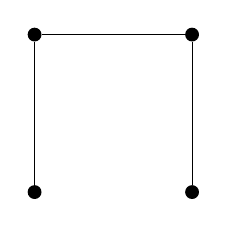
\begin{tikzpicture}[baseline={([yshift=-.5ex]current bounding box.center)}]
                \node[fill, circle, inner sep = 0, minimum size = 5pt] at (0, 0) (1) {};
                \node[fill, circle, inner sep = 0, minimum size = 5pt] at (2, 0) (2) {};
                \node[fill, circle, inner sep = 0, minimum size = 5pt] at (0, -2) (3) {};
                \node[fill, circle, inner sep = 0, minimum size = 5pt] at (2, -2) (4) {};
                \draw (1) -- (2);
                \draw (1) -- (3);
                \draw (2) -- (4);
            \end{tikzpicture}
        \end{gather*}
        Higher powers of a given coordinate would then, for example, give rise to diagrams with loops at a given vertex:
        \begin{gather*}
            A^{-1}_{11}A^{-1}_{12}A^{-1}_{22} =
            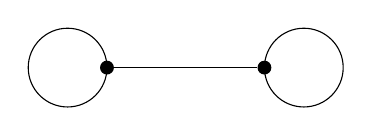
\begin{tikzpicture}[baseline={([yshift=-.5ex]current bounding box.center)}]
                \node[fill, circle, inner sep = 0, minimum size = 5pt] at (0, 0) (1) {};
                \node[fill, circle, inner sep = 0, minimum size = 5pt] at (2, 0) (2) {};
                \draw (-0.5, 0) circle (0.5);
                \draw (1) -- (2);
                \draw (2.5, 0) circle (0.5);
            \end{tikzpicture}
        \end{gather*}
    \end{example}

    \begin{remark}[Normalization]
        In practice, one often divides all Gaussian integrals by the quantity $I(A,0)$ to cancel the normalization factor. In the functional setting, this is even imperative since, as mentioned above, the normalization factor diverges for infinite-dimensional spaces.
    \end{remark}

\subsection{Generalizations}

    \newdef{Henstock--Kurzweil integral\footnotemark}{\index{integral!Henstock--Kurzweil}\index{integral!Perron}\index{integral!Denjoy}\index{integral!Luzin}\index{gauge|seealso{integral, Denjoy}}\index{integral!McShane}
    \footnotetext{Also called the \textbf{Perron}, \textbf{Lusin}, \textbf{(narrow) Denjoy} or \textbf{gauge} integral.}
        Consider the usual definition of the (proper) Riemann integral, where tagged partitions $P$ of $[a,b]$ are chosen and the integral is obtained as the limit of the Riemann sums
        \begin{gather}
            I = \sum_Pf(x_i)(t_i-t_{i-1})
        \end{gather}
        as the mesh size of the partitions goes to zero.

        Now, to obtain the generalized integral, consider a strictly positive function $\delta:[a,b]\mathbb{R}^{>0}$, the \textbf{gauge function}. Given such a gauge, a tagged partition $P$ is said to be \textbf{$\delta$-fine} if
        \begin{gather}
            [t_{i-1},t_i]\subset[x_i-\delta(x_i),x_i+\delta(x_i)]
        \end{gather}
        for subintervals in the partition.\footnote{If the condition $x_i\in[t_{i-1},t_i]$ in the definition of tagged partitions is dropped, the \textbf{McShane integral} is obtained. This can be shown to be equivalent to the \textit{Lebesgue integral} (see \labelref{chapter:measure}).}

        If the integral exists, it is given by the number $I\in\mathbb{R}$ such that for all $\varepsilon>0$ there exists a gauge $\delta:[a,b]\rightarrow\mathbb{R}^{>0}$ such that, if $P$ is $\delta$-fine, then
        \begin{gather}
            \left\vert I-\sum_Pf(x_i)(t_i-t_{i-1})\right\vert<\varepsilon\,.
        \end{gather}
    }
    \begin{remark}[Riemann integral]\index{integral!Riemann}
        If the gauge functions are chosen to be constant, the classical $(\varepsilon,\delta)$-definition of ordinary Riemann integrals is obtained.
    \end{remark}

    The following statement can be seen as a refinement of \cref{topology:heine_borel}. Moreover, it is also sometimes known as the \textbf{Borel--Lebesgue theorem}.\index{Borel--Lebesgue}
    \begin{property}[Cousin]\index{Cousin}
        For every gauge $\delta:[a,b]\rightarrow\mathbb{R}^{>0}$, there exists a $\delta$-fine partition. 
    \end{property}

    \begin{property}[Integrability]
        If $f:[a,b]\rightarrow\mathbb{R}$ is bounded, then the following are equivalent:
        \begin{itemize}
            \item $f$ is Henstock--Kurzweil integrable, and
            \item $f$ is \textit{Lebesgue integrable} (see \labelref{chapter:measure}).
        \end{itemize}
        More generally, a function $f:[a,b]\rightarrow\mathbb{R}$ is Henstock--Kurzweil integrable if and only if both $f$ and $|f|$ are \textit{Lebesgue integrable}.
    \end{property}

    The following property shows that `improper' Henstock--Kurzweil integrals are only truly improper for unbounded domains.
    \begin{property}[Hake]\index{Hake}
        \begin{gather}
            \Int_a^bf\,dx = \lim_{c\nearrow b}\Int_a^cf\,dx\,,
        \end{gather}
        whenever either side exists.
    \end{property}

    One of the most important arguments for using the Henstock--Kurzweil integral is its refinement of the Second Fundamental Theorem of Calculus~\ref{calculus:second_fundamental_theorem}. Note that the theorem for the Riemann integral required that the derivative was integrable. The gauge integral relaxes this condition.
    \begin{theorem}[Second fundamental theorem of calculus]
        Let $f:[a,b]\rightarrow\mathbb{R}$ be differentiable, then
        \begin{gather}
            \Int_a^xf'(x')\,dx' = f(x)-f(a)\text{\ \ a.e.}
        \end{gather}
    \end{theorem}

\section{Convexity}

    \newdef{Convex set}{\index{convex}\index{hull}\label{calculus:convex}
        A subset of $X$ of a vector space $V$ (\cref{linalgebra:vector_space}) is said to be convex if $x,y\in X$ implies that $\bigl\{\lambda x+(1-\lambda)y\mid\lambda\in[0,1]\bigr\}\subset X$, i.e.~if all straight lines connecting elements of the set are completely contained in that set. The \textbf{convex hull} of a subset $X$ is defined as the smallest convex subset containing $X$.
    }

    \newdef{Extreme point}{\index{extreme!point}\label{calculus:extreme_point}
        Consider a convex set $X$. The extreme points of $X$ are the points $p\in X$ such that, if
        \begin{gather}
            p = \lambda p_1 + (1-\lambda)p_2
        \end{gather}
        for some $p_1,p_2\in X$ and $\lambda\in[0,1]$, then $p_1=p_2=p$.
    }

    \newdef{Convex function}{\label{calculus:convex_function}
        Let $X$ be a convex set. A function $f:X\rightarrow\mathbb{R}$ is said to be convex if for all $x,y\in X$ and $\lambda\in[0,1]$:
        \begin{gather}
            f\bigl(\lambda x + (1-\lambda)y\bigr)\leq t\lambda(x) + (1-\lambda)f(y)\,.
        \end{gather}
        For the definition of a \textbf{concave} function, the inequality has to be turned around.
    }
    \newdef{Linear map}{\index{linear!map}
        A function $f:X\rightarrow\mathbb{R}$ is linear if and only if it is both convex and concave.
    }

    \begin{theorem}[Karamata's inequality]\index{Karamata}
        Consider an interval $I\subset\mathbb{R}$ and let $f:I\rightarrow\mathbb{R}$ be a convex function. If $(x_1,\ldots,x_n)$ is a tuple that majorizes $(y_1,\ldots,y_n)$, i.e.
        \begin{gather}
            \sum_{i=1}^nx_i = \sum_{i=1}^ny_i
        \end{gather}
        and
        \begin{gather}
            x_{(1)} + \cdots + x_{(k)}\geq y_{(1)} + \cdots + y_{(k)}
        \end{gather}
        for all $k\leq n$, where $x_{(i)}$ denotes the $i^{\text{th}}$ largest element of $(x_1,\ldots,x_n)$, then
        \begin{gather}
            \sum_{i=1}^nf(x_i)\geq\sum_{i=1}^nf(y_i)\,.
        \end{gather}
    \end{theorem}

    The following inequality can be derived directly from the definition of convexity by induction.
    \begin{theorem}[Jensen's inequality]\index{Jensen's inequality}\label{calculus:jensen_inequality}
        Let $f$ be a convex function and consider a point $\{a_i\}_{i\leq n}$ in the probability simplex $\Delta^n$ (\cref{topology:standard_simplex}).
        \begin{gather}
            f\left(\sum_{i=1}^na_ix_i\right)\leq\sum_{i=1}^na_if(x_i)\,.
        \end{gather}
    \end{theorem}

    \newdef{Legendre transformation}{\index{Legendre!transformation}\label{calculus:legendre}
        Consider a function $f:\mathbb{R}\rightarrow\mathbb{R}$. In certain cases (especially in physics) it is sometimes useful to replace the argument $x$ by the slope of $f$ at $x$, i.e.~to perform the transformation
        \begin{gather}
            x\longrightarrow f'(x)\,.
        \end{gather}
        However, it should be clear that this transformation is not always well-defined and, even if it is, it does not always preserve all the information contained in $f$.

        These conditions are satisfied exactly if $f$ is convex (or concave). In this case, the Legendre transform of $f$ is defined as
        \begin{gather}
            f^*(x^*) := \sup_x\bigl(x^*x - f(x)\bigr)\,.
        \end{gather}
        Now, consider the case where $f$ is differentiable. The above supremum can then be obtained by differentiating the right-hand side and equating it to zero. This results in $x^* = f'(x)$, which is exactly the transformation that was required. By expressing everything in terms of the Legendre tranformed quantity $x^*$, one can also find the derivative of $f^*$:
        \begin{gather}
            \deriv{f^*}{x^*}(x^*) = x(x^*)\,.
        \end{gather}
    }

    \begin{property}[Alternative characterization]\label{calculus:legendre_condition}
        In fact, up to an additive constant, the condition
        \begin{gather}
            (f^*)' = (f')^{-1}
        \end{gather}
        uniquely determines the Legendre transformation.
    \end{property}
    \begin{remark}
        These definitions can easily be extended to higher dimensions ($n\geq2$).
    \end{remark}

\section{Umbral calculus}\label{section:umbral_calculus}

    \newdef{Bernoulli polynomial}{\index{Bernoulli!polynomial}\label{calculus:bernoulli_number}
        The Bernoulli polynomials $B_n(x)$, for $n\in\mathbb{N}$, are generated as follows:
        \begin{gather}
            \frac{te^{xt}}{e^t-1} = \sum_{n=0}^{+\infty}B_n(x)\frac{t^n}{n!}\,.
        \end{gather}
        The Bernoulli numbers are defined as
        \begin{gather}
            B_n := B_n(0)\,.
        \end{gather}
    }

    \begin{property}[Recursion]\label{calculus:bernoulli_recursion}
        \begin{gather}
            B_n(x) = \sum_{k=0}^{+\infty}{n \choose k}B_kx^{n-k}
        \end{gather}
        or, more generally,
        \begin{gather}
            B_n(x+y) = \sum_{k=0}^{+\infty}{n \choose k}B_k(x)y^{n-k}
        \end{gather}
    \end{property}

    \begin{formula}[Differential formula]
        \begin{gather}
            B_n(x) = \frac{D}{e^D-1}x^n\,,
        \end{gather}
        where $D\equiv\ds\deriv{}{x}$.
    \end{formula}

    The recursion formula shows that Bernoulli polynomials are a concrete example of a more general class of polynomial sequences.
    \newdef{Appell sequence}{\index{Appell sequence}
        A sequence of polynomials $\seq{p}\subset\mathbb{R}[x]$ that satisfies
        \begin{gather}
            p_n(x+y) = \sum_{k=0}^n{n\choose k}p_k(x)y^{n-k}\,.
        \end{gather}
        This is equivalent to the following recursion relation
        \begin{gather}
            \deriv{p_n}{x} = np_{n-1}\,.
        \end{gather}
    }

    The second recursion relation for Appell sequences can be generalized to arbitrary linear operators. For so-called \textit{delta operators}\index{operator!delta}, i.e.~generalized derivative operators such as the \textit{forward differencing operator}, another important class of polynomials is recovered.
    \newdef{Sheffer sequence}{\index{Sheffer sequence}
        Let $Q:\mathbb{R}[x]\rightarrow\mathbb{R}[x]$ be a \textbf{delta operator}, i.e.~a shift-equivariant operator on polynomial functions that lowers the degree by 1:
        \begin{gather}
            Q\bigl(p(x+\lambda)\bigr) = Qp(x+\lambda)
        \end{gather}
        and
        \begin{gather}
            \deg(Qp) = \deg(p)-1
        \end{gather}
        for all $\lambda\in\mathbb{R}$ and $p\in\mathbb{R}[x]$.

        A polynomial sequence $\seq{p}\subset\mathbb{R}[x]$ is said to be a Sheffer sequence if
        \begin{gather}
            Qp_n = np_{n-1}\,.
        \end{gather}
    }
    \begin{example}
        Many common polynomials form Sheffer sequences, a few examples are Abel, Bernoulli, Euler, Hermite and Laguerre polynomials.
    \end{example}

    \begin{property}[Umbral composition]\index{umbral!composition}\label{calculus:umbral_composition}
        The Sheffer sequences form a group under the following composition law:
        \begin{gather}
            (p\circ q)_n(x) := \sum_{k=0}^na_{n,k}q_k(x) = \sum_{0\leq k\leq l\leq n}a_{n,k}b_{k,l}x^l
        \end{gather}
        where $p_n=\sum_{k=0}^nb_{n,k}x^k$ and $q_n=\sum_{k=0}^na_{n,k}x^k$. The identity element of the umbral group is given by the standard monomials $p_n(x)=x^n$.
    \end{property}

    \newdef{Binomial type}{\index{binomial!type}
        A polynomial sequence $\seq{p}\subset\mathbb{R}[x]$ is said to be of binomial type if
        \begin{gather}
            p_n(x+y) = \sum_{k=0}^n{n\choose k}p_k(x)p_{n-k}(y)\,.
        \end{gather}
        A Sheffer sequence is of binomial type if and only if
        \begin{itemize}
            \item $p_0(x)=1$, and
            \item $p_n(0)=0$ for all $n\in\mathbb{N}_0$.
        \end{itemize}
    }

    \begin{property}[Semidirect product]
        The umbral group is a semidirect product (\cref{group:inner_semidirect_product}) of the (Abelian) subgroup of Appell sequences and the subgroup of binomial type.

        This gives rise to a general recursion relation. Let $\seq{s}$ be a Sheffer sequence and consider the unique sequence $\seq{p}$ of binomial-type polynomials in the same coset as $s$.
        \begin{gather}
            s_n(x+y) = \sum_{k=0}^np_k(x)s_{n-k}(y)
        \end{gather}
    \end{property}

    Now, what about the term `umbral calculus'? In the $19^{\text{th}}$ century, some mathematicians noticed the apparent similarity between the binomial theorem~\ref{calculus:binomial_theorem} for monomials and the recursion relation~\ref{calculus:bernoulli_recursion} for Bernoulli polynomials. (This is, of course, explained by the fact that they are both Appell sequences.) This relation was, in turn, used to `prove' various statements about these polynomials. Passage from one sequence to another happens through a linear operator on the space of Appell sequences, as shown by \indexauthor{Rota}:
    \begin{gather}
        L_B:\mathbb{R}[x]\rightarrow\mathbb{R}[x]:x^n\mapsto B_n\,.
    \end{gather}
    The umbral composition rule is then simply given by the composition~\ref{calculus:umbral_composition} of two such linear operators.

\chapter{Complex calculus}

\section{Complex algebra}
	
	The set of complex numbers $\mathbb{C}$ forms a 2-dimensional vector space over the field of real numbers. Furthermore the operations of complex addition and complex multiplication also turn the complex numbers into a field.

	\newdef{Complex conjugate}{\index{complex conjugate}
    		The complex conjugate $\overline{z}:a+bi\mapsto a-bi$ is an involution, i.e. $\overset{=}{z} = z$. It is sometimes denoted by $z^*$ instead of $\overline{z}$.
	}
    
	\newformula{Real/imaginary part}{
		\nomenclature[O]{$\text{\text{Re}}$}{Real part of a complex number.}
		\nomenclature[O]{$\text{\text{Im}}$}{Imaginary part of a complex number.}
    		A complex number $z$ can also be written as $\text{Re}(z) + i\text{Im}(z)$ where
        	\begin{equation}
			\text{Re}(z) = \stylefrac{z + \overline{z}}{2}
		\end{equation}
        	\begin{equation}
			\text{Im}(z) = \stylefrac{z - \overline{z}}{2i}
		\end{equation}
	}
	\newdef{Argument}{\index{argument}
		\nomenclature[O]{$\text{arg}$}{Argument of a complex number.}
		Let $z$ be a complex number parametrized as $z = re^{i\theta}$. The number $\theta$ is called the argument of $z$ and it is denoted by $\arg(z)$.
	}
	
	\newdef{Riemann sphere}{\index{Riemann!sphere}
		Consider the one-point compactification\footnote{See definition \ref{topology:alexandrov_compactification}.} $\overline{\mathbb{C}} = \mathbb{C}\cup\{\infty\}$. This set is called the Riemann sphere or extended complex plane. The standard operations on $\mathbb{C}$ can be generalized to $\overline{\mathbb{C}}$ in the following way:
		\begin{align}
			z + \infty &= \infty\nonumber\\
			z * \infty &= \infty\\
			\frac{z}{\infty} &= 0\nonumber
		\end{align}
		for all non-zero $z \neq \infty$. As there exists no multiplicative inverse for $\infty$ the Riemann sphere does not form a field.
	}

\section{Holomorphic functions}
        
        \begin{definition}[Holomorphic]\index{holomorphic}
	        A function $f$ is holomorphic on an open set $U$ if it is complex differentiable at every point $z_0\in U$. 
        \end{definition}
        \newdef{Biholomorphic}{
        	A complex function $f$ is said to be biholomorphic if both $f$ and $f^{-1}$ are holomorphic.
        }
        
        \begin{property}[Cauchy-Riemann conditions]\index{Cauchy!Cauchy-Riemann conditions}
	        A holomorphic function $f(z)$ satisfies the following conditions:
	        \begin{equation}
	                \label{complexcalculus:cauchy_riemann}
	                \boxed{\pderiv{u}{x} = \pderiv{v}{y} \text{\qquad and\qquad} \pderiv{u}{y} = -\pderiv{v}{x}}
	        \end{equation}
	        or equivalently:
	        \begin{equation}
	                \label{complexcalculus:holomorphic_alternative_condition}
	                \boxed{\pderiv{f}{\overline{z}} = 0}
	        \end{equation}
        \end{property}
        
        \begin{theorem}[Looman-Menchoff\footnotemark]
        	\footnotetext{This is the strongest (most general) theorem on the holomorphy of continuous functions as it generalizes the original results by Riemann and Cauchy-Goursat.}
        	Let $f(z)$ be a continuous complex-valued function defined on a subset $U\in\mathbb{C}$. If the partial derivatives of the real and imaginary part exist and if $f$ satisfies the Cauchy-Riemann conditions then $f$ is holomorphic on $U$.
        \end{theorem}

	\begin{property}
		Functions $u,v$ satisfying the CR-conditions are harmonic functions, i.e. they satisfy Laplace's equation.
	\end{property}
	\begin{property}
		Functions $u,v$ satisfying the CR-conditions have orthogonal level curves \ref{set:level_set}.
	\end{property}

\section{Complex integrals}
		
	In this and further sections, all contours have been chosen to be evaluated counterclockwise (by convention). To obtain results concerning clockwise evaluation, most of the time adding a minus sign is sufficient.
        
        \newdef{Contour}{\index{contour}
        	A contour is a curve $z(t)$ that can be parametrized by
	        \begin{equation}
			\left.
			\begin{array}{c}
                	x = x(t)\\
        	        y = y(t)
        	        \end{array}\right\}
        	        \rightarrow z(t) = z = x+iy
		\end{equation}
        }
        \newformula{Complex contour integral}{
        	The complex contour integral of a function $f(z) = u(z) + iv(z)$ is defined as the following line integral:
        	\begin{equation}
        	    	\label{complexcalculus:contour_integral}
			\int_{z_1}^{z_2}f(z)dz = \int_{(x_1,y_1)}^{(x_2,y_2)}[u(x,y) + iv(x,y)](dx + idy)
		\end{equation}
        }
        
        \begin{theorem}[Cauchy's Integral Theorem\footnotemark]\index{Cauchy!integral theorem}
        	\footnotetext{Also called the \textit{Cauchy-Goursat theorem}.}
        	Let $\Omega$ be a simply-connected subset of $\mathbb{C}$ and let $f$ be a holomorphic function on $\Omega$. Then for every closed rectifiable contour $C$  in $\Omega$:
        	\begin{equation}
			\label{complexcalculus:cauchy_integral_theorem}
        	        \boxed{\oint_C f(z) dz = 0}
		\end{equation}
        \end{theorem}
        \result{The contour integral of a holomorphic function depends only on the limits of integration and not on the contour connecting them.}
        
        \begin{formula}[Cauchy's Integral Formula]\index{Cauchy!integral formula}
        	Let $\Omega$ be a connected subset of $\mathbb{C}$ and let $f$ be a holomorphic function on $\Omega$. Let $C$ be a contour in $\Omega$. For every point $z_0$ inside $C$ we find:
        	\begin{equation}
			\label{complexcalculus:cauchy_integral_formula}
        	        \boxed{f(z_0) = \frac{1}{2\pi i}\oint_C \frac{f(z)}{z - z_0} dz}
		\end{equation}
        \end{formula}

        \begin{result}[Analytic function]\index{analytic}
		Let $\Omega$ be a connected subset of $\mathbb{C}$ and $C$ a closed contour in $\Omega$. If $f$ is holomorphic on $\Omega$ then $f$ is analytic\footnotemark\ on $\Omega$ and:
	        \begin{equation}
			\label{complexcalculus:cauchy_integral_formula_derivative}
	                \boxed{f^{(n)}(z_0) = \frac{1}{2\pi i}\oint_C f(z) \frac{n!}{(z - z_0)^{n+1}} dz}
		\end{equation}
	        Furthermore, the derivatives are also holomorphic on $\Omega$.
	        \footnotetext{See definition \ref{calculus:analytic}.}
	\end{result}
        
        \begin{theorem}[Morera's Theorem]\index{Morera's theorem}
	        If $f$ is continuous on a connected open set $\Omega$ and $\oint_C f(z) dz = 0$ for every closed contour $C$ in $\Omega$, then $f$ is holomorphic on $\Omega$.
	\end{theorem}
        
        \begin{definition}[Meromorphic]\index{meromorphic}
		A function $f$ is called meromorphic when it is analytic on the whole complex plane with exception of isolated poles and removable singularities.
	\end{definition}

	\begin{theorem}[Sokhotski-Plemelj]\index{Sokhotski-Plemelj theorem}
		Let $f(x)$ be a continuous complex-valued function defined on the real line and let $a<0<b$.
		\begin{equation}
			\lim_{\varepsilon\rightarrow0^+}\int_a^b\frac{f(x)}{x\pm i\varepsilon}dx = \mp i\pi f(0) + \mathcal{P}\int_a^b\frac{f(x)}{x}dx
		\end{equation}
		where $\mathcal{P}$ denotes the Cauchy principal value.
	\end{theorem}
        
\section{Laurent series}
    	
    	\begin{definition}[Laurent series]\index{Laurent!series}\label{complexcalculus:laurent_series}
        	If $f$ is function, analytic on an annulus A, then $f$ can be expanded as the following series:
        	\begin{equation}
        	        f(z) = \sum^{\infty}_{n=-\infty} a_n (z - z_0)^n \qquad \text{with} \qquad a_n = \frac{1}{2\pi i} \oint \frac{f(z')}{(z' - z_0)^{n+1}} dz'
		\end{equation}
	\end{definition}
        
        \begin{remark}
		The Laurent series of an analytic function $f$ converges uniformly to $f$ in the ring shaped region ('\textit{annulus}') $R_1 < |z - z_0| < R_2$, with $R_1$ and $R_2$ the distances from $z_0$ to the two closest poles.
        \end{remark}
        
        \newdef{Principal part}{\index{principal!part}
        	The principal part of a Laurent series is defined as the sum:
		\begin{equation}
	            	\sum_{n=-\infty}^{-1}a_n(z-z_0)^n
		\end{equation}
        }
    
\section{Singularities}
\subsection{Poles}
	
	\newdef{Pole}{\index{pole}
    		A function $f(z)$ has a pole of order $m>0$ at a point $z_0$ if its Laurent series at $z_0$ satisfies $\forall n<-m:a_n = 0$ and $a_{-m}\neq0$.
	}
    
	\newdef{Essential singularity}{\index{essential singularity}
    		A function $f(z)$ has an essential singularity at a point $z_0$ if its Laurent series at $z_0$ satisfies $\forall n\in\mathbb{N}:a_{-n}\neq0$, i.e. its Laurent series has infinitely many negative degree terms.
	}
    
	\begin{theorem}[Picard's great theorem]\index{Picard!great theorem}
		Let $f(z)$ be an analytic function with an essential singularity at $z_0$. On every punctured neighbourhood of $z_0$, $f(z)$ takes on all possible complex values, with at most a single exception, infinitely many times.
	\end{theorem}
    
	\newmethod{Frobenius transformation}{\index{Frobenius!transformation}
	  	To study the behaviour of a function $f(z)$ at $z\rightarrow\infty$, one should apply the Frobenius transformation $h = 1/z$ and study the limit $\lim_{h\rightarrow0}f(h)$.
	}

\subsection{Branch cuts}
	
	\newformula{Roots}{
    		Let $z\in\mathbb{C}$. The $n^{th}$ roots\footnotemark\ of $z = re^{i\theta}$ are given by:
        	\begin{equation}
			z^{1/n} = \sqrt[n]{r}\exp\left(i\frac{\theta + 2\pi k}{n}\right)
		\end{equation}
        	where $k\in\{0,1,...,n\}$.
		\footnotetext{Also see the \textit{fundamental theorem of algebra} \ref{linalgebra:fundamental_theorem_of_algebra}.}
	}
	\newformula{Complex logarithm}{\index{logarithm}
		We parametrize $z$ as $z = re^{i\theta}$.
    		\begin{equation}
			\text{LN}(z) = \ln(r) + i(\theta + 2\pi k)
		\end{equation}
	}
	
	\newdef{Branch}{
		From these two formulas it is clear that the complex roots and logarithms are multi-valued functions. To get an unambiguous image it is necessary to fix a value of the parameter $k$. By doing so there will arise curves in the complex plane where the function is discontinuous. These are the branch cuts. A \textbf{branch} is then defined as a particular choice of the parameter $k$. For the logarithm the choice for $\arg(\text{LN})\in\ ]\alpha, \alpha + 2\pi]$ is often denoted by $\text{LN}_\alpha$ or $\log_\alpha$.	
	}
	\newdef{Branch point}{
    		Let $f(z)$ be a complex valued function. A point $z_0$ such that there exists no neighbourhood $|z-z_0|<\varepsilon$ where $f(z)$ is single valued is called a branch point.
	}
	\newdef{Branch cut}{
    		A line connecting exactly two branch points is called a branch cut. One of the branch points can be at infinity. In case of multiple branch cuts, they do not cross. 
	}
	
	
	\begin{example}
		Consider the complex function \[f(z) = \stylefrac{1}{\sqrt{(z-z_1)...(z-z_n)}}\] This function has singularities at $z_1,...,z_n$. If $n$ is even, this function will have $n$ (finite) branch points. This implies that the points can be grouped in pairs connected by non-intersecting branch cuts. If $n$ is odd, this function will have $n$ (finite) branch points and one branch point at infinity. The finite branch points will be grouped in pairs connected by non-intersecting branch cuts and the remaining branch point will be joined to infinity by a branch cut which does not intersect the others.(See \cite{branchcut} for the proof.)
	\end{example}

	\newdef{Principal value}{\index{principal!value}
		The principal value of a multi-valued complex function is defined as the choice of branch such that $\arg(f)\in]-\pi,\pi]$.
	}
    
\subsection{Residue theorem}
	
	\newdef{Residue}{
		\nomenclature[O]{$\text{Res}$}{Residue of a complex function.}
    		By applying formula \ref{complexcalculus:contour_integral} to a polynomial function we find:
    		\begin{equation}
    			\int_C(z-z_0)^ndz = 2\pi i\delta_{n,-1}
    		\end{equation}
    		where $C$ is a circular contour around the pole $z = z_0$. This means that integrating a Laurent series around a pole isolates the coefficient $a_{-1}$. This coefficient is therefore called the residue of the function at the given pole.
	}
	\begin{notation}
		The residue of a complex function $f(z)$ at a pole $z_0$ is denoted by $\text{Res}[f(z)]_{z=z_0}$.
	\end{notation}
	
	\begin{formula}
    		For a pole of order $m$, the residue is calculated as follows:
		\begin{equation}
			\label{complexcalculus:residue}
            		\operatorname{Res}\left[f(z)\right]_{z=z_j} = a_{-1} = \lim_{z\rightarrow z_0} \stylefrac{1}{(m - 1)!} \left(\pderiv{}{z}\right)^{m-1}\left(f(z)(z-z_0)\right)
		\end{equation}
	        For essential singularities the residue can be found by writing out the Laurent series explicitly.
	\end{formula}

	\begin{theorem}[Residue theorem]\index{Residue theorem}\label{complexcalculus:residue_theorem}
		If $f(z)$ is a meromorphic function in $\Omega$ and if $C$ is a closed contour in $\Omega$ which contains the poles $z_j$ of $f(z)$, then:
		\begin{equation}
                	\boxed{\oint_Cf(z)dz = 2\pi i\sum_j \operatorname{Res}\left[f(z)\right]_{z=z_j}}
		\end{equation}
	\end{theorem}
	\remark{For poles on the contour $C$, only half of the residue contributes to the integral.}
    
	\begin{formula}[Argument principle]\index{argument principle}
		Let $f(z)$ be a meromorphic function. Let $Z_f, P_f$ be respectively the number of zeroes and poles of $f(z)$ inside the contour $C$. From the residue theorem we can derive the following formula:
		\begin{equation}
			\frac{1}{2\pi i}\oint_C\frac{f(z)}{f'(z)}dz = Z_f - P_f
		\end{equation}
	\end{formula}
	\begin{formula}[Winding number]\index{winding number}\index{index}
		Let $f(z)$ be a meromorphic function and let $C$ be a simple closed contour. For all $a\not\in f(C)$ the winding number or \textbf{index} of $a$ with respect to the function $f$ is defined as:
		\begin{equation}
			\text{Ind}_f(a) = \frac{1}{2\pi i}\oint_C\frac{f'(z)}{f(z) - a}dz
		\end{equation}
		This number will always be an integer.
	\end{formula}

\section{Limit theorems}

    	\begin{theorem}[Small limit theorem]\index{Limit theorem}\label{complexcalculus:theorem:small_limit}
		Let $f$ be a function that is holomorphic almost every where on $\mathbb{C}$. Let the contour $C$ be a circular segment with radius $\varepsilon$ and central angle $\alpha$.
		If $z$ is parametrized as $z = \varepsilon e^{i\theta}$ then\[\int_Cf(z)dz = i\alpha A\] with \[A = \lim_{\varepsilon\rightarrow0}f(z)\]
	\end{theorem}
	
        \begin{theorem}[Great limit theorem]\label{complexcalculus:theorem:great_limit}
		Let $f$ be a function that is holomorphic almost every where on $\mathbb{C}$. Let the contour $C$ be a circular segment with radius $R$ and central angle $\alpha$. If $z$ is parametrized as $z = Re^{i\theta}$ then\[\int_Cf(z)dz = i\alpha B\] with \[B = \lim_{R\rightarrow+\infty}f(z)\]
	\end{theorem}
	
        \begin{theorem}[Jordan's lemma]\index{Jordan}\label{complexcalculus:theorem:jordan}
		Let $g$ be a continuous function with $g(z) = f(z)e^{bz}$. Let the contour $C$ be a semicircle lying in the half-plane bounded by the real axis and oriented away of the point $\overline{b}i$. If $z$ is parametrized as $z=Re^{i\theta}$ and \[\lim_{R\rightarrow\infty}f(z) = 0\] then\[\int_Cg(z)dz = 0\]
	\end{theorem}
		
\section{Analytic continuation}

	\begin{theorem}[Schwarz' reflection principle]\index{Schwarz!reflection principle}
		Let $f(z)$ be analytic on the upper half plane. If $f(z)$ is real when $z$ is real then
	        \begin{equation}
	        	f(\overline{z}) = \overline{f(z)}
	        \end{equation}
	\end{theorem}

\chapter{Measure theory and Lebesgue integration}
\label{chapter:lebesgue}

\section{Measure}
\subsection{General definitions}

	\newdef{Measure}{\index{measure}\index{$\sigma$-additivity}
    	\label{lebesgue:measure}
		Let $X$ be a set. Let $\Sigma$ be a $\sigma$-algebra over $X$. A function $\mu:\Sigma\rightarrow\overline{\mathbb{R}}$ is called a measure if it satisfies the following conditions:
		\begin{enumerate}
			\item Non-negativity: $\forall E\in\Sigma:\mu(E) \geq0$
            \item Null empty set: $\mu(\emptyset) = 0$
            \item Countable-additivity\footnotemark\ : $\forall i\neq j:E_i\cap E_j=\emptyset\implies\mu\left(\bigcup_{i=1}^\infty E_i\right) = \sum_{i=1}^\infty \mu(E_i)$
		\end{enumerate} 
    }
    \footnotetext{also called $\sigma$-additivity}
    
    \newdef{Measure space}{
    	\label{lebesgue:measure_space}
    	The pair $(X, \Sigma)$ is called a measurable space. The elements $E\in\Sigma$ are called measurable sets. The triplet $(X, \Sigma, \mu)$ is called a measure space.
    }
    
	\newdef{Almost everywhere\footnotemark}{
		\footnotetext{In probability theory this is foten often called \textbf{almost surely}.}
		Let $(X, \Sigma, \mu)$ be a measure space. A property $P$ is said to hold on X almost everywhere (a.e.) if it satisfies the following equation:
	        \begin{equation}
		        \label{lebesgue:almost_everywhere}
        		\mu\left(\{x\in X:\neg P(x)\}\right) = 0
        	\end{equation}
	}
    
    \newdef{Complete measure space}{
    	The measure space $(X,\Sigma,\mu)$ is said to be complete if for every $E\in\Sigma$ with $\mu(E) = 0$ the following property holds for all $A\subset E$:
        \[
        	A\in\Sigma \quad\text{and}\quad \mu(A) = 0
		\]
    }
    \newdef{Completion}{
    	Let $\mathcal{F},\mathcal{G}$ be $\sigma$-algebras over a set $X$. $\mathcal{G}$ is said to be the completion of $\mathcal{F}$ if it is the smallest $\sigma$-algebra such that the measure space $(X,\mathcal{G},\mu)$ is complete.
    }
    
    \newdef{Regular Borel measure}{
    	Let $\mu$ be a non-negative countably additive set function defined on $\mathcal{B}$. $\mu$ is called a regular Borel measure if it satisifes following equations for every Borel set $B$:
    	\begin{equation}
			\label{lebesgue:regular_borel_measure}
            \begin{array}{ccl}
				\mu(B)& =& \inf\{\mu(O):O \text{ open}, O\supset B\}\\
                \mu(B)& =& \sup\{\mu(F):F \text{ closed}, F\subset B\}
			\end{array}
		\end{equation}
    }

	\newdef{\texorpdfstring{$\sigma$-}\ finite measure}{\index{$\sigma$-finite}
    	\label{lebesgue:sigma_finite_measure}
    	Let $(\Omega,\mathcal{F},P)$ be a measure space. The measure $P$ is said to be $\sigma$-finite if there exists a sequence $(A_i)_{i\in\mathbb{N}}$ of measurable sets such that $\bigcup_{i=1}^{+\infty}A_i = \Omega$ with $\forall A_i:P(A_i) < +\infty$.
    }
    
    \begin{method}
    	To show that two measures coincide on a $\sigma$-algebra, it suffices to show that they coincide on the generating sets and apply the monotone class theorem \ref{set:theorem:monotone_class}.
    \end{method}


	\subsection{Lebesgue measure}
    	\newformula{Length of an interval}{\index{length}
        	The length of an open interval $I=(a,b)$ is defined as:
            \begin{equation}
				\label{lebesgue:interval_length}
                l\left(I\right) = b-a
			\end{equation}
        }
        
        \newdef{Null set}{\index{null set}
        	A set $A\subset\mathbb{R}$ is called a null set if it can be covered by a sequence of intervals of arbitrarily small length: $\forall\varepsilon>0$ there exists a sequence $(I_n)_{n\in\mathbb{N}}$ such that
            \begin{equation}
				A \subseteq \bigcup_{n=1}^{+\infty}I_n
			\end{equation}
            with
            \begin{equation}
				\sum_{i=1}^{+\infty}l(I_n) < \varepsilon
			\end{equation}
        }
        \begin{theorem}
			Let $(E_i)_{i\in\mathbb{N}}$ be a sequence of null sets. The union $\bigcup_{i=1}^{+\infty}E_i$ is also null.
		\end{theorem}
        \result{
        	\label{lebesgue:theorem:countable_set_is_null}
            Any countable set is null.
		}
    
    	\newdef{Outer measure}{\index{outer measure}
        	Let $X\subseteq\mathbb{R}$ be an open set. The (Lebesgue) outer measure is defined as:
            \begin{equation}
				\label{lebesgue:outer_measure}
                \boxed{m^*(X) = \inf\left\{\sum_{i=1}^{+\infty} l(I_i)\text{ with }(I_i)_{i\in\mathbb{N}} \text{ a sequence of open intervals that covers }X\right\}}
			\end{equation}
        }
        
        \begin{property}
			Let $I$ be an interval. The outer measure equals the length: $m^*(I) = l(I)$.
		\end{property}
        \begin{property}
			The outer measure is translation invariant: $m^*(A + t) = m^*(A)\quad,\forall A,t$
		\end{property}
        \begin{property}
			$m^*(A) = 0$ if and only if $A$ is null.
		\end{property}
        \begin{property}
			If $A\subset B$ then $m^*(A)\leq m^*(B)$.
		\end{property}
        \begin{property}[Countable subadditivity]
        	For every sequence of sets $(E_i)_{i\in\mathbb{N}}$ the following inequality holds: 
			\begin{equation}
				m^*\left(\bigcup_{i=1}^{+\infty}E_i\right) \leq \sum_{i=1}^{+\infty}m^*(E_i)
			\end{equation}
		\end{property}
        
        \begin{theorem}[Carath\'eodory's criterion / Lebesgue measure]
        	\index{Carath\'eodory!criterion}\index{Lebesgue!measure}\index{measurable!set}
        	Let $X$ be a set. If $X$ satisfies the following equation, it is said to be Lebesgue measurable:
            \begin{equation}
				\label{lebesgue:lebesgue_measure}
                \forall E\subseteq\mathbb{R}:m^*(E) = m^*(E\cap X) + m^*(E\cap X^c)
			\end{equation}
            This is denoted by $X\in\mathcal{M}$ and the outer measure $m^*(X)$ is called the Lebesgue measure of $X$ denoted by $m(X)$.
        \end{theorem}
        \begin{property}
			All null sets and intervals are measurable.
		\end{property}
        \newprop{Countable additivity}{\index{countable!additivity}
        	For every sequence $(E_i)_{i\in\mathbb{N}}$ with $E_i\in\mathcal{M}$ satisfying $i\neq j:E_i\cap E_j = \emptyset$ the following equation holds:
        	\begin{equation}
				\boxed{m\left(\bigcup_{i=1}^{+\infty}E_i\right) = \sum_{i=1}^{+\infty}m(E_i)}
			\end{equation}
        }
        \sremark{Previous property, together with the properties of the outer measure, implies that the Lebesgue measure is indeed a proper measure as defined in \ref{lebesgue:measure}.}
        
        \begin{property}
			$\mathcal{M}$ is a $\sigma$-algebra\footnotemark\ over $\mathbb{R}$. 
		\end{property}
        \footnotetext{See definition \ref{set:sigma_algebra}.}
        
        \begin{theorem}
			For every $A\subset\mathbb{R}$ there exists a sequence $(O_i)_{i\in\mathbb{N}}$ of open sets such that:
            \begin{equation}
            	\label{lebesgue:theorem:open_cover_existence}
				A\subset\bigcap_iO_i\qquad\text{and}\qquad m\left(\bigcap_iO_i\right) = m^*(A)
			\end{equation}
		\end{theorem}
        \begin{theorem}
			For every $E\in\mathcal{M}$ there exists a sequence $(F_i)_{i\in\mathbb{N}}$ of closed sets such that:
            \begin{equation}
            	\label{lebesgue:theorem:closed_cover_existence}
				\bigcup_iF_i\subset E\qquad\text{and}\qquad m\left(\bigcup_iF_i\right) = m(E)
			\end{equation}
		\end{theorem}
        \sremark{The previous 2 theorems imply that the Lebesgue measure is a regular Borel measure \ref{lebesgue:regular_borel_measure}.}
        
        \begin{theorem}
			Let $E\subset\mathbb{R}$. $E\in\mathcal{M}$ if and only if for every $\varepsilon>0$ there exist an open set $O\supset E$ and a closed set $F\subset E$ such that $m^*(O\backslash E) < \varepsilon$ and $m^*(E\backslash F)<\varepsilon$.
		\end{theorem}
        
        \begin{property}
			Let $(A_i)_{i\in\mathbb{N}}$ be a sequence of sets with $\forall i:A_i\in\mathcal{M}$. The following two properties apply:
            \begin{equation}
            	\forall i: A_i\subseteq A_{i+1} \implies m\left(\bigcup_{i=1}^{+\infty}A_i\right) = \lim_{i\rightarrow+\infty}m(A_i)
			\end{equation}
            \begin{equation}
            	\forall i: A_i\supseteq A_{i+1} \land m(A_1)<+\infty\implies m\left(\bigcap_{i=1}^{+\infty}A_i\right) = \lim_{i\rightarrow+\infty}m(A_i)
			\end{equation}
		\end{property}
        \remark{This property is not only valid for the Lebesgue measure but for every countably additive set function.}
        \begin{property}
			The Lebesgue measure $m(X)$ is continuous at $\emptyset$, i.e. if $(A_i)_{i\in\mathbb{N}}\rightarrow\emptyset$ then $\displaystyle\lim_{i\rightarrow+\infty}m(A_i) = 0$.
		\end{property}
        
        \begin{theorem}
			$\mathcal{M}$ is the completion of $\mathcal{B}$.
		\end{theorem}
        \result{
        	\label{lebesgue:theorem:B_in_M}
        	$\mathcal{B}\subset\mathcal{M}\subset\mathcal{F}_{\mathbb{R}}$
		}
        
        \newdef{Restricted Lebesgue measure}{\index{Lebesgue!restricted measure}
        	Let $B\subset\mathbb{R}$ be a measurable set with measure $m(B)>0$. The restriction of the Lebesgue measure to the set $B$ is defined as follows:
            \begin{equation}
				\label{lebesgue:restricted_lebesgue_measure}
                \mathcal{M}_B = \left\{A\cap B:A\in\mathcal{M}\right\}\qquad\text{and}\qquad\forall E\in\mathcal{M}_B:m_B(E) = m(E)
			\end{equation}
            Furthermore, the measure space $(B,\mathcal{M}_B,m_B)$ is complete.
        }
        
    \subsection{Measurable functions}
    	\newdef{Measurable function}{\index{measurable!function}
        	\label{lebesgue:measurable_function}
        	A function $f$ is (Lebesgue) measurable if for every interval $I\subset\mathbb{R}:f^{-1}(I)\in\mathcal{M}$.
        }
        \newdef{Borel measurable function}{\index{Borel!measurable function}
        	\label{lebesgue:borel_measurable_function}
        	A function $f$ is called Borel measurable\footnotemark\ if for every interval $I\subset\mathbb{R}:f^{-1}(I)\in\mathcal{B}$.
        }
        \footnotetext{These functions are often simply called 'Borel functions'.}
        \remark{Inclusion \ref{lebesgue:theorem:B_in_M} implies that every Borel function is also Lebesgue measurable.}
        
        \begin{theorem}
			The class of Lebesgue measurable\footnotemark\ functions defined on $E\in\mathcal{M}$ is closed under multiplication and it forms a vector space.
		\end{theorem}
        \footnotetext{This property is also valid for Borel functions.}
        
        \begin{property}
			Following types of functions are measurable:
            \begin{itemize}
				\item monotone functions
                \item continuous functions
                \item indicator functions
			\end{itemize}
		\end{property}
		\begin{result}
			Let $f,g$ be measurable functions. Let $F:\mathbb{R}\times\mathbb{R}\rightarrow\mathbb{R}$ be a continuous function. The composition $F(f(x), g(x))$ is also measurable.
		\end{result}
        
        \begin{property}
			Let $f$ be a measurable function. The set\footnotemark\ $\{x:f(x) = a\}$ is also measurable for all $a\in\mathbb{R}$.
		\end{property}
        \footnotetext{This set is called the 'level set' of $f$.}

        \begin{theorem}
			Define following functions, which are measurable if $f$ is measurable as a result of previous properties:
            \begin{equation}
				\label{lebesgue:positive_part}
                f^+(x) = \left\{
                \begin{array}{ccc}
					f(x)&\text{if}&f(x)>0\\
                    0&\text{if}&f(x)\leq0
				\end{array}\right. = \max(f,0)
			\end{equation}
            \begin{equation}
				\label{lebesgue:negative_part}
                f^-(x) = \left\{
                \begin{array}{ccc}
					0&\text{if}&f(x)>0\\
                    -f(x)&\text{if}&f(x)\leq0
				\end{array}\right. = \max(-f,0)
			\end{equation}
            The function $f:E\rightarrow\mathbb{R}$ is measurable if and only if both $f^+$ and $f^-$ are measurable. Furthermore $f$ is measurable if $|f|$ is measurable, the converse is false.
		\end{theorem}

	\subsection{Limit operations}
    	\begin{property}
			Let $(f_i)_{i\in\mathbb{N}}$ be a sequence of measurable\footnotemark\ functions. The following operations are measurable:
            \begin{itemize}
				\item $\ds\min_{i\leq k}f_i$ and $\ds\max_{i\leq k}f_i$
                \item $\ds\inf_{i\in\mathbb{N}}f_i$ and $\ds\sup_{i\in\mathbb{N}}f_i$
                \item $\ds\liminf_{i\rightarrow+\infty}f_i$ and $\ds\limsup_{i\rightarrow+\infty}f_i$
			\end{itemize}
		\end{property}
        \footnotetext{This property is also valid for Borel functions.}
        \sremark{The measurability of the limit inferior and limit superior follows from their definitions and from the measurability of the $\inf/\sup$ and $\min/\max$.}
        
        \begin{property}
			Let $f$ be a measurable function. Let $g$ be a function such that $f=g$ almost everywhere. The function $g$ is measurable.
		\end{property}
        \result{A result of the previous two properties is the following: if a sequence of measurable functions converges pointwise a.e. then the limit is also a measurable function.}
	
        \newdef{Essential supremum}{\index{essential!supremum}
        	\begin{equation}
            	\label{lebesgue:essential_supremum}
                \esssup f = \sup\{z:f\geq z\text{ a.e.}\}
			\end{equation}
        }
        \newdef{Essential infimum}{\index{essential!infimum}
        	\begin{equation}
            	\label{lebesgue:essential_infimum}
                \essinf f = \inf\{z:f\leq z\text{ a.e.}\}
			\end{equation}
        }
        \begin{property}
			Let $f$ be a measurable function. $f\leq\esssup f\text{ a.e.}$ and $f\geq\essinf f\text{ a.e.}$ We also have that: $\esssup f\leq\sup f$ and $\essinf f\geq\inf f$, furthermore this last pair of inequalities becomes a pair of equalities if $f$ is continuous.
		\end{property}
        \begin{property}
			Let $f,g$ be measurable functions. $\esssup(f+g)\leq\esssup f + \esssup g$. An analogous inequality holds for the essential infimum.
		\end{property}

\section{Lebesgue integral}
	\subsection{Simple functions}
    	\newdef{Indicator function}{\index{indicator function}
        	An important function when working with sets is the following one:
            \begin{equation}
            	\label{lebesgue:indicator_function}
				\boxed{\mathbbm{1}_A(x) = \left\{
                \begin{array}{ccc}
					1&\text{if}&x\in A\\
                    0&\text{if}&x\not\in A
				\end{array}\right.}
			\end{equation}
        }
		\newdef{Simple function}{\index{simple function}
    		Let $f$ be a function that takes on a finite number of non-negative values $\{a_i\}$ with for every $i\neq j: f^{-1}(a_i)\cap f^{-1}(a_j) = \emptyset$. $f$ is called a simple function if it can be expanded in the following way:
        	\begin{equation}
				\label{lebesgue:simple_function}
            	f(x) = \sum_{i=1}^n a_i\mathbbm{1}_{A_i}(x)
			\end{equation}
        	with $A_i = f^{-1}(a_i)\in\mathcal{M}$
    	}
        \begin{remark}[Step function]\index{step function}
        	\label{lebesgue:step_function}
        	If the sets $A_i$ are intervals, the simple function is often called a 'step function'.
		\end{remark}
        
        \newformula{Lebesgue integral of simple functions}{\index{Lebesgue}
        	Let $\varphi$ be a simple function as defined in equation \ref{lebesgue:simple_function}. Let $\mu:\mathcal{M}\rightarrow\mathbb{R}$ be a Lebesgue measure and let $E$ be a measurable set. The Lebesgue integral of $\varphi$ over a $E$ with respect to $\mu$ is given by:
            \begin{equation}
				\label{lebesgue:integral_simple_function}
                \int_E\varphi d\mu = \sum_{i=1}^na_i\mu(E\cap A_i)
			\end{equation}
        }
        \begin{example}
			Let $\mathbbm{1}_\mathbb{Q}$ be the indicator function of the set of rational numbers. This function is clearly a simple function. Previous formula makes it possible to integrate the rational indicator function over the real line, which is not possible in the sense of Riemann:
            \begin{equation}
				\int_\mathbb{R}\mathbbm{1}_\mathbb{Q}dm = 1\times m(\mathbb{Q}) + 0\times m(\mathbb{R}\backslash\mathbb{Q}) = 0
			\end{equation}
            where the measure of the rational numbers is 0 because it is a countable set (see corollary \ref{lebesgue:theorem:countable_set_is_null}.
		\end{example}
        
	\subsection{Measurable functions}
        \newformula{Lebesgue integral}{\index{Lebesgue}
        	Let $f$ be a non-negative measurable function. Let $A$ be measurable set. The Lebesgue integral of $f$ over $E$ is defined as:
            \begin{equation}
				\label{lebesgue:integral}
                \int_Efdm = \sup\left\{\int_E\varphi dm:\varphi \text{ a simple function such that } \varphi\leq f\right\}
			\end{equation}
        }
        \begin{property}
			The Lebesgue integral $\int_Efdm$ of a measurable function $f$ is always non-negative.
		\end{property}
        
        \begin{notation}
        	The following notation is frequently used (both in the sense of Riemann and Lebesgue):
			\begin{equation}
				\int fdm = \int_\mathbb{R}fdm
			\end{equation}
		\end{notation}
        \begin{formula}
			The following equality is easily proved as for every set $A\subseteq\mathbb{R}:A\cup A^c = \mathbb{R}$.
            \begin{equation}
            	\label{lebesgue:interchanging_domains_with_indicator_function}
				\int_Afdm = \int f\mathbbm{1}_Adm
			\end{equation}
		\end{formula}
        
        \begin{theorem}
			Let $f$ be a non-negative measurable function. Then $f=0$ a.e. if and only if $\int_\mathbb{R} fdm = 0$.
		\end{theorem}
        \begin{property}
			The Lebesgue integral over a null set is 0.
		\end{property}
        \begin{property}\index{Mean value theorem}
			Let $f,g$ me measurable functions. The Lebesgue integral has the following properties:
            \begin{itemize}
            	\item $f\leq g$ a.e. implies $\int fdm\leq\int gdm$.
                \item Let $A$ be a measurable set. Let $B\subset A$. Then $\int_B fdm\leq\int_A fdm$.
                \item The Lebesgue integral is linear.
                \item For every two disjoint measurable sets $A$ and $B$ we have that $\int_{A\cup B}fdm = \int_A fdm + \int_B fdm$.
                \item \textbf{Mean value theorem}: If $a\leq f(x)\leq b$, then $am(A)\leq\int_Afdm\leq bm(A)$.
			\end{itemize}
		\end{property}
        
        \begin{theorem}
			Let $f$ be a non-negative measurable function. There exists an increasing sequence $(\varphi_i)_{i\in\mathbb{N}}$ of simple functions such that $\varphi_i\nearrow f$.
		\end{theorem}
        \begin{theorem}
			Let $f$ be a bounded measurable function defined on the interval $[a,b]$. For every $\varepsilon>0$ there exists a step function\footnotemark\ $h$ such that $\int_a^b|f-h|dm<\varepsilon$.
		\end{theorem}
        \footnotetext{See remark \ref{lebesgue:step_function}.}
        

\subsection{Integrable functions}
        \newdef{Integrable function}{\index{integrable}
        	Let $E\in\mathcal{M}$. A measurable function $f$ is said to be integrable over $E$ if both $\int_Ef^+dm$ and $\int_Ef^-dm$ are finite. The Lebesgue integral of $f$ over $E$ is defined as:
            \begin{equation}
				\label{lebesgue:integrable_function}
                \int_E fdm = \int_E f^+dm - \int_E f^-dm
			\end{equation}
        }
        \sremark{The difference between the integral \ref{lebesgue:integral} and the integral of an integrable function is that with the latter $f$ does not have to be non-negative.}
        
        \begin{theorem}
			$f$ is integrable if and only if $|f|$ is integrable. Furthermore, $\int_E|f|dm = \int_E f^+dm + \int_E f^-dm$.
		\end{theorem}
        \begin{property}
			Let $f,g$ be integrable functions. The following important properties apply:
            \begin{itemize}
				\item $f+g$ is also integrable.
                \item $\forall E\in\mathcal{M}, \int_Efdm\leq\int_Egdm\implies f\leq g$ a.e.
                \item Let $c\in\mathbb{R}$. $\int_E(cf)dm = c\int_Efdm$.
                \item $f$ is finite a.e.
                \item $|\int fdm|\leq\int|f|dm$
                \item $f\geq0\land\int fdm=0\implies f=0$ a.e.
			\end{itemize}
		\end{property}
        
        \begin{theorem}\index{L$^1$}
        	\label{lebesgue:L1}
			The set of functions integrable over a set $E\in\mathcal{M}$ forms a vector space. It is denoted by $\mathcal{L}^1(E)$.
		\end{theorem}
        
        \begin{property}
        	Let $f\in\mathcal{L}^1$ and $\varepsilon>0$. There exists a continuous function $g$, vanishing outside some finite interval, such that $\int|f-g|dm<\varepsilon$.
		\end{property}
        
        \begin{property}\index{continuity!absolute continuity}
        	\label{lebesgue:theorem:measure_by_integral}
			Let $f\geq0$. The mapping $E\mapsto\int_Efdm$ is a measure on $E$ (if it exists, hence if $f$ is integrable). Furthermore, this measure is said to be \textbf{absolutely continuous}.
		\end{property}
        \sremark{See section \ref{lebesgue:section:Radon-Nikodym} for further information.}

    \subsection{Convergence theorems}
    	\begin{theorem}[Fatou's lemma]\index{Fatou's lemma}
			Let $(f_n)_{n\in\mathbb{N}}$ be a sequence of non-negative measurable functions.
            \begin{equation}
				\label{lebesgue:theorem:fatous_lemma}
                \int_E\left(\liminf_{n\rightarrow\infty}f_n\right)dm \leq \liminf_{n\rightarrow\infty}\int_Ef_ndm
			\end{equation}
		\end{theorem}
        \begin{theorem}[Monotone convergence theorem]\index{monotone}\index{monotone convergence theorem}
			Let $E\in\mathcal{M}$. Let $(f_n)_{n\in\mathbb{N}}$ be an increasing sequence of non-negative measurable functions such that $f_n\nearrow f$ pointwise a.e. We have the following powerful equality:
            \begin{equation}
				\label{lebesgue:theorem:monotone_convergence_theorem}
                \boxed{\int_E fdm = \lim_{n\rightarrow\infty}\int_E f_n(x)dm}
			\end{equation}
		\end{theorem}
        
        \begin{method}
        	 \label{lebesgue:method:linear_proofs}
			To prove 'linear' results concerning integrable functions in spaces such as $\mathcal{L}^1(E)$ we proceed according to the following steps:
            \begin{enumerate}
            	\item Verify that the property holds for indicator functions. (This often follows by definition.)
                \item Use the linearity to extend the property to simple functions.
                \item Apply the monotone convergence theorem to show that the property holds for all non-negative measurable functions.
                \item Extend the property to all integrable functions by writing $f = f^+ - f^-$ and applying the linearity again.
			\end{enumerate}
		\end{method}
        
        \begin{theorem}[Dominated convergence theorem]\index{dominated convergence theorem}
			Let $E\in\mathcal{M}$. Let $(f_n)_{n\in\mathbb{N}}$ be a sequence of measurable functions with $\forall n:|f_n|\leq g$ a.e. for a function $g\in\mathcal{L}^1(E)$. If $f_n\rightarrow f$ pointwise a.e. then $f$ is integrable over $E$ and
            \begin{equation}
				\label{lebesgue:theorem:dominated_convergence_theorem}
                \int_E fdm = \lim_{n\rightarrow\infty}\int_E f_n(x)dm
			\end{equation}
		\end{theorem}
        
        \begin{property}
			Let $(f_n)_{n\in\mathbb{N}}$ be a sequence of non-negative measurable functions. The following equality applies:
            \begin{equation}
				\int\sum_{n=1}^{+\infty}f_n(x)dm = \sum_{n=1}^{+\infty}\int f_n(x)dm
			\end{equation}
            We cannot conclude that the right-hand side is finite a.e., so the series on the left-hand side need not be integrable.
		\end{property}
        
        \begin{theorem}[Beppo-Levi]\index{Levi|see{Beppo-Levi}}\index{Beppo-Levi}
			Suppose that
            \[\sum_{i=1}^\infty\int|f_n|(x)dm\text{ is finite.}\]
            The series $\sum_{i=1}^\infty f_n(x)$ converges a.e. Furthermore, the series is integrable and
            \begin{equation}
				\label{lebesgue:theorem:beppo_levi}
                \int\sum_{i=1}^\infty f_n(x)dm = \sum_{i=1}^\infty\int f_n(x)dm
			\end{equation}
		\end{theorem}
        
        \begin{theorem}[Riemann-Lebesgue lemma]\index{Riemann!Riemann-Lebesgue lemma}\label{lebesgue:riemann_lebesue_lemma}
			Let $f\in\mathcal{L}^1$. The sequences \[s_k = \int_{-\infty}^{+\infty}f(x)\sin(kx)dx\] and \[c_k = \int_{-\infty}^{+\infty}f(x)\cos(kx)dx\] both converge to 0.
		\end{theorem}
        \sremark{This theorem is useful in Fourier analysis.}

\subsection{Relation to the Riemann integral}
	\begin{theorem}[Fundamental theorem of calculus]
		If $f:[a,b]\rightarrow\mathbb{R}$ is continuous then $f$ is integrable and the function $F:x\mapsto\int_a^xfdm$ is differentiable for $x\in]a,b[$ such that $F'=f$.
	\end{theorem}
    
    \begin{theorem}
		Let $f:[a,b]\rightarrow\mathbb{R}$ be a bounded function.
        \begin{itemize}
        	\item $f$ is Riemann-integrable if and only if $f$ is continuous a.e. with respect to the Lebesgue measure on $[a,b]$.
            \item Riemann-integrable functions on $[a,b]$ are integrable with respect to the Lebesgue measure on $[a,b]$ and the integrals coincide.
		\end{itemize}
	\end{theorem}
    
    \begin{theorem}
		If $f\geq0$ and the improper Riemann integral \ref{calculus:improper_integral} exists, then the Lebesgue integral $\int fdm$ exists and the two integrals coincide.
	\end{theorem}

\section{Examples}
    	\newdef{Dirac measure\footnotemark}{\index{Dirac}
        	\footnotetext{Compare to \ref{distribution:dirac_delta}. }
        	We define the Dirac measure as follows:
            \begin{equation}
				\label{lebesgue:dirac_measure}
                \delta_a(X) = \left\{\begin{array}{cc}
                	1&\text{if } a\in X\\
                    0&\text{if } a\not\in X\\
                \end{array}\right.
			\end{equation}
            The integration with respect to the Dirac measure has the following nice property\footnotemark:
            \begin{equation}
				\int g(x)d\delta_a = g(a)
			\end{equation}
        }
        \footnotetext{This equality can be proved by applying formula \ref{prop:change_of_variable} with $X\equiv a$.}
        \begin{example}
			Let $\mu=\delta_2, X = (-4;1)$ and $Y = (-2;17)$. The following two integrals are easily computed:
            \[\int_Xd\mu = 0\]
            \[\int_Yd\mu = 1\]
		\end{example}

\section{Space of integrable functions}
\subsection{Distance}\index{distance}
	To define a distance between functions, we first have to define some notion of length of a function. Normally this would not be a problem, because we now do know how to integrate integrable functions, however the fact that two functions differing on a null set have the same integral carries problems with it, i.e. a non-zero function could have a zero length. Therefore we will define the 'length' on a different vector space:\par
    
    \noindent Define the following set of equivalence classes $L^1(E) = \mathcal{L}^1(E)_{/\equiv}$ by introducing the equivalence relation: $f\equiv g$ if and only if $f=g$ a.e.
    \begin{property}
		$L^1(E)$ is a Banach space\footnotemark.
	\end{property}
    \footnotetext{See definition \ref{linalgebra:banach_space}.}
    
    \begin{formula}
		A norm on $L^1(E)$ is given by:
        \begin{equation}
			\label{lebesgue:L1_norm}
            ||f||_1 = \int_E |f|dm
		\end{equation}
	\end{formula}
    
\subsection{Hilbert space \texorpdfstring{$L^2$}\ }\index{Hilbert!space|see{L$^2$}}\index{L$^2$}
	\label{lebesgue:section:hilbert_space}
    
    \begin{property}
    	\label{lebesgue:L2_hilbert_space}
		$L^2$ is a Hilbert space\footnotemark.
	\end{property}
    \footnotetext{See definition \ref{hilbert:hilbert_space}.}
	\begin{formula}
		A norm on $L^2(E)$ is given by:
        \begin{equation}
			\label{lebesgue:L2_norm}
            ||f||_2 = \left(\int_E |f|^2dm\right)^{\frac{1}{2}}
		\end{equation}
        This norm is induced by the following inner product:
        \begin{equation}
			\label{lebesgue:L2_inner_product}
            \boxed{\langle f|g \rangle = \int_E f\overline{g}dm}
		\end{equation}
	\end{formula}
    Now instead of deriving $L^2$ from $\mathcal{L}^2$ we do the opposite. We define $\mathcal{L}^2$ as the set of measurable functions for which equation \ref{lebesgue:L2_norm} is finite.
    
    \newdef{Orthogonality}{\index{orthogonality}
    	As $L^2$ is a Hilbert space and thus has an inner product $\langle\cdot|\cdot\rangle$, it is possible to introduce the concept of orthogonality of functions in the following way:
        \begin{equation}
			\label{lebesgue:orthogonal_functions}
            \langle f|g \rangle = 0\implies\text{f and g are orthogonal}
		\end{equation}
        Furthermore it is also possible to introduce the angle between functions in the same way as equation \ref{linalgebra:angle}.
    }
    
    \begin{formula}[Cauchy-Schwarz inequality]\index{Cauchy!Cauchy-Schwarz inequality}
		Let $f,g\in L^2(E,\mathbb{C})$. We have that $fg\in L^1(E\mathbb{C})$ and:
        \begin{equation}
			\label{lebesgue:schwarz_inequality}
            \boxed{\left|\int_E f\overline{g}dm\right|\leq||fg||_1\leq||f||_2||g||_2}
		\end{equation}
	\end{formula}
    \sremark{This follows immediately from formula \ref{lebesgue:holders_inequality}.}
    
    \begin{property}
		If $E$ has finite Lebesgue measure then $L^2(E)\subset L^1(E)$.
	\end{property}
    
\subsection{\texorpdfstring{$L^p$}\ \ spaces}\index{L$^p$}
	Generalizing the previous two Lebesgue function classes leads us to the notion of $L^p$ spaces with the following norm:
    
    \begin{property}For all $1\leq p\leq+\infty$ $L^p(E)$ is a Banach space with a norm given by:
    	\begin{equation}
			\label{lebesgue:Lp_norm}
            ||f||_p = \left(\int_E |f|^p\ dm\right)^{\frac{1}{p}}
		\end{equation}
    \end{property}
    \remark{Note that $L^2$ is the only $L^p$ space that is also a Hilbert space. The other $L^p$ spaces do not have a norm induced by an inner product.}
    
    \newformula{H\"{o}lder's inequality}{\index{H\"older's inequality}
    	Let $\frac{1}{p} + \frac{1}{q} = 1$ with $p\geq1$. For every $f\in L^p(E)$ and $g\in L^q(E)$ we have that $fg\in L^1(E)$ and:
        \begin{equation}
        	\label{lebesgue:holders_inequality}
			||fg||_1\leq||f||_p||g||_q
		\end{equation}
    }
    \newformula{Minkowski's inequality}{\index{Minkowski!inequality}
    	For every $p\geq1$ and $f,g\in L^p(E)$ we have
        \begin{equation}
			\label{lebesgue:minkowskis_inequality}
            ||f+g||_p\leq||f||_p + ||g||_p
		\end{equation}
    }
    \begin{property}
		If $E$ has finite Lebesgue measure then $L^q(E)\subset L^p(E)$ when $1\leq p\leq q<+\infty$.
	\end{property}
    
\subsection{\texorpdfstring{$L^\infty$}\ \ space of essentially bounded measurable functions}
	\newdef{Essentially bounded function}{
    	Let $f$ be a measurable function satisfying $\esssup |f| <+\infty$. The function $f$ is said to be essentially bounded and the set of all such functions is denoted by $L^\infty(E)$.
    }
    
    \begin{formula}\index{supremum}
		A norm on $L^\infty$ is given by:
        \begin{equation}
			||f||_\infty = \esssup|f|
		\end{equation}	
        This norm is called the \textbf{supremum norm} and it induces the supremum metric \ref{topology:supremum_distance}.
	\end{formula}
    \begin{property}
		$L^\infty$ is a Banach space.
	\end{property}
	
\section{Product measures}
\subsection{Real hyperspace \texorpdfstring{$\mathbb{R}^n$}\ }
	
    The notions of intervals and lengths from the one dimensional case can be generalized to more dimensions in the following way:
    \newdef{Hypercube}{\index{hypercube}
    	Let $I_1, ..., I_n$ be a sequence of intervals.
    	\begin{equation}
			\mathbf{I} = I_1\times...\times I_n
		\end{equation}
    }
    \newdef{Generalized length}{
    	Let $\mathbf{I}$ be a hypercube induced by the sequence of intervals $I_1,...,I_n$. The length of $\mathbf{I}$ is given by:
        \begin{equation}
			l(\mathbf{I}) = \prod_{i=1}^{n}l(I_i)
		\end{equation}
    }
    
\subsection{Construction of the product measure}

    \newprop{General condition}{
    	The general condition for multi-dimensional\newline Lebesgue measures is given by following equation which should hold for all $A_1\in\mathcal{F}_1$ and $A_2\in\mathcal{F}_2$:
    	\begin{equation}
        	\label{lebesgue:product_measure:general_condition}
			\boxed{P(A_1\times A_2) = P_1(A_1)P_2(A_2)}
		\end{equation}
    }

	\newdef{Section}{\index{section}
    	Let $A=A_1\times A_2$. The following two sets are called sections:
        \[
        	A_{\omega_1} = \{\omega_2\in\Omega_2:(\omega_1,\omega_2)\in A\}\subset\Omega_2
        \]
        \[
        	A_{\omega_2} = \{\omega_1\in\Omega_1:(\omega_1,\omega_2)\in A\}\subset\Omega_1
        \]
    }
    \begin{property}
		Let $\mathcal{F} = \mathcal{F}_1\times\mathcal{F}_2$. If $A\in\mathcal{F}$ then for each $\omega_1$, $A_{\omega_1}\in\mathcal{F}_2$ and for each $\omega_2$, $A_{\omega_2}\in\mathcal{F}_1$. Equivalently the sets $\mathcal{G}_1 = \{A\in\mathcal{F}:\forall \omega_1,A_{\omega_1}\in\mathcal{F}_2\}$ and $\mathcal{G}_2 = \{A\in\mathcal{F}:\forall \omega_2, A_{\omega_2}\in\mathcal{F}_1\}$ coincide with the product $\sigma$-algebra $\mathcal{F}$.
	\end{property}
    
    \begin{property}
		The function $A_{\omega_2}\mapsto P(A_{\omega_2})$ is a step function:
        \[
        	P(A_{\omega_2}) = \left\{
            \begin{array}{ccc}
				P_1(A_1)&\text{if}&\omega_2\in A_2\\
                0&\text{if}&\omega_2\not\in A_2
			\end{array}
            \right.
        \]
	\end{property}
    
    \begin{formula}[Product measure]\index{product measure}
		From previous property it follows that we can write the product measure $P(A)$ in the following way:
        \begin{equation}
			\boxed{P(A) = \int_{\Omega_2} P_1(A_{\omega_2})dP_2(\omega_2)}
		\end{equation}
	\end{formula}
    \begin{property}
		Let $P_1, P_2$ be finite. If $A\in\mathcal{F}$ then the functions
        \[
        	\omega_1\mapsto P_2(A_{\omega_1}) \qquad\qquad \omega_2\mapsto P_1(A_{\omega_2})
        \]
        are measurable with respect to $\mathcal{F}_1$ and $\mathcal{F}_2$ respectively and
        \begin{equation}
			\boxed{\int_{\Omega_2} P_1(A_{\omega_2})dP_2(\omega_2) = \int_{\Omega_1} P_2(A_{\omega_1})dP_1(\omega_1)}
		\end{equation}
        Furthermore the set function $P$ is countably additive and if any other product measure coincides with $P$ on all rectangles, it is equal to $P$ on the whole product $\sigma$-algebra.
	\end{property}

    
\subsection{Fubini's theorem}
	\begin{property}
		Let $f:\Omega_1\times\Omega_2\rightarrow\mathbb{R}$ be a non-negtaive function. If $f$ is measurable with respect to $\mathcal{F}_1\times\mathcal{F}_2$ then for each $\omega_1\in\Omega_1$ the function $\omega_2\mapsto f(\omega_1,\omega_2)$ is measurable with respect to $\mathcal{F}_2$ (and vice versa). There integrals with respect to $P_1$ and $P_2$ respectively are also measurable.
	\end{property}
    \newdef{Section of a function}{\index{section}
    	The functions $\omega_1\mapsto f(\omega_1,\omega_2)$ and $\omega_2\mapsto f(\omega_1,\omega_2)$ are called sections of $f$.
	}
    
    \begin{theorem}[Tonelli's theorem]\index{Tonelli's theorem}
		Let $f:\Omega_1\times\Omega_2\rightarrow\mathbb{R}$ be a non-negative function. The following equalities apply:
        \begin{equation}
        	\label{lebesgue:tonelli_theorem}
        	\begin{split}
			\int_{\Omega_1\times\Omega_2}f(\omega_1,\omega_2)d(P_1\times P_2)(\omega_1,\omega_2) = \int_{\Omega_1}\left(\int_{\Omega_2}f(\omega_1,\omega_2)dP_2(\omega_2)\right)dP_1(\omega_1)\\ = \int_{\Omega_2}\left(\int_{\Omega_1}f(\omega_1,\omega_2)dP_1(\omega_1)\right)dP_2(\omega_2)
            \end{split}
		\end{equation}
	\end{theorem}
    
    \begin{result}[Fubini's theorem]\index{Fubini's theorem}
		Let $f\in L^1(\Omega_1\times\Omega_2)$. The sections are integrable in the appropriate spaces. Furthermore the functions $\omega_1\mapsto\int_{\Omega_2} fdP_2$ and $\omega_2\mapsto\int_{\Omega_1}fdP_1$ are in $L^1(\Omega_1)$ and $L^1(\Omega_2)$ respectively and equality \ref{lebesgue:tonelli_theorem} holds.
	\end{result}
    \remark{The previous construction and theorems also apply for higher dimensional product spaces. These thereoms provide a way to construct higher-dimensional Lebesgue measures $m_n$ by defining them as the completion of the product of $n$ one-dimensional Lebesgue measures.}

\section{Radon-Nikodym theorem}
\label{lebesgue:section:Radon-Nikodym}
	
    \begin{definition}\index{continuity!absolute continuity}
		Let $(\Omega,\mathcal{F})$ be a measurable space. Let $\mu, \nu$ be two measures defined on this space. $\nu$ is said to be \textbf{absolutely continuous with respect to} $\mu$ if
        \begin{equation}
        	\label{lebesgue:absolute_continuity}
        	\forall A\in\mathcal{F}: \mu(A) = 0\implies\nu(A) = 0
		\end{equation}
	\end{definition}
    \begin{notation}
		This relation is denoted by $\nu \ll \mu$.
	\end{notation}
    \begin{theorem}[Absolute continuity]
    	Let $\mu, \nu$ be finite measures on a measurable space $(\Omega, \mathcal{F})$. Then $\nu\ll\mu$ if and only if
        \begin{equation}
        	\forall\varepsilon>0:\exists\delta>0:\forall A\in\mathcal{F}:\mu(A)<\delta\implies\nu(A)<\varepsilon
        \end{equation}
	\end{theorem}
    
    Property \ref{lebesgue:theorem:measure_by_integral} can be generalized to arbitrary measure spaces as follows:
    \begin{property}
		Let $(\Omega,\mathcal{F}, \mu)$ be a measure space. Let $f:\Omega\rightarrow\mathbb{R}$ be a measurable function such that $\int fd\mu$ exists. Then $\nu(f) = \int_Ffd\mu$ defines a measure $\nu\ll\mu$.
	\end{property}
    
    \begin{definition}[Dominated measure]\index{measure!dominated}
    	Let $\mu, \nu$ be two measures. $\mu$ is said to \textbf{dominate} $\nu$ if $0\leq\nu(F)\leq\mu(F)$ for every $F\in\mathcal{F}$.
    \end{definition}
    
    \begin{theorem}[Radon-Nikodym theorem for dominated measures]\index{Radon-Nikodym!theorem}~\newline
		Let $\mu$ be a measure such that $\mu(\Omega) = 1$. Let $\nu$ be a measure dominated by $\mu$. There exists a non-negative $\mathcal{F}$-measurable function $h$ such that $\nu(F) = \int_F hd\mu$ for all $F\in\mathcal{F}$.
	\end{theorem}
    \sremark{The assumption $\mu(\Omega) = 1$ is non-restrictive as every other finite measure $\phi$ can be normalized by putting $\mu = \frac{\phi}{\phi(\Omega)}$.}
    
    \newdef{Radon-Nikodym derivative}{\index{Radon-Nikodym!derivative}\index{derivative!Radon-Nikodym}
    	The function $h$ as defined in previous theorem is called the Radon-Nikodym derivative of $\nu$ with respect to $\mu$ and we denote it by $\ds\deriv{\nu}{\mu}$.
    }
    
    \begin{theorem}[Radon-Nikodym theorem]\index{Radon-Nikodym!theorem}
		Let $(\Omega,\mathcal{F})$ be a measurable space. Let $\mu,\nu$ be two $\sigma$-finite measures defined on this space such that $\nu\ll\mu$. There exists a non-negative measurable function $g:\Omega\rightarrow\mathbb{R}$ such that $\nu(F) = \int_F gd\mu$ for all $F\in\mathcal{F}$.
	\end{theorem}
    \remark{
    	The function $g$ in the previous theorem is unique up to a $\mu$-null (or $\nu$-null) set.
    }
    
    \begin{property}
		Let $\mu, \nu$ be finite measures such that $\mu$ dominates $\nu$. Let $h_\nu = \deriv{\nu}{\mu}$ be the associated Radon-Nikodym derivative. For every non-negative $\mathcal{F}$-measurable function $f$ we have
        \begin{equation}
			\int_\Omega fd\nu = \int_\Omega fh_\nu d\mu
		\end{equation}
	\end{property}
    \remark{This property also holds for all functions $f\in L^1(\mu)$.}
    
    \begin{property}
    	Let $\lambda,\nu,\mu$ be $\sigma$-finite measures. If $\lambda\ll\mu$ and $\nu\ll\mu$ then we have:
        \begin{itemize}
        	\item $\ds\deriv{(\lambda+\nu)}{\mu} = \deriv{\lambda}{\mu} + \deriv{\lambda}{\mu}$ a.e.
            \item Chain rule: if $\lambda\ll\nu$ then $\ds\deriv{\lambda}{\mu} = \deriv{\lambda}{\nu}\deriv{\nu}{\mu}$ a.e.
        \end{itemize}
    \end{property}
    
\section{Lebesgue-Stieltjes measure}

\chapter{Integral transforms}
\section{Fourier series}
   
	\newdef{Dirichlet kernel}{\index{Dirichlet!kernel}
   		The Dirichlet kernel is the collection of functions of the form
        \begin{equation}
        	\label{transforms:dirichlet_kernel}
            D_n(x) = \stylefrac{1}{2\pi}\sum_{k=-n}^ne^{ikx}
        \end{equation}
	}
    \newformula{Sieve property}{\index{sieve}
    	If $f\in C^1[-\pi, \pi]$ then
        \begin{equation}
        	\lim_{n\rightarrow+\infty}\int_{-\pi}^\pi f(x)D_n(x)dx = 0
        \end{equation}
    }
    \begin{formula}
    	For $2\pi$-periodic functions, the $n$-th degree Fourier approximation is given by following convolution:
    	\begin{equation}
    		s_n(x) = \sum_{k=-n}^n\widetilde{f}(k)e^{ikx} = (D_n \ast f)(x)
    	\end{equation}
    \end{formula}
    
    \begin{theorem}[Convergence of the Fourier series]
    	Let $f:\mathbb{R}\rightarrow\mathbb{R}$ be a function with period $2\pi$. If $f(x)$ is piecewise $C^1$ on $[-\pi, \pi]$ the the limit $\lim_{n\rightarrow+\infty}(D_n\ast f)(x)$ converges to $\frac{f(x+) + f(x-)}{2}$ for all $x\in\mathbb{R}$.
    \end{theorem}
	\newformula{Generalized Fourier series}{\index{Fourier!series}
    	Let $f(x)\in \mathcal{L}^2[-l, l]$ be a $2l$-periodic function. This function can be approximated by the following series:
        \begin{equation}
            \label{transforms:fourier_series}
            \boxed{f(x) = \sum_{n = -\infty}^{+\infty} \left(\frac{1}{2l}\int_{-l}^le^{-i\frac{n\pi x'}{l}}f(x')dx'\right) e^{i\frac{n\pi x}{l}}}
        \end{equation}
	}
    
    \begin{formula}[Fourier coefficients]
		As seen in the general formula, the Fourier coefficient $\widetilde{f}(n)$ can be calculated by taking the inner product \ref{hilbert:inner_product} of $f(x)$ and the $n$-th eigenfunction $e_n$:
        \begin{equation}
			\label{transforms:fourier_coefficients}
            \widetilde{f}(n) = \left\langle e_n|f\right\rangle = \int_{-l}^le_n^*(x)f(x)dx \qquad\text{with}\qquad e_n = \sqrt\frac{1}{2l}e^{i\frac{n\pi x}{l}}
		\end{equation}
	\end{formula}
    
    \newdef{Periodic extension}{\index{periodic!extension}
    	Let $f(x)$ be piecewise $C^1$ on $[-L, L]$. The periodic extension $f^L(x)$ is defined by repeating the restriction of $f(x)$ to $[-L, L]$ every $2L$. The \textbf{normalized periodic extension} is defined as
        \begin{equation}
        	f^{L, \nu}(x) = \stylefrac{f^L(x+) + f^L(x-)}{2}
        \end{equation}
    }
    \begin{theorem}
    	If $f:\mathbb{R}\rightarrow\mathbb{R}$ is piecewise $C^1$ on $[-L, L]$ then the Fourier series approximation of $f(x)$ converges to $f^{L, \nu}(x)$ for all $x\in\mathbb{R}$.
    \end{theorem}

\section{Fourier transform}\index{Fourier!transform}
	The Fourier series can be used to expand a $2l$-periodic function as an infinite series of exponentials. For expanding a non-periodic function we need the Fourier integral: 
	\begin{equation}
		\label{transforms:fourier}
        \boxed{\mathcal{F}(\omega) = \frac{1}{\sqrt{2\pi}} \int_{-\infty}^{\infty}f(t)e^{-i\omega t}dt}
	\end{equation}
    
    \begin{equation}
		\label{transforms:inverse_fourier}
        f(t) = \mathcal{F}^{-1}(t) = \frac{1}{\sqrt{2\pi}} \Xint-_{-\infty}^{\infty}\mathcal{F}(\omega)e^{i\omega t}d\omega
	\end{equation}
    
    Equation \ref{transforms:fourier} is called the (forward) Fourier transform of $f(t)$ and equation \ref{transforms:inverse_fourier} is called the inverse Fourier transform.
    
    \begin{notation}
		The Fourier transform of a function $f(t)$, as seen in equation \ref{transforms:fourier}, is often denoted by $\widetilde{f}(\omega)$.
	\end{notation}
    
    \begin{theorem}[Convergence of the Fourier integral]
    	If $f:\mathbb{R}\rightarrow\mathbb{R}$ is Lipschitz continuous (see \ref{calculus:lipschitz_continuity}) and if $\int_{-\infty}^{+\infty}|f(x)|dx$ is convergent then the Fourier integral converges to $f(x)$ for all $x\in\mathbb{R}$.
    \end{theorem}
    \begin{theorem}[Fourier inversion theorem]
    	If both $f(t), \mathcal{F}(\omega)\in\mathcal{L}^1(\mathbb{R})$ are continuous then the Cauchy principal value in \ref{transforms:inverse_fourier} can be replaced by a normal integral.
    \end{theorem}
    \begin{remark}
    	Schwartz functions (see \ref{distribution:schwartz_space}) are continuous elements of $\mathcal{L}^1(\mathbb{R})$ and as such the Fourier inversion theorem also holds for these functions. This is interesting because checking the conditions for Schwartz functions is often easier then checking the more general conditions of the theorem.
    \end{remark}
    
    \begin{property}
    	From the Riemann-Lebesgue lemma \ref{lebesgue:riemann_lebesue_lemma} it follows that
        \begin{equation}
        	\mathcal{F}(\omega)\rightarrow0 \qquad\text{if}\qquad |\omega|\rightarrow0
        \end{equation}
    \end{property}
    
    \newprop{Parceval's theorem}{\index{Parceval!theorem}
    	Let $(f, \widetilde{f})$ and $(g,\widetilde{g})$ be two Fourier transform pairs.
        \begin{equation}
			\label{transforms:parcevals_theorem}
            \int_{-\infty}^{+\infty}f(x)g(x)dx = \int_{-\infty}^{+\infty}\widetilde{f}(k)\widetilde{g}(k)dk
		\end{equation}
    }
    \begin{result}[Plancherel theorem]\index{Plancherel theorem}
    	The integral of the square (of the modulus) of a Fourier transform is equal to the integral of the square (of the modulus) of the original function:
    	\begin{equation}
    		\label{transforms:plancherel_theorem}
            \int_{-\infty}^{+\infty}|f(x)|^2dx = \int_{-\infty}^{+\infty}|\widetilde{f}(k)|^2dk
    	\end{equation}
    \end{result}
    
    \subsection{Convolution}
        \newformula{Convolution}{\index{convolution}
            \begin{equation}
                \label{transforms:convolution}
                \boxed{(f \ast g)(t) = \frac{1}{\sqrt{2\pi}} \int_{-\infty}^{\infty}f(\tau)g(t - \tau)d\tau}
            \end{equation}
        }
        
        \begin{property}[Commutativity]
			\begin{equation}
				f \ast g = g \ast f
	        \end{equation}
		\end{property}
        
        \begin{theorem}[Convolution Theorem]
			\begin{equation}
				\widetilde{f \ast g} = \widetilde{g} \widetilde{f}
	        \end{equation}
		\end{theorem}

\section{Laplace transform}
	\newformula{Laplace transform}{\index{Laplace!transform}
        \begin{equation}
            \label{transforms:laplace}
            \mathcal{L}\{F(t)\}_{(s)} = \int_{0}^{\infty}f(t)e^{-st}dt
        \end{equation}
    }
    
    \newformula{Bromwich integral}{\index{Bromwich!integral}
        \begin{equation}
            \label{transforms:inverse_laplace}
            f(t) = \frac{1}{2\pi i} \int_{\gamma - i\infty}^{\gamma + i\infty}\mathcal{L}\{F(t)\}_{(s)}e^{st}ds
        \end{equation}
    }
    
    \begin{notation}
		The Laplace transform as defined in equation \ref{transforms:laplace} is sometimes denoted by $f(s)$ .
	\end{notation}
    
\section{Mellin transform}
	\newformula{Mellin transform}{\index{Mellin!transform}
	    	\begin{equation}
			\label{transforms:mellin}
	    		\mathcal{M}\{f(x)\}(s) = \int_0^{+\infty}x^{s-1}f(x)dx
	    	\end{equation}
	}
	\newformula{Inverse Mellin transform}{
		\begin{equation}
		    \label{transforms:inverse_mellin}
		    f(x) = \frac{1}{2\pi i} \int_{\gamma - i\infty}^{\gamma + i\infty}\mathcal{M}\{f(x)\}_{(s)}x^{-s}ds
		\end{equation}
	}
    
\section{Integral representations}
	\newformula{Heaviside step function}{\index{Heaviside!step function}
		\begin{equation}
			\theta(x) = \frac{1}{2\pi i}\int_{-\infty}^\infty\frac{e^{ikx}}{x - i\varepsilon}dk
		\end{equation}
	}
	\newformula{Dirac delta function}{\index{Dirac!delta function}
		\begin{equation}
			\delta^{(n)}(\vector{x}) = \frac{1}{(2\pi)^n}\int_{-\infty}^\infty e^{i\vector{k}\cdot\vector{x}}d^nk
		\end{equation}
	}

\chapter{Distributions}\label{chapter:distributions}

	The main references for this chapter are \cite{AMP1, AMP2, georgiev}. Although this chapter is technically part of functional analysis and, hence, uses the language of normed spaces (Chapter \ref{chapter:functional}), it is presented in the part on calculus due to its strong relation to measure and integration theory.

\section{Functionals}

	\newdef{Distribution}{\index{distribution}\index{generalized!function}
		The space of distributions or \textbf{generalized functions} on an open set $U\subset\mathbb{R}^n$ is defined as the set of continuous linear functionals on $\mathcal{D}(U):=C^\infty_c(U)$, the space of smooth functions with compact support.

        First $\mathcal{D}(U)$ has to be endowed with a topology. For every compact set $K\subset U$ and every $m\in\mathbb{N}$ a locally convex topology \ref{functional:locally_convex_seminorm} on $\mathcal{D}^m_K(U):=C^m_K(U)$ is constructed using the following family of seminorms:
        \begin{gather}
            \mathcal{P}=\left\{\sup_{x\in K}\|f^{(i)}(x)\|\,\middle\vert\,|i|\leq m\right\}.
        \end{gather}
        A topology on all of $\mathcal{D}^m(U)$ is then defined as the inductive limit over all compact subsets $K\subset U$, i.e. a subset of $\mathcal{D}^m(U)$ is open if and only if its intersection with all $\mathcal{D}^m_K(U)$ is open. All of these topologies are Fr\'echet \ref{functional:frechet_space}. A topology on $\mathcal{D}(U)$ is obtained by taking a further inductive limit of the $\mathcal{D}^m(U)$ over $m\in\mathbb{N}$.

		The dual space $\mathcal{D}'(U)$ is equipped with the weak-* topology \ref{functional:weak_star_topology} and, accordingly, a sequence of distributions $\seq{\phi}$ converges to a distribution $\phi$ if and only if $\langle\phi_n,f\rangle\longrightarrow\langle\phi,f\rangle$ for all $f\in\mathcal{D}(U)$. This definition immediately implies that two distributions $\phi,\psi$ are equal if and only if $\langle\phi,f\rangle = \langle\psi,f\rangle$ for all $f\in\mathcal{D}(U)$.
	}

    \begin{property}[Equivalent seminorms]
        The seminorms used in the definition of the locally convex topology on $\mathcal{D}(U)$ can be replaced by the following equivalent ones:
        \begin{align}
            p_{K,m}(f) := &\sup_{|i|\leq m}\sup_{x\in K}\|f^{(i)}(x)\|\label{distribution:D_seminorm}\\
            &\sup_{x\in K}\sum_{|i|\leq m}\|f^{(i)}(x)\|\\
            &\sum_{|i|\leq m}\sup_{x\in K}\|f^{(i)}(x)\|.
        \end{align}
    \end{property}

	\begin{property}
		A linear functional $\phi$ on $\mathcal{D}(U)$ is a distribution if and only if it satisfies one of the following equivalent statements:
		\begin{itemize}
            \item It is continuous when restricted to every $\mathcal{D}_K(U)$ for $K\subset U$ compact.
			\item If the sequence $\seq{f}$ converges to 0 in $\mathcal{D}(U)$, then $\langle\phi,f_n\rangle\longrightarrow0$.
			\item For every compact subset $K\subset U$ there exist a constant $C_K>0$ and an integer $m_K\geq0$ such that
			\begin{gather}
				|\langle\phi,f\rangle|\leq C_K\,p_{K,m_K}(f)
			\end{gather}
			for all $f\in\mathcal{D}_K(U)$.
		\end{itemize}
	\end{property}

	\newdef{Order}{\index{order}
		The order of a distribution $\phi$ is the smallest integer $m$ such that
		\begin{gather}
			|\langle\phi,f\rangle|\leq C_K\,p_{K,m}(f)
		\end{gather}
		for all $f\in\mathcal{D}_K(U)$ and all compact subsets $K\subset U$. Note that the integer $m$ is independent of the compact set $K$.
	}

	\begin{property}
		A distribution is of order $k$ if and only if it can be (uniquely) extended to a continuous linear functional on $\mathcal{D}^k(U)$.
	\end{property}

    \begin{theorem}[Riesz-Markov-Kakutani]\index{Riesz-Markov-Kakutani}\label{distributions:riesz_markov}
        The space of positive continuous functionals on $C_c(X)$, the space of continuous functions with compact support on a locally compact Hausdorff space $X$, is homeomorphic to the space of Radon measures \ref{lebesgue:radon_measure} on $X$. Every functional $\Lambda$ can be represented as
        \begin{gather}
            \Lambda(f) = \int_Xf\,d\mu
        \end{gather}
        for some Radon measure $\mu$.

        The topological dual of $C(\widehat{X})$, the continuous functions on the one-point compactification \ref{topology:alexandrov_compactification} (i.e. those functions that vanish at infinity), is isometrically isomorphic to the space of finite signed Radon measures (equipped with the total variation norm).
    \end{theorem}

    \begin{example}[Ordinary function as generalized function]\label{distributions:ordinary_function}
       	By Property \ref{lebesgue:measure_by_integral}, every locally integrable function $f\in L^1_{\text{loc}}$ gives rise to a distribution:
       	\begin{gather}
   	    	\langle f,g \rangle = \int_{-\infty}^\infty f(x)g(x)dx.
       	\end{gather}
       Distributions of this form are also said to be \textbf{regular}.
   	\end{example}

    \begin{property}
        The space $\mathcal{D}$ is dense in $\mathcal{D}'$.
    \end{property}
    \begin{property}[Product with smooth functions]
        For every smooth function $f$ and every distribution $\phi$, the product $f\phi$ is defined as
        \begin{gather}
            \langle f\phi,g \rangle := \langle\phi,fg\rangle.
        \end{gather}
        This turns $\mathcal{D}'$ into a $C^\infty$-module.
    \end{property}

\subsection{Support}

	\newdef{Support}{\index{support}
		The support of a distribution is defined as the smallest closed set on which it does not vanish.
	}

	\begin{property}
		A distribution has compact support if and only if it can be extended to a continuous linear functional on $C^\infty(U)$. This gives a nice duality. Distribution act on compactly supported functions and compactly supported distributions act on functions.
	\end{property}

	\begin{property}[Order]
		Distributions with compact support have finite order.
	\end{property}

	\begin{property}
		A distribution that is supported only at 0 can be written as a finite combination of derivatives of the Dirac measure.
	\end{property}

\subsection{Derivatives}

	\newdef{Derivative of a distribution}{\index{derivative!of distributions}\index{weak!derivative}\label{distributions:weak_derivative}
		The derivative of a distribution $\phi$ is defined by duality:
		\begin{gather}
			\left\langle\pderiv{\phi}{x},f\right\rangle := -\left\langle\phi,\pderiv{f}{x}\right\rangle.
		\end{gather}
		This formula is a reasonable definition, since if $\phi$ is regular, the above formula is the one obtained through integration by parts.

        In general, a function $g\in L^1_{\text{loc}}$ is said to be a \textbf{weak derivative} of a function $f\in L^1_{\text{loc}}$ if it satisfies the following equation for all $h\in\mathcal{D}$:
        \begin{gather}
            \langle f,h' \rangle = -\langle g,h \rangle.
        \end{gather}
	}

	\begin{property}[Smooth distributions]\index{smooth}
		Every distribution is smooth, i.e. it is infinitely differentiable. Furthermore, it satisfies the conclusion of Schwarz's theorem \ref{calculus:schwarz_theorem}.
	\end{property}
    \begin{property}[Constant distributions]
        If a distribution $T$ satisfies $T'=0$, then it is a regular distribution induced by a constant function.
    \end{property}

    \newdef{Fundamental solution}{\index{fundamental!solution}\label{distributions:fundamental_solution}
        Let $D$ be a differential operator. A fundamental solution for $D$ is a distribution $\phi$ such that
        \begin{gather}
            D\phi = \delta.
        \end{gather}
    }

\subsection{Examples}

	\newdef{Heaviside distribution}{\index{Heaviside!function}\label{distribution:heaviside_function}
    	The Heaviside function is defined as follows:\footnote{The case $x=0$ is often left undefined, but since this function will always enter formulas inside an integral this does not matter.}
    	\begin{gather}
			H(x) :=
			\begin{cases}
				0&x<0\\
				1&x>0
			\end{cases}
		\end{gather}
        From this definition it follows that for every $f\in\mathcal{D}(U)$:
       	\begin{gather}
       		\label{distribution:heaviside_function_integral}
			\langle H,f \rangle = \int_0^\infty f(x)\ dx.
		\end{gather}
	}

	\newdef{Dirac delta distribution}{\index{Dirac!delta function}\label{distribution:dirac_delta}
    	The Dirac delta distribution is defined as the weak derivative of the Heaviside function:
        \begin{align*}
			\langle \delta,f \rangle&:=\langle H',f \rangle\\
       		&=-\langle H,f' \rangle\\
			&=-\ds\int_0^\infty f'(x)dx\\
       		&=f(0).
		\end{align*}
	}

	\begin{property}[Sampling property]
    	The previous definition can be generalized in the following way (whenever $x_0\in U$):
    	\begin{gather}
			\label{distribution:sieving_dirac_delta}
			f(x_0) = \int_U f(x)\delta(x - x_0)dx,
		\end{gather}
		where the suggestive notation\footnote{See the section on \textit{kernels} further on.} $\delta(x-x_0)$ was used to denote the Dirac delta distribution with support at $x_0$.
	\end{property}

	\begin{definition}[Dirac comb]\index{Dirac!comb}\label{distribution:dirac_comb}
    	\begin{gather}
			\mathrm{III}_b(x) := \sum_{n=-\infty}^\infty\delta(x-nb)
		\end{gather}
	\end{definition}

	\begin{property}[Transformation]\label{distribution:delta_of_function}
		Let $f(x)\in C^1(\mathbb{R})$ be a function with $n$ roots $x_1$ such that $f'(x_i)\neq0$. The Dirac delta distribution has the following property:
		\begin{gather}
			\delta\big(f(x)\big) = \sum_{i=1}^n\frac{1}{|f'(x_i)|}\delta(x-x_i).
		\end{gather}
	\end{property}

	\newformula{Differentiation across discontinuities}{\index{derivative}
    	Let $f$ be a piecewise continuous function with discontinuities at $x_1,\ldots,x_n$ and assume that $f$ induces a distribution by integration. Define the jumps of $f$ at its discontinuities by $\sigma_i := f^+(x_i) - f^-(x_i)$. Next, define the (continuous) function \[f_c(x) := f(x) - \sum_{i=1}^n\sigma_iH(x-x_i).\] Differentiation of this formula  gives \[f'(x) = f'_c(x) + \sum_{i=1}^n\sigma_i\delta(x-x_i).\] It follows that the derivative in the generalized sense of a piecewise continuous function equals the derivative in the classical sense plus a summation of delta functions at the jump discontinuities.
	}

    \begin{example}[Principal value]\index{principal!value}
        The function $\frac{1}{x}$ is clearly not integrable on $\mathbb{R}$. However, its Cauchy principal value exists. This procedure also defines a distribution:
        \begin{gather}
            \left\langle\mathcal{P}\frac{1}{x},f\right\rangle := \lim_{\varepsilon\downarrow0}\int_\varepsilon^\infty\frac{f(x)-f(x^-)}{x}dx.
        \end{gather}
        Moreover, this is the distributional derivative of $\ln|x|$.
    \end{example}

\subsection{Tempered distributions}

	\newdef{Schwartz space}{\index{Schwartz!space}\label{distribution:schwartz_space}
		The Schwartz space of \textbf{rapidly decreasing functions} $\mathscr{S}(\mathbb{R}^n)$ is defined as follows:
		\begin{gather}
    		\mathscr{S}(\mathbb{R}^n) := \left\{f\in C^\infty(\mathbb{R}^n)\,\middle\vert\,\forall i,j\in\mathbb{N}^n,\forall x\in\mathbb{R}^n:\left|x^if^{(j)}(x)\right|<\infty\right\},
		\end{gather}
        where for every multi-index $i$ the symbol $x^i$ denotes the monomial $x_1^{i_1}x_2^{i_2}\cdots$. An equivalent condition is the following. For every $p\in\mathbb{N}$ and $j\in\mathbb{N}^n$, there exists a constant $M_{p,j}(f)$ such that
        \begin{gather}
            \sup_{x\in\mathbb{R}^n}(1+\|x\|^2)^p\|f^{(j)}\|\leq M_{p,j}(f).
        \end{gather}
	}
    \remark{These functions are said to be rapidly decreasing because every derivative $f^{(j)}(x)$ decays faster than any inverse power $x^i$ for $x\longrightarrow\infty$.}

	\newdef{Functions of slow growth}{
		The set of functions of slow growth $N(\mathbb{R}^n)$ is defined as follows:
		\begin{gather}
            N(\mathbb{R}^n) := \left\{f\in C^\infty(\mathbb{R}^n)\,\middle\vert\,\forall i\in\mathbb{N},\exists M_i>0:\left|f^{(i)}(x)\right|=O(\|x\|^i)\text{ for }\|x\|\longrightarrow\infty\right\}.
		\end{gather}
	}

	\begin{property}
		If $f\in\mathscr{S}(\mathbb{R})$ and $f\in N(\mathbb{R})$, then $fg\in\mathscr{S}(\mathbb{R})$.
	\end{property}

\section{Convolutions and kernels}

	\newdef{Direct product}{\index{direct product!of distributions}
		Consider two distributions $\phi\in\mathcal{D}'(U)$ and $\psi\in\mathcal{D}'(V)$. The direct product distribution $\phi\times\psi\in\mathcal{D}'(U\times V)$ is defined by one of the following two equivalent formulas:
		\begin{gather}
			\langle\phi\times\psi,f\rangle := \langle\phi,\langle\psi,f\rangle\rangle
		\end{gather}
		or
		\begin{gather}
            \langle\phi\times\psi,f\rangle := \langle\psi,\langle\phi,f\rangle\rangle.
		\end{gather}
	}

	\newdef{Convolution}{\index{convolution}
		The convolution of two distributions is defined as follows (if it exists):
		\begin{gather}
			\langle\phi\ast\psi,f\rangle := \langle\phi\times\psi,g\rangle
		\end{gather}
		where $g(x,y) := f(x+y)$. It should be noted that the convolution is commutative.
	}
	\begin{example}[Convolution with delta distribution]
		For every distribution $\phi$ one has the following property:
		\begin{gather}
			\delta\ast\phi = \phi.
		\end{gather}
	\end{example}

    \begin{formula}[Convolution of functions]
        The convolution of two (locally integrable) functions $f\ast g$ on $\mathbb{R}^n$ can be defined through Example \ref{distributions:ordinary_function}:
        \begin{gather}
            (f\ast g)(x) := \int_{-\infty}^\infty f(y)g(x-y)dy.
        \end{gather}
    \end{formula}
    \begin{property}[Young inequality]\index{Young!inequality}
        If $f,g\in L^1$, then $f\ast g$ exists a.e. and
        \begin{gather}
            \|f\ast g\|_1\leq \|f\|_1\,\|g\|_1.
        \end{gather}
        This also implies that $f\ast g\in L^1$. Furthermore, consider $p,q$ and $r\in\ ]0,\infty]$ such that
        \begin{gather}
            \frac{1}{p}+\frac{1}{q} = \frac{1}{r}+1.
        \end{gather}
        If $f\in L^p$ and $g\in L^q$, then
        \begin{gather}
            \|f\ast g\|_r\leq\|f\|_p\,\|g\|_q.
        \end{gather}
        This also implies that $f\ast g\in L^r$. A result similar to \ref{lebesgue:holders_inequality} holds for H\"older conjugates ($r=\infty$), their convolution is an element of $L^\infty$. Furthermore, the convolution is uniformly continuous on all of $\mathbb{R}^n$ and if either $p>1$ or $q>1$, the convolution vanishes at $\infty$.
    \end{property}

    ?? COMPLETE (kernels, ...) ??

\section{Transformations}
\subsection{Fourier series}

	\newdef{Dirichlet kernel}{\index{Dirichlet!kernel}\label{distributions:dirichlet_kernel}
   		The Dirichlet kernel is the collection of functions of the form:
        \begin{gather}
            D_n(x) := \frac{1}{2\pi}\sum_{k=-n}^ne^{ikx}.
        \end{gather}
	}
    \newformula{Sieve property}{
    	If $f\in C^1([-\pi,\pi])$, then
        \begin{gather}
        	\lim_{n\rightarrow\infty}\int_{-\pi}^\pi f(x)D_n(x)dx = 0.
        \end{gather}
    }

	\newformula{Generalized Fourier series}{\index{Fourier!series}\label{distributions:fourier_series}
    	Let $f\in L^2[-l,l]$ be a $2l$-periodic function. This function can be approximated by the following series:
        \begin{gather}
            f(x) = \sum_{n=-\infty}^\infty \left(\frac{1}{2l}\int_{-l}^le^{-i\frac{n\pi x'}{l}}f(x')dx'\right) e^{i\frac{n\pi x}{l}}.
        \end{gather}
	}

    \begin{formula}[Fourier coefficients]
		As seen in the above formula, the Fourier coefficient $\widetilde{f}(k)$ can be calculated by taking an inner product \eqref{functional:inner_product_L2}:
		\begin{gather}
			\label{distributions:fourier_coefficients}
       		\widetilde{f}(k) = \int_{-l}^le_k^*(x)f(x)dx \qquad\text{where}\qquad e_k := \sqrt\frac{1}{2l}e^{i\frac{k\pi x}{l}}.
		\end{gather}
	\end{formula}

    \begin{formula}
       	For $2\pi$-periodic functions, the order-$n$ Fourier approximation is given by the following convolution:
       	\begin{gather}
       		s_n(x) = \sum_{k=-n}^n\widetilde{f}(k)e^{ikx} = (D_n \ast f)(x).
       	\end{gather}
    \end{formula}

    \begin{property}[Convergence of the Fourier series]
       	Let $f:\mathbb{R}\rightarrow\mathbb{R}$ be a $2\pi$-periodic function. If $f$ is piecewise $C^1$ on $[-\pi,\pi]$, then
        \begin{gather}
            (D_n\ast f)(x)\xrightarrow{\ n\longrightarrow\infty\ }\frac{f(x+)+f(x-)}{2}.
        \end{gather}
    \end{property}

	\newdef{Periodic extension}{\index{periodic!extension}
    	Let $f$ be piecewise $C^1$ on $[-L,L]$. The periodic extension $f^L$ is defined by gluing ``copies'' of $f$ together. The \textbf{normalized periodic extension} is defined as follows:
        \begin{gather}
        	f^{L,\nu}(x) := \frac{f^L(x+) + f^L(x-)}{2}.
        \end{gather}
    }
    \begin{property}
    	If $f$ is piecewise $C^1$ on $[-L,L]$, the Fourier series approximation of $f$ converges to $f^{L,\nu}$ on all of $\mathbb{R}$.
    \end{property}

\subsection{Fourier transform}\index{Fourier!transform}

    The Fourier series can be used to expand a $2l$-periodic function as an infinite series of exponentials. However, to expand a nonperiodic function $f\in L^1(\mathbb{R})$ one needs the integral Fourier transform:\footnote{All functions are required to be Lebesgue integrable to make the integral converge. Weaker conditions are possible (see the literature).}
    \begin{gather}
        \label{distributions:fourier}
        \mathcal{F}f(\omega) := \frac{1}{\sqrt{2\pi}}\int_{-\infty}^\infty f(t)e^{-i\omega t}dt.
    \end{gather}
    The inverse Fourier transform, if it exists, is given by
    \begin{gather}
        \label{distributions:inverse_fourier}
        f(t) = \mathcal{F}^{-1}(\mathcal{F}f)(t) = \frac{1}{\sqrt{2\pi}}\  \mathcal{P}\int_{-\infty}^\infty\mathcal{F}f(\omega)e^{i\omega t}d\omega.
    \end{gather}
    Equation \eqref{distributions:fourier} is called the (forward) Fourier transform of $f$ and equation \eqref{distributions:inverse_fourier} is called the inverse Fourier transform. The pair $(f,\mathcal{F}f)$ is called a \textbf{Fourier transform pair}.
    \begin{notation}
        The Fourier transform of a function $f$ is often denoted by $\widetilde{f}$ or $\widehat{f}$.
    \end{notation}

    \begin{property}
        From the Riemann-Lebesgue lemma \ref{lebesgue:riemann_lebesue_lemma} it follows that
        \begin{gather}
            \mathcal{F}f(\omega)\longrightarrow0\qquad\text{if}\qquad |\omega|\longrightarrow0.
        \end{gather}
    \end{property}

    \begin{theorem}[Parceval]\index{Parceval}\label{distributions:parcevals_theorem}
        Let $(f,\widetilde{f})$ and $(g,\widetilde{g})$ be two Fourier transform pairs.
        \begin{gather}
            \int_{-\infty}^\infty f(x)g(x)dx = \int_{-\infty}^\infty\widetilde{f}(k)\widetilde{g}(k)dk
        \end{gather}
    \end{theorem}
    \begin{result}[Plancherel]\index{Plancherel}\label{distributions:plancherel_theorem}
        The integral of the square (of the modulus) of a Fourier transform is equal to the integral of the square (of the modulus) of the original function:
        \begin{gather}
            \int_{-\infty}^\infty|f(x)|^2dx = \int_{-\infty}^\infty|\widetilde{f}(k)|^2dk.
        \end{gather}
        This implies that the Fourier transform defines an isometry on $L^2$. In this case it is often called the \textbf{Fourier-Plancherel transform}.
    \end{result}

    Now one can wonder why the Fourier transform is introduced in this chapter. The reason is that Fourier transforms can be generalized to distributions in a convenient way. Naively one could try to extend the definition through duality, but for an arbitrary $\phi\in\mathcal{D}'$ it is not guaranteed that $\mathcal{F}\phi\in\mathcal{D}'$. This is where the Schwartz spaces come in:
    \begin{property}
        The Fourier transform defines an isomorphism on $\mathscr{S}$.
    \end{property}

    One can also show that every Schwartz space has the structure of a Fr\'echet space under the family of seminorms
    \begin{gather}
        s_{p,N}(\phi) := \sup_{x\in\mathbb{R}^n}\sup_{|j|\leq N}\left|(1+\|x\|^2)^p\phi^{(j)}(x)\right|.
    \end{gather}
    The space of \textbf{tempered distributions} is then defined as the continuous dual of $\mathscr{S}$ equipped with the weak-* topology. These spaces have the following important property:
    \begin{property}
        $\mathcal{D}$ is dense in $\mathscr{S}$. This implies that tempered distributions are determined by their values on $\mathcal{D}$.
    \end{property}

    \begin{property}
        The Fourier transform of tempered distributions has some nice additional properties:
        \begin{itemize}
            \item The Fourier transform defines an isomorphism on $\mathscr{S}^*$.
            \item The Fourier transform of a compactly supported function is of slow growth.
            \item The Fourier transform of a convolution is equal to the product of the individual Fourier transforms. (Here, one should restrict to the case of a compactly supported and a tempered distribution such that the convolution is also tempered.)
        \end{itemize}
    \end{property}

    \begin{theorem}[Paley-Wiener]\index{Paley-Wiener}
        The Fourier transform of a compactly supported distribution can be extended to an analytic function on $\mathbb{C}^n$.
    \end{theorem}

\subsection{Laplace transform}

    \newformula{Laplace transform}{\index{Laplace!transform}\label{distributions:laplace}
        \begin{gather}
            \mathcal{L}\{f\}(s) := \int_{0}^\infty f(t)e^{-st}dt
        \end{gather}
	}

	\newformula{Bromwich integral}{\index{Bromwich!integral}\label{distributions:inverse_laplace}
        \begin{gather}
            f(t) = \frac{1}{2\pi i} \int_{\gamma-i\infty}^{\gamma+i\infty}\mathcal{L}\{f\}(s)e^{st}ds
        \end{gather}
	}

\subsection{Integral representations}

	\newformula{Mellin transform}{\index{Mellin}\label{distributions:mellin}
    	\begin{gather}
    		\mathcal{M}\{f(x)\}(s) := \int_0^\infty x^{s-1}f(x)dx
    	\end{gather}
	}
	\newformula{Inverse Mellin transform}{
		\begin{gather}
			\label{distributions:inverse_mellin}
			f(x) = \frac{1}{2\pi i} \int_{\gamma-i\infty}^{\gamma+i\infty}\mathcal{M}\{f(x)\}_{(s)}x^{-s}ds
		\end{gather}
	}

	\newformula{Heaviside step function}{\index{Heaviside!step function}
		\begin{gather}
			\theta(x) = \frac{1}{2\pi i}\int_{-\infty}^\infty\frac{e^{ikx}}{k-i\varepsilon}dk
		\end{gather}
	}
	\newformula{Dirac delta distribution}{\index{Dirac!delta function}
		\begin{gather}
			\delta(x) = \frac{1}{2\pi}\int_{-\infty}^\infty e^{ikx}dk
		\end{gather}
	}

\section{\difficult{Analysis on groups}}

    \newdef{Haar measure}{\index{Haar measure}
        A left (resp. right) Haar measure on a topological group is a regular Borel measure \ref{lebesgue:regular_measure} that is finite on compact subsets and invariant under the left (resp. right) group action. For locally compact groups this is a Radon measure \ref{lebesgue:radon_measure}.
    }
    \begin{example}[Lebesgue measure]
        Consider $\mathbb{R}^n$ as an additive group. Property \ref{lebesgue:translation_invariant} implies that the Lebesgue measure is a left (and right) Haar measure.
    \end{example}

    \begin{theorem}[Haar\footnotemark]
        \footnotetext{A similar theorem holds for right Haar measures.}
        If $G$ is locally compact, there exists a left Haar measure that is unique up to a scalar factor. Moreover, if $G$ is compact, this constant can be fixed by requiring the normalization condition $\mu(G) = 1$.
    \end{theorem}

    \newdef{Pontryagin dual}{\index{Pontryagin!dual}\index{character}
        Let $G$ be a locally compact Abelian group. Its (Pontryagin) dual is defined as the group of continuous homomorphisms from $G$ to the circle group:
        \begin{gather}
            G^\vee := \hom(G,S^1).
        \end{gather}
        In general this group is endowed with the compact-open topology. Elements of this group are called \textbf{group characters} of $G$.
    }
    \begin{theorem}[Pontryagin duality]
        There exists a natural isomorphism $G\mapsto G^{\vee\vee}$.
    \end{theorem}

    \begin{construct}[Fourier transform]
        Consider a locally compact Abelian group $G$ together with its canonical Haar measure $\mu$. For every $f\in L^1(G,\mu)$ one defines the Fourier transform as follows for all $\chi\in G^\vee$:
        \begin{gather}
            \widehat{f}(\chi) := \int_G f(g)\overline{\chi(g)}\,d\mu(g),
        \end{gather}
        where the identification $S^1\cong\mathrm{U}(1)$ is used.
    \end{construct}

    \begin{theorem}[Bochner]\index{Bochner}
        Consider a locally compact Abelian group $G$. There is a bijective correspondence between normalized, positive-definite, continuous functions on $G$ and probability measures on $G^\vee$, where
        \begin{gather}
            f(g) = \int_{G^\vee}\chi(g)\,d\nu(\chi).
        \end{gather}
    \end{theorem}

    ?? COMPLETE ??
\chapter{Ordinary differential equations}
\section{Boundary conditions}\index{boundary conditions}
	Unigue solutions of a differential equation are obtained by supplying additional conditions. These are called boundary conditions.
    
    \subsection{Periodic boundary conditions}\index{periodic!boundary condition}
    	Periodic boundary conditions are conditions of the following form:
    	\begin{equation}
			\label{diffeq:conditions:periodic}
            y(x) = y(x + \varphi)
		\end{equation}
        
        \noindent By induction it follows that for every $n$:
        \begin{equation}
			\label{diffeq:conditions:periodic_n}
            y(x) = y(x + n\varphi)
		\end{equation}
        
	\subsection{Dirichlet boundary conditions}\index{Dirichlet!boundary condition}
    	Dirichlet boundary conditions are conditions of the following form:
    	\begin{equation}
			\label{diffeq:conditions:dirichlet}
            y(x) = f(x)\qquad,\qquad x\in\partial\Omega
		\end{equation}
        where $\Omega$ is the domain of the problem.
        
        \begin{remark}
            When $y$ is a function of multiple variables, $\alpha$ can be a function as well. For example (in spherical coordinates: $\rho, \phi, \theta$):
            \begin{equation}
                \label{diffeq:conditions:dirichlet_multi}
                y(x, \phi, \theta) = \alpha(\phi, \theta)
            \end{equation}
		\end{remark}
        
	\subsection{Neumann boundary conditions}\index{Neumann!boundary condition}
    	Neumann boundary conditions are conditions of the following form:
    	\begin{equation}
			\label{diffeq:conditions:neumann}
            y'(a) = \alpha
		\end{equation}
        
        \begin{remark}
            When $y$ is a function of multiple variables, we obtain the following form (where $S$ is the boundary of the domain and $\hat{n}$ a normal vector to this boundary):
            \begin{equation}
                \label{diffeq:conditions:neumann_multi}
                \pderiv{y}{\hat{n}}(\vec{x}) = f(\vec{x})\qquad,\qquad\vec{x}\in S
            \end{equation}
		\end{remark}
        
\section{First order ODE's}
	\newformula{First order ODE}{
        \begin{equation}
            \label{diffeq:first_order_ODE}
            \boxed{y'(t) + a(t)y(t) = R(t)}
        \end{equation}
        If the function $R(t)$ is identically zero, then the ODE is said to be \textbf{homogenous}.
    }
    \begin{theorem}
		Let $U\subseteq\mathbb{R}$ be an open set. Let the functions $a(t), R(t):U\rightarrow\mathbb{R}$ be continuous. The solutions $\varphi(t):U\rightarrow\mathbb{R}$ of equation \ref{diffeq:first_order_ODE} are given by:
        \begin{equation}
			\label{diffeq:first_order_general_solution}
            \boxed{\varphi(t) = e^{-\int a(t)dt}\left(c + \int R(t)e^{\int a(t)dt}dt\right)}
		\end{equation}
        where $c$ is a constant.
	\end{theorem}
        
\section{Second order ODE's}
	\newformula{Second order ODE}{
        \begin{equation}
            \label{diffeq:second_order_ODE}
            \boxed{y''(t) + a(t)y'(t) + b(t)y(t) = R(t)}
        \end{equation}
    }
    \newformula{Homogeneous second order ODE}{
        \begin{equation}
            \label{diffeq:homogeneous_second_order_ODE}
            y''(t) + a(t)y'(t) + b(t)y(t) = 0
        \end{equation}
    }
    
    \subsection{General solution}
    	\begin{formula}
			Let $\varphi:U\rightarrow\mathbb{R}$ be a nowhere zero solution of the homogeneous equation \ref{diffeq:homogeneous_second_order_ODE}. The general solution of equation \ref{diffeq:second_order_ODE} is then given by:
            \begin{equation}
				\label{diffeq:second_order_general_solution}
                \boxed{y(t) = c_1\ \varphi +  c_2\ \varphi\int\stylefrac{e^{-\int a}}{\varphi^2} + \psi_0}
			\end{equation}
            where $\psi_0$ is a particular solution of equation \ref{diffeq:second_order_ODE}.
		\end{formula}
        
        \begin{theorem}
			Let $\psi_0$ be a solution of equation \ref{diffeq:second_order_ODE}. The set of all solutions is given by the affine space:
            \begin{equation}
				\left\{\psi_0 + \chi\text{ : $\chi$ is a solution of the homogeneous equation \ref{diffeq:homogeneous_second_order_ODE}}\right\}
			\end{equation}
		\end{theorem}
        \begin{theorem}\index{Wronskian}
			Two solutions of the homogeneous equation \ref{diffeq:homogeneous_second_order_ODE} are independent if the wronskian is nonzero:
            \begin{equation}
            	\label{diffeq:wronskian}
				W\left(\varphi_1(x), \varphi_2(x)\right) = \left|
                \begin{array}{cc}
					\varphi_1(x)&\varphi_2(x)\\
                    \varphi_1'(x)&\varphi_2'(x)
				\end{array}
                \right|
                \neq 0
			\end{equation}
		\end{theorem}
        
        \newformula{Abel's identity}{\index{Abel!differential equation identity}
        	An explicit formula for the wronskian is given by:
        	\begin{equation}
				\label{diffeq:abels_identity}
                \boxed{W(x) = W(x_0)\exp\left(-\int^x_{x_0}a(x')dx'\right)}
			\end{equation}
        }        

	\subsection{Constant coefficients}
    	\begin{theorem}
			A map $\varphi:U\rightarrow \mathbb{C}$ is a complex solution of equation \ref{diffeq:homogeneous_second_order_ODE} if and only if $Re\{\varphi\}$ and $Im\{\varphi\}$ are real solutions of equation \ref{diffeq:homogeneous_second_order_ODE}.
		\end{theorem}
    
    	\newformula{Characteristic equation}{\index{characteristic!equation}
        	When having an ODE of the form\footnotemark\ :
            \begin{equation}
              \label{diffeq:homogeneous_2_ODE_constant_coeff}
              y''(t) + py'(t) + qy(t) = 0
            \end{equation}
            \footnotetext{Any other form of homogeneous second order ODE's with constant coefficients can be rewritten in this form.}
            where $p$ and $q$ are constants, we define the characteristic equation as follows:
            \begin{equation}
				\label{diffeq:characteristic_equation}
                \lambda^2 + p\lambda + q = 0
			\end{equation}
            This polynomial equation generally\footnotemark\ has two distinct (complex) roots $\lambda_1$ and $\lambda_2$.
            From these roots we can derive the solutions of equation \ref{diffeq:homogeneous_2_ODE_constant_coeff} using the following rules ($c_1$ and $c_2$ are constants):
            
            \begin{itemize}
				\item $\lambda_1 \neq \lambda_2$, $\lambda_1$ and $\lambda_2 \in \mathbb{R}$: $y(t) = c_1\ e^{\lambda_1t} + c_2\ e^{\lambda_2t}$
                \item $\lambda_1 = \lambda_2$: $y(t) = c_1\ e^{\lambda t} + c_2\ te^{\lambda t}$
                \item $\lambda_1 = \lambda_2^*$, where $\lambda_1 = a + ib$: $y(t) = c_1\ e^{at}\cos(bt) + c_2\ e^{at}\sin(bt)$
			\end{itemize}
        }
        \footnotetext{See theorem \ref{linalgebra:fundamental_theorem_of_algebra}\ ("Fundamental theorem of algebra").}
        	
            
	\subsection{Method of Frobenius}
    	\newformula{Method of Frobenius}{\index{Frobenius!series}
        	To find a solution of the homogeneous equation \ref{diffeq:homogeneous_second_order_ODE} we assert a solution of the form:
            \begin{equation}
            	\label{diffeq:frobenius_power_series}
				\boxed{y(x) = \sum_{i=0}^\infty a_i(x-x_0)^{i+k}}
			\end{equation}
            where $k$ is a constant.
        }
        \newdef{Indicial equation}{\index{indicial equation}
        	After inserting the solution \ref{diffeq:frobenius_power_series} into the homogeneous equation \ref{diffeq:homogeneous_second_order_ODE} we obtain\footnotemark\ an equation of the form $\sum_{i=n}^\infty H_i(k)x^i= 0$ where $n\in\mathbb{R}$ and $H_i(k)$ is a polynomial in $k$. This means that for every $i$ we obtain an equation of the form $H_i(k) = 0$, due to the independence of polynomial terms. The equation for the lowest power will be quadratic in $k$ and it is called the indicial equation.
        }
        \footnotetext{It is important to 'sync' the power of all terms in order to obtain one 'large' coefficient.}
        
        \begin{theorem}
        	The indicial equation generally has two roots $k_1, k_2$. The following possibilities arise:
            \begin{itemize}
				\item $k_1 = k_2$: Only one solution will be found with the method of Frobenius (another one can be found as in the second term of equation \ref{diffeq:second_order_general_solution})
                \item $k_1 - k_2 \in\mathbb{Z}$: A second independent solution might be obtained using this method. If not, then a second solution can be found as mentioned in the previous case.
                \item $k_1 - k_2 \not\in\mathbb{Z}$: Two independent solutions can be found using this method.
			\end{itemize}
		\end{theorem}
        
        \begin{theorem}[Fuch's theorem]\index{Fuch!Theorem}
        	If $a(z)$ and $b(z)$ are analytic at $z=z_0$ then the general solution $y(z)$ can be expressed as a Frobenius' series.
		\end{theorem}
        
\section{Sturm-Liouville theory}\index{Sturm-Liouville theory}

	\newdef{Sturm-Liouville boundary value problem}{
    	The following ODE,\newline subject to mixed boundary conditions, is called a Sturm-Liouville boundary value problem:
        \begin{equation}
			\label{ode:Sturm_Liouville}
            \boxed{\deriv{}{x}\left[p(x)\deriv{y}{x}\right] + \left[g(x) + \lambda r(x)\right]y(x) = 0}
		\end{equation}
        where $p(x), q(x)$ and $r(x)$ are continuous on $a\leq x\leq b$. $p(x)\in C^1(a,b)$ with $p(x)<0$ or $p(x)>0$ for $a\leq x\leq b$. $r(x)\geq0$ or $r(x)\leq0$ for $a\leq x\leq b$ and $r(x)$ is not identically zero on any subinterval.\par
        The boundary conditions are given by
        \begin{equation}
			\left\{
            \begin{array}{c}
				\alpha_1y(a) + \beta_1y'(a) = 0\\
                \alpha_2y(b) + \beta_2y'(b) = 0
			\end{array}
            \right.
		\end{equation}
        where at least one of the constants $\alpha_1,\alpha_2,\beta_1$ or $\beta_2$ is non-zero.
    }
    
    \begin{formula}
    	The solutions are of the form
    	\[
    		y(x) = c_1u_1(\lambda;x) + c_2u_2(\lambda;x)
	    \]
        Only for certain values of $\lambda$ will these solutions $(u_1,u_2)$ be non-trivial. The values of $\lambda$ for which the solutions are non-trivial are called \textbf{eigenvalues} and the associated solutions are called \textbf{eigenfunctions}. Substituting this form in the boundary conditions gives the following determinant condition for non-trivial solutions, which is also the defining equation of the eigenvalues $\lambda$:
        \begin{equation}
			\left|
            \begin{array}{cc}
				\alpha_1u_1(a;\lambda) + \beta_1u_1'(a;\lambda)&\alpha_1u_2(a;\lambda) + \beta_1u_2'(a;\lambda)\\
                \alpha_1u_1(b;\lambda) + \beta_1u_1'(b;\lambda)&\alpha_1u_2(b;\lambda) + \beta_1u_2'(b;\lambda)
			\end{array}
            \right|=0
		\end{equation}
        The independent eigenfunctions can be found by substituting the found eigenvalues in the ODE \ref{ode:Sturm_Liouville}.
    \end{formula}

    \begin{definition}[Self-adjoint form]
		The SL-problem can be rewritten as \[\left[\hat{\mathcal{L}} + \lambda r(x)\right]y(x) = 0\]The operator $\hat{\mathcal{L}} = \deriv{}{x}\left[p(x)\deriv{}{x} + g(x)\right]$ is called the self-adjoint form. Now consider the general linear ODE
        \begin{equation}
			\left[a_2(x)\mderiv{2}{}{x} + a_1(x)\deriv{}{x} + a_0(x)\right]y(x) = 0
		\end{equation}
        This equation can be rewritten in a self-adjoint form by setting:
        \begin{equation}
			p(x) = e^{\int\frac{a_1}{a_2}dx}\qquad\text{and}\qquad g(x) = \stylefrac{a_0}{a_2}e^{\int\frac{a_1}{a_2}dx}
		\end{equation}
	\end{definition}
    
    \begin{property}
		The eigenfunctions corresponding to distinct eigenvalues are orthogonal with respect to the weight function $r(x)$.
	\end{property}

	\begin{theorem}[Oscillation theorem]\index{Oscillation theorem}
		Let $f_n$ be the $n^{th}$ eigenfunction of a Sturm-\newline Liouville boundary condition problem. Then $f_n$ has precisely $n-1$ roots.
	\end{theorem}%
\chapter{Partial differential equations}
\section{General linear equations}
	\newformula{Cramer's rule}{\index{Cramer's rule}
    	Let $Ax = b$ be a system of linear equations where the matrix $A$ has a nonzero determinant. Then Cramer's rule gives a unique solution where the unknowns are given by;
        \begin{equation}
			\label{diffeq:cramers_rule}
            x_i = \stylefrac{\det(A_i)}{\det(A)}
		\end{equation}
        where $A_i$ is the matrix obtained by replacing the $i^{th}$ column of $A$ by the column matrix $b$.
    }
    
    \newdef{Characteristic curve}{\index{characteristic!curve}
    	Curve along which the highest order partial derivatives are not uniquely defined.
    }
    
\section{First order PDE}

	\newformula{First order quasilinear PDE}{
    	\begin{equation}
        	\label{pde:first_order_pde}
			\boxed{P(x, y, z)\pderiv{z}{x} + Q(x, y, z)\pderiv{z}{y} = R(x, y, z)}
		\end{equation}
    }
    
    \newformula{Characteristic curve}{
    	The PDE will have no unique solution if
    	\begin{equation}
			\left|
            \begin{array}{cc}
				P&Q\\
                dx&dy
			\end{array}
            \right|=0
		\end{equation}
        and will have a non-unique solution if
        \begin{equation}
			\left|
            \begin{array}{cc}
				P&R\\
                dx&dz
			\end{array}
            \right|=0
		\end{equation}
        The characteristic curves are thus defined by $\frac{dx}{P} = \frac{dy}{Q}$ and along thse curves the condition $\frac{dx}{P} = \frac{dz}{R}$ should hold to ensure a solution.
    }
    
    \begin{theorem}
		The general solution of \ref{pde:first_order_pde} is implicitly given by $F(\xi,\eta) = 0$ with $F(\xi, \eta)$ an arbitrary differentiable function where $\xi(x, y, z) = c_1$ and $\eta(x, y, z) = c_2$ are solutions of the equation
        \begin{equation}
			\stylefrac{dx}{P} = \stylefrac{dy}{Q} = \stylefrac{dz}{R}
		\end{equation}
        where $c_1, c_2$ are constants which are fixed by boundary conditions.
	\end{theorem}
    \remark{Looking at the defining equations of the characteristic curve, it is clear that these fix the general solution of the PDE.}
    
\section{Characteristics}
	\newformula{Second order quasilinear PDE}{
    	Consider the following pseudolinear differential equation for the function $u(x, y)$:
        \begin{equation}
        	\label{pde:general_2order_pde}
			R(x,y)u_{xx} + S(x,y)u_{xy} + T(x, y)u_{yy} = W(x, y, u, p, q)
		\end{equation}
        where $p = u_x$ and $q = u_y$.
    }
    
    \newformula{Equation of characteristics}{
    	Consider the following differential equations:
        \begin{equation}
			\left\{
            \begin{array}{c}
				u_{xx}dx + u_{xy}dy = dp\\
                u_{xy}dx + u_{yy}dy = dq\\
			\end{array}
            \right.
		\end{equation}
        According to Cramer's rule \ref{diffeq:cramers_rule} these equations, together with the PDE \ref{pde:general_2order_pde}, give the following condition for the characteristic curves:
        \begin{equation}
			\left|
            \begin{array}{ccc}
				R(x, y)&S(x, y)&T(x, y)\\
                dx&dy&0\\
                0&dx&dy\\
			\end{array}
            \right|=0
		\end{equation}
        which is equivalent to following equation:
        \begin{equation}
        	\label{pde:defining_equation_characteristic_curves}
			\boxed{R\left(\deriv{y}{x}\right)^2 - S\left(\deriv{y}{x}\right) + T = 0}
		\end{equation}
    }
    
    \newdef{Types of characteristics}{
    	Equation \ref{pde:defining_equation_characteristic_curves} is quadratic in $\deriv{y}{x}$. If this equation has two distinct real roots then the PDE is said to be \textbf{hyperbolic}. If the equation has only one root, the PDE is said to be \textbf{parabolic}. In the remaining case, where the equation has two distinct complex roots, the PDE is said to be \textbf{elliptic}.
    }
    
    \newformula{Canonical form}{
    	Consider the general change of variables $\xi = \xi(x, y)$, $\eta = \eta(x, y)$ and $z=\zeta$. With this change, the PDE \ref{pde:general_2order_pde} becomes:
        \begin{equation}
			A(\xi_x,\xi_y)\mpderiv{2}{\zeta}{\xi} + 2B(\xi_x,\xi_y,\eta_x,\eta_y)\stylefrac{\partial^2\zeta}{\partial\xi\partial\eta} + A(\eta_x,\eta_y)\mpderiv{2}{\zeta}{\eta} = F(\xi,\eta,\zeta,\zeta_\xi,\zeta_\eta)
		\end{equation}
        where $A(a,b) = Ra^2 + Sab + Tb^2$ and $B = R\xi_x\eta_x + \frac{1}{2}S(\xi_x\xi_y+\eta_x\eta_y) + Tbd$.
        Solving the quadratic equation \ref{pde:defining_equation_characteristic_curves} will lead to the following three canonical forms:
        \begin{itemize}
			\item \textbf{hyperbolic PDE}: With the solutions $\lambda_1(x, y)$ and $\lambda_2(x, y)$ the defining equation can be separated into two ODE's
            \[
            	\left(\deriv{y}{x} + \lambda_1(x, y)\right)\left(\deriv{y}{x} + \lambda_2(x, y)\right) = 0
            \]
            It is clear that the solutions of these ODE's are also roots of the $A(a,b)$ coefficients such that the change of variables $\xi = f_1(x, y)$ and $\eta = f_2(x, y)$ gives the canonical hyperbolic form
            \begin{equation}
            	\label{pde:hyperbolic_canonical_form}
				\boxed{\stylefrac{\partial^2\zeta}{\partial\xi\partial\eta} = H(\xi,\eta,\zeta,\zeta_\xi,\zeta_\eta)}
			\end{equation}
            where $H = \stylefrac{F}{2B}$.
            
            \item \textbf{parabolic PDE}: As in the hyperbolic case we perform the change of variable $\xi = f(x, y)$, however there is only one root of the defining equation so the second variable can be chosen randomly, yet indepedent of $f_1(x, y)$. From the condition $S^2 + 4RT = 0$ it is alos possible to derive the condition that $B(\xi_x,\xi_y\eta_x\eta_y) = 0$ and $A(\eta_x,\eta_y)\neq0$. This gives the parabolic canonical form
            \begin{equation}
            	\label{pde:parabolic_canonical_form}
				\boxed{\mpderiv{2}{\zeta}{\eta} = G(\xi,\eta,\zeta,\zeta_\xi,\zeta_\eta)}
			\end{equation}
            where $G = \stylefrac{F}{A(\eta_x,\eta_y)}$.
            
            \item \textbf{elliptic PDE}: Again there are two (complex) roots, so the $A$ coefficients will dissappear. Writing $\xi = \alpha + i\beta$ and $\eta = \alpha - i\beta$ gives the following (real) equation
            \[
            	\stylefrac{\partial^2\zeta}{\partial\xi\partial\eta} = \frac{1}{4}\left(\mpderiv{2}{\zeta}{\alpha} + \mpderiv{2}{\zeta}{\beta}\right)
            \]
            Substituting this in the hyperbolic case results in the following elliptic canonical form
            \begin{equation}
				\label{pde:elliptic_canonical_form}
                \boxed{\mpderiv{2}{\zeta}{\alpha} + \mpderiv{2}{\zeta}{\beta} = K(\alpha,\beta,\zeta,\zeta_\alpha,\zeta_\beta)}
			\end{equation}
		\end{itemize}
    }
    
    \begin{theorem}[Maximum principle]\index{maximum!principle}
    	\label{pde:theorem:maximum_principle}
		Consider a PDE of the parabolic or elliptic type. The maximum of the solution on a domain is to be found on the boundary of that domain. 
	\end{theorem}
    
\subsection{D'Alemberts method}

	Consider the wave equation\index{wave!equation}
    \begin{equation}
    	\label{pde:wave_equation}
		\mpderiv{2}{u}{x}(x, t) = \stylefrac{1}{c^2}\mpderiv{2}{u}{t}(x, t)
	\end{equation}
    By applying the method from previous subsection, it is clear that the characteristics are given by
    \begin{equation}
		\xi = x + ct\qquad\text{and}\qquad \eta = x - ct
	\end{equation}
    Furthermore, it follows that the wave equation is a hyperbolic equation which can be rewritten in the canonical form:
    \begin{equation}
		\label{pde:canonical_wave_equation}
        \stylefrac{\partial^2u}{\partial\xi\partial\eta}(\xi,\eta) = 0
	\end{equation}
    Integration with respect to $\xi$ and $\eta$ and rewriting the solution in terms of $x$ and $t$ gives
    \begin{equation}
    	\label{pde:wave_solution}
		u(x, t) = f(x+ct) + g(x-ct)
	\end{equation}
    where $f, g$ are arbitrary functions. This solution represents a superposition of a left-moving wave and a right-moving wave.\par
    
    Now consider the wave equation subject to the general conditions
    \begin{equation}
		u(x, 0) = v(x)\qquad\text{and}\qquad \pderiv{u}{t}(x, 0) = q(x)
	\end{equation}
    By applying these conditions to the general solution \ref{pde:wave_solution} it can be shown that the general solution subject to the given boundary conditions is given by:
    \begin{equation}
		\label{pde:dalembert_solution}
        \boxed {u(x, t) = \frac{1}{2}\left[v(x+ct) + v(x-ct)\right] + \frac{1}{2c}\int_{x-ct}^{x+ct}q(z)dz}
	\end{equation}
    
    \remark{Because $x$ is not bounded, this solution is only valid for infinite strings.}

\section{Separation of variables}
	\sremark{We begin this section by remarking that solutions obtained by separation of variables are generalized Fourier series, which tend to converge rather slowly. For numerical purposes, other techniques are recommended. However, the series solutions often give a good insight in the properties of the obtained solutions.}

\subsection{Cartesian coordinates}
	\begin{method}[Separation of variables]
		Let $\hat{\mathcal{L}}$ be the operator associated with a partial diferential equation such that $\hat{\mathcal{L}}u(\vec{x}) = 0$ where $\vec{x} = (x_1,...,x_n)$ is the set of variables. A useful method is to propose a solution of the form
        \[
        	u(\vec{x}) = \prod_{i=1}^nu_i(x_i)
        \]
        By substituting this form in the PDE and using (basic) algebra it is sometimes (!!) possible to reduce the partial differential equation to a system of $n$ ordinary differential equations.
	\end{method}
    
    \begin{example}
		Consider following PDE:
        \begin{equation}
			\pderiv{u}{t} - a\mpderiv{2}{u}{x} = 0
		\end{equation}
        Substituting a solution of the form $u(x, t) = X(x)T(t)$ gives
        \[
        	X(x)\deriv{T(t)}{t} - aT(t)\mderiv{2}{X(x)}{x} = 0
        \]
        which can be rewritten as (the arguments are dropped for convenience)
        \[
        	\stylefrac{1}{aT}\deriv{T}{t} = \stylefrac{1}{X}\mderiv{2}{X}{x}
        \]
        As both sides are independent, it is clear that they are equal to a constant, say $\lambda$. This results in the following system of ordinary differential equations:
        \[
        	\left\{
            \begin{array}{ccc}
				X''(x) &=& \lambda X(x)\\
                T'(t) &=& a\lambda T(t)
			\end{array}
            \right.
        \]
	\end{example}

\subsection{Dirichlet problem}\index{Dirichlet!problem}
	The (interior) Dirichlet problem\footnotemark\ is the problem of finding a solution to a PDE in a finite region, given the value of the function on the boundary of the region. The uniqueness of this solution can be proven with the maximum principle \ref{pde:theorem:maximum_principle} if the PDE is of the elliptic kind (!!) such as the Laplace equation\footnotemark.
    \footnotetext{Think of the Dirichlet boundary condition \ref{diffeq:conditions:dirichlet}.}
    \footnotetext{The Dirichlet boundary problem originated with the Laplace equation.}
	
    \proof{
    	Let $\phi,\psi$ be two solutions of the interior Dirichlet problem. Due to the linearity both $\psi-\phi$ and $\phi-\psi$ are solutions too (without applying the boundary conditions). According to the maximum principle, these solutions achieve their maximum on the boundary of the domain. Furthermore, due to the Dirichlet boundary conditions, $\phi(x)=\psi(x)$ for all $x\in\partial\Omega$. Combining these two facts gives $\max(\psi-\phi) = \max(\phi-\psi) = 0$ or alternatively $\psi\leq\phi$ and $\phi\leq\psi$ in the complete domain. Which means that $\phi=\psi$ in the complete domain.\qed
    }
    
    \par There is also an exterior Dirichlet problem, where one has to find the solution of the PDE, given the boundary conditions, outside of the boundary.

\section{Non-homogeneous boundary conditions}
	\newformula{Non-homogeneous boundary condition}{
    	\begin{equation}
			\label{pde:non_homogeneous_boundary_condition}
            \alpha u(a,t) + \beta \pderiv{u}{x}(a, t) = h(t)
		\end{equation}
        When $h(t)$ is identically zero, the boundary condition becomes homogeneous.
    }

	\newmethod{Steady-state solution}{\index{steady-state!method for boundary conditions}
    	Assume that the function $h(t)$ is constant. In this case it is useful to rewite the solution as \[u(x, t) = v(x) + w(x, t)\] The 'time'-independent function is called the steady-state solution and the function $w(x, t)$  represents the deviation of this steady-state scenario.\newline
        As the PDE is linear, we require the partial solutions $v(x)$ and $w(x, t)$ to individually satisfy the equation. Furthermore we require the function $v(x)$ to also satisfy the given non-homogeneous boundary conditions. This results in $w(x, t)$ being the solution of a homogeneous PDE with homogeneous boundary conditions. This can be seen in the following proof:
    }
    \proof{
    	Assume a boundary condition of the form $\alpha u(a, t) + \beta\pderiv{u}{x}(a,t) = u_0$. Due to the requirements, we also have $\alpha v(a) + \beta\pderiv{v}{x}(a) = u_0$. Combining these two conditions gives
        \[
        	\alpha\left[v(a) + w(a,t)\right] + \beta\left[\pderiv{v}{x}(a) + \pderiv{w}{x}(a,t)\right] = \alpha v(a) + \beta\pderiv{v}{x}(a)
        \]
        which can be reduced to
        \[
        	\alpha w(a,t) + \beta\pderiv{w}{x}(a, t) = 0
        \]
        The steady-state deviation $w(x, t)$ thus satisfies homogeneous boundary conditions.\qed
    }
    
    \begin{method}
		If the function $h(t)$ is not a constant, we use a different method. Rewrite the solution as $u(x, t) = v(x, t) + w(x, t)$ where we only require $v(x, t)$ to be some function that satisfies the boundary conditions (and not the PDE)\footnotemark. This will lead to $w(x, t)$ satisfying the homogeneous boundary conditions as in the previous method. After substituting the function $v(x, t)$ in the PDE, we obtain a differential equation for $w(x, t)$ but it can be non-homogeneous.
	\end{method}
    \footnotetext{As there are infinitely many possible functions that satisfy the boundary conditions, the best choice for $v(x, t)$ is the one that makes the equation for $w(x, t)$ as simple as possible.}
    
    \begin{method}
		A third, sometimes useful, method is the following. If the problem consists of 3 homogeneous and 1 non-homogeneous boundary condition then the problem can be solved by first applying the homogenous conditions to restrict the values of the separation constant and obtain a series expansion. Afterwards the obtained series can be fitted to the non-homogeneous condition to obtain the final remaining coefficients.\par
        If there is more than 1 non-homogeneous boundary condition, the method can be extended. Let there be $j$ boundary conditions. Rewrite the general solution as $u(x, t) = \sum_{i=1}^jv_j(x, t)$ where $v_j(x, t)$ satisfies the $j^{th}$ non-homogeneous condition and the homogeneous versions of the other conditions. This way the general solution still satisfies all conditions and the first part of the method can be applied to all functions $v_j(x, t)$ to obtain a series expansion.
	\end{method}
    
    \begin{method}[Non-homogeneous PDE]\index{PDE!non-homogeneous}
		A possible way to solve non-homogeneous second order partial differential equations of the form
        \[
        	\hat{\mathcal{L}}u(x, t) = f(x, t)
        \]
        given a set of homogeneous boundary conditions and inital value conditions $w(x, 0) = \psi(x)$, is the following, where we assume all involved functions to be expandable as a generalized Fourier series:
        \begin{enumerate}
			\item Solve the homogeneous version of the PDE, which will result in a series expansion $\sum_nw_n(t)e_n(x)$, where $e_n(x)$ are a complete set of eigenfunctions in the variable $x$. This solution should satisfy the (homogeneous\footnotemark) boundary conditions.
            \item Expand the function $f(x, t)$ in the same way as $u(x, t)$. The coefficients $f_n$ can be found by using the orthogonality realtions of the functions $e_n(x)$.
            \item Inserting these expansions in the original PDE and rewriting the equation will lead to a summation of the form:
            \[
            	\sum_n\left[\left(\hat{D}w_n(t)\right)e_n(x)\right] = 0
            \]
            where $\hat{D}$ is a linear first order differential operator. As all terms are independent, this gives $n$ first order ODE's to obtain the functions $w_n(t)$. These can be generally solved by using formula \ref{diffeq:first_order_general_solution}.
            \item Initial value conditions for the functions $w_n(t)$ are applied by setting $t=0$ in the series expansion of $u(x, t)$ and equating it with the series expansion of $\psi(x)$. This results in $w_n() = \Psi_n$.
            \item The obtained ODE's together with the found boundary conditions $w_n(0) = \Psi_n$ will give the solutions of $w_n(t)$.
            \item Entering these solutions in the series expansion of $u(x, t)$ will give the general solution of the non-homogeneuous PDE.
		\end{enumerate}
	\end{method}
    \footnotetext{Non-homogeneous boundary conditions can be turned into homogeneous ones by the previous two methods.}
    \remark{It is clear that the requirement that all involved functions are expandable as a generalized Fourier series is restricting. Not all non-homogeneous PDE's are solvable with this method.}
    
\section{Higher dimensions}
\subsection{Symbols}

	\newdef{Symbol}{\index{symbol}
		Consider a general $k^{th}$-order differential operator (we use multi-indices $\alpha$)
		\begin{equation}
			\hat{P} = \sum_{|\alpha|\leq k}c_\alpha(x)D^\alpha
		\end{equation}
		The symbol of this operator is defined by replacing the partial derivatives by indeterminates $\xi^i$:
		\begin{equation}
			p(\hat{P}, \xi) = \sum_{|\alpha|\leq k}c_\alpha(x)\xi^\alpha
		\end{equation}
	}
	\newdef{Principal symbol}{\index{principal!symbol}
		The principal symbol of a $k^{th}$-order differential operator $\hat{P}$ is defined as the highest degree component of $p(\hat{P}, \xi)$:
		\begin{equation}
			\sigma_P(\xi) = \sum_{|\alpha|=k}c_\alpha(x)\xi^\alpha
		\end{equation}
	}
	
	\begin{property}
		The principal symbol of a differential operator transforms as a tensor.
	\end{property}
	\begin{property}
		A PDE $\hat{P}f(x) = 0$ is elliptic if and only if $\sigma_P$ is invertible.
	\end{property}
%
\chapter{Bessel functions}
\section{Bessel's differential equation (BDE)}

	A Bessel's differential equation is an ordinary differential equation of the following form:
    \begin{equation}\index{Bessel!ordinary differential equation}
        \label{bessel:differential_equation}
		\boxed{z^2y'' + zy' + (z^2 - n^2)y = 0}
    \end{equation}
    
    \noindent The solutions of this ODE are the Bessel functions of the first and second kind (also called respectivelly Bessel and Neumann functions).
    
        
    \begin{equation}\index{Bessel!function}
		\label{bessel:bessel_function}
        J_n(z) = \sum_{m = 0}^\infty\frac{(-1)^m}{m!(m + n)!}\left(\frac{z}{2}\right)^{2m + n}
	\end{equation}
    
    \begin{equation}\index{Neumann function}
		\label{bessel:neumann_function}
        N_n(z) = \lim_{\nu\rightarrow n}\frac{cos(\nu \pi)J_N(z) - J_{-n}(z)}{sin(\nu\pi)}
	\end{equation}
    
    \sremark{Solution \ref{bessel:bessel_function} can be found by using Frobenius' method.}
    \begin{property}
		For $n\not\in\mathbb{N}$ the solutions $J_n(z)$ and $J_{-n}(z)$ are independent.
	\end{property}
    \remark{For $n\not\in\mathbb{N}$ the limit operation in function \ref{bessel:neumann_function} is not necessary as $\sin(n\pi)$ will never become 0 in this case.}
    
\section{Generating function}
	Define the following function:
    \begin{equation}\index{Bessel!generating function}
		\label{bessel:generating_function}
        g(x, t) = exp\left[\stylefrac{x}{2}\left(t - \stylefrac{1}{t}\right)\right]
	\end{equation}
    
    \noindent If we expand this function as a Laurent series, we obtain the following formula:
    \begin{equation}
		\label{bessel:generating_function_expansion}
        g(x, t) = \sum_{n=-\infty}^{+\infty}J_n(x)t^n
	\end{equation}
    
    \noindent By applying the residue theorem \ref{complexcalculus:residue_theorem}, we can express the functions $J_n(x)$ as follows:
    \begin{equation}
		\label{bessel:generating_function_integral}
        J_n(x) = \stylefrac{1}{2\pi i}\oint_C\stylefrac{g(x, t)}{t^{n+1}}dt
	\end{equation}
    The function $g(x, t)$ is called the generating function of the Bessel functions.
    
\section{Applications}
\subsection{Laplace equation}
	When solving the Laplace equation in cylindrical coordinates we obtain a BDE with integer $n$, which has the \textbf{cylindrical Bessel functions} \ref{bessel:bessel_function} and \ref{bessel:neumann_function} as solutions.\index{Laplace!equation}
    
\subsection{Helmholtz equation}
	When solving the Helmholtz equation in spherical coordinates we obtain a variant of the BDE for the radial part:\index{Helmholtz!equation}
    \begin{equation}
		z^2y'' + 2zy' + [z^2 - n(n+1)]y = 0
	\end{equation}
    where $n$ is an integer. The solutions, called \textbf{spherical Bessel functions}, are related to the cylindrical Bessel functions in the following way:
    \begin{equation}
		j_n(r) = \sqrt{\stylefrac{\pi}{2x}}J_{n + \frac{1}{2}}(r)
	\end{equation}
    and similarly for the Neumann functions.%

\part{Linear Algebra}
\chapter{Linear Algebra}
\section{General}
	\subsection{Polynomes}\index{polynome}
    	\newdef{Degree}{\index{degree}
        	The exponent of the highest order power in $x$. It is often denoted by $\deg(f)$.
		}
    	\newdef{Monic polynome}{A polynome of which the highest order term has coefficient 1.}

		\begin{theorem}[Fundamental theorem of algebra]\index{Fundamental theorem!of algebra}
        	\label{linalgebra:fundamental_theorem_of_algebra}
			Let $f(x) \in K[x]$ with $\deg(f) \geq 1$. Then $f(x)$ has at least $1$ root in $\mathbb{C}$.
		\end{theorem}
        \begin{theorem}
        	\label{linalgebra:monic_polynome_factorialisation}
			If $f(x) \in \mathbb{C}[x]$ is a monic polynome with $\deg(f)\geq1$, we can write:
            \begin{equation*}
				f(x) = \prod_{i=1}^k(x-a_i)^{n_i}
			\end{equation*}
            Where $a_1, ..., a_k\in\mathbb{C}$ and $n_1, ..., n_k\in\mathbb{N}$.
		\end{theorem}

\section{Vector spaces}
	In this and coming sections all vector spaces can be both finite- or infinite-dimensional. If necessary, the dimension will be specified.

	\newdef{K-vector space}{\label{linalgebra:vector_space}
		Let $K$ be a field. A $K$-vector space $V$ is a set equipped with two operations, vector addition $V\times V\rightarrow V$ and scalar multiplication $K\times V\rightarrow V$, that satisfy the following 8 axioms:
		\begin{enumerate}
			\item $V$ forms an Abelian group under vector addition
			\item $a(b\vec{v}) = (ab)\vec{v}$
			\item $1_K\vec{v} = \vec{v}$ where $1_K$ is the identity element of the field $K$
			\item Distributivity of scalar multiplication with respect to vector addition: $a(\vec{v} + \vec{w}) = a\vec{v} + a\vec{w}$
		\end{enumerate}
	}

\subsection{Linear independence}

	\newdef{Linear combination}{
		The vector $w$ is a linear combination of elements in the set $\{v_n\}$ if it can be written as:
		\begin{gather}
			\label{linalgebra:linear_combination}
			w = \sum_n\lambda_n v_n
		\end{gather}
		for some subset $\{\lambda_n\}$ of the field $K$.
	}
	\newdef{Linear independence}{
		A set finite $\{v_n\}_{n\leq N}$ is said to be linearly independent if the following relation holds:
		\begin{gather}
			\label{linalgebra:linear_independence}
			\sum_{n=0}^N\lambda_n v_n = 0 \iff \forall n:\lambda_n = 0
		\end{gather}
		A general set $\{w_i\}_{i \in I}$ is linearly independent if every finite subset of it is linearly independent.
	}

	\newdef{Span}{\index{span}
		A set of vectors $\{v_n\}$ is said to span $V$ if every vector $v \in V$ can be written as a linear combination of $\{v_n\}$.
	}
	
	\newdef{Frame}{\index{frame}
		A $k$-frame is an ordered set of $k$ linearly independent vectors.
	}
	\newdef{Stiefel manifold}{\index{Stiefel!manifold}
		Let $V$ be an inner product space over a field $K$ (real, complex or quaternionic numbers). The set of orthonormal $k$-frames can be embedded in $K^{n\times k}$. It becomes a compact embedded submanifold, called the Stiefel manifold of $k$-frames over $V$.
	}
	
\subsection{Bases}
	
	\newdef{Basis}{\index{basis}
		A set $\{v_n\}$ is said to be a basis of $V$ if $\{v_n\}$ is linearly independent and if $\{v_n\}$ spans $V$.
	}
	\begin{result}
		Every set $T$ that spans $V$ contains a basis of $V$.
	\end{result}
	
	\begin{remark}
		In the previous definition we implicitly used the concept of a \textit{Hamel} basis, which is based on two conditions:
		\begin{itemize}
			\item The basis is linearly independent.
			\item Every element in the vector space can be written as a linear combination of a \underline{finite} subset of the basis.
		\end{itemize}
		Hence for finite-dimensional spaces we do not have to worry. In infinite-dimensional spaces however we have to keep this in mind. An alternative construction, which allows combinations of a countably infinite number of elements is given by the \textit{Schauder basis}.\index{Schauder basis}
	\end{remark}
	
	We now continue by constructing a Hamel basis:
	\begin{construct}[Hamel basis]\index{Hamel basis}\label{linalgebra:hamel_basis}
		Let $V$ be a vector space over a field $K$. Consider the set of all linearly independent subsets of $V$. Under the relation of inclusion this set becomes a partially ordered set\footnote{See definition \ref{set:poset}.}. Zorn's lemma \ref{set:zorns_lemma} tells us that there exists at least one maximal linearly independent set.
		
		Now we will show that this maximal subset $S$ is also a generating set of $V$. Let us choose a vector $v\in V$ that is not already in $S$. From the maximality of $S$ it follows that $S\cup v$ is linearly dependent and hence there exists a finite sequence of numbers $(a^1, ..., a^n, b)$ in $K$ and a finite sequence of elements $(e_1, ..., e_n)$ in $S$ such that:
		\begin{gather}
			\sum_{i=0}^n a^ie_i + bv = 0
		\end{gather}
		where not all scalars are zero. This then implies that $b\neq0$ because else the set $\{e_i\}_{i\leq n}$ and hence $S$ would be linearly dependent. It follows that we can write $v$ as\footnote{It is this step that requires $R$ to be a division ring in property \ref{algebra:module_basis} because else we would not generally be able to divide by $b\in R$.}:
		\begin{gather}
			v = -\frac{1}{b}\sum_{i=0}^na^ie_i
		\end{gather}
		Because $v$ was randomly chosen we conclude that $S$ is a generating set for $V$. It is called a Hamel basis of $V$.
	\end{construct}
	\begin{remark}
		This construction clearly assumes the ZFC axioms of set theory, only ZF does not suffice. It can even be shown that the existence of a Hamel basis for every vector space\footnote{This would turn a vector space into a free object in the category of vector spaces.} is equivalent to the axiom of choice or Zorn's lemma.
	\end{remark}

    	\newdef{Dimension}{\index{dimension}
        	Let $V$ be a finite-dimensional K-vector space. Let $\{v_n\}$ be a basis for $V$ that contains $n$ elements. We then define the dimension of $V$ as following:
        	\begin{gather}
			\label{linalgebra:dimension}
	                \boxed{\dim(V) = n}
		\end{gather}
        }
        \begin{property}
		Let $V$ be a finite-dimensional K-vector space. Every basis of $V$ has the same number of elements.\footnote{This theorem can be generalized to infinite-dimensional spaces by stating that all bases have the same \textit{cardinality}.}
	\end{property}

\subsection{Subspaces}

	\newdef{Subspace}{\label{linalgebra:subspace}
		Let $V$ be a K-vector space. A subset $W$ of $V$ is a subspace if $W$ itself is a K-vector space under the operations of V. Alternatively we can write this as:
		\begin{gather}
			W \leq V\iff \forall w_1, w_2 \in W, \forall \lambda, \mu \in K:\lambda w_1 + \mu w_2 \in W
		\end{gather}
	}

	\newdef{Grassmannian}{\index{Grassmannian}\label{linalgebra:grassmannian}
		Let $V$ be a $K$-vector space. The set of all subspaces of dimension $k$ is the Grassmannian $\text{Gr}(k, V)$.
	}
	\begin{property}\label{linalgebra:grassmannian_construction}
		GL$(V)$ acts transitively\footnote{See definition \ref{group:transitive}} on all $k$-dimensional subspaces of $V$. From property \ref{group:transitive_action_property} it follows that the coset space GL$(V)/H_W$ for any stabilizer $H_W$ of some $W\in \text{Gr}(k, V)$ is isomorphic (as a set) to $\text{Gr}(k, V)$.
	\end{property}
	
	\newdef{Flag}{\index{flag}\index{signature}
		Let $V$ be a finite-dimensional vector space. A sequence of proper subspaces $V_1\leq ... \leq V_n$ is called a flag of $V$. The sequence $(\dim V_1, ..., \dim V_n)$ is called the \textbf{signature} of the flag. If for all $i$, $\dim V_i = i$ then the flag is called \textbf{complete}.
	}
	
	\newdef{Flag variety}{
		The set of all flags of a given signature over a vector space $V$ forms a homogeneous space, called the (generalized) flag variety (of that signature). If the underlying field is the field of real (or complex) numbers then the flag variety is a smooth (or complex) manifold, called the \textbf{flag manifold}.
	}

\subsection{Sum and direct sum}

    	\newdef{Sum}{
    		\nomenclature[O_zsymbinsum]{$X+Y$}{Sum of the vector spaces $X$ and $Y$.}
    		Let $V$ be a K-vector space. Let $W_1,..., W_k$ be subspaces of $V$. The sum of the subspaces $W_1,..., W_k$ is defined as follows:
        	\begin{gather}
				W_1+...+W_k:=\left\{\sum_{i=1}^kw_i : w_i\in W_i\right\}
			\end{gather}
        }
        \newdef{Direct sum}{\index{direct!sum}\label{linalgebra:direct_sum}
        	\nomenclature[O_zsymbinsump]{$X\oplus Y$}{Direct sum of the vector spaces $X$ and $Y$.}
        	If every element $v$ of the sum as defined above can be written as a unique linear combination, then the sum is called a direct sum.
	}
        \newnot{Direct sum}{
        	The direct sum of vector spaces is in general written in the following way:
		\begin{equation*}
        		W_1\oplus...\oplus W_k = \bigoplus_{i=1}^kW_i
		\end{equation*}
	}
        
        \begin{formula}
	        Let $V$ be a finite-dimensional K-vector space. Let $W_1, W_2$ be two subspaces of $V$. Then the following relation holds:
	        \begin{gather}
			\dim(W_1 + W_2) = \dim(W_1) + \dim(W_2) - \dim(W_1\cap W_2)
		\end{gather}
	\end{formula}
	\begin{property}
	        Let $V$ be a K-vector space. Let $W$ be decomposed as $W=W_1\oplus W_2$. If $\mathcal{B}_1$ is a basis of $W_1$ and if $\mathcal{B}_2$ is a basis of $W_2$, then $\mathcal{B}_1\cup\mathcal{B}_2$ is a basis of $W$.
	\end{property}

        \newdef{Complement}{\index{complement}
        	Let $V$ be a K-vector space. Let $W$ be a subspace of $V$. A subspace $W'$ of $V$ is called a complement of $W$ if $V = W\oplus W'$.
	}
        \begin{property}
	        Let $V$ be a K-vector space. Let $U,W$ be two subspaces of $V$. If $\ V = U+W$, then there exists a subspace $Y\leq U$ such that $V = W\oplus Y$. Furthermore every subset $W$ of $V$ has a complement in $V$.
	\end{property}

    
\subsection{Algebras}

        \newdef{Algebra}{\index{algebra}\label{linalgebra:algebra}
            Let $V$ be a K-vector space. Let V be equipped with the binary operation $\star: V\times V\rightarrow V$. $(V,\star)$ is called an algebra over $K$ if it satisfies the following conditions\footnote{These conditions imply that the binary operation is a bilinear map.}:
            \begin{enumerate}
                \item Right distributivity: $(\vec{x} + \vec{y})\star\vec{z} = \vec{x}\star\vec{z} + \vec{y}\star\vec{z}$
                \item Left distributivity: $\vec{x}\star(\vec{y} + \vec{z}) = \vec{x}\star\vec{y} + \vec{x}\star\vec{z}$
                \item Compatibility with scalars: $(a\vec{x})\star(b\vec{y}) = (ab)(\vec{x}\star\vec{y}$)
            \end{enumerate}
            These conditions say that the binary operation is bilinear.
        }
        \newdef{Unital algebra}{
        	An algebra $V$ is said to be unital if it contains an identity element with respect to the bilinear map $\star$.
        }
        
        \remark{More generally one can define an algebra over a commutative unital ring $R$. The defining conditions remain the same except that we require $V$ to be an $R$-module instead of a $K$-vector space.}
        
        \newdef{Temperley-Lieb algebra}{\index{Temperley-Lieb}\index{Jones!relations}
        	\nomenclature[S_TLn]{TL$_n(\delta)$}{Temperley-Lieb algebra with $n-1$ generators and parameter $\delta$.}
        	Let $R$ be a commutative unital ring and fix an element $\delta\in R$. The Temperley-Lieb algebra TL$_n(\delta)$ is the unital $R$-algebra with generators $\{U_i\}_{i<n}$ that satisfy the \textbf{Jones relations}:
        	\begin{itemize}
        		\item $U_i^2 = \delta U_i$
        		\item $U_i U_j = U_j U_i$ if $|i-j|\neq 1$
        		\item $U_i U_j U_i = U_i$ if $|i-j| = 1$
        	\end{itemize}
        	
        	One can represent the elements of a Temperley-Lieb algebra diagrammatically. All elements of TL$_n(\delta)$ are represented as diagrams with $n$ inputs and $n$ outputs.
        	
        	The unit is given by the diagram where all inputs are connected to the outputs directly across the diagram. The generators $\{U_i\}_{i<n}$ are constructed by connecting the $i^{th}$ input (resp. output) to the $i+1^{th}$ input (resp. output) and all other inputs are connected to the output directly across the diagram.
        	Multiplication in TL$_n(\delta)$ is performed diagrammatically by placing two diagrams side by side. Closed loops are replaced by a factor $\delta$.

        	\hspace{5pt}
        	\begin{figure}[ht!]
        		\centering
        		\begin{subfigure}{0.49\textwidth}
        			\centering
				
\begin{tikzpicture}
					\draw (0, 0) -- (2, 0);
					\draw (0, 0.3) -- (2, 0.3);
					\draw (0, 0.6) -- (2, 0.6);
					\draw (0, 0.9) -- (2, 0.9);
				\end{tikzpicture}
				\caption{Unit in TL$_4(\delta)$.}
				\label{fig:unit_temperley_lieb}
			\end{subfigure}
			\begin{subfigure}{0.49\textwidth}
				\centering
				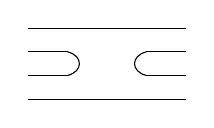
\begin{tikzpicture}
					\draw (0, 0) -- (2, 0);
					\draw (0, 0.3) -- (0.5, 0.3);
					\draw (0, 0.6) -- (0.5, 0.6);
					\draw (0.5, 0.3) .. controls (0.7, 0.35) and (0.7, 0.55) .. (0.5, 0.6);
					\draw (1.5, 0.3) -- (2, 0.3);
					\draw (1.5, 0.6) -- (2, 0.6);
					\draw (1.5, 0.3) .. controls (1.3, 0.35) and (1.3, 0.55) .. (1.5, 0.6);
					\draw (0, 0.9) -- (2, 0.9);
				\end{tikzpicture}
				\caption{Generator $U_2$ in TL$_4(\delta)$.}
				\label{fig:generator_temperley_lieb}
			\end{subfigure}
        	\end{figure}
        }
        
	\newdef{Frobenius algebra}{\index{Frobenius!algebra}
		An algebra $A$ equipped with a nondegenerate bilinear form $\eta:A\times A\rightarrow A$ satisfying the following condition for all $a,b,c\in A$:
		\begin{gather}
			\eta(ab,c)=\eta(a,bc)
		\end{gather}
	}

\subsection{Graded vector spaces}\label{section:graded_spaces}

	Similar to definition \ref{group:graded_ring} we can define the following:
	\newdef{Graded vector space}{\index{degree}\index{graded!vector space}
		Let $V_n$ be a vector space for all $n\in\mathbb{N}$. The vector space
		\begin{gather}
			\label{linalgebra:graded_vector_space}
			V = \bigoplus_{n\in\mathbb{N}} V_n
		\end{gather}
		is called a graded vector space. In fact one can replace $\mathbb{N}$ by any countable (finite or infinite) index set. For most operations however one requires the index set to be closed under addition operations. The index $n$ is often called the \textbf{degree} of the subspace $V_n$ in $V$.
	}
	
	\newdef{Graded algebra}{\index{graded!algebra}
		Let $V$ be a graded vector space with the additional structure of an algebra given by the multiplication $\star$. Then $V$ is a graded algebra if $\star$ maps $V^k\times V^l$ to $V^{k+l}$.
	}
	
	\newdef{Super vector space}{\index{super!vector space}
		A super vector space is defined as a $\mathbb{Z}_2$-graded vector space.
	}
	
	\begin{example}[Superalgebra]\index{super!algebra}\label{linalgebra:superalgebra}
		A $\mathbb{Z}_2$-graded algebra, i.e. there exists a decomposition
		\begin{gather}
			A = A_0\oplus A_1
		\end{gather}
		such that for all $i, j \mod 2$:
		\begin{gather}
			A_i\star A_j \subseteq A_{i+j}
		\end{gather}
	\end{example}
	
	\newdef{dg-algebra}{\index{dg-algebra}\label{linalgebra:dg_algebra}
		A differential graded algebra (often denoted by dg-algebra) is a graded algebra equipped with a differential of degree 1.
	}
	
	\newdef{Parity functor}{\index{parity}
		Consider the category $\mathbf{sVect}$ of super vector spaces. We can define the parity functor $\func{\Pi}{sVect}{sVect}$ as the functor which interchanges even and odd subspaces:
		\begin{align}
			(\Pi V)_0 &= V_1\\
			&\\
			(\Pi V)_1 &= V_0
		\end{align}
	}
	\newdef{Symmetric tensors}{
		Using the parity functor one can write the exterior algebra $\Lambda^\bullet(V)$ as the symmetric algebra $\text{Sym}^\bullet(\Pi V)$. In a similar way one can write the symmetric algebra on a super vector space $V=V_0\oplus V_1$ as $\text{Sym}^n(V)=\bigoplus_{p+q=n}\text{Sym}^p(V_0)\otimes\Lambda^q(V_1)$.
	}
        
\section[Linear maps]{Linear maps\footnote{Other names are \textbf{linear mapping} and \textbf{linear transformation}.}}
	
	\begin{property}
		Let $V$ be finite-dimensional $K$-vector space. Let $f:V\rightarrow V$ be a linear map. The following statements are equivalent:
        	\begin{itemize}
            		\item $f$ is injective
			\item $f$ is surjective
                	\item $f$ is bijective
		\end{itemize}
	\end{property}

	\newdef{Automorphism}{\index{automorphism}\label{linalgebra:automorphism}
		\nomenclature[S_Aut]{$\text{Aut}(V)$}{Set of automorphisms (invertible endomorphisms) on a set $V$.}
	    	An isomorphism from $V$ to $V$ is called an automorphism\footnote{In some case also called a \textbf{linear operator}, but this terminology is also used for a general linear map in operator theory (see chapter \ref{chapter:operator:algebras}).}. The set of all automorphisms  on $V$, which is in fact a group, is denoted by $\text{Aut}(V)$.
	}
    
	\newdef{General linear group\footnotemark}{\index{general linear group}
		\nomenclature[S_GL]{GL$(V)$}{General linear group: group of all automorphisms on a vector space $V$.}
		\footnotetext{This group is isomorphic to the general linear group of invertible matrices, hence the similar name and notation. (See definition \ref{linalgebra:GL_matrices})}
	    	The set of all automorphisms $f:V\rightarrow V$ is called the general linear group and denoted by GL$_K(V)$ or GL$(V)$ when the base field is clear.
	}

	\newdef{Rank}{\index{rank}\label{linalgebra:image_rank}
		The dimension of the image of a linear map is called the rank.
	}
	\newdef{Kernel}{\index{kernel}
	        The kernel of a linear map $f: V \rightarrow W$ is defined as the following subspace of $V$:
        	\begin{gather}
        		\text{ker}(f) = \{v\in V\ |\ f(v) = 0\}
	        \end{gather}
	}
	\newdef{Nullity}{\index{nullity}
		The dimension of the kernel is called the nullity.
	}
    
	\begin{theorem}
	    	A linear map $f:V\rightarrow W$ is injective if and only if $\text{ker}(f) = \{0\}$.
	\end{theorem}
	\begin{property}
	        Let $f:V\rightarrow W$ be a linear map. Let $U\leq V$. We have the following two properties of the restriction $f|_U$ of $f$ to $U$:
        	\begin{itemize}
			\item $\text{ker}\left(f|_U\right) = \text{ker}(f)\cap U$
        		\item $\text{im}\left(f|_U\right) \leq \text{im}(f)$
		\end{itemize}
	\end{property}
    
\subsection{Dimension}

        \begin{theorem}[Dimension theorem\footnotemark]\index{rank-nullity theorem}
		\footnotetext{Also called the \textbf{rank-nullity theorem}.}
		Let $f: V \rightarrow W$ be a linear map.
	        \begin{gather}
	                \label{linalgebra:dimension_theorem}
	                \dim(\text{\upshape im}(f)) + \dim(\text{\upshape ker}(f)) = \dim(\text{\upshape V})
	        \end{gather}
        \end{theorem}

        \begin{property}
		Two $K$-vector spaces are isomorphic if and only if they have the same dimension.
	\end{property}
    
\subsection{Homomorphisms}

	\newdef{Homomorphism space}{\index{morphism!of vector spaces}
		\nomenclature[S_Hom]{$\hom(V, W)$}{Set of morphisms from a set $V$ to a set $W$.}
    		Let $V,W$ be two K-vector spaces. The set of all linear maps between $V$ and $W$ is called the homomorphism space of $V$ to $W$, or shorter: the 'hom-space' of $V$ to $W$.
	    	\begin{equation}
        		\label{linalgebra:hom_space}
        		\hom_K(V, W) = \{f:V\rightarrow W\ |\ \text{f is linear}\}
		\end{equation}
	}
	\begin{theorem}\label{linalgebra:hom_dimension}
	    	If $\ V,W$ are two finite-dimensional K-vector spaces we have:
        	\begin{equation}
        		\dim\left(\emph{Hom}_K(V,W)\right) =\dim(V)\cdot\dim(W)
		\end{equation}
	\end{theorem}
        
	\newdef{Endomorphism ring}{
		\nomenclature[S_End]{$\text{End}(V)$}{Ring of endomorphisms on a set $V$.}
		The space $\hom_K(V, V)$ with the composition as multiplication forms a ring, the endomorphism ring. It is denoted by $\text{End}_K(V)$ or $\text{End}(V)$.
	}
	\begin{property}
		The endomormphism ring $\text{End}(V)$ forms a Lie algebra\footnote{See also \ref{lie:end_as_lie_algebra}.} when equipped with the commutator $[A, B] = A\circ B - B\circ A$.
	\end{property}
	
	\begin{property}[Jordan-Chevalley decomposition]\index{Jordan!decomposition}\index{semisimple!operator}\index{nilpotent}\label{linalgebra:jordan_chevalley}
		Every endomorphism $A$ can be decomposed as follows:
		\begin{equation}
			A = A_{ss} + A_n
		\end{equation}
		where
		\begin{itemize}
			\item $A_{ss}$ is \textbf{semisimple}, i.e. for every the invariant subspace of $A_{ss}$ there exists an invariant complementary subspace.
			\item $A_n$ is \textbf{nilpotent}, i.e. $\exists k\in\mathbb{N}: A_n^k = 0$.
		\end{itemize}
		Furthermore, this decomposition is unique and the endomorphisms $A_{ss}, A_n$ can be written as polynomials in $A$.
	\end{property}
    
	\newdef{Minimal polynomial}{\index{minimal polynomial}
	    	Let $f\in\text{End}(V)$ and $V$ a finite-dimensional K-vector space. The monic polynomial $\mu_f(x)$ of the lowest order such that $\mu_f(f)=0$ is called the minimal polynomial of $f$.
	}
	\begin{property}\label{linalgebra:minimal_polynomial_divisor}
		Let $f\in\text{End}(V)$. Let $\mu_f(x)$ be the minimal polynomial of $f$. Let $\varphi(x)\in K[x]$. If $\varphi(f) = 0$, then the minimal polynomial $\mu_f(x)$ divides $\varphi(x)$. 
	\end{property}
    
\subsection{Dual space}

	\newdef{Dual space}{\index{dual!space}
	    	Let $V$ be a K-vector space. The dual space $V^*$ of $V$ is the following vector space:
	    	\begin{equation}
			\label{linalgebra:dual_space}
		        V^*:=\text{Hom}_K(V, K)=\{f:V\rightarrow K\ :\ f\text{ is a linear map}\}
		\end{equation}
	}
	\newdef{Linear form}{\index{linear!form}
	    	The elements of $V^*$ are called \textit{linear forms}.
	}
	\begin{property}\label{linalgebra:dual_space_dimension}
		From theorem \ref{linalgebra:hom_dimension} it follows that $\dim(V^*) = \dim(V)$.
	\end{property}
	\begin{remark}
		If $V$ is infinite-dimensional, theorem \ref{linalgebra:dual_space_dimension} is not valid. In the infinite-dimensional case we \textbf{always} have $|V^*|>|V|$ (where we now use the cardinality instead of the dimension).
	\end{remark}
    
	\newdef{Dual basis}{
    		Let $\mathcal{B} = \{e_1, e_2, ..., e_n\}$ be a basis for a finite-dimensional K-vector space $V$. We can define a basis $\mathcal{B}^* = \{\varepsilon_1, \varepsilon_2, ..., \varepsilon_n\}$ for $V^*$, called the dual basis of $\mathcal{B}$, as follows:
    		\begin{equation}
			\label{linalgebra:dual_basis}
        		\boxed{\varepsilon_i:V\rightarrow K:\sum_{j=1}^na_ie_i\mapsto a_i}
		\end{equation}
		The relation between the basis and dual basis can also be written as:
		\begin{equation}
			\label{linalgebra:dual_basis_2}
			\varepsilon^i(e_j) = \delta^i_j
		\end{equation}
	}
    
	\newdef{Dual map}{\index{dual!map}\label{linalgebra:transpose}
		Let $f:V\rightarrow W$ be a linear map. The linear map $f^*:W^*\rightarrow V^*:\varphi\rightarrow\varphi\circ f$ is called the dual map or \textbf{transpose} of $f$.
	}
	\newnot{Transpose}{\index{transpose}
		When $V=W$ the dual map $f^*$ is often denoted by $f^T$.
	}
    
    \newdef{Natural pairing}{\index{natural!pairing}
    	The natural pairing of $V$ and its dual $V^*$ is defined as the following bilinear map:
        \begin{equation}
        	\label{linalgebra:natural_pairing}
            \langle v, v^*\rangle = v^*(v)
        \end{equation}
    }

\subsection{Convex functions}
	
	\newdef{Convex function}{\index{convex!function}
		Let $X$ be a convex subset of $V$. A function $f:X\rightarrow \mathbb{R}$ is convex if for all $x, y\in X$ and $t\in[0, 1]$:
		\begin{equation}
			f(tx + (1-t)y) \leq tf(x) + (1-t)f(y)
		\end{equation}
	}
	\begin{remark}
		For a concave function we have to turn the inequality around.
	\end{remark}
	\begin{result}
		A linear map $f:X\rightarrow\mathbb{R}$ is both convex and concave.
	\end{result}
	
	\begin{theorem}[Karamata's inequality]\index{Karamata's inequality}
		Let $I\subset\mathbb{R}$ be an interval and let $f:I\rightarrow\mathbb{R}$ be a convex function. If $(x_1, ..., x_n)$ is a tuple that majorizes $(y_1, ..., y_n)$, i.e. $\forall k\leq n$
		\begin{align}
			\sum_{i=1}^nx_i &= \sum_{i=1}^ny_i\\
			x_{(1)} + ... + x_{(k)}&\geq y_{(1)} + ... + y_{(k)}
		\end{align}
		where $x_{(i)}$ denotes the ordering\footnote{In decreasing order: $x_{(1)}\geq...\geq x_{(n)}$.} of the tuple $(x_1, ..., x_n)$. Then
		\begin{equation}
			\sum_{i=1}^nf(x_i)\geq \sum_{i=1}^nf(y_i)
		\end{equation}
	\end{theorem}

\section{Inner product}\label{linalgebra:innerproduct}

    In this section all vector spaces $V$ will be defined over $\mathbb{R}$ or $\mathbb{C}$.

\subsection{Inner product space}

    \newdef{Inner product}{\index{inner!product}
        A map $\langle\cdot|\cdot\rangle:V\times V\rightarrow\mathbb{C}$ is called an inner product on $V$ if it satisfies the following properties for all $v,w\in V$ and $\lambda\in\mathbb{C}$:
        \begin{enumerate}
            \item \textbf{Conjugate symmetry}: $\langle v|w \rangle = \langle w|v \rangle^*$,
            \item \textbf{Linearity in the first argument}: $\langle \lambda u+v|w \rangle = \lambda\langle u|w \rangle + \langle v|w \rangle$,
            \item \textbf{Nondegeneracy}: $\langle v|v \rangle = 0 \iff v = 0$, and
            \item \textbf{Positive-definiteness}: $\langle v|v \rangle \geq 0$.
        \end{enumerate}
    }
    \begin{remark}\index{Hermitian!form}\label{linalgebra:NDH_form}
        Inner products are special cases of \textbf{nondegenerate Hermitian forms} which do not satisfy the positive-definiteness property (these often occur when working over $\mathbb{C}$).
    \end{remark}

    \begin{result}\index{sesquilinear}
        The first two properties have the result of conjugate linearity in the second argument:
        \begin{gather}
            \langle f|\lambda g + \mu h \rangle = \overline{\lambda}\langle f|g \rangle + \overline{\mu}\langle f|h \rangle
        \end{gather}
        Therefore these two properties together are often combined into a \textbf{sesquilinearity} property. When the underlying field is restricted to $\mathbb{R}$, such that the conjugate symmetry property is replaced by symmetry, the inner product becomes a bilinear form.
    \end{result}

    \newdef{Inner product space\footnotemark}{
        \footnotetext{Sometimes called a \textbf{pre-Hilbert space}.}
        A vector space equipped with an inner product $\langle\cdot|\cdot\rangle$.
    }

    \newdef{Metric dual\footnotemark}{
        \footnotetext{See also Definition \ref{riemann:flat_map}.}
        Using the inner product (or any other nondegenerate Hermitian form) one can define the metric dual of a vector $v$ by the following map:
        \begin{gather}
            \label{linalgebra:metric_dual}
            L:V\rightarrow V^*:v\mapsto \langle v|\cdot \rangle.
        \end{gather}
    }
    \newdef{Adjoint operator}{\index{adjoint}\index{Hermitian}\index{self-adjoint}\label{linalgebra:adjoint_operator}
        Let $A$ be a linear operator on $V$. The (\textbf{Hermitian}) adjoint of $A$ is defined as the linear operator $A^\dag$ that satisfies
        \begin{gather}
            \langle A^\dag v|w\rangle = \langle v|Aw\rangle
        \end{gather}
        for all $v,w\in V$. Alternatively, one can define the adjoint using the transpose and metric dual as follows:
        \begin{gather}
            A^\dag = L^{-1} \circ A^T \circ L.
        \end{gather}
        If $A=A^\dag$, then A is said to be \textbf{Hermitian} or \textbf{self-adjoint}. (In Chapter \ref{chapter:normed_spaces} a distinction will be made between these two notions.)
    }
    \begin{result}
        The Hermitian adjoint of a complex matrix $A\in\mathbb{C}^{m\times n}$ is given by
        \begin{gather}
            A^\dag = \overline{A}^T,
        \end{gather}
        where $\overline{A}$ denotes the complex conjugate of $A$ and $A^T$ the transpose of $A$.
    \end{result}

\subsection{Orthogonality}\label{linalgebra:section:orthogonality}

    \newdef{Orthogonal}{\index{orthogonal}\label{linalgebra:orthogonal}
        Consider two vectors $v,w\in V$ in an inner product space. These vectors are said to be orthogonal, denoted by $v\perp w$,  if they obey the following relation:
        \begin{gather}
            \langle v|w \rangle = 0.
        \end{gather}
        An \textbf{orthogonal system} is a collection of vectors, none of them equal to 0, that are mutually orthogonal.
    }
    \begin{property}
        Orthogonal systems are linearly independent.
    \end{property}

    \newdef{Orthonormal}{\index{orthonormal}\label{linalgebra:orthonormal}
        A collection of vectors $S$ is said to be orthonormal if it forms an orthogonal system and if all the elements $v\in S$ obey the following relation:
        \begin{gather}
            \langle v|v \rangle = 1.
        \end{gather}
    }
    \newdef{Orthogonal complement}{\index{complement}\label{linalgebra:orthogonal_complement}
        Let $W$ be a subspace of an inner product space $V$. The orthogonal complement of $W$ is defined as the following subspace:
        \begin{gather}
            W^\perp := \{v\in V\mid\forall w\in W:\langle v|w\rangle = 0\}.
        \end{gather}
    }
    \sremark{$W^\perp$ is pronounced as 'W-perp'.}

    \begin{property}[Complements]
        Let $V$ be a finite-dimensional inner product space. The orthogonal complement $W^\perp$ is a complementary subspace to $W$, i.e. $W\oplus W^\perp=V$.
    \end{property}
    \begin{result}\label{linalgebra:perp_of_perp}
        Let $W\leq V$ where $V$ is a finite-dimensional inner product vector space. Taking orthogonal complements defines an involution:
        \begin{gather}
            (W^\perp)^\perp = W.
        \end{gather}
    \end{result}

    \newdef{Orthogonal projection}{\index{projection}\label{linalgebra:orthogonal_projection}
        Let $V$ be a finite-dimensional inner product vector space and consider a subspace $W\leq V$. Consider a vector $w\in W$ and let $\{w_1, \ldots, w_k\}$ be an orthonormal basis of $W$. The projections of $v\in V$ on $W$ and $w\in W$ are defined as follows:
        \begin{align}
            \text{proj}_W(v) &:= \sum_{i=1}^k\langle v|w_i \rangle w_i\\
            \text{proj}_w(v) &:= \stylefrac{\langle v|w \rangle}{\langle w|w \rangle}w.
        \end{align}
    }
    \begin{property}
        Orthogonal projections satisfy the following conditions:
        \begin{itemize}
            \item $\forall w\in W:\text{proj}_W(w) = w$, and
            \item $\forall u\in W^\perp:\text{proj}_W(u) = 0$.
        \end{itemize}
    \end{property}

    \newmethod{Gram-Schmidt orthonormalization}{\label{linalgebra:inner_product:gram_schmidt}
        Let $\{u_i\}_{i\leq n}$ be a set of linearly independent vectors. An orthonormal set $\{e_i\}_{i\leq n}$ can be constructed out of $\{u_i\}_{i\leq n}$ using the following procedure:
        \begin{enumerate}
            \item Orthogonalization:
                \begin{gather}
                    \begin{aligned}
                        w_1& = u_1&\\
                        w_2& = u_2 - \stylefrac{\langle u_2|w_1\rangle}{||u_2||^2}w_1&\\
                        &\vdots&\\
                        w_n& = u_n - \sum_{i=1}^{n-1}\stylefrac{\langle u_n|w_i\rangle}{||u_n||^2}w_i&
                    \end{aligned}
                \end{gather}
            \item Normalization:
                \begin{gather}
                    \begin{aligned}
                        e_1& = \stylefrac{w_1}{||w_1||}&\\
                        e_2& = \stylefrac{w_2}{||w_2||}&\\
                        &\vdots&\\
                        e_n& = \stylefrac{w_n}{||w_n||}&
                    \end{aligned}
                \end{gather}
        \end{enumerate}
    }

    \newdef{Householder transformation}{\index{Householder transformation}\label{linalgebra:householder_transformation}
        Let $v$ be an element of an inner product space $V$. The Householder transformation generated by $v$ is given by the linear map
        \begin{gather}
            \sigma_v:V\rightarrow V:w\mapsto w - 2\frac{\langle w|v \rangle}{\langle v|v \rangle}v.
        \end{gather}
        This transformation amounts to a reflection in the hyperplane orthogonal to $v$.
    }

    \newdef{Angle}{\index{angle}\label{linalgebra:angle}
        Let $v,w$ be elements of an inner product space $V$. The angle $\theta$ between $v$ and $w$ is defined by the following formula:
        \begin{gather}
            \cos\theta := \stylefrac{\langle v|w \rangle}{||v||||w||}.
        \end{gather}
    }
\section{Matrices}
	
	\begin{notation}\label{linalgebra:matrix_set}
	        The set of all $m\times n$-matrices defined over the field $K$ is denoted by $M_{m,n}(K)$. If $m=n$, the set is denoted by $M_n(K)$.
	\end{notation}
	
	\begin{property}[Dimension]\index{dimension}\label{linalgebra:dimension_of_matrix_space}
		The dimension of $M_{m,n}(K)$ as a vector space is $mn$.
	\end{property}
    
	\newdef{Trace}{\index{trace}\label{linalgebra:trace}
	        Let $A = (a_{ij})\in M_n(K)$. We define the trace of $A$ as follows:
    		\begin{gather}
			\text{tr}(A) = \sum_{i=1}^na_{ii}
		\end{gather}
	}
	\begin{property}\label{linalgebra:trace_commutative}
		Let $A, B\in M_n(K)$. The trace satisfies the following properties:
	        \begin{enumerate}
        		\item $\text{tr}:M_n(K)\rightarrow K$ is a linear map
			\item $\text{tr}(AB) = \text{tr}(BA)$
			\item $\text{tr}(AB) \neq \text{tr}(A)\text{tr}(B)$
        		\item $\text{tr}(A^T) = \text{tr}(A)$
		\end{enumerate}
	\end{property}
    
	\newformula{Hilbert-Schmidt norm\footnotemark}{\index{Frobenius!norm}\index{Hilbert-Schmidt norm}
    		\footnotetext{Also called the \textbf{Frobenius norm}.}
    		The Hilbert-Schmidt norm is given by the following formula:
	        \begin{gather}
        		\label{linalgebra:hilbert_schmidt_norm}
        		||A||^2_{HS} = \sum_{i, j}|A_{ij}|^2 = \text{tr}(A^\dag A)
	        \end{gather}
        	If one identifies $M_{n}(\mathbb{C})$ with $\mathbb{C}^{2n}$ then this norm equals the standard Hermitian norm.
	}

	\newformula{Hadamard product}{\index{Hadamard!product}
    		The Hadamard product of two matrices $A, B\in M_{m\times n}(K)$ is defined as the entry-wise product:
        	\begin{gather}
        		(A\circ B)_{ij} = A_{ij}B_{ij}
        	\end{gather}
	}
    
	\newdef{General linear group}{\index{general linear group}\label{linalgebra:GL_matrices}
		\nomenclature[S_GLn]{GL$(n,K)$}{General linear group: group of all invertible $n$-dimensional matrices over the field $K$.}
	        The set of invertible matrices is called the general linear group and is denoted by GL$_n(K)$ or GL$(n, K)$.
	}
	\begin{property}
		For all $A\in\text{GL}_n(K)$ we have:
	        \begin{itemize}
			\item $A^T\in\text{GL}_n(K)$
		        \item $\left(A^T\right)^{-1}=\left(A^{-1}\right)^T$
		\end{itemize}
	\end{property}
    
	\begin{property}\label{linalgebra:dim_columns_rows}
		Let $A\in M_{m,n}(K)$. Denote the set of columns as $\{A_1, A_2, ..., A_n\}$ and the set of rows as $\{R_1, R_2, ..., R_m\}$. The set of columns is a subset of $K^m$ and the set of rows is a subset of $K^n$ and as such we can define their span. These spaces satisfy the following property:
		\begin{gather}
			\dim(\text{span}(A_1, ..., A_n)) = \dim(\text{span}(R_1, ..., R_m))
		\end{gather}
	\end{property}
	
	\newdef{Rank}{\index{rank}
		Using the invariance relation from previous property we can define the rank of a matrix $A\in M_{m,n}(K)$ as follows:
		\begin{gather}
			\label{linalgebra:matrix_rank}
        		\text{rk}(A) := \dim(\text{span}(A_1, ..., A_n)) \overset{\ref{linalgebra:dim_columns_rows}}{=} \dim(\text{span}(R_1, ..., R_m))
		\end{gather}
	}
    
	\begin{property}\label{linalgebra:rank_properties}
	        The rank of a matrix has the following properties:
        	\begin{enumerate}
			\item $\text{rk}(AC)\leq\text{rk}(A)$ and $\text{rk}(AC)\leq\text{rk}(C)$
        		\item $\text{rk}(BC)=\text{rk}(C)$
		        \item $\text{rk}(BD)=\text{rk}(D)$
		\end{enumerate}
		where $A\in M_{m,n}(K)$, $B\in\text{GL}_n(K)$, $C\in M_{n,r}(K)$ and $D\in M_{r,n}(K)$.
	\end{property}
	\begin{property}\label{linalgebra:dim_matrix_left_multiplication}
	        Let $A\in M_{m,n}(K)$. We first define the following linear map:
        	\begin{gather}
			\label{linalgebra:matrix_left_multiplication}
        		L_A:K^n\rightarrow K^m:v\mapsto Av
		\end{gather}
	        This map has the following properties:
        	\begin{enumerate}
        		\item $\text{im}(L_A) = \text{span}(A_1, ..., A_n)$
			\item $\dim(\text{im}(L_A))=\text{rk}(A)$
		\end{enumerate}
	\end{property}
	\sremark{The second property is a direct consequence of the first one together with definition \ref{linalgebra:matrix_rank}.}
    
\subsection{System of equations}

	\begin{property}\label{linalgebra:matrix_and_equations}
	        Let $AX=w$ with $A\in M_{m,n}(K)$, $w\in K^m$ and $X\in K^n$ be a system of $m$ equations in $n$ variables. Let $L_A$ be the linear map as defined in equation \ref{linalgebra:matrix_left_multiplication}. We then have the following properties:
        	\begin{enumerate}
			\item The system is false if and only if $w\not\in\text{im}(L_A)$.
        		\item If the system is not false, the solution set is an affine space. If $v_0\in K^n$ is a solution, then the solution set is given by: $L_A^{-1}(w)=v_0+\text{ker}(L_A)$.
		        \item If the system is homogeneous ($AX=0$), then the solution set is equal to $\text{ker}(L_A)$.
		\end{enumerate}
	\end{property}
	\begin{property}[Uniqueness]\label{linalgebra:rank_unique_solution}
	        Let $AX=w$ with $A\in M_n(K)$ be a system of $n$ equations in $n$ variables. If $\text{rk}(A)=n$, then the system has a unique solution.
	\end{property}
	
	\newformula{Cramer's rule}{\index{Cramer}
    		Let $AX = w$ be a system of linear equations where the matrix $A$ has a nonzero determinant. Then Cramer's rule gives a unique solution where the unknowns are given by;
		\begin{gather}
			\label{linalgebra:cramers_rule}
			X_i = \stylefrac{\det(A_i)}{\det(A)}
		\end{gather}
		where $A_i$ is the matrix obtained by replacing the $i^{th}$ column of $A$ by the column matrix $w$.
	}
    
\subsection{Coordinates and matrix representations}

        \newdef{Coordinate vector}{\label{linalgebra:coordinate_vector}
        	Let $\mathcal{B} = \{b_1, ..., b_n\}$ be a basis of $V$. Let $v\in V$ such that $v=\sum_{i=1}^n\lambda_ib_i$. We define the coordinate vector of $v$ with respect to $\mathcal{B}$ as $(\lambda_1, ..., \lambda_n)^T$. The $\lambda_i$'s are called the \textbf{coordinates} of $v$ with respect to $\mathcal{B}$.
        }
        \newdef{Coordinate isomorphism}{\label{linalgebra:coordinate_isomorphism}
        	With the previous definition in mind we can define the coordinate isomorphism of $v$ with respect to $\mathcal{B}$ as follows:
        	\begin{gather}
			\boxed{\beta:V\rightarrow K^n:\sum_{i=1}^n\lambda_ib_i\mapsto(\lambda_1, ..., \lambda_n)^T}
		\end{gather}
        }
        
        \newdef{Matrix representation}{\label{linalgebra:matrix_representation}
        	Let $V$ be an $n$-dimensional K-vector space and $W$ an $m$-dimensional K-vector space. Let $f:V\rightarrow W$ be a linear map. Let $\mathcal{B}=\{b_1, ..., b_n\}, \mathcal{C} = \{c_1, ..., c_m\}$ be a basis for $V$, respectively $W$. The matrix representation of $f$ with respect to $\mathcal{B}$ and $\mathcal{C}$ can be derived as follows: For every $j\in\{1, ..., n\}$ we can write $f(b_j) = \sum_{i=1}^ma_{ij}c_i$, so with this in mind we can define the matrix $(a_{ij})\in M_{m,n}(K)$ as the matrix represenation of $f$.
        }
        \newnot{Matrix representation of a linear map}{
        	The matrix representation of $f$ with respect to $\mathcal{B}$ and $\mathcal{C}$ is denoted by $A_{f, \mathcal{B}, \mathcal{C}}$.
        }
        
        \newmethod{Construction of a matrix representation}{\label{linalgebra:method:matrix_representation}
        	From definition \ref{linalgebra:matrix_representation} we can see that $j$-th column of $A_{f, \mathcal{B}, \mathcal{C}}$ coincides with the coordinate vector of $f(b_j)$ with respect to $\mathcal{C}$. We use this relation to construct $A_{f, \mathcal{B}, \mathcal{C}}$ by writing for every $j\in\{1, ..., n\}$ the coordinate vector of $f(b_j)$ in the $j$-th column.
        }
        
        \begin{theorem}\label{linalgebra:theorem:matrix_representation}
		Let $(\lambda_1, ..., \lambda_n)^T$ be the coordinate vector of $v\in V$ with respect to $\mathcal{B}$. Let $(\mu_1, ..., \mu_m)^T$ be the coordinate vector of $f(v)$ with respect to $\mathcal{C}$. Then the following relation holds:
            	\begin{gather}
			\left(
			\begin{array}{c}
				\mu_1\\
				\vdots\\
				\mu_m
			\end{array}\right)
	                = A_{f, \mathcal{B}, \mathcal{C}}
        	        \left(\begin{array}{c}
				\lambda_1\\
				\vdots\\
				\lambda_n
			\end{array}\right)
		\end{gather}
	\end{theorem}
        
        \begin{theorem}\label{linalgebra:theorem:map_matrix_link}
		For every matrix $A\in M_{m,n}(K)$ there exists a linear map $f:V\rightarrow W$ such that $A_{f, \mathcal{B}, \mathcal{C}} = A$.
	\end{theorem}
        On the other hand we also have the following theorem:
        \begin{theorem}
		Let $f:K^n\rightarrow K^m$ be a linear map. There exists a matrix $A\in M_{m,n}(K)$ such that $f=L_A$.
	\end{theorem}
        \begin{theorem}
		Let $\beta$ and $\gamma$ be the coordinate isomorphisms with respect to respectively $\mathcal{B}$ and $\mathcal{C}$. From theorem \ref{linalgebra:theorem:matrix_representation} it follows that:
        	\begin{gather}
			\gamma(f(v)) = A_f\cdot\beta(v)
		\end{gather}
        	or alternatively
        	\begin{gather}
			\gamma\circ f = L_{A_f}\circ\beta
		\end{gather}
	\end{theorem}
        
        \begin{theorem}\label{linalgebra:theorem:matrix_composition_hom}
	        The map $\text{Hom}_K(V,W)\rightarrow M_{m,n}(K):f\mapsto A_f$ is an isomorphism and for every $f\in\text{Hom}_K(V,W)$ and $g\in \text{Hom}_K(W,U)$ we have:
		\begin{gather}
			A_{g\circ f} = A_gA_f
		\end{gather}
	\end{theorem}
	
	\begin{theorem}\label{linalgebra:theorem:matrix_composition_end}
	        The map $\text{End}_K(V)\rightarrow M_n(K):f\mapsto A_{f, \mathcal{B}, \mathcal{B}}$ is an isomorphism and for every $f,g\in\text{End}_K(V)$ we have:
        	\begin{gather}
			A_{g\circ f} = A_gA_f
		\end{gather}
	\end{theorem}
	
        \begin{theorem}\label{linalgebra:matrix_invertable_map}
	        Let $f\in\text{End}_K(V)$. Let $A_f$ be the corresponding matrix representation. The linear map $f$ is invertible if and only if $A_f$ is invertible. Furthermore, if $A_f$ is invertible, we have that \[\left(A_f\right)^{-1} = A_{f^{-1}}\] In other words, the following map is an isomorphism\footnotemark:
	        \begin{gather}
	        	\text{GL}_K(V)\rightarrow\text{GL}_n(K):f\mapsto A_f
	        \end{gather}
	        \footnotetext{Follows from theorem \ref{linalgebra:theorem:matrix_composition_end}.}
	\end{theorem}
        \remark{The sets GL$_K(V)$ and GL$_N(K)$ are groups. So the previous theorem states that the map $f\mapsto A_f$ is a group isomorphism.}
        
        \begin{theorem}
		Let $V = K^n$. Let $f\in V^*$. From construction \ref{linalgebra:method:matrix_representation} it follows that $A_f = (f(e_1), ..., f(e_n))\in M_{1,n}(K)$ with respect to the standard basis of $V$. This combined with theorem \ref{linalgebra:theorem:matrix_representation} gives:
	        \begin{gather}
			f(\lambda_1, ..., \lambda_n)^T = (f(e_1), ..., f(e_n))(\lambda_1, ..., \lambda_n)^T = \sum_{i=1}^nf(e_i)\lambda_i
		\end{gather}
        	or alternatively with $\{\varepsilon_1, ..., \varepsilon_n\}$ the dual basis to the standard basis of $V$:
	        \begin{gather}
        	    	\label{linalgebra:map_in_function_of_dual_basis}
			\boxed{f = \sum_{i=1}^nf(e_i)\varepsilon_i}
		\end{gather}
	\end{theorem}
        
        \begin{theorem}
		Let $f:V\rightarrow W$ be a linear map. Let $f^*:W^*\rightarrow V^*$ be the corresponding dual map. If $A_f$ is the matrix representation of $f$ with respect to $\mathcal{B}$ and $\mathcal{C}$, then the transpose $A_f^T$ is the matrix representation of $f^*$ with respect to the dual basis of $\mathcal{C}$ and the dual basis of $\mathcal{B}$.
	\end{theorem}
        
\subsection{Coordinate transforms}
        
        \newdef{Transition matrix}{\label{linalgebra:transition_matrix}
        	Let $\mathcal{B} = \{b_1, ..., b_n\}$ and $\mathcal{B}' = \{b_1', ..., b_n'\}$ be two bases of $V$. Every element of $\mathcal{B}'$ can be written as a linear combination of elements in $\mathcal{B}$:
        	\begin{gather}
        		b_j' = q_{1j}b_1 + ... + q_{nj}b_n
        	\end{gather}
	        The matrix $Q = (q_{ij})\in M_n(K)$ is called the transition matrix from the 'old' basis $\mathcal{B}$ to the 'new' basis $\mathcal{B}'$.}
        
        \begin{theorem}\label{linalgebra:theorem:transition_matrix}
		Let $\mathcal{B}, \mathcal{B}'$ be two basis of $V$. Let $Q$ be the transition matrix from $\mathcal{B}$ to $\mathcal{B}'$. We find the following statements:
	        \begin{enumerate}
			\item Let $\mathcal{C}$ be an arbitrary basis of $V$ with $\gamma$ the corresponding coordinate isomorphism. Define the following matrices:
        	        	\[
        	        		B=(\gamma(b_1), ..., \gamma(b_n))\quad\text{and}\quad B'=(\gamma(b_1'), ..., \gamma(b_n'))
        	        	\]
		                Then $BQ = B'$.
			\item $Q\in\text{GL}_n(K)$ and $Q^{-1}$ is the transition matrix from $\mathcal{B}'$ to $\mathcal{B}$.
                	\item Let $v\in V$ with $(\lambda_1, ..., \lambda_n)^T$ the coordinate vector with respect to $\mathcal{B}$ and $(\lambda_1', ..., \lambda_n')^T$ the coordinate vector with respect to $\mathcal{B}'$. Then:
                	\[
		                Q\left(
				\begin{array}{c}
					\lambda_1'\\
                			\vdots\\
			        	\lambda_n'
				\end{array}
                        	\right)
                        	=
		                \left(
                		\begin{array}{c}
					\lambda_1\\
                			\vdots\\
			        	\lambda_n
				\end{array}
                        	\right)
				\quad\text{and}\quad
                        	\left(
                        	\begin{array}{c}
					\lambda_1'\\
                        		\vdots\\
			        	\lambda_n'
				\end{array}
		                \right)
                	        =
                	        Q^{-1}\left(
                	        \begin{array}{c}
					\lambda_1\\
                		        \vdots\\
			                \lambda_n
				\end{array}
                        	\right)
			\]
		\end{enumerate}
	\end{theorem}
        
	\begin{theorem}\label{linalgebra:theorem:transition_matrix_representation}
        	Let $V,W$ be two finite-dimensional K-vector spaces. Let $\mathcal{B}, \mathcal{B}'$ be two bases of $V$ and $\mathcal{C}, \mathcal{C}'$ two bases of $W$. Let $Q, P$ be the transition matrices from $\mathcal{B}$ to $\mathcal{B}'$ and from $\mathcal{C}$ to $\mathcal{C}'$ respectively. Let $A=A_{f, \mathcal{B}, \mathcal{C}}$ and $A' = A_{f, \mathcal{B}', \mathcal{C}'}$. Then:
	        \begin{gather}
        	    	A' = P^{-1}AQ
        	\end{gather}
	\end{theorem}
        \begin{result}
		Let $f\in \text{End}_K(V)$ and let $Q$ be the transition matrix. From theorem \ref{linalgebra:theorem:transition_matrix_representation} it follows that:
            	\begin{gather}
	            	A'=Q^{-1}AQ
        	\end{gather}
	\end{result}

        \newdef{Matrix conjugation}{\index{conjugacy class}\index{matrix!conjugation}\label{linalgebra:conjugacy_class}
        	Let $A\in M_n(K)$. The set
        	\begin{gather}
	            	\{Q^{-1}AQ\ |\ Q\in\text{GL}_n(K)\}
        	\end{gather}
	        is called the conjugacy class\footnotemark\ of $A$. Another name for conjugation is \textbf{similarity transformation}.
        	\footnotetext{This is the general definition of conjugacy classes for groups. Furthermore, these classes induce a partitioning of the group.}
	}
        \begin{remark}
        	If $A$ is a matrix representation of a linear operator $f$, then the conjugacy class of $A$ consists out of every possible matrix representation of $f$.
        \end{remark}
        
        \begin{property}
        	From property \ref{linalgebra:trace_commutative} it follows that the trace of a matrix is invariant under similarity transformations:
        	\begin{gather}
            		\label{linalgebra:trace_invariance}
            		\boxed{\text{tr}(Q^{-1}AQ) = \text{tr}(A)}
	        \end{gather}
        \end{property}
        
        \newdef{Matrix congruence}{\index{matrix!congruence}\label{linalgebra:matrix_congruence}
        	Let $A, B\in M_n(K)$. If there exists a matrix $P$ such that
	        \begin{gather}
        	    	A = P^TBP
        	\end{gather}
	        then the matrices are said to be congruent.
        }
        \begin{property}
        	Every matrix congruent to a symmetric matrix is also symmetric.
        \end{property}
        
        \begin{theorem}\label{linalgebra:theorem:orthogonal_transition_matrix}
        	Let $(V, \langle .|. \rangle)$ be an inner-product space defined over $\mathbb{R}$ (or $\mathbb{C}$). Let $\mathcal{B}, \mathcal{B}'$ be two orthonormal bases of $V$ and let $Q$ be the transition matrix. Then $Q$ is orthogonal:
        	\begin{gather}
	        	Q^TQ = \mathbbm{1}_n
	        \end{gather}
	\end{theorem}

\subsection{Determinant}

    	\newdef{Minor}{
        	The $(i, j)$-th minor of $A$ is defined as:\[\det(A_{ij})\] where $A_{ij}\in M_{n-1}(K)$ is the matrix obtained by removing the $i$-th row and the $j$-th column from $A$.
	}
        \newdef{Cofactor}{
        	The cofactor $\alpha_{ij}$ of the matrix element $a_{ij}$ is equal to:\[(-1)^{i+j}\det(A_{ij})\]where $\det(A_{ij})$ is the minor as previously defined.
	}
        \newdef{Adjugate matrix}{\label{linalgebra:adjugate_matrix}
	        The adjugate matrix of $A\in M_n(K)$ is defined as follows:
	       	\begin{gather}
	            	\text{adj}(A) := \left(
	                \begin{array}{cccc}
				\alpha_{11}&\alpha_{21}&\dotsm&\alpha_{n1}\\
		                \alpha_{12}&\alpha_{22}&\dotsm&\alpha_{n2}\\
		                \vdots&\vdots&\vdots&\vdots\\
		                \alpha_{1n}&\alpha_{2n}&\dotsm&\alpha_{nn}\\
			\end{array}
        	        \right)
		\end{gather}
        	or shorter: $\text{adj}(A) = (\alpha_{ij})^T$.
        }
        \begin{remark*}
		It is important to notice that we have to transpose the matrix after the elements have been replaced by their cofactor.
	\end{remark*}
        
        \begin{property}\label{linalgebra:determinant_properties}
	        Let $A,B\in M_n(K)$. Denote the columns of $A$ as $A_1, \dotso, A_n$. We have the following properties of the determinant:
	        \begin{enumerate}
			\item $\det(A^T) = \det(A)$
	                \item $\det(AB) = \det(BA) = \det(A)\det(B)$
	                \item $\det(A_1, \dotso, A_i+\lambda A_i', \dotso, A_n) = \det(A_1, \dotso, A_i, \dotso, A_n) + \lambda\det(A_1, \dotso,A_i', \dotso, A_n)$ for all $A_i,A_i'\in M_{n,1}(K)$.
	                \item If two columns of $A$ are equal then $\det(A) = 0$.
	                \item $\det(A_{\sigma(1)},\dotso,A_{\sigma(n)}) = \text{sgn}(\sigma)\det(A_1,\dotso,A_n)$
	                \item The determinant can be evaluated as follows:
	                	\begin{gather}
					\det(A) = \sum_{i=1}^n(-1)^{i+k}a_{ik}\det(A_{ik})
				\end{gather}
		\end{enumerate}
		\end{property}
        
	\begin{theorem}\label{linalgebra:theorem:rank_det_equivalence}
        	Let $A\in M_n(K)$, the following statements are equivalent:
        	\begin{enumerate}
			\item $\det(A) \neq 0$
        	        \item $\text{rk}(A) = n$
        	        \item $A\in\text{GL}_n(K)$
		\end{enumerate}
	\end{theorem}
        \begin{theorem}\label{linalgebra:theorem:adjugate_matrix}
            For all $A\in M_n(K)$ we find $A\text{adj}(A) = \text{adj}(A)A = \det(A)I_n$.
	\end{theorem}
        \begin{formula}\label{linalgebra:theorem:determinant_inverse}
	        For all $A\in\text{GL}_n(K)$ we find:
		\begin{gather}
            		A^{-1} = \det(A)^{-1}\ \text{adj}(A)
            	\end{gather}
	\end{formula}
        
        An alternative definition of a $k\times k$-minor is: 
        \begin{definition}
		Let $A\in M_{m,n}(K)$ and $k\leq\min(m, n)$. A $k\times k$-minor of $A$ is the determinant of a $k\times k$-partial matrix obtained by removing $m-k$ rows and $n-k$ columns from $A$.
	\end{definition}
        \begin{theorem}
		Let $A\in M_{m,n}(K)$ and $k\leq\min(m, n)$. We find that $\text{rk}(A)\geq k$ if and only if $A$ contains a non-zero $k\times k$-minor.
	\end{theorem}
        
        \begin{theorem}
		Let $f\in\textup{End}_K(V)$. The determinant of the matrix representation of $f$ is invariant under basis transformations.
	\end{theorem}
	
        \newdef{Determinant of a linear operator}{\index{determinant}\label{linalgebra:operator_determinant}
        	The previous theorem allows us to unambiguously define the determinant of $f\in\textup{End}_K(V)$ as follows:
        	\[\det(f) := \det(A)\]
		where $A$ is some matrix representation of $f$.
        }

\subsection{Characteristic polynomial}

    	\begin{definition}[Characteristic polynomial\footnotemark]\index{characteristic!polynomial}\label{linalgebra:characteristic_polynomial}
		Let $V$ be a finite-dimensional K-vector space. Let $f\in \text{End}_K(V)$ be a linear operator with the matrix representation $A$ (with respect to some arbitrary basis). We then find:
		\begin{gather}
                	\chi_f(x) := \det(x\mathbbm{1}_n - A) \in K[x]
		\end{gather}
		is a monic polynomial of degree $n$ in the variable $x$ and the polynomial does not depend on the choice of basis.
		\footnotetext{This polynomial can also be used directly for a matrix $A$ as theorem \ref{linalgebra:theorem:map_matrix_link} matches every matrix $A$ with some linear operator $f$.}
	\end{definition}
        
        \begin{definition}[Characteristic equation\footnotemark]\index{characteristic!equation}
        	\footnotetext{This equation is sometimes called the \textbf{secular equation}.}
		The following equation is called the characteristic equation of $f$:
	        \begin{gather}
            		\label{linalgebra:characteristic_equation}
			\boxed{\chi_f(x) = 0}
		\end{gather}
	\end{definition}
        
        \begin{formula}\label{linalgebra:parts_of_characteristic_polynomial}
        	Let $A=(a_{ij})\in M_n(K)$ with characteristic polynomial: \[\chi_A(x) = x^n + c_{n-1}x^{n-1} + \dotso + c_1x + c_0\] We then have the following result:
        	\begin{gather}
			\begin{cases}
				c_0 = (-1)^n\det(A)\\
				c_{n-1} = -\text{tr}(A)
			\end{cases}
		\end{gather}
	\end{formula}
        
        \begin{theorem}[Cayley-Hamilton]\index{Cayley-Hamilton theorem}\label{linalgebra:cayley_hamilton}\
	        \begin{enumerate}
			\item Let $A\in\text{M}_n(K)$ with characteristic polynomial $\chi_A(x)$. We find the following relation:
		                \begin{gather}
					\chi_A(A) = A^n + \sum_{i=1}^{n-1}c_iA^i= 0
				\end{gather}
	                \item Let $f\in\textup{End}_K(V)$ with characteristic polynomial $\chi_f(x)$. We find that
		                \begin{gather}
					\chi_f(f) = f^n + \sum_{i=1}^{n-1}c_if^i= 0
				\end{gather}
		\end{enumerate}
	\end{theorem}
        \begin{result}
		From theorem \ref{linalgebra:minimal_polynomial_divisor} and the Cayley-Hamilton theorem it follows that the minimal polynomial $\mu_f(x)$ is a divisor of the characteristic polynomial $\chi_f(x)$.
	\end{result}
        
\subsection{Linear groups}\label{linalgebra:section:linear_groups}
        
        \newdef{Elementary matrix}{\label{linalgebra:elementary_matrix}An elementary matrix is a matrix of the following form:
        	\[\left(
                \begin{array}{cccc}
			1&0&\dotsm&0\\
        	        0&1&c_{ij}&0\\
                	\vdots&\vdots&\ddots&\vdots\\
	                0&0&\vdots&1
		\end{array}
		\right),
        	\left(
                \begin{array}{cccc}
			1&0&\dotsm&0\\
                	0&1&\dotsm&0\\
	                \vdots&c_{ij}&\ddots&\vdots\\
        	        0&0&\vdots&1
		\end{array}
		\right),\dotso\]
		i.e. equal to the sum of an identity matrix and a multiple of a matrix unit $U_{ij}, i\neq j$.
        }
        \newnot{Elementary matrix}{$E_{ij}(c)$ is the elementary matrix with element $c$ on the $i,j$-th position.}
        \begin{property}
        	We have the following property:
		\begin{gather}
			\det(E_{ij}(c)) = 1
		\end{gather}
		which implies that $E_{ij}(c)\in\text{GL}_n(K)$.
	\end{property}
        \begin{property}
		We find the following results concerning the multiplication by an elementary matrix:
	        \begin{enumerate}
			\item Left multiplication by an elementary matrix $E_{ij}(c)$ comes down to replacing the $i$-th row of the matrix with the $i$-th row plus $c$ times the $j$-th row.
                	\item Right multiplication by an elementary matrix $E_{ij}(c)$ comes down to replacing the $j$-th column of the matrix with the $j$-th column plus $c$ times the $i$-th column.
		\end{enumerate}
		\end{property}
        
        \begin{theorem}\label{linalgebra:theorem:elementary_matrices}
		Every matrix $A\in\text{GL}_n(K)$ can be written in the following way: \[A = SD\] where $S$ is a product of elementary matrices and $D=\text{diag}(1,\dotso,1,\det(A))$.
	\end{theorem}
        
        \newdef{Special linear group}{\label{linalgebra:special_linear_group}
        	The following subset of GL$_n(K)$ is called the special linear group:
		\begin{gather}
			\text{SL}_n(K) = \{A\in \text{GL}_n(K)\ |\ \det(A) = 1\}
		\end{gather}
        }
        \begin{theorem}
		Every $A\in\text{SL}_n(K)$ can be written as a product of elementary matrices.\footnote{This follows readily from theorem \ref{linalgebra:theorem:elementary_matrices}.}
	\end{theorem}
        
        \newdef{Orthogonal group}{\label{linalgebra:orthogonal_group}The orthogonal and special orthogonal group are defined as follows:
        	\begin{align}
			\text{O}_n(K) &= \{A\in \text{GL}_n(K)\ |\ AA^T = A^TA = I_n\}\nonumber\\
			\text{SO}_n(K) &= \text{O}_n(K)\cap \text{SL}_n(K)\nonumber
		\end{align}
        }
        \begin{property}\label{linalgebra:con_equivalence}
        	For orthogonal matrices, conjugacy \ref{linalgebra:conjugacy_class} and congruency \ref{linalgebra:matrix_congruence} are equivalent.
        \end{property}
        
        \newdef{Unitary group}{\label{linalgebra:unitary_group}\index{involution}
        	The unitary and special unitary group are defined as follows:
        	\begin{align}
			\text{U}_n(K, \sigma) &= \{A\in \text{GL}_n(K)\ |\ A\overline{A}^T = \overline{A}^TA = I_n\}\nonumber\\
			\text{SU}_n(K, \sigma) &= \text{U}_n(K)\cap \text{SL}_n(K)\nonumber
		\end{align}
		where $\sigma$ denotes the \textit{involution}\footnotemark\ $a^\sigma \equiv \overline{a}$.
		\footnotetext{An involution is an operator that is its own inverse: $f(f(x)) = x$.}
        }

	\begin{remark*}
		If $K=\mathbb{C}$ where the involution is taken to be the complex conjugate, the $\sigma$ is often ommited in the definition: U$_n(K)$ and SU$_n(K)$.
	\end{remark*}
	
	\newdef{Unitary equivalence}{
		Let $A, B$ be two matrices in M$_n(K)$. If there is a unitary matrix $U$ such that \[A = U^\dag BU\] then the matrices $A$ and $B$ are said to be \textbf{unitarily equivalent}.
	}
	
	\newdef{Symplectic group}{\index{symplectic!group}
		\nomenclature[S_SymA]{Sp$_n(K)$}{Symplectic group: Group of matrices preserving the canonical symplectic form over the field $K$.}
		Consider a vector space $V$ with an antisymmetric nonsingular matrix $\Omega$. The symplectic group Sp$_n(V, \Omega)$ is defined as follows:
		\begin{gather}
			\label{linalgebra:symplectic_group}
			\text{Sp}(V, \Omega) = \{A\in\text{GL}(V)\ |A^T\Omega A = \Omega\}.
		\end{gather}
		On the real or complex numbers one can define the canonical \textbf{symplectic} matrix \[\Omega_{st} = \begin{pmatrix}0&-\mathbbm{1}\\\mathbbm{1}&0\end{pmatrix}\]
		The group of matrices that preserve this matrix are often denoted by Sp$_n(\mathbb{R})$ or Sp$_n(\mathbb{C})$.
	}
	\begin{property}
		Symplectic groups can only be defined on even-dimensional spaces because the defining matrix $\Omega$ can only be nonsingular if $n$ is even.
	\end{property}
	
	\newdef{Compact symplectic group}{
		\nomenclature[S_SymC]{Sp$(n)$}{Compact symplectic group: Sp$_{2n}(\mathbb{C})\cap\text{U}(2n)$.}
		The compact symplectic group is defined as follows:
		\begin{gather}
			\text{Sp}(n) = \text{Sp}_{2n}(\mathbb{C})\cap\text{U}(2n).
		\end{gather}
		This is in fact isomorphic to the \textit{quaternionic unitary group} in $n$ quaternionic dimensions.
	}
	\begin{example}
		For $n=1$ we find Sp$(1)\cong\text{SU}(2)$.
	\end{example}
	
\subsection{Matrix decomposition}

	\begin{method}[QR Decomposition]\index{QR!decompositon}
		Every square complex matrix $M$ can be decomposed as
		\begin{gather}
			M = QR
		\end{gather}
		where $Q$ is unitary and $R$ is upper-triangular. The easiest (but not the most numerically stable) way to do this is by applying the Gram-Schmidt orthonormalisation process:
		
		Let $\{v_i\}_{i\leq n}$ be a basis for the column space of $M$. By applying the Gram-Schmidt process to this basis one obtains a new orthonormal basis $\{e_i\}_{i\leq n}$. The matrix $M$ can then be written as $QR$ where:
		\begin{itemize}
			\item $R$ is an upper-triangular matrix with entries $R_{ij} = \langle e_i|\text{col}_j(M) \rangle$ where col$_j(M)$ denotes the $j^{th}$ column of $M$.
			\item $Q = (a_1\cdots a_n)$ is the unitary matrix constructed by setting the $i^{th}$ column equal to the $i^{th}$ basis vector $a_i$ 
		\end{itemize}
	\end{method}
	\begin{property}
		If $M$ is invertible and if the diagonal elements of $R$ are required to have positive norm then the QR-decomposition is unique.
	\end{property}

\section{Eigenvectors}

    \begin{definition}[Eigenvector]\index{eigenvalue}\index{eigenvector}
        A vector $v\in V\setminus\{0\}$ is called an \textbf{eigenvector} of the linear map $f:V\rightarrow V$ if it satisfies
       \begin{gather}
            f(v) = \lambda v
        \end{gather}
       for some $\lambda\in K$. The scalar $\lambda$ is called the \textbf{eigenvalue} associated to $v$.
    \end{definition}
    \begin{definition}[Eigenspace]\label{linalgebra:eigenvalue_remark}
        The subspace of $V$ spanned by the eigenvectors of a linear map is called the eigenspace of that linear map. It is given by
        \begin{gather}
            \ker(\lambda\mathbbm{1}_V - f).
        \end{gather}
        It follows that the eigenvalues are exactly those scalars for which the linear map $\lambda\mathbbm{1}_V-f$ is not injective. (This is generalized in Section \ref{section:spectrum}.)
    \end{definition}

    \begin{property}[Characteristic equation]\index{characteristic!equation}\label{linalgebra:eigenvalue_characteristic_equation}
        Consider a linear map $f\in\End(V)$. A scalar $\lambda\in K$ is an eigenvalue of $f$ if and only if it satisfies the characteristic equation \ref{linalgebra:characteristic_equation}.
    \end{property}
    \begin{property}
        A linear map $f\in\End(V)$ defined over an $n$-dimensional vector space $V$ has at most $n$ different eigenvalues.
    \end{property}

    These property lead to the following method for finding eigenvectors:
    \begin{method}[Finding the eigenvectors of a matrix]
        To calculate the eigenvectors of a matrix one should perform the following steps:
        \begin{enumerate}
            \item Find the eigenvalues $\lambda_i$ of $A$ by solving the characteristic equation \ref{linalgebra:characteristic_equation}.
            \item Find the eigenvector $v_i$ associated to the eigenvalue $\lambda_i$ by solving
                \begin{gather}
                    \label{linalgebra:eigenspace}
                    \left(A - \lambda_i\mathbbm{1}_V\right)v_i = 0.
                \end{gather}
        \end{enumerate}
    \end{method}

\subsection{Diagonalization}

    \newdef{Diagonalizable map}{
        Let $V$ be a finite-dimensional vector space. A linear map $f\in\End(V)$ is said to be diagonalizable if it admits a diagonal matrix representation.
    }
    \begin{property}\index{semisimple!operator}
        Every diagonalizable map is semisimple \ref{linalgebra:jordan_chevalley}. Conversely, in finite dimensions (and over an algebraically closed field), a semisimple map is diagonalizable.
    \end{property}

    \begin{theorem}\label{linalgebra:diagonalizable_PQP}
        A matrix $A\in M_n(K)$ is diagonalizable if and only if there exists a matrix $P\in\GL_n(K)$ such that $P^{-1}AP$ is diagonal.
    \end{theorem}
    \begin{result}\index{trace}
        Using the Property \ref{linalgebra:trace_invariance} that the trace of a linear map is invariant under similarity transformations, the following useful formula can be proven:
        \begin{gather}
            \mathrm{tr}(f) = \sum_{i=0}^n\lambda_i,
        \end{gather}
        where $\{\lambda_i\}_{i\leq n}$ are the eigenvalues of $f$.
    \end{result}

    \begin{property}\label{linalgebra:diagonalization_properties}
        Let $V$ be an $n$-dimensional vector space and let $f\in\End(V)$ be a linear map. The eigenvalues and eigenvectors of $f$ satisfy the following properties:
        \begin{itemize}
            \item The eigenvectors of $f$ belonging to different eigenvalues are linearly independent.
            \item If $f$ has exactly $n$ eigenvalues, $f$ is diagonalizable.
            \item If $f$ is diagonalizable, then $V$ is the direct sum of the eigenspaces of $f$ belonging to the different eigenvalues of $f$.
        \end{itemize}
    \end{property}
    \begin{theorem}\label{linalgebra:diagonalizable_basis}
        A linear map defined on a finite-dimensional vector space is diagonalizable if and only if its set of eigenvectors forms a basis of the vector space.
    \end{theorem}

\subsection{Multiplicity}

    \newdef{Multiplicity}{\index{multiplicity}
        Let $V$ be a vector space and let $f\in\End(V)$ have characteristic polynomial
        \begin{gather}
            \chi_f(x) = \prod_{i=1}^n(x-\lambda_i)^{n_i}.
        \end{gather}
        The multiplicities are defined as follows:
        \begin{itemize}
            \item The \textbf{algebraic multiplicity} of an eigenvalue $\lambda_i$ is equal to $n_i$.
            \item The \textbf{geometric multiplicity} of an eigenvalue $\lambda_i$ is equal to the dimension of the eigenspace belonging to that eigenvalue.
        \end{itemize}
    }
    \begin{remark}[Splitting field]\index{field!splitting}
        In the previous definition it was assumed that the characteristic polynomial can be completely factorized. However, this depends on the possibility to completely factorize the polynomial over $K$ (i.e. if it has ``enough' roots'' in $K$). If not, $f$ cannot even be diagonalized. In general there always exists a field $f$ containing $K$, called a \textit{splitting field}, over which the polynomial can be completely factorized. Note that in general this field is strictly smaller than the algebraic closure of $K$, which is the \textit{splitting field} of the collection of all polynomials over $K$.
    \end{remark}

    \begin{property}
        The algebraic multiplicity is always greater than or equal to the geometric multiplicity.
    \end{property}
    \begin{theorem}\label{linalgebra:diagonalizable_multiplicity}
        A linear map $f\in\End(V)$ is diagonalizable if and only if for every eigenvalue the algebraic multiplicity is equal to the geometric multiplicity.
    \end{theorem}

    \begin{property}\index{Hermitian}\label{linalgebra:diagonalizable_hermitian}
        Every Hermitian linear map $f\in\End(\mathbb{C}^n)$ has the following properties:
        \begin{itemize}
            \item All the eigenvalues of $f$ are real.
            \item Eigenvectors belonging to different eigenvalues are orthogonal.
            \item $f$ is diagonalizable and there always exists an orthonormal basis of eigenvectors of $f$, in particular, the diagonalizing matrix $P$ is unitary, i.e. $P^{-1} = P^\dag$.
        \end{itemize}
    \end{property}

    \begin{property}[Commutator]\index{commutator}
        Let $f,g\in\End(V)$ be two diagonalizable maps. If the commutator $[f,g]$ is zero, the two maps have a common eigenbasis.
    \end{property}

    \begin{theorem}[Sylvester's law of inertia]\index{Sylvester's law of inertia}
        The number of positive and negative eigenvalues of a Hermitian matrix is invariant with respect to $\dag$-congruence (or conjugation due to Property \ref{linalgebra:con_equivalence}).
    \end{theorem}

\section{Euclidean space \texorpdfstring{$\mathbb{R}^n$}\ }

	A finite-dimensional $\mathbb{R}$-vector space is called a \textbf{Euclidean space}.
	
	\subsection{Angle}
    	\newdef{Angle}{Let $(V, \langle.|.\rangle)$ be a real inner-product space. For every $u, v\in\ V\setminus\{0\}$ we can define the angle between them as\footnotemark:
        	\begin{equation}
				\sphericalangle (u, v) = \text{acos}\stylefrac{\langle u|v\rangle}{||u||\cdot||v||}
			\end{equation}
            where we set the range of $\text{acos}$ as $[0,\pi]$.
        }
        \footnotetext{This formula follows readily from the Cauchy-Schwarz inequality (see theorem \ref{linalgebra:theorem:cauchy_schwarz}).}
        
        \begin{notation}
			When working in a Euclidean space the inner product $\langle v|w\rangle$ is often written as $v\cdot w$ or even $vw$.
		\end{notation}
        
	\subsection{Vector product}
    	\newdef{Orientation}{\label{linalgebra:orientation}Let $\mathcal{B}, \mathcal{B}'$ be two ordered bases of $\mathbb{R}^n$. Let $Q$ be the transition matrix from $\mathcal{B}$ to $\mathcal{B}'$. If $\det(Q)>0$ then the bases are said to have the same orientation (or be \textit{consistently oriented}). If $\det(Q)<0$ then the bases are said to have an opposite orientation.}
        \begin{result}[Positive orientation]
        	The previous definition imposes an equivalence relation on the set of bases of $\mathbb{R}^n$. The set of bases consists out of two equivalence classes. Take one class and call the bases in it \textit{positively} or \textit{directly} oriented. The bases in the other class are then said to be \textit{negatively} or \textit{indirectly} oriented.
        \end{result}
        \remark{It is convenient to take the standard basis $(e_1,\dotso,e_n)$ to be positively oriented.}
        
        \newformula{Cross product}{\index{cross!product}
        	\begin{equation}
            	\label{linalgebra:cross_product}
        		\boxed{(v\times w)_i = \varepsilon_{ijk}v_jw_k}
        	\end{equation}
            where $\varepsilon_{ijk}$ is the 3-dimensional Levi-Civita symbol.
        }
        \begin{remark}
        	It is important to note that the previous construction is only valid in 3 dimenensions.
        \end{remark}

\chapter{Vector calculus}

\section{Nabla-operator}\label{vectorcalculus:nabla}
	
	\begin{definition}[Nabla]\index{nabla}
		\begin{equation}
        		\nabla\equiv\left(\pderiv{}{x}, \pderiv{}{y}, \pderiv{}{z}\right)
		\end{equation}
	\end{definition}

	Following formulas can be found by using basic properties of (vector) calculus.    
	\newformula{Gradient}{\index{gradient}
		\begin{equation}
			\label{vectorcalculus:gradient}
			\nabla V = \left(\pderiv{V_x}{x}, \pderiv{V_y}{y}, \pderiv{V_z}{z}\right)
		\end{equation}
	}
	\begin{formula}
		Let $\varphi(\vector{x})$ be a scalar field. The total differential $d\varphi$ can be rewritten as
	        \begin{equation}
			d\varphi = \nabla\varphi\cdot d\vec{r}
		\end{equation}
	\end{formula}
    
	\begin{property}
		The gradient of a scalar function $V$ is perpendicular to the level sets \ref{set:level_set} of $V$.
	\end{property}
    
	\newdef{Directional derivative}{\index{directional derivative}
	    	Let $\vec{a}$ be a unit vector. The directional derivative $\nabla_{\vector{a}}V$ is defined as the change of the function $V$ in the direction of $\vec{a}$:
	    	\begin{equation}
			\label{vectorcalculus:directional_derivative}
		        \nabla_{\vector{a}}V \equiv (\vec{a}\cdot\nabla)V
		\end{equation}
	}
	\begin{example}
		Let $\varphi(\vector{x})$ be a scalar field. Let $\vec{t}$ denote the tangent vector to a curve $\vec{r}(s)$ with $s$ natural parameter. The variation of the scalar field $\varphi(\vector{x})$ along $\vec{r}(s)$ is given by
	        \begin{equation}
			\pderiv{\varphi}{s} = \deriv{\vec{r}}{s}\cdot\nabla\varphi
		\end{equation}
	\end{example}
    
	\newdef{Conservative vector field}{\index{conservative}
	    	A vector field obtained as the gradient of a scalar function.
	}
	\begin{property}
		A vector field is conservative if and only if its line integral is path independent.
	\end{property}
	
	\newformula{Gradient of tensor}{
		Let $T$ be a tensor field with coordinates $x^i$. Let $\vector{e}^i(x^1, x^2, x^3)$ be a curvilinear orthogonal frame\footnote{See definition \ref{diff:frame}.}. The gradient of $T$ is defined as follows:
		\begin{equation}
			\nabla T = \pderiv{T}{x^i}\otimes\vector{e}^i
		\end{equation}
	}
	
	\newformula{Divergence}{\index{divergence}
		\begin{equation}
			\label{vectorcalculus:divergence}
			\nabla\cdot\vector{A} = \pderiv{A_x}{x} + \pderiv{A_y}{y} + \pderiv{A_z}{z}
		\end{equation}
	}
	\newdef{Solenoidal vector field}{\index{solenoidal}
		A vector field $\vector{V}(\vector{x})$ is said to be solenoidal if it satisfies:
		\begin{equation}
			\nabla\cdot\vector{V} = 0
		\end{equation}
		It is also known as a \textbf{divergence free vector field}.
	}

	\newformula{Rotor / curl}{\index{curl}\index{rotor|see{curl}}
		\begin{equation}
			\label{vectorcalculus:rotor}
			\nabla\times\vector{A} = \left(\pderiv{A_z}{y} - \pderiv{A_y}{z}, \pderiv{A_x}{z} - \pderiv{A_z}{x}, \pderiv{A_y}{x} - \pderiv{A_x}{y}\right)
		\end{equation}
	}
    
	\newdef{Irrotational vector field}{\index{irrotational}
		A vector field $\vector{V}(\vector{x})$ is said to be irrotational if it satisfies:
	    	\begin{equation}
	    		\nabla\times\vector{V} = 0
	    	\end{equation}
	}
	\begin{remark}
		All conservative vector fields are irrotational but irrotational vector fields are only conservative if the domain is simply-connected\footnote{See definition \ref{topology:simply_connected}.}
	\end{remark}

\subsection{Laplacian}

	\newdef{Laplacian}{\index{Laplace!operator}
		\begin{equation}
			\label{vectorcalculus:laplacian}
			\bigtriangleup V\equiv\nabla^2V = \mpderiv{2}{V}{x} + \mpderiv{2}{V}{y} + \mpderiv{2}{V}{z}
		\end{equation}
		\begin{equation}
			\label{vectorcalculus:vector_laplacian}
		        \nabla^2\vector{A} = \nabla\left(\nabla\cdot\vector{A}\right) - \nabla\times \left(\nabla\times\vector{A}\right)
		\end{equation}
	}
	\remark{Equation \ref{vectorcalculus:vector_laplacian} is called the \textbf{vector laplacian}.}
    
	\newformula{Laplacian in different coordinate systems}{\ 
	    	\begin{itemize}
		        \item Cylindrical coordinates $(\rho,\phi,z)$:
		    	        \begin{equation}
		        	    	\label{laplacian:cylindrical}
					\stylefrac{1}{\rho}\pderiv{}{\rho}\left(\rho\pderiv{}{\rho}\right) + \stylefrac{1}{\rho^2}\mpderiv{2}{}{\phi} + \mpderiv{2}{}{z}
				\end{equation}
		        \item Spherical coordinates $(r,\phi,\theta)$:
	        		\begin{equation}
					\label{laplacian:spherical}
                    			\stylefrac{1}{r^2}\left[\pderiv{}{r}\left(r^2\pderiv{}{r}\right) + \stylefrac{1}{\sin^2\theta}\mpderiv{2}{}{\phi} + \stylefrac{1}{\sin\theta}\pderiv{}{\theta}\left(\sin\theta\pderiv{}{\theta}\right)\right]
				\end{equation}
		\end{itemize}
	}
    
\subsection[Mixed properties]{Mixed properties\footnotemark}\label{vectorcalculus:mixed_properties}
	\footnotetext{See remark \ref{forms:vector_calculus} for a differential geometric approach.}
	
	\begin{equation}
		\label{vectorcalculus:rotor_of_gradient}
        	\nabla \times \left(\nabla V\right) = 0
	\end{equation}
	\begin{equation}
		\label{vectorcalculus:divergence_of_rotor}
	        \nabla \cdot \left(\nabla \times \vector{V}\right) = 0
	\end{equation}
    
	In Cartesian coordinates equation \ref{vectorcalculus:vector_laplacian} can be rewritten as follows:
	\begin{equation}
		\label{vectorcalculus:vector_laplacian_carthesian}
		\nabla^2\vector{A} = \left(\bigtriangleup A_x, \bigtriangleup A_y, \bigtriangleup A_z\right)
	\end{equation}
    
\subsection{Helmholtz decomposition}

	\newformula{Helmholtz decomposition}{\index{Helmholtz!decomposition}
		Let $\vector{P}$ be a vector field that decays rapidly (more than $1/r$) when $r\rightarrow\infty$. $\vector{P}$ can be written as follows:
	        \begin{equation}
			\label{vectorcalculus:helmholtz_decomposition}
		        \vector{P} = \nabla\times\vector{A} + \nabla V
		\end{equation}
	}

\section{Line integrals}\index{line!integral}\index{path!integral|see{line integral}}

	\newformula{Line integral of a continuous scalar field}{\label{vectorcalculus:line_integral_scalar}
	    	Let $f$ be a continuous scalar field. Let $\Gamma$ be a piecewise smooth curve with parametrization $\vector{\varphi}(t), t\in [a, b]$. We define the line integral of $f$ over $\Gamma$ as follows:
        	\begin{equation}
			\int_\Gamma f(s)ds = \int_a^b f(\vector{\varphi}(t))||\vector{\varphi}'(t)||dt
		\end{equation}
	}
	\newformula{Line integral of a continuous vector field}{\label{vectorcalculus:line_integral_vector}
	    	Let $\vector{F}$ be a continuous vector field. Let $\Gamma$ be a piecewise smooth curve with parametrization $\vector{\varphi}(t), t\in [a, b]$. We define the line integral of $F$ over $\Gamma$ as follows:
        	\begin{equation}
			\int_\Gamma \vector{F}(\vector{s})\cdot d\vector{s} = \int_a^b \vector{F}(\vector{\varphi}(t))\cdot\vector{\varphi}'(t)dt
		\end{equation}
	}

\section[Integral theorems]{Integral theorems\footnotemark}
	\footnotetext{These theorems follow from the more general Stokes' theorem \ref{forms:theorem:stokes_theorem}.}

	\begin{theorem}[Fundamental theorem of calculus for line integrals]\index{Fundamental theorem!for line integrals}~\newline
	    	Let $\vec\Gamma:\mathbb{R}\rightarrow\mathbb{R}^3$ be a smooth curve.
		\begin{equation}
			\label{vectorcalculus:fundamental_theorem}
		        \int_{\Gamma(a)}^{\Gamma(b)}\nabla f(\vector{r})\cdot d\vector{r} = \varphi(\Gamma(b)) - \varphi(\Gamma(a))
		\end{equation}
	\end{theorem}
        
	\begin{theorem}[Kelvin-Stokes' theorem]\index{Stokes!Kelvin-Stokes theorem}
	    	\begin{equation}
			\label{vectorcalculus:stokes_theorem}
		        \oint_{\partial S}\vector{A}\cdot d\vector{l} = \iint_S \left(\nabla \times \vector{A}\right)dS
		\end{equation}
	\end{theorem}
    
	\begin{theorem}[Divergence theorem\footnotemark]\index{divergence!theorem}
	    	\footnotetext{Also known as \textit{Gauss's theorem} or the \textit{Gauss-Ostrogradsky theorem}.}
	    	\begin{equation}
			\label{vectorcalculus:divergence_theorem}
		        \oiint_{\partial V}\vector{A}\cdot d\vector{S} = \iiint_V \left(\nabla \cdot \vector{A}\right)dV
		\end{equation}
	\end{theorem}
	\begin{result}[Green's identity]\index{Green!identity}
	    	\begin{equation}
			\label{vectorcalculus:green_indentity}
		        \oiint_{\partial V}\left(\psi\nabla\phi - \phi\nabla\psi\right)\cdot d\vector{S} = \iiint_V \left(\psi\nabla^2\phi - \phi\nabla^2\psi\right) dV
		\end{equation}
	\end{result}
    
\section{Curvilinear coordinates}

	In this section the differential operators are generalized to curvilinear coordinates. To do this we need the scale factors as formally defined in equation \ref{diff:scale_factor}. Also there is no Einstein summation used, all summations are written explicitly.
    
	\newformula{Unit vectors}{
	    	\begin{equation}
			\pderiv{\vec{r}}{q^i} = h_i\hat{e}_i
		\end{equation}
	}
	\newformula{Gradient}{
	    	\begin{equation}
			\nabla V = \sum_{i=1}^3\stylefrac{1}{h_i}\pderiv{V}{q^i}\hat{e}_i
		\end{equation}
	}
	\newformula{Divergence}{
	    	\begin{equation}
			\nabla\cdot\vector{A} = \stylefrac{1}{h_1h_2h_3}\left(\pderiv{}{q^1}(A_1h_2h_3) + \pderiv{}{q^2}(A_2h_3h_1) + \pderiv{}{q^3}(A_3h_1h_2)\right)
		\end{equation}
	}
	\newformula{Rotor}{
	   	\begin{equation}
			(\nabla\times\vector{A})_i = \stylefrac{1}{h_jh_k}\left(\pderiv{}{q^j}(A_kh_k) - \pderiv{}{q^k}(A_jh_j)\right)
		\end{equation}
	        where $i\neq j\neq k$.
	}

\chapter{Normed Spaces}

	In this chapter the term "linear operator", which was previously reserved for vector space automorphisms, is now used instead of "linear map". This was done to keep the vocabulary in track with that of the standard literature on Banach spaces and operator spaces.
	
	For a revision of inner product spaces see section \ref{linalgebra:innerproduct}.

\section{Banach spaces}

	\newdef{Topological vector space}{\index{vector!space}
		\nomenclature[A]{TVS}{Topological vector space}
		A topological vector space (TVS) over a base field $K$ is a vector space for which the addition and scalar multiplication over $K$ are continuous.
	}

	\newdef{Norm}{\index{norm}
    		Let $V$ be a TVS over a field $K$. A function $||\vec{v}||:V\rightarrow[0,+\infty[$ is called a norm if it satisfies following conditions:
		\begin{itemize}
			\item \textbf{Non-degeneracy:} $||\vec{v}|| = 0 \iff \vec{v} = 0$
			\item \textbf{Homogeneity:} $||a\vec{v}|| = |a|||\vec{v}||$ for all scalars $a\in K$
			\item \textbf{Triangle equality (subadditivity):} $||\vec{v} + \vec{w}|| \leq ||\vec{v}|| + ||\vec{w}||$
		\end{itemize}
	}
	\remark{
		A norm $||\cdot||$ clearly induces a metric\footnotemark\ by setting $d(x,y) = ||x-y||$.
	}
	\footnotetext{See definition \ref{topology:metric}.}
    
	\newdef{Normed vector space}{
    		A TVS equipped with a norm $||\cdot||$.
	}
	\newdef{Banach space}{\index{Banach!space}\label{linalgebra:banach_space}
	    	A normed vector space that is complete\footnote{See condition \ref{topology:cauchy_sequence}.} with respect to the norm.
	}
	
	\newdef{Reflexive space}{
		A Banach space $V$ that coincides with its double (topological) dual, i.e. $V = (V^*)^*$.
	}
	\begin{property}
		Every finite-dimensional Banach spaces is reflexive. This follows from property \ref{linalgebra:dual_space_dimension}.
	\end{property}
	
	\begin{property}
		Let $(x_n)$ be a Cauchy sequence in a normed space $V$. Then $(||x_n||)$ is a convergent sequence in $\mathbb{R}$. This implies that every Cauchy sequence in a normed space is bounded.
	\end{property}
	
	\begin{property}
		The topological (continuous) dual of a Banach space is also a Banach space.
	\end{property}

\subsection{Theorems}

	\begin{property}
		Let $X$ be a TVS. Every linear map $\varphi:\mathbb{K}^n\rightarrow X$ is continuous.
	\end{property}
	\begin{property}
		Let $X$ be a finite-dimensional normed vector space. Every linear bijection $\varphi:\mathbb{K}^n\rightarrow X$ is a homeomorphism.
	\end{property}
	\begin{result}
		Two finite-dimensional normed vector spaces with the same dimension are homeomorphic. It follows that all metrics on a finite-dimensional normed vector space are equivalent.
	\end{result}

	\begin{theorem}[Open mapping theorem\footnotemark]\index{open mapping theorem}
		\footnotetext{Sometimes called the \textit{Banach-Schauder} theorem.}
		Let $f:V\rightarrow W$ be a continuous linear operator between two Banach spaces. If $f$ is surjective then it is also open.
	\end{theorem}
	
	\begin{theorem}[Hahn-Banach theorem]\index{Hahn-Banach}
		Let $V$ be a Banach space. Let $f:V\rightarrow\mathbb{R}$ be a sublinear map, i.e. a map that is both subadditive and positive-homogeneous, and let $\phi:U\rightarrow\mathbb{R}$ be a linear map dominated by $f$, defined on a linear subspace $U\subset V$. Then there exists a linear extension $\psi:V\rightarrow\mathbb{R}$ of $\phi$ that is dominated by $f$ on all of $V$.
	\end{theorem}

\subsection{Bounded operators}
	
	\newdef{Bounded operator}{\index{bounded!operator}
		Let $L:V\rightarrow W$ be a linear operator between two Banach spaces. The operator is said to be bounded if there exists a scalar $M$ that satisfies the following condition:
		\begin{equation}
			\label{operator:bounded_operator}
			\boxed{\forall v\in V:||Lv||_W \leq M||v||_V}
		\end{equation}
	}
	\begin{notation}
		\nomenclature[S_BVW]{$\mathcal{B}(V, W)$}{Space of bounded continuous maps from the space $X$ to the space $Y$.}
		The space of bounded linear operators from $V$ to $W$ is denoted by $\mathcal{B}(V, W)$.
	\end{notation}
	\begin{property}
		If $V$ is a Banach space then $\mathcal{B}(V, V)$ is also a Banach space.
	\end{property}

	\newdef{Operator norm}{\index{operator!norm}
    		The operator norm of $L$ is defined as follows:
    		\begin{equation}
    			||L||_{op} = \inf\{M\in\mathbb{C}:M\text{ satisfies condition \ref{operator:bounded_operator}}\}
    		\end{equation}
    		As the name suggests it is a norm on $\mathcal{B}(V, W)$. The topology induced by this norm is called the norm topology.
    		
    		Equivalent definitions of the operator norm are:
    		\begin{equation}
    			||L||_{op} = \sup_{||x||\leq1}||L(x)|| = \sup_{||x||=1}||L(x)|| = \sup_{x\neq0}\stylefrac{||L(x)||}{||x||}
    		\end{equation}
	}
	
	Following property reduces the problem of continuity to that of boundedness:
	\begin{property}
		Let $f\in\mathcal{L}(V, W)$. Following statements are equivalent:
		\begin{itemize}
			\item $f$ is bounded.
			\item $f$ is continuous at 0.
			\item $f$ is continuous on $V$.
			\item $f$ is uniformly continuous.
			\item $f$ maps bounded sets to bounded sets.
		\end{itemize}
	\end{property}

	\begin{property}
		Let $A$ be a bounded linear operator with eigenvalue $\lambda$. We then have:
		\begin{equation}
			|\lambda|\leq||A||_{op}
		\end{equation}
	\end{property}
	\begin{property}
		Let $A$ be a bounded linear operator. Let $A^\dag$ denote its adjoint\footnotemark. Then $A^\dag$ is bounded and $||A||_{op} = ||A^\dag||_{op}$.
		\footnotetext{See definition \ref{linalgebra:adjoint_operator}.}
	\end{property}

\subsection{Fredholm operators}

	\newdef{Compact operator}{\index{compact!operator}\label{banach:compact_operator}
		Let $V, W$ be Banach spaces. A linear operator $A:V\rightarrow W$ is compact if the image of any bounded set in $V$ is relatively compact\footnote{See definition \ref{topology:relatively_compact}.}.
	}
	
	\begin{property}
		Every compact operator is bounded and hence continuous.
	\end{property}
	\begin{result}
		Every linear map between finite-dimensional Banach spaces is bounded.
	\end{result}


	\newdef{Fredholm operator}{\index{Fredholm!operator}
		Let $V, W$ be Banach spaces. A Fredholm operator $F:V\rightarrow W$ is a bounded linear operator $F\in\mathcal{B}(V, W)$ for which the kernel and cokernel are finite-dimensional.
	}
	\begin{property}
		An operator $F:V\rightarrow W$ is a Fredholm operator if and only if there exists a bounded linear operator $G\in\mathcal{B}(W, V)$ such that $\mathbbm{1}_V - FG$ and $\mathbbm{1}_W - GF$ are compact on $V$ and $W$ respectively.
	\end{property}

\subsection{Spectrum}

	\newdef{Resolvent operator}{\index{resolvent}
		Let $A$ be a bounded linear operator on a normed space $V$. The resolvent operator of $A$ is defined as the operator $(A - \lambda\mathbbm{1}_V)^{-1}$,	where $\lambda\in\mathbb{C}$.
	}

	\newdef{Resolvent set}{
		\nomenclature[S_zsymrho]{$\rho(A)$}{Resolvent set of a bounded linear operator $A$.}
		The resolvent set $\rho(A)$ consists of all scalars $\lambda\in\mathbb{C}$ for which the resolvent operator of A is a bounded linear operator on a dense subset of $V$. These scalars $\lambda$ are called \textbf{regular values} of $A$.
	}
	\newdef{Spectrum}{\index{spectrum}
		The set of scalars $\mu\in\mathbb{C}\setminus \rho(A)$ is called the spectrum $\sigma(A)$.
	}
	
	\begin{remark}
		It is obvious from the definition of an eigenvalue that every eigenvalue of $A$ belongs to the spectrum of $A$. The converse however is not true.
	\end{remark}
	
	\newdef{Point spectrum}{
		The set of scalars $\mu\in\mathbb{C}$ for which $A - \mu\mathbbm{1}_V$ fails to be injective is called the point spectrum $\sigma_p(A)$. This set coincides with the set of eigenvalues of $A$.
	}
	\newdef{Continuous spectrum}{
		The set of scalars $\mu\in\mathbb{C}$ for which $A - \mu\mathbbm{1}_V$ fails to be surjective but for which the range of the resolvent is dense in $V$ is called the continuous spectrum of $A$.
	}
	\newdef{Compression spectrum}{
		\nomenclature[S_zsymsigma]{$\sigma(A)$}{Compression spectrum of a bounded linear operator $A$.}
		The set of scalars $\mu\in\mathbb{C}$ for which $A - \mu\mathbbm{1}_V$ fails to have a dense range in $V$ is called the compression spectrum $\sigma(A)$. It follows that $\sigma_r(A)\subseteq\sigma(A)$.
	}
	\newdef{Residual spectrum}{
		\nomenclature[S_zsymsigmar]{$\sigma_r(A)$}{Residual spectrum of a bounded linear operator $A$.}
		The intersection of the continuous spectrum and the compression spectrum is called the \textbf{residual spectrum} $\sigma_r(A)$.
	}
	
	\newdef{Essential spectrum}{\index{essential!spectrum}
		The set of scalars $\mu\in\mathbb{C}$ for which $A-\mu\mathbbm{1}_V$ is not a Fredholm operator is called the essential spectrum $\sigma_{\text{ess}}(A)$.
	}
	\begin{property}
		Let $A$ be a bounded linear operator and let $T$ be a compact operator. The essential spectra of $A$ and $A+T$ coincide.
	\end{property}

\section{Hilbert space}

	\newdef{Hilbert space}{\index{Hilbert!space}\label{hilbert:hilbert_space}
		A vector space that is both a Banach space and an inner product space (where the norm is induced by the inner product).
	}

	\begin{example}
		Let $f, g \in \mathcal{L}^2([a,b], \mathbb{C})$, the inner product of $f$ and $g$ is defined as:
		\begin{equation}
			\label{hilbert:inner_product}
		        \boxed{\langle f|g\rangle = \int_a^bf^*(x)\overline{g(x)}dx}
		\end{equation}
	\end{example}
	\remark{
		See section \ref{lebesgue:section:hilbert_space} for a more formal treatment of this subject.
	}
    
	\begin{formula}
		It is also possible to define an inner product with respect to a weight function $\phi(x)$:
		\begin{equation}
			\label{hilbert:weighted_inner_product}
			\int_a^bf^*(x)g(x)\phi(x)dx
		\end{equation}
		Using this formula it is possible to define orthogonality with respect to a weight function.
	\end{formula}
    
\subsection{Inner products and norms}
	\begin{formula}
		Let $V$ be an inner product space. A norm on $V$ can be induced by the inner product in the following way:
		\begin{equation}
			\label{linalgebra:inner_product:norm}
			||v||^2 = \langle v|v \rangle
		\end{equation}
		However not every norm induces an inner product. Only norms that satisfy the parallellogram law \ref{linalgebra:parallellogram_law} induce an inner product. This inner product can be recovered through the polarization identity \ref{linalgebra:polarization_identity} (see below).
	\end{formula}
	
	\begin{property}[Cauchy-Schwarz inequality]\index{Cauchy!Cauchy-Schwarz inequality}\label{linalgebra:theorem:cauchy_schwarz}
		\begin{equation}
			\boxed{|\langle v|w\rangle| \leq ||v||\ ||w||}
		\end{equation}
		where the equality holds if and only if $v$ and $w$ are linearly dependent.
	\end{property}
	\begin{result}
		The Cauchy-Schwarz inequality can be used to prove the triangle inequality. Together with the properties of an inner product this implies that an inner product space is also a normed space.
	\end{result}
	
	\begin{formula}[Parallellogram law]\index{parallellogram law}
		\begin{equation}
			\label{linalgebra:parallellogram_law}
			||v+w||^2 + ||v-w||^2 = 2(||v||^2 + ||w||^2)
		\end{equation}
	\end{formula}
	\begin{formula}[Polarization identity]\index{polarization!identity}
		\begin{equation}
			\label{linalgebra:polarization_identity}
			4 \langle v|w \rangle = ||v+w||^2 - ||v-w||^2 + i\left(||v+iw||^2 - ||v-iw||^2\right)
		\end{equation}
	\end{formula}
	\begin{formula}[Pythagorean theorem]\index{Pythagorean theorem}
		In an inner product space the triangle equality reduces to the well-known Pythagorean theorem for orthogonal vectors $v, w$:
		\begin{equation}
			\label{linalgebra:pythagorean_theorem}
			||v+w||^2 = ||v||^2 + ||w||^2
		\end{equation}
		This formula can be extended to any set of orthogonal vectors $x_1, ..., x_n$:
		\begin{equation}
			\boxed{\left\lVert\sum_{i=1}^nx_i\right\rVert^2 = \sum_{i=1}^n||x_i||^2}
		\end{equation}
	\end{formula}

\subsection{Generalized Fourier series}

	\begin{property}[Bessel's inequality]\index{Bessel!inequality}
		First of all we have following general equality for orthonormal vectors $x_1, ..., x_n$ and complex scalars $a_1, ..., a_n$:
		\begin{equation}
			\left\lVert x - \sum_{i=1}^n a_ix_i\right\rVert^2 = ||x||^2 - \sum_{i=1}^n|\langle x, x_i\rangle|^2 + \sum_{i=1}^n|\langle x, x_i\rangle - a_i|^2
		\end{equation}
		This expression becomes minimal for $a_i = \langle x, x_i\rangle$ (last term becomes 0). This leads to Bessel's inequality:
		\begin{equation}
			\label{norm:bessels_inequality}
			\boxed{\sum_{i=1}^n|\langle x, x_i\rangle|^2 \leq ||x||^2}
		\end{equation}
	\end{property}
	\begin{result}\index{Fourier!generalized series}
		The sum in \ref{norm:bessels_inequality} is bounded for all $n$, so the series $\sum_{i=1}^{+\infty}$ converges for all $x$. This implies that the sequences $(\langle x, x_n\rangle)$ belongs to the space $l^2$ of square-summable sequences.
	\end{result}
	
	This result does however not imply that the generalized Fourier series $\sum_{i=1}^{+\infty}\langle x, x_i\rangle x_i$ converges to $x$. The following theorem gives a necessary and sufficient condition for the convergence.
	\begin{theorem}
		Let $\mathcal{H}$ be a Hilbert space. Let $(x_n)$ be an orthonormal sequence in $\mathcal{H}$ and let $(a_n)$ be a sequence in $\mathbb{C}$. The expansion $\sum_{i=1}^{+\infty}a_ix_i$ converges in $\mathcal{H}$ if and only if $(a_n)\in l^2$. Furthermore the expansion satisfies following equality:
		\begin{equation}
			\left\lVert\sum_{i=1}^{+\infty}a_ix_i\right\rVert^2 = \sum_{i=1}^{+\infty}|a_i|^2
		\end{equation}
		As we noted the sequence $(\langle x, x_n\rangle)$ belongs to $l^2$ so the generalized Fourier series converges of $x\in\mathcal{H}$ converges in $\mathcal{H}$.
	\end{theorem}
	\begin{remark}
		Although the convergence of the generalized Fourier series of $x\in\mathcal{H}$ can be established using previous theorem, it does not follow that the expansion converges to $x$ itself. We can merely say that the Fourier expansion is the best approximation of $x$ with respect to the norm on $\mathcal{H}$.
	\end{remark}
    
\subsection{Complete sets}

	\newdef{Complete set}{\index{complete!set}
		Let $\{e_i\}_{i\in I}$ be a set (possibly a sequence) of orthonormal vectors in an inner product space $V$. This set is said to be complete if every vector $x\in V$ can be expressed as follows:
		\begin{equation}
			x = \sum_{i\in I}\langle x, x_i\rangle x_i
		\end{equation}
		This implies that a complete set is a basis for the vector space.
	}
	Another characterization is the following.
	\begin{adefinition}
		A complete set of orthonormal vectors is a set $S\subset V$ such that we cannot add another vector $w$ to it satisfying:
		\begin{equation}
			\forall v_i\in S: \langle v_i, w\rangle = 0\qquad\land\qquad  w\neq0
		\end{equation}
	\end{adefinition}
	
	\begin{property}
		For complete sequences $(x_n)$ the inequality of Bessel \ref{norm:bessels_inequality} becomes an equality. Furthermore, the generalized Fourier series with respect to the complete sequence is unique.
	\end{property}
	
	Using previous property we can prove the following theorem due to Parceval.
	\begin{theorem}[Parceval]\index{Parceval}
		Let $(x_n)$ be a complete sequence in a Hilbert space $\mathcal{H}$. Every vector $x\in\mathcal{H}$ has a unique Fourier series representation $\sum_{i=1}^{+\infty}a_ix_i$ where the Fourier coefficients $(a_i)$ belong to $l^2$ and the inequality of Bessel is an equality.
		
		Conversely if the inequality of Bessel becomes an equality for every $x\in\mathcal{H}$ then the sequence $(x_n)$ is complete.
	\end{theorem}
	
	\begin{property}
		A sequence $(x_n)$ in a Hilbert space $\mathcal{H}$ is complete if and only if $\langle x, x_i\rangle = 0$ for all $x_i$ implies that $x=0$.
	\end{property}

\subsection{Orthogonality and projections}

	The basic notions on orthogonality in inner product space can be found in section \ref{linalgebra:section:orthogonality}.

	\begin{property}
		Let $S$ be a subset (not necessarily a subspace) of a Hilbert space $\mathcal{H}$. The orthogonal complement $S^\perp$ is closed in $\mathcal{H}$.
	\end{property}
	\begin{result}
		The previous property implies that the orthogonal complemement of some arbitrary subset of a Hilbert space is a Hilbert space itself.
	\end{result}
	
	\begin{theorem}[Projection theorem]
		\label{linalgebra:theorem:projection_theorem}
		Let $H$ be a Hilbert space and $K\leq H$ a complete subspace. For every $h\in H$ there exists a unique $h'\in K$ such that $h-h'$ is orthogonal to every $k\in K$, i.e $h-h'\in K^\perp$.
	\end{theorem}
	\remark{
		An equivalent definition for the unique $h'\in K$ is $||h-h'|| = \inf\{||h-k||:k\in K\}$.
	}
	\begin{result}
		It follows that given a complete (or closed) subspace $S$ the Hilbert space $\mathcal{H}$ can be decomposed as $\mathcal{H} = S\oplus S^\perp$.
	\end{result}

\subsection{Separable Hilbert spaces}

	The definition of separable spaces in the sense of point-set topology is given in \ref{topology:separable}. An equivalent definition for Hilbert spaces is the following.
	\newadef{Separable Hilbert space}{
		A Hilbert space is separable if it contains a complete sequence of orthonormal vectors.
	}
	\begin{result}
		Using the Gram-Schmidt method it follows from previous definition that every finite-dimensional Hilbert space is separable.
	\end{result}

	The following theorem shows that (up to an isomorphism) there are only 2 distinct types of separable Hilbert spaces.
	\begin{theorem}
		Let $\mathcal{H}$ be separable. If $\mathcal{H}$ is finite-dimensional with dimension $n$ then it is isometrically isomorphic to $\mathbb{C}^n$. If $\mathcal{H}$ is infinite-dimensional then it is isometrically isomorphic to $l^2$.
	\end{theorem}
	\begin{property}
		Every orthogonal subset of a separable Hilbert space is countable.
	\end{property}

\subsection{Compact operators}

	The following definition is equivalent to definition \ref{banach:compact_operator}:
	\newdef{Compact operator}{\index{compact!operator}
		Let $A$ be a linear operator on a Hilbert space $\mathcal{H}$. $A$ is said to be compact if for every sequence $(x_n)$ in $\mathcal{H}$ the sequence $(A[x_n])$ has a convergent subsequence.
	}

\subsection{Linear functionals}

	\begin{property}
		Let $f$ be a continuous linear functional. Then $\dim(\ker f)^\perp$ is 0 or 1 where the former case only arises when $f\equiv0$.
	\end{property}

	\begin{theorem}[Riesz' representation theorem]\index{Riesz'!representation theorem}
    		Let $\mathcal{H}$ be a Hilbert space. For every continuous linear functional $\rho:\mathcal{H}\rightarrow\mathbb{R}$ there exists a unique element $x_0\in\mathcal{H}$ such that
    		\begin{equation}
	    		\rho(h) = \langle h, x_0 \rangle
    		\end{equation}
	    	for all $h\in\mathcal{H}$. This implies that $\mathcal{H}$ and $\mathcal{H}^*$ are isometrically isomorphic. Furthermore the operator norm of $\rho$ is equal to the norm of $x_0$.
	\end{theorem}
	\begin{remark}
    		This theorem justifies the bra-ket notation used in quantum mechanics where one associates to every ket $|\psi\rangle\in\mathcal{H}$ a bra $\langle\psi|\in\mathcal{H}^*$.
	\end{remark}
	
\section{Seminorms}

	\newdef{Seminorm}{\index{seminorm}
		Let $V$ be a $K$-vector space. A function $p:V\rightarrow[0,+\infty[$ is called a seminorm if it satisfies following conditions:
		\begin{itemize}
			\item \textbf{Homogeneity:} $||a\vec{v}|| = |a|||\vec{v}||$ for all scalars $a\in K$
			\item \textbf{Triangle equality (subadditivity):} $||\vec{v} + \vec{w}|| \leq ||\vec{v}|| + ||\vec{w}||$
		\end{itemize}
	}
	
	\begin{theorem}[Hahn-Banach]\index{Hahn-Banach}
		Let $X$ be a TVS. If $f$ is a continuous linear functional on $X$ such that $|f(y)|\leq p(y)$ on a subspace $Y\leq X$ for some seminorm $p$ defined on $X$ then there exists a linear extension $F$ on $X$ such that:
		\begin{itemize}
			\item $F(y) = f(y), \forall y\in Y$.
			\item $|F(x)|\leq p(x), \forall x\in X$.
		\end{itemize}
	\end{theorem}
	
\subsection{Topology}
	
	In this subsection we denote by $\mathscr{P}$ a family of seminorms defined on a TVS $X$. By $I$ we denote the index family of $\mathscr{P}$.
	
	\newdef{$\mathscr{P}$-open ball}{\index{ball}
		A $\mathscr{P}$-open ball centered on $x_0$ is a subset $Y\subseteq X$ such that all points $y\in Y$ satisfy the following condition for a finite number of seminorms $p_i\in\mathscr{P}, i\in I$:
		\begin{equation}
			p_i(y-x_0) \leq \varepsilon_i
		\end{equation}
		where $\varepsilon_i > 0$.
	}
	
	\begin{property}
		The set of $\mathscr{P}$-open balls generates a topology on $X$. This topology is often called the $\mathscr{P}$-topology.
	\end{property}
	\newdef{Separated family}{
		A family of seminorms $\mathscr{P}$ is said to be separated if for every point $x\in X$ there exists a seminorm $p\in\mathscr{P}$ such that $p(x)\neq0$.
	}
	\begin{property}
		A separated family of seminorms generates a Hausdorff topology on $X$. If the family is finite or countable the topology is also metrizable. In the case it is finite, the metric is induced by the norm $\sum_{i\in I}p_i$.
	\end{property}

\chapter{Operator Algebras}\label{chapter:operator_algebras}

    The main reference for this chapter is \cite{blackadar}.

\section{\texorpdfstring{$C^*$-}{C-star }algebras}
\subsection{Involutive algebras}

    \newdef{Involutive algebra\footnotemark}{\index{algebra!involutive}\index{$*$-algebra|see{algebra, involutive}}
        \footnotetext{Also called a $^*$\textbf{-algebra}.}
        An involutive algebra is an associative algebra $A$ over a commutative involutive ring $(R,\overline{\,\cdot\,}\,)$ together with an algebra involution $\cdot^*:A\rightarrow A$ such that:
        \begin{enumerate}
            \item $(a + b)^* = a^* + b^*$,
            \item $(ab)^* = b^*a^*$, and
            \item $(\lambda a)^* = \overline\lambda a^*$,
        \end{enumerate}
        for all $a,b\in A$ and $\lambda\in R$.
    }

    \newdef{$C^*$-algebra}{\index{C$^*$-algebra}
        A $C^*$-algebra is an involutive Banach algebra \ref{functional:banach_space} such that the \textbf{$C^*$-identity}
        \begin{gather}
            \|a^*a\| = \|a\|\|a^*\|
        \end{gather}
        is satisfied.
    }

    The Artin-Wedderburn theorem \ref{algebra:artin_wedderburn} implies the following decomposition theorem:
    \begin{theorem}
        Let $C$ be a finite-dimensional $C^*$-algebra. There exist unique integers $N,d_1,\ldots,d_N$ such that
        \begin{gather}
            C\cong\bigoplus_{i=1}^NM_{d_i}(K).
        \end{gather}
    \end{theorem}
    This implies that every $C^*$-algebra can be represented using block matrices.

\subsection{Positive maps}

    \newdef{Positive element}{\index{positive}
        An element of a $C^*$-algebra is called positive if its spectrum is contained in $[0,+\infty[$.
    }
    \begin{property}
        Every positive element $a$ can be written as $a=b^*b$ for some element $b$. Hence, every positive element is self-adjoint.
    \end{property}

    \newdef{Cuntz algebra}{\index{Cuntz algebra}
        The $n^{th}$ Cuntz algebra $\mathcal{O}_n$ is defined as the (universal) unital $C^*$-algebra generated by $n$ isometric elements $s_i$ under the additional relation
        \begin{gather}
            \sum_{i=1}^ns_i^*s_i = 1,
        \end{gather}
        where 1 is the unit element.
    }

    \newdef{Positive map}{
        A morphism of $C^*$-algebras is called positive if every positive element is mapped to a positive element.
    }
    \newdef{Completely positive map}{\index{positive!completely}\index{CP map|see{positive, completely}}\label{operators:cp_map}
        \nomenclature[A_CP]{CP}{completely positive}
        A morphism of $C^*$-algebras $T:A\rightarrow B$ is called completely positive if for all $k\in\mathbb{N}$ the following map is positive:
        \begin{gather}
            \mathbbm{1}_k\otimes T:\mathbb{C}^{k\times k}\otimes A\rightarrow \mathbb{C}^{k\times k}\otimes B.
        \end{gather}
        If $T$ satisfies this condition only up to an integer $n$, it is said to be \textbf{$n$-positive}.
    }

    \newdef{State}{\index{state}
        Let $A$ be a $C^*$-algebra. A state $\psi$ on $A$ is a positive linear functional of unit norm.
    }

    \newdef{Adjoint map}{\index{adjoint}
        Consider a continuous linear map $\phi$ defined on the Schatten class $\mathcal{I}_p$. Given a trace functional $\mathrm{tr}$ on the $C^*$-algebra one can define the adjoint map $\phi^*$ defined on $\mathcal{I}_q$ whenever $p,q$ are H\"older conjugate. This adjoint is given by the following equation:
        \begin{gather}
            \mathrm{tr}\Big((\phi^*(A))^*B\Big) = \mathrm{tr}\Big(A^*\phi(B)\Big),
        \end{gather}
        where $A\in\mathcal{I}_q, B\in\mathcal{I}_p$.
    }
    \newdef{Trace-preserving map}{
        A map $\phi$ is said to be trace-preserving if it satisfies
        \begin{gather}
            \mathrm{tr}(\phi(A)) = \mathrm{tr}(A)
        \end{gather}
        for all trace class elements $A$. Using the above definition it is easily seen that on a unital $C^*$-algebra this is equivalent to
        \begin{gather}
            \phi^*(1) = 1.
        \end{gather}
    }

    \begin{property}
        \nomenclature[A_CPTP]{CPTP}{completely positive trace-preserving}
        A completely positive, trace preserving map $\phi$ satisfies:
        \begin{gather}
            \|\phi\|_1 = 1,
        \end{gather}
        where the subscript $1$ indicates that this operator is defined on trace class elements.
    \end{property}

    \newdef{Positivity-improving map}{
        A positive map $\phi$ that satisfies
        \begin{gather}
            A\geq0,A\neq0\implies\phi(A)>0.
        \end{gather}
    }
    \newdef{Ergodic map}{\index{ergodic}
        A positive map $\phi$ that satisfies
        \begin{gather}
            \forall A>0:\exists t_A>0:\exp(t_A\phi)A>0.
        \end{gather}
    }

\subsection{Representations}\index{representation}

    \newdef{$C^*$-algebra representation}{
        A representation of a $C^*$-algebra $\mathcal{C}$ is a unital $\ast$-morphism $\mathcal{C}\rightarrow\mathcal{B}(\mathcal{H})$.
    }
    \newdef{Cyclic vector}{\index{cyclic!vector}
        A cyclic vector for a $C^*$-algebra representation $\rho:\mathcal{C}\rightarrow\mathcal{B}(\mathcal{H})$ is a vector $\xi\in\mathcal{H}$ such that $\{\rho(c)\xi\mid c\in\mathcal{C}\}$ is (norm) dense in $\mathcal{H}$.
    }

    \begin{construct}[GNS\footnotemark\ construction]\index{GNS construction}\index{Gel'fand|seealso{GNS}}\label{operators:gns}
        \footnotetext{Gel'fand-Naimark-Segal}
        \nomenclature[A_GNS]{GNS}{Gel'fand-Naimark-Segal}
        Let $\mathcal{C}$ be a $C^*$-algebra. Given a state $\omega$ on $\mathcal{C}$ there exists a $C^*$-representation $\rho:\mathcal{C}\rightarrow\mathcal{B}(D)$ where $D\subset\mathcal{H}$ is a dense subspace of a Hilbert space $\mathcal{H}$ such that the following conditions are satisfied:
        \begin{itemize}
            \item There exists a distinguished cyclic unit vector $\xi$ such that $D = \{\rho(c)\xi\mid c\in\mathcal{C}\}$.
            \item For all elements $c\in\mathcal{C}$ the following equality holds:
                \begin{gather}
                    \omega(c) = \langle\rho(c)\xi,\xi\rangle.
                \end{gather}
        \end{itemize}

        ?? COMPLETE CONSTRUCTION ??
    \end{construct}

    \begin{theorem}[Gel'fand-Naimark]\index{Gel'fand-Naimark}
        Every $C^*$-algebra is isometrically $\ast$-isomorphic to a norm closed ($C^*$-)algebra of bounded operators on a Hilbert space $\mathcal{H}$.
    \end{theorem}

\subsection{Gel'fand duality}\index{Gel'fand!duality}

    \newdef{Gel'fand spectrum}{\index{Gel'fand!spectrum}
        Consider a unital $C^*$-algebra $A$. Its set of characters, i.e. the algebra morphisms $A\rightarrow\mathbb{C}$, can be equipped with a compact\footnote{Locally compact if the algebra is non-unital.} Hausdorff topology (the weak-* topology \ref{functional:weak_star_topology}).
    }
    \newdef{Gel'fand representation}{
        Consider a $C^*$-algebra $A$ and let $\Phi_A$ denote its Gel'fand spectrum. The Gel'fand transformation of an element $a\in A$ is defined as the morphism $\hat{a}:\Phi_A\rightarrow\mathbb{C}$ given by the following formula:
        \begin{gather}
            \hat{a}(\lambda) = \langle\lambda,a\rangle
        \end{gather}
        where $\langle\cdot,\cdot\rangle$ denotes the pairing between $A$ and $\Phi_A$. By definition of the topology on the Gel'fand spectrum the functional $\hat{a}$ is continuous for all $a\in A$. The mapping $a\mapsto\hat{a}$ is called the Gel'fand representation of $A$.
    }

    \begin{theorem}[Gel'fand-Naimark]\index{Gel'fand-Naimark}
        Let $A$ be a commutative $C^*$-algebra. The Gel'fand representation gives an isometric $\ast$-isomorphism between $A$ and the set of continuous functionals which vanish at infinity $C_0(\Phi_A)$ on its Gel'fand spectrum.
    \end{theorem}

\section{von Neumann algebras}

    \newdef{von Neumann algebra}{\index{von Neumann!algebra}
        A $*$-subalgebra of a $C^*$-algebra equal to its double commutant: $M'' = M$.
    }
    \newdef{Concrete von Neumann algebra}{
        A weakly closed unital $*$-algebra of bounded operators on some Hilbert space.
    }
    \begin{theorem}[Double Commutant theorem\footnotemark]
        \footnotetext{Often called \textbf{von Neumann's double commutant theorem}.}
        The above definitions are equivalent.
    \end{theorem}

    \newdef{Projection}{\index{projection}\label{operators:projection}
        An element $p$ of a von Neumann algebra is called a projection if it satisfies
        \begin{gather}
            p = p^2 = p^*.
        \end{gather}
        This terminology reflects the property that if a von Neumann algebra is regarded as an algebra of bounded operators, the projections are exactly the operators associated to an orthogonal projection.
    }
    \begin{property}
        Any von Neumann algebra is generated by its projections.
    \end{property}

    \newdef{Murray-von Neumann equivalence}{\index{equivalence!Murray-von Neumann}
        Two closed subspaces are said to be Murray-von Neumann equivalent if one is mapped isomorphically onto the other by a partial isometry. In terms of projections this means that $p\sim q$ if and only if there exists a partial isometry $u$ such that $p=uu^*$ and $q=u^*u$.
    }

    \newdef{Finite projection}{\index{projection!finite}
        The collection of projections inherits the structure of a partial order from the partial order on the corresponding subspaces. A projection $p$ is said to be finite if there exists no smaller projection $q$ that is equivalent to $p$.
    }

\subsection{Factors}

    \newdef{Factor}{\index{factor}
        Consider a von Neumann algebra $M$. A $*$-subalgebra $A$ is called a factor of $M$ if its center $Z(A)$ is given by the scalar multiples of the idenity.
    }

    \newdef{Type $\mathrm{I}$ factor}{
        A factor is of type $\mathrm{I}$ if it contains a \textit{minimal projection}.
    }
    \begin{property}[Type $\mathrm{I}_n$ factors]
        Any type $\mathrm{I}$ factor is isomorphic to the algebra of all bounded operators on a Hilbert space. To indicate the dimension $n$ of this Hilbert space (which may be $\infty$) one sometimes uses the subclassification of type $\mathrm{I}_n$ factors.
    \end{property}

    \newdef{Powers index}{\index{index!Powers}
        Consider a Hilbert space $\mathcal{H}$ together with its von Neumann algebra of bounded operators $\mathcal{B}(\mathcal{H})$. A unital $*$-endomorphism $\alpha$ has Powers index $n\in\mathbb{N}$ if the space $\alpha(\mathcal{B}(\mathcal{H}))$ is isomorphic to a type $\mathrm{I}_n$ factor.
    }

    \newdef{Type $\mathrm{II}$ factor}{
        A factor is of type $\mathrm{II}$ if it contains nonzero \textit{finite projections} but no minimal ones. If the identity is finite, the factor is sometimes said to be of type $\mathrm{II}_1$, otherwise it is of type $\mathrm{II}_\infty$.
    }

    \newdef{Type $\mathrm{III}$ factor}{
        A factor is of type $\mathrm{III}$ if it does not contain any nonzero finite projections.
    }

\subsection{Projection-valued measures}

    This section focuses on the algebra of bounded operators $\mathcal{B}(\mathcal{H})$ on a (complex) Hilbert space $\mathcal{H}$.

    \begin{property}[Closed subspaces]
        There exists a bijection between the set of closed subspaces of $\mathcal{H}$ and the set of projections in $\mathcal{B}(\mathcal{H})$. Furthermore, if the projection $p$ corresponds to a subspace $\mathcal{H}_p$, the projection $\mathbbm{1}_{\mathcal{H}}-p$ corresponds to the orthogonal complement $\mathcal{H}_p^\perp$.
    \end{property}

    \newdef{Projection-valued measure\footnotemark}{\index{measure!projection-valued}\index{spectral measure}
        \footnotetext{Also called a \textbf{spectral measure}.}
        \nomenclature[A_PVM]{PVM}{projection-valued measure}
        Consider a topological space $X$ and let $\Sigma$ be a $\sigma$-algebra \ref{set:sigma_algebra} on $X$. A projection-valued measure (PVM) on $X$ is a map $P_-:\Sigma\rightarrow\mathcal{B}(\mathcal{H})$ satisfying the following conditions:
        \begin{enumerate}
            \item $P_E$ is a projection for all $E\in\Sigma$,
            \item $P_X = \mathbbm{1}_\mathcal{H}$,
            \item $P_AP_B = P_{A\cap B}$, and
            \item for all $n\in\mathbb{N}$ and disjoint $\{E_i\}_{i\leq n}\subset\Sigma$:
                \begin{gather}
                    \sum_{i\leq n}P_{E_i} = P_{\cup_{i\leq n}E_i}.
                \end{gather}
                In fact one should also allow the sum on the left-hand side to run over all of $\mathbb{N}$.
        \end{enumerate}
    }
    \begin{property}
        For every two elements $v,w\in\mathcal{H}$ the map $E\mapsto\mu^P_{v,w}(E):=\langle v|P_Ew \rangle$ defines a (complex) measure $\mu^P_{v,w}$ on $X$. The square of the norm of an element $v\in\mathcal{H}$ is then simply given by $\mu^P_{v,v}(X)$ for any PVM $P$ due to the second condition above.
    \end{property}

    \begin{property}
        Let $f:X\rightarrow\mathbb{C}$ be a measurable function on a measurable space $(X,\Sigma)$. Given a PVM $P$ on $X$, one defines $\Delta_f$ to be the set of all $v\in\mathcal{H}$ for which $f\in L^2(X, \mu^P_{v,v})$. The operator $\int_Xf(\lambda)dP(\lambda):\Delta_f\rightarrow\mathcal{H}$ defined by
        \begin{gather}
            \left\langle v\left|\int_Xf(\lambda)dP(\lambda)w\right.\right\rangle = \int_Xf(\lambda)d\mu^P_{v,w}(\lambda)
        \end{gather}
        is closed and normal. Furthermore, it satisfies the following two equalities:
        \begin{align}
            \left(\int_Xf(\lambda)dP(\lambda)\right)^* &= \int_X\overline{f(\lambda)}dP(\lambda)\\
            \left|\left|\int_Xf(\lambda)dP(\lambda)v\right|\right|^2 &= \int_X|f(\lambda)|^2d\mu^P_{v,v}(\lambda).
        \end{align}
        If $f$ is bounded, the above operator is bounded by the supremum norm of $f$:
        \begin{gather}
            \left|\left|\int_Xf(\lambda)dP(\lambda)\right|\right|\leq\|f\|_\infty.
        \end{gather}
    \end{property}

    \begin{theorem}[Spectral decomposition]
        Let $A$ be a self-adjoint operator on a Hilbert space $\mathcal{H}$. There exists a unique projection-valued measure $P_A:\mathcal{B}(X)\rightarrow\mathcal{B}(\mathcal{H})$ on the Borel $\sigma$-algebra of the real line such that
        \begin{gather}
            A = \int_{\mathbb{R}}\lambda dP_A(\lambda).
        \end{gather}
    \end{theorem}
    \begin{remark}[Normal operators]
        The above theorem extends to normal operators if one replaces $\mathbb{R}$ by $\mathbb{C}$.
    \end{remark}
    \begin{property}[Spectrum and support]
        The spectrum of a self-adjoint operator $A$ coincides with the support of its associated spectral measure $P_A$. A number $\lambda\in\mathbb{R}$ belongs to the point spectrum of $A$ if and only if the PVM associated to $A$ does not vanish on $\{\lambda\}$. A number $\lambda\in\mathbb{R}$ belongs to the continuous spectrum of $A$ if the associated PVM vanishes on $\{\lambda\}$ but is nonvanishing on any open set containing $\lambda$.
    \end{property}

    The above property allows to compose self-adjoint operators with (measurable) functions similar to how one can compute $f(X)$ for finite-dimensional operators by applying $f$ to the eigenvalues of $X$:
    \begin{formula}[Function of operators]
        Let $f:\sigma(A)\rightarrow\mathbb{C}$ be a measurable function (with respect to the restriction of the Borel algebra on $\mathbb{R}$) and let $g:\mathbb{R}\rightarrow\mathbb{C}$ be any other measurable function that coincides with $f$ on $\sigma(A)$.
        \begin{gather}
            f(A) := \int_{\sigma(A)}f(\lambda)dP_A(\lambda) = \int_{\mathbb{R}}g(\lambda)dP_A(\lambda) =: g(A).
        \end{gather}
    \end{formula}
\chapter{Vector \& Tensor Calculus}

References for this chapter are \cite{jeevanjee}. For a more geometric approach to some of the concepts and results in this chapter we refer to the content of chapters \ref{chapter:curves_surfaces}, \ref{diff:chapter:vector_bundles} and \ref{chapter:integration_manifolds}.

\section{Nabla-operator}\label{vectorcalculus:nabla}

	\sremark{The geometric approach to this section is summarized in remark \ref{forms:vector_calculus}.}
	
	\begin{definition}[Nabla]\index{nabla}
		\begin{gather}
        		\nabla\equiv\left(\pderiv{}{x}, \pderiv{}{y}, \pderiv{}{z}\right)
		\end{gather}
	\end{definition}

	\newdef{Gradient}{\index{gradient}
		\begin{gather}
			\label{vectorcalculus:gradient}
			\nabla V = \left(\pderiv{V_x}{x}, \pderiv{V_y}{y}, \pderiv{V_z}{z}\right)
		\end{gather}
	}
	\begin{formula}
		Let $\varphi(\vector{x})$ be a scalar field. The total differential $d\varphi$ can be rewritten as
	        \begin{gather}
			d\varphi = \nabla\varphi\cdot d\vec{r}.
		\end{gather}
	\end{formula}
    
	\begin{property}
		The gradient of a scalar function $V$ is perpendicular to the level sets \ref{set:level_set} of $V$.
	\end{property}
    
	\newdef{Directional derivative}{\index{directional derivative}
	    	Let $\hat{a}$ be a unit vector. The directional derivative $\nabla_{\hat{a}}V$ is defined as the change of the function $V$ in the direction of $\hat{a}$:
	    	\begin{gather}
			\label{vectorcalculus:directional_derivative}
		        \nabla_{\hat{a}}V = (\hat{a}\cdot\nabla)V.
		\end{gather}
	}
	\begin{example}
		Let $\varphi(\vector{x})$ be a scalar field. Let $\vec{t}$ denote the tangent vector to a curve $\vec{r}(s)$ with natural parameter\footnote{See definition \ref{diff:natural_parameter}.} $s$. The variation of the scalar field $\varphi(\vector{x})$ along $\vec{r}(s)$ is given by
	        \begin{gather}
			\pderiv{\varphi}{s} = \nabla\varphi\cdot\deriv{\vec{r}}{s}.
		\end{gather}
	\end{example}
    
	\newdef{Conservative vector field}{\index{conservative}
	    	A vector field obtained as the gradient of a scalar function.
	}
	\begin{property}
		A vector field is conservative if and only if its line integral is path independent, i.e. it only depends on the value at the end points. This is an instance of Stokes' theorem \ref{forms:theorem:stokes_theorem}.
	\end{property}
	
	\newdef{Gradient of a tensor}{\index{gradient}
		Let $T$ be a tensor field with coordinates $x^i$. Let $\vector{e}^{\,i}(x^1, x^2, x^3)$ be a curvilinear orthogonal frame\footnote{See definition \ref{diff:frame}.}. The gradient of $T$ is defined as follows:
		\begin{gather}
			\nabla T = \pderiv{T}{x^i}\otimes\vector{e}^{\,i}.
		\end{gather}
	}
	
	\newdef{Divergence}{\index{divergence}
		\begin{gather}
			\label{vectorcalculus:divergence}
			\nabla\cdot\vector{A} = \pderiv{A_x}{x} + \pderiv{A_y}{y} + \pderiv{A_z}{z}
		\end{gather}
	}
	\newdef{Solenoidal vector field}{\index{solenoidal}
		A vector field $\vector{V}(\vector{x})$ is said to be solenoidal if it satisfies
		\begin{gather}
			\nabla\cdot\vector{V} = 0.
		\end{gather}
		It is also known as a \textbf{divergence free vector field}.
	}

	\newdef{Rotor / curl}{\index{curl}\index{rotor|see{curl}}
		\begin{gather}
			\label{vectorcalculus:rotor}
			\nabla\times\vector{A} = \left(\pderiv{A_z}{y} - \pderiv{A_y}{z}, \pderiv{A_x}{z} - \pderiv{A_z}{x}, \pderiv{A_y}{x} - \pderiv{A_x}{y}\right)
		\end{gather}
	}
    
	\newdef{Irrotational vector field}{\index{irrotational}
		A vector field $\vector{V}(\vector{x})$ is said to be irrotational if it satisfies:
	    	\begin{gather}
	    		\nabla\times\vector{V} = 0
	    	\end{gather}
	}
	\begin{remark}
		All conservative vector fields are irrotational but irrotational vector fields are only conservative if the domain is simply-connected\footnote{See definition \ref{topology:simply_connected}.}.
	\end{remark}

\subsection{Laplacian}

	\newdef{Laplacian}{\index{Laplace!operator}
		\begin{gather}
			\label{vectorcalculus:laplacian}
			\bigtriangleup V\equiv\nabla^2V = \mpderiv{2}{V}{x} + \mpderiv{2}{V}{y} + \mpderiv{2}{V}{z}
		\end{gather}
		\begin{gather}
			\label{vectorcalculus:vector_laplacian}
		        \nabla^2\vector{A} = \nabla\left(\nabla\cdot\vector{A}\right) - \nabla\times \left(\nabla\times\vector{A}\right)
		\end{gather}
	}
	\remark{The operator defined by equation \ref{vectorcalculus:vector_laplacian} is sometimes called the \textbf{vector Laplacian}.}

	\newformula{Laplacian in different coordinate systems}{\ 
	    	\begin{itemize}
		        \item Cylindrical coordinates $(\rho,\phi,z)$:
		    	        \begin{gather}
		        	    	\label{laplacian:cylindrical}
					\stylefrac{1}{\rho}\pderiv{}{\rho}\left(\rho\pderiv{}{\rho}\right) + \stylefrac{1}{\rho^2}\mpderiv{2}{}{\phi} + \mpderiv{2}{}{z}
				\end{gather}
		        \item Spherical coordinates $(r,\phi,\theta)$:
	        		\begin{gather}
					\label{laplacian:spherical}
                    			\stylefrac{1}{r^2}\left[\pderiv{}{r}\left(r^2\pderiv{}{r}\right) + \stylefrac{1}{\sin^2\theta}\mpderiv{2}{}{\phi} + \stylefrac{1}{\sin\theta}\pderiv{}{\theta}\left(\sin\theta\pderiv{}{\theta}\right)\right]
				\end{gather}
		\end{itemize}
	}
    
\subsection[Mixed properties]{Mixed properties}\label{vectorcalculus:mixed_properties}
	
	\begin{gather}
		\label{vectorcalculus:rotor_of_gradient}
        	\nabla \times \left(\nabla V\right) = 0
	\end{gather}
	\begin{gather}
		\label{vectorcalculus:divergence_of_rotor}
	        \nabla \cdot \left(\nabla \times \vector{V}\right) = 0
	\end{gather}
    
	In Cartesian coordinates equation \ref{vectorcalculus:vector_laplacian} can be rewritten as follows:
	\begin{gather}
		\label{vectorcalculus:vector_laplacian_carthesian}
		\nabla^2\vector{A} = \left(\bigtriangleup A_x, \bigtriangleup A_y, \bigtriangleup A_z\right)
	\end{gather}
    
\subsection{Helmholtz decomposition}

	\newformula{Helmholtz decomposition}{\index{Helmholtz!decomposition}
		Let $\vector{P}$ be a vector field that decays rapidly (faster than $1/r$) when $r\rightarrow\infty$. $\vector{P}$ can be written as follows:
	        \begin{gather}
			\label{vectorcalculus:helmholtz_decomposition}
		        \vector{P} = \nabla\times\vector{A} + \nabla V.
		\end{gather}
	}

\subsection{Curvilinear coordinates}

	In this section the differential operators are generalized to curvilinear coordinates. To do this we need the scale factors as formally defined in equation \ref{diff:scale_factor}. Also there is no Einstein summation used, all summations are written explicitly.
    
	\newformula{Unit vectors}{
	    	\begin{gather}
			\pderiv{\vec{r}}{q^i} = h_i\hat{e}_i
		\end{gather}
	}
	\newformula{Gradient}{
	    	\begin{gather}
			\nabla V = \sum_{i=1}^3\stylefrac{1}{h_i}\pderiv{V}{q^i}\hat{e}_i
		\end{gather}
	}
	\newformula{Divergence}{
	    	\begin{gather}
			\nabla\cdot\vector{A} = \stylefrac{1}{h_1h_2h_3}\left(\pderiv{}{q^1}(A_1h_2h_3) + \pderiv{}{q^2}(A_2h_3h_1) + \pderiv{}{q^3}(A_3h_1h_2)\right)
		\end{gather}
	}
	\newformula{Rotor}{
	   	\begin{gather}
			(\nabla\times\vector{A})_i = \stylefrac{1}{h_jh_k}\left(\pderiv{}{q^j}(A_kh_k) - \pderiv{}{q^k}(A_jh_j)\right)
		\end{gather}
	        where $i\neq j\neq k$.
	}

\section{Integration}
\subsection{Line integrals}\index{line!integral}\index{path!integral|see{line integral}}

	\newformula{Line integral of a continuous function}{\label{vectorcalculus:line_integral_scalar}
	    	Let $f:\mathbb{R}^3\rightarrow\mathbb{R}$ be a continuous function. Let $\Gamma$ be a piecewise smooth curve with parametrization $\vector{\varphi}(t), t\in [a, b]$. We define the line integral of $f$ over $\Gamma$ as follows:
        	\begin{gather}
			\int_\Gamma f(s)ds = \int_a^b f(\vector{\varphi}(t))||\vector{\varphi}'(t)||dt
		\end{gather}
	}
	\newformula{Line integral of a continuous vector field}{\label{vectorcalculus:line_integral_vector}
	    	Let $\vector{F}$ be a continuous vector field. Let $\Gamma$ be a piecewise smooth curve with parametrization $\vector{\varphi}(t), t\in [a, b]$. We define the line integral of $F$ over $\Gamma$ as follows:
        	\begin{gather}
			\int_\Gamma \vector{F}(\vector{s})\cdot d\vector{s} = \int_a^b \vector{F}(\vector{\varphi}(t))\cdot\vector{\varphi}'(t)dt
		\end{gather}
	}

\subsection[Integral theorems]{Integral theorems\footnotemark}
	\footnotetext{These theorems follow from the more general Stokes' theorem \ref{forms:theorem:stokes_theorem}.}

	\begin{theorem}[Fundamental theorem of calculus for line integrals]\index{Fundamental theorem!for line integrals}
	    	Let $\vec\Gamma:\mathbb{R}\rightarrow\mathbb{R}^3$ be a smooth curve defined on the interval $[a,b]$.
		\begin{gather}
			\label{vectorcalculus:fundamental_theorem}
		        \int_{\Gamma(a)}^{\Gamma(b)}\nabla f(\vector{r})\cdot d\vector{r} = \varphi(\Gamma(b)) - \varphi(\Gamma(a))
		\end{gather}
	\end{theorem}
        
	\begin{theorem}[Kelvin-Stokes' theorem]\index{Stokes!Kelvin-Stokes theorem}
	    	\begin{gather}
			\label{vectorcalculus:stokes_theorem}
		        \oint_{\partial S}\vector{A}\cdot d\vector{l} = \iint_S \left(\nabla \times \vector{A}\right)dS
		\end{gather}
	\end{theorem}
    
	\begin{theorem}[Divergence theorem\footnotemark]\index{divergence!theorem}
	    	\footnotetext{Also known as \textbf{Gauss' theorem} or the \textbf{Gauss-Ostrogradsky theorem}.}
	    	\begin{gather}
			\label{vectorcalculus:divergence_theorem}
		        \oiint_{\partial V}\vector{A}\cdot d\vector{S} = \iiint_V \left(\nabla \cdot \vector{A}\right)dV
		\end{gather}
	\end{theorem}
	\begin{result}[Green's identity]\index{Green!identity}
	    	\begin{gather}
			\label{vectorcalculus:green_indentity}
		        \oiint_{\partial V}\left(\psi\nabla\phi - \phi\nabla\psi\right)\cdot d\vector{S} = \iiint_V \left(\psi\nabla^2\phi - \phi\nabla^2\psi\right) dV
		\end{gather}
	\end{result}

\section{Tensors}
\subsection{Tensor product}\index{tensor!product}
	\nomenclature[O_zsymbinten]{$V\otimes W$}{Tensor product of the vector spaces $V$ and $W$.}

	There are two possible ways to introduce the concept of a \textit{tensor} (on finite-dimensional spaces). One way is to interpret tensors as multilinears maps and another way is to interpret the components as expansion coefficients with respect to some tensor space basis.
    
	\begin{definition}\label{tensor:tensor_product}
    		The tensor product of vector spaces $V$ and $W$ is defined as\footnotemark\ the set of multilinear maps on the Cartesian product $V^*\times W^*$. Let $v, w$ be vectors in respectively $V$ and $W$. Let $g, h$ be vectors in the corresponding dual spaces. The tensor product of $v$ and $w$ is then defined as:
    		\footnotetext{\textit{isomorphic to} would be a better terminology. See the "universal property" \ref{tensor:prop:universal_property}. For a complete proof and explanation, see \cite{jeevanjee}.}
        	\begin{gather}
        		(v\otimes w)(g, h) = v(g)w(h)
	        \end{gather}
	\end{definition}
	
	\newdef{Tensor component}{
    		One way to define the tensor components is as follows:
    		
    		\hspace{1cm} Let $\mathbf{T}$ be a tensor that takes $r$ vectors and $s$ covectors as input and returns a scalar. The different components are given by  $\mathbf{T}(e_i, ..., e_j, e^k, ...., e^l) = T_{i...j}^{\ \ \ \ k...l}$.
	}
    
	The above definition can be restated as a universal property (it is also the right generalization for infinite-dimensional spaces):
	\begin{uproperty}\index{universal!property}\label{tensor:prop:universal_property}
	   	Let $Z$ be a vector space. For every bilinear map $T:V\times W\rightarrow Z$ there exists a unique linear map $f:V\otimes W\rightarrow Z$ such that $T = f\circ\varphi$ for a certain bilinear map $\varphi:V\times W\rightarrow V\otimes W$ (which is part of the definition).
	\end{uproperty}
	\begin{result}
	    	The tensor product is unique up to a linear isomorphism. This results in the commutativity of the tensor product:
	    	\begin{gather}
			\label{tensor:commutativity}
	        	V\otimes W \cong W\otimes V.
		\end{gather}
	\end{result}
    
	\begin{notation}[Tensor power]\index{tensor!power}
	    	\begin{gather}
	    		V^{\otimes n} = \underbrace{V\otimes...\otimes V}_{n\text{ copies}}
	    	\end{gather}
	\end{notation}
	\newdef{Tensors of mixed type}{
	    	More generally, the tensor product of $r$ copies of $V$ and $s$ copies of $V^*$ is the vector space $\mathcal{T}^r_s(V) = V^{\otimes r}\otimes V^{*\otimes s}$. These tensors are said to be of \textbf{type} $(r, s)$.
	}
	
	\begin{remark}
		Generally the space $\mathcal{T}^1_1V$ is only isomorphic to the space $\text{End}(V^*)$. The isomorphism is given by the map $\hat{T}:V^*\rightarrow V^*:\omega\mapsto\mathbf{T}(\cdot, \omega)$ for every $\mathbf{T}\in\mathcal{T}^1_1V$. Furthermore the spaces $\mathcal{T}^0_1V$ and $V^*$ are isomorphic.
		
		For finite-dimensional vector spaces the space $\mathcal{T}^1_1V$ is\footnote{See property \ref{linalgebra:dual_space_dimension}.} also isomorphic to $\text{End}(V)$ and the space $\mathcal{T}^1_0V$ will also be isomorphic to $V$ itself.
	\end{remark}
	\begin{definition}[Scalar]\index{scalar}
	    	The scalars (elements of the base field $K$) are by definition the $(0,0)$-tensors.
	\end{definition}

	\begin{adefinition}\index{tensor!type}\label{tensor:type}
    		The tensor space $\mathcal{T}^r_s(V)$ is spanned by the elements
    		\[\underbrace{e_i\otimes...\otimes e_j}_{r\text{ basis vector}}\ \ \otimes\underbrace{\varepsilon^k\otimes...\otimes \varepsilon^l_{\textcolor{white}{a}}}_{s\text{ dual basis vectors}}\]
    		where the operation $\otimes$ satisfies following properties:
        	\begin{enumerate}
        		\item Associativity: $u\otimes(v\otimes w) = u \otimes v\otimes w$
		        \item Multilinearity: $a(v\otimes w) = (av)\otimes w = v\otimes (aw)$ and $v\otimes (u+w) = v\otimes u + v\otimes w$
	        \end{enumerate}
	        The expansion coefficients in this basis are written as $T^{i...j}_{\ \ \ \ k...l}$
	\end{adefinition}

	\newprop{Dimension of tensor product}{
	    	From the previous construction it follows that the dimension of $\mathcal{T}^r_s(V)$ is equal to $rs$.
	}
    
    	We now have to proof that the values of the tensor operating on $r$ basis vectors and $s$ basis covectors are equal to the corresponding expansion coefficients:
      	\begin{proof}
        	Consider a general tensor $\mathbf{T} = T_{i...j}^{\ \ \ \ k...l}e^i\otimes...\otimes e^j\otimes e_k\otimes...\otimes e_l$. Applying \ref{tensor:tensor_product} and using the definition of the dual vectors \ref{linalgebra:dual_basis_2} we have:
		\begin{align*}
            		\mathbf{T}(e_a, ..., e_b, \varepsilon^m, ..., \varepsilon^n) &= T_{i...j}^{\ \ \ \ k...l}e^i(e_a)...e^j(e_b)e_k(e^m)...e_l(e^n)\\
                	&= T_{i...j}^{\ \ \ \ k...l}\delta_a^i...\delta_b^j\delta_k^m...\delta_l^n\\
                	&= T_{a...b}^{\ \ \ \ m...n}
	        \end{align*}
		This is exactly the same result as the one we get by applying the first definition.\qed
      	\end{proof}
      	
      	\newdef{Tensor algebra}{\index{tensor!algebra}\label{tensor:tensor_algebra}
      		The tensor algebra over a vector space $V$ is defined as follows:
      		\begin{gather}
      			T(V) = \bigoplus_{k\geq0}V^{\otimes k}
      		\end{gather}
      	}

\subsection{General definition}

	On infinite-dimensional spaces there exists a more general definition (that coincides with the previous one on finite-dimensional spaces\footnote{This can be checked using the universal property.}):
	\begin{construct}[Tensor product]\index{tensor!product}
		Consider two vector spaces $V, W$ over a field $K$. First construct the free vector space $F(V\times W)$ over $K$. Then construct the subspace $N$ of $F(V\times W)$ spanned by the following elements:
		\begin{itemize}
			\item $(v+v', w) - (v, w) - (v', w)$
			\item $(v, w+w') - (v, w) - (v, w')$
			\item $(kv, w) - k(v, w)$
			\item $(v, lw) - l(v, w)$
		\end{itemize}
		where $v\in V, w\in W$ and  $k,l\in K$. The tensor product $V\otimes W$ is then given by the quotient $F(V\times W)/N$.
	\end{construct}

\section{Transformation rules}

	Let the basis for $V$ transform as $e_i' = A^j_{\ i}e_j$ and $e_i = B^j_{\ i}e_j'$. Because the basis transformation should be well-defined, the operators $A$ and $B$ are each other's inverses: $B = A^{-1}$.

	\begin{definition}[Contravariant]\label{tensorcalculus:contravariant}\index{contravariant}
		A tensor component that transforms by the following rule is called contravariant:
	        \begin{gather}
		        v^i = A^i_{\ j}v'^j.
		\end{gather}
	\end{definition}
    
	\begin{definition}[Covariant]\label{tensorcalculus:covariant}\index{covariant}
		A tensor component that transforms by the following rule is called covariant:
	        \begin{gather}
		        p_i = B^j_{\ i}\ p'_j.
		\end{gather}
	\end{definition}
    
	\begin{example}[Mixed tensor]
		As an example of a mixed tensor we give the transformation formula for the mixed third-order tensor $T_{\ ij}^k$:
	        \begin{gather}
	        	T_{\ ij}^k = A^k_{\ w}B^u_{\ i}B^v_{\ j}T_{\ \ uv}'^w.
	        \end{gather}
	\end{example}

	\begin{method}[Quotient rule]
		Assume we have an equation such as $K_iA^{jk} = B_i^{\ jk}$ or $K_i^{\ j}A_{jl}^{\ \ k} = B_{il}^{\ \ k}$ with $A$ and $B$ two known tensors\footnotemark. The quotient rule asserts the following: ''If the equation of interest holds under all transformations, then $K$ is a tensor of the indicated rank and covariant/contravariant character''.
		\footnotetext{This rule does not necessarily hold when $B = 0$ because transformation rules are not defined for the zero-tensor.}
	\end{method}
	\sremark{This rule is a useful substitute for the ''illegal'' division of tensors.}

\section{Tensor operations}
\subsection{General operations}

	\newdef{Contraction}{\index{contraction}
	    	Let $A$ be a tensor of type $(n, m)$. Setting a sub- and superscript equal and summing over this index gives a new tensor of type $(n-1, m-1)$. This operation is called the contraction of $A$. It is given by the evaluation map\footnote{See also definition \ref{cat:dual} for a generalization of this map.}
	    	\begin{gather}
	    		\label{tensor:contraction}
	    		V\otimes V^*:e_i\otimes e^j\mapsto e^j(e_i)
	    	\end{gather}
	}
    
	\newdef{Direct product}{\index{direct product}
	    	Let $A$ and $B$ be two random tensors. The tensor constructed by the componentwise multiplication of $A$ and $B$ is called the direct product of $A$ and $B$.
	}
	\begin{example}
		Let $A_{\ k}^i$ and $B_{\ lm}^j$ be two tensors. The direct product is equal to: \[C_{\ k\ lm}^{i\ j} = A_{\ k}^iB_{\ lm}^j\]
	\end{example}
    
	\newformula{Operator product}{
    		It is also possible to combine operators working on different vector spaces so to make them work on the tensor product space. To do this we use following definition:
        	\begin{gather}
	        	\label{tensor:operator_product}
			(\hat{A}\otimes\hat{B})(v\otimes w) = (\hat{A}v)\otimes(\hat{B}w).
	        \end{gather}
	}
	\begin{remark*}
	    	Consider an operator $\hat{A}$ working on a space $V_1$. When working with a combined space $V_1\otimes V_2$ the corresponding operator is in fact $\hat{A}\otimes\mathbbm{1}$ but it is often still denoted by $\hat{A}$ in physics.
	\end{remark*}
	
	\begin{notation}
		Consider a tensor with two indices $T_{ij}$. The antisymmetric part is sometimes written as follows:
		\begin{gather}
			T_{[ij]} = \frac{1}{2}\left(T_{ij} - T_{ji}\right).
		\end{gather}
	\end{notation}
	
	\begin{property}[Derivative of tensor product]
		The derivative of a tensor product can be defined using the Leibniz rule:
		\begin{gather}
        		\nabla\cdot(\vector{A}\otimes\vector{B}) = (\nabla\cdot\vector{A})\vector{B}+(\vector{A}\cdot\nabla)\vector{B}
		\end{gather}
	\end{property}    
	
\subsection{Determinant}

	\newdef{Form}{\index{form}
		An $n$-form is a totally antisymmetric element $\omega\in\mathcal{T}^0_nV$.
	}
	\newdef{Volume form}{\index{volume!form}
		A form of rank $\dim(V)$ is also called a \textbf{top form} or \textbf{volume form}.
	}

	\newdef{Determinant}{\index{determinant}
		Consider a finite-dimensional vector space $V$ with basis $\{e_i\}_{i\leq n}$. Let $\varphi$ be a tensor in $\mathcal{T}^1_1V\cong\text{End}(V)$ and let $\omega$ be a volume form on $V$. The determinant of $\varphi$ is then defined as follows:
		\begin{gather}
			\det\varphi = \frac{\omega(\varphi(e_1), ..., \varphi(e_n))}{\omega(e_1, ..., e_n)}.
		\end{gather}
		This definition is well-defined, i.e. it is independent of the choice of volume form and basis. Furthermore it coincides with definition \ref{linalgebra:operator_determinant}.
		
		One should note that the determinant is only well-defined for $(1,1)$-tensors. Although other types of tensors can also be represented as matrices, definition \ref{linalgebra:operator_determinant} would not be independent of a choice of basis anymore. A more general concept can be defined using principal bundles and more precisely frame bundles (see section \ref{manifolds:section:principal_bundles}).
	}
	
	\begin{result}
		\begin{gather}
			\omega(e_1, ..., e_{i-1}, X, e_{i+1}, ..., e_n) = X_i
		\end{gather}
	\end{result}
    
\subsection{Levi-Civita tensor}
	
	\newdef{Levi-Civita tensor}{\index{Levi-Civita!symbol}
    		Let $e^i$ be the dual of $e_i$. In $n$ dimensions, we define the Levi-Civita tensor as follows:
    		\begin{gather}
        		\label{tensor:levi_civita_symbol}
			\boldsymbol{\varepsilon} = \varepsilon_{12...n}e^1\otimes e^2\otimes...\otimes e^n
        	\end{gather}
		where
        	\[
        	\varepsilon_{i...n} = 
        	\left\{
        	\begin{array}{rcl}
			1&\qquad&\text{if }(i...n)\text{ is an even permutation of }(12...n)\\
                	-1&\qquad&\text{if }(i...n)\text{ is an odd permutation of }(12...n)\\
	                0&\qquad&\text{if any of the indices occurs more than once}
		\end{array}
        	\right.
		\]
	}
	\begin{remark}\label{tensor:remark:levi_civita_symbol}
		The Levi-Civita symbol is not a tensor, but a pseudotensor. This means that the sign changes under reflections (or any transformation with determinant $-1$). To turn it into a proper tensor one should multiply it by a factor $\sqrt{g}$ where $g$ is the determinant of the metric.
    	\end{remark}

	\newformula{Cross product}{
		By using the Levi-Civita symbol, we can define the $i^{th}$ component of the cross product\footnote{Following from remark \ref{tensor:remark:levi_civita_symbol} we can see that the cross product is in fact not a vector, but a pseudovector.} as follows:
		\begin{gather}
			(\vector{v}\times\vector{w})_i = \varepsilon_{ijk}v_jw_k.
		\end{gather}
	}

\subsection{Complexification}

	\newdef{Complexification}{\index{complexification}\label{tensor:complexification}
		Let $V$ be a real vector space. The complexification of $V$ is defined as the following tensor product:
		\begin{gather}
			V^{\mathbb{C}} = V\otimes\mathbb{C}.
		\end{gather}
		This can still be considered a real vector space, but we can also turn it into a complex vector space by generalizing the scalar product as follows:
		\begin{gather}
			\alpha(v\otimes\beta) = v\otimes(\alpha\beta)
		\end{gather}
		for all $\alpha\in\mathbb{C}$.
	}
	\begin{property}
		By noting that every element $v_{\mathbb{C}}\in V^{\mathbb{C}}$ can be written as \[v_{\mathbb{C}} = (v_1\otimes1) + (v_2\otimes i)\] we can decompose the complexification as follows:
		\begin{gather}
			V^{\mathbb{C}} \cong V\oplus iV.
		\end{gather}
	\end{property}

\section{Symmetrized tensors}
    
\subsection{Antisymmetric tensors}

	\newdef{Antisymmetric tensor}{\index{antisymmetry}
		Tensors that change sign under the interchange of any two indices.
	}
	\begin{notation}[Symmetric tensors]
		\nomenclature[S_SnV]{$S^n(V)$}{Space of symmetric rank $n$ tensors over a vector space $V$.}
		The space of symmetric $(n, 0)$-tensors is denoted by $S^n(V)$. The space of symmetric $(0,n)$-tensors is denoted by $S^n(V^*)$.
	\end{notation}
	\begin{notation}\label{tensor:not:antysimmetric_space}
		\nomenclature[S_zsymLambda]{$\Lambda^n(V)$}{Space of antisymmetric rank $n$ tensors over a vector space $V$.}
		The space of antisymmetric $(n, 0)$-tensors is denoted by $\Lambda^n(V)$. The space of antisymmetric $(0, n)$-tensors is denoted by $\Lambda^n(V^*)$.
	\end{notation}

	\begin{remark*}[Blades]\index{bivector|see{blade}}\index{blade}
    		Elements of $\Lambda^2(V)$ are also known as \textbf{bivectors}. Elements of $\Lambda^k(V)$ are generally known as $k$-\textbf{blades}.
	\end{remark*}
    
	\begin{property}
    		Let $n = \dim(V)$. The space $\Lambda^r(V)$ equals the zero space for all $r\geq n$.
	\end{property}
    
\subsection{Wedge product}

	\begin{formula}[Antisymmetrization]
		Let $\{P_i\}_i$ be the set of all permutations of the sequence $(1, ..., k)$.
		\begin{gather}
			\label{tensors:antisymmetrization}
			\text{Alt}(e_1\otimes...\otimes e_k) = \sum_i \sgn(P_i)e_{P_i(1)}\otimes...\otimes e_{P_i(k)}
		\end{gather}
	\end{formula}

	\newdef{Wedge product}{\index{wedge!product}
		Let $\{e_i\}_{1\leq i\leq \dim(V)}$ be a basis for $V$.
		\begin{gather}
			\label{tensor:wedge_product}
    			e_1 \wedge ... \wedge e_k = \text{Alt}(e_1\otimes...\otimes e_k)
    		\end{gather}
		From this definition it immediately follows that the wedge product is (totally) antisymmetric.
	}
    
	\begin{construct}
    		Let $\{e_i\}_{1 \leq i\leq \dim(V)}$ be a basis for $V$. It is clear from the definition \ref{tensor:wedge_product} that a basis for $\Lambda^r(V)$ is given by
		\[
			\{e_{i_1}\wedge...\wedge e_{i_r}\ :\ \forall k: 1\leq i_k \leq \dim(V)\}
		\]
		The dimension of this space is given by:
		\begin{gather}
			\label{tensor:wedge_dimension}
			\dim\Lambda^r(V) = \binom{n}{r}
		\end{gather}
		From the antisymmetry it follows that for $r>\dim(V)$ the spaces $\Lambda^r(V)$ are zero.
	\end{construct}
	\begin{remark}
		For $k=0$, the above construction is not useful, so we just define $\Lambda^0(V) = \mathbb{R}$.
	\end{remark}
	
	\begin{formula}
		Let $v\in\Lambda^r(V)$ and $w\in\Lambda^m(V)$.
		\begin{gather}
			v\wedge w = \frac{1}{r!m!}\text{Alt}(v\otimes w)
		\end{gather}
		where the antisymmetrization operator $\text{Alt}$ is defined in equation \ref{tensors:antisymmetrization}.
	\end{formula}
    
    \newformula{Levi-Civita symbol}{\index{Levi-Civita!symbol}
    	The Levi-Civita tensor in $n$ dimensions as introduced in \ref{tensor:levi_civita_symbol} can now be rewritten more concisely as:
        \begin{gather}
        	\boldsymbol{\varepsilon} = e_1\wedge...\wedge e_n
        \end{gather}
    }
    
    \begin{formula}\index{cross!product}
    	In 3 dimensions there exists an important isomorphism $J:\Lambda^2(\mathbb{R}^3)\rightarrow\mathbb{R}^3$:
        \begin{gather}
		\label{tensor:wedge_to_cross}
	        	J(\lambda)^i = \frac{1}{2}\varepsilon^i_{\ jk}\lambda^{jk}
        \end{gather}
        where $\lambda\in\Lambda^2(\mathbb{R}^3)$.

	Looking at the definition of the cross product \ref{linalgebra:cross_product}, we can see that $\vector{v}\times\vector{w}$ is actually the same as $J(\vector{v}\wedge\vector{w})$. One can thus use the wedge product to generalize the cross product to higher dimensions.
    \end{formula}
    
    \begin{example}
    	Let $A, B$ and $C$ be three vectors in $V$. Now consider following expression:
        \[
        	(C\wedge B)(L(A), \cdot)
        \]
        where $L(A)$ is the metric dual of $A$ (see \ref{linalgebra:metric_dual}). Evaluating this formula using the properties of the wedge and tensor products leads to the well known BAC-CAB rule of triple cross products:
        \[
        	(C\cdot A)B - (B\cdot A)C
        \]
    \end{example}
    
\subsection{Exterior algebra}
	
	\newdef{Exterior power}{\index{exterior!power}\index{form}
		In the theory of exterior algebras, the space $\Lambda^k(V)$ is often called the $k^{th}$ exterior power of $V$. Its elements are called (exterior) \textbf{$k$-forms}.
	}
	\newdef{Exterior algebra}{\index{exterior!algebra}\index{Grassmann!algebra}\label{tensor:exterior_algebra}
		We can define a graded vector space\footnotemark\ $\Lambda^*(V)$ as follows:
		\[
			\Lambda^*(V) = \bigoplus_{k\geq0}\Lambda^k(V)
		\]
		Then we can turn this graded vector space into a graded algebra by taking the wedge product as the multiplication:
		\[
			\wedge:\Lambda^k(V)\times\Lambda^l(V)\rightarrow \Lambda^{k+l}(V)
		\]
		This algebra is called the exterior algebra or \textbf{Grassmann algebra} over $V$.
		\footnotetext{See definition \ref{linalgebra:graded_vector_space}.}
	}
	
	\newadef{$\dag$}{\label{tensor:adef_exterior_algebra}
    		Let $T(V)$ be the tensor algebra over the vector space $V$, i.e.
	    	\begin{gather}
			T(V) = \bigoplus_{k\geq0} V^{\otimes k}
		\end{gather}
		The exterior algebra over $V$ is generally defined as the quotient of $T(V)$ by the two-sided ideal $I$ generated by $\{v\otimes v:v\in V\}$.
	}
	
	\begin{property}
		The exterior algebra is both a unital associative algebra with unit element $1\in\mathbb{R}$ and a coalgebra. Furthermore it is also commutative in the graded sense (see \ref{group:graded_commutativity}).
	\end{property}
	
	\begin{property}
		The graded commutativity implies that the wedge product of any odd exterior form with itself is identically 0. The wedge product of an even exterior form with itself vanishes if and only if the form can be decomposed as a product of 1-forms. 
	\end{property}
	
\subsection{Hodge star}

	It follows from equation \ref{tensor:wedge_dimension} that the spaces $\Lambda^k(V)$ and $\Lambda^{n-k}(V)$ have the same dimension, so there exists an isomorphism between them. This map is given by the Hodge star $\ast$. However this map can only be defined independent of the choice of (ordered) basis if we restrict ourselves to vector spaces equipped with a non-degenerate Hermitian form \ref{linalgebra:NDH_form}.

	When equipped with an inner product and hence an orthonormal basis $\{e_i\}$, every finite-dimensional vector space admits a canonical volume form given by Vol$ = e_1\wedge...\wedge e_n$. This will be the convention adopted in the remainder of this section.

	\newdef{Orientation}{\index{orientation}\label{tensor:orientation}
		Let Vol be the choice of volume form on the vector space $V$. From the definition of a volume form it follows that every other $\dim(V)$-blade is a scalar multiple of $\text{Vol}$. Hence the choice of volume form induces an orientation on $V$: if the scalar $r>0$ then the orientation is said to be \textbf{positive}, if $r<0$ then the orientation is \textbf{negative}.
	}
	
	\begin{formula}[Inner product]\index{inner!product}
		Let $V$ be equipped with an inner product $\langle\cdot,\cdot\rangle$. Then we can define an inner product on $\Lambda^k(V)$ by:
		\begin{gather}
			\label{tensor:wedge_inner_product}
			\boxed{\langle v_1\wedge...\wedge v_k | w_1\wedge...\wedge w_k \rangle_k = \det(\langle v_i, w_j\rangle)}
		\end{gather}
		For an orthogonal basis, this formula factorises into:
		\begin{gather}
			\langle v_1\wedge...\wedge v_k | w_1\wedge...\wedge w_k \rangle_k = \langle v_1|w_1 \rangle\cdots \langle v_k|w_k \rangle
		\end{gather}
	\end{formula}
	\newdef{Hodge star}{\index{Hodge star}
		The Hodge star $\ast: \Lambda^k(V)\rightarrow\Lambda^{n-k}(V)$ is defined as the isomorphism such that for all $\omega\in\Lambda^k(V)$ and $\rho\in\Lambda^{n-k}(V)$ we have the following equality:
		\begin{gather}
			\label{tensor:hodge_star}
			\omega\wedge\rho = \langle\ast\omega, \rho\rangle_{n-k}\text{Vol}(V)
		\end{gather}
		where $\langle\cdot,\cdot\rangle$ is the inner product \ref{tensor:wedge_inner_product} on $\Lambda^{n-k}(V)$. Furthermore, this isomorphism is unique.
		\begin{proof}
			Because $\omega\wedge\rho$ is an element of $\Lambda^n(V)$ it is a scalar multiple of $\text{Vol}(V)$. This implies that it can be written as \[c(\rho)\text{Vol}(V)\] The map $c : \Lambda^{n-k}(V)\rightarrow\mathbb{R}:\rho\mapsto c(\rho)$ is a linear map and thus a continuous map, so we can apply Riesz' representation theorem to identify $c$ with a unique element $\ast\omega\in\Lambda^{n-k}(V)$ such that \[c(\rho) = \langle\ast\omega, \rho\rangle_{n-k}\]
		\qed
		\end{proof}
	}
	
	\begin{formula}
		Let $\{e_i\}_{i\leq n}$ be a positively oriented ordered orthonormal (possibly in a Lorentzian signature) basis for $V$. An explicit formula for the Hodge star is given by the following construction. Let $\{i_1, ..., i_k\}$ and $\{j_1 ,...,j_{n-k}\}$ be two complementary index sets with increasing subindices. Let $\omega = e_{i_1}\wedge...\wedge e_{i_k}$.
		\begin{gather}
			\label{tensor:explicit_hodge_star}
			\boxed{\ast\omega =\sgn(\tau)\prod_{m = 1}^{n-k}\langle e_{j_m}|e_{j_m} \rangle e_{j_1}\wedge...\wedge e_{j_{n-k}}}
		\end{gather}
		where $\tau$ is the permutation that maps $e_{i_1}\wedge...\wedge e_{i_k}\wedge e_{j_1}\wedge...\wedge e_{j_{n-k}}$ to $\text{Vol}(V)$.
	\end{formula}
	
	\begin{result}
		\label{tensor:hodge_star_vectorcalculus}
		Consider three vectors $u, v, w\in\mathbb{R}^3$.
		\begin{align}
			\ast(v\wedge w) &= v\times w \label{tensor:cross_by_hodge_star}\\
			\ast(v\times w) &= v\wedge w\\
			\ast(u\wedge v\wedge w) &= u\cdot(v\times w)
		\end{align}
	\end{result}
	\begin{remark}
		Formula \ref{tensor:wedge_to_cross} is an explicit evaluation of the first equation \ref{tensor:cross_by_hodge_star}.
		\begin{proof}
			The sign $\sgn(\tau)$ can be written using the Levi-Civita symbol $\varepsilon_{ijk}$ as defined in \ref{tensor:levi_civita_symbol}. The factor $\frac{1}{2}$ is introduced to correct for the double counting due to the contraction over both the indices $j$ and $k$.
		\end{proof}
	\end{remark}
	
	\begin{property}
		Consider an inner product space $V$, then
		\begin{gather}
			\boxed{\ast\ast\ \omega = (-1)^{k(n-k)}\omega}
		\end{gather}
		In $n=4$ this leads to $\ast\ast\omega = \omega$ which means that the Hodge star is an involution in 4-dimensional inner product spaces.
	\end{property}
	
	\newdef{Self-dual}{\index{dual!self-dual}
		Let $V$ be a 4-dimensional inner product space. Consider $\omega\in\Lambda^2(V)$. Then $\omega$ is said to be self-dual if $\ast\omega = \omega$. Furthermore every $v\in\Lambda^2(V)$ can be uniquely decomposed as the sum of a self-dual and an anti-self-dual 2-form.
	}
	
\subsection{Grassmann numbers}

	Although this section does not really belong to the chapter about tensors, we have included it here as it is an application of the concept of exterior algebras. The concept of Grassmann numbers (or variables) is used in QFT when performing calculations in the fermionic sector.
	
	\newdef{Grassmann numbers}{\index{Grassmann!number}\label{tensor:grassmann_number}
		Let $V$ be a complex vector space spanned by a set of generators $\theta_i$. The Grassmann algebra with Grassmann variables $\theta_i$ is the exterior algebra over $V$. The wedge symbol of Grassmann variables is often ommitted when writing the product: $\theta_i\wedge\theta_j \equiv \theta_i\theta_j$.
	}
	\begin{remark}
		Furthermore, from the anti-commutativity it follows that we can regard the Grassmann variables as being non-zero square-roots of zero.
	\end{remark}
	
	\begin{property}
		Consider a one-dimensional Grassmann algebra. When constructing the polynomial ring $\mathbb{C}[\theta]$ generated by $\theta$, we see that, due to the anti-commutativity, $\mathbb{C}[\theta]$ is spanned only by $1$ and $\theta$. All higher degree terms vanish because $\theta^2 = 0$. This implies that the most general polynomial over a one-dimenisonal Grassmann algebra can be written as
		\begin{gather}
			p(\theta) = a + b\theta
		\end{gather}
	\end{property}
	
	\begin{definition}\index{DeWitt!convention}
		We can equip the exterior algebra $\Lambda$ with Grassmann variables $\theta_i$ with an involution similar to that on $\mathbb{C}$:
		\begin{gather}
			(\theta_i\theta_j...\theta_k)^* = \theta_k...\theta_j\theta_i
		\end{gather}
		Elements $z\in\Lambda$ such that $z^* = z$ are called \textbf{(super)real}, elements such that $z^* = -z$ are called \textbf{(super)imaginary}. This convention is called the \textit{DeWitt} convention.
	\end{definition}

\chapter{Clifford Algebra}

\section{Clifford algebra}

	\newdef{Clifford algebra}{\index{Clifford!algebra}\label{clifford:clifford_algebra}
		Let $V$ be unital associative algebra. The Clifford algebra over $V$ with quadratic form $Q:V\rightarrow K$ is the free algebra generated by $V$ under the following condition:
		\begin{equation}
			\label{clifford:condition}
			v\cdot v = Q(v)1
		\end{equation}
		where $1$ is the unit element in $V$. This condition implies that the square of a vector is a scalar.
	}
	\begin{notation}
		The Clifford algebra corresponding to $V$ and $Q$ is denoted by $C\ell(V, Q)$.
	\end{notation}
	
	\begin{construct}
		The previous definition can be given an explicit construction. First we construct the tensor algebra of $V$:
		\begin{equation}
			T(V) = \bigoplus_{k\in\mathbb{N}}V^{\otimes k}
		\end{equation}
		Then we construct a two-sided ideal $I$ of $V$ generated\footnotemark\ by $\{v\otimes v - Q(v)1_V\ |\ v\in V\}$. The Clifford algebra $C\ell(V, Q)$ can then be constructed as the quotient algebra $T(V)/I$.
		\footnotetext{See definition \ref{group:generating_set_ideal}.}
	\end{construct}
	
	\begin{remark}
		Looking at definition \ref{tensor:adef_exterior_algebra} we see that the exterior algebra $\Lambda^*(V)$ coincides with the Clifford algebra $C\ell(V, 0)$. If $Q\neq0$ then the two algebras are still linearly isomorphic when $\text{char}(V)\neq2$.
	\end{remark}
	
	\begin{property}[Dimension]
		If $V$ has dimension $n$ then $C\ell(V, Q)$ has dimension $2^n$.	
	\end{property}
	
\section{Geometric algebra}

	\newdef{Geometric algebra}{\index{geometric algebra}
		Let $V$ be a vector space equipped with a symmetric bilinear form $g:V\times V\rightarrow K$. The geometric algebra (GA) over $V$ is defined as the Clifford algebra $C\ell(V, g)$. If $\text{char}(V)\neq2$ then the bilinear form uniquely determines a quadratic form $Q:v\mapsto g(v, v)$ as required in definition \ref{clifford:clifford_algebra}.
	}
	
	\newdef{Inner and exterior product}{\index{inner!product}\index{exterior!product}
		Analogous to the inner product in linear algebra and the wedge product in exterior algebras one can define an (a)symmetric product on the geometric algebra.
		
		First of all we note that the product $ab$ of two vectors $a$ and $b$ can be written as the sum of a symmetric and an antisymmetric part:
		\begin{equation}
			\label{clifford:geometric_product}
			ab = \stylefrac{1}{2}(ab + ba) + \stylefrac{1}{2}(ab - ba)
		\end{equation}
		We can then define the inner product as the symmetric part:
		\begin{equation}
			\label{clifford:inner_product}
			a\cdot b := \stylefrac{1}{2}(ab + ba) = \stylefrac{1}{2}\left((a+b)^2 - a^2 - b^2\right) = g(a, b)
		\end{equation}
		Analogously we define the exterior (outer) product as the antisymmetric part:
		\begin{equation}
			\label{clifford:exterior_product}
			a\wedge b := \stylefrac{1}{2}(ab - ba)
		\end{equation}
		
		These definitions allow us the rewrite formula \ref{clifford:geometric_product} as:
		\begin{equation}
			\boxed{ab = a\cdot b + a\wedge b}
		\end{equation}
	}
	\begin{remark*}
		Looking at the last equality in the definition of the inner product \ref{clifford:inner_product} we see that condition \ref{clifford:condition} is satisfied when $a=b$.
	\end{remark*}
	
	\begin{example}[Exterior algebra]
		When $g$ is fully degenerate, i.e. $g(v, v) = 0$ for all $v\in V$, the inner product is identically zero for all vectors and the geometric algebra coincides with exterior algebra\footnote{See definition \ref{tensor:exterior_algebra}.} over $V$. For general forms $g$ the exterior algebra is a subalgebra of the GA.
	\end{example}
	
	\newdef{Multivector}{\index{blade}\index{multi!vector}\index{pseudo!scalar}\index{pseudo!vector}
		Any element of the GA over $V$ is called a multivector. The simple multivectors of grade $k$, i.e. elements of the form $v_1v_2...v_k$ with $v_i\in V$ for all $i$, are called $k$-blades. This generalizes the remark underneath \ref{tensor:not:antysimmetric_space}. Sums of multivectors of different grades are called mixed multivectors\footnote{These elements do not readily represent a geometric structure.}.
		
		Let $n=\dim(V)$. Multivectors of grade $n$ are also called \textbf{pseudoscalars} and multivectors of grade $n-1$ are also called \textbf{pseudovectors}.
	}
	
	\newdef{Grade projection operator}{\index{projection}
		Let $a$ be a general multivector. The grade (projection) operator $\langle\cdot\rangle_k:\mathcal{G}\rightarrow\mathcal{G}_k$ is defined as the projection of $a$ on the $k$-vector part of $a$.
	}
	
	Using the grade operators we can extend the inner and exterior product to the complete GA as follows.
	\begin{formula}
		Let $A, B$ be two multivectors of respectively grade $m$ and $n$. Their inner product is defined as:
		\begin{equation}
			A\cdot B = \langle AB \rangle_{|m-n|}
		\end{equation}
		Their exterior product is defined as:
		\begin{equation}
			A\wedge B = \langle AB \rangle_{m+n}
		\end{equation}
	\end{formula}
	
\section{Pin group}
\subsection{Clifford group}

	\newdef{Transposition}{\index{transposition}
		Let $\{e_i\}_{i\leq n}$ be a basis for $V$. On the tensor algebra $T(V)$ there exists an anti-automorphism $v^t$ that reverses the order of the basis vectors:
		\begin{equation}
			\label{clifford:transposition}
			^t:e_i\otimes e_j\otimes\cdots\otimes e_k\mapsto e_k\otimes\cdots\otimes e_j\otimes e_i
		\end{equation}
		Because the ideal in the definition of a Clifford algebra is invariant under this map, it induces an anti-automorphism, called the transposition or \textbf{reversal}, on $C\ell(V)$.
	}

	\newdef{Main involution}{\index{involution}\index{inversion}
		Let $V_0, V_1$ be respectively the grade 0 and 1 components of the Clifford algebra $C\ell(V, Q)$. Consider the following operator:
		\begin{equation}
			\hat{v} = \begin{cases}
				v\qquad\qquad&v\in V_0\\
				-v\qquad\qquad&v\in V_1
			\end{cases}
		\end{equation}
		This operation can be generalized to all of $C\ell(V, Q)$ using linearity. The resulting operator is called the main involution or \textbf{inversion} on $C\ell(V, Q)$. Furthermore it turns the Clifford algebra into a superalgebra\footnote{See definition \ref{linalgebra:superalgebra}.}.
	}
	
	\newformula{Twisted conjugation}{
		Let $v\in V$ be a vector and let $s\in C\ell(V, Q)$ be a unit of the Clifford algebra over $V$, i.e. $Q(s) \neq 0$. The twisted conjugation of $v$ by $s$ is given by the map:
		\begin{equation}
			\chi: C\ell(V, Q)\times V: \chi(s)v = sv\hat{s}^{-1}
		\end{equation}
		This map clearly preserves the norm on $V$ and hence $\chi(s)$ is an element of $O(V, Q)$ for all units $s$.
	}
	\newdef{Clifford group}{\index{Clifford!group}
		The Clifford group $\Gamma(V, Q)$ is defined as follows:
		\begin{equation}
			\Gamma(V, Q) = \{s\in C\ell_{hom}(V, Q): sv\hat{s}^{-1} \in V, v\in V\}
		\end{equation}
		where the subscript $hom$ indicates that we only look at the homogeneous Clifford vectors. Because the units of $C\ell(V)$ form a group, $\Gamma(V, Q)$ also forms a group.
	}
	\begin{property}
		When looking at the units of $C\ell(V)$ that belong to $V$ itself, the twisted conjugation is given by a Householder transformation\footnote{See definition \ref{linalgebra:householder_transformation}.}.
	\end{property}
	
	\begin{property}
		If $V$ is finite-dimensional and $Q$ non-degenerate, the map
		\begin{equation}
			\chi:\Gamma(V, Q)\rightarrow O(V, Q): s\mapsto\chi(s)
		\end{equation}
		defines a representation\footnote{In char$(K)\neq2$, the surjectiveness of the map $\chi$ follows from the \textit{Cartan-Dieudonn\'e theorem}. But even in characteristic 2, the surjectiveness holds.} called the \textit{vectorial representation}. Furthermore, from the first isomorphism theorem \ref{group:theorem:first_isomorphism_theorem} it follows that $O(V, Q)$ is isomorphic to $\Gamma(V, Q)/\ker\chi$ where $\ker\chi = \mathbb{R}_0$. This isomorphism also implies\footnote{Again using the \textit{Cartan-Dieudonn\'e theorem}, valid only when char$(K)\neq2$.} that the Clifford group is given by the set of finite products of invertible elements $v\in V$:
		\begin{equation}
			\Gamma(V, Q) = \left\{\prod_i^n s_i : s_i\text{ invertible in }V, n\in\mathbb{N}\right\}
		\end{equation}
	\end{property}
	\begin{result}
		By nothing that pure rotations can be decomposed as an even number of reflections we find that:
		\begin{equation}
			\Gamma^+(V, Q)/\mathbb{R}_0 = \text{SO}(V, Q)
		\end{equation}
		where $\Gamma^+$ is the intersection of the even Clifford algebra and the Clifford group.
	\end{result}

\subsection{Pin and Spin groups}

	\newformula{Spinor norm}{
		On $\Gamma(V, Q)$ one can define the spinor norm:
		\begin{equation}
			\mathcal{N}(x):\Gamma(V, Q)\rightarrow K^\times:x\mapsto xx^t
		\end{equation}
		where $x^t$ is the transposition \ref{clifford:transposition}. On $V$, $\mathcal{N}$ coincides with the norm induced by $Q$.
	}
	\newdef{Pin and spin groups}{\index{pin group}\index{spin!group}
		\nomenclature[S]{$\text{Pin}(V)$}{The pin group of the Clifford algebra $C\ell(V, Q)$.}
		Using the spinor norm $\mathcal{N}$ we can now define the pin and spins groups as follows:
		\begin{equation}
			\text{Pin}(V) = \{s\in\Gamma(V, Q): \mathcal{N}(s) = 1\}
		\end{equation}
		and
		\begin{equation}
			\text{Spin}(V) = \text{Pin}(V)\cap\Gamma^+(V, Q)
		\end{equation}
	}
	\begin{remark}
		The Pin group can also be defined as the set of elements in $\Gamma(V, Q)$ that can be written as a product of unit Clifford vectors. The Spin group is then defined as the elements that can be written as the product of an even number of unit Clifford vectors.
	\end{remark}
	
	\begin{property}
		The Pin group satisfies following isomorphicity relation:
		\begin{equation}
			\text{Pin}(V, Q)/\mathbb{Z}_2 \cong O(V, Q)
		\end{equation}
		and analogously for the Spin group and SO$(V, Q)$. These relations also imply that the Pin and Spin groups form a double cover\footnotemark\ of respectively the orthogonal and special orthogonal groups.
		\footnotetext{A covering group is a topological group that is also a covering space. See definition \ref{topology:covering_space} for more information about the latter.}
	\end{property}
	
	\newdef{Spinor}{\index{spinor}
		Elements of the Spin group are called spinors.
	}

\chapter{Representation Theory}

References for this chapter are \cite{fultonharris, jeevanjee}.

\section{Group representations}
    	\newdef{Representation}{\index{representation}
    		A representation of a group $G$, acting on a vector space $V$, is a homomorphism $\rho: G\rightarrow GL(V)$ from $G$ itself to the automorphism group\footnote{See definition \ref{linalgebra:automorphism}.}\ of $V$. This is a specific case of a group action\footnote{See definition \ref{group:group_action}.}.
    	}
    	
    	\begin{property}
    		Because every linear map maps the zero vector to the zero vector, a group representation can never be free\footnote{See definition \ref{group:free_action}.}.
    	\end{property}

	\newdef{Subrepresentation}{
		A subrepresentation of a representation $V$ is a subspace of $V$ invariant under the action of the group $G$.
	}
        
	\begin{example}[Permutation representation]
		Consider a vector space $V$ equipped with a basis $\{e_i\}_{i\in I}$ with $|I| = n$. Let $G = S^n$ be the symmetric group of dimension $n$. Based on remark \ref{group:permutation_remark} we can consider the action of $G$ on the index set $I$. This representation is given by
		\begin{equation}
			\rho(g):\sum_{i\in I}v_ie_i\mapsto\sum_{i\in I}v_ie_{g\cdot i}
		\end{equation}
	\end{example}
        
        \begin{example}
        	Consider a representation $\rho$ on $V$. There exists a natural representation on the dual space $V^*$. The homomorphism $\rho^*:G\rightarrow GL(V^*)$ is given by:
            \begin{equation}
            	\rho^*(g) = \rho^T(g^{-1}): V^*\rightarrow V^*
            \end{equation}
            where $\rho^T$ is the transpose as defined in \ref{linalgebra:transpose}. This map satifies the following defining property:
            \begin{equation}
            	\Big\langle\rho^*(g)(v^*), \rho(g)(v)\Big\rangle = \langle v^*, v\rangle
            \end{equation}
            where $\langle\cdot,\cdot\rangle$ is the natural pairing of $V$ and its dual.
        \end{example}
        
        \begin{example}\index{tensor!product}
        	A representation $\rho$ which acts on spaces $V, W$ can also be extended to the tensor product  $V\otimes W$ in the following way:
            \begin{equation}
            	g(v\otimes w) = g(v)\otimes g(w)
            \end{equation}
        \end{example}

\section{Irreducible representations}

	\newdef{Irreducibility}{\index{irreducibility}
		A representation is said to be irreducible if there exist no proper non-zero subrepresentation.
	}
	
	\begin{example}[Standard representation]
		Consider the action of $\text{Sym}(n)$ on a vector space $V$. The line generated by $v_1+v_2+...+v_n$ is invariant under the permutation action of $\text{Sym}(n)$. It follows that the permutation representation (on finite-dimensional spaces) is never irreducible.
		
		The $(n-1)$-dimensional complementary subspace
		\begin{equation}
			W = \{a_1v_1 + a_2v_2 + ... + a_nv_n|a_1 + a_2 + ... + a_n = 0\}
		\end{equation}
		does form an irreducible representation when we restrict $\rho$ to $W$. It is called the standard representation of $S^n$.
	\end{example}
        
        \begin{theorem}[Schur's lemma]\index{Schur's lemma}\label{rep:schurs_lemma}
        	Let $V, W$ be two finite-dimensional irreducible representations of a group $G$. Let $\varphi: V\rightarrow W$ be a $G$-module homomorphism. We then have:
            	\begin{itemize}
	        	\item $\varphi$ is an isomorphism or $\varphi = 0$
	                \item If $V = W$ then $\varphi$ is constant, i.e. $\varphi$ is a scalar multiple of the identity map $\mathbbm{1}_V$.
        	\end{itemize}
        \end{theorem}
        
        \begin{property}
        	If $W$ is a subrepresentation of $V$ then there exists an invariant complementary subspace $W'$ such that $V = W \oplus W'$.
            
            This space can be found as follows: Choose an arbitrary complement $U$ such that $V = W \oplus U$. From this we construct a projection map $\pi_0:V \rightarrow W$. Averaging over $G$ gives
            \begin{equation}
            	\pi(v) = \sum_{g\in G}g\circ\pi_0(g^{-1}v)
            \end{equation}
            which is a $G$-linear map $V\rightarrow W$. On $W$ it is given by the multiplication of $W$ by $|G|$. Its kernel is then an invariant subspace of $V$ under the action of $G$ and complementary to $W$.
        \end{property}
        \begin{property}
        	Let $G$ be a finite group. A representation $V$ can be uniquely decomposed as
            \begin{equation}
            	V = V_1^{\oplus a_1}\oplus\cdots\oplus V_k^{\oplus a_k}
            \end{equation}
            where all $V_k$'s are distinct irreducible representations.
        \end{property}


\part{Differential Geometry}
\chapter{Curves and Surfaces}\label{chapter:curves_surfaces}
\section{Curves}

	\newdef{Regular curve}{\index{regular!curve}
		Let $\vector{c}(t):I\rightarrow\mathbb{R}^n$ be a curve defined on an interval $I$. $\vector{c}(t)$ is said to be regular\footnote{See also property \ref{manifolds:regular_point}.} if $\deriv{\vector{c}}{t}(t) \neq \vector{0}$ for all $t\in I$.
	}

	\newdef{Geometric property}{A geometric property is a property that is invariant under:
    		\begin{enumerate}
			\item parameter transformations
        		\item orientation-preserving (orthonormal) basis transformations
		\end{enumerate}
	}

	\begin{property}
		Let $\vector{c}(t), \vector{d}(t)$ be two curves with the same image. The following relation holds for all $t$:
	        \begin{gather}
			\vector{c}(t)\text{ regular}\iff\vector{d}(t)\text{ regular}.
		\end{gather}
	\end{property}

\subsection{Arc length}

    	\newdef{Natural parameter}{\index{natural!parameter}\label{diff:natural_parameter}
        	Let $\vector{c}(t)$ be a curve. The parameter $t$ is said to be a natural parameter if
	        \begin{gather}
	            	\left|\left|\deriv{\vector{c}}{t}\right|\right|\equiv1.
		\end{gather}
	}

        \begin{formula}[Arc length]\index{arc!length}\label{diff:arc_length_integral}
		The following function $\phi(t)$ is a bijective map and a natural parameter for the curve $\vector{c}$:
	        \begin{gather}
        	        \phi(t) = \int_{t_0}^t||\dot{\vector{c}}(t)||dt.
		\end{gather}
	\end{formula}
        \sremark{The arc length as defined above is often denoted by the letter $s$.}

        \begin{property}
		Let $\vector{c}(t)$ be a curve and let $u$ be an alternative parameter of $\vector{c}(t)$. It is a natural parameter if and only if there exists a constant $\alpha$ such that:\[u = \pm s + \alpha\] where $s$ is the integral as defined in equation \ref{diff:arc_length_integral}.
	\end{property}
        \begin{remark*}
		This property implies there does not exist a unique natural parameter or arc length for any curve.
	\end{remark*}

\subsection{Frenet-Serret frame}

    	\newdef{Tangent vector}{\index{tangent!vector}\label{diff:tangent_vector}
    		Let $\vector{c}(s)$ be a curve parametrized by arc length. The tangent vector (field) $\vector{t}(s)$ is defined as follows:
        	\begin{gather}
			\vector{t}(s) = \vector{c}\,'(s).
		\end{gather}
        }
        \begin{property}\label{diff:unit_tangent_vector}
		From the definition of the natural parametrization \ref{diff:natural_parameter} and the previous definition it follows that the tangent vector is automatically a unit vector.
	\end{property}

        \newdef{Principal normal vector}{\index{normal!vector}\label{diff:principal_normal_vector}
	        Let $\vector{c}(s)$ be a curve parametrized by arc length. The principal normal vector (field) is defined as follows:
        	\begin{gather}
			\vector{n}(s) = \stylefrac{\vector{t}\,'(s)}{||\vector{t}\,'(s)||}.
		\end{gather}
        }
        \begin{property}
		From property \ref{diff:unit_tangent_vector} and the definition of the principal normal vector it follows that the tangent vector and principal normal vector are always orthogonal.
	\end{property}

        \newdef{Binormal vector}{\label{diff:binormal_vector}
	        Let $\vector{c}(s)$ be a curve parametrized by arc length. The binormal vector (field) is defined as follows:
        	\begin{gather}
			\vector{b}(s) = \vector{t}(s)\times\vector{n}(s).
		\end{gather}
        }

        \newdef{Frenet-Serret frame}{\index{Frenet-Serret}\label{diff:frenet_serret_frame}
	        As the vectors $\vector{t}(s), \vector{n}(s)$ and $\vector{b}(s)$ are mutually orthonormal and linearly independent, we can use them to construct an oriented orthonormal basis. The ordered basis $\Big\{\vector{t}(s),\vector{n}(s), \vector{b}(s)\Big\}$ is called the Frenet-Serret frame.
	}
        \sremark{This basis does not have to be the same for every value of the parameter $s$.}

        \newdef{Curvature}{\index{curvature}\label{diff:curvature}
	        Let $\vector{c}(s)$ be a curve parametrized by arc length. The curvature of $\vector{c}(s)$ is defined as follows:
        	\begin{gather}
			\stylefrac{1}{\rho(s)} = ||\vector{t}\,'(s)||.
		\end{gather}
        }
        \newdef{Torsion}{\index{torsion}\label{diff:torsion}
        	Let $\vector{c}(s)$ be a curve parametrized by arc length. The torsion of $\vector{c}(s)$ is defined as follows:
        	\begin{gather}
			\tau(s) = \rho(s)^2(\vector{t}\ \ \vector{t}\,'\ \ \vector{t}\,'')
		\end{gather}
		where $(a b c)$ denotes the \textit{triple product} $a\cdot(b\times c)$.
        }

        \newformula{Frenet formulas}{\index{Frenet formulas}\label{diff:frenet_formulas}
        	The derivatives of the tangent, principal normal and binormal vector fields can be written as a linear combination of the those vectors themselves:
        	\begin{gather}
			\left\{
                	\begin{array}{ccccc}
				\vector{t}\,'(s) &=&& \stylefrac{1}{\rho(s)}\vector{n}(s)&\\
        	                \vector{n}\,'(s) &=& -\stylefrac{1}{\rho(s)}\vector{t}(s) &+& \tau(s)\vector{b}(s)\\
        	                \vector{b}\,'(s) &=& &-\tau(s)\vector{n}(s)&
			\end{array}
        	        \right.
		\end{gather}
        }

        \begin{theorem}[Fundamental theorem for curves]\index{fundamental theorem!for curves}\label{diff:theorem:fundamental_theorem_of_curves}
	        Let $k(s), w(s): U \rightarrow \mathbb{R}$ be two $\mathcal{C}^1$-functions with $k(s) \geq 0, \forall s\in U$. There exists an interval $]-\varepsilon, \varepsilon[\ \subset U$ and a curve $\vector{c}(s) :\ ]-\varepsilon, \varepsilon[\ \rightarrow \mathbb{R}^3$ with natural parameter $s$ such that $\vector{c}(s)$ has $k(s)$ as its curvature and $w(s)$ as its torsion.
	\end{theorem}

\section{Surfaces}

	\begin{notation}
	    	Let $\vector{\sigma}$ be the parametrization of a surface\footnote{The symbol $\vector{\sigma}$ denotes the surface as a vector field while $\Sigma$ denotes the geometric image of $\vector{\sigma}$.}. The derivative of $\vector{\sigma}$ with respect to the coordinate $q^i$ is written as follows:
	    	\begin{gather}
	    		\label{diff:derivative_of_surface}
			\pderiv{\vector{\sigma}}{q^i} = \vector{\sigma}_i.
		\end{gather}
	\end{notation}

    	\newdef{Tangent plane}{\index{tangent!plane}
        	Let $P(q_0^1,q_0^2)$ be a point on the surface $\Sigma$. The tangent space $T_P\Sigma$ to $\Sigma$ in $P$ is defined as follows:
	        \begin{gather}
			\label{diff:tangent_space}
        	        \forall \vector{r}\in T_P\Sigma : \left[\vector{r} - \vector{\sigma}(q_0^1,q_0^2)\right]\cdot\left[\vector{\sigma}_1(q_0^1,q_0^2)\times\vector{\sigma}_2(q_0^1,q_0^2)\right] = 0.
		\end{gather}
        }

        \newdef{Normal vector}{\index{normal!vector}
        	The cross product in equation \ref{diff:tangent_space} is closely related to the normal vector to $\Sigma$ in $P$. The normal vector in the point $(q_0^1, q_0^2)$ is defined as:
		\begin{gather}
			\label{diff:surface_normal_vector}
                	\vector{N} = \stylefrac{1}{||\vector{\sigma}_1\times\vector{\sigma}_2||}\left(\vector{\sigma}_1\times\vector{\sigma}_2\right)
		\end{gather}
		This way we see that the tangent plane $T_P\Sigma$ is exactly the set of vectors that are orthogonal to the normal vector $\vector{N}(q^1_0, q^2_0)$.
        }

\subsection{First fundamental form}

    	\newdef{Metric coefficients}{\index{metric}
        	Let $\vector{\sigma}$ be the parametrization of a surface. The metric coefficients $g_{ij}$ are defined as follows:
	        \begin{gather}
	        	\label{diff:metric_coefficient}
	                g_{ij} = \vector{\sigma}_i\cdot\vector{\sigma}_j.
		\end{gather}
        }
        \newdef{Scale factor}{\index{scale!factor}\label{diff:scale_factor}
        	The following factors are often used in vector calculus:
        	\begin{gather}
			g_{ii} = h_i^2.
		\end{gather}
        }

    	\newdef{First fundamental form}{\index{fundamental!form}\label{diff:first_fundamental_form}
        	Let $\vector{\sigma}$ be the parametrization of a surface. We can define a bilinear form $I_P:T_P\Sigma\times T_P\Sigma\rightarrow\mathbb{R}$ that restricts\footnote{Since $\Sigma$ is embedded in a higher-dimensional Euclidean space we can restrict the standard inner product on $\mathbb{R}^n$.} the inner product to $T_P\Sigma$:
	        \begin{gather}
	                I_P(\vector{v},\vector{w}) = \vector{v}\cdot\vector{w}.
		\end{gather}
	        This bilinear form is called the first fundamental form or \textbf{metric}.
        }
        \begin{result}
		All vectors $\vector{v},\vector{w}\in T_P\Sigma$ are linear combinations of the tangent vectors $\vector{\sigma}_1,\vector{\sigma}_2$. This enables us to relate the first fundamental form and the metric coefficients \ref{diff:metric_coefficient}:
        	\begin{gather}
        		I_P(\vector{v}, \vector{w}) = v^i\vector{\sigma}_i\cdot w^j\vector{\sigma}_j = g_{ij}v^iw^j.
        	\end{gather}
	\end{result}

        \begin{notation}
	        The (arc) length \ref{diff:arc_length_integral} of a curve $\vector{c}(t)$ can be written as follows:
        	\begin{gather}
	            	s = \int||\dot{\vector{c}}(t)||dt = \int\sqrt{ds^2}
		\end{gather}
	        where the second equality is formally defined. The two equalities together can be combined into the following notation for the metric which is often used in physics:
		\begin{gather}
			ds^2 = g_{ij}dq^idq^j.
		\end{gather}
	\end{notation}

        \begin{formula}[Inverse metric]\label{diff:inverse_metric_matrix}
		Let $(g_{ij})$ denote the metric tensor. We define the matrix $(g^{ij})$ as its inverse:
		\begin{gather}
			(g^{ij}) = \stylefrac{1}{\det(g_{ij})} \begin{pmatrix} g_{22}&-g_{12}\\ -g_{12}&g_{11} \end{pmatrix}.
		\end{gather}
	\end{formula}

\subsection{Isometries}

    	\newdef{Isometry}{\index{isometry}\label{diff:isometry_def}
        	An isometry is a distance-preserving map, i.e. a diffeomorphism $\Phi:\Sigma\rightarrow\Sigma'$ that maps arc segments in $\Sigma$ to arc segments with the same length in $\Sigma'$.
        }
        \begin{property}\label{diff:isometry}
        	A diffeomorphism $\Phi$ is an isometry if and only if the metric coefficients of $\sigma$ and $\sigma'$ are the same.
        \end{property}

        \newdef{Conformal map}{\index{conformal}\label{diff:conformal_map}
        	A diffeomorphism $\Phi:\Sigma\rightarrow\Sigma'$ is said to be conformal or \textbf{isogonal} if it maps two intersecting curves in $\Sigma$ to intersecting curves in $\Sigma'$ with the same intersection angle.
        }
        \begin{property}
        	A diffeomorphism $\Phi$ is conformal if and only if the metric coefficients of $\sigma$ and $\sigma'$ are proportional.
        \end{property}

        \newdef{Area-preserving map}{
        	A diffeomorphism $\Phi:\Sigma\rightarrow\Sigma'$ is said to be area-preserving if it maps a segment of $\Sigma$ to a segment of $\Sigma'$ with the same area.
        }
        \begin{property}
        	A diffeomorphism $\Phi$ is area-preserving if and only if the metric coefficients of $\sigma$ and $\sigma'$ satisfy:
	        \begin{gather}
        	    	g_{11}'g_{22}' - (g_{12}')^2 = g_{11}g_{22} - g_{12}^2
        	\end{gather}
	        for all points $(q^1, q^2)$, i.e. it preserves the determinant of the metric.
        \end{property}
        \result{A map that is area-preserving and conformal is also isometric.}

\subsection{Second fundamental form}

    	\newdef{Second fundamental form}{\index{fundamental!form}
        	Let $\vector{\sigma}$ be the parametrization of a surface. The second fundamental form is a bilinear form $II_P:T_P\Sigma\times T_P\Sigma\rightarrow\mathbb{R}$ defined as follows:
        	\begin{gather}
			\label{diff:second_fundamental_form}
                	II_P(\vector{v},\vector{w}) = L_{ij}(q^1, q^2)v^iw^j
		\end{gather}
	        where $L_{ij} = \vector{N}\cdot\vector\sigma_{ij}$.
        }

        \newdef{Normal curvature}{\index{normal!curvature}\index{curvature!normal}
        	Let $\vector{c}$ be a curve embedded as \[\vector{c}(s) = \vector{\sigma}\left(q^1(s), q^2(s)\right).\] The normal curvature of $\vector{c}$ at a point $\left(q^1(s), q^2(s)\right)$ is defined as
		\begin{gather}
            		\label{diff:normal_curvature}
	                \stylefrac{1}{\rho_n(s)} = \vector{c}\ ''(s)\cdot\vector{N}(s).
        	\end{gather}
	        From the definition of the second fundamental form it follows that the normal curvature can be written as follows:
        	\begin{gather}
        	    	\stylefrac{1}{\rho_n(s)} = II(\vector{t}, \vector{t}) = \stylefrac{II\left(\dot{\vector{c}}(t), \dot{\vector{c}}(t)\right)}{I\left(\dot{\vector{c}}(t), \dot{\vector{c}}(t)\right)}.
        	\end{gather}
	        where the last equality holds for any given parameter $t$.
        }

        \begin{theorem}[Meusnier]\index{Meusnier}\index{osculating circle}
        	Let $\vector{c}, \vector{d}$ be two curves defined on a surface $\vector{\sigma}$. The curves have the same normal curvature in a point $\left(q^1(t_0), q^2(t_0)\right)$ if the following two conditions are satisfied:
        	\begin{itemize}
        		\item $\vector{c}(t_0) =  \vector{d}(t_0)$
        		\item $\dot{\vector{c}}(t_0)\ ||\ \dot{\vector{d}}(t_0)$
        	\end{itemize}
        	Furthermore, the osculating circles of all curves with the same normal curvature at a given point form a sphere.
        \end{theorem}

        \begin{property}\index{normal!section}
        	The normal curvature of A \textit{normal section}\footnote{The intersection of the surface with a normal plane at the point} at a given point is equal to the curvature of the section at that point.
        \end{property}

        \newdef{Geodesic curvature}{\index{curvature!geodesic}
        	Let $\vector{c}$ be a curve embedded as \[\vector{c}(s) = \vector{\sigma}\left(q^1(s), q^2(s)\right).\] The geodesic curvature of $\vector{c}$ at the point $\left(q^1(s), q^2(s)\right)$ is defined as follows:
        	\begin{gather}
            		\label{diff:geodesic_curvature}
                	\stylefrac{1}{\rho_g(s)} = \left(\vector{N}(s)\ \vector{t}(s)\ \vector{t}\ '(s)\right).
		\end{gather}
        }

        \begin{formula}
        	Let $\vector{c}$ be a curve defined on a surface $\vector{\sigma}$. From the definitions of the normal and geodesic curvature it follows that
        	\begin{gather}
            		\stylefrac{1}{\rho^2} = \stylefrac{1}{\rho^2_n} + \stylefrac{1}{\rho^2_g}.
	        \end{gather}
        \end{formula}

\subsection{Curvature of a surface}

	\newdef{Weingarten map\footnotemark}{\index{Weingarten}\index{shape!operator}
		\footnotetext{Sometimes called the \textbf{shape operator}.}
        	Let $P$ be a point on the surface $\Sigma$. The Weingarten map $L_P:T_P\Sigma\rightarrow T_P\Sigma$ is the linear map defined as follows:
	        \begin{gather}
	            	\label{diff:weingarten_map}
	            	L_P(\vector{\sigma}_1) = -\vector{N}_1\qquad\text{and}\qquad L_P(\vector{\sigma}_2) = -\vector{N}_2.
	        \end{gather}
        }
        \begin{formula}
        	Let $\vector{v}, \vector{w}\in T_P\Sigma$. The following equalities relate the second fundamental form and the Weingarten map:
        	\begin{gather}
            		L_P(\vector{v})\cdot\vector{w} = L_P(\vector{w})\cdot\vector{v} = II_P(\vector{v}, \vector{w})
	        \end{gather}
        \end{formula}

        \begin{formula}
        	Let $\left(g^{ij}\right)$ be the inverse of the metric. The matrix elements of $L_P$ can be expressed as follows:
		\begin{gather}
            		L^k_j = g^{ki}L_{ij}
            	\end{gather}
        \end{formula}
        \begin{formula}[Weingarten formulas]\index{Weingarten!formulas}
        	\begin{gather}
        		\vector{N}_j = -L^k_j\vector{\sigma}_k
        	\end{gather}
        \end{formula}

        \newdef{Principal curvatures}{\index{curvature!principal}\label{diff:theorem:principal_directions}
        	The eigenvalues of the Weingarten map are called the principal curvatures of the surface and they are denoted by \[\stylefrac{1}{R_1}\quad\text{and}\quad\stylefrac{1}{R_2}.\] TBy the formulas above they are given by $II_P(\vector{h}_i, \vector{h}_i)$ and they are the extreme values of the normal curvature. The associated tangent vectors are called the \textbf{principal directions}. Furthermore, they form a basis for the tangent plane.
        }
        \begin{property}\index{umbilical point}
        	If the principal curvatures are not equal, the principal directions are orthogonal. If they are equal, the point $P$ is said to be an \textbf{umbilical point} or \textbf{umbilic}.
        \end{property}

        \newdef{Line of curvature}{\index{curvature!line}
        	A curve is a line of curvature if the tangent vector in every point $P$ is a principal direction of the surface in $P$.
        }

        \newformula{Rodrigues' formula}{\index{Rodrigues' formula}
        	A curve is a line of curvature if and only if it satisfies the following formula:
		\begin{gather}
        		\label{diff:rodrigues_formula}
	                \deriv{\vector{N}}{t}(t) = -\stylefrac{1}{R(t)}\deriv{\vector{c}}{t}(t).
        	\end{gather}
        	If the curve satisfies this formula, then the scalar function $1/R(t)$ coincides with the principal curvature along the curve.
        }
        \newformula{Differential equation for curvature lines}{
        	\begin{gather}
        		\left|
        	        \begin{array}{ccc}
        	        	(\dot{q}^2)^2&-\dot{q}^1\dot{q}^2&(\dot{q}^1)^2\\
        		        g_{11}&g_{12}&g_{22}\\
		                L_{11}&L_{12}&L_{22}
	                \end{array}
                	\right| = 0
        	\end{gather}
        }
        \begin{property}
        	From definition \ref{diff:theorem:principal_directions} we know that the principal directions are determined by orthogonal vectors. It follows that on a surface containing no umbilics the curvature lines form an orthogonal web.
        \end{property}

        \newdef{Gaussian curvature}{\index{curvature!Gaussian}\label{diff:gaussian_curvature}
        	The Gaussian curvature $K$ of a surface is defined as the determinant of the Weingarten map:
           	\begin{gather}
        	        K = \stylefrac{1}{R_1R_2}.
        	\end{gather}
        }
        \newdef{Mean curvature}{\index{curvature!mean}\label{diff:mean_curvature}
        	The mean curvature $H$ of a surface is defined as the trace of the Weingarten map:
	        \begin{gather}
        	        H = \stylefrac{1}{2}\left(\stylefrac{1}{R_1} + \stylefrac{1}{R_2}\right).
        	\end{gather}
        }
        \begin{property}
        	The principal curvatures are the solutions of the following equation:
        	\begin{gather}
        		x^2 - 2Hx + K = 0.
        	\end{gather}
        	This is the characteristic equation \ref{linalgebra:characteristic_equation} of the Weingarten map.
        \end{property}

        \begin{definition}
        	Let $P$ be a point on the surface $\Sigma$.
	        \begin{itemize}
			\item $P$ is said to be \textbf{elliptic} if $K > 0$ in $P$.
	                \item $P$ is said to be \textbf{hyperbolic} if $K < 0$ in $P$.
        	        \item $P$ is said to be \textbf{parabolic} if $K = 0$ and $\stylefrac{1}{R_1}$ or $\stylefrac{1}{R_2}\neq0$ in $P$.
        	        \item $P$ is said to be \textbf{flat} if $\stylefrac{1}{R_1} = \stylefrac{1}{R_2} = 0$ in $P$.
        	        \item $P$ is said to be \textbf{umbilical} if $\stylefrac{1}{R_1} = \stylefrac{1}{R_2}$ in $P$.
        	\end{itemize}
        \end{definition}
        \sremark{From previous definition it follows that a flat point is a special type of umbilic.}

        \begin{property}
        	A surface $\Sigma$ containing only umbilics is either part of a sphere or part of a plane.
        \end{property}
        \begin{formula}
        	In the neighbourhood of a point $P$ of a surface with principal curvatures $1/R_1$ and $1/R_2$, the surface is locally given by the following quadric
	        \begin{gather}
            		x_3 = \stylefrac{1}{2}\left(\stylefrac{x_1^2}{R_1} + \stylefrac{x_2^2}{R_2}\right)
        	\end{gather}
	        up to order $O(x^2)$.
        \end{formula}

        \begin{formula}[Euler's formula]\index{Euler!formula for normal curvature}
        	The normal curvature of a couple $(P, \vector{e})$ where is $\vector{e} = \vector{h}_1\cos\theta + \vector{h}_2\sin\theta \in T_P\Sigma$ is given by
            	\begin{gather}
            		\label{diff:euler_formula}
	                \stylefrac{1}{\rho_n} = \stylefrac{\cos^2\theta}{R_1} + \stylefrac{\sin^2\theta}{R_2}.
        	\end{gather}
        \end{formula}

        \newdef{Asymptotic curve}{\index{asymptotic!curve}
        	An asymptotic curve is a curve which is in every point $P$ tangent to a direction with zero normal curvature.
        }
        \newformula{Differential equation for asymptotic curves}{
        	\begin{gather}
        		L_{11}\left(\dot{q}^1(t)\right)^2 + 2L_{12}\dot{q}^1(t)\dot{q}^2(t) + L_{22}\left(\dot{q}^2(t)\right)^2 = 0
        	\end{gather}
        }
        \begin{property}
        	A curve on a surface is an asymptotic curve if and only if the tangent plane and the \textit{osculation plane} coincide in every point $P$ on the curve.
        \end{property}

\subsection{Christoffel symbols and geodesics}

	\newformula{Gauss' formulas}{\index{Gauss!formula for surfaces}\index{Christoffel symbols}
		The second derivatives of the surface $\vector{\sigma}$ are given by
	    	\begin{gather}
    			\label{diff:gauss_formulas}
        		\vector{\sigma}_{ij} = L_{ij}\vector{N} + \Gamma^k_{\ ij}\vector{\sigma}_k
	    	\end{gather}
        	where the \textbf{Christoffel symbols} $\Gamma^k_{\ ij}$ are defined as
        	\begin{gather}
        		\label{diff:christoffel_symbol}
        		\Gamma^k_{\ ij} = g^{kl}\vector{\sigma}_l\cdot\vector{\sigma}_{ij}.
	        \end{gather}
	}
	\begin{result}
    		From the expression of the Christoffel symbols we can derive an alternative expression using only the metric tensor $g_{ij}$:
        	\begin{gather}
        		\Gamma^k_{\ ij} = \stylefrac{1}{2}g^{kl}\left(\pderiv{g_{il}}{q^j} - \pderiv{g_{ij}}{q^l} + \pderiv{g_{jl}}{q^i}\right).
        	\end{gather}
	\end{result}

	\newdef{Geodesic}{\index{geodesic}
    		A geodesic is a curve with zero geodesic curvature\footnote{See definition \ref{diff:geodesic_curvature}.}.
	}
	\begin{property}
    		A curve on a surface is a geodesic if and only if the tangent plane and the \textit{osculation plane} are orthogonal in every point $P$ of the surface.
	\end{property}
	\newformula{Differential equation for geodesic}{
    		If the curve is parametrized by arc length, then it is a geodesic if the functions $q^1(s)$ and $q^2(s)$ satisfy the following differential equation:
    		\begin{gather}
    			\label{diff:geodesic_equation}
        		q''^k + \Gamma^k_{\ ij}q'^iq'^j = 0.
	    	\end{gather}
	}

\subsection{Theorema Egregium}

	See also section \ref{diff:section:curvature} for a generalization to Riemannian manifolds.

	\newformula{Codazzi-Mainardi equations}{\index{Codazzi-Mainardi}
    		\begin{gather}
    			\label{diff:codazzi_mainardi}
		        \pderiv{L_{ij}}{q^k} - \pderiv{L_{ik}}{q^j} = \Gamma^l_{\ ik}L_{lj} - \Gamma^l_{\ ij}L_{lk}
	    	\end{gather}
	}

	\newdef{Riemann curvature tensor}{\index{Riemann!curvature tensor}\label{diff:riemann_curvature}
    		\begin{gather}
        		R^l_{\ ijk} = \pderiv{\Gamma^l_{\ ik}}{q^j} - \pderiv{\Gamma^l_{\ ij}}{q^k} + \Gamma^s_{\ ik}\Gamma^l_{\ sj} - \Gamma^s_{\ ij}\Gamma^l_{\ ks}
	    	\end{gather}
	}

	\newformula{Gauss' equations}{\index{Gauss!equation for Riemann curvature}
    		\begin{gather}
    			\label{diff:gauss_equations}
        		R^l_{\ ijk} = L_{ik}L^l_j - L_{ij}L^l_k
	    	\end{gather}
	}

	\begin{theorem}[Theorema Egregium]\index{Theorema Egregium}\label{diff:theorema_egregium}
    		The Gaussian curvature\footnote{See formula \ref{diff:gaussian_curvature}.} $K$ is completely determined by the metric tensor $g_{ij}$ and its derivatives:
        	\begin{gather}
	        	K = \stylefrac{R^l_{\ 121}g_{l2}}{g_{11}g_{22} - g_{12}^2}.
        	\end{gather}
	\end{theorem}
	\sremark{This theorem is remarkable due to the fact that the coefficients $L_{ij}$, which appear in the general formula of the Gaussian curvature, cannot be expressed in terms of the metric tensor.}

	\begin{property}
    		From the condition of isometries \ref{diff:isometry} and the previous theorem it follows that if two surfaces are connected by an isometric map, the corresponding points in $\Sigma$ and $\Sigma'$ have the same Gaussian curvature.
	\end{property}
	\begin{result}
		There exists no isometric projection from the sphere to the plane. This also implies that a perfect (i.e. isometric) map of the Earth cannot be created.
	\end{result}
\chapter{Manifolds}

\section{Charts}

	\newdef{Chart}{\index{chart}\label{manifolds:chart}
    		Let $M$ be a set. Let $U$ be an open subset of $M$ and let $O$ be an open subset of $\mathbb{R}^n$. Let $\varphi:U\rightarrow O$ be a homeomorphism. The pair $(U, \varphi)$ is called a chart on $M$.
	}
	\newdef{Transition map}{
    		Let $(U_1, \varphi_1)$ and $(U_2, \varphi_2)$ be two charts in $\mathcal{A}$. The mapping $\varphi_1^{-1}\circ\varphi_2$ is called a transition map.
    		
    		If $\varphi_1^{-1}\circ\varphi_2$ is continuous then the charts are said to be $C^0$-compatible. However the composition of any two continuous functions is also continuous so it follows that every two charts on a topological manifold are $C^0$-compatible.
	}
	
	\newdef{Atlas}{\index{atlas}
		Let $M$ be a set. Let $\{(U_i, \varphi_i)\}_{i}$ be a set of (pairwise) $\diamond$-compatible charts (where $\diamond$ denotes any compatibility relation) such that $\bigcup_{i} U_i = M$. This set of charts is called a $\diamond$-atlas on $M$. From the remark on $C^0$-compatibility of charts in previous definition it is then obvious that every atlas is a $C^0$-atlas.
	}
	\newdef{Maximal Atlas}{
    		Let $\mathcal{A}_1$ and $\mathcal{A}_2$ be two atlasses covering the same set $M$. If $\mathcal{A}_1 \cup \mathcal{A}_2 = \mathcal{A}$ is again an atlas then the atlasses are said to be equivalent or compatible. The largest such union is called a maximal atlas.
	}
    
	\newdef{Manifold}{\index{manifold}\index{Hausdorff!space}
	    	A set $M$ equipped with a maximal $C^0$-atlas $\mathcal{A}$ is called a topological manifold. An alternative definition (often used in topology) is that of a locally Euclidean Hausdorff space. The topology on $M$ is given by the collection of open sets contained in the charts.
	}
	\begin{remark*}
		In the literature second-countability is often added to the definition of a topological manifold. This ensures that the space has (among others) the property of paracompactness.
	\end{remark*}
	
	\newdef{$C^k$-manifold}{\index{smooth!manifold}
		\nomenclature[S]{$\text{Man}^p$}{The category of $C^p$-manifolds.}
		\nomenclature[S]{$\text{Diff}$}{The category of smooth manifolds.}
		If all transition maps are $C^k$-diffeomorphisms than the manifold is called a $C^k$-manifold. A $C^\infty$-manifold is also called a smooth manifold.
	}
	
	\begin{theorem}[Whitney]
		Every $C^k$-atlas contains a $C^\infty$-atlas. Furthermore, if two $C^k$-atlasses contain the same $C^\infty$-atlas then they are identical. It follows that every differentiable manifold is automatically smooth.
	\end{theorem}
	
	\begin{theorem}[Rad\'o-Moise]
		In the dimensions $1, 2$ and 3 there exists for every topological manifold a unique smooth structure.
	\end{theorem}
	\begin{theorem}
		For dimensions higher than 4, there exist only finitely many distinct smooth structures.
	\end{theorem}
	\sremark{In $\dim M = 4$ there are only partial results. For non-compact manifolds there exist uncountably many distinct smooth structures. For compact manifolds there exists no complete characterization.}
    
	\newformula{Smooth\footnotemark\ function}{\index{smooth!function}\index{local!representation}
		\footnotetext{In this definition one can replace 'smooth' by '$C^k$-differentiable'.}
	    	Let $f:M\rightarrow N$ be a function between two smooth manifolds. $f$ is said to be smooth if there exist charts $(U, \varphi)$ and $(V, \psi)$ for $M$ and $N$ with $f(U)\subseteq V$ such that the function
	        \begin{equation}
	        	\label{diff:manifolds:local_representation}
	        	f_{\varphi\psi} = \psi\circ f \circ\varphi^{-1}
	        \end{equation}
	        is smooth on $\mathbb{R}^n$.
	}
	\sremark{The function $f_{\varphi\psi}$ in equation \ref{diff:manifolds:local_representation} is called the \textbf{local representation} of $f$.}
    
	\begin{notation}
	    	The set of all $C^\infty$ functions on a manifold $M$ defined on a neighbourhood of $m\in M$ is denoted by $C^\infty_m(M)$. This set forms a commutative unital ring when equipped with the usual sum and product (composition) of functions.
	    	\nomenclature[S]{$C^\infty_p(M)$}{Ring of all smooth functions $f:M\rightarrow\mathbb{R}$ defined on a neighbourhood of $p\in M$.}
	\end{notation}

\section{Tangent vectors}\label{diff:section:tangent_space}

	\newdef{Tangent vector}{\index{tangent!vector}\index{derivation}\label{manifolds:derivation}
	    	Let $M$ be a smooth manifold and $p\in M$. Let $f, g:M\rightarrow\mathbb{R} \in C^\infty_p(M)$. A tangent vector on $M$ is a differential operator $v_p$ satisfying the following properties:
	        \begin{enumerate}
			\item Linearity: $v_p(af + g) = av_p(f) + v_p(g)$
			\item Leibniz property: $v_p(fg) = f(p)v_p(g) + g(p)v_p(f)$
	        \end{enumerate}
	        Maps with these properties are also called \textbf{derivations}\footnote{Generally, every operation that satisfies the Leibniz property is called a derivation.}.
	}
	\begin{property}
	    	For every constant function $c:p\mapsto c$ we have:
	    	\begin{equation}
	        	v_p(c) = 0
	        \end{equation}
	\end{property}
    
	\newdef{Tangent space}{\index{tangent!space}\index{basis}\label{diff:manifolds:tangent_vector_partial}
    		Following from the previous definition, we can construct a tangent (vector) space $T_pM$ in each point $p\in M$. The basis vectors are given by:
        	\begin{equation}
        		\boxed{\left.\ds\pderiv{}{q^i}\right|_{p}:C^\infty_p(M, \mathbb{R})\rightarrow\mathbb{R}:f\mapsto \pderiv{}{q^i}\left(f\circ\varphi^{-1}\right)(\varphi(p))}
        	\end{equation}
        	where $(U, \varphi)$ is a coordinate chart such that $p\in U$ and $(q^1, ..., q^n)$ are local coordinates.
	}
	\remark{Due to the explicit dependence of the tangent vectors on the point $p\in M$, it is clear that for curved manifolds the tangent spaces belonging to different points will not be the same.}
	\begin{property}
		From the above tangent space construction it follows that:
        	\begin{equation}
        		\boxed{\dim(T_p M) = \dim(M)}
        	\end{equation}
        	This also implies that the tangent spaces over two distinct points $p, q\in M$ are isomorphic.
	\end{property}
    
	\newdef{Curve}{\index{curve}
	   	A smooth function $\gamma:\mathbb{R}\rightarrow M$ with $\gamma(0) = m$ is called a smooth curve through $m\in M$.
	}
	\newadef{Tangent space}{\label{manifolds:alternative_definition}
	    	The alternative construction goes as follows. Let $(U, \varphi)$ be a chart for the point $p\in M$. Two smooth curves $\gamma_1, \gamma_2$ through $p\in M$ are said to be tangent at $p$ if:
	    	\begin{equation}
	    		\deriv{(\varphi\circ\gamma_1)}{t}(0) = \deriv{(\varphi\circ\gamma_2)}{t}(0)
	    	\end{equation}
	    	or equivalently, if their local representatives are tangent in 0. This relation imposes an equivalence relation\footnote{The relation is well-defined (under a change of chart) because the transition maps (and their Jacobian matrices) are invertible and thus non-singular.} on the set of smooth curves through $p$. One then defines\mnote{def} the tangent space at $p$ as the set of equivalence classes of tangent curves through $p$. Explicitly these equivalence classes are constructed as follows:
    	
		We can define the following tangent vector to the curve $c(t)$ through $p$ as:
	    	\begin{equation}
	    		\boxed{v_p(f) = \left.\deriv{(f\circ c)}{t}\right|_{t=0}}
	    	\end{equation}
	    	Applying the chain rule gives us
	    	\begin{equation}
	    		\label{diff:manifolds:tangent_vector_chain_rule}
	    		v_p(f) = \pderiv{(f\circ\varphi^{-1})}{q^i}(\varphi(p))\deriv{q^i}{t}(0)
		\end{equation}
		where $q^i = (\varphi\circ c)^i$. The first factor depends only on the point $p$ and the second factor is equal for all tangent curves through $p$. We thus see that tangent curves define the same tangent vector.
	}
    
	The proof that both definitions of the tangent space are in fact equivalent is given in the appendices.

\section{Curvature}
	\newformula{Riemann Curvature Tensor}{\index{Riemann!curvature tensor}
    	Let $V\in TM$. Let $D_\mu$ be the covariant derivative.
        \begin{equation}
        	\label{diff:manifolds:riemann_tensor}
            \boxed{[D_\mu, D_\nu]V^\rho = R^\rho_{\ \kappa\mu\nu}V^\kappa}
        \end{equation}
    }
    
    \newformula{Ricci tensor}{\index{Ricci!tensor}
    	\begin{equation}
    		\label{diff:manifolds:ricci_tensor}
            R_{\mu\nu} = R^\lambda_{\ \mu\lambda\nu}
    	\end{equation}
    }
    
    \newformula{Ricci scalar}{\index{Ricci!scalar}\index{scalar!curvature}
    	\begin{equation}
    		\label{diff:manifolds:ricci_scalar}
            R = R^\mu_{\ \mu}
    	\end{equation}
        This scalar quantity is also called the \textbf{scalar curvature}.
    }
    
    \newformula{Einstein tensor}{\index{Einstein!tensor}
    	\begin{equation}
    		\label{diff:manifolds:einstein_tensor}
            \boxed{G_{\mu\nu} = R_{\mu\nu} - \frac{1}{2}g_{\mu\nu}R}
    	\end{equation}
    }
    \begin{theorem}
    	For 4-dimensional manifolds the Einstein tensor $G_{\mu\nu}$ is the only tensor containing at most second derivatives of the metric $g_{\mu\nu}$ and satisfying:
        \begin{equation}
        	\nabla_\mu G^{\mu\nu} = 0
        \end{equation}
    \end{theorem}
    
\section{Submanifolds}
\subsection{Immersions and submersions}

	\newdef{Submanifold}{\index{submanifold}
		Let $M$ be a manifold. A subset $N\subset M$ is called a submanifold of $M$ if $N$, equipped with the subspace topology, is a topological manifold on its own.
	}

	\newdef{Immersion}{\index{immersion}
		Let $f:M\rightarrow N$ be a differentiable function between smooth manifolds. $f$ is called an immersion if its derivative\footnote{This is formally defined in \ref{diff:manifolds:T_function}. For now it is the map represented by the Jacobian matrix.} is everywhere injective, or equivalently if its derivative has maximal rank\footnotemark\ everywhere:
		\footnotetext{See definition \ref{manifolds:rank}.}
		\begin{equation}
			\text{rk}_p(f) = \dim(M), \forall p\in M
		\end{equation}
	}
	
	\newdef{Critical point}{\index{critical!value}
		A point $m\in\dom(f)$ is said to be critical if $T_mf$ is not surjective. The image of a critical point is called a critical value.
	}
	
	\begin{property}\label{manifolds:critical_point}
		A point $m\in\dom(f)$ is critical if and only if there exists a chart $U\ni m$ for which $\pderiv{f}{x^i}(m) = 0$.
	\end{property}
	
	\newdef{Regular point}{
		A regular point of $f$ is a point $x\in M$ such that $T_xf$ is surjective.
	}
	
	\newdef{Regular value}{\index{regular!value}
		Let $f:M\rightarrow N$ be a differentiable map between smooth manifolds. A point $y\in N$ is called a \textbf{regular value} if every point in the preimage $f^{-1}(y)$ is a regular point or equivalently if it is not a critical value.
	}
	
	\begin{result}\label{manifolds:regular_point}
		It follows from property \ref{manifolds:critical_point} that a point $m\in\dom(f)$ is regular if and only if $\partial{f}{x^i}(m)\neq0$ in all charts $U\ni m$.
	\end{result}
	
	\newdef{Submersion}{\index{submersion}\label{manifolds:submersion}
		Let $f:M\rightarrow N$ be a differentiable map between smooth manifolds.  A map $f$ is called a submersion if all $x\in M$ are regular, or equivalently if
		\begin{equation}
			\text{rk}_p(f) = \dim(N), \forall p\in M
		\end{equation}
	}
	
	\newdef{Embedding}{\index{embedding}
		A differentiable function between smooth manifolds is called a smooth embedding if its both an injective immersion and an embedding in the topological sense \ref{topology:embedding}. This implies that the submanifold topology coincides with the subspace topology \ref{topology:relative_topology}.
	}

\subsection{Submanifolds}

	\begin{theorem}[Submersion theorem\footnotemark]\index{submersion!theorem}
		\footnotetext{Also called the \textbf{regular value theorem}.}
		Consider a smooth map $f:M_1\rightarrow M_2$ between smooth manifolds. Let $y\in M_2$ be a regular value. Then $N=f^{-1}(y)$ is a submanifold of $M_1$ with codimension $\dim(M_2)$.
	\end{theorem}

	\newdef{Embedded submanifold}{
		Let $M$ be a manifold. A subset $N$ is an embedded\footnotemark\ or \textbf{regular submanifold} submanifold if the inclusion map $f:M\hookrightarrow N$ is a smooth embedding. \footnotetext{An immersed submanifold is defined analogously. The requirement of the inclusion map being a smooth embedding is relaxed to it being an (injective) immersion. However the submanifold topology will no longer coincide with the subspace topology.}
	}
	
	\newdef{Slice}{\index{slice}
		Let $m<n$ be two positive integers. The space $\mathbb{R}^m$ can be viewed as a subspace of $\mathbb{R}^n$ by identifying them in the following way:
		\begin{equation}
			\mathbb{R}^m\cong\mathbb{R}^m\times\{\underbrace{0, ..., 0}_{n-m}\}\overset{\iota}{\hookrightarrow}\mathbb{R}^m\times\mathbb{R}^{n-m}\cong\mathbb{R}^n
		\end{equation}
		where $\iota:(x_1, ..., x_m)\mapsto(x_1, ..., x_m, \underbrace{0, ..., 0}_{n-m})$ is the canonical inclusion map.
	}
	\begin{adefinition}
		A $k$-dimensional embedded manifold $N$ of $M$ can be defined equivalently as a subset of $M$ such that there exists a positive integer $k$ and such that for every point $p\in N$ there exists a chart $(U, \varphi)$ that satisfies
		\begin{equation}
			\varphi(U\cap N) = \varphi(U) \cap (\mathbb{R}^k\times\{\underbrace{0, ..., 0}_{\text{dim}(M)-k}\})
		\end{equation}
		The set $U\cap N$ is called a slice of $(U, \varphi)$ in analogy with the previous definition of a (standard) slice.
	\end{adefinition}
	
	\newdef{Closed embedded manifold}{
		Let $N$ be an immersed submanifold of $M$. If the inclusion map $i:N\hookrightarrow M$ is closed, then $N$ is a (closed) embedded manifold.
	}

\section{Manifolds with boundary}

	\newdef{Manifold with boundary}{\index{boundary}\index{interior}
		Let $\mathbb{H}^n$ denote the upper half space, i.e.:
		\begin{equation}
			\label{manifolds:upper_half_space}
			\mathbb{H}^n = \{(x_1, ..., x_n)|x_n \geq 0\}\subset\mathbb{R}^n
		\end{equation}
		An $n$-dimensional manifold with boundary is then given by a set $M$ together with a maximal atlas consisting of (regular) charts $(U, \varphi)$ such that $U$ is diffeomorphic to $\mathbb{R}^n$, these points are called \textbf{interior points}, and (boundary) charts $(V, \phi)$ such that $V$ is diffeomorphic to $\mathbb{H}^n$, these points are called \textbf{boundary points}.
	}
	\begin{remark}[Manifold boundary]
		The boundary $\partial M$, consisting of all boundary points of $M$ as defined in the above definition, should not be confused with the topological boundary of $M$. In general these are different sets. Similarly, the interior $\text{Int}(M) = M \\ \partial M$, in the sense of manifolds, should not be confused with the topological interior.
	\end{remark}
	
	\begin{property}
		Let $M$ be an $n$-dimensional manifold with boundary. Let $(U, \varphi)$ be a chart for $p\in\partial M$. Then
		\begin{equation}
			\varphi(p) \in \partial\mathbb{H}^n = \{(x_1, ..., x_n)|x_n=0\}
		\end{equation}
	\end{property}

\chapter{Lie groups and Lie algebras}\label{chapter:lie}
\nomenclature[S_Lie]{$\mathbf{Lie}$}{category of Lie groups}
\nomenclature[S_lie]{$\mathfrak{Lie}$}{category of Lie algebras}

    References for this chapter are \cite{jeevanjee, fultonharris}. For some concepts such as vector fields and pushforwards we refer to chapter \ref{chapter:vector_bundles}.

\section{Lie groups}\label{section:lie_groups}

    \newdef{Lie group}{\index{Lie!group}\label{lie:lie_group}
        A group that is also a differentiable manifold such that both the multiplication and inversion maps are smooth functions.\footnote{For complex Lie groups one requires the definition of a complex manifold (see chapter \ref{chapter:complex_geometry}).}
    }
    \newdef{Lie subgroup}{
        A subset of a Lie group is called a Lie subgroup if it is both a subgroup and an immersed submanifold. If it is a regular submanifold, then it is sometimes called a \textbf{regular Lie subgroup}.
    }
    \begin{theorem}[Closed subgroup theorem\footnotemark]\index{Cartan}
        \footnotetext{Sometimes called \textbf{Cartan's theorem}.}
        If $H$ is a subgroup of a Lie group $G$, closed with respect to the topology of $G$, then $H$ is an regular Lie subgroup of $G$.
    \end{theorem}

    \begin{property}[Generating neighbourhoods]\label{lie:prop_connected}
        Let $G$ be a connected Lie group. Every neighbourhood $U_e$ of the identity $e$ generates $G$, i.e. every element $g\in G$ can be written as a word in $U_e$.
    \end{property}

    \newdef{Isogeny}{\index{isogeny}
        Let $G,H$ be two Lie groups. $G$ and $H$ are said to be isogenous if one is a covering space \ref{topology:covering_space} of the other. The covering map is then called an isogeny between $G$ and $H$.
    }

\subsection{Left invariant vector fields}

    \newdef{Left-invariant vector field}{\index{vector field!left-invariant}
        \nomenclature[A_LIVF]{LIVF}{left-invariant vector field}
        \nomenclature[S_LIVF]{$\mathfrak{X}^L$}{space of left-invariant vector fields on a Lie group}
        Let $G$ be a Lie group and let $X$ be a vector field on $G$. $X$ is saoid to be left-invariant if the following equivariance relation holds for all $g\in G$:
        \begin{gather}
            L_{g,\ast}X(h) = X(gh)
        \end{gather}
        where $L$ denotes the regular (left) action on $G$. The term  ''left-invariant vector field'' is often abbreviated as \textbf{LIVF}.
    }
    \begin{property}
        The set $\mathfrak{X}^L(G)$ of LIVFs on a (real) Lie group $G$ is a vector space over $\mathbb{R}$.
    \end{property}
    \begin{property}[Tangent space]\label{lie:livf_prop}
        The map $L_{g,\ast}$ is an isomorphism for every $g\in G$. It follows that a LIVF is uniquely determined by its value at the identity of $G$. Furthermore, for every $v\in T_eG$ there exists a LIVF $X\in\mathfrak{X}^L(G)$ such that $X(e)=v$ and this mapping is an isomorphism from $T_eG$ to $\mathfrak{X}^L(G)$.
    \end{property}

\subsection{One-parameter subgroups}

    \newdef{One-parameter subgroup}{\index{one-parameter subgroup}\label{group:one_parameter_subgroup}
        A one-parameter subgroup (of a Lie group $G$) is a Lie group morphism $\Phi:\mathbb{R}\rightarrow G$ from the additive group of real numbers to $G$.
    }
    \begin{property}\label{group:OPS_composition}
        Let $\Phi:\mathbb{R}\rightarrow G$ be a one-parameter subgroup of $G$ and let $\Psi:G\rightarrow H$ be a Lie group morphism. Then $\Psi\circ\Phi:\mathbb{R}\rightarrow H$ is a one-parameter subgroup of $H$.
    \end{property}
    \remark{The above definition and property can be generalized to the topological setting if we replace Lie group and Lie group morphism by topological group and continuous group morphism.}

    \begin{property}[Left-invariant vector fields]\label{lie:livf_subgroup}
        All LIVFs $X$ are complete\footnote{See definition \ref{diff:complete_vector_field} for a general statement.}, i.e. for every LIVF $X$ we can find an integral curve $\gamma_X$ with initial condition $\gamma_X(0) = e$ for which the maximal flow domain\footnote{See definition \ref{diff:flow}.} $D(X)$ is $\mathbb{R}$. This implies that the associated flow $\sigma_t$ determines a one-parameter subgroup of $G$. Conversely, for every one-parameter subgroup $\phi(t)$ we can construct a LIVF by taking $X := \phi'(0)$. This correspondence is in fact a bijection.
    \end{property}

\section{Lie algebras}

    There are two ways to define a Lie algebra. The first one is purely algebraic and consists of a vector space equipped with a multiplication operation satisfying certain conditions. The second one establishes a direct correspondence between Lie groups and Lie algebras.

\subsection{Definitions}

    \newdef{Lie algebra}{\index{Lie!algebra}\index{Lie!bracket}\index{Jacobi!identity}\label{linalgebra:lie_algebra}
        Let $V$ be a vector space equipped with a binary operation $[\cdot,\cdot]:V\times V\rightarrow V$, called the \textbf{Lie bracket}. $(V,[\cdot,\cdot])$ is a Lie algebra if the Lie bracket satisfies the following conditions:
        \begin{enumerate}
            \item \textbf{Bilinearity}: $[ax+y,z] = a[x,z] + [y, ]$,
            \item \textbf{Alternativity}: $[v,v] = 0$, and
            \item \textbf{Jacobi identity}: $[a,[b,c]] + [b,[c,a]] + [c,[a,b]] = 0$.
        \end{enumerate}
    }
    \remark{Note that often the alternativity condition is replaced by an antisymmetry condition. However, this is only equivalent over fields of characteristic $\neq2$. For $\text{char}(K)=2$ we only have that alternativity implies antisymmetry. Since we will almost exclusively work over fields such as $\mathbb{R}$ or $\mathbb{C}$, this will not pose any problems and hence we will always use the antisymmetry condition.}

    \newdef{Poisson algebra}{\index{Poisson!algebra}\index{Poisson!bracket}\label{lie:poisson_algebra}
        A vector space $V$ equipped with two bilinear operations $\star$ and $\{\cdot,\cdot\}$ that satisfy the following conditions:
        \begin{enumerate}
            \item The couple $(V,\star)$ is an associative algebra.
            \item The couple $(V,\{\cdot,\cdot\})$ is a Lie algebra.
            \item The \textbf{Poisson bracket} $\{\cdot,\cdot\}$ acts as a derivation \ref{diff:derivation} with respect to the operation $\star$, i.e. \[\{x,y\star z\} = \{x,y\}\star z + y\star\{x,z\}.\]
        \end{enumerate}
    }

    \newdef{Structure constants}{\index{structure!constants}
        Because Lie algebras are closed under the Lie bracket, the Lie bracket of two basis elements can again be expressed in terms of the same basis $\{X_k\}_{k\in I}$:
        \begin{gather}
            [X_i,X_j] = \sum_{k\in I}c_{ij}^{\ \ k}X_k
        \end{gather}
        The coefficients $c_{ij}^{\ \ k}$ are called the structure constants of the Lie algebra. (Note that these constants are basis-dependent.)
    }
    \begin{property}[Isomorphism]
        Two Lie algebras $\mathfrak{g},\mathfrak{h}$ are isomorphic if one can find bases $\mathcal{B}$ for $\mathfrak{g}$ and $\mathcal{C}$ for $\mathfrak{h}$ such that the associated structure constants are equal the same.
    \end{property}

    \begin{example}[Lie algebra of LIVFs]
        Consider the vector space $\mathfrak{X}^L(G)$ of LIVFs on a Lie group $G$. Using property \ref{diff:lie_bracket} we can show that the commutator (Lie bracket) also defines a LIVF on $G$. It follows that $\mathfrak{X}^L(G)$ is closed under Lie brackets and hence is a Lie algebra.
    \end{example}
    For the following alternative definition we use property \ref{lie:livf_prop} to relate the above Lie algebra of left-invariant vector fields and the tangent space to the identity:
    \newadef{Lie algebra of Lie group}{
        Let $G$ be a Lie group. The tangent space $\mathfrak{g}:=T_eG$ has the structure of a Lie algebra where the Lie bracket is induced by the commutator of vector fields \ref{diff:lie_bracket} in the following way:
        \begin{gather}
            [A,B]_{\mathfrak{g}} := L_{g^{-1},*}\left[L_{g,*}A, L_{g,*}B\right]
        \end{gather}
        where $A,B\in T_eG$ and where $[\cdot,\cdot]$ denotes the Lie bracket on $\mathfrak{X}^L(G)$. This induces an isomorphism of Lie algebras: $\mathfrak{g}\cong\mathfrak{X}^L(G)$. We will freely use this isomorphism throughout this text (and thereby also abuse the notation $[\cdot,\cdot]$).
    }

    \begin{notation}
        Lie algebras are generally denoted by fraktur symbols. For example, the Lie algebra associated with the Lie group $G$ is often denoted by $\mathfrak{g}$.
    \end{notation}

    \begin{theorem}[Ado]\index{Ado}\label{lie:theorem:ado}
        Every finite-dimensional Lie algebra can be embedded as a subalgebra of $\mathfrak{gl}_n \cong \textup{M}_n$.
    \end{theorem}
    \begin{theorem}[Lie's third theorem]\index{Lie!third theorem}
        Every finite-dimensional Lie algebra $\mathfrak{g}$ is the Lie algebra of a unique simply-connected Lie group $G$.
    \end{theorem}

    \newdef{Lie algebra morphism}{\index{morphism!of Lie algebras}
        A map $\Phi:\mathfrak{g}\rightarrow\mathfrak{h}$ is a Lie algebra morphism if it satisfies the following condition
        \begin{gather}
            \Phi([X,Y]) = [\Phi(X),\Phi(Y)]
        \end{gather}
        for all $X,Y\in\mathfrak{g}$.
    }
    \begin{property}[Homomorphism theorem\footnotemark]\label{lie:prop_hom}
        \footnotetext{Also called \textbf{Lie's second theorem}.}
        Let $G,H$ be two Lie groups with $G$ simply-connected. Every Lie algebra morphism $\Phi:\mathfrak{g}\rightarrow\mathfrak{h}$ corresponds to a unique Lie group morphism $\phi:G\rightarrow H$ such that $\Phi=\phi_*$. Conversely, every Lie group morphism induces a Lie algebra morphism through its differential (see formula \ref{lie:induced_homomorphism}).
    \end{property}

    \newdef{Derivation}{\index{derivation}
        Given a Lie algebra $\mathfrak{g}$ we define the space of derivations $\text{Der}(\mathfrak{g})$ as the space of linear maps $d$ such that
        \begin{gather}
            d([x,y]) = [dx,y] + [x,dy]
        \end{gather}
        for all $x,y\in\mathfrak{g}$. This vector space becomes a Lie algebra when equipped with the commutator of linear maps.
    }

\subsection{Exponential map}

    \newformula{Exponential map}{\index{exponential map}
        Let $X$ be a LIVF on $G$. We define the exponential map $\exp:\mathfrak{g}\rightarrow G$ as
        \begin{gather}
            \exp(X) := \gamma_X(1)
        \end{gather}
        where $\gamma_X$ is the associated one-parameter subgroup defined in property \ref{lie:livf_subgroup}.
    }

    \begin{property}[Uniqueness]
        The exponential map is the unique map $\mathfrak{g}\rightarrow G$ such that exp$(0) = e$ and for which the restrictions to the lines through the origin in $\mathfrak{g}$ are one-parameter subgroups of $G$.
    \end{property}
    \begin{result}\label{lie:exp_result}
        Because the identity element $\mathbbm{1}_\mathfrak{g}=\exp_\ast$ is an isomorphism, the inverse function theorem \ref{diff:inverse_function_theorem} implies that the image of $\exp$ will contain a neighbourhood of the identity $e\in G$. If $G$ is connected then property \ref{lie:prop_connected} implies that the exponential map generates all of $G$.

        Together with the property that $\psi\circ\exp = \exp\circ\ \psi_\ast$ for every Lie group morphism $\psi:G\rightarrow H$, we can conclude that \textit{if $G$ is connected, a Lie group morphism $\psi:G\rightarrow H$ is completely determined by its differential $\psi_\ast$ at the identity $e\in G$}.
    \end{result}

    \begin{example}[Matrix Lie groups]\index{matrix!exponentiation}
        For matrix Lie groups we can define the classic matrix exponential:
        \begin{gather}
            e^{tX} := \sum_{k=0}^{+\infty}\stylefrac{(tX)^k}{k!}.
        \end{gather}
        This operation defines a one-parameter subgroup $\gamma(t)$ of $G$ and from the uniqueness property above it follows that this matrix exponential is in fact the exponential map for $G$. It should be noted that this formula converges for every $X\in M_{m,n}$ and that it is invertible with inverse given by $\exp(-X)$. Using Ado's theorem \ref{lie:theorem:ado} one can then use this matrix exponential to represent the exponential map for any (finite-dimensional) Lie algebra.
    \end{example}

    \begin{remark}
        If $G$ is a compact Lie group, the exponential map is surjective. However, because the associated Lie algebra $\mathfrak{g}$ is clearly noncompact, the exponential map cannot be homeomorphic and hence cannot be injective.
    \end{remark}

    \newformula{Baker-Campbell-Hausdorff formula}{\index{Baker-Campbell-Hausdorff formula}
        \nomenclature[A_BCH]{BCH}{Baker-Campbell-Hausdorff}
        Consider the equation
        \begin{gather}
            Z = \log(\exp(X)\exp(X))
        \end{gather}
        where $X,Y\in\mathfrak{g}$. The solution is given by the following formula:
        \begin{gather}
            \label{lie:bch_formula}
            e^Xe^Y = \exp\left(X + Y + \frac{1}{2}[X,Y] + \frac{1}{12}[X,[X,Y]] - \frac{1}{12}[Y,[X,Y]] + \cdots\right).
        \end{gather}
        One should note that this formula will only converge if $X, Y$ are sufficiently small (for matrix Lie algebras this means that $||X|| + ||Y|| < \frac{\ln(2)}{2}$ under the Hilbert-Schmidt norm \ref{linalgebra:hilbert_schmidt_norm}). Due to the closure under the Lie bracket, the exponent in the BCH formula is also an element of the Lie algebra. So this formula gives an expression for Lie group multiplication in terms of (Lie brackets of) Lie algebra elements (whenever the formula converges).
    }
    \begin{result}[Lie product formula\footnotemark]\index{Trotter expansion|see{Lie-Trotter formula}}\index{Lie-Trotter formula}
        \footnotetext{Also called the \textbf{Lie-Trotter formula}. Later, extensions where given by \textit{Kato} and \textit{Suzuki} for certain unbounded operators.}
        Let $\mathfrak{g}$ be a Lie algebra. The following formula applies to any $X,Y\in\mathfrak{g}$:
        \begin{gather}
            \label{lie:lie_product_formula}
            e^{X+Y} = \lim_{n\rightarrow+\infty}\left(e^{\frac{X}{n}}e^{\frac{Y}{n}}\right)^n.
        \end{gather}
    \end{result}

\subsection{Examples}

    \begin{example}
        The cross product $\times:\mathbb{R}^3\times\mathbb{R}^3\rightarrow\mathbb{R}^3$ turns $\mathbb{R}^3$ into a Lie algebra.
    \end{example}
    \begin{example}
        An interesting example is the Lie algebra associated to the Lie group of invertible complex\footnote{This result is also valid for real matrices.} matrices $\text{GL}(n, \mathbb{C})$. This Lie group is a subset of its own Lie algebra $\mathfrak{gl}(n, \mathbb{C}) = M_n(\mathbb{C})$. It follows that for every $A\in\text{GL}(n, \mathbb{C})$ and every $B\in\mathfrak{gl}(n, \mathbb{C})$ the following equality holds:
        \begin{gather}
            L_{A,*}(B)=L_A(B).
        \end{gather}
    \end{example}
    \begin{result}\label{lie:end_as_lie_algebra}
        By noting that the endomorphism ring $\text{End}(V)$ of an $n$-dimensional vector space $V$ is given by the matrix ring $M_n(K)$, we see that $\text{End}(V)$ also forms a Lie algebra when equipped with the commutator of linear maps.
    \end{result}

    \begin{example}[Isometries]\index{isometry}
        The Lie algebra associated with the group of isometries $\text{Isom}(V)$ of a nondegenerate Hermitian form satisfies the condition
        \begin{gather}
            \label{lie:lie_isometry}
            \langle Xv,w \rangle = -\langle v,Xw \rangle
        \end{gather}
        for all Lie algebra elements $X$. It follows that the Lie algebra consists of all skew-Hermitian operators.
    \end{example}
    We give two explicit examples:
    \begin{example}[Lie algebra of $\text{O}(3)$]\label{lie:so3}
        This Lie algebra is isomorphic to the set of $3\times3$ skew-symmetric matrices. It is important to note that $\mathfrak{o}(3)=\mathfrak{so}(3)$. The structure constants of this Lie algebra are given by the Levi-Civita symbol \ref{tensor:levi_civita_symbol}, i.e. $c_{ijk}=\varepsilon_{ijk}$.
    \end{example}
    \begin{example}[Lie algebra of $\text{SU}(2)$]
        This Lie algebra is isomorphic to the set of $2\times2$ traceless skew-Hermitian matrices. This result can be generalized to arbitrary $n\in\mathbb{N}$.
    \end{example}
    Another important example is obtained by restricting $\text{GL}(2, \mathbb{C})$ to the subset of matrices with unit determinant:
    \begin{example}[Lie algebra of $\text{SL}(2, \mathbb{C})$]
        To compute the Lie bracket of the Lie algebra $\mathfrak{sl}(2, \mathbb{C})$ we need to find the action of $l_{g,*}$ on any vector $Y\in\mathfrak{sl}(2, \mathbb{C})$. This is given by:
        \begin{gather}
            l_{\left(\begin{smallmatrix}a&b\\c&d\end{smallmatrix}\right), *}\left(\left.\pderiv{}{x^i}\right|_e\right)
            = \left(\begin{matrix}a&0&b\\-b&a&0\\c&0&\frac{1+bc}{a}\end{matrix}\right)^m_i\left.\pderiv{}{x^m}\right|_{\left(\begin{smallmatrix}a&b\\c&d\end{smallmatrix}\right)}
        \end{gather}
        where we used the coordinate chart $(U,\phi)$ defined by \[U = \left\{\left(\begin{matrix}a&b\\c&d\end{matrix}\right)\in\text{SL}(2, \mathbb{C}): a\neq0\right\}\] and \[\phi:U\rightarrow\mathbb{C}^3:\left(\begin{matrix}a&b\\c&d\end{matrix}\right)\mapsto(a,b,c).\] One can then use this formula to work out the Lie bracket of the basis vectors $X_i = \left.\pderiv{}{x^i}\right|_e$ to obtain the following structure constants:
        \begin{align}
            \label{lie:sl2c_lie_brackets}
            [X_1,X_2] &= 2X_2\nonumber\\
            [X_1,X_3] &= -2X_3\\
            [X_2,X_3] &= X_1.\nonumber
        \end{align}
    \end{example}

\subsection{Solvable Lie algebras}

    \newdef{Normalizer}{\index{normalizer}
        The normalizer of a subset of a Lie algebra $S\subset\mathfrak{g}$ is the space of elements $x\in\mathfrak{g}$ that satisfy $[x,S]\subseteq S$.
    }
    \newdef{Centralizer}{\index{centralizer}
        The centralizer of a subset of a Lie algebra $S\subset\mathfrak{g}$ is the space of elements $x\in\mathfrak{g}$ that satisfy $[x,S]=0$.
    }

    \newdef{Derived algebra}{\index{derived!algebra}
        Let $\mathfrak{g}$ be a Lie algebra. The derived Lie algebra is defined as follows:
        \begin{gather}
            [\mathfrak{g},\mathfrak{g}] := \Big\{[x,y]\,\Big\vert\,x,y\in\mathfrak{g}\Big\}.
        \end{gather}
    }
    \newdef{Solvable Lie algebra}{\index{solvable}
        Consider the sequence of derived Lie algebras
        \begin{gather}
            \mathfrak{g}\geq [\mathfrak{g},\mathfrak{g}] \geq [[\mathfrak{g},\mathfrak{g}], [\mathfrak{g},\mathfrak{g}]] \geq \cdots
        \end{gather}
        If this sequence ends in the zero-space, then the Lie algebra $\mathfrak{g}$ is said to be solvable.
    }
    \remark{In general one can define the derived series for any ideal $\mathfrak{J}\leq\mathfrak{g}$, and accordingly, define solvability for ideals.}

    \newdef{Radical}{\index{radical}
        The largest solvable ideal of a Lie algebra.
    }

\subsection{Simple Lie algebras}

    \newdef{Direct sum}{\index{direct sum}
        The direct sum of two Lie algebras $\mathfrak{g},\mathfrak{h}$ is defined as the direct sum \ref{linalgebra:direct_sum} in the sense of vector spaces and the Lie bracket is extended using the relation
        \begin{gather}
            [x,y] = 0
        \end{gather}
        for all $x\in\mathfrak{g}$ and $y\in\mathfrak{h}$.
    }

    \newdef{Semidirect product}{\index{semidirect product}
        The semidirect product (or sum) $\mathfrak{g}\ltimes\mathfrak{h}$ of two Lie algebras $\mathfrak{g},\mathfrak{h}$ with respect to a Lie algebra morphism $\rho:\mathfrak{g}\rightarrow\text{Der}(\mathfrak{h})$ is defined as the direct sum in the sense of vector spaces and the Lie bracket is extended using the relation
        \begin{gather}
            [g,h] := \rho(g)(h)
        \end{gather}
        for all $g\in\mathfrak{g},h\in\mathfrak{h}$. This also turns $\mathfrak{h}$ into an ideal.
    }

    \newdef{Simple Lie algebra}{\index{simple!Lie algebra}
        A Lie algebra is said to be simple if it is non-Abelian and if it has no nontrivial ideals.
    }
    \newdef{Semisimple Lie algebra}{
        A Lie algebra is said to be semisimple if it is the direct sum of simple Lie algebras.
    }

    \begin{theorem}[Levi decomposition]\index{Levi!decomposition}
        Let $\mathfrak{g}$ be a finite-dimensional Lie algebra. It can be decomposed as follows:
        \begin{gather}
            \mathfrak{g} = \mathfrak{R} \ltimes (\mathfrak{L}_1 \oplus \cdots \oplus \mathfrak{L}_n)
        \end{gather}
        where $\mathfrak{R}$ is the radical of $\mathfrak{g}$ and the algebras $\mathfrak{L}_i$ are simple subalgebras.
    \end{theorem}
    \begin{definition}\index{Levi!subalgebra}
        The semisimple subalgebra $\mathfrak{L}_1 \oplus \cdots \oplus \mathfrak{L}_n$ in the Levi decomposition of $\mathfrak{g}$ is called the \textbf{Levi subalgebra} or \textbf{Levi factor} of $\mathfrak{g}$.
    \end{definition}

\subsection{Central extensions}\label{section:central_extension_algebra}

    \newdef{Central extension}{\index{central extension!Lie algebra}
        A central extension of a Lie algebra $\mathfrak{g}$ by an Abelian Lie algebra $\mathfrak{a}$ is an exact sequence of Lie algebras of the form
        \begin{gather}
            0\longrightarrow\mathfrak{a}\longrightarrow\mathfrak{h}\longrightarrow\mathfrak{g}\longrightarrow0,
        \end{gather}
        where the image of $\mathfrak{a}$ lies in the center of $\mathfrak{h}$.
    }

    \begin{construct}[Extension by cocycles]\index{cocycle!Lie algebra}\label{lie:cocycle}
        Consider a Lie algebra morphism $\Theta:\mathfrak{g}\times\mathfrak{g}\rightarrow\mathfrak{a}$ with the following properties:
        \begin{enumerate}
            \item $\Theta$ is bilinear,
            \item $\Theta$ is antisymmetric, and
            \item $\Theta([a,b], c) + \Theta([b,c], a) + \Theta([c,a], b) = 0$.
        \end{enumerate}
        Such a morphism is called a \textbf{Lie algebra 2-cocycle}.\footnote{See section \ref{section:lie_algebra_cohomology} further below for more information.} Now, every 2-cocycle $\Theta:\mathfrak{g}\times\mathfrak{g}\rightarrow\mathfrak{a}$ induces a central extension of $\mathfrak{g}$ by $\mathfrak{a}$ in the following way:

        \qquad Because the exact sequences characterizing central extensions (of Lie algebras) are in particular short exact sequences of vector spaces, they always split and hence we can always choose $\mathfrak{h}=\mathfrak{g}\oplus\mathfrak{a}$ to be the underlying vector space. The Lie bracket on this space is then defined as follows:
        \begin{gather}
            [g\oplus\lambda,g'\oplus\mu] := [g,g']_{\mathfrak{g}} \oplus \Theta(g,g').
        \end{gather}
    \end{construct}

\section{Representation theory}
\subsection{Lie groups}

    \newdef{Representation of Lie groups}{\index{representation}
        Let $G$ be a Lie group and let $V$ be a vector space. A representation of $G$ on $V$ is a Lie group morphism $\rho:G\rightarrow\text{GL}(V)$.
    }

    \begin{example}[Adjoint representation of Lie groups]\index{adjoint!representation}\label{lie:adjoint_representation}
        \nomenclature[O_Adg]{$\text{Ad}_g$}{Adjoint representation of a Lie group $G$.}
        Let $G$ be a Lie group. Consider the adjoint action $\text{Ad}_g:h\mapsto ghg^{-1}$. The adjoint representation of $G$ on $\mathfrak{g}$ is defined as the differential $\text{Ad}_{g,*}$ at the identity element. For matrix Lie groups this becomes (where we use the same notion)
        \begin{gather}
            \text{Ad}_g:T_eG\rightarrow T_eG:X\mapsto gXg^{-1}.
        \end{gather}
    \end{example}

\subsection{Lie algebras}

    \newdef{Representation of Lie algebras}{
        Let $\mathfrak{g}$ be a Lie algebra and let $V$ be a vector space. A representation of $\mathfrak{g}$ on $V$ is a Lie algebra morphism $\rho:\mathfrak{g}\rightarrow\text{End}(V)$.
    }

    \newformula{Adjoint representation of Lie algebras}{
        \nomenclature[O_adX]{$\text{ad}_X$}{Adjoint representation of a Lie algebra $\mathfrak{g}$.}
        Using the fact that the adjoint representation of Lie groups is smooth we can define the adjoint representation of Lie algebras as
        \begin{gather}
           \text{ad}_X := \text{Ad}_{g,*}
        \end{gather}
        where $g=e^{tX}$. More explicitly, the adjoint map is given by
        \begin{gather}
            \label{lie:bracket_as_adjoint_rep}
            \text{ad}_X(Y) = [X,Y],
        \end{gather}
        for all $X,Y\in\mathfrak{g}$.
    }

    \begin{property}[$\text{Ad}$ is faithful]
        The adjoint representation ad$_X$ is faithful.
    \end{property}

    \begin{property}[Jacobi identity]
        Given the antisymmetry of the Lie bracket, the Jacobi identity is equivalent to ad$:\mathfrak{g}\rightarrow\text{End}(\mathfrak{g})$ being a Lie algebra morphism, i.e. $\text{ad}_{[X,Y]} = [\text{ad}_X,\text{ad}_Y]$.
    \end{property}

    \begin{formula}[Structure constants]\label{lie:ad_structure_constant}
        Let $\{e_i\}_{i\leq n}$ be a basis of the Lie algebra $\mathfrak{g}$. The structure constants are related to the adjoint representation as follows:
        \begin{gather}
            (\text{ad}_{e_i})^j_k = C_{ik}^j.
        \end{gather}
    \end{formula}

    \newformula{Induced morphism}{\index{morphism!induced}\label{lie:induced_homomorphism}
        Let $\phi:G\rightarrow H$ be a Lie group morphism\footnote{Continuity (inherent to the definition of a Lie group morphism) is needed to ensure that $\phi(e^{tX})$ is also a one-parameter subgroup (see \ref{group:OPS_composition}).} with $G$ connected and simply-connected. This morphism induces a
 a Lie algebra morphism\footnote{See also Property \ref{lie:prop_hom}.} $\Phi:\mathfrak{g}\rightarrow\mathfrak{h}$ given by
        \begin{gather}
            \Phi(X) := \left.\deriv{}{t}\phi\left(e^{tX}\right)\right|_{t=0}
        \end{gather}
        or, equivalently,
        \begin{gather}
            \phi\left(e^{tX}\right) = e^{t\Phi(X)}.
        \end{gather}
    }

    The morphism induced by $\text{Ad}:G\rightarrow H$ is precisely $\text{ad}:\mathfrak{g}\rightarrow\mathfrak{h}$. Informally we can thus say that the infinitesimal version of the similarity transformation is given by the commutator:
    \begin{result}[Commutator]\index{commutator}
        For the algebra of the general linear group $\text{GL}_n$ the Lie bracket is given by the commutator:
        \begin{gather}
            [X,Y] := XY-YX.
        \end{gather}
        This follows from \eqref{lie:bracket_as_adjoint_rep}: $[X,Y] = \left.\deriv{}{t}\text{Ad}_{\gamma(t)}(Y)\right|_{t=0}$ with $\gamma(0) = e$ and $\gamma'(0) = X$.
    \end{result}

\subsection{Coadjoint orbits}\label{section:coadjoint_orbits}

    The main reference for this section is \cite{witten_coadjoint}.

    \newdef{Coadjoint representation}{\index{coadjoint}\label{lie:coadjoint_representation}
        The representation of a Lie group $G$ on the dual space $\mathfrak{g}^*$ defined by
        \begin{gather}
            \langle \text{Ad}_g^*(\omega),v \rangle := \langle \omega,\text{Ad}_g^{-1}(v) \rangle.
        \end{gather}
        Infinitesimally this induces a representation of $\mathfrak{g}$ on its linear dual. It is given by
        \begin{gather}
            \text{ad}^*_X:\omega\mapsto -\omega\circ\text{ad}_X.
        \end{gather}
    }

    \newdef{Coadjoint orbit}{
        Given an element $\omega\in\mathfrak{g}^*$, one defines the coadjoint orbit $\Omega_\omega$ as the orbit of $\omega$ under the action of $G$. This orbit can also be defined as the homogeneous space $G/G_\omega$.
    }

    The following important construction shows that every coadjoint orbit is in fact canonically a symplectic manifold (Chapter \ref{chapter:symplectic}):
    \newdef{Kirillov-Kostant-Souriau form}{\index{Kirillov-Kostant-Souriau form}
        Consider a coadjoint orbit $\Omega_\alpha$. Because $\alpha$ is an element of the coadjoint representation of $G$, the tangent vectors to $\Omega_\alpha$ (at $\alpha$) are naturally elements of the induced representation of $\mathfrak{g}$, i.e. for any tangent vector $v$ one can write $v=\text{ad}^*_X(\alpha)$ for some $X\in\mathfrak{g}$. Now, a symplectic form on $\Omega_\alpha$ is defined as follows:
        \begin{gather}
            \omega_\alpha(\text{ad}^*_X(\alpha),\text{ad}^*_Y(\alpha)) = \langle\alpha,[X,Y]\rangle.
        \end{gather}
    }

\section{Structure}
\subsection{Killing form}

    \newdef{Killing form}{\index{Killing!form}\index{Cartan-Killing|see{Killing form}}
        Let $\mathfrak{g}$ be a finite-dimensional Lie algebra. The Killing form (sometimes \textbf{Cartan-Killing} form) on $\mathfrak{g}$ is defined as the following symmetric bilinear form:
        \begin{gather}
            \label{lie:killing_form}
            K(X,Y) := \text{tr}(\text{ad}_X\circ\text{ad}_Y).
        \end{gather}
        The trace can be calculated by choosing a (finite-dimensional) representation of the Lie algebra using Ado's theorem \ref{lie:theorem:ado}.

        From Formula \ref{lie:ad_structure_constant} one can find out the value of the Killing form on the basis $\{e_i\}_{i\leq n}$:
        \begin{gather}
            K_{ij} = c_{ik}^lc_{jl}^k,
        \end{gather}
        where $c_{ij}^k$ are the structure constants of the Lie algebra.
    }

    \begin{theorem}[Cartan's criterion]\index{Cartan!criterion}
        A Lie algebra is semisimple if and only if its Killing form is nondegenerate.
    \end{theorem}

    \begin{property}
        If a Lie group $G$ is compact, the Killing form of its associated Lie algebra $\mathfrak{g}$ is negative-definite.
    \end{property}
    \begin{result}
        Let $G$ be a compact Lie group. If its Lie algebra is semisimple, the Killing form $K$ induces a metric
        \begin{gather}
            g:(X,Y)\mapsto -\ \text{tr}(\text{ad}_X\circ\text{ad}_Y) = -K(X,Y),
        \end{gather}
        which turns the corresponding Lie group $G$ into a Riemannian manifold.
    \end{result}

    \begin{property}[Killing form is invariant]
        The Killing-form is $\text{Ad}$-invariant:
        \begin{gather}
            K(\text{Ad}_g(X),\text{Ad}_g(Y)) = K(X,Y)
        \end{gather}
        for all $g\in G$. From this it follows that $\text{Ad}$ is a morphism $G\rightarrow\text{Aut}(\mathfrak{g})$.
    \end{property}
    \begin{result}
        The adjoint map $\text{ad}_Z$ is antisymmetric with respect to the Killing form:
        \begin{gather}
            \label{lie:ad_killing_form}
            K(\text{ad}_ZX,Y) = -K(X,\text{ad}_ZY).
        \end{gather}
    \end{result}

    \begin{property}[Invariant forms]\label{lie:killing_trace}
        For a simple Lie algebra, every ($\text{ad}$-)invariant symmetric bilinear form is a scalar multiple of the Killing form.
    \end{property}
    \begin{example}
        For $\mathfrak{su}(n)$ the trace can easily be seen to be $\text{ad}$-invariant and hence satisfies the above property. The exact relation is given by
        \begin{gather}
            \text{tr}(XY) = 2nK(X,Y).
        \end{gather}
    \end{example}

    \begin{property}[Antisymmetric structure constants]\index{structure!constants}
        When the Lie algebra $\mathfrak{g}$ is compact and semisimple, i.e. when the Killing form induces a metric, one can find a basis of $\mathfrak{g}$, constructed by orthonormalizing a given basis with respect to the Killing metric\footnote{The proof uses the ad-invariance of the Killing form.}, such that the structure constants are invariant under cyclic permutation of the indices:
        \begin{gather}
            C_{ijk} = C_{jki}.
        \end{gather}
        A corollary of this property is also that the structure constants become totally antisymmetric.
    \end{property}

    \begin{construct}[Induced Killing form]
        Let $\mathfrak{g}$ be a Lie algebra and let $V$ be a vector space equipped with a Lie algebra representation $\rho:\mathfrak{g}\rightarrow\text{End}(V)$. We can define a Killing form associated with $\rho$ in the following way:
        \begin{gather}
            \label{lie:rho_killing_form}
            K_\rho(X,Y) := \text{tr}\big(\rho(X)\circ\rho(Y)\big)
        \end{gather}
        This definition is a generalization of \eqref{lie:killing_form} which reduces to the Killing form $K$ when choosing $V$ to be $\mathfrak{g}$ the adjoint representation.
    \end{construct}

\subsection{Weights, roots and Dynkin diagrams}

    From here on we assume the base field to be algebraically closed (in fact, let us choose $\mathbb{C}$ for simplicity).

    \newdef{Cartan subalgebra}{\index{Cartan!subalgebra}
        Let $\mathfrak{g}$ be a Lie algebra. A subalgebra $\mathfrak{h}$ is called a Cartan subalgebra if it satisfies the following two conditions:
        \begin{enumerate}
            \item \textbf{Nilpotency}: Its lower central series terminates:
                \begin{gather}
                    \exists n\in\mathbb{N}: \underbrace{[\mathfrak{h},[\mathfrak{h}, [\mathfrak{h},\ldots]]]}_{n\text{ times}} = 0.
                \end{gather}
            \item \textbf{Self-normalizing}:
                \begin{gather}
                    \forall X\in\mathfrak{h}:[X,Y]\in\mathfrak{h}\implies Y\in\mathfrak{h}.
                \end{gather}
        \end{enumerate}
    }

    From here one we will also assume that all Lie algebras are finite-dimensional. This assumption is motivated by the following property:
    \begin{property}
        Every finite-dimensional Lie algebra contains a Cartan subalgebra.
    \end{property}
    \begin{property}
       If $\mathfrak{g}$ is semisimple, then its Cartan subalgebra is Abelian.
    \end{property}

    \begin{construct}
        Let $\mathfrak{g}$ be a semisimple Lie algebra. A Cartan subalgebra $\mathfrak{h}$ can be constructed as follows:

        \qquad Choose an integer $k\leq\dim(\mathfrak{g})$ together with $k$ linearly independent vectors $\{h_i\}_{i\leq k}$ such that for all $i,j\leq k:[h_i,h_j] = 0$.\footnote{The existence of such a choice, which is equivalent to requiring simultaneous diagonalization, is only guaranteed for semisimple Lie algebras.} If this set can be extended to a basis $\{h_i\}_{i\leq k}\cup\{g_j\}_{j\leq \dim(\mathfrak{g})-k}$ of $\mathfrak{g}$ such that every $g_j$ is a nontrivial eigenvector of the adjoint map $\text{ad}_{h_i}$ for all $i\in I$, then the algebra $\mathfrak{h} = \text{span}\{h_i\}_{i\leq k}$ is a Cartan subalgebra.
    \end{construct}

    \newdef{Weight space}{\index{weight}\index{module!weight}\label{lie:weight_space}
        Let $V$ be a representation of a Lie algebra $\mathfrak{g}$ with Cartan subalgebra $\mathfrak{h}$. For every linear functional $\lambda$ on $\mathfrak{h}$ we define the weight space $V_\lambda$ with \textbf{weight} $\lambda$ as follows:
        \begin{gather}
            V_\lambda := \{v\in V:h\cdot v=\lambda(H)v,\forall h\in\mathfrak{h}\}.
        \end{gather}
        Nonzero elements of a weight space are called \textbf{weight vectors}. If the representation $V$ can be decomposed as a direct sum of weigth spaces, it is called a \textbf{weight module}:
        \begin{gather}
            V = \bigoplus_{\lambda\in\mathfrak{h}^*}V_\lambda.
        \end{gather}
    }

    In the case where $V$ is the adjoint representation, the (nonzero) weights are called \textbf{roots}:
    \newdef{Root}{\index{root}
        Let $\mathfrak{g}$ be a Lie algebra with Cartan subalgebra $\mathfrak{h}$. From the definition of a Cartan subalgebra it follows that for all $h\in\mathfrak{h}$:
        \begin{gather}
            [h,g_j]=\alpha_j(h)g_j
        \end{gather}
        where $\{g_j\}_{j\in J}$ is the basis extension of $\mathfrak{g}$ with respect to $\mathfrak{h}$. We have written the eigenvalues $\alpha_j(h)$ suggestively as maps acting on $\mathfrak{h}$. However, due to the definition of the $g_j$'s and the structure of the above formula, the $\alpha_j$'s are linear maps. By comparing the formula to the definition of weights above, we see that the $\alpha_j$'s are the weights of the adjoint representation. The nonzero weights are called the roots of $\mathfrak{g}$ and form the so-called \textbf{root system} $\Phi$.

        It follows that there exists a weight space decomposition of $\mathfrak{g}$:
        \begin{gather}
            \mathfrak{g} = \mathfrak{h} \oplus \bigoplus_{\lambda\in\Phi}\mathfrak{g}_\lambda
        \end{gather}
        where the one-dimensional spaces $\mathfrak{g}_\lambda$ are the weight spaces associated to the roots $\lambda$ ($\mathfrak{h}$ is equal to $\mathfrak{g}_0$ in this notation).
    }

    \begin{property}
        If $\alpha\in\Phi$ then $-\alpha\in\Phi$. Furthermore, if $\alpha\in\Phi$ and $c\alpha\in\Phi$, then $c=\pm1$.
    \end{property}
    This property says that the root system $\Phi$ is not linearly independent. To introduce some kind of basis we define the following notion:
    \newdef{Simple root}{
        The set of simple roots $\Delta$ is a linearly independent subset of $\Phi$ such that every element $\lambda\in\Phi$ can be written as
        \begin{gather}
            \lambda = \pm\sum_i^na_i\lambda_i
        \end{gather}
        where $a_i\in\mathbb{N}$ and $\lambda_i\in\Delta$. (Such a set always exists.) This definition enforces the expansion coefficients $a_i$ of a certain root $\lambda$ to be either all positive or all negative.
    }

    More generally one can define the following equivalence relation on a root system:
    \newdef{Positive roots}{
        Let $\Phi$ be the root system of a given Lie algebra $\mathfrak{g}$. Because the only scalar multiples of a root $\lambda\in\Phi$ in the root system are $\pm\lambda$, we can define a set of positive roots $\Phi^+$ as follows:
        \begin{enumerate}
            \item $\lambda\in\Phi^+\implies-\lambda\not\in\Phi^+$, and
            \item $\alpha, \beta\in\Phi^+\land\alpha+\beta\in\Phi\implies\alpha+\beta\in\Phi^+$.
        \end{enumerate}
        The simple roots are then exactly the elements in $\Phi^+$ that cannot be written as a sum of other elements in $\Phi^+$.
    }

    \newdef{Triangular decomposition}{\index{Borel!subalgebra}
        Given a choice of positive roots $\Phi^+$ one can decompose the Lie algebra $\mathfrak{g}$ as follows:
        \begin{gather}
            \mathfrak{g} = \mathfrak{n}_-\oplus\mathfrak{h}\oplus\mathfrak{n}_+
        \end{gather}
        where $\mathfrak{n}_\pm=\bigoplus_{\alpha\in\Phi^\pm}\mathfrak{g}_\alpha$. The subalgebra $\mathfrak{h}\oplus\mathfrak{n}_+$ is called the \textbf{Borel subalgebra}. It is the maximal solvable subalgebra of $\mathfrak{g}$.
    }

    \begin{property}[Rank]\index{rank!of Lie algebra}
        Let $\mathfrak{h}$ be a Cartan subalgebra. The set of simple roots $\Delta$ forms a basis for the dual space $\mathfrak{h}^*$ (over $\mathbb{C}$) and hence the cardinality of $\Delta$ is equal to the dimension of the Cartan subalgebra. This dimension is called the \textbf{rank} of the Lie algebra.
    \end{property}

    \newdef{Weyl group}{\index{Weyl!group}
        For every simple root $\lambda$ we construct a Householder transformation $\sigma_\lambda$ (Definition \ref{linalgebra:householder_transformation}) as follows:
        \begin{gather}
            \sigma_\lambda:\text{span}_{\mathbb{R}}(\Delta)\rightarrow\text{span}_{\mathbb{R}}(\Delta):\mu\mapsto \mu - 2\frac{\langle\lambda,\mu\rangle}{\langle\lambda,\lambda\rangle}\lambda.
        \end{gather}
         The Weyl group $W$ is defined as the group generated by all these transformations.
    }
    \begin{property}[Weyl group symmetries]
        Every root $\phi\in\Phi$ can be written as $\phi = \sigma(\mu)$ for some $\mu\in\Delta$ and $\sigma\in W$. Furthermore, the root system $\Phi$ is closed under the action of $W$. In particular we can show that the Weyl group $W$ is precisely the symmetry group of the root system $\Phi$ and the isometry group of the Killing form (and its dual).
    \end{property}

    \newdef{Coroot}{\index{coroot}
        Consider the real span $\mathfrak{h}_0^*$ of the roots of $\mathfrak{g}$. Using the restriction of the (dual\footnote{Consider the \textit{sharp} map \ref{riemann:sharp_map} where the metric $g$ is given by the Killing form $K$. The dual Killing form $K^*$ is then a proper inner product (when restricted to the real span of $\Delta$) defined as
            \begin{gather}
                K^*(\cdot,\cdot) = K(\cdot^\sharp,\cdot^\sharp).
            \end{gather}
        }
        Killing form to this real subspace one can construct a dual space $\mathfrak{h}_0\subset\mathfrak{h}$. The coroot $\alpha^\vee\in\mathfrak{h}_0$ associated to a root $\alpha$ is then defined by the following formula (where we make use of the metric isomorphism $\mathfrak{h}_0\cong\mathfrak{h}_0^{**}$):
        \begin{gather}
            \alpha^\vee := 2\frac{\langle\alpha,\cdot\rangle}{\langle\alpha,\alpha\rangle}\equiv 2\frac{\alpha}{\langle\alpha,\alpha\rangle}.
        \end{gather}
        With this definition the Weyl transformations can be rewritten as follows:
        \begin{gather}
            \sigma_\lambda:\text{span}_{\mathbb{R}}(\Delta)\rightarrow\text{span}_{\mathbb{R}}(\Delta):\mu\mapsto \mu - \mu(\lambda^\vee)\lambda.
        \end{gather}
        In the remainder of this chapter we will often implicitly use this identification between $\mathfrak{h}_0$ and $\mathfrak{h}_0^*$.
    }
    \begin{notation}[Coroot]
        Sometimes it is more favourable to denote the coroot associated to $\alpha$ by $H^\alpha$. We will adopt this convention in the remainder of this chapter.
    \end{notation}

       \newdef{Weyl chamber}{\index{Weyl!chamber}\index{weight!dominant}
        Given a choice of positive roots $\Phi^+$, we define the closed (fundamental) Weyl chamber associated to this ordering as the subset $\mathcal{W}\subset\mathfrak{h}_0$ that contains the elements $w$ satisfying the following equation for all $\gamma\in\Phi^+$:
        \begin{gather}
            w(H^\gamma)\geq0.
        \end{gather}
        Elements of this Weyl chamber are called \textbf{dominant weights}.
    }
    \begin{property}[Weyl group]
        The Weyl group acts transitively on the set of Weyl chambers and accordingly on the orderings of the root system.
    \end{property}

    \begin{property}
        Let $\alpha\in\Phi$ be a root. Choose a generating element $E^\alpha$ of the weight space $\mathfrak{g}_\alpha$ associated to $\alpha$ and let $F^\alpha$ be the generator of the weight space $\mathfrak{g}_{-\alpha}$ such that $\text{span}\{E^\alpha,F^\alpha,[E^\alpha,F^\alpha]\}$ is a one-dimensional simple Lie algebra. Then the following relations hold (for $\beta\neq\pm\alpha$):
        \begin{itemize}
            \item $\beta(H^\alpha) = 2\frac{\langle\alpha, \beta\rangle}{\langle\alpha, \alpha\rangle}\in\mathbb{Z}$,
            \item $[H^\alpha,E^\alpha] = \alpha(H^\alpha)E^\alpha = 2E^\alpha$, and
            \item $[H^\alpha,F^\alpha] = -\alpha(H^\alpha)F^\alpha = -2F^\alpha$
        \end{itemize}
        where the inner product $\langle\cdot,\cdot\rangle$ is the dual Killing form.
    \end{property}

    \newdef{Cartan matrix}{\index{Cartan!matrix}
        Let $\lambda_i,\lambda_j\in\Delta$ be simple roots. Because the Weyl group is the symmetry group of the root system \[\sigma_{\lambda_i}(\lambda_j) = \lambda_j - 2\frac{\langle\lambda_i,\lambda_j\rangle}{\langle\lambda_i,\lambda_i\rangle}\lambda_i\] is a root. From the properties above it then follows that the quantity
        \begin{gather}
            C_{ij} := 2\frac{\langle\lambda_i,\lambda_j\rangle}{\langle\lambda_i,\lambda_i\rangle} = \lambda_j(H^{\lambda_i})
        \end{gather}
        is an integer. The matrix formed by these numbers is called the Cartan matrix.
    }
    \begin{property}[Properties of Cartan matrix]\label{lie:cartan_prop}
        The Cartan matrix $C_{ij}$ is a matrix satisfying the following properties:
        \begin{itemize}
            \item $C_{ii}=2$,
            \item $C_{ij}\in\mathbb{Z}_{\leq0}$ if $i\neq j$, and
            \item $C_{ij}=0\iff C_{ji}=0$.
        \end{itemize}
        This last property does not imply that the Cartan matrix is symmetric. The fact that it is not symmetric can immediately be seen from its definition. However:
        \begin{itemize}
            \item it is \textit{symmetrizable}, i.e. there exist a positive diagonal matrix $D$ and a symmetric matrix $S$ such that $C=DS$.
            \item it is positive definite.
        \end{itemize}
    \end{property}

    \newdef{Bond number}{\index{bond number}
        For all indices $i\neq j$ the bond number $n_{ij}$ is defined as follows:
        \begin{gather}
            n_{ij} := C_{ij}C_{ji}.
        \end{gather}
        Using the definition of the coefficients $C_{ij}$ we see that $n_{ij}$ is an integer equal to $4\cos^2\sphericalangle(\lambda_i,\lambda_j)$. This implies that $n_{ij}$ can only take on the values $0,1,2,3$. The value 4 would only be possible if the angle between $\lambda_i$ and $\lambda_j$ is 0, but this can only occur in the case where $i=j$ (which was excluded from the definition).
    }
    \begin{remark}
        In the case of $n_{ij} = 2$ or $n_{ij} = 3$ two possibilities arise: $C_{ij}>C_{ji}$ or $C_{ij}<C_{ji}$ for $i<j$. From the definition of the Cartan integers and the symmetry of the dual Killing form these cases correspond to $\langle\lambda_i,\lambda_i\rangle<\langle\lambda_j,\lambda_j\rangle$ and $\langle\lambda_i,\lambda_i\rangle>\langle\lambda_j,\lambda_j\rangle$.
    \end{remark}

    \begin{construct}[Dynkin diagram]\index{Dynkin diagram}\label{lie:construct_dynkin}
        For a semisimple Lie algebra $\mathfrak{g}$ with simple roots $\Delta$ we can draw a so-called Dynkin diagram by using the following rules:
        \begin{enumerate}
            \item For every simple root $\lambda\in\Delta$ draw a circle $\bigcirc$.
            \item Draw $n_{ij}$ lines between the circles associated to $\lambda_i$ and $\lambda_j$.
            \item If $n_{ij}=2$ or 3, add a $<$ or $>$ sign based on the relation between their lengths (see previous remark).
        \end{enumerate}
    \end{construct}

    \begin{property}[Classification]
        The Dynkin diagrams can be classified as follows (for every type the first three examples are given):
        \begin{itemize}
            \item A$_n$: \begin{center}\dynk \dynkA{2} \dynkA{3} \end{center}
        \item B$_n, n\geq2$: \begin{center}\dynkB{2} \dynkB{3} \dynkB{4} \end{center}
        \item C$_n, n\geq2$: \begin{center}\dynkC{2} \dynkC{3} \dynkC{4} \end{center}
        \item D$_n, n\geq4$: \begin{center}\dynkD{4} \dynkD{5} \dynkD{6} \end{center}
        \end{itemize}
        These are the only possible diagrams for simple Lie algebras with exception of $E_6,E_7,E_8,F_4$ and $G_2$, the so-called \textit{exceptional Lie algebras}.
    \end{property}

    \begin{example}[Special linear group]
        By looking at the Lie brackets in equation \ref{lie:sl2c_lie_brackets} we see that the one-element set $\{X_1\}$ forms a Cartan subalgebra of $\mathfrak{sl}(2,\mathbb{C})$. From the same equation it is also immediately clear that the simple root set $\Delta$ is given by the one-element set $\{\lambda\in\mathfrak{sl}^*(2, \mathbb{C}): \lambda(X_1)\mapsto 2\}$. Hence the Dynkin diagram for $\mathfrak{sl}(2, \mathbb{C})$ is $A_1$.
    \end{example}

    \begin{theorem}[Cartan \& Killing]\index{Cartan-Killing}
        Every finite-dimensional simple Lie algebra (over $\mathbb{C}$) can be reconstructed from its set of simple roots $\Delta$.
    \end{theorem}
    \begin{construct}[Chevalley-Serre]\index{Chevalley-Serre construction}\label{lie:reconstruction}
        Given a Dynkin diagram of a simple Lie algebra, one can reconstruct the original Lie algebra $\mathfrak{g}$ (over $\mathbb{C})$ up to isomorphism:

        \qquad The number of nodes is equal to the number of simple roots and hence gives determines the rank $n$ of $\mathfrak{g}$. First, construct the free Lie algebra on $3n$ generators $\{E_i,F_i,H_i\}_{i\leq n}$. The Cartan subalgebra $\mathfrak{h}\leq\mathfrak{g}$ is constructed from the generators $H_i$ by imposing the following relations:
        \begin{itemize}
            \item $[H_i,H_j] = 0$,
            \item $[H_i,E_j] = a_{ij}E_j$,
            \item $[H_i,F_j] = -a_{ij}F_j$, and
            \item $[E_i,F_j] = \delta_{ij}H_j$,
        \end{itemize}
        where the numbers $a_{ij}$ form the Cartan matrix obtained by reversing construction \ref{lie:construct_dynkin}. To complete the reconstruction one imposes the following additional relations:
        \begin{itemize}
            \item $\text{ad}_{E_i}^{|a_{ij}|+1}(E_j) = 0$, and
            \item $\text{ad}_{F_i}^{|a_{ij}|+1}(F_j) = 0$.
        \end{itemize}
        The first set of relations are called the \textbf{Chevalley relations} and the last two are called the \textbf{Serre relations}. The full construction is called the \textbf{Chevalley-Serre presentation}.
    \end{construct}
    \remark{For composite diagrams that correspond to semisimple Lie algebras, one first has to construct the Lie algebras corresponding to every simple diagram and then take the direct sum.}

    \begin{property}[$\mathfrak{sl}_2$]
        For every Cartan matrix $A$ of rank $n$, the triplets $\{E_i,F_i,H_i\}$ with $i\leq n$ generate $\mathfrak{sl}_2$-algebras. All (semi)simple Lie algebras are thus in some sense built up from $\mathfrak{sl}_2$-algebras, similar to how in algebraic topology simplicial complexes are constructed by gluing simplices together.
    \end{property}

\subsection{Highest weight theory}

    \newdef{Algebraically integral}{\index{weight!lattice}
        An element $H\in\mathfrak{h}_0$ is said to be algebraically integral if its value on every root is an integer. The set of all algebraically integral elements is called the \textbf{weight lattice}.
    }
    \newdef{Fundamental weight}{\index{weight!fundalental}
        Let $\Delta=\{\alpha_i\}_{i\leq\rk(\mathfrak{g})}$ be the set of simple roots. The fundamental weights $\{\omega_i\}_{i\leq\rk(\mathfrak{g})}$ are defined as the elements of $\mathfrak{h}_0^*$ for which the following formula is satisfied for all $i,j\leq|\Delta|$:
        \begin{gather}
            \omega_i(H^{\alpha_j})=\delta_{ij}.
        \end{gather}
        This implies that an element $\lambda\in\mathfrak{h}_0$ is algebraically integral if it is an integral combination of fundamental weights.
    }

    \newdef{Ordering of weights}{
        Let $\Phi^+$ be a choice of positive roots. We can define a partial ordering on the set of weights $\mathfrak{h}^*_0$ in the following way:
        \begin{gather}
            \lambda\geq\mu\iff\lambda-\mu\in\text{span}_{\mathbb{N}}\left(\Phi^+\right).
        \end{gather}
    }

    \newdef{Highest weight vector}{
        Consider a representation $V$ of a Lie algebra $\mathfrak{g}$. An element $v\in V$ is said to be a highest weight vector if it is a weight vector that is annihilated by all positive roots. A highest weight module is a weight module that is generated by a highest weight vector.
    }

    \begin{theorem}[Highest weight theorem]
        Let $\mathfrak{g}$ be a finite-dimensional Lie algebra. The following statements hold:
        \begin{itemize}
            \item Every finite-dimensional irreducible representation of $\mathfrak{g}$ has a unique dominant integral highest weight.
            \item If two irreducible representations have the same highest weight, then they are isomorphic.
            \item Every dominant integral weight is the highest weight of an irreducible finite-dimensional representation.
        \end{itemize}
    \end{theorem}

\subsection{\difficult{Kac-Moody algebras}}

    \begin{construct}[Kac-Moody algebra]\index{Kac-Moody algebra}\index{Cartan!matrix}\index{realization}\label{lie:kac_moody}
        Consider the Cartan matrix $A$ associated to a finite-dimensional (semi)simple Lie algebra. This matrix has the properties listed in \ref{lie:cartan_prop}. If one drops the positivity condition, the definition of a \textbf{generalized Cartan matrix} is obtained. For such a matrix one can construct a (possibly infinite-dimensional) Lie algebra using an analogue of the Chevalley-Serre relations.

        Since a generalized Cartan matrix might have a vanishing determinant, one cannot use the Chevalley-Serre presentation as given in Construction \ref{lie:reconstruction}, because the constructed roots might be linearly dependent. However, this problem can easily be solved:

        \qquad Let $A$ be an $n\times n$ (generalized) Cartan matrix. First, choose a complex vector space $\mathfrak{h}$ equipped with for every $i\leq n$ a simple root $\alpha_i$ (resp. coroot $H^{\alpha_i}$) in $\mathfrak{h}^*$ (resp. $\mathfrak{h}$) such that these are linearly independent and satisfy the condition $\alpha_i(H^{\alpha_j})=A_{ij}$. (Such a choice, called a \textbf{realization}, always exists.) It can be shown that $\mathfrak{h}$ satisfies $\dim(\mathfrak{h})\geq2n-\rk(A)$. A minimal realization, i.e. one that satisfies $\dim(\mathfrak{h})=2n-\rk(A)$, is unique up to isomorphism.

         Then, construct the direct sum $\mathfrak{g}$ of the free Lie algebra on $2n$ generators $\{E_i,F_i\}_{i\leq n}$ with $\mathfrak{h}$ and take the quotient by the following relations:
        \begin{itemize}
            \item $[E_i,F_j] = \delta_{ij}H^{\alpha_i}$,
            \item $[H,H']=0$ for $H,H'\in\mathfrak{h}$,
            \item $[H,E_i]=\alpha_i(H)E_i$ for $H\in\mathfrak{h}$, and
            \item $[H,F_i]=-\alpha_i(H)F_i$ for $H\in\mathfrak{h}$.
        \end{itemize}
        Given this Lie algebra one can find the unique maximal ideal $\mathfrak{m}\leq\mathfrak{g}$ for which $\mathfrak{m}\cap\mathfrak{h}=\{0\}$. The quotient algebra $\mathfrak{g}/\mathfrak{m}$ is called the Kac-Moody algebra associated to $A$.\footnote{\textit{Kac} proved that for symmetrizable $A$ this construction is equivalent to the Chevalley-Serre presentation with the generators as given here.} Although an analogue of the Serre relations is not included, it can be shown that these relations still hold (see for example \cite{aminiinfinite}). In fact when $A$ is symmetrizable, the ideal $\mathfrak{m}$ is exactly generated by the Serre relations.
    \end{construct}
    \begin{remark}[Classification]
        There exist three distinct classes of Kac-Moody algebras (based on the definiteness of $A$):
        \begin{itemize}
            \item If $A$ is positive-definite, one obtains a finite-dimensional (semi)simple Lie algebra. $A$ is also said to be of \textbf{finite type}.
            \item If $A$ is positive-semidefinite, one obtains a Kac-Moody algebra of \textbf{affine type}. In fact, it can be shown for generalized Cartan matrices $A$ that affinity is equivalent to the existence of a unique (up to scaling) real vector $v$ such that $Av=0$.
            \item If $A$ is indefinite, one obtains a Kac-Moody of \textbf{indefinite type}.
        \end{itemize}
    \end{remark}

    \begin{definition}[Loop algebra]\index{loop!algebra}
        Consider a finite-dimensional Lie algebra $\mathfrak{g}$. Its associated \textbf{loop algebra} $L\mathfrak{g}$ is defined as follows. The underlying vector space is given by $\mathfrak{g}\otimes\mathbb{C}[t,t^{-1}]$ and the Lie bracket is given by
        \begin{gather}
            [g\otimes t^k,g'\otimes t^l] := [g,g']_{\mathfrak{g}}\otimes t^{k+l}.
        \end{gather}
        Because this strongly resembles the definition of the ring of Laurent polynomials $K[t,t^{-1}]$ over a field $K$, the loop algebra is sometimes denoted by $\mathfrak{g}[t,t^{-1}]$.

        Equivalently, one can obtain the loop algebra as the space of polynomial maps from $S^1$ to $\mathfrak{g}$ (hence the name). Furthermore, if $G$ is the Lie group associated to $\mathfrak{g}$ and $LG$ denotes its (free) loop group \ref{topology:loop_group}, then $LG$ has the natural structure of a (infinite-dimensional) Lie group and its Lie algebra is precisely $L\mathfrak{g}$.
    \end{definition}

    \begin{definition}[Affine Lie algebra]\index{affine!algebra}
        Given a simple Lie algebra $\mathfrak{g}$, one can define the affine Lie algebra $\widehat{\mathfrak{g}}$ as the central extension of the loop algebra $L\mathfrak{g}$ by $\mathbb{C}$ associated to the cocycle \[\Theta:(g\otimes t^k,g'\otimes t^l)\mapsto kK(g,g')\delta_{k+l,0}\] where $K(\cdot,\cdot)$ is the Killing form on $\mathfrak{g}$. The generator $c$ of the extending vector space is often called the \textbf{central element} (since it is mapped to an element in the center of $\widehat{\mathfrak{g}}$\,). This cocycle can also be defined using the residue \ref{complexcalculus:residue_def} of a Laurent polynomial:
        \begin{gather}
            \Theta(f,g) := \text{Res}\left[K(f,g)\right]_t,
        \end{gather}
        where the Killing form is extended from $\mathfrak{g}$ to $L\mathfrak{g}$ by $K(a\otimes t^k,b\otimes t^l):=K(a,b)t^{k+l}$.

        However, to obtain a well-behaved affine Kac-Moody algebra one also needs to extend this affine Lie algebra by a derivation. Observe that the loop algebra, and accordingly, the affine Lie algebra is $\mathbb{Z}$-graded. A well-defined derivation is then obtained through multiplication by the grading. To this intent, add a formal generator $d$ together with the following relations (the central element from the previous step will be denoted by $c$):
        \begin{align}
            [d,g\otimes P(t)] &= g\otimes t\deriv{}{t}P(t)\\
            [d,c] &= 0,
        \end{align}
        where $P(t)\in\mathbb{C}[t,t^{-1}]$.
    \end{definition}

    \newdef{Extended Cartan matrix}{\index{Cartan!matrix}
        Consider a simple Lie algebra $\mathfrak{g}$ with Cartan matrix $A$. Denote the associated Chevalley generators by $\{E_i,F_i,H_i\}_{i\leq n}$. There exist unique (up to scaling) nonzero elements $E_0,F_0$ such that
        \begin{gather}
            [E_0,F_i] = 0\\
            [F_0,E_i] = 0
        \end{gather}
        for all $1\leq i\leq n$. This also implies that $[E_0,F_0]=:H_0$ is a linear combination of $\{H_i\}_{i\leq n}$. The elements $E_0,F_0$ can be normalized by enforcing the following Chevalley-type relations:
        \begin{gather}
            [H_0,E_0] = 2E_0\\
            [H_0,F_0] = -2F_0.
        \end{gather}
        The extended Cartan matrix $\widehat{A}$ is defined by adjoining a new row and column to $A$. These new entries are defined by
        \begin{gather}
            [H_0,E_i] =: a_{0i}E_i\\
            [H_i,E_0] =: a_{i0}E_0.
        \end{gather}
    }


    \newdef{Twisted Kac-Moody algebra}{\index{Kac-Moody algebra}
        Consider an indecomposable generalized Cartan matrix. Such a matrix is of affine type if and only if all its proper principal minors are positive-definite. Hence by deleting the first row and column one obtains the Cartan matrix $B$ for a finite-dimenionsal simple Lie algebra $\mathfrak{g}(B)$. It can be shown that the affine Kac-Moody algebra $\mathfrak{g}(A)$, as defined in \ref{lie:kac_moody}, is isomorphic to the affine Kac-Moody algebra as constructed above starting from the simple Lie algebra $\mathfrak{g}(B)$ if and only if $A=\widehat{B}$.

        All affine Kac-Moody algebras that are isomorphic to Lie algebras defined in this way are said to be \textbf{untwisted}. All other affine Kac-Moody algebras are said to be \textbf{twisted}.
    }

    \begin{property}
        Let $\mathfrak{g}$ be a simple Lie algebra with Cartan matrix $A$. The affine Lie algebra $\widehat{\mathfrak{g}}$ is isomorphic to the derived subalgebra $[\mathfrak{g}(\widehat{A}),\mathfrak{g}(\widehat{A})]$ of the Kac-Moody algebra $\mathfrak{g}(\widehat{A})$.
    \end{property}

\subsection{Universal enveloping algebra}

    \newdef{Universal enveloping algebra}{\index{universal!enveloping algebra}
        \nomenclature[S_Ug]{$U(\mathfrak{g})$}{Universal enveloping algebra of a Lie algebra $\mathfrak{g}$.}
        Let $\mathfrak{g}$ be a Lie algebra and consider its tensor algebra $T(\mathfrak{g})$. The universal enveloping algebra $U(\mathfrak{g})$ is defined as the quotient of $T(\mathfrak{g})$ by the two-sided ideal generated by the elements $g\otimes h - h\otimes g - [g,h]$, where $g,h$ range over $\mathfrak{g}$.
    }

    \begin{construct}\label{lie:uea_construct}
        If we regard the Chevalley-Serre presentation from construction \ref{lie:reconstruction} as a presentation for a unital associative algebra instead of as a Lie algebra presentation (by replacing the Lie bracket by the commutator constructed from the algebra multiplication) we obtain the universal enveloping algebra $U(\mathfrak{g})$ of $\mathfrak{g}$.
    \end{construct}

    \begin{theorem}[Poincar\'e-Birkhoff-Witt]\index{Poincar\'e-Birkhoff-Witt}
        Let $\mathfrak{g}$ be a Lie algebra with a totally ordered basis $\{g_i\}_{i\leq\dim(\mathfrak{g})}$. The monomials of the form $g_1^{m_1}g_2^{m_2}\cdots g_N^{m_N}$ constitute a basis for $U(\mathfrak{g})$.
    \end{theorem}

    \newdef{Casimir invariant\footnotemark}{\index{Casimir!invariant}\label{lie:casimir_invariant}
        \footnotetext{Also known as a \textbf{Casimir operator} or \textbf{Casimir element}.}
        Let $\mathfrak{g}$ be a Lie algebra. A Casimir invariant $J$ is an element in the center of $U(\mathfrak{g})$.
    }
    \newformula{Quadratic Casimir invariant}{
        Consider a Lie algebra representation $\rho:\mathfrak{g}\rightarrow\text{End}(V)$ on a vector space $V$ and let $\{X_i\}_{i\leq\dim(\mathfrak{g})}$ be a basis for $\mathfrak{g}$. The (quadratic) Casimir invariant associated with $\rho$ is given by
        \begin{gather}
            \Omega_\rho := \sum_{i=0}^{\dim(\mathfrak{g})}\rho(X_i)\circ\rho(\xi_i)
        \end{gather}
        where the set $\{\xi_i\}_{i\leq n}$ is defined by the relation $K_\rho(X_i,\xi_j)=\delta_{ij}$ using the Killing form \eqref{lie:rho_killing_form}.
    }
    \begin{property}[Casimir invariants of irreducible representations]
        When the representation $\rho:\mathfrak{g}\rightarrow\text{End}(V)$ is irreducible, Schur's lemma \ref{rep:schurs_lemma} tells us that
        \begin{gather}
            \Omega_\rho = c_\rho\mathbbm{1}_V.
        \end{gather}
        By taking the trace of this formula and using formula \eqref{lie:rho_killing_form} we see that $c_\rho = \frac{\dim\mathfrak{g}}{\dim V}$.
    \end{property}

    \newdef{Verma module}{\index{Verma module}\label{lie:verma_module}
        Consider a finite-dimensional Lie algebra $\mathfrak{g}$ with Borel subalgebra $\mathfrak{b}$. The Verma module with highest weight $\lambda$ is defined as follows\footnote{This can be seen as an "extension of scalars" procedure where we turn a $U(\mathfrak{b})$-module in a $U(\mathfrak{g})$-module.}:
        \begin{gather}
            V(\lambda) := U(\mathfrak{g})\otimes_{U(\mathfrak{b})}\mathbb{C}_\lambda
        \end{gather}
        where $\mathbb{C}_\lambda$ is the one-dimensional left $\mathfrak{b}$-module where the Cartan subalgebra acts by weight $\lambda$ and $\mathfrak{n}_+\subset\mathfrak{b}$ acts trivially. $U(\mathfrak{g})$ contains $U(\mathfrak{b})$ as a subalgebra by the PBW theorem and hence is a right $U(\mathfrak{b})$-module through right multiplication. Since $U(\mathfrak{g})$ is trivially a left module over itself, the Verma module also becomes a left $U(\mathfrak{g})$-module.
    }
    The Verma module with highest weight $\lambda$ can also be defined using a quotient construction:
    \begin{adefinition}
        Let $I_\lambda\subset U(\mathfrak{g})$ be the left ideal generated by the following elements (these relations precisely give the conditions for a highest weight vector):
        \begin{itemize}
            \item $X_\alpha\in\mathfrak{g_\alpha}$ for all positive roots $\alpha$, and
            \item $H-\lambda(H)\mathbf{1}$ for all $H\in\mathfrak{h}$.
        \end{itemize}
        The Verma module $V(\lambda)$ is then defined as the quotient $U(\mathfrak{g})/I_\lambda$.
    \end{adefinition}

    The importance of Verma modules is given by the following property:
    \begin{property}[Highest weight modules]
        The Verma module $V(\lambda)$ is a highest weight module with highest weight vector $\mathbf{1}\otimes\mathbf{1}$ (here we used the first definition of Verma modules). Furthermore, every highest weight module with highest weight $\lambda$ is a quotient of the Verma module $V(\lambda)$.
    \end{property}

    \begin{property}[Basis of Verma module]
         A basis for $V(\lambda)$ is given by the monomials $F_{\alpha_1}^{m_1}F_{\alpha_2}^{m_2}\cdots F_{\alpha_N}^{m_N}v_\lambda$ where $v_\lambda$ is the highest weight vector, $\alpha_i$ are negative roots, $m_i\in\mathbb{N}$ and $F_{\alpha_i}\in\mathfrak{g}_{\alpha_i}$.
    \end{property}

\subsection{Group contractions}

    \newdef{In\"on\"u-Wigner contraction}{\index{In\"on\"u-Wigner}\label{lie:inonu_wigner}
        Consider an $n$-dimensional Lie group $G$ with Lie algebra $\mathfrak{g}$. Choose a basis $\{e_i\}_{i\leq n}$ for $\mathfrak{g}$. A nonsingular transformation of the basis would leave the structure of the group unchanged. However, we can rewrite this nonsingular transformation in terms of a singular transformation: \[U = u + \varepsilon w.\] The group contraction is obtained by taking the limit $\varepsilon\rightarrow0$. In terms of the structure constants this is equivalent to setting some of the structure constants to zero thereby obtaining a subalgebra (and its associated subgroup). It can be shown that there exists a bijection between continuous subgroups and group contractions. The Lie algebra elements belonging to the contracted subalgebra form an Abelian invariant subalgebra and hence generate an Abelian invariant subgroup. The group contraction $\widetilde{G}$ is obtained as the quotient group of $G$ with respect to this Abelian subgroup.
    }

    \begin{example}[Galilei group]
        The Galilei group in $d$ dimensions can be obtained as a group contraction of the inhomogeneous Lorentz group in $d+1$ (spacetime) dimensions with respect to time displacements and spatial rotations.
    \end{example}

\subsection{\difficult{Lie algebra cohomology}}\index{cohomology!Lie algebra}\label{section:lie_algebra_cohomology}

    Although the construction of Lie algbra-cohomology can be generalized almost unchaged to the infinite-dimensional case, it is only state for finite dimensions (the following definition is only valid for finite-dimensional algebras\footnote{In infinite dimensions the Chevally-Eilenberg complex is the complex of antisymmetric forms on $\mathfrak{g}$.}):
    \newdef{Chevalley-Eilenberg algebra}{\index{Chevalley-Eilenberg algebra}\label{lie:chevalley_eilenberg_algebra}
        Let $\mathfrak{g}$ be a finite-dimensional Lie algebra. Consider a basis $\{t_a\}_{a\leq\dim(\mathfrak{g})}$ of $\mathfrak{g}$ and let $\{t^a\}_{a\leq\dim(\mathfrak{g})}$ be its linear dual. The Chevalley-Eilenberg algebra $\text{CE}(\mathfrak{g})$ is defined as the Grassmann algebra $\Lambda^\bullet\mathfrak{g}^*$ with a dg-algebra structure induced by the differential\footnote{In Section \ref{section:bv_formalism} it is explained how this differential can be obtained as the dual of the Lie bracket.}
        \begin{gather}
            dt^a:=-\frac{1}{2}c_{bc}^at^b\wedge t^c,
        \end{gather}
        where $c_{bc}^a$ are the structure constants of $\mathfrak{g}$.
    }

    By analogy with the case of group (co)homology, one defines the (co)homology of a Lie algebra through the Tor- and Ext-functors. The natural choice of ring in the case of Lie algebras is the universal enveloping algebra $U(\mathfrak{g})$. The tensor and Hom operations underlying the construction are defined with respect to the trivial $U(\mathfrak{g})$-module $k$ (the underlying field of the Lie algebra). This gives:
    \begin{align}
        H^i_{\text{Lie}}(\mathfrak{g};M) &:= \text{Ext}^i_{U(\mathfrak{g})}(k,M)\\
        H_i^{\text{Lie}}(\mathfrak{g};M) &:= \text{Tor}_i^{U(\mathfrak{g})}(k,M),
    \end{align}
    where $M$ is a $\mathfrak{g}$-module and, by extension, a $U(\mathfrak{g})$-module.

    For simplicity only cohomology will be considered here. The chapter on homological algebra, in particular Section \ref{section:tor_ext}, says that one has to find a projective resolution of $k$ to determine the Ext-functor in terms of hom-sets $\text{Hom}(\cdot, M)$. It can be shown that such a resolution is given by the tensor product $U(\mathfrak{g})\otimes\Lambda^\bullet\mathfrak{g}$:
    \begin{gather}
        \text{Ext}^i_{U(\mathfrak{g})}(k, M) = H^i(\text{Hom}_{\mathfrak{g}}(U(\mathfrak{g)}\otimes_k\Lambda^\bullet\mathfrak{g}, M)) \cong H^i(\text{Hom}_k(\Lambda^\bullet\mathfrak{g}, M)),
    \end{gather}
    where the differential of the (middle) complex is given by
    \begin{gather}
        d(u\otimes g_1\wedge\cdots\wedge g_n) := \sum_i(-1)^{i+1}ug_i\otimes(g_1\wedge\cdots\wedge\hat{g}_i\wedge\cdots\wedge g_n)\\+ \sum_{i<j}(-1)^{i+j}u\otimes[g_i,g_j]\wedge\cdots\wedge\hat{g}_i\wedge\cdots\wedge\hat{g}_j\wedge\cdots\wedge g_n.\nonumber,
    \end{gather}
    where as usual the caret $\hat\cdot$ indicates the omission of a factor. In the case $M=k$, the Hom-complex can easily be seen to be the Chevalley-Eilenberg algebra $\text{CE}(\mathfrak{g})\cong\Lambda^\bullet\mathfrak{g}^*$ (as stated above, this latter identification is only valid for finite-dimensional algebras). By a change of coefficients, the general case can be shown to be isomorphic to $\Lambda^\bullet\mathfrak{g}^*\otimes M$, where the usual differential on $\Lambda^\bullet\mathfrak{g}^*$ gets extended by an additional term $(-1)^n dm\otimes\omega$ with $dm(g):=g\cdot m$.

    \begin{property}[$H^0$ and $H^1$]
        The zeroth cohomology group $H^0(\mathfrak{g};M)$ is equal to the algebra of $\mathfrak{g}$-invariants in $M$:
        \begin{gather}
            \label{lie:zeroth_cohomology}
            H^0(\mathfrak{g};M) = \{m\in M\mid\forall g\in\mathfrak{g}:g\cdot m = m\}.
        \end{gather}
        The first cohomology group with coefficients in $k$ is isomorphic to the quotient of $\mathfrak{g}$ by its first derived ideal:
        \begin{gather}
            H^1(\mathfrak{g})\cong\mathfrak{g}/[\mathfrak{g},\mathfrak{g}].
        \end{gather}
    \end{property}

    \begin{property}[Whitehead lemma]\index{Whitehead!lemma}
        If $\mathfrak{g}$ is semisimple, the cohomology groups $H^1(\mathfrak{g})$ and $H^2(\mathfrak{g})$ vanish. Conversely, a Lie algebra $\mathfrak{g}$ is semisimple if and only if $H^1(\mathfrak{g};M)$ vanishes for all finite-dimensional $\mathfrak{g}$-modules $M$.
    \end{property}

    \begin{property}[Classification of central extensions]
        The 2-cocycles (with values in $k$) from Construction \ref{lie:cocycle} define classes in $H^2(\mathfrak{g})$. Furthermore, a central extension is trivial if and only if its associated cocycle is a coboundary. This says that the central extensions of $\mathfrak{g}$ by $k$ are classified by $H^2(\mathfrak{g})$.
    \end{property}
    \begin{result}
        Semisimple Lie algebras do not admit nontrivial central extensions.
    \end{result}

    \newdef{Weil algebra}{\index{Weil!algebra}\label{lie:weil_algebra}
        Consider a Lie algebra $\mathfrak{g}$. Its Weil algebra is defined as the dg-algebra $\Lambda^\bullet(\mathfrak{g}^*\oplus\mathfrak{g}^*[1])$ with diferential $d_W:=d_{\text{CE}}+\Pi$, where $d_{\text{CE}}$ is the differential on the Chevalley-Eilenberg subalgebra $\text{CE}(\mathfrak{g})\subset W(\mathfrak{g})$ and $\Pi$ shifts the degree by $1$. The action of $d_{\text{CE}}$ on shifted generators is defined through the relation $[\Pi,d_{\text{CE}}]=0$.
    }
    \newdef{Horizontal elements}{\index{horizontal!elements}
        The elements of the subalgebra $\Lambda^\bullet\mathfrak{g}^*[1]$ are sometimes called the horizontal elements.
    }

    From here on the subscript will be dropped and the differential of the Weil algebra will be denoted by $d$. It is clear that the above constructions fit in a short exact sequence
    \begin{gather}
        \label{lie:weil_algebra_sequence}
        0\rightarrow\ker(p)\rightarrow W(\mathfrak{g})\overset{p}{\twoheadrightarrow}\text{CE}(\mathfrak{g})\rightarrow0,
    \end{gather}
    where $p$ is the obvious projection map. An important subpace of $\ker(p)$ is given by the algebra of invariant polynomials inv$(\mathfrak{g})$:
    \newdef{Invariant polynomial}{\index{invariant!polynomial}
        A horizontal element $\omega$ for which $d\omega$ is also horizontal. (Sometimes the horizontality condition is replaced by $d\omega=0$.)
    }
    It should be noted that although this definition might seem complicated, it is (for ordinary Lie algebras\footnote{The above definition leads to an easy generalization in the context of $L_\infty$-algebras.}) equivalent to the definition in terms of Ad-invariant polynomials:
    \newadef{Invariant polynomial}{\index{invariant!polynomial}
        Let $G$ be a Lie group with Lie algebra $\mathfrak{g}$. A polynomial $P\in k[\mathfrak{g}]$, where $k$ is the base field, is said to be invariant (or $\text{Ad}$-invariant) if
        \begin{gather}
            P(X) = P(gXg^{-1})
        \end{gather}
        for all $X\in\mathfrak{g}$ and $g\in G$. This subalgebra of $k[\mathfrak{g}]$ is denoted by $k[\mathfrak{g}]^G$.
    }

    A concept that will be important later on in the study of characteristic classes on fibre bundles is the transgression map:
    \newdef{Transgression}{\index{transgression}
        The exact sequence \eqref{lie:weil_algebra_sequence} induces a long exact sequence in cohomology. An invariant polynomial is said to be in transgression with a cocycle in $\text{CE}(\mathfrak{g})$ if their cohomology classes are related by the connecting morphism. More explicitly, by definition of invariant polynomials one has $d\omega = 0$ and, since $W(\mathfrak{g})$ has vanishing cohomology, there exists an element $c_\omega$ such that $\omega=dc_\omega$. By restricting $c_\omega$ to $\text{CE}(\mathfrak{g})$, one obtains a $\mathfrak{g}$-cocycle, since $d_{\text{CE}}c_\omega=0$.
    }
    \begin{example}[Killing form]\label{lie:killing_transgression}
        Consider the invariant polynomial $\langle\cdot,\cdot\rangle$ induced by the Killing form on a semisimple Lie algebra. By transgression one obtains the canonical 3-cocycle $\langle\cdot, [\cdot,\cdot]\rangle$.
    \end{example}
\chapter{Fibre Bundles}\label{diff:chapter:bundles}

\section{General bundles}

	\newdef{Bundle}{\index{bundle}
		A bundle is a triple $(E, B, \pi)$ where $E, B$ are topological spaces and $\pi$ is a continuous surjective map.
	}
	\newdef{Fibered manifold}{\index{fibered manifold}
		A fibered manifold is a surjective submersion\footnote{See definition \ref{manifolds:submersion}.} \[\pi:E\rightarrow B\] where $E$ is called the \textbf{total space}, $B$ the \textbf{base space} and $\pi$ the \textbf{projection}. For every point $p\in B$, the set $\pi^{-1}(p)$ is called the \textbf{fibre} over $p$.
	}

	The most important example of a fibered manifold is a fibre bundle:
	\newdef{Fibre bundle}{\index{fibre!bundle}\index{local!trivialization}\index{structure!group}
		\label{manifolds:fibre_bundle}
		A fibre bundle is a tuple $(E, B, \pi, F, G)$ where $E, B$ and $F$ are topological spaces and $G$ is a topological group (called the \textbf{structure group}), such that there exists a continuous surjective map \[\pi:E\rightarrow B\] and an open cover $\{U_i\}_{i\in I}$ of $B$ for which there exists a family of homeomorphisms $\{\varphi_i:\pi^{-1}(U_i)\rightarrow U_i\times F\}_{i\in I}$ that make the following diagram commute:
		\begin{figure}[ht!]
			\centering
			\begin{tikzpicture}
				\matrix (m) [matrix of math nodes,row sep=2em,column sep=3em,minimum width=2em, ampersand replacement=\&]{
					\pi^{-1}(U_i) \& \& U_i\times F\\
					\& U_i\&\\
				};
				\path[-stealth]
					(m-1-1) edge node [above] {$\varphi_i$} (m-1-3)
					(m-1-1) edge node [below left] {$\pi$} (m-2-2)
					(m-1-3) edge node [below right] {$\text{pr}_1$} (m-2-2);
			\end{tikzpicture}
		\end{figure}\\
		As for topological bundles and fibered manifolds we call $E$ and $B$ the total space and base space respectively. The space $F$ is called the \textbf{(typical) fibre}. We also call $\varphi_i$ a \textbf{local trivialization}\footnote{This name follows from the fact that the bundle is locally homeomorphic to a (trivial) product space: $E\cong U\times F$.}, $(U_i, \varphi_i)$ a \textbf{bundle chart}\footnote{This is due to the similarities with the charts defined for manifolds.} and the set $\{(U_i, \varphi_i)\}_{i\in I}$ a \textbf{trivializing cover}.
		
		The transition maps $\varphi_j\circ\varphi_i^{-1}:(U_i\cap U_j)\times F\rightarrow (U_i\cap U_j)\times F$ can be identified with the cocycle\footnote{See definition \ref{group:cocycle}.} $g_{ji}:U_i\cap U_j\rightarrow G$, associated to the (left) action (which we require to be faithful\footnote{See definition \ref{group:faithful_action}.}) of $G$ on every fibre, by the following relation:
		\begin{equation}
			\varphi_j\circ\varphi_i^{-1}(b, x) = (b, g_{ji}(b)\cdot x)
		\end{equation}
	}
	\begin{remark}
		One should pay attention that the bundle charts are not coordinate charts in the original sense \ref{manifolds:chart} because the image of $\varphi_i$ is not an open subset of $\mathbb{R}^n$. However they serve the same purpose and we can still use them to locally inspect the total space $P$.
	\end{remark}
	\begin{notation}
		A fibre bundle $(E, B, \pi, F, G)$ is often indicated by the following diagram:
		
		\begin{figure}[ht!]
			\centering
			\begin{tikzpicture}
				\matrix (m) [matrix of math nodes,row sep=2em,column sep=2em,minimum width=2em, ampersand replacement=\&]{
				F \& E\\
				\& B\\
			};
			\path[-stealth]
				(m-1-1) [->] edge node [above] {} (m-1-2)
				(m-1-2) [->] edge node [right] {$\pi$} (m-2-2);
			\end{tikzpicture}
		\end{figure}
		or more compactly $F\hookrightarrow E\xrightarrow{\ \pi\ }{B}$. A drawback of these notations is that we do not immediately know what the structure group of the bundle is.
	\end{notation}

	\newdef{Fibre}{\index{fibre}
		Let $F\hookrightarrow E\xrightarrow{\ \pi\ }B$ be a fibre bundle over a base space $B$. The fibre over $b\in B$ is defined as the set $\pi^{-1}(b)$. It is often denoted by $F_b$.
	}
	
	\newdef{Smooth fibre bundle}{
		A smooth fibre bundle is a fibre bundle\\$(E, B, \pi, F, G)$ with the following constraints:
		\begin{itemize}
			\item The base space $B$ and typical fibre $F$ are smooth manifolds.
			\item The structure goup $G$ is a Lie group.
			\item The projection map, trivializing maps and transition functions are diffeomorphisms.
		\end{itemize}
	}
	\begin{remark}
		A smooth fibre bundle is also a smooth manifold.
	\end{remark}
	
	\begin{construct}[Fibre bundle construction theorem]\label{manifolds:theorem:fibre_bundle_construction_theorem}
		Let $M$ and $F$ be topological spaces and let $G$ be a topological group equipped with a left action on $F$. Suppose that we are given a cover $\{U_i\}_{i\in I}$ of $M$ and a set of continuous functions $\{g_{ji}:U_i\cap U_j\rightarrow G\}$ that satisfy the cocycle condition \ref{group:cocycle}. A fibre bundle over $M$ can then be constructed as follows:
		\begin{enumerate}
			\item We first construct for every set $U_i$ an associated set $U_i\times F$.
			\item We then construct the disjoint union $T\equiv\bigsqcup_{i\in I}U_i\times F$ equipped with the disjoint union topology\footnote{See definition \ref{topology:disjoint_union}.}.
			\item From this disjoint union we construct a quotient space\footnote{See definition \ref{topology:quotient_space}.} (equipped with the quotient space topology) by applying following equivalence relation for every $i, j$:
				\begin{equation}
					(p, f)\sim(p, g_{ji}(x)\cdot f)
				\end{equation}
				for all $x\in U_i\cap U_j$ and $f\in F$. The fibre bundle is equal to this quotient space $T/\sim$ together with the projection $\pi$ that maps the equivalence class of $(x, f)\in T$ to $x\in M$.
			\item Local trivializations are given by the maps $\varphi_i:\pi^{-1}(U_i)\rightarrow U_i\times F$ that satisfy:
				\begin{equation}
					\varphi_i^{-1}:(x, f)\mapsto [(x, f)]
				\end{equation}
				where $[A]$ means the equivalence class of $A$ in $T/\sim$.
		\end{enumerate}
	\end{construct}
	
	\newdef{Compatible\footnotemark\ bundle charts}{\index{compatible!bundle charts}
		\footnotetext{Also called an \textbf{admissible chart}.}
		A bundle chart $(V, \psi)$ is compatible with a trivializing cover $\{(U_i, \varphi_i)\}_{i\in I}$ if whenever $V\cap U_i\neq\emptyset$ their exists a map $h_i:V\cap U_i\rightarrow G$ such that:
		\begin{equation}
			\psi\circ\varphi_i^{-1}(b, x) = (b, h_i(b)x)
		\end{equation}
		for all $b\in V\cap U_i$ and $x\in F$. Two trivializing covers are \textit{equivalent} if all bundle charts are cross-compatible. As in the case of manifolds, this gives rise to the notion of a \textbf{G-atlas}. A \textbf{G-bundle} is then defined as a fibre bundle eqipped with an equivalence class of $G$-atlases.
	}

\subsection{Bundle maps}

	\newdef{Bundle map}{\index{bundle!map}
		A bundle map between two fibre bundles $\pi_1:E_1\rightarrow B_1$ and $\pi_2:E_2\rightarrow B_2$ is a pair $(f_E, f_B)$ of continuous maps that make diagram \ref{tikz:bundle_map} commute:
		
		\begin{figure}[ht!]
		\centering	
		\begin{tikzpicture}
			\matrix (m) [matrix of math nodes,row sep=3em,column sep=4em,minimum width=2em, ampersand replacement=\&]{
				E_1 \& E_2\\
				B_1 \& B_2\\
			};
			\path[-stealth]
				(m-1-1) edge node [left] {$\pi_1$} (m-2-1)
					edge node [above] {$f_E$} (m-1-2)
				(m-2-1) edge node [below] {$f_B$} (m-2-2)
				(m-1-2) edge node [right] {$\pi_2$} (m-2-2);
		\end{tikzpicture}
		\caption{Bundle map between fibre bundles.}
		\label{tikz:bundle_map}
		\end{figure}
		
	}
	\newdef{Isomorphic fibre bundles}{
		Two fibre bundles $F$ and $G$ are isomorphic if there exist bundle maps $f:F\rightarrow G$ and $g:G\rightarrow F$ such that $f\circ g = \mathbbm{1}_G$ and $g\circ f = \mathbbm{1}_F$.
	}
	
	\newdef{Equivalent fibre bundles}{\index{gauge!transformation}
		Two fibre bundles $\pi_1:E_1\rightarrow B$ and $\pi_2:E_2\rightarrow B$ (with the same typical fibre and structure group) are equivalent if there exist trivializing covers\footnotemark\ $\{(U_i, \varphi_i)\}_{i\in I}$ and $\{(U_i, \varphi'_i)\}_{i\in I}$ and a family of smooth functions $\{\rho_i:U_i\rightarrow G\}_{i\in I}$ such that:
		\begin{equation}
			g'_{ji}(b) = \rho_j(b)\circ g_{ji}(b)\circ\rho_i^{-1}(b)
		\end{equation}
		for every $b\in U_i\cap U_j$. An explicit form of these functions is given by:
		\begin{equation}
			\rho_i = \varphi_i'\circ\varphi_i^{-1}
		\end{equation}
		This transformation is called a \textbf{gauge transformation} (notably in physics) .
		\footnotetext{Remark that the collection $\{U_i\}_{i\in I}$ is the same for both trivializing covers.}
	}
	\begin{property}
		Two fibre bundles over the same base space are equivalent if and only if they are isomorphic. Furthermore, every bundle map between bundles over the same base space induces an equivalence (and thus also an isomorphism).
	\end{property}

	\newdef{Trivial bundle}{\label{manifolds:trivial_bundle}
		A fibre bundle $(E, B, \pi, F)$ is trivial if $E \cong B\times F$.
	}
	\newdef{Trivialization}{
		A trivialization of a fibre bundle $\xi$ is an equivalence $\xi\rightarrow B\times F$. Bundles for which a trivialization can be found are also called \textit{trivial bundles}.
	}

\subsection{Fibre bundle operations}	

	\newdef{Subbundle}{\index{subbundle}
		A subbundle of a fibre bundle $\pi:E\rightarrow B$ is a triple $(E', B', \pi')$ such that $E'\subset E$, $B'\subset B$ (where $\subset$ now means 'submanifold of') and $\pi' = \pi|_{E'}$.
	}
	\newdef{Pullback bundle}{\index{pullback!bundle}
		Let $\pi:E\rightarrow B$ be a fibre bundle. Let $f:B'\rightarrow B$ be a continuous map between topological spaces. The pullback bundle $f^*E$ is defined as follows:
		\begin{equation}
			f^*E = \{(b', e)\in B'\times E:f(b') = \pi(e)\}
		\end{equation}
		The topology on $f^*E$ is induced by the subspace topology of the product $B'\times E$.
	}
	
	\newdef{Fibre product}{\index{fibre!product}
		Let $(F_1, B, \pi_1)$ and $(F_2, B, \pi_2)$  be two fibre bundles on a base space $B$. Their fibre product is defined as:
		\begin{equation}
			\label{manifolds:fibre_product}
			F_1\diamond F_2 = \{f\times g\in F_1\times F_2: \pi_1(f) = \pi_2(g)\}
		\end{equation}
	}
	
\subsection{Sections}

	\newdef{Section}{\index{section}
		A \textbf{global} section on a fibre bundle $\pi:E\rightarrow B$ is a smooth function $s:B\rightarrow E$ such that $\pi\circ s = \mathbbm{1}_B$. For any open subset $U\subset B$ we define a local section as a smooth function $s_U:U\rightarrow E$ such that $\pi\circ s_U(b) = b$ for all $b\in U$.
	}
	\begin{notation}
		The set of all global sections on a bundle $E$ is denoted by $\Gamma(E)$. The set of local sections on $U\subset E$ is similarly denoted by $\Gamma(U)$.
	\end{notation}
	
	\begin{property}
		The sections on a fibre bundle $E$ pullback to the pullback bundle $f^*E$ by setting $f^*s = s\circ f$.
	\end{property}

\section{Jet bundles}

	\newdef{Jet}{\index{jet}
		Consider a fibre bundle $(E, B, \pi)$ with its sections $\Gamma(E)$. Two sections $\sigma, \xi\in\Gamma(E)$ with local coordinates $(\sigma^i)$ and $(\xi^i)$ define the same $r$-jet at a point $p\in B$ if and only if:
		\begin{equation}
			\left.\mpderiv{\alpha}{\sigma^i}{x}\right|_p = \left.\mpderiv{\alpha}{\xi^i}{x}\right|_p
		\end{equation}
		for all $0\leq i\leq \dim E$ and every multi-index $\alpha$ such that $0\leq|\alpha|\leq r$. It is clear that this relation defines an equivalence relation. The $r$-jet at $p\in B$ with representative $\sigma$ is denoted by $j_p^r\sigma$. The number $r$ is called the \textbf{order} of the jet.
	}
	
	\newdef{Jet manifold}{
		Consider a fibre bundle $(E, B, \pi)$. The $r$-jet manifold $J^r(\pi)$ of the projection $\pi$ is defined as:
		\begin{equation}
			J^r(\pi) = \{j_p^r\sigma: \sigma\in\Gamma(E), p\in B\}
		\end{equation}
		The set $J^0(\pi)$ is identified with the total space $E$.
	}
	
	\newdef{Jet projections}{
		Let $(E, B, \pi)$ be a fibre bundle with $r$-jet manifolds $J^r(\pi)$. The \textbf{source projection} $\pi_r$ and \textbf{target projection} $\pi_{r, 0}$ are defined as the maps
		\begin{align}
			\pi_r&:J^r(\pi)\rightarrow B:j_p^r\sigma\mapsto p\\
			\pi_{r, 0}&:J^r(\pi)\rightarrow E:j_p^r\sigma\mapsto \sigma(p)
		\end{align}
		These projections satisfy $\pi_r = \pi\circ\pi_{r, 0}$. We can also define a \textbf{$k$-jet projection} $\pi_{r, k}$ as the map
		\begin{equation}
			\pi_{r, k}:J^r(\pi)\rightarrow J^k(\pi):j_p^r\sigma\mapsto j_p^k\sigma
		\end{equation}
		where $k\leq r$. The $k$-jet projections satisfy a transitivity property $j_{k, m} = j_{r, m}\circ j_{k, r}$.
	}
	\newdef{Jet prolongation}{
		Let $\sigma$ be a section on a fibre bundle $(E, B, \pi)$. The $r$-jet prolongation $j^r\sigma$ corresponding to $\sigma$ is defined as the following map:
		\begin{equation}
			j^r\sigma:B\rightarrow J^r(\pi):p\mapsto j_p^r\sigma
		\end{equation}
	}
	
	\newdef{Jet bundle}{
		The $r$-jet bundle corresponding to the projection $\pi$ is then defined as the triple $(J^r(\pi), B, \pi_r)$. The bundle charts $(U_i, \varphi_i)$\footnote{Where $\varphi_i = (x^k, u^\alpha)$ with $x^k$ the base space coordinates and $u^\alpha$ the total space coordinates.} on $E$ define \textit{induced} bundle charts on $J^r(\pi)$ in the following way:
		\begin{align}
			U_i^r &= \{j_p^r\sigma: \sigma(p)\in U_i\}\\\nonumber\\
			\varphi_i^r &= \left(x^k, u^\alpha, \left.\mpderiv{I}{u^\alpha}{x}\right|_p \right)
		\end{align}
		where $I$ is a multi-index such that $0\leq|I|\leq r$. The partial derivatives $\left.\mpderiv{I}{u^\alpha}{x}\right|_p$ are called the \textbf{derivative coordinates} on $J^r(\pi)$.
	}
	
	\begin{example}[Diffeomorphism jets]
		Let $M$ be a smooth manifold. Consider the set $\mathcal{D}^{\text{a}}_{\text{local}}(M)$ of local analytic diffeomorphisms $\phi:M\rightarrow M:z\mapsto\phi(z)\equiv Z$. The locality property turns this set into a (smooth) pseudogroup\footnote{See definition \ref{topology:pseudogroup}.}.
		
		By the inverse function theorem one can define the diffeomorphism jet bundle $D^r(M)$ as the subbundle of $J^r(M)$ for which \[\det\left(\pderiv{Z^\alpha}{z^\beta}\right)\neq0\] It is also possible to endow this jet bundle with the structure of a groupoid\footnote{See definition \ref{cat:groupoid}.}. Using the source and target projections one can check that two two elements $g^{(r)}, h^{(r)}\in D^r(M)$ can be multiplied if and only $\pi_r(h^{(r)}) = \pi_{r, 0}(g^{(r)})$. The derivative coordinates can be found using the \textit{Fa\'a di Bruno formula}.
		
		Furthermore every pseudogroup $\mathcal{G}\subset\mathcal{D}$ induces a jet bundle/Lie-subgroupoid $\mathcal{G}^{(r)}\subset\mathcal{D}^{(r)}$. This structure gives rise to the following notions:
	\end{example}
	\newdef{Regular pseudogroup}{\index{pseudo!group}\index{regular!pseudogroup}\index{order}
	Consider a smooth manifold $M$. Let $\mathcal{D}(M)$ be its diffeomorphism pseudogroup and let $\mathcal{G}\subset\mathcal{D}$ be another pseudogroup. If there exists an $N\in\mathbb{N}_0$, where $N$ is called the \textbf{order}, such that for all $r\geq N$ the jets $\pi_r:\mathcal{G}^{(r)}\rightarrow M$ form an embedded submanifold of $\Pi_r:\mathcal{D}^{(r)}\rightarrow M$ and such that the jet projections $\pi_{r+1, r}:\mathcal{G}^{(r+1)}\rightarrow\mathcal{G}^{(r)}$ are fibrations then we say that $\mathcal{G}$ is a regular pseudogroup.
	}
	\newdef{Lie pseudogroup}{\index{Lie!pseudogroup}
		Let $\mathcal{G}\subset\mathcal{D}$ be a regular analytic pseudogroup of order $N$. If every local diffeomorphism $\phi\in\mathcal{D}$ satisfying $j^N\phi\in\mathcal{G}^{(N)}$ is also an element of $\mathcal{G}$ then $\mathcal{G}$ is called a Lie pseudogroup.
	}
	\begin{property}
		Let $\mathcal{G}$ be a Lie pseudogroup of order $N$. The regularity condition implies that the jet bundle $\mathcal{G}^{(r)}$ is described by a set of $r^{th}$-order partial differential equations \[F\left(z, Z^{(r)}\right) = 0\] The (local) solutions to these equations are exactly the analytic functions which have $(z_0, Z^{(r)}_0)$ as local coordinates of their $r$-jet at $z_0\in M$.
		
		The Lie condition on $\mathcal{G}$ implies that every solution to the system is in fact an element of $\mathcal{G}$. This system of equations is called the \textbf{determining system} of the Lie pseudogroup.
	\end{property}
	
	\newdef{Lie completion}{\index{Lie!completion}
		Let $\mathcal{G}$ be a regular pseudogroup. The Lie completion $\overline{\mathcal{G}}$ of $\mathcal{G}$ is defined as the set of all (local) analytic diffeomorphisms solving the determining system of $\mathcal{G}$. This completion is itself a Lie pseudogroup. If $\mathcal{H}$ is a Lie pseudogroup then $\overline{\mathcal{H}}=\mathcal{H}$.
	}	

\section{Vector bundles}
	The tangent space and tangent bundle, as introduced in subsection \ref{diff:section:tangent_space}, can also be introduced in a more topological way:
	
\subsection{Tangent bundles}

	\begin{construct}[Tangent bundle]\index{tangent!bundle}
		Let $M$ be a manifold with atlas $\{(U_i, \varphi_i)\}_{i\leq n}$. Consider for every open set $U$ an associated set $TU = U\times\mathbb{R}^n$. For every smooth function $f$ we can define an associated smooth function on $TU$, called the differential of $f$, by:
		\begin{equation}
			\label{diff:manifolds:T_function}
			Tf:U\times\mathbb{R}^n\rightarrow f(U)\times\mathbb{R}^n:(x, v)\mapsto(f(x), Df(x)v)
		\end{equation}
		where $Df(x):\mathbb{R}^n\rightarrow\mathbb{R}^n$ is the linear operator associated with the Jacobian matrix of $f$ in $x$. Applying this definition to the transition functions $\psi_{ji}$ we obtain a new set of functions $\widetilde{\psi}_{ji} := T\psi_{ji}$ given by:
		\begin{equation}
			\widetilde{\psi}_{ji}(\varphi_i(x), v) = \left(\varphi_j(x), (\varphi_j\circ\varphi_i^{-1})'(\varphi_i(x))v\right)
		\end{equation}
		Because the transition functions are diffeomorphisms the Jacobians are invertible. This implies that the maps $\widetilde\psi_{ji}$ are elements of $GL(\mathbb{R}^n)$. The tangent bundle is now obtained by applying the fibre bundle construction theorem \ref{manifolds:theorem:fibre_bundle_construction_theorem} to the triple $(M, \mathbb{R}^n, GL(\mathbb{R}^n))$ together with the cover $\{U_i\}_{i\leq n}$ and the cocycle $\{\widetilde\psi_{ji}\}_{i,j\in I}$.
	\end{construct}
	\begin{remark*}
		The charts in the atlas of the constructed bundle are sometimes called \textbf{natural charts}.
	\end{remark*}
	
	\begin{property}
		Let $M$ be an $n$-dimensional manifold. Using the natural charts on $TM$ which give a local homeomorphism \[\psi_i:TM\rightarrow U_i\times\mathbb{R}^n\cong\mathbb{R}^n\times\mathbb{R}^n\] we can see that $TM$ is isomorphic to $\mathbb{R}^{2n}$. This implies that the tangent bundle is a manifold of dimension $2n$.
	\end{property}
	
	\newdef{Tangent space}{\index{tangent!space}
		Let $x\in M$. The topological definition of the tangent space is given by the fibre
		\begin{equation}
			T_xM := \tau_M^{-1}(x)
		\end{equation}
		If we use the natural charts to map $T_xM$ to the set $\varphi_i(x)\times\mathbb{R}^n$, we see that $T_xM$ is isomorphic to $\mathbb{R}^n$ and thus also to $M$ itself. Furthermore, we can equip every fibre with the following vector space structure:
		\begin{align*}
			(x, v_1)+(x, v_2)&:=(x, v_1 + v_2)\\
			r(x, v)&:=(x, rv)
		\end{align*}
	}
	\begin{remark}
		Now it is clear that the rule "\textit{a vector is something that transforms like a vector}" stems from the fact that:
		\[\text{a vector }v\in T_xM\text{ is tangent to }\varphi_i(x)\text{ in a chart }(U_i, \varphi_i)\]
		if and only if
		\[D(\varphi_j\circ\varphi_i^{-1})(\varphi_i(x))v\text{ is tangent to }\varphi_j(x)\text{ in a chart }(U_j, \varphi_j)\]
		Comparing this property to \ref{diff:manifolds:tangent_curve_transformation}, we see that tangent vectors defined through equivalence classes of tangent curves are indeed tangent vectors according to our new construction.
	\end{remark}
	
	\newdef{Differential}{\index{differential}\label{manifolds:differential}
		The map $T$ from \ref{diff:manifolds:T_function} can be generalized to arbitrary smooth manifolds as the map $Tf:TM\rightarrow TN$. Furthermore, let $x\in U\subseteq M$ and let $V = f(U)$. By looking at the restriction of $Tf$ to $T_xM$, denoted by $T_xf$, we see that it maps $T_xU$ to $T_{f(x)}V$ (where $V=f(U)$) linearly. So $T_xf$ is a linear map on fibres.
	}
	
	\begin{property}
		The map $Tf: TM\rightarrow TN$ (see \ref{diff:manifolds:T_function}) has following properties\footnotemark:
		\begin{itemize}
			\item $T(\mathbbm{1}_M) = \mathbbm{1}_{TM}$
			\item Let $f, g$ be two smooth functions on smooth manifolds. Then $T(f\circ g) = Tf\circ Tg$.
		\end{itemize}
	\end{property}
	\footnotetext{This turns the map $T$ into a functor on the category of smooth manifolds. We can view $T$ as a functorial derivative.}
	
	\begin{remark*}
		We can also use a construction similar to that of the tangent bundle to reconstruct the original manifold $M$ from the sets $\varphi_i(U_i)$.
	\end{remark*}
	
	\newdef{Rank}{\index{rank}
		\label{manifolds:rank}
		Let $f:M\rightarrow N$ be a differentiable map between smooth manifolds. Using the fact that $Tf$ is a linear map of fibres\footnotemark, we define the rank of $f$ at $p\in M$ as the rank (as in \ref{linalgebra:image_rank}) of the differential $Tf:T_pM\rightarrow T_{f(p)}N$.
	}
	\footnotetext{See definition \ref{manifolds:differential}.}
	
	\begin{theorem}[Inverse function theorem]\index{inverse function theorem}\label{manifolds:theorem:inverse_function_theorem}
		A $C^\infty$ map $f:M\rightarrow N$ between smooth manifolds is locally homeomorphic (resp. locally diffeomorphic) if and only if its differential $Tf:T_pM\rightarrow T_pN$ is an isomorphism (resp. diffeomorphism) at $p$.
	\end{theorem}

\subsection{Vector bundles}

	Instead of restricting ourselves by letting the typical fibre be a Euclidean space with the same dimension as the base manifold, we can generalize the construction of the tangent bundle in the following way:
		
	\begin{construct}[Vector bundle]\index{vector!bundle}\index{fibre}\index{local!trivialization}
		\label{manifolds:vector_bundle_construction}
		Consider a smooth $n$-dimensional manifold $M$ with atlas $\{(U_i, \varphi_i)\}_{i\leq n}$, a cocycle $\{g_{ji}: U_i\cap U_j\rightarrow G\}_{i,j\leq n}$ with values in a Lie group $G$ and a smooth representation $\rho:G\rightarrow GL(V)$, where $V$ is a vector space.
		
		Now we can construct a new topological space $E$, similar to the construction of the tangent bundle, by taking the disjoint union of the sets $\varphi_i(U_i)\times V$ and quotienting out using the functions $\widetilde{g}_{ji}:(\varphi_i(x), v)\mapsto(\varphi_j(x), g_{ji}(x)\cdot v)$, where $g\cdot v\equiv \rho(g)v$. This gives us a set of natural charts\footnotemark\ $\{(\widetilde{U}_i, \widetilde{\varphi}_i)\}_{i\leq n}$, a projection map $\pi:E\rightarrow M$ induced by the local projection $\varphi_i(U_i)\times V\rightarrow\varphi_i(U_i)$ and a naturally defined vector space on every fibre $V_x:=\pi^{-1}(x)$. Furthermore every fibre $V_x$ is (although not necessarilly canonically) isomorphic to $V$.
		
		This set $E$ is called a \textbf{smooth vector bundle} over $M$ with \textit{typical fibre} $V$ and \textit{projection map} $\pi$.
		\footnotetext{We could instead use any other kind of topological space. The point is that a vector bundle is a fibre bundle \ref{manifolds:fibre_bundle} for which the typical fibres are vector spaces.}
	\end{construct}

	\begin{remark}
		As is also the case for tangent bundles (which are specific cases of vector bundles where the typical fibre has the same dimension as the manifold) the choice of charts on $E$ is not random. To preserve the structure of fibres, the use of the natural charts is imperative.
	\end{remark}
	\begin{remark}
		Vector bundles are smooth fibre bundles where the typical fibre is a vector space $V$ and the structure group is given by $GL(V)$.
	\end{remark}
	
	\newdef{Associated vector bundle}{\label{manifolds:associated_vector_bundle}
		Consider a representation\newline $\rho:GL(\mathbb{R}^n)\rightarrow GL(\mathbb{R}^l)$ and the cocycle $t_{ji} := D(\psi_{ji})\circ\varphi_i$ as defined for tangent bundles. The composition $\rho\circ t_{ji}:U_i\cap U_j\overset{t_{ji}}{\rightarrow} GL(\mathbb{R}^n) \overset{\rho}{\rightarrow} GL(\mathbb{R}^l)$ is again a cocycle and can thus be used to define a new vector bundle on $M$. The vector bundle $E = \rho(TM)$ so obtained is called the associated bundle of the tangent bundle induced by $\rho$.
	}
	\begin{remark}
		\label{manifolds:vector_principal_correspondence}
		It should also be noted that every vector bundle is associated to a principle $GL(V)$-bundle where the cocycles $g_{ji}$ now act by left multiplication on elements of $GL(V)$.
	\end{remark}

	\begin{example}[Contravariant vectors]\index{contravariant}
		By noting that the $k^{th}$ tensor power $\otimes^k$ induces a representation given by the tensor product of the representations, we can construct the bundle of $k^{th}$ order contravariant vectors $\otimes^k(TM)$ with the cocycle given by $x\mapsto t_{ji}(x)\otimes\cdots\otimes t_{ji}(x)$.
	\end{example}
	\begin{example}[Cotangent bundle]\index{covariant}\label{manifolds:cotangent_bundle}
		Another (smooth) representation is given by $A\mapsto (A^T)^{-1}=(A^{-1})^T$ for every linear map $A$. The vector bundle constructed this way, where the cocycle is given by $(t_{ji}^T)^{-1}$, is called the cotangent bundle on $M$ and is denoted by $T^*M$. Elements of the fibres are called covariant vectors or covectors.
	\end{example}
	\begin{notation}
		A combination of the cocycle $t_{ji}$ and its dual $(t_{ji}^T)^{-1}$ can also be used to define the bundle of $k^{th}$ order contravariant and $l^{th}$ order covariant vectors on $M$. This bundle is denoted by $T^{(k, l)}M$.
	\end{notation}
	
	\begin{example}[Pseudovectors]\index{pseudovector}
		If we consider the representation
		\begin{equation}
			\rho:A\mapsto \sgn\det(A)A
		\end{equation}
		we can construct a bundle similar to the tangent bundle. The sign of the cocycle functions $t_{ji}$ now has an influence on the fibres. Elements of these fibres are called \textbf{pseudovectors}.
	\end{example}
	
	\newdef{Subbundle}{\index{subbundle}
		A subbundle of a vector bundle $\pi:E\rightarrow M$ is a collection of subspaces $U_x$ of fibres $E_x$ that make up a vector bundle on their own.
	}
	
	\newdef{Whitney sum}{\index{Whitney!sum}
		Consider two vector bundles $W, W'$ with fibres $E, E'$ respectively. Then we can construct a new vector bundle $W\oplus W'$ by defining the new typical fibre to be the direct sum $E\oplus E'$, i.e. the fibre above b is given by $E_b\oplus E_b'$.  This operation is called the Whitney sum or direct sum of vector bundles.
	}
	
\subsection{Sections}
	\begin{remark*}
		Vector fields can be regarded as sections of the tangent bundle. Similarly, 1-forms can be regarded as sections of the cotangent bundle.
	\end{remark*}
	
	\newdef{Frame}{\index{frame}\label{diff:frame}
		A frame of a vector bundle $E$ is a tuple $(s_1, ..., s_n)$ of smooth sections such that $(s_1(b), ..., s_n(b))$ is a basis of the fibre $\pi^{-1}(b)$ for all $b\in B$.
	}
	\begin{property}
		A vector bundle is trivial if and only if there exists a frame of global sections.
	\end{property}

\section{Vector fields}
	\newdef{Vector field}{\index{vector!field}
		A smooth section $s\in\Gamma(TM)$ of the tangent bundle is called a vector field.
	}
	\begin{notation}
		The set of all vector fields on a manifold $M$ is often denoted by $\mathfrak{X}(M)$.
	\end{notation}
	
	\newdef{Pullback}{\index{pullback}
		Let $X$ be vector field on $M$ and let $\varphi:M\rightarrow N$ be a diffeomorphism between smooth manifolds. The pullback of $X$ along $\varphi$ is defined as:
		\begin{equation}
			\label{manifolds:pullback}
			(\varphi^*X)_p = T\varphi^{-1}(X_{\varphi(p)})
		\end{equation}
	}
	\newdef{Pushforward}{\index{pushforward}
		Let $X\in\mathfrak{X}(M)$ and let $\varphi:M\rightarrow N$ be a diffeomorphism between smooth manifolds. Using the differential $T\varphi$ we can define the pushforward of $X$ along $\varphi$ as:
		\begin{equation}
			\label{manifolds:pushforward}
			(\varphi_*X)_{\varphi(p)} = T\varphi(X_p)
		\end{equation}
		which we can rewrite using the pullback as:
		\begin{equation}
			\label{manifolds:pullback_pushforward}
			\varphi_*X = \varphi^{-1*}X
		\end{equation}
		Or equivalently we can define a vector field on $N$ by:
		\begin{equation}
			(\varphi_*X)_q(f) = X_{\varphi^{-1}(q)}(f\circ\varphi)
		\end{equation}
		for all smooth functions $f:N\rightarrow\mathbb{R}$ and points $q\in N$.
	}
	
	\begin{remark*}
		For both the pullback and pushforward, we need the map $\varphi$ to be a diffeomorphism. For differential forms this is only necessary for the definition of pushforwards. (See definitions \ref{forms:pullback} and \ref{forms:pushforward}).
	\end{remark*}
	
\subsection{Integral curves}
	\newdef{Integral curve}{\index{integral!curve}
		Let $X\in\mathfrak{X}(M)$ and let $\gamma:\ ]a, b[\rightarrow M$ be a smooth curve on $M$. $\gamma$ is said to be an integral curve of $X$ if:
		\begin{equation}
			\label{manifolds:integral_curve}
			\boxed{\gamma'(t) = X(\gamma(t))}
		\end{equation}
		for all $t\in]a,b[$ where we defined $\gamma'(t) := T\gamma(t, 1)$ using the functorial derivative \ref{diff:manifolds:T_function}.
		
		This equation can be seen as a system of ordinary differential equations in the second argument. Using Picard's existence theorem\footnotemark\ together with the initial value condition $\gamma(0) = p$ we can find a unique curve on $]a, b[$ satisfying the defining equation \ref{manifolds:integral_curve}. Furthermore we can extend the interval $]a, b[$ to a maximal interval such that the solution is still unique. This solution, denoted by $\gamma_p$, is called the \textbf{integral curve of $X$ through $p$}.
		\footnotetext{Also Picard-Lindel\"of theorem.}
	}
	
	\newdef{Flow}{\index{flow}
		Let $X\in\mathfrak{X}(M)$. The function $\sigma_t$:
		\begin{equation}
			\label{manifolds:flow}
			\sigma_t(p) = \gamma_p(t)
		\end{equation}
		is called the flow of $X$ at time $t$. The flow domain is defined as the set $D(X) = \{(t, p)\in\mathbb{R}\times M\ |\ t\in ]a_p, b_p[\}$ where $]a_p, b_p[$ is the maximal interval on which $\gamma_p(t)$ is defined.
	}
	\begin{property}
		Suppose that $D(X) = \mathbb{R}\times M$. The flow $\sigma_t$ has following properties for all $s, t\in\mathbb{R}$:
		\begin{itemize}
			\item $\sigma_0 = \mathbbm{1}_M$
			\item $\sigma_{s+t} = \sigma_s\circ\sigma_t$
			\item $\sigma_{-t} = (\sigma_t)^{-1}$
		\end{itemize}
		These three properties\footnote{The third property follows from the other two.}\ say that $\sigma_t$ is a bijective group action from $M$ to the additive group of real numbers. This implies that $\sigma_t$ is indeed a \textbf{flow} in the general mathematical sense.
	\end{property}
	
	\newdef{Complete vector field}{\index{complete!vector field}
		A vector field $X$ is called complete if the flow domain for every flow is whole $\mathbb{R}$.
	}
	
	\begin{property}
		The flow $\sigma_t$ of a vector field is of class $C^\infty$. If $X$ is complete it follows from previous definition that the flow is a diffeomorphism from $M$ onto itself.
	\end{property}

	
\subsection{Lie derivative}

	\newformula{Lie derivative for smooth functions}{\index{Lie!derivative}
		Let $X\in\mathfrak{X}(M)$ and let $f:M\rightarrow\mathbb{R}$ be a smooth function. The Lie derivative of $f$ with respect to $X$ at $p\in M$ is defined as:
		\begin{equation}
			\label{manifolds:lie_derivative_functions}
			\boxed{(\mathcal{L}_Xf)(p) = \lim_{t\rightarrow0}\stylefrac{f(\gamma_p(t)) - f(p)}{t}}
		\end{equation}
		which closely resembles the standard derivative in Euclidean space.
	}
	
	\begin{formula}[$\dag$]\label{manifolds:ex:lie_derivative_function}
		Working out previous formula and rewriting it as an operator equality gives:
		\begin{equation}
			\label{manifolds:lie_derivative_function_expansion}
			\boxed{\mathcal{L}_X = \sum_kX_k\pderiv{}{x^k}}
		\end{equation}
		It is clear that this is just the vector field $X$ expanded in the basis \ref{diff:manifolds:tangent_vector_partial}. We also recover the behaviour of a tangent vector as a derivation. So for smooth functions $f:M\rightarrow\mathbb{R}$ we obtain:
		\begin{equation}
			\mathcal{L}_Xf(p) = X_p(f)
		\end{equation}
	\end{formula}
	
	\newformula{Lie derivative for vector fields$^\dag$}{\label{manifolds:ex:lie_derivative_vector_fields}
		Let $X, Y\in\mathfrak{X}(M)$
		\begin{equation}
			\label{manifolds:lie_derivative_vector_field}
			\boxed{\mathcal{L}_XY = \left.\deriv{}{t}(\sigma_t^*X)(\gamma_p(t))\right|_{t=0}}
		\end{equation}
	}
	\begin{property}\index{Lie!bracket}
		Let $X, Y\in\mathfrak{X}(M)$ be vector fields of class $C^k$. The Lie derivative has following properties:
		\begin{itemize}
			\item $\mathcal{L}_XY$ is a vector field.
			\item \textbf{Lie bracket}:
				\begin{equation}
					\label{manifolds:lie_bracket}
					\mathcal{L}_XY = [X, Y]
				\end{equation}
				which is also a derivation on $C^{k-1}(M, \mathbb{R})$ due to the cancellation of second-order derivatives in the local representation.
			\item The Lie derivative is antisymmetric:
				\begin{equation}
					\mathcal{L}_XY = -\mathcal{L}_YX
				\end{equation}
				This follows from the previous property.
		\end{itemize}
	\end{property}
	
\subsection{Frobenius theorem}

	Looking at property \ref{linalgebra:grassmannian_construction} and noting that GL$_n(\mathbb{C})$ is a Lie group, we can endow the Grassmannian Gr$(k, \mathbb{R}^n)$ \ref{linalgebra:grassmannian} with a differentiable structure, turning it into a smooth manifold. With this we can construct a new bundle\footnotemark\ by applying the usual 'gluing' process:
	\footnotetext{Due to the fact that the Grassmannian is not a vector space, we construct a general fibre bundle and not a vector bundle.}
	
	\begin{construct}[Grassman bundle]\index{Grassman!bundle}
		First define the transition functions:
		\begin{equation}
			\psi_{ji}:\varphi_i(U_i\cap U_j)\times \text{Gr}(k, \mathbb{R}^n) \rightarrow \varphi_j(U_i\cap U_j)\times \text{Gr}(k, \mathbb{R}^n):(\varphi_i(x), V)\mapsto(\varphi_j(x), t_{ji}(x)\cdot V)
		\end{equation}
		where $\{t_{ji}\}_{i, j\leq n}$ is the tangent bundle cocycle, but now with an action on the compact manifold Gr$(k, \mathbb{R}^n)$ instead of the vector space $\mathbb{R}^n$. Using this set of transition functions we use a construction similar to \ref{manifolds:vector_bundle_construction} to create a new (fibre) bundle where every fibre is diffeomorphic to Gr$(k, \mathbb{R}^n)$, namely it is the Grassmannian Gr$(k, T_pM)$ associated to the tangent space in every point $p\in M$.
	\end{construct}
	\begin{notation}
		The Grassman $k$-plane bundle is denoted by Gr$(k, TM)$.
	\end{notation}
	
	\newdef{Distribution}{\index{distribution!of $k$-planes}\label{manifolds:distribution}
		A smooth section of the Grassman $k$-plane bundle is called a distribution of $k$-planes.
	}
	
	\begin{definition}[Integrable]\index{integrable!manifold}
		Let $M$ be a smooth manifold and let $W\in\Gamma(\text{Gr}(k, TM))$ be a distribution of $k$-planes. A submanifold $N\subseteq M$ is said to integrate $W$ with initial condition $p_0\in M$ if for every $p\in N$ we find that $W(p) = T_pN$ and $p_0\in N$. $W$ is said to be integrable if there exists such a submanifold $N$.
	\end{definition}
	
	\newdef{Frobenius integrability condition}{\index{Frobenius!integrability condition}
		A distribution of $k$-planes $W$ over a smooth manifold $M$ is said to satisfy the Frobenius integrability condition in an open set $U\subseteq M$ if for every two vector fields $X, Y$ defined on $U$, such that $X(p)\in W(p)$ and $Y(p)\in W(p)$ for all $p\in U$, there Lie bracket $[X, Y](p)$ is also an element of $W(p)$ for all $p\in U$.
	}
	\begin{theorem}[Frobenius' integrability theorem]\index{Frobenius!integrability theorem}\label{manifolds:frobenius}
		Let $W$ be a distribution of $k$-planes over a smooth manifold $M$. Then $W$ is integrable if and only if $W$ satisfies the Frobenius integrability condition.
	\end{theorem}

\section{Differential \texorpdfstring{$k$}{k}\ -forms}

	\newdef{Differential form}{\index{differential form}
		A differential $k$-form is a map
		\begin{equation}
			\boxed{\omega: T^{\diamond k}M\rightarrow \mathbb{R}}
		\end{equation}
		such that the restriction of $\omega$ to each fibre of the fibre product\footnotemark\ $T^{\diamond k}M$ is multilinear and antisymmetric.
		
		The space of all differential $k$-forms on a manifold $M$ is denoted by $\Omega^k(M)$. $\Omega^0(M)$ is defined as the space of smooth functions $C^\infty:M\rightarrow\mathbb{R}$.
	}
	\footnotetext{See definition \ref{manifolds:fibre_product}.}
	
	\begin{adefinition}
		An alternative definition goes as follows. Consider the representation \[\rho_k:GL(R^{m*})\rightarrow GL(\Lambda^k(\mathbb{R}^{m*})): T\mapsto T\wedge...\wedge T\] where $T$ is a linear map. This representation induces an associated vector bundle\footnotemark\ $\rho_k(\tau_M^*)$ of the cotangent bundle on $M$. A differential $k$-form is then given by a section of $\rho_k(\tau_M^*)$. $\Omega^k(M)$ can then be defined as follows: \[\Omega^k(M) = \Gamma(\rho_k(\tau_M^*))\]
	\end{adefinition}
	\footnotetext{See definition \ref{manifolds:associated_vector_bundle}.}
	
	\begin{construct}
		We can construct a graded algebra by equipping the graded vector space
		\begin{equation}
			\Omega(M) = \bigoplus_{k\geq0}\Omega^k(M)
		\end{equation}
		with the wedge product of differential forms (which is induced by the wedge product on $\Lambda^k(\mathbb{R}^{m*})$ through the alternative definition). This graded algebra is associative, graded-commutative and unital with the constant function $1\in C^{\infty}(M)$ as identity element.
	\end{construct}

	\newdef{Pullback}{\index{pullback}
		Let $f:M\rightarrow N$ be a smooth function between smooth manifolds and let $\omega$ be a differential $k$-form on $N$. The pullback of $\omega$ by $f$ is defined as:
		\begin{equation}
			\label{forms:pullback}
			\boxed{f^*(\omega) = \omega\circ Tf:TM\rightarrow\mathbb{R}}
		\end{equation}
		So $f^*$ can be seen as a map pulling elements from $T^*N$ back to $T^*M$.
	}
	\newdef{Pushforward}{\index{pushforward}
		Let $f:M\rightarrow N$ be a diffeomorphism between smooth manifolds and let $\omega$ be a differential $k$-form on $M$. The pushforward $\omega$ by $f$ is defined as:
		\begin{equation}
			\label{forms:pushforward}
			f_*(\omega): \omega\circ Tf^{-1}: TN\rightarrow\mathbb{R}
		\end{equation}
		or using the pullback:
		\begin{equation}
			f_*(\omega) = f^{-1*}(\omega)
		\end{equation}
	}
	\begin{remark*}
		Note that the pushforward of differential $k$-form is only defined for diffeomorphisms, in constrast to pullbacks which only require smooth functions. Furthermore this also explains why differential forms are the most valuable elements in differential geomeotry. Vector fields can't even be pulled back in general by smooth maps.
	\end{remark*}
	
	\newformula{Dual basis}{\index{basis}
		Consider the basis $\{\left.\pderiv{}{x_i}\right|_p\}_{i\leq n}$ from definition \ref{diff:manifolds:tangent_vector_partial} for the tangent space $T_pM$. From this set we can construct a natural dual basis for the cotangent space $T_p^*M$ using the natural pairing of these spaces:
		\begin{equation}
			\label{forms:basis}
			\left\langle\pderiv{}{x_i}, dx_j\right\rangle = \delta_{ij}
		\end{equation}
	}
	
\subsection{Exterior derivative}

	\newdef{Exterior derivative}{\index{exterior!derivative}\index{differential}\label{forms:def:exterior_derivative}
		The exterior derivative $d_k$ is a map defined on the graded algebra of differential $k$-forms:
		\begin{equation}
			d_k:\Omega^k(M)\rightarrow\Omega^{k+1}(M)
		\end{equation}
		For $k=0$ it is given by\footnotemark:
		\begin{equation}
			\label{forms:function_derivative}
			df = \sum_{i=1}^n\pderiv{f}{x_i}dx_i
		\end{equation}
		where we remark that the `infinitesimals' are in fact unit vectors with norm $1$. This formula can be generalized to higher dimensions as follows:
		\begin{equation}
			\label{forms:exterior_derivative}
			\boxed{d(fdx_{i_1}\wedge...\wedge dx_{i_k}) = df\wedge dx_{i_1}\wedge...\wedge dx_{i_k}}
		\end{equation}
	}
	\footnotetext{For $f\in\Omega^0(M)$, we call $df$ the \textbf{differential} of $f$.}
	
	\begin{result}
		It follows immediately from \ref{forms:exterior_derivative} that
		\begin{equation}
			d(dx_i) = 0
		\end{equation}
		for all $i\leq n$.
	\end{result}
	
	\begin{property}\index{Leibniz!rule}\label{forms:exterior_derivative_properties}
		The exterior derivatives have following properties:
		\begin{itemize}
			\item For all $k\geq 0$, for all $\omega\in\Omega^k(M)$: $d_k\circ d_{k+1} = 0$, so $\text{im}(d_k)\subseteq\text{ker}(d_{k+1})$.
			\item The exterior derivative is an $\mathbb{R}$-linear map.
			\item Graded Leibniz rule:
				\begin{equation}
					d(\omega_1\wedge\omega_2) = d\omega_1\wedge\omega_2 + (-1)^j\omega_1\wedge d\omega_2
				\end{equation}
				where $\omega_1\in\Omega^j(M), \omega_2\in\Omega^k(M)$.
			\item Let $f\in C^\infty(M)$: $f^*(d\omega) = d(f^*\omega)$ where $f^*$ denotes the pullback \ref{forms:pullback}.
		\end{itemize}
	\end{property}
	
	\begin{remark}[$\dag$]\index{gradient}\index{rotor}\index{divergence}\label{forms:vector_calculus}
		The gradient, rotor (curl) and divergence from standard vector calculus\footnote{See section \ref{vectorcalculus:nabla}.} can be rewritten using exterior derivatives as follows: Let $\vector{f} = (f_1, f_2, f_3)$ with $f_i$ smooth for every $i$ and let $f$ be a smooth function. Denote the canonical isomorphism between $\mathbb{R}^3$ and $\mathbb{R}^{3*}$ by $\sim$.
		\begin{empheq}[box=\fbox]{align}
			\sim df &= \nabla f \\
			\sim (\ast d\alpha) &= \nabla\times\vector{f} \\
			\ast d\omega &= \nabla\cdot\vector{f}
		\end{empheq}
		The properties in section \ref{vectorcalculus:mixed_properties} then follows from the identity $d^2 = 0 $.
	\end{remark}
	
	\begin{example}
		Let $f\in C^\infty(M, \mathbb{R})$. Let $\gamma$ be a curve on $M$. From the definition \ref{forms:basis} of the basis $\{dx_k\}_{k\leq n}$ we obtain following result:
		\begin{equation}
			\langle df(x), \gamma'(t) \rangle = \sum_k \pderiv{f}{x_k}(x)\gamma_k'(t) = (f\circ\gamma')(t)
		\end{equation}
	\end{example}
	
	\begin{example}
		An explicit formula for the exterior derivative of a 1-form $\Phi$ is:
		\begin{equation}
			\label{forms:1form_exterior_derivative}
			d\Phi(X, Y) = X(\Phi(Y)) - Y(\Phi(X)) - \Phi([X, Y])
		\end{equation}
	\end{example}

\subsection{Lie derivative}
	
	\newformula{Lie derivative of differential forms}{\index{Lie!derivative}
		\begin{equation}
			\label{manifolds:lie_derivative_forms}
			\boxed{\mathcal{L}_X\omega(p) = \lim_{t\rightarrow0}\stylefrac{\sigma_t^*\omega - \omega}{t}(p)}
		\end{equation}
	}

	\begin{formula}[Lie derivative of smooth functions]
		Using the definition of the exterior derivative of smooth functions \ref{forms:function_derivative} and the definition of the dual (cotangent) basis \ref{forms:basis} we can rewrite the Lie derivative \ref{manifolds:lie_derivative_function_expansion} as:
		\begin{equation}
			Xf(p)= df_p(X(p))
		\end{equation}
	\end{formula}
	
	\begin{property}
		The Lie derivative also has following Leibniz-type property with respect to differential forms:
		\begin{equation}
			\mathcal{L}_X(\omega (Y)) = (\mathcal{L}_X\omega)(Y) + \omega(\mathcal{L}_XY)
		\end{equation}
		where $X, Y$ are two vector fields and $\omega$ is a 1-form.
	\end{property}
	
	\newformula{Lie derivative of tensor fields}{
		By comparing the definitions of the Lie derivatives of vector fields \ref{manifolds:lie_derivative_vector_field} and differential forms \ref{manifolds:lie_derivative_forms} we can see that both definitions are identical upon replacing $X$ by $\omega$. This leads to the definition of a Lie derivative of a general tensor field $\mathcal{T}\in\Gamma(T^{(k, l)}M)$:
		\begin{equation}
			\boxed{\mathcal{L}_X\mathcal{T}(p) = \left.\deriv{}{t}\sigma_t^*\mathcal{T}(\gamma_p(t))\right|_{t=0}}
		\end{equation}
	}
	
\subsection{Interior product}

	\newdef{Interior product}{\index{interior!product}
		Aside from the differential (exterior derivative) we can also define another operation on the algebra of differential forms:
		\begin{equation}
			\label{forms:interior_derivative}
			\iota_X:(\iota_X\omega)(v_1, ..., v_{k-1})\mapsto\omega(X, v_1, ..., v_{k-1})
		\end{equation}
		This antiderivation (of degree $-1$) from $\Omega^k(M)$ to $\Omega^{k-1}(M)$ is called the \textbf{interior product} or \textbf{interior derivative}. This can be seen as a generalization of the contraction map \ref{tensor:contraction}.
	}
	
	\newformula{Cartan\footnotemark}{\index{Cartan!formula for Lie derivative}
		\footnotetext{Sometimes called \textit{Cartan's magic formula} or \textit{Cartan's (infinitesimal) homotopy formula}.}
		Let $X$ be a vector field and let $\omega$ be a differential $k$-form. The Lie derivative of $\omega$ along $X$ is given by the following formula:
		\begin{equation}
			\label{forms:cartan_magic_formula}
			\mathcal{L}_X\omega = \iota_X(d\omega) + d(\iota_X\omega)
		\end{equation}
	}
	
\subsection{de Rham Cohomology}

	\newdef{Exact form}{\index{exact}
		Let $\omega\in\Omega^k(M)$. If $\omega$ can be written as $\omega = d\chi + 0$ for some $\chi\in\Omega^{k-1}(M)$ and $0\in\Omega^0(M)$ the zero function then $\omega$ is said to be exact. It follows that
		\begin{equation}
			\text{im}(d_k) = \{\omega\in\Omega^{k+1}(M):\omega\text{ is exact}\}
		\end{equation}
	}
	\newdef{Closed form}{\index{closed}
		Let $\omega\in\Omega^k(M)$. If $d\omega = 0$ then $\omega$ i said to be closed. It follows that
		\begin{equation}
			\{\omega\in\Omega^k(M):\omega\text{ is closed}\}\subseteq\text{ker}(d_k)
		\end{equation}
	}
	
	\begin{remark}\label{forms:remark:closed_exact}
		From the first item of property \ref{forms:exterior_derivative_properties} it follows that every exact form is closed. The converse however is not true\footnote{See result \ref{forms:theorem:poincare} for more information.}.
	\end{remark}

	
	\newdef{Cochain complex}{\index{cochain!complex}\index{boundary}\index{differential}\index{cocycle}
		Let $(A_k)_{k\in\mathbb{N}}$ be a sequence of Abelian groups or modules together with a sequence $(\partial_k)_{k\in\mathbb{N}}$ of homomorphisms, called the \textbf{boundary operators} or \textbf{differentials},  such that for all $k$:
		\begin{equation}
			\partial_k:A_k\rightarrow A_{k+1}
		\end{equation}
		Furthermore let $\partial_k^{\ 2} = 0$ for every $k\in\mathbb{N}$. This structure is called a cochain complex\footnotemark. Elements in $\text{im}(\partial_k)$ are called \textbf{coboundaries} and elements in $\text{ker}(\partial_k)$ are called \textbf{cocycles}.
		\footnotetext{A chain complex is constructed similarly. For this structure we consider a descending order, i.e.: $\partial_k:A_k\rightarrow A_{k-1}$.}
	}
	
	\newdef{de Rham complex}{\index{de Rham!complex}
		The structure given by the chain
		\begin{equation}
			0\rightarrow\Omega^0(M)\overset{d}{\rightarrow}\Omega^1(M)\overset{d}{\rightarrow}...
		\end{equation}
		together with the sequence of exterior derivatives $d_k$ forms a cochain complex. This complex is called the de Rham complex.
	}

	The relation between closed and exact forms can be used to define the de Rham cohomology groups.
	\newdef{de Rham cohomology}{\index{de Rham!cohomology}
		The $k^{th}$ de Rham cohomology group on $M$ is defined as the following quotient space:
		\begin{equation}
			\label{forms:de_rham_cohomology}
			\boxed{H^k_{\text{dr}}(M) = \frac{\text{ker}(d_{k+1})}{\text{im}(d_k)}}
		\end{equation}
		This quotient space is a vector space. Two elements of the same equivalence class in $H^k_{dr}(M)$ are said to be \textbf{cohomologous}.
		
		One can construct a graded ring \ref{group:graded_ring} from these cohomology groups, called the cohomology ring $H^*$. The product is called the \textbf{cup product} $\smile$ and it is a graded-commutative product (see \ref{group:graded_commutativity}).
	}
	\newdef{Cup product}{\index{cup product}
		Let $[\nu]\in H^k_{\text{dr}}$ and $[\omega]\in H^l_{\text{dr}}$, where we used $[\cdot]$ to show that the elements are in fact equivalence relations belonging to differential forms $\nu$ and $\omega$. The cup product is defined as follows: $[\nu]\smile[\omega] = [\nu\wedge\omega]$.
	}
	
	\begin{theorem}[Poincar\'e's lemma\footnotemark]\index{Poincar\'e!lemma for de Rham cohomology}\label{forms:theorem:poincare}
		\footnotetext{The original theorem states that on a contractible space (see definition \ref{topology:contractible_space}) every closed form is exact.}
		 For every point $p\in M$ there exists a neighbourhood on which the de Rham cohomology is trivial:
		\begin{equation}
			\forall p\in M:\exists U\subseteq M: H^k_{\text{dr}}(U) = 0
		\end{equation}
		This implies that every closed form is locally exact.
	\end{theorem}

\subsection{Vector-valued differential forms}

	\newdef{Vector-valued differential form}{\index{vector-valued differential form}
		Let $V$ be a vector space and $E$ a vector bundle with $V$ as typical fibre. A vector-valued differential form can be defined in two ways. Firstly we can define a vector-valued $k$-form as a map $\omega:\bigotimes^kTM\rightarrow V$. A more general definition is based on sections of a corresponding vector bundle:
		\begin{equation}
			\Omega^k(M, E) = \Gamma(E\otimes\Lambda^kT^*M)
		\end{equation}
	}

	\newformula{Wedge product}{\index{wedge product}
		Let $\omega\in\Omega^k(M, E_1)$ and $\nu\in\Omega^p(M, E_2)$. The wedge product of these differential forms is defined as:
		\begin{equation}
			\omega\wedge\nu(v_1, ..., v_{k+p}) = \stylefrac{1}{(k+p)!}\sum_{\sigma\in S_{k+p}}\sgn(\sigma)\omega(v_{\sigma(1)}, ..., v_{\sigma(k)})\otimes\nu(v_{\sigma(k+1)}, ..., v_{\sigma(p)})
		\end{equation}
		This is a direct generalization of the formula for the wedge product of ordinary differential forms where we replaced the (scalar) product (product in the algebra $\mathbb{R}$) by the tensor product (product in the general tensor algebra). It should be noted that result of this operation is not an element of any of the original bundles $E_1$ or $E_2$ but of the product bundle $E_1\otimes E_2$.
	}

	\newdef{Lie-algebra-valued differential form}{
		A vector-valued differential form where the vector space $V$ is equipped with a Lie algebra structure.
	}

	\newformula{Wedge product}{\index{wedge product}
		Let $\omega\in\Omega^k(M, \mathfrak{g})$ and $\nu\in\Omega^p(M, \mathfrak{g})$. The wedge product of these differential forms is defined as:
		\begin{equation}
			[\omega\wedge\nu](v_1, ..., v_{k+p}) = \stylefrac{1}{(k+p)!}\sum_{\sigma\in S_{k+p}}\sgn(\sigma)[\omega(v_{\sigma(1)}, ..., v_{\sigma(k)}),\nu(v_{\sigma(k+1)}, ..., v_{\sigma(p)})]
		\end{equation}
		where $[\cdot, \cdot]$ is the Lie bracket in $\mathfrak{g}$.
	}



\chapter{Principal Bundles}\label{manifolds:section:principal_bundles}

References for this chapter are \cite{principal_bundles}.

\section{Principal bundles}

	\begin{definition}[Principal bundle]\index{principal!bundle}
		A principal bundle is a fibre bundle $P$ together with a right action $\rho:P\times G\rightarrow P$ that satisfies two properties:
		\begin{itemize}
			\item Free action\footnote{See definition \ref{group:free_action}.}: This implies that the orbits are isomorphic to the structure group.
			\item Fibrewise transitivity\footnote{See definition \ref{group:transitive}.}: This action preserves fibres, i.e. $y\cdot g\in F_b$ for all $y\in F_b, g\in G$ which implies that the fibres over $B$ are exactly the orbits of $\rho$.
		\end{itemize}
		Together these properties imply that the typical fibre $F$ and structure group $G$ can be identified.
	\end{definition}
	\begin{property}
		A corrolary of this definition is that the bundle $E\xrightarrow{\pi}M$ is isomorphic to the bundle $E\xrightarrow{\rho}E/G$ where $E/G$ denotes the orbit space of $E$ with respect to the $G$-action and $\rho$ is the projection onto an equivalence class in the orbit space. (This property could have been used as part of the definition instead of the fibrewise transitivity.)
	\end{property}
	\begin{remark}\index{torsor}
		We remark that although the fibres are homeomorphic to $G$, they do not carry a group structure due to the lack of a distinct identity element. This turns them into G-torsors\footnote{See definition \ref{group:torsor}.}. However it is possible to locally (i.e. in a neighbourhood of a point $p\in M$), but not globally, endow the fibres with a group structure by choosing an element of every fibre to be identity element.
	\end{remark}
	
	\begin{property}[Dimension]
		The dimension of $P$ is given by:
		\begin{equation}
			\label{manifolds:principal_bundle_dimension}
			\dim P = \dim M + \dim G
		\end{equation}
	\end{property}

	\begin{property}
		Every local trivialization $\varphi_i$ is $G$-equivariant:
		\begin{equation}
			\varphi_i(z\cdot g) = \varphi_i(z)\cdot g
		\end{equation}
	\end{property}
	
	\newdef{Principal bundle map}{\index{bundle!map}
		A bundle map $F:P_1\rightarrow P_2$ between principal $G$-bundles is a pair of smooth maps $(f_B, f_P)$ such that:
		\begin{enumerate}
			\item $(f_B, f_P)$ is a bundle map in the sense of fibre bundles.
			\item $f_P$ is $G$-equivariant\footnotemark.
		\end{enumerate}
		The map $f_P$ is said to \textbf{cover} $f_B$.
		\footnotetext{See definition \ref{group:equivariant}.}
	}

\subsection{Associated bundles}
	
	\begin{construct}[Associated principal bundle]
		For every fibre bundle we can construct an associated principal $G$-bundle by replacing the fibre $F$ by $G$ itself using the fibre bundle construction theorem \ref{manifolds:theorem:fibre_bundle_construction_theorem} where the left action of $G$ is given by left multiplication in $G$.
	\end{construct}	
	
	\begin{property}
		A fibre bundle $\xi$ is trivial if and only if the associated principal bundle is trivial. More generally, two fibre bundles are isomorphic if and only if their associated principal bundles are isomorphic.
	\end{property}
	
	\begin{example}[Frame bundle]\index{frame!bundle}\index{frame}\label{bundles:frame_bundle}
		Let $V$ be an $n$-dimensional vector space. Denote the set of ordered bases (or \textbf{frames}) of $V$ by $F(V)$. It follows from the fact that every basis transformation is given by the action of an element of the general linear group that $F(V)$ is isomorphic to $\text{GL}(V)\cong\text{GL}(\mathbb{R}^n)$.
		
		Given a vector bundle $E$ we can thus construct a principal bundle associated to the vector bundle $E$ by replacing every fibre $\pi^{-1}(b)$ by $F(\pi^{-1}(b))\cong$ GL$(\mathbb{R}^n)$. The right action on this bundle by $g\in\text{GL}(\mathbb{R}^n)$ is given by the basis transformation $\widetilde{e}_j = g^i_je_i$.
	\end{example}
	\begin{property}\label{diff:prop:trivial_vector_bundle_frames}
		Property \ref{diff:prop:trivial_vector_bundle} can now be reformulated as follows: A vector bundle is trivial if and only if its associated frame bundle admits a global section.
	\end{property}
	
	\begin{construct}[Associated bundle to a principal bundle]
		Consider a principal bundle $\prin{G}{P}{M}$ and let $F$ be a smooth manifold equipped with a left $G$-action $\vartriangleright$. One can then construct an associated bundle $P_F \equiv P \times_\vartriangleright F$ in the following way:
		\begin{enumerate}
			\item Define an equivalence relation $\sim_G$ on the product manifold $P\times F$ by:
			\begin{equation}
				\label{diff:prin:associated_bundle_equivalence}
				(p, f)\sim_G (p', f')\iff \exists g\in G: (p', f') = (p\cdot g, g^{-1}\vartriangleright f)
			\end{equation}
			\item The total space of the associated bundle is then given by the following quotient manifold:
			\begin{equation}
				P_F := (P\times F)/\sim_G
			\end{equation}
			\item The projection map $\pi_F:P_F\rightarrow M$ is defined as
			\begin{equation}
				\pi_F:[p, f]\mapsto \pi(p)
			\end{equation}
			where $[p, f]$ is the equivalence class of $(p, f)\in P\times F$ in the quotient manifold $P_F$.
		\end{enumerate}
	\end{construct}
	
	\begin{example}[Tangent bundle]
		Starting from the frame bundle $F(M)$ over a manifold $M$ one can reconstruct (up to a bundle isomorphism) the tangent bundle $TM$ in the following way:
		
		Consider the left $G$-action $\vartriangleright$ given by:
		\begin{equation}
			\vartriangleright:G\times\mathbb{R}^n\rightarrow\mathbb{R}^n : (g\vartriangleright f)^i = g^i_{\ j}f^j
		\end{equation}
		The tangent bundle is bundle isomorphic to the associated bundle $LM\times_\vartriangleright \mathbb{R}^n$ where the bundle map is defined as $[e, v]\mapsto v^ie_i \in TM$.
	\end{example}
	
	\begin{construct}[Associated bundle map]\index{bundle!map}
		Given principal bundle map, denoted by $(f_P, f_B)$, between two principal bundles one can construct an associated bundle map between any two of their associated bundles with the same typical fibre in the following way:
		\begin{enumerate}
			\item The total space map $\widetilde{f}_P:P\times_G F\rightarrow P\times_{G'} F$ is given by:
			\begin{equation}
				\widetilde{f}_P([p, f]) = [f_P(p), f]
			\end{equation}
			\item the base space map is simply given by $f_B$ itself:
			\begin{equation}
				\widetilde{f}_B(b) = f_B(b)
			\end{equation}
		\end{enumerate}
	\end{construct}

\subsection{Sections}

	Although every vector bundle has at least one global section, the \textbf{zero section}\footnotemark, a general principal bundle does not necessarily have a global section. This is made clear by the following property:
	\footnotetext{This is the map $s:b\rightarrow\vector{0}$ for all $b\in B$.}
	\begin{property}
		A principal $G$-bundle $P$ is trivial if and only if there exists a global section on $P$. Furthermore, there exists a bijection between the set of all global sections $\Gamma(P)$ and the set of trivializations $\text{Triv}(P)$.
	\end{property}
	
	\begin{result}\label{diff:prin_section_triv}
		Every local section $\sigma:U\rightarrow P$ induces a local trivialization $\varphi$ by:
		\begin{equation}
			\varphi^{-1}:(m, g)\mapsto \sigma(m)\cdot g
		\end{equation}
	\end{result}
	
	Properties \ref{diff:prop:trivial_vector_bundle} and \ref{diff:prop:trivial_vector_bundle_frames} can now be reformulated again as:
	\begin{theorem}
		A vector bundle is trivial if and only if its associated principal bundle is trivial.
	\end{theorem}
	
	\begin{property}\label{diff:prin:section_bijection}\index{Higgs!field}
		Let $\prb$ be a principal bundle and let $P_F$ be an associated bundle. There exists a bijection between the sections of $P_F$ and the $G$-equivariant maps $\phi:P\rightarrow F$, i.e. maps satisfying $\phi(p\cdot g) = g^{-1}\cdot\phi(p)$.
		
		An explicit correspondence is given by:
		\begin{equation}
			\sigma_\phi:M\rightarrow P_F:m\mapsto [p, \phi(p)]
		\end{equation}
		where $p$ is any point\footnote{This is well defined due to equation \ref{diff:prin:associated_bundle_equivalence}.} in $\pi^{-1}(\{m\})$. In the other direction we find:
		\begin{equation}
			\label{diff:prin:section_bijection_phi}
			\phi_\sigma:P\rightarrow F: p\mapsto j_p^{-1}\circ\sigma(\pi(p))
		\end{equation}
		where $j_p:F\rightarrow P_F:f\mapsto[p, f]$ is a bijection. Either of these maps ($\phi_\sigma$ or $\sigma_\phi$) is called a \textbf{Higgs field} in the physics literature.
	\end{property}

\section{Reduction of the structure group}

	\begin{construct}
		Consider a fibre bundle $\mathcal{F} = (E, B, \pi, F, G)$. Let $H$ be a subgroup of $G$. If the transition functions of $\mathcal{F}$ can be chosen as elements of $H$ then we say that the structure group $G$ can be reduced to $H$.
	\end{construct}
	
	\newdef{$G$-structure}{\index{G-structure}
		Consider a manifold $M$. A $G$-structure on $M$ is the reduction of the structure group GL$(n)$ of the frame bundle $F(M)$ to a subgroup $G\subset\text{GL}(n)$.
	}
	
	\begin{example}[Orientable manifold]\index{orientation}
		An $n$-dimensional manifold is orientable if and only if the structure group GL$(n)$ of its frame bundle $F(M)$ is reducible to GL$^+(n)$, i.e. the group of invertible matrices with positive determinant. 
	\end{example}
	\begin{example}[Riemannian manifold]
		An O$(n)$-structure on $M$ turns the manifold into a Riemannian manifold\footnote{See definition \ref{riemann:riemannian_manifold}.}. Because the cotangent bundle $T^*M$ transforms\footnote{See example \ref{manifolds:cotangent_bundle}.} using the transpose inverse, which leaves O$(n)$ invariant, of the transition maps of the tangent bundle $TM$ these two bundles are equivalent. The isomorphism is given by the musical isomorphism(s)\footnote{See definition \ref{riemann:musical_isomorphisms}.}.
	\end{example}
	
\subsection{Spinor bundles}

	In this subsection we only work with Riemannian manifolds\footnote{This also works for Lorentzian manifolds and Spin$(1, n-1)$ groups.} $(M, g)$ because this ensures the existence of an O$(n)$ reduction of the tangent bundle $TM$ (see the example above).

	\newdef{Spin structure}{\index{spin!structure}\index{spin!frame}
		Consider the (oriented) orthonormal frame bundle $\pi_{SO}:F_{SO}(M)\rightarrow M$ which is obtained by reducing the structure group of the frame bundle $F(M)$ from GL$(n)$ to SO$(n)$. Furthermore, let $\pi_{spin}:P_{spin}\rightarrow M$ be a principal Spin$(n)$-bundle over $M$.
		
		The smooth manifold $M$ is said to have a spin structure if there exists an equivariant 2-fold lifting of $F_{SO}$ to $P_{spin}$, i.e. a morphism $\xi:P_{spin}\rightarrow F_{SO}(M)$ together with the 2-fold covering map $\rho:\text{Spin}(n)\rightarrow\text{SO}(n)$ that satisfy:
		\begin{itemize}
			\item $\pi_{SO}\circ\xi = \pi_{spin}$
			\item $\xi(p\vartriangleleft g) = \xi(p)\cdot\rho(g)$
		\end{itemize}
		for all $g\in\text{Spin}(n)$, where $\vartriangleleft$ and $\cdot$ denote the right actions of the respective structure groups. If $M$ admits a spin structure it is often called a \textbf{spin manifold} and the principal Spin$(n)$-bundle $P$ is called the \textbf{spin frame bundle}.
		\footnotetext{See definition \ref{topology:covering_space}.}
	}
	
	\begin{property}
		A smooth orientable manifold $M$ is spin if and only if its second Stiefel-Whitney class vanishes.
	\end{property}
	\begin{property}
		A special case occurs when $\dim M = 3$. We then have that $M$ is spin if it is compact and orientable.
	\end{property}
	
	\newdef{Spin bundle}{\index{spin!bundle}
		A spin bundle is a vector bundle associated to a spin frame bundle.
	}
	\newdef{Spinor field}{\index{spinor}
		A spinor field is a (smooth) section of a spin bundle.
	}
	
\section{Universal bundle}

	\newdef{Universal bundle}{\index{universal!bundle}\index{classifying space}
		Consider a (compact) Lie group $G$. The universal bundle of $G$ is the principal bundle \[G\hookrightarrow EG\rightarrow BG\]
		where $EG$ is (weakly) contractible and $G$ acts freely on $EG$. The space $BG$ is called the \textbf{classifying space} of $G$.
	}
	
	\begin{property}
		The collection of principal $G$-bundles over a space $X$ is in bijection with $[X, BG]$, i.e. the homotopy classes of continuous functions $f:X\rightarrow BG$. This bijection is given by $f\mapsto f^*EG$.
	\end{property}
	
	\begin{property}
		A principal $G$-bundle $EG\rightarrow BG$ is universal if and only if $EG$ is weakly contractible.
	\end{property}

\section{Connections}
\subsection{Vertical vectors}
	
	Because smooth fibre bundles (which include smooth principal $G$-bundles) are also smooth manifolds we can define the traditional notions for them, such as the tangent bundle. We use these to construct the horizontal and vertical (sub)bundles:
	\newdef{Vertical vector}{\index{vertical!vector}
		Let $\pi:E\rightarrow B$ be a smooth fibre bundle. The subbundle $\ker(\pi_\ast)$ of $TE$ is called the vertical bundle of $E$. Fibrewise this gives us $V_x = T_x(E_{\pi(x)})$.
	}

	For principal $G$-bundles we can use an equivalent definition:
	\begin{adefinition}
		Consider a smooth principal $G$-bundle $G\hookrightarrow P\xrightarrow{\pi} M$. We first construct a map $\iota_p$ for every element $p\in P$:
		\begin{equation}
			\iota_p:G\rightarrow P: g\mapsto p\cdot g
		\end{equation}
		We then define a tangent vector $v\in T_p P$ to be vertical if it lies in the image of $\iota_{p,\ast}$, i.e. $\text{Vert}(T_pP) = \text{im}(\iota_{p,\ast})$. This construction is supported by the exactness of following short sequence:
		\begin{equation}
			0\xrightarrow{} \mathfrak{g} \xrightarrow{\iota_{p,\ast}} T_p P\xrightarrow{\pi_\ast} T_xM \xrightarrow{} 0
		\end{equation}
	\end{adefinition}
	
	\begin{property}[Dimension]
		It follows from the second definition that the vertical vectors of a principal $G$-bundle are nothing but the pushforward of the Lie algebra $\mathfrak{g}$ under the right action of $G$ on $P$. Furthermore, the exactness of the sequence implies that $\iota_{p,\ast}:\mathfrak{g}\rightarrow\text{Vert}(T_pP)$ is an isomorphism of vector spaces. In particular, it implies that
		\begin{equation}
			\label{manifolds:vertical_dimension}
			\dim\text{Vert}(T_pP) = \dim\mathfrak{g} = \dim G
		\end{equation}
	\end{property}
	
	\newdef{Fundamental vector field}{
		Consider a principal $G$-bundle. Let $A\in\mathfrak{g}$, where $\mathfrak{g}$ is the Lie algebra corresponding to $G$. The vertical vector field $A^\#:P\rightarrow TP$ given by
		\begin{equation}
			\label{manifolds:fundamental_vector_field}
			A^\#(p) = \iota_{p,\ast}(A)\in\text{Vert}(T_pP)
		\end{equation}
		is called the fundamental vector field associated to $A$.
	}
	\begin{adefinition}
		An equivalent definition of the fundamental vector field $A^\#(p)$ is given by:
		\begin{equation}
			A^\#_p(f) = \left.\deriv{}{t}f(p\cdot\exp(tA))\right|_{t=0}
		\end{equation}
		where $f\in C^\infty(P)$.
	\end{adefinition}
	
	\begin{property}
		The map $(\cdot)^\#:\mathfrak{g}\rightarrow\Gamma(TP)$ is a Lie algebra morphism:
		\begin{equation}
			[A, B]^\# = [A^\#, B^\#]
		\end{equation}
		where the Lie bracket on the left is that in $\mathfrak{g}$ and the Lie bracket on the right is that in $\mathfrak{X}(M)$ given by \ref{manifolds:lie_bracket}.
	\end{property}
	
	\begin{property}
		The vertical bundle satisfies the following $G$-equivariance condition:
		\begin{equation}
			\label{diff:vert_g_equivariance}
			R_{g, \ast}(\text{Vert}(T_pP)) = \text{Vert}(T_{pg}P)
		\end{equation}
		
		By differentiating the equality \[R_g\circ\iota_p = \iota_{pg}\circ\text{ad}_{g^{-1}}\] and using \ref{lie:adjoint_representation}, \ref{manifolds:fundamental_vector_field} we obtain the following algebraic formulation of the $G$-equivariance condition:
		\begin{equation}
			R_{g, \ast}\left(A^\#(p)\right) = \left(\text{Ad}_{g^{-1}}A\right)^\#(pg)
		\end{equation}
	\end{property}
	
\subsection{Ehresmann connections}

	\newdef{Ehresmann connection}{\index{connection!Ehresmann}\index{horizontal!vector}\label{manifolds:connection}
		Consider a smooth fibre bundle $P$. An (Ehresmann) connection on $P$ is the selection of a subspace $\text{Hor}(T_pP)\leq T_pP$ for every $p\in P$ such that:
		\begin{itemize}
			\item $\text{Vert}(T_pP)\oplus\text{Hor}(T_pP) = T_pP$
			\item The selection depends smoothly on $p$.\footnote{See the definiton of a (smooth) distribution \ref{manifolds:distribution}.}
		\end{itemize}
		The elements of $\text{Hor}(T_pP)$ are said to be \textbf{horizontal vectors} with respect to the connection.
	}
	
	\newdef{Principal connection}{\index{connection!principal}\label{manifolds:principal_connection}
		A principal connection on a smooth principal $G$-bundle $P$ is a $G$-equivariant Ehresmann connection, i.e. an Ehresmann connection for which the horizontal subspaces satisfy following $G$-equivariance condition:
		\begin{equation}
			R_{g, \ast}(\text{Hor}(T_pP)) = \text{Hor}(T_{pg}P)
		\end{equation}
		where $R_g$ denotes the right action of $G$ on $P$
	}
	\begin{remark}
		Note that this condition is automatically satisfied for vertical bundles (see equation \ref{diff:vert_g_equivariance}).
	\end{remark}
	
	\newdef{Horizontal bundle}{
		The horizontal (sub)bundle $\text{Hor}(TP)$ is defined as $\bigsqcup_{p\in P}\text{Hor}(T_pP)$. The $G$-equivariance condition then implies that this subbundle is invariant under (the pushforward of) the right action of $G$.
	}
	
	\begin{property}[Dimension]\label{manifolds:connection_dimensions}
		Properties \ref{manifolds:principal_bundle_dimension}, \ref{manifolds:vertical_dimension} and the direct sum decomposition of $T_pP$ imply the following relation:
		\begin{equation}
			\dim\text{Hor}(T_pP) = \dim M
		\end{equation}
		Here we briefly summarize all dimensional relations between the components of a principal $G$-bundle over a base manifold $M$:
		\begin{empheq}[box=\widefbox]{align}
			\dim P &= \dim M + \dim G\\
			\dim M &= \dim\text{Hor}(T_pP)\\
			\dim G &= \dim\text{Vert}(T_pP)
		\end{empheq}
		for all $p\in P$.
	\end{property}
	
	\newdef{Horizontal and vertical forms}{\index{horizontal!form}\index{vertical!form}\label{forms:horizontal_form}
		Let $\theta\in\Omega^k(P)$ be a differential $k$-form. We define following notions:
		\begin{itemize}
			\item $\theta$ is said to be horizontal if
			\begin{equation}
				\theta(v_1, ..., v_k) = 0
			\end{equation}
			whenever at least 1 of the $v_i$ lies in $\text{Vert}(T_pP)$.
			\item $\theta$ is said to be vertical if
			\begin{equation}
				\theta(v_1, ..., v_k) = 0
			\end{equation}
			whenever at least 1 of the $v_i$ lies in $\text{Hor}(T_pP)$.
		\end{itemize}
		For functions $f\in\Omega^0(P)$ it is vacuously true that they are both vertical and horizontal.
	}
	\newdef{Dual connection}{\index{dual!connection}
		First we define the dual of the horizontal bundle:
		\begin{equation}
			\text{Hor}(T_p^*P) = \{h^*\in T_p^*P|h^*(v)=0, v\in\text{Vert}(T_pP)\}
		\end{equation}
		
		It is the set horizontal 1-forms. A dual connection can then be defined as the selection of a vertical covector bundle $\text{Vert}(T_p^*P)$ satisfying the conditions of definition \ref{manifolds:connection} and \ref{manifolds:principal_connection} (where $\text{Vert}$ and $\text{Hor}$ should be interchanged).
	}
	
\subsection{Connection form}

	\newdef{Connection one-form}{\index{connection!form}
		Let $\prb$ be a principal bundle. A connection one-form, related to a given principal connection, is a $\mathfrak{g}$-valued 1-form $\omega:\Gamma(TP)\rightarrow\mathfrak{g}$ that satisfies the following 2 conditions:
		
		\begin{enumerate}
			\item Cancellation of fundamental vector fields:
			\begin{equation}
				\omega(A^\#) = A
			\end{equation}
			\item $G$-equivariance:
			\begin{equation}
				\omega\circ R_{g, \ast} = \text{Ad}_{g^{-1}}\circ\omega
			\end{equation}
		\end{enumerate}
		The horizontal subspaces are then defined as $\text{Hor}(T_pP) = \ker\omega|_p$.
	}	
	\begin{formula}
		Consider a principal $G$-bundle $P$. Given a principal connection on $P$, the associated connection one-form is given by the following map:
		\begin{equation}
			\omega = (\iota_{p,\ast})^{-1}\circ\pr_V
		\end{equation}
		where $\pr_V$ is the projection $TP\rightarrow\text{Vert}(TP)$ associated to the decomposition from definition \ref{manifolds:connection}.
	\end{formula}
	
	\begin{formula}
		Consider a principal bundle $\prb$ and an associated vector bundle $P\times_G V$. For every $G$-equivariant map $\phi:P\rightarrow V$ and any $X\in\mathfrak{g}$ we find that
		\begin{equation}
			d\phi(X^\#) + [\omega\wedge\phi](X^\#) = 0
		\end{equation}
		where the left action of $\mathfrak{g}$ is induced by the representation of $G$ on $V$.
	\end{formula}
	
	\begin{property}
		Consider two principal $G$-bundles $\xi_1$ and $\xi_2$. Let $\omega$ be a connection one-form on $\xi_1$ and let $F:\xi_1\rightarrow \xi_2$ be a bundle map. The map $F^*\omega$ defines an Ehresmann connection on $\xi_2$.
	\end{property}
	
	\newdef{Reducible connection}{
		Consider a principal $G$-bundle $P$ equipped with a connection one-form $\omega$. If the bundle map $\theta$ induces an $H$-reduction of $P$ then the connection $\omega$ is said to be reducible if $\theta^*\omega$ takes values in $\mathfrak{h}$.
	}
	
\subsection{Maurer-Cartan form}

	\newdef{Maurer-Cartan form}{\index{Maurer-Cartan form}\index{Cartan!(connection) form|see{Maurer-Cartan}}
		For every $g\in G$ we have that the tangent space $T_gG$ is isomorphic to $T_eG = \mathfrak{g}$. The isomorphism $T_gG\rightarrow\mathfrak{g}$ is given by the Maurer-Cartan form:
		\begin{equation}
			\boxed{\Omega := L_{g^{-1},\ast}}
		\end{equation}
	}
	
	\begin{construct}
		Consider a manifold $M = \{x\}$. When constructing a principal $G$-bundle over $M$ we see that the total space $P = \{x\}\times G$ can be identified with the structure group $G$. From the relations in property \ref{manifolds:connection_dimensions} it follows that the horizontal spaces are null-spaces (which indeed defines a smooth distribution and thus a connection according to \ref{manifolds:connection}) and that the vertical spaces are equal to the tangent spaces, i.e. $\text{Vert}(T_gG) = T_gG$ (where we used the association $P\cong G$).
		
		The simplest way to define a connection form $\omega$ on this bundle would be the trivial projection $TP\rightarrow\text{Vert}(TP) = \mathbbm{1}_{TP}$. The image of this map would however be $T_gG$ and not $\mathfrak{g}$ as required. This can be solved by using the Maurer-Cartan form $\Omega:T_gG\rightarrow\mathfrak{g}$, i.e. we define $\omega(v) = \Omega(v)$.
	\end{construct}
	
	\begin{property}
		The Maurer-Cartan form is the unique Principal connection on the bundle $G\hookrightarrow G\rightarrow \{x\}$.
	\end{property}

\subsection{Local representation}

	\newdef{Yang-Mills field}{\index{Yang-Mills!field}
		Consider a principal bundle $\prb$ and an open subset $U\subseteq M$. Given an Ehresmann connection $\omega$ on $P$ and a local section $\sigma:U\rightarrow P$, we define the Yang-Mills field $\omega^U:\Gamma(TU)\rightarrow\mathfrak{g}$ as follows:
		\begin{equation}
			\label{diff:prin:yang_mills_field}
			\omega^U = \sigma^*\omega
		\end{equation}
	}
	
	\newdef{Local representation}{
		Consider a principal bundle $\prb$. Let $(U, \varphi)$ be a bundle chart on $P$. The local representation of an Ehresmann connection $\omega$ on $P$ with respect to the chart $(U, \varphi)$ is given by $(\varphi^{-1})^*\omega$.
	}
	
	\begin{formula}
		Consider an Ehresmann connection $\omega$ on a principal bundle $\prb$. According to property \ref{diff:prin_section_triv} every local section $\sigma:U\rightarrow P$ induces both a Yang-Mills field $\omega^U$ and a local representation of $\omega$. These two forms are related by the following equation:
		\begin{equation}
			h^*\omega_{(m, g)}(v, X) = \text{Ad}_{g^{-1}}(\omega^U_m(v)) + \Omega_g(X)
		\end{equation}
		where $v\in T_mU, X\in\mathfrak{g}$, $\Omega$ is the Maurer-Cartan form on $G$ and $h$ is the local trivialization induced by $\sigma$.
	\end{formula}
	
	\begin{formula}[Compatibility condition]
		Consider a principal bundle $\prb$ and 2 open subsets $U, V$ of $M$. Given 2 local sections $\sigma_U:U\rightarrow P$ and $\sigma_V:V\rightarrow P$ and an Ehresmann connection $\omega$ on $P$, we can define two Yang-Mills field $\omega^U$ and $\omega^V$ on $M$.
		
		On the intersection $U\cap V$ we can find a (unique) gauge transformation $\xi:U\cap V\rightarrow G$ such that $\sigma_V(m) = \sigma_U(m)\cdot\xi(m)$. Using this gauge transformation we can relate $\omega^U$ and $\omega^V$ as follows:
		\begin{equation}
			\label{diff:prin:local_compatibility}
			\omega^V_m = \text{Ad}_{\xi(m)^{-1}}\omega^U_m + (\xi^*\Omega)_m
		\end{equation}
		where $\Omega$ is the Maurer-Cartan form on $G$.
	\end{formula}
	
	\begin{example}[General linear group\footnotemark]
		\footnotetext{A derivation can be found in lecture 22 of \cite{schuller}.}
		Let $G=\text{GL}(\mathbb{R}^n)$. The second term in equation \ref{diff:prin:local_compatibility} can be written as follows:
		\begin{equation}
			(\xi^*\Omega)^i_{\ j} = (\xi(m)^{-1})^i_{\ k}\pderiv{}{x^\mu}\xi(p)^k_{\ j}dx^\mu
		\end{equation}
		at every point $m\in M$. Formally this can be written coordinate-independently as:
		\begin{equation}
			\label{diff:prin:mc_pullback}
			\xi^*\Omega = \xi^{-1}d\xi
		\end{equation}
	\end{example}
	
	\begin{example}[Christoffel symbols]\index{Christoffel!symbols}
		Let $\Gamma^i_{\ j\mu}, \overline{\Gamma}^k_{\ l\nu}$ be the Yang-Mills fields corresponding to a connection of a frame bundle, where the sections are induced by a choice of coordinates ($x^i$ and $y^i$ respectively). In this case, the expansion coefficients of the Yang-Mills field are called the \textbf{Christoffel symbols}\footnote{See also equation \ref{diff:christoffel_symbol}.}. Using equations \ref{diff:prin:local_compatibility} and \ref{diff:prin:mc_pullback} this becomes:
		\begin{equation}
			\overline{\Gamma}^i_{\ j\mu} = \pderiv{y^\nu}{x^\mu}\left(\pderiv{x^i}{y^k}\Gamma^k_{\ l\nu}\pderiv{y^l}{x^j} + \pderiv{x^i}{y^k}\frac{\partial^2y^k}{\partial x^j\partial x^\nu}\right)
		\end{equation}
	\end{example}

\subsection{Horizontal lifts and parallel transport}
	
	\begin{definition}[Horizontal lift]\index{horizontal!lift}
		Consider a principal $G$-bundle $G\hookrightarrow P\rightarrow M$ and a curve $\gamma:[0, 1]\rightarrow M$. Let $p_0\in \pi^{-1}(\gamma(0))$. There exists a unique curve $\widetilde{\gamma}_{p_0}:[0, 1]\rightarrow P$ satisfying the following conditions:
		\begin{itemize}
			\item $\widetilde{\gamma}_{p_0}(0) = p_0$
			\item $\pi\circ\widetilde{\gamma}_{p_0} = \gamma$
			\item $\widetilde{\gamma}_{p_0}'(t)\in\text{Hor}(TP)$ for all $t\in[0, 1]$
		\end{itemize}
		The curve $\widetilde{\gamma}_{p_0}$ is said to be the \textbf{horizontal lift} of $\gamma$ starting at $p_0$. When it is clear from the context what the basepoint $p_0$ is, the subscript is often ommited and we write $\widetilde{\gamma}$ instead of $\widetilde{\gamma}_{p_0}$.
	\end{definition}
	\begin{remark}[Horizontal curve]\index{horizontal!curve}
		Curves satisfying the last condition in the above property are said to be horizontal.
	\end{remark}
	
	\begin{method}
		Consider a principal bundle $G\hookrightarrow P\rightarrow M$. Let $\gamma(t)$ be a curve in $M$ and let $\omega$ be an Ehresmann connection on $P$. For general structure groups $G$, the horizontal lift can be found as follows: Let $\delta(t)$ be a curve in $P$ that projects onto $\gamma(t)$, i.e. $\pi\circ\delta=\gamma$, such that $\widetilde\gamma_{p_0}(t)=\delta(t)\cdot g(t)$ for some curve $g(t)$ in $G$. The curve $g(t)$ can then be found as the unique solution of the following first order ODE:
		\begin{equation}
			\label{diff:prin:horizontal_ode}
			\text{Ad}_{g(t)^{-1}}\omega_{\delta(t)}(X_{\delta, \delta(t)}) + \Omega_{g(t)}(Y_{g, g(t)}) = 0
		\end{equation}
		where $X_\delta, Y_g$ are tangent vectors to respectively the curves $\delta(t)$ and $g(t)$ and where $\Omega$ is the Maurer-Cartan form on $G$. As initial value condition we use $\delta(0)\cdot g(0) = p_0$.
	\end{method}
	\begin{remark}
		When given a local section $\sigma:U\rightarrow P$ we can rewrite the ODE in a more explicit form. First we remark that the section induces a curve $\delta = \sigma\circ\gamma$. Taking the derivative yields $X_\delta = \sigma_*(X_\gamma)$. Using this we can rewrite the ODE as
		\begin{equation}
			\text{Ad}_{g(t)^{-1}}\omega_{\delta(t)}(\sigma_*X_{\gamma, \gamma(t)}) + \Omega_{g(t)}(Y_{g, g(t)}) = 0
		\end{equation}
		By using the equality $f^*\omega = \omega\circ f_*$ and introducing the Yang-Mills field $A = \sigma^*\omega$ this becomes:
		\begin{equation}
			\text{Ad}_{g(t)^{-1}}A(X_{\gamma, \gamma(t)}) + \Omega_{g(t)}(Y_{g, g(t)}) = 0
		\end{equation}
	\end{remark}
	
	\begin{example}
		 For matrix Lie groups the above ODE can be reformulated as follows: Given the trivial section $s:U\rightarrow U\times G:x\mapsto (x, e)$, where $U$ is an open subset of $M$, the horizontal lift of $\gamma(t)$ can locally be parametrized as $\widetilde{\gamma}(t) = \underbrace{(s\circ\gamma)(t)}_{\delta(t)}\cdot g(t) = (\gamma(t), g(t))$ where $g(t)$ is a curve in $G$. To determine $\widetilde{\gamma}(t)$ it is thus sufficient to find $g(t)$. The ODE \ref{diff:prin:horizontal_ode} then becomes:
		\begin{equation}
			\label{diff:prin:horizontal_ode_matrix}
			g'(t) = -\omega(\gamma(t), e, \gamma'(t), 0)g(t)
		\end{equation}
		
		Using the trivial section we can rewrite this formula. First we consider the action of the Yang-Mills field $s^*\omega$ on the derivative $\gamma_* = (\gamma(t), \gamma'(t))$. Using the fact that it is linear in the second argument we can write: \[s^*\omega(\gamma(t), \gamma'(t)) = A(\gamma(t))\gamma'(t)\] where $A:M\rightarrow\text{Hom}(\mathbb{R}^{\dim M}, \mathfrak{g})$ gives a linear map for each point $\gamma(t)\in M$. The action can also be rewritten using the relation $f^*\omega = \omega\circ f_\ast$ as\[s^*\omega(\gamma(t), \gamma'(t)) = \omega\Big(s_\ast(\gamma(t), \gamma'(t))\Big) = \omega(\gamma(t), e, \gamma'(t), 0)\]
		Combining these relations with the ODE \ref{diff:prin:horizontal_ode_matrix} gives:
		\begin{equation}
			\label{diff:prin:horizontal_ode_derivative}
			\left(\deriv{}{t} + A(\gamma(t))\gamma'(t)\right)g(t) = 0
		\end{equation}
		where $\deriv{}{t}$ is the matrix given by the scalar multiplication of the derivative $\deriv{}{t}$ and the identity matrix $I$.
	\end{example}
	
	\begin{method}
		The ODE \ref{diff:prin:horizontal_ode} can now be solved. We explicitly assume that $G$ is a matrix Lie group such that we can start from equation \ref{diff:prin:horizontal_ode_derivative}. Direct intergation and iteration gives us:
		\begin{equation}
			g(t) = \left[I - \int_0^tdt_1A(\gamma'(t_1)) + \int_0^tdt_1\int_0^{t_1}dt_2A(\gamma'(t_1))A(\gamma'(t_2)) - ...\right]g(0)
		\end{equation}
		where $A$ is the Yang-Mills field corresponding to the local section $\sigma$. This can be rewritten using the standard "square integration" trick\footnote{Well known from the Dyson series \ref{QM:dyson_series}.} as:
		\begin{equation}
			g(t) = \left[I - \int_0^tdt_1A(\gamma'(t_1)) + \frac{1}{2!}\int_0^tdt_1\int_0^{\textcolor{red}{t}}dt_2\mathcal{T}\Big(A(\gamma'(t_1))A(\gamma'(t_2))\Big) - ...\right]g(0)
		\end{equation}
		By noting that this formula is equal to the path-ordered exponential series we find:
		\begin{equation}
			\boxed{g(t) = \mathcal{T}\exp\left(-\int_0^tdt'A(\gamma'(t'))\right)g(0)}
		\end{equation}
	\end{method}
	
	\newdef{Parallel transport}{\index{parallel transport!on principal bundles}
		\nomenclature[O_Par]{$\text{Par}_t^\gamma$}{Parallel transport map with respect to the curve $\gamma$.}
		The parallel transport map with respect to the curve $\gamma$ is defined as follows:
		\begin{equation}
			\text{Par}_t^\gamma:\pi^{-1}(\gamma(0))\rightarrow\pi^{-1}(\gamma(t)):p_0\mapsto \widetilde{\gamma}_{p_0}(t)
		\end{equation}
		This map is $G$-equivariant and it is an isomorphism of fibres.
	}
	
\subsection{Holonomy}
	
	\newdef{Holonomy group}{\index{holonomy}
		\nomenclature[S_Hol]{$\text{Hol}_p(\omega)$}{Holonomy group at $p$ with respect to the connection $\omega$.}
		Consider a principal bundle $\prin{G}{P}{M}$. Let $\Omega^{ps}_mM\subset\Omega_m M$ be the subset of the loop space with basepoint $m\in M$ consisting of piecewise smooth loops. The holonomy group $\text{Hol}_p(\omega)$ based at $p\in\pi^{-1}(m)\subset P$ with respect to the connection form $\omega$ is given by:
		\begin{equation}
			\text{Hol}_p(\omega) = \{g\in G: p \sim p\cdot g\}
		\end{equation}
		where two point $p, q\in P$ are equivalent if there exists a loop $\gamma\in\Omega_m^{ps}M$ such that the horizontal lift $\widetilde{\gamma}$ connects $p$ and $q$.
	}
	\newdef{Reduced holonomy group}{
		The reduced holonomy group $\text{Hol}_p^0(\omega)$ is defined as the subset of $\text{Hol}_p(\omega)$ using only contractible loops.
	}
	
\subsection{Koszul connections and covariant derivatives}

	\newdef{Horizontal lifts on associated bundles}{\index{horizontal!lift}
		Let $P_F = P\times_G F$ be an associated bundle of a principal bundle $\prb$. Let $\gamma$ be a curve in $M$ with horizontal lift $\widetilde{\gamma}_p$ in $P$. The horizontal lift of $\gamma$ in $P_F$ through a point $[p, f]\in P_F$ is defined as follows:
		\begin{equation}
			\widetilde{\gamma}^{P_F}_{[p, f]}(t) = [\widetilde{\gamma}_p(t), f]
		\end{equation}
		Although the fibre element $f$ seems to stay constant along the horizontal lift, it in fact changes according to formula \ref{diff:prin:associated_bundle_equivalence}.
	}
	\newdef{Parallel transport on associated bundles}{
		Similar to the case of principal bundles $P$, the parallel transport map on an associated bundle $P_F$ is defined as:
		\begin{equation}
			\text{Par}_t^\gamma:\pi_F^{-1}(\gamma(0))\rightarrow\pi_F^{-1}(\gamma(t)):[p, f]\mapsto \widetilde{\gamma}^{P_F}_{[p, f]}(t)
		\end{equation}
	}

	\begin{example}[Parallel transport on vector bundles]
		Consider a principal bundle $G\hookrightarrow P\rightarrow M$. Suppose that the Lie group $G$ acts on a vector space $V$ by a representation $\rho:G\rightarrow\text{GL}_m$ . We can then construct an associated vector bundle $\pi_1:P\times_{GL(V)} V\rightarrow M$. Assume further that we work on a chart $(U, \varphi)$ such that we can locally write $P, P_V$ as product bundles.
		
		Parallel transport on this vector bundle is then defined as follows. Let $\gamma(t)$ be a curve in $M$ such that $\gamma(0)=x_0$ and $\gamma(1) = x_1$. Furthermore, let the horizontal lift $\widetilde{\gamma}(t) = (\gamma(t), g(t))$ satisfy $\widetilde{\gamma}(0)=(x_0, h)$ as initial condition. The parallel transport of the point $(x_0, v_0)\in U\times V$ along $\gamma$ is given by the following map:
		\begin{equation}
			\text{Par}^\gamma_t:\pi^{-1}_1(x_0)\rightarrow\pi^{-1}_1(\gamma(t)):(x_0, v_0)\mapsto \big(\gamma(t), \rho\big(g(t)h^{-1}\big)v_0\big)
		\end{equation}
		It should be noted that this map is independent of the initial element $h\in G$ (despite the presence of the factor $h^{-1}$). Furthermore, $\text{Par}^\gamma_t$ is an isomorphism of vector spaces and can thus be used to identify distant fibers (as long as they lie in the same path-component).
	\end{example}
	\begin{remark}
		For every vector bundle one can construct the frame bundle and use the parallel transport map on this bundle to define parallel transport of vectors. Hence the previous construction is valid for any vector bundle.
	\end{remark}
	
	\newdef{Covariant derivative}{\index{covariant!derivative}
		Consider a vector bundle with model fibre space $V$ and its associated principal GL$(V)$-bundle with Ehresmann connection $\omega$, both over a base manifold $M$. Let $\sigma:M\rightarrow E$ be a section of the vector bundle and let $X$ be a vector field on $M$. The covariant derivative of $\sigma$ with respect to $X$ is defined as:
		\begin{equation}
			\boxed{\nabla_X\sigma|_{x_0} = \lim_{t\rightarrow+\infty}\stylefrac{(\text{Par}_t^\gamma)^{-1}\sigma(\gamma(t)) - \sigma(x_0)}{t}}
		\end{equation}
		where $\gamma(t)$ is any curve such that $\gamma(0) = x_0$ and $\gamma'(0) = X(x_0)$.
	}
	
	\begin{property}\index{Koszul!connection}
		The map
		\begin{equation}
			\Gamma(TM)\times\Gamma(E)\rightarrow\Gamma(E):(X, \sigma)\mapsto\nabla_X\sigma
		\end{equation}
		gives a Koszul connection \ref{manifolds:koszul_connection}. It follows that every Ehresmann connection on a principal bundle induces a Koszul connection on all of its associated vector bundles.
	\end{property}
	
\subsection{Exterior covariant derivative}

	\newdef{Exterior covariant derivative}{\index{exterior!covariant derivative}
		Consider a principal bundle $\prin{G}{P}{M}$ equipped with an Ehresmann connection $\omega$. Let $\theta\in \Omega^k(P)$ be a differential $k$-form. The exterior covariant derivative $D\theta$ is defined as follows:
		\begin{equation}
			D\theta(v_0, ..., v_k) = d\theta(v_0^H, ..., v_k^H)
		\end{equation}
		where $d$ is the exterior derivative \ref{forms:def:exterior_derivative} and $v_i^H$ is the projection of $v_i$ on the horizontal subspace $\text{Hor}(T_pP)$ associated to the Ehresmann connection $\omega$. From the definition it follows that the exterior covariant derivative $D\theta$ is a horizontal form\footnote{See definition \ref{forms:horizontal_form}.}.
	}
	\begin{remark}
		The exterior covariant derivative can also be defined for general $W$-valued $k$-forms where $W$ is a vector space. This can be done by defining it component-wise with respect to a given basis on $W$. Afterwards one can prove that the choice of basis plays no role.
	\end{remark}
	
	\begin{property}
		If $\phi$ is equivariant than $D\phi$ is a tensorial form.
	\end{property}
	
	\begin{formula}
		Using the Koszul connection on the tangent bundle $TP$ we can rewrite the action of the exterior covariant derivative as follows:
		\begin{equation}
			\boxed{D\theta(v_0, ..., v_k) = \sum_i^k(-1)^i\nabla_{v_i}\theta(v_0, ..., \hat{v}_i, ..., v_k) + \sum_{i<j}^k(-1)^{i+j}\theta([v_i, v_j], v_0, ..., \hat{v}_i, ..., \hat{v}_j, ..., v_k)}
		\end{equation}
		where $\hat{v}_i$ means that this vector is omitted. As an example we explicitly give the formula for a 1-form $\Phi$:
		\begin{equation}
			D\Phi(X, Y) = \nabla_X(\Phi(Y)) - \nabla_Y(\Phi(X)) - \Phi([X, Y])
		\end{equation}
		which should remind the reader of the analogous formula for the ordinary exterior derivative \ref{forms:k_form_exterior_derivative}.
	\end{formula}
	
	By property \ref{diff:prin:section_bijection} we can use the following construction to find an explicit expression for the covariant derivative on an associated vector bundle:
	\begin{construct}\index{covariant!derivative}
		Let $\prb$ be a principal bundle and let $P_V := P\times_G V$ be an associated vector bundle. Given a section $\sigma:M\rightarrow P_V$ we can construct a $G$-equivariant map $\phi:P\rightarrow V$ using formula \ref{diff:prin:section_bijection_phi}.
		
		First we construct the exterior covariant derivative of $\phi$:
		\begin{equation}
			D\phi(X) = d\phi(X) + [\omega\wedge\phi](X)
		\end{equation}
		where $X\in T_pP$. Now given an additional (local) section $\varphi:U\subseteq M\rightarrow P$ we can pull back the previous structure. This gives us:
		\begin{equation}
			(\varphi^*D\phi)(Y) = d(\varphi^*\phi)(Y) + [\varphi^*\omega\wedge\varphi^*\phi](Y)
		\end{equation}
		where $Y\in T_mM$. After introducing the notations $S:=\varphi^*\phi$ and $\nabla_YS:=(\varphi^*D\phi)(Y)$ and remembering the definition of the Yang-Mills field \ref{diff:prin:yang_mills_field} this becomes:
		\begin{equation}
			\label{diff:prin:local_covariant_derivative}
			\boxed{\nabla_YS = dS(Y) + \omega^U(Y)\cdot S}
		\end{equation}
	\end{construct}
	\begin{example}
		Let $G=\text{GL}(\mathbb{R}^n)$. In local coordinates equation \ref{diff:prin:local_covariant_derivative} becomes:
		\begin{equation}
			(\nabla_YS)^i = \pderiv{S^i}{x^k}Y^k + \Gamma^i_{\ jk}S^jY^k
		\end{equation}
		which is exactly the formula known from classic differential geometry and relativity. 
	\end{example}

\subsection{Curvature}

	\newdef{Curvature}{\index{curvature}
		Let $\omega$ be an Ehresmann connection on a principal bundle $\prin{G}{P}{M}$. The curvature $\Omega$ of $\omega$ is defined as the exterior covariant derivative $D\omega$.
	}
	\newdef{Flat connection}{\index{connection!flat}
		An Ehresmann connection $\omega$ is said to be flat if its curvature $\Omega$ vanishes everywhere.
	}
	\begin{example}
		Let $\omega_G$ be the Maurer-Cartan form on a Lie group $G$. It follows from the fact that the only horizontal vector on the bundle $\prin{G}{G}{\{x\}}$ is the zero vector, that the curvature of $\omega_G$ is 0. Hence the Maurer-Cartan form is a flat connection.
	\end{example}
	
	\begin{property}[Second Bianchi identity]\index{Bianchi identity}
		Let $\omega$ be an Ehresmann connection with curvature $\Omega$.
		\begin{equation}
			\boxed{D\Omega = 0}
		\end{equation}
	\end{property}
	\begin{remark}
		One should however pay attention not to generalize this result\mnote{\dbend} to general differential forms. Only the exterior derivative satisfies the coboundary condition $d^2 \equiv 0$, the exterior covariant derivative does not.
	\end{remark}
	
	\newformula{Cartan structure equation}{\index{Cartan!structure equation}
		Let $\omega$ be an Ehresmann connection and let $\Omega$ be its curvature form.
		\begin{equation}
			\boxed{\Omega = d\omega + \frac{1}{2}[\omega\wedge\omega]}
		\end{equation}
	}
	
	The following property is an immediate consequence of the Frobenius integrability theorem \ref{manifolds:frobenius} and the fact that an Ehresmann connection vanishes on the horizontal subbundle.
	\begin{property}\index{integrable}
		Let $\omega$ be an Ehresmann connection. The associated horizontal distribution\footnote{See \ref{manifolds:distribution} for the definition of a distribution of vector spaces.}\[p\mapsto\text{Hor}(T_pP)\]is integrable if and only if the connection $\omega$ is flat. Furthermore, the vertical distribution is always integrable.
	\end{property}
	
	\newdef{Yang-Mills field strength}{\index{Yang-Mills!field strength}
		Let $\prb$ be a principal bundle equipped with an Ehresmann connection $\omega$. Given a local section $\sigma:U\subseteq M\rightarrow P$ we define the Yang-Mills field strength $F$ as the pullback $\sigma^*\Omega$, where $\Omega=D\omega$ is the curvature of $\omega$.
	}
	
\subsection{Torsion}

	\newdef{Solder form}{\index{solder form}
		Let $\prb$ be a principal bundle. Let $V$ be a $\dim M$-dimensional vector space equipped with a representation\footnote{In general this will be $V=\mathbb{R}^{\dim M}$ and $G=\text{GL}(n, \mathbb{R})$.} $\rho:G\rightarrow\text{GL}(V)$ such that $TM\cong P\times_G V$ in the sense of associated bundles. A solder(ing) form $\theta$ on $P$ is a $V$-valued one-form that satisfies the following conditions:
		\begin{itemize}
			\item Horizontal: $\forall p\in P$: $\ker\theta_p\leq\text{Vert}(T_pP)$
			\item $G$-equivariant: $R_g^*\theta = \rho(g)^{-1}\theta$
		\end{itemize}
		where $R_g$ is the right action of $G$ on $P$.
	}
	
	\newdef{Torsion}{\index{torsion}
		Let $\prb$ be a principal bundle equipped with an Ehresmann connection $\omega$ and a solder form $\theta$. The torsion $\Theta$ is defined as the exterior covariant derivative $D\theta$.
	}
	
	\begin{formula}[Cartan structure equation]\index{Cartan!structure equation}
		Let $\omega$ be an Ehresmann connection, $\theta$ a solder form and $\Theta$ its torsion form.
		\begin{equation}
			\Theta = d\theta + \omega\barwedge\theta
		\end{equation}
		where the wedge product is defined analogously\footnote{For forms with $\deg\geq1$ we sum over all permutations of the arguments.} to \ref{forms:vector_valued_wedge} and \ref{forms:lie_algebra_valued_wedge} using the representation of $\mathfrak{g}$ on $V$ induced by the representation $\rho:G\rightarrow\text{GL}(V)$:
		\begin{equation}
			\omega\barwedge\theta(v, w) = \Big[\omega(v)\cdot\theta(w) - \omega(w)\cdot\theta(v)\Big]
		\end{equation}
		where $\cdot$ denotes the representation of $\mathfrak{g}$ on $V$.
	\end{formula}
	
	\begin{property}[First Bianchi identity]\index{Bianchi identity}
		Let $\omega$ be an Ehresmann connection, $\Omega$ its curvature, $\theta$ a solder form and $\Theta$ its torsion.
		\begin{equation}
			\boxed{D\Theta = \Omega\barwedge\theta}
		\end{equation}
	\end{property}
	
	\begin{property}
		Consider a smooth manifold $M$ equipped with a $G$-structure. If this structure is integrable then it admits a torsion-free connection.
	\end{property}

\chapter{Complex Geometry}\label{chapter:complex_geometry}

\section{Complex structures}

    \newdef{Almost complex structure}{
        Let $M$ be a smooth manifold. An almost complex structure on $M$ is a (complexified) smooth $(1, 1)$-tensor field $J:TM^{\mathbb{C}}\rightarrow TM^{\mathbb{C}}$ such that $J|_p:T_pM^{\mathbb{C}}\rightarrow T_pM^{\mathbb{C}}$ satisfies $J|_p^2 = -1$ for all $p\in M$.
    }

    This definition implies the following property:
    \begin{property}
        An almost complex manifold is even-dimensional and orientable.
    \end{property}

    An almost complex structure induces a decomposition in so-called holomorphic and antiholomorphic components:\[TM^{\mathbb{C}} = TM^+\oplus TM^-\] where both bundles have the same dimension. When the coordinates on $M$ are denoted by $\{x^k\}_{k\leq 2n}$, the bases for these two subbundles are given by \[\left\{\pderiv{}{z^k} := \frac{1}{2}\left(\pderiv{}{x}_{^{2k-1}} - i\pderiv{}{x}_{^{2k}}\right)\right\}_{k\leq n}\] and \[\left\{\pderiv{}{\overline{z}^k} := \frac{1}{2}\left(\pderiv{}{x}_{^{2k-1}} + i\pderiv{}{x}_{^{2k}}\right)\right\}_{k\leq n}\] respectively.

    \remark{The reason that we define the almost complex structure on the complexified tangent bundle has to do with the fact that $J$ is only diagonalizable on a complex vector space (because it squares to a negative value).}

    \begin{example}[Complex vector spaces]
        Consider a complex vector space $V$. If we look at property \ref{tensor:complexification_decomposition} and use the canonical isomorphism $V\cong T_vV$ for vector spaces, we see that the automorphism $v\mapsto iv$ induced by the imaginary unit gives rise to an almost complex structure on $V$.
    \end{example}

    \begin{property}
        A manifold $M$ admits an almost complex structure if and only if the structure group of the tangent bundle $TM$ can be reduced from $\text{GL}(\mathbb{R}^{2n})$ to $\text{GL}(\mathbb{C}^n)$.
    \end{property}

    \newdef{Complex manifold}{
        A topological space $M$ for which there exists an open cover $\{U_i\}_i$ such that for every $U_i$ there exists a homeomorphism $\varphi_i:U_i\rightarrow \mathbb{C}^n$ onto some open subset of $\mathbb{C}^n$. The transition functions $\varphi_{ji}:\varphi_i(U_i\cap U_j)\rightarrow \varphi_j(U_i\cap U_j)$ are also required to be holomorphic.
    }
    \newdef{Complex dimension}{
        The integer $n$ in previous definition is called the complex dimension of $M$, denoted by $\dim_{\mathbb{C}}(M)$.
    }

    \begin{property}
        An almost complex manifold is complex if and only if the $\text{GL}(\mathbb{C}^n)$-structure is integrable. The integrability condition can be rephrased algebraically as follows:
    \end{property}
    \begin{theorem}[Newlander-Nirenberg]\index{Nijenhuis!tensor}\index{integrable!complex structure}
        An almost complex manifold is complex if and only if the \textbf{Nijenhuis tensor} $N_J$ vanishes for all vector fields:
        \begin{gather}
            \label{complex:integrable_structure}
            N_J(X, Y) = [JX, JY] - J[JX, Y] - J[X, JY] - [X, Y] = 0.
        \end{gather}
    \end{theorem}
    When working in a local coordinate-induced basis we obtain the following condition:
    \begin{gather}
        J_\rho^\nu\partial_\nu J_\sigma^\mu - J_\sigma^\nu\partial_\nu J_\rho^\mu - J_\nu^\mu\partial_\rho J_\sigma^\nu + J_\nu^\mu\partial_\sigma J_\rho^\mu = 0.
    \end{gather}

\section{Complex differential forms}

    \begin{property}
        On a complex manifold there exist coordinates $\{z^i\}_{i\leq n}$ such that the almost complex structure $J$ can be written as
        \begin{gather}
            \label{complex:complex_structure}
            J = i\partial_k\otimes dz^k - i\partial_{\overline{k}}\otimes d\overline{z}^k.
        \end{gather}
        This coordinate expression can be used, given an almost complex manifold satisfying \ref{complex:integrable_structure}, to find a coordinate transformation from the real coordinates $\{x^i\}_{i\leq2n}$ to the complex coordinates $\{z^i, \overline{z}^i\}_{i\leq n}$.
    \end{property}

    Using the basis forms $dz^i, d\overline{z}^i$ one can also define complex Grassmann spaces $\Omega^{p, q}_m(M)$, analogous to $\Omega^k(X)$ for smooth manifolds, for any point $m\in M$:
    \begin{align}
        \Omega^{1, 0}_m(M) &:= \text{span}_{\mathbb{C}}\{dz^i_m\}\\
        \Omega^{0, 1}_m(M) &:= \text{span}_{\mathbb{C}}\{d\overline{z}^i_m\}\\
        \Omega^{p, q}_m(M) &:= \left(\bigwedge_{i=1}^p\Omega^{1, 0}_m\right)\wedge\left(\bigwedge_{j=1}^q\Omega^{0, 1}_m\right).
    \end{align}

    \begin{property}
        The spaces $\Omega^{1, 0}(M)$ and $\Omega^{0, 1}(M)$ are stable under holomorphic coordinate transformations, i.e. they transform tensorially. As such they are complex vector bundles. On the bundle \[\Omega^k(M) = \bigoplus_{p+q=k}\Omega^{p, q}(M)\] of forms of total degree $k$ one can then define the canonical projection maps $\pi^{p, q}:\Omega^k\rightarrow\Omega^{p, q}$.
    \end{property}

    \newdef{Dolbeault operator}{\index{Dolbeault!operator}
        Consider a general $(p+q)$-form $\omega\in\Omega^{p, q}(M)$. The de Rham differential maps this form to a $(p+q+1)$-form. This form is in general an element of $\sum_{r+s=p+q+1}\Omega^{r, s}(M)$. Using the projection maps $\pi^{p, q}$ one defines the Dolbeault operators:
        \begin{align}
            \partial &:= \pi^{p+1, q}\circ d\\
            \overline{\partial} &:= \pi^{p, q+1}\circ d.
        \end{align}
    }
    \begin{property}
        By explicitly writing out the action of the de Rham differential $d$ on a general $(p, q)$-form one obtains the following decomposition:
        \begin{gather}
            d = \partial + \overline{\partial}.
        \end{gather}
        By using the coboundary property of $d$ one also obtains
        \begin{align}
            \partial^2 = \overline{\partial}^2 &= 0\\
            \partial\overline{\partial} + \overline{\partial}\partial &= 0.
        \end{align}
    \end{property}
    \begin{remark}
        It can be shown that $J$ is integrable if and only if the induced Dolbeault operator $\overline{\partial}$ squares to zero.
    \end{remark}

    \begin{formula}
        Analogous to the definition of the de Rham codifferential \ref{manifolds:codifferential} one can define the adjoint of Dolbeault operators:
        \begin{align}
            \partial^\dag &:= -\ast\partial\ast\\
            \overline{\partial}^\dag &:= -\ast\overline{\partial}\ast
        \end{align}
        where we used the fact that the real dimension of a complex manifold is even: $(-1)^{n(k+1)+1} = -1$.
    \end{formula}
    \begin{result}
        Using these definitions one can write the Hodge Laplacian \ref{diff:hodge_laplacian} as:
        \begin{gather}
            \Delta = 2(\partial\partial^\dag + \partial^\dag\partial) = 2(\overline{\partial}\overline{\partial}^\dag + \overline{\partial}^\dag\overline{\partial}).
        \end{gather}
    \end{result}

\section{K\"ahler manifolds}

    \newdef{K\"ahler manifold}{\index{K\"ahler!manifold}
        Consider a smooth manifold equipped with a Riemannian structure $(M, g)$, a symplectic structure $(M, \omega)$ and an almost complex structure $J$. This manifold is a K\"ahler manifold if the structures satisfy any of the following (equivalent) sets of compatibility conditions:
        \begin{enumerate}
            \item The almost complex structure $J$ is integrable\footnote{If not the manifold is said to be almost K\"ahler.}, and
            \item The symplectic form is compatible with the almost complex structure:
                \begin{gather}
                    \omega(v, w) = \omega(Jv, Jw)
                \end{gather}
                and
                \begin{gather}
                    \omega(v, Jv)>0;
                \end{gather}
        \end{enumerate}
        or
        \begin{enumerate}
            \item $M$ is Hermitian:
                \begin{gather}
                    g_{\mathbb{C}}(v, w) = g_{\mathbb{C}}(Jv, Jw)
                \end{gather}
                where $g_{\mathbb{C}}$ is defined as the linear extension of $g$ from $TM$ to $T^{\mathbb{C}}M$, and
            \item The fundamental two-form $\omega(v, w) = g_{\mathbb{C}}(v, Jw)$ is closed\footnote{The nondegeneracy condition is automatically satisfied because of the nondegeneracy of the metric.};
        \end{enumerate}
        or\footnote{Here the symplectic structure can be recovered using the K\"ahler form defined below.}
        \begin{enumerate}
            \item $M$ is Hermitian, and
            \item $J$ is parallel with respect to the Levi-Civita connection on $(M, g)$:
            \begin{gather}
                \nabla_XJ = 0.
            \end{gather}
        \end{enumerate}
    }
    \remark{The property, which says that $J$ acts isometrically, can be interchanged for the statement that $J$ acts as a symplectomorphism. These two statements are equivalent on a K\"ahler manifold.}

    \newdef{K\"ahler form}{\index{Hermitian!form}\index{fundamental!form}
        The central object in all these definitions is the K\"ahler form\footnote{Sometimes called the \textbf{Hermitian form} or \textbf{fundamental form}.}:
        \begin{gather}
            \omega(v, w) := g_{\mathbb{C}}(v, Jw).
        \end{gather}
        The K\"ahler form and metric together define a Hermitian metric $h=g+i\omega$.
    }

    \begin{formula}
        The metric $g = g_{ij}dx^i\otimes dx^j$ can be rewritten as
        \begin{gather}
            g = g_{i\overline{j}}\big(dz^i\otimes d\overline{z}^j + d\overline{z}^j\otimes dz^i\big).
        \end{gather}
        The K\"ahler form can then be written as
        \begin{gather}
            \label{complex:kahler_form}
            \omega = ig_{i\overline{j}}dz^i\wedge d\overline{z}^j.
        \end{gather}
    \end{formula}

    \newdef{K\"ahler potential}{\index{K\"ahler!potential}
        Using the $\partial\overline{\partial}$-lemma \ref{complex:del_delbar_lemma} we can locally write the K\"ahler form as follows:
        \begin{gather}
            \label{complex:kahler_potential}
            \omega = i\partial\overline{\partial}K(z, \overline{z})
        \end{gather}
        where the real function $K\in\Omega^0(M)$ is called the \textbf{K\"ahler potential}.
    }
    \begin{result}
        Formula \ref{complex:kahler_form} implies that we can (locally) rewrite the metric as
        \begin{gather}
            g_{i\overline{j}} = \partial_i\partial_{\overline{j}}K(z, \overline{z}).
        \end{gather}
    \end{result}

    \begin{property}
        The Christoffel symbols associated to the Levi-Civita connection on $(M, g)$ admits a simple expression when $M$ is K\"ahler. Only the $\Gamma^{\ \ k}_{ij}$ and $\Gamma^{\ \ \overline{k}}_{\overline{i}\overline{j}}$ components remain and they are given by
        \begin{align}
            \Gamma^{\ \ k}_{ij} &= g^{k\overline{m}}\partial_ig_{j\overline{m}}\\
            \Gamma^{\ \ \overline{k}}_{\overline{i}\overline{j}} &= g^{\overline{k}m}\partial_{\overline{i}}g_{\overline{j}m}.
        \end{align}
        Accordingly, the only nonvanishing component of the Riemann curvature tensor is
        \begin{gather}
            R_{\overline{i}j\overline{k}l} = g_{\overline{k}m}\partial_{\overline{i}}\Gamma^{\ \ m}_{jl}.
        \end{gather}
    \end{property}

    \newdef{K\"ahler transformation}{
        From definition \ref{complex:kahler_potential} one can conclude that the K\"ahler potential is not defined unambiguously. The following transformation leaves the K\"ahler form invariant:
        \begin{gather}
            K'(z, \overline{z}) = K(z, \overline{z}) + f(z) + \overline{f}(\overline{z}).
        \end{gather}
        On overlapping coordinate charts the transformation between K\"ahler potentials is exactly of this form.
    }

    \newdef{Hyperk\"ahler manifold}{
        A manifold is said to be hyperk\"ahler if it \textit{hypercomplex} and if it admits a (Riemannian) metric which is K\"ahler with respect to all complex structures. Explicitly this means that:
        \begin{enumerate}
            \item There exist complex structures $I, J, K$ such that $I^2 = J^2 = K^2 = IJK = -1$.
            \item The K\"ahler forms induced by $I, J$ and $K$ are closed.
        \end{enumerate}
    }

\subsection{Killing vectors}

    \newdef{Holomorphic Killing vector}{\index{Killing!vector}
        Consider the set of Killing vectors $X_A$ associated to the metric $g$, i.e. $\mathcal{L}_{X_A}g = 0$. Within this set of vectors one can consider the set of vectors $k_A$ satisfying
        \begin{gather}
            \mathcal{L}_{k_A}J = 0.
        \end{gather}
        These are called holomorphic Killing vectors because their components are holomorphic in the sense of complex analysis. This can easily be shown by writing the Killing condition in terms of covariant derivatives and by using expression \ref{complex:complex_structure}.
    }
    \begin{remark}
        Using the K\"ahler condition one can equivalently require the following condition:
        \begin{gather}
            \mathcal{L}_{k_A} \omega = 0.
        \end{gather}
    \end{remark}

    \newdef{Moment map}{\index{moment!map}\index{generating!function}
        Let $k$ be a holomorphic Killing vector. From $d\omega = 0$ one can, using Cartan's magic formula \ref{forms:cartan_magic_formula} and the above condition, derive that $\iota_k\omega$ is closed. Poincar\'e's lemma then implies that there exists a real function $\mathcal{P}(z, \overline{z})$ such that
        \begin{gather}
            \iota_k\omega = d\mathcal{P}.
        \end{gather}
        Using the expression \ref{complex:kahler_form} one can then find the following expression for the Killing vector:
        \begin{gather}
            k^i = -ig^{i\overline{j}}\partial_{\overline{j}}\mathcal{P}.
        \end{gather}
    }

\section{Cohomology}
%\subsection{Hodge-de Rham cohomology}
%
    %\newdef{Hodge-de Rham cohomology}{\index{Hodge!cohomology}
    %    Let $M$ be a complex manifold. The Hodge-de Rham cohomology class $H^{p, q}(M)$ is defined as follows:
    %    \begin{gather}
    %        H^{p, q}(M) = \frac{\ker(d_k)}{\im(d_{k-1})}
    %    \end{gather}
    %}

\subsection{Dolbeault cohomology}

    \begin{theorem}[Hodge decomposition]\index{Hodge!decomposition}
        Let $M$ be a compact K\"ahler manifold. For all $k\in\mathbb{N}$ we have
        \begin{gather}
            H^k_{dR}(M) \cong \bigoplus_{p+q=k}H^{p, q}(M).
        \end{gather}
    \end{theorem}

    By analogy with the Poincar\'e lemma for smooth manifolds we have the following theorems:
    \begin{theorem}[$\partial$-lemma]\index{$\partial$-lemma}
        Let $\alpha\in\Omega^{p, q}(M)$. If $\partial\alpha = 0$ then locally there exists a complex form $\beta\in\Omega^{p-1, q}$ such that $\alpha = \partial\beta$.
    \end{theorem}
    \begin{theorem}[$\overline{\partial}$-lemma]
        Let $\alpha\in\Omega^{p, q}(M)$. If $\overline{\partial}\alpha = 0$ then locally there exists a complex form $\beta\in\Omega^{p, q-1}$ such that $\alpha = \overline{\partial}\beta$.
    \end{theorem}
    \begin{theorem}[$\partial\overline{\partial}$-lemma]\label{complex:del_delbar_lemma}
        Let $\alpha\in\Omega^{p, q}(M)$. If $d\alpha = 0$ then locally there exists a complex form $\beta\in\Omega^{p-1, q-1}$ such that $\alpha = \partial\overline{\partial}\beta$.
    \end{theorem}

    ?? COMPLETE ??
\chapter{Integration Theory}\label{chapter:integration_manifolds}

For the theory on measure spaces and Lebesgue integration see chapter \ref{chapter:lebesgue}.

\section{Orientation}
	\newdef{Orientation}{\index{orientation}\index{volume}
		Similar to definition \ref{tensor:orientation} we can define an orientation on a differentiable manifold $M$. First we modify the definition of the volume element a little bit. A \textbf{volume form} on $M$ is a nowhere-vanishing top-dimensional differential form $\text{Vol}\in\Omega^n(M)$ where $n = \dim(M)$. The definition of an orientation is then equivalent to that in \ref{tensor:orientation}.
		
		An \textbf{oriented atlas} is given by all charts of $M$ for which the pullback of the Euclidean volume form is a positive multiple of $\text{Vol}$. This also means that the transition functions have a positive Jacobian determinant\footnotemark. The existence of a volume form turns a differentiable manifold into an \textbf{orientable manifold}.
		\footnotetext{This gives the equivalence with definition \ref{diff:orientable_structure} using $G$-structures.}
		
		Alternatively an orientable manifold with volume form $\omega$ is said to be \textbf{positively oriented} if $\omega(v_1, ..., v_n)>0$ where $(v_1, ..., v_n)$ is a basis for $T_pM$.
	}
	
	\begin{example}\index{determinant}
		Let $M=\mathbb{R}^n$. The canonical Euclidean volume form is given by the determinant map
		\begin{equation}
			\det:(u_1, ..., u_n)\mapsto\det(u_1, ..., u_n)
		\end{equation}
		where the $u_n$'s are expressed in the canonical basis $(e_1, ..., e_n)$. The name `volume form' is justified by noting that the determinant map gives the signed volume of the n-dimensional parallelotope spanned by the vectors $\{u_1, ..., u_n\}$.
	\end{example}
	
	\begin{property}
		Let $\omega_1, \omega_2$ be two volume forms on $M$. Then there exists a smooth function $f$ such that \[\omega_1 = f\omega_2\] Furthermore, the sign of this function is constant on every connected component of $M$.
	\end{property}

\section{Integration of top-dimensional forms}\index{Lebesgue!integral}\index{measure}

	\newdef{Measure zero}{
		A subset $U\subset M$ of an orientable manifold is said to be of measure zero if it is the countable union of inverse images of null sets in $\mathbb{R}^n$.
	}
	
	\newdef{Integrable form}{
		A differential form is said to be integrable if its components with respect to any basis of $\Omega^k(M)$ are Lebesgue integrable on $\mathbb{R}^n$.
	}

	\begin{formula}[Compact support]
		Let $\omega$ be a top-dimensional form on $M$ with compact support on $U\subset M$.
		\begin{equation}
			\label{forms:integration_compact_support}
			\int_M\omega = \int_U\omega = \int_{-\infty}^{+\infty}\cdots\int_{-\infty}^{+\infty}\omega_{12...n}(x)dx^1dx^2...dx^n
		\end{equation}
		This integral is well defined because under a (orientation preserving) change of coordinates the component $\omega_{1...n}$ transforms as $\omega'_{1...n} = J\omega_{1...n}$ where $J$ is the Jacobian determinant. Inserting this in the integral and replacing $dx_i$ by $dx'_i$ then gives us the well-known change-of-variables formula from Lebesgue integration theory.
	\end{formula}

	\begin{formula}[General]
		Let $\omega$ be a top-dimensional form on $M$ and let $\{\varphi_i\}_i$ be a partition of unity\footnotemark\ subordinate to an atlas on $M$.
		\footnotetext{This always exists if we require $M$ to be paracompact. See definition \ref{topology:partition_of_unity} and property \ref{topology:paracompact_partition_unity}.}
		\begin{equation}
			\label{forms:integration}
			\int_M\omega = \sum_i\int_M\varphi_i\omega
		\end{equation}
		where the integrals on the right-hand side are defined as in equation \ref{forms:integration_compact_support}.
	\end{formula}
	
	\newprop{Compact manifolds}{
		Let $M$ be a smooth compact manifold. Because every continuous form on $M$ is obviously compactly supported all continuous forms are integrable on $M$.
	}
	\newprop{Pullback}{
		Let $f:M\rightarrow N$ be an orientation-preserving diffeomorphism.
		\begin{equation}
			\int_Mf^*\omega = \int_N\omega
		\end{equation}
	}
	
	\begin{notation}
		Because the integral of differential forms satisfies properties similar to the ones listed in \ref{lebesgue:general_properties} we introduce the following notation:
		\begin{equation}
			\int_M\omega = \langle M, \omega \rangle
		\end{equation}
	\end{notation}
	
\section{General integration}

\section{Stokes' theorem}	

	\begin{theorem}[Stokes' theorem]\index{Stokes!theorem for differential forms}
		Let $\Sigma$ be an orientable smooth manifold. Denote the boundary of $\Sigma$ by $\partial\Sigma$. Let $\omega$ be a differential $k$-form on $\Sigma$. We have the following equality:
		\begin{equation}
			\label{forms:theorem:stokes_theorem}
			\boxed{\int_{\partial\Sigma}\omega = \int_\Sigma d\omega}
		\end{equation}
	\end{theorem}
	\begin{result}
		The Kelvin-Stokes theorem \ref{vectorcalculus:stokes_theorem}, the divergence theorem \ref{vectorcalculus:divergence_theorem} and Green's identity \ref{vectorcalculus:green_indentity} are immediate results of this (generalized) Stokes' theorem.
	\end{result}

\section{de Rham Cohomology}\index{cochain}\index{de Rham!cohomology}

	Now we can also give a little side note about why the de Rham cohomology groups \ref{forms:de_rham_cohomology} really form a cohomology theory. For this we need some concepts from homology which can be found in section \ref{section:homology}. Let $M$ be a compact differentiable manifold and let $\{\lambda_i:\Delta^k\rightarrow M\}$ be the set of singular $k$-simplexes on $M$.
	
	Now suppose that we want to integrate over a singular $k$-chain $C$ on $M$, i.e. $C = \sum_{i=0}^ka_i\lambda_i$. Formula \ref{forms:integration} says that we can pair the $k$-form $\omega$ and the chain $C$ such that they act as duals to each other (hence $p$-forms are also called $p$-\textbf{cochains}), producing a real number\footnote{This requires the chain group to have real coefficients instead of integer coefficients as is mostly used in homology.}:
	\begin{equation}
		\langle\cdot,C\rangle:\Omega^n(M)\rightarrow\mathbb{R}:\omega\mapsto\int_C\omega = \sum_{i=0}^ka_i\int_{\Delta_k}\lambda_i^{*}\omega
	\end{equation}
	where $\lambda_i^*$ pulls back $\omega$ to $\Delta^k$ which is a subset of $\mathbb{R}^k$ as required. Now Stokes' theorem \ref{forms:theorem:stokes_theorem} tells us that
	\begin{equation}
		\int_Cd\omega = \int_{\partial C}\omega
	\end{equation}
	Using the pairing $\langle\cdot,\cdot\rangle$ this becomes
	\begin{equation}
		\langle d\omega, C\rangle = \langle \omega, \partial C\rangle
	\end{equation}
	The operators $d$ and $\partial$ can thus be interpreted as formal adjoints. After checking (again using Stokes' theorem) that all chains $C$ and cochains $\omega$ belonging to the same equivalence classes $[C]\in H_k(M, \mathbb{R})$ and $[\omega]\in H^k(M, \mathbb{R})$ give rise to the same number\footnote{Suppose that $A, B\in [C]$ and $\phi, \chi\in[\omega]$ then $\langle \phi, A \rangle = \langle \chi, B \rangle$.} $\langle\omega, C\rangle$ we see that the singular homology groups and the de Rham cohomology groups on $M$ are well-defined dual groups. The name cohomology is thus wel chosen for \ref{forms:de_rham_cohomology}.

\chapter{Riemannian Geometry}\label{diff:chapter:riemann}

	The main reference for this chapter is \cite{petersen}.

\section{Riemannian manifolds}
\subsection{Metric}

	\begin{definition}[Bundle metric]\index{metric!bundle}
		Consider the bundle of second order covariant vectors. Following from \ref{tensor:tensor_product} every section $g$ of this bundle gives a bilinear map \[g_x:T_xM\times T_xM\rightarrow\mathbb{R}\]
		for all $x\in M$. If this map is symmetric and non-degenerate and if it depends smoothly on $p$ it is called a \textbf{(Lorentzian}) metric.\footnote{See also the section about Hermitian forms and metric forms \ref{linalgebra:innerproduct}.}
		
		The maps $\{g_x\}_{x\in M}$ can be `glued' together to form a global metric $g$, defined on the fibre product\footnotemark\ $TM\diamond TM$. Defining this map on $TM\times TM$ is not possible as tangent vectors belonging to different points in $M$ cannot be `compared'. The collection $\{\langle\cdot|\cdot\rangle_x|x\in M\}$ is called a \textbf{bundle metric}\index{metric!bundle}.
		\footnotetext{See definition \ref{manifolds:fibre_product}.}
	\end{definition}

	A Riemannian metric also induces a duality between $TM$ and $T^*M$. This is given by the \textit{flat} and \textit{sharp} isomorphisms:
	\newdef{Musical isomorphisms}{\index{musical isomorphism}\label{riemann:musical_isomorphisms}
		Let $g:TM\times TM\rightarrow\mathbb{R}$ be the Riemannian metric on $M$. The \textbf{flat} isomorphism is defined as:
		\begin{gather}
			\label{manifolds:flat_map}
			\flat:v\mapsto g(v, \cdot)
		\end{gather}
		The \textbf{sharp} isomorphism is defined as the inverse map:
		\begin{gather}
			\label{manifolds:sharp_map}
			\sharp:g(v, \cdot)\mapsto v
		\end{gather}
		These 'musical' isomorphisms can be used to lower and raise tensor indices.
	}

\subsection{Riemannian manifold}

	\newdef{Pseudo-Riemannian manifold}{\index{Riemann!manifold}\label{riemann:riemannian_manifold}
		Let $M$ be a smooth manifold. This manifold is called pseudo-Riemannian if it is equipped with a pseudo-Riemannian metric. A \textbf{Riemannian manifold} is similarly defined.
	}
	
	\newdef{Riemannian isometry}{\index{isometry}
		Let $(M, g_M)$ and $(N, g_N)$ be two Riemannian manifolds. An isometry \ref{diff:isometry_def} $f:M\rightarrow N$ is said to be Riemannian if $F^*g_N = g_M$.
	}
	
	\begin{property}\index{index}
		Let $M$ be a pseudo-Riemannian manifold. For every $p\in M$ there exists a splitting $T_pM = P\oplus N$ where $P$ is a subspace on which the pseudometric is positive definite and $N$ is a subspace on which the pseudometric is negative-definite. This splitting is however not unique, only the dimensions of the two subspaces are well-defined.
	\end{property}
	Due to the continuity of the pseudometric, the dimensions of this splitting wil be the same for points in the same neighbourhood. For connected manifolds this amounts to a global invariant:
	\newdef{Index}{
		Let $M$ be a connected pseudo-Riemannian manifold. The dimension of the \textit{negative} subspace $N$ in the above splitting $T_pP = P\oplus N$ is called the index of the pseudo-Riemannian manifold.
	}
	
	\begin{theorem}[Whitney's embedding theorem]\index{Whitney!embedding theorem}
		Every smooth paracompact\footnotemark\ manifold $M$ can be embedded in $\mathbb{R}^{2\dim M}$.
		\footnotetext{See definition \ref{topology:paracompact}.}
	\end{theorem}
	\begin{theorem}[Whitney's immersion theorem]\index{Whitney!immersion theorem}
		Every smooth paracompact manifold $M$ can be immersed in $\mathbb{R}^{2\dim M - 1}$.
	\end{theorem}
	\begin{theorem}[Immersion conjecture]\index{immersion!conjecture}
		Every smooth paracompact manifold $M$ can be immersed in $\mathbb{R}^{2\dim M - a(\dim M)}$ where $a(n)$ is the number of 1's in the binary expansion of $n$.
	\end{theorem}
	
	\newdef{Riemannian cone}{\index{Riemann!cone}\label{riemann:riemannian_cone}
		Let $(M, g)$ be a Riemannian manifold. Consider the product manifold $M\times]0, +\infty[$. This manifold can also be turned into a Riemannian manifold by equipping it with the metric $t^2g+dt^2$. This manifold is called the Riemannian cone or \textbf{metric cone} of $(M, g)$.
	}
	
\subsection{Levi-Civita connection}

	\newdef{Riemannian connection}{\index{Riemann!connection}\index{Levi-Civita!connection|see{Riemann connection}}\label{riemann:levi_civita_connection}
		An affine connection $\nabla$ on a Riemannian manifold $(M, g)$ is said to be Riemannian if it satisfies following two conditions:
		\begin{enumerate}
			\item $\nabla$ is metric:
			\begin{gather}
				X(g(Y, Z)) = g(\nabla_XY, Z) + g(Y, \nabla_XZ)
			\end{gather}
			\item $\nabla$ is torsion-free:
			\begin{gather}
				\nabla_XY - \nabla_YX = [X, Y]
			\end{gather}
		\end{enumerate}
		A Riemannian connection is often called a \textbf{Levi-Civita connection}. 
	}
	
	\begin{theorem}[Fundamental theorem of Riemannian geometry]
		The Levi-Civita connection on a Riemannian manifold $(M, g)$ is unique.
	\end{theorem}
	
	\newformula{Koszul formula}{\index{Koszul!formula}
		The Levi-Civita connection $\nabla$ on a Riemannian manifold $(M, g)$ is implicitly (and uniquely\footnote{Any connection satisfying this formula necessarily coincides with the Levi-Civita connection.}) given by the following formula:
		\begin{align}
			2g(\nabla_XY, Z) &= \mathcal{L}_Xg(Y, Z) + d(\iota_Xg)(Y, Z)\\
			&= X(g(Y, Z)) + Y(g(Z, X)) - Z(g(X, Y))\nonumber\\
			&\hspace{3cm}+ g([X, Y], Z) - g([Z, X], Y) - g([Y, Z], X)
		\end{align}
	}
	
	The following (local) formula can be useful, especially in general relativity:
	\newformula{Divergence}{
		Let $\nabla$ be the Levi-Civita connection of a given Riemannian manifold. Using the metric determinant one can write the (covariant) divergence in terms of the ordinary partial derivatives:
		\begin{gather}
			\label{diff:divergence_partial}
			\nabla_\mu V^\mu = \frac{1}{\sqrt{g}}\partial_\mu(\sqrt{g}V^\mu)
		\end{gather}
	}

\subsection{Killing vectors}

	\newdef{Killing vector}{\index{Killing!vector}\label{diff:killing_vector}
		Let $(M, g)$ be a Riemannian manifold. A vector field $X$ satisfying
		\begin{gather}
			\boxed{\mathcal{L}_Xg = 0}
		\end{gather}
		is called a Killing vector field.
		
		A simple calculation gives us the following coordinate expression:
		\begin{gather}
			(\mathcal{L}_Xg)_{\mu\nu} = X^\lambda\partial_\lambda g_{\mu\nu} + g_{\lambda\mu}\partial_\nu X^\lambda + g_{\lambda\nu}\partial_\mu X^\lambda
		\end{gather}
	}
	\begin{formula}
		Given a Levi-Civita connection $\nabla$ on $(M, g)$ we can rewrite the Killing condition as follows:
		\begin{gather}
			\nabla_{(m}X_{n)} = 0
		\end{gather}
	\end{formula}

	\newdef{Killing tensor}{\index{Killing!tensor}
		Let $\nabla$ be the Levi-Civita connection on $(M, g)$. A tensor $T$ satisyfing
		\begin{gather}
			\label{diff:killing_tensor}
			\nabla_{(m_N}T_{m_1...m_{N-1})} = 0
		\end{gather}
		is called a Killing tensor. It is obvious that this \textbf{generalized Killing condition} is a direct generalization of the Killing condition as given above.
	}

\section{Curvature}\label{diff:section:curvature}

	\newformula{Riemann curvature tensor}{\index{Riemann!curvature}
		The Riemann (curvature) tensor $R$ is defined as following $(1,3)$-tensor:
		\begin{gather}
			R(v, w)z = [\nabla_v, \nabla_w]z - \nabla_{[v, w]}z
		\end{gather}
		where $\nabla$ is the Levi-Civita connection. In index notation it is given by:
		\begin{gather}
			R^i_{jkl} = dx^i\big(R(e_k, e_l)e_j\big)
		\end{gather}
	}
	
	\newformula{Directional curvature operator\footnotemark}{\index{tidal force operator}
		\footnotetext{Also called the \textbf{tidal force operator} (mostly in physics).}
		\begin{gather}
			R_v(w) = R(w, v)v
		\end{gather}
	}
	
	\newformula{Sectional curvature}{\index{sectional!curvature}
		\begin{gather}
			\text{sec}(v, w) = \frac{g(R(w, v)v, w)}{g(v, v)g(w,w) - g(v, w)^2} = \frac{g(R_v(w), w)}{g(v\wedge w, v\wedge w)}
		\end{gather}
		An important result states that the sectional curvature only depends on the span of $v, w$.
	}
	\remark{For surfaces the sectional curvature coincides with the Gaussian curvature $K$ (see Theorema Egregium \ref{diff:theorema_egregium}). Generally the sectional curvature gives the Gaussian curvature of the plane spanned by the vector $v, w$.}
	
	\newformula{Ricci tensor}{\index{Ricci!tensor}
	    	\begin{gather}
    			\label{diff:manifolds:ricci_tensor}
        	R_{\mu\nu} = R^\lambda_{\ \mu\lambda\nu}
	    	\end{gather}
	}
    
	\newformula{Ricci scalar}{\index{Ricci!scalar}\index{scalar!curvature}
	    	\begin{gather}
	    		\label{diff:manifolds:ricci_scalar}
	        R = R^\mu_{\ \mu}
	    	\end{gather}
	        This scalar quantity is also called the \textbf{scalar curvature}.
	}

	\newformula{Einstein tensor}{\index{Einstein!tensor}
		\begin{gather}
			\label{diff:manifolds:einstein_tensor}
			\boxed{G_{\mu\nu} = R_{\mu\nu} - \frac{1}{2}g_{\mu\nu}R}
		\end{gather}
	}
	\begin{theorem}
	    	For 4-dimensional manifolds the Einstein tensor $G_{\mu\nu}$ is the only tensor containing at most second derivatives of the metric $g_{\mu\nu}$ and satisfying:
	        \begin{gather}
	        	\nabla_\mu G^{\mu\nu} = 0
	        \end{gather}
	\end{theorem}

\section{Sphere bundle}

	\newdef{Unit sphere bundle}{\index{unit!sphere bundle}
		Let $V$ be a normed vector space. Consider a vector bundle $\prin{V}{E}{B}$. From this bundle we can derive a new bundle where we replace the typical fibre $V$ by the unit sphere $\{v\in V : ||v|| = 1\}$. It should be noted that this new bundle is not a vector bundle since the unit sphere is not a vector space.
	}
	\begin{remark}[Unit disk bundle]\index{unit!disk bundle}
		A similar construction can be made by replacing the unit sphere by the unit disk $\{v\in V : ||v||\leq1\}$.
	\end{remark}

\section{Hilbert bundles}
	
	\newdef{Hilbert bundle}{\index{Hilbert!bundle}
		A vector bundle for which the typical fibre is a Hilbert space is called a Hilbert bundle.
	}
	\newdef{Compatible Hilbert bundle}{
		Consider the isomorphisms
		\begin{gather}
			l_x:F_x\rightarrow\mathcal{H}:h\mapsto\varphi_i(x, h)\in\pi(x)
		\end{gather}
		where $\mathcal{H}$ is the typical fibre and where $\{(U_i, \varphi_i)\}_{i\in I}$ is a trivializing cover. These maps $l_x$ are called \textbf{point-trivializing maps}.
		
		Using these maps we can extend the metric structure of the typical fibre $\mathcal{H}$ to the fibres $F_x$ for all $x$ by:
		\begin{gather}
			\langle v|w \rangle_x = \langle l_x(v)|l_x(w) \rangle_{\mathcal{H}}
		\end{gather}
		The Hilbert bundle is said to be compatible (with the metric structure on $\mathcal{H}$) if the above extension is valid for all $v, w \in F_x$.
	}
	
	\begin{remark*}
		For compatible Hilbert bundles, the transition maps $l_{x\rightarrow y} = l_y^{-1}\circ l_x:\pi^{-1}(x)\rightarrow\pi^{-1}(y)$ are easily seen to be isometries.
	\end{remark*}
	
\section{Conformal transformations}

\subsection{Conformal Killing vectors}

	\newdef{Conformal Killing vector}{\index{Killing!conformal vector}
		Consider a pseudo-Riemannian manifold $(M, g)$. A vector field $X$ is said to be conformal with conformal factor $\Omega:M\rightarrow\mathbb{R}$ if it satisfies:
		\begin{equation}
			\mathcal{L}_Xg = \Omega g
		\end{equation}
		In local coordinates this amounts to:
		\begin{equation}
			\nabla_\mu X_\nu + \nabla_\nu X_\mu = \Omega g_{\mu\nu}
		\end{equation}
		where $\nabla$ is the Levi-Civita connection associated to $(M, g)$.
	}


\chapter{Symplectic Geometry}\label{chapter:symplectic}

    References for this chapter are \cite{mcduff, symplectic}.

\section{Symplectic manifolds}

    \newdef{Symplectic form}{\index{symplectic!form}
        Le $M$ be a smooth manifold. A two-form $\omega\in\Omega^2(M)$ is said to be symplectic if it satisfies the following properties:
        \begin{enumerate}
            \item \textbf{Closedness}: $d\omega = 0$, and
            \item \textbf{Nondegeneracy}: $\iota_X\omega = 0 \implies X=0$.
        \end{enumerate}
        If the closedness condition is dropped, one obtains an \textbf{almost symplectic form}.
    }
    \newdef{Symplectic manifold}{\index{symplectic!manifold}
        A manifold $M$ equipped with a symplectic 2-form.
    }

    \begin{property}[Dimension]
        From the antisymmetry and the nondegeneracy of the symplectic form it follows that $M$ is necessarily even-dimensional.
    \end{property}

    \begin{theorem}[Darboux]\index{Darboux}
        Let $(M,\omega)$ be a symplectic manifold. For every neighbourhood $\Omega$ in $T^*M$ there exists an adapted coordinate system $(q^i, p^i)$ such that
        \begin{gather}
            \left.\omega\right|_\Omega = \sum_idp^i\wedge dq^i.
        \end{gather}
        \emph{The adapted charts in this theorem are called \textbf{Darboux charts}. Any symplectic manifold admits a covering by Darboux charts.}
    \end{theorem}
    \begin{remark}
        The Darboux theorem shows that all symplectic manifolds of the same dimension are locally isomorphic and therefore admit no local invariants. This is in stark contrast to for example Riemannian manifolds.
    \end{remark}

    \begin{formula}
        In Darboux coordinates the components of the symplectic form $\omega$ are given by
        \begin{gather}
            \omega_{ij} = \left(
            \begin{array}{c|c}
                \ 0\ \ &-\mathbbm{1}\\
                \hline
                \ \mathbbm{1}\ \ &0
            \end{array}
            \right).
        \end{gather}
        Using the nondegeneracy condition one can define the ''dual'' or inverse $\omega^\sharp$ as
        \begin{gather}
            (\omega^\sharp)^{ij} = \left(
            \begin{array}{c|c}
                0&\ \mathbbm{1}\ \ \\
                \hline
                -\mathbbm{1}&\ 0\ \
            \end{array}
            \right).
        \end{gather}
        Note that the literature is very divided on what convention to use. Some authors use the opposite of the above convention.
    \end{formula}

    \begin{property}\label{symplectic:symplectic_G_structure}
        In the language of $G$-structures\footnote{See section \ref{section:G-structure}.} one can restate the definition of symplectic manifolds. A smooth $2n$-dimensional manifold is almost symplectic exactly if it admits an $\text{Sp}(2n)$-structure. It is symplectic exactly if the $\text{Sp}(2n)$-structure is integrable, which by Darboux's theorem is equivalent to first order integrability, i.e. $d\omega = 0$.
    \end{property}

    \newdef{Symplectic potential}{\index{symplectic!potential}
        By the Poincaré lemma \ref{diff:poincare} the symplectic form $\omega$ (locally) defines a one-form $\theta$:
        \begin{gather}
            \omega = d\theta.
        \end{gather}
        This one-form is sometimes called the sympletic potential of $(M, \omega)$.
    }
    \begin{construct}[Liouville one-form\footnotemark]\index{Liouville!form}\index{canonical!form|see{Liouville}}
        \footnotetext{Also known as the \textbf{canonical one-form}.}
        Let $M$ be a smooth manifold. The cotangent bundle $T^*M$ comes equipped with a canonical symplectic form. Let $(q,p)$ denote the local coordinates on $T^*M$ and define a one-form $\alpha$ by \[\alpha := p_idq^i.\] In coordinate-free notation this can be written as follows:
        \begin{gather}
            \label{symplectic:liouville}
            \alpha(z) = \pi_2(z)\big(\pi_*(z)\big)
        \end{gather}
        where $z\in TT^*M$ and where $\pi:T^*M\rightarrow M$ and $\pi_2:TT^*M\rightarrow T^*M$ are the obvious bundle projections. This one-form serves as a symplectic potential for the cotangent bundle: \[\omega = d\alpha.\]
    \end{construct}

    \newdef{Multisymplectic structure}{\index{symplectic!manifold}\index{$n$-plectic manifold}
        In analogy to the definition of a symplectic structure one can also define multisymplectic (or \textbf{$n$-plectic}) structures as $(n+1)$-forms $\omega$ that satisfy the same conditions:
        \begin{enumerate}
            \item \textbf{Closedness}: $d\omega = 0$, and
            \item \textbf{Nondegeneracy}: $\iota_X\omega = 0 \implies X=0$.
        \end{enumerate}
    }
    \begin{construct}
        One can generalize the construction of the canonical one-form on cotangent bundles $T^*M$ to exterior powers of the cotangent bundle through equation \ref{symplectic:liouville}:
        \begin{gather}
            \alpha(X_1,\ldots,X_n) := y\big(\pi_*X_1,\ldots,\pi_*X_n\big)
        \end{gather}
        where $X_1,\ldots,X_n\in T_y\Lambda^nT^*M$.
    \end{construct}

    \begin{example}[Killing form]\index{Killing!form}
        The transgression 3-cocycle \ref{lie:killing_transgression} induced by the Killing form of a compact simple Lie group turns this group into a 2-plectic manifold.
    \end{example}

\subsection{Symplectomorphisms}

    \newdef{Symplectomorphism}{\index{symplectomorphism}
        A symplectomorphism is an isomorphism of symplectic manifolds, i.e. a diffeomorphism $f:(M,\omega_M)\rightarrow(N,\omega_N)$ satisfying
        \begin{gather}
            f^*\omega_N = \omega_M.
        \end{gather}
        These maps form a semigroup \ref{group:semigroup} called the \textbf{symplectomorphism group}. This should not be confused with the symplectic group $\text{Sp}(n)$.
    }
    \newdef{Symplectic vector field}{\index{vector field!symplectic}\label{symplectic:symplectic_vector_field}
        A vector field is said to be symplectic if its flow preserves the symplectic form $\omega$:
        \begin{gather}
            \mathcal{L}_X\omega = 0.
        \end{gather}
        Equivalently, a vector field is symplectic if its flow is a symplectomorphism. These vector fields form a Lie subalgebra of $\mathfrak{X}(M)$.
    }

    \newdef{Hamiltonian vector field}{\index{Hamilton!vector field}\label{symplectic:hamilton_vectorfield}
        Let $(M,\omega)$ be a symplectic manifold. For every function $f\in C^\infty(M)$ the associated Hamiltonian vector field $X_f$ is defined by the following equation\footnote{A lot of different conventions exist in the literature. Here the one that is compatible with the Hamiltonian equations \ref{lagrange:hamilton_equations} (which are universally accepted) is used.}:
        \begin{gather}
            \label{symplectic:hamilton_vectorfield1}
            \omega(X_f, \cdot) = -df(\cdot).
        \end{gather}
        This can be rewritten by using $\omega^\sharp$ as
        \begin{gather}
            X_f(\cdot) = \omega^\sharp(-df, \cdot).
        \end{gather}
        Hamiltonian vector fields form a Lie subalgebra of the Lie algebra of symplectic vector fields. The flow associated to a Hamiltonian vector field is sometimes called a \textbf{Hamiltonian symplectomorphism}.\footnote{The fact that the Hamiltonian flow indeed preserves the symplectic form follows from the closedness of $\omega$.}
    }

    \newdef{Poisson bracket}{\index{Poisson!bracket}\index{Lagrange!bracket}\label{symplectic:poisson}
        Let $(M,\omega)$ be a symplectic manifold. The Poisson bracket of two functions $f,g\in C^\infty(M)$ is defined as
        \begin{gather}
            \{f,g\} := X_f(g)
        \end{gather}
        or, equivalently, as
        \begin{gather}
            X_{\{f,g\}} := [X_f,X_g]
        \end{gather}
        where $X_f,X_g$ are the Hamiltonian vector fields associated to $f$ and $g$. In darboux coordinates, the Poisson bracket of the coordinates is represented by the dual matrix $\omega^\sharp$. The bracket operation represented by the symplectic form itself is often called the \textbf{Lagrange bracket}.
    }
    \begin{property}\label{symplectic:poisson_hamiltonian_surjection}
        The Poisson bracket induced by the symplectic form turns the structure $(C^\infty(M), \{\cdot,\cdot\})$ into a Lie algebra and the second equation above gives a (surjective\footnote{The kernel is given by the constant functions and hence it is not a bijection.}) Lie algebra morphism $(C^\infty(M), \{\cdot,\cdot\})\rightarrow(\{\text{X : X is a HVF on M}\}, [\cdot, \cdot])$. Furthermore, together with the pointwise multiplication the structure becomes a Poisson algebra \ref{lie:poisson_algebra}.
    \end{property}

    \newdef{Poisson manifold}{\index{Poisson!manifold}\label{symplectic:poisson_manifold}
        A smooth manifold on which the algebra of smooth functions can be equipped with a Poisson algebra structure. This is equivalently encoded in a bivector field $\Pi\in\Gamma(\Lambda^2TM)$ such that
        \begin{gather}
            \{f,g\} = df\wedge dg(\Pi).
        \end{gather}
    }
    \begin{property}
        Every symplectic manifold is a Poisson manifold. The converse, however, is not true.
    \end{property}

    By generalizing this structure even more, one obtains Jacobi manifolds:
    \newdef{Jacobi manifold}{\index{Jacobi!manifold}
        A smooth manifold on which the algebra of smooth functions can be equipped with a Lie algebra structure $\{\cdot,\cdot\}$ such that
        \begin{gather}
        \text{supp}(\{f,g\})\subseteq\text{supp}(f)\cap\text{supp}(g).
        \end{gather}
        This is equivalent to the existence of a vector field $v\in\Gamma(TM)$ and a bivector field $\Pi\in\Gamma(\Lambda^2TM)$ such that
        \begin{gather}
            \{f,g\} = (fdg-gdf)(v) + df\wedge dg(\Pi).
        \end{gather}
    }

    \begin{remark}\label{symplectic:hamiltonian_forms}
        Most of this section can be generalized to multisymplectic manifolds. For example, the definitions of Hamiltonian vector fields and the induced Lie algebra structure remain virtually the same. However, given a $(n-1)$-form $f$ there might not exist a vector field $X_f$ that satisfies equation \ref{symplectic:hamilton_vectorfield1}. If one restricts to the subspace $\text{Ham}(M)$ of such \textbf{Hamiltonian forms} that do induce a Hamiltonian vector field, one can define a generalized Poisson structure as follows:
        \begin{gather}
            \{f, g\} := \mathcal{L}_{X_g}f.
        \end{gather}
        Since the Lie derivative of a function along a vector field is equal to the action of the vector field on the function, it can be seen that this definition reduces to the ordinary definition in the case of $n=1$. For $n>1$ the structure is not exactly Poisson because the bracket is only antisymmetric up to an exact form. Following \cite{category_symplectic} this will be called the \textbf{hemi-bracket}.

        For $n=1$ one can equivalently define the Poisson bracket as
        \begin{gather}
            \{f,g\}_s := \iota_{X_g}\iota_{X_f}\omega.
        \end{gather}
        For $n>1$, however, this structure differs from the hemi-bracket by an exact form:
        \begin{gather}
            \{f,g\} = \{f,g\}_s + d\iota_{X_f}g.
        \end{gather}
        The \textbf{semi-bracket} $\{\cdot,\cdot\}_s$ does satisfy antisymmetry, but instead it fails to satisfy the Jacobi identity. Although these brackets do not define a Lie algebra, they do define a Lie 2-algebra \ref{hda:2-algebra} where $L_1:=C^\infty(M)$ and $L_0:=\text{Ham}(M)$. They are isomorphic as Lie 2-algebras.
    \end{remark}

    \begin{remark}[Presymplectic manifolds]
        A presymplectic manifold is a manifold equipped with a closed two-form (sometimes required to satisfy certain conditions on its rank). In contrast to symplectic manifolds, which also satisfy a nondegeneracy condition, there is no surjective correspondence between smooth functions and Hamiltonian vector fields as given in property \ref{symplectic:poisson_hamiltonian_surjection}. In this setting a Hamiltonian vector field should really be viewed as a pair $(X,h)$ of a smooth function $h$ and a vector field $X$ such that $X = X_h$.
    \end{remark}

\section{Lagrangian submanifolds}

    \newdef{Symplectic complement}{
        Let $(M,\omega)$ be a symplectic manifold and let $S\subset M$ be an embedded submanifold $\iota: S\hookrightarrow M$. The symplectic orthogonal complement $T^\bot_pS$ (sometimes denoted by $T^\omega_pS$) at the point $p\in S$ is defined as the subspace
        \begin{gather}
            T^\bot_pS := \{v\in T_pM: \omega(v,\iota_*w) = 0, \forall w\in T_pS\}.
        \end{gather}
    }

    \newdef{Isotropic submanifold}{\index{isotropic}
        Let $(M,\omega)$ be a symplectic manifold. An embedded submanifold $\iota:S\hookrightarrow M$ is said to be isotropic if $\iota_*T_pS\subset T^\bot_pS$ or, equivalently, if $\omega|_S\equiv0$. It is said to be co-isotropic if $T^\bot_pS\subset\iota_*T_pS$.
    }
    \newdef{Lagrangian submanifold}{\index{Lagrange!submanifold}
        Let $(M,\omega)$ be a symplectic manifold. An embedded submanifold $\iota:S\hookrightarrow M$ is said to be Lagrangian if $\iota_*T_pS = T^\bot_pS$. This is equivalent to $S$ being isotropic and satisfying $\dim(S)=\frac{1}{2}\dim(M)$. Therefore they are sometimes called maximal isotropic submanifolds.
    }

    \begin{example}[Closed sections]\label{symplectic:closed_section_submanifold}
        Consider a closed section of a cotangent bundle $T^*M$, i.e. a map $\sigma:M\rightarrow T^*M$ such that $d\sigma=0$. The graph of $\sigma$ is a Lagrangian submanifold.
    \end{example}

    \begin{theorem}[Maslov \& H\"ormander]\index{Maslov-H\"ormander}\index{Morse!family}\index{generating function}
        Let $M$ be a smooth manifold and consider a smooth function $W:M\times\mathbb{R}^k\rightarrow\mathbb{R}$ where $k\geq 0$. If 0 is a regular value of the map \[\pderiv{W}{u}:M\times\mathbb{R}^k\rightarrow\mathbb{R}^k,\] the subset $\Lambda\subset T^*M$, locally defined by the equations
        \begin{gather}
            \pderiv{W}{u^\alpha} = 0\qquad\qquad p_i=\pderiv{W}{q^i},
        \end{gather}
        is a Lagrangian submanifold. Conversely, if $\Lambda\xhookrightarrow{\iota}T^*M$ is a Lagrangian submanifold, then at every $\lambda_0\in\Lambda$ there exists an integer \[k_0\geq\dim(M) - \text{rk}\left(D(\pi\circ\iota)|_{\lambda_0}\right)\] such that locally around $\lambda_0$ the submanifold $\Lambda$ is described by some function $W:M\times\mathbb{R}^{k_0}$ satisfying the above equations.
    \end{theorem}
    Any function $W$ generating a Lagrangian submanifold through the above equations will be called a \textbf{generating function}. Functions satisfying both the equations and the regularity condition are called \textbf{Morse families}.

    \newdef{Real polarization}{\index{polarization}
        A (real) polarization of a symplectic manifold $(M,\omega)$ is a foliation by Lagrangian submanifolds, i.e. a subbundle $P\subset TM$ such that the following conditions are satisfied:
        \begin{enumerate}
            \item \textbf{Maximality}: $\dim TM=2\dim P$,
            \item \textbf{Isotropy}: $\iota_X\omega = 0$ for all $X\in P$, and
            \item \textbf{Involutivity}: $[X,Y]=0$ for all $X,Y\in P$.
        \end{enumerate}
        The last condition characterizes $P$ as an integrable subbundle by Frobenius's theorem. In fact this implies that $TM$ is locally spanned by Hamiltonian vector fields.
    }
    More generally one can define a (complex) polarization:
    \newdef{Polarization}{
        An integrable Lagrangian subbundle $\mathcal{P}$ of the complexified tangent bundle $T_{\mathbb{C}}M$ with the additional property that $\dim(\mathcal{P}\cap\overline{\mathcal{P}}\cap TM)$ is constant throughout the entire manifold.

        A real polarization is (after complexifying it) the same as a complex polarization for which $\mathcal{P}=\overline{\mathcal{P}}$.
    }
    \begin{remark}
        The constant rank condition implies that there exists a real subbundle $D\subset TM$ such that $D\otimes\mathbb{C}\cong\mathcal{P}\cap\overline{\mathcal{P}}$.
    \end{remark}

    \begin{example}[Vertical polarization]\index{vertical!polarization}
        Consider the (complexified) cotangent bundle $T^*M$ of a smooth manifold $M$. Define the bundle $\mathcal{P}$ at every point $\alpha\in T^*_{\mathbb{C}}M$ as \[\ker(\pi_*)=T_\alpha T^*_{\pi(\alpha)}M\otimes\mathbb{C}=\text{span}_{\mathbb{C}}\left\{\pderiv{}{p_i}:p_i\text{ is a Darboux coordinate on }T^*M\right\}\] where $\pi:T^*_{\mathbb{C}}M\rightarrow M$ is the (complexified) cotangent bundle projection. It can be shown that this polarization is real.
    \end{example}

    \newdef{Admissible polarization}{
        Let $\mathcal{P}$ be a polarization of a manifold $M$. This defines two new subbundles $D:=\mathcal{P}\cap\overline{\mathcal{P}}\cap TM$ and $E:=(\mathcal{P}+\overline{\mathcal{P}})\cap TM$ which are each others symplectic complement. These are sometimes called the \textbf{isotropic} and \textbf{coisotropic} distributions respectively. Since $\mathcal{P}$ is integrable, $D$ is too. A polarization is said to be (strongly) admissible if $E$ is also integrable and the leaf sets $M/D$ and $M/E$ are smooth manifolds. (Sometimes the projection $M/D\rightarrow M/E$ is required to be a submersion.)
    }
    \newdef{K\"ahler polarization}{\index{K\"ahler!polarization}
        A polarization $\mathcal{P}$ such that $\mathcal{P}\cap\overline{\mathcal{P}}=\emptyset$. In this case $\mathcal{P}$ is always admissible and $E=TM$. Every K\"ahler manifold (see chapter \ref{chapter:complex_geometry}) admits such a polarization, namely its (anti)holomorphic tangent bundle, and, conversely, the existence of a K\"ahler polarization implies that the manifold is (pseudo)K\"ahler. More generally, the (anti)holomorphic tangent bundles of any complex bundle are called the (anti)holomorphic polarization.
    }

\section{Hamiltonian dynamics}\label{section:hamiltonian_dynamics}
\subsection{Dynamical systems}

    \newdef{Dynamical system}{\index{Hamilton!function}\index{dynamical!system}
        Let $(M,\omega)$ be a symplectic manifold and let $H\in C^\infty(M)$ be a distinguished ''observable''. The triple $(M, \omega, H)$ is called a dynamical system with \textbf{Hamiltonian} $H$. The time derivative of any observable $F\in C^\infty(M)$ is defined by\footnote{Note that this construction can in fact be generalized to Poisson manifolds \ref{symplectic:poisson_manifold}.}
        \begin{gather}
            \dot{F} := \{H,F\}
        \end{gather}
        where $\{\cdot,\cdot\}$ is the Poisson bracket on $M$. The time evolution is completely governed by the Hamiltonian flow $\exp(tX_H)$.
    }
    \newdef{Conserved quantity}{
        Let $(M,\omega,H)$ be a dynamical system. An observable $F\in C^\infty(M)$ is said to be conserved if it satisfies $\dot{F}\equiv\{H,F\} = 0$.
    }

    \begin{result}[Noether's theorem]\index{Noether!theorem}
        \textit{Noether's theorem} (at least in its form from classical mechanics) is just an application of the antisymmetry of the Poisson bracket:
        \begin{gather}
            \{H,Q\} = 0\iff\{Q,H\} = 0.
        \end{gather}
    \end{result}

    From here on a specific type of Hamiltonian function, called a \textbf{mechanical Hamiltonian}, is considered. Let $(Q,g)$ be a Riemannian manifold and equip the cotangent bundle $M:=T^*Q\overset{\pi}{\rightarrow}Q$ with its canonical symplectic structure. The Hamiltonians that will be considered are of the form (in local Darboux coordinates)
    \begin{gather}
        H(q,p) = \frac{1}{2}g(p,p) + V(q)
    \end{gather}
    where $V(q)$ is a smooth function. These Hamiltonians have two types of symmetries (conserved quantities):
    \newdef{Kinematical symmetry}{\index{symmetry!kinematical}
        Consider a conserved quantity $C$. The symmetry is said to be kinematical if $\pi_*(X_C)\in \Gamma(TQ)$ exists and $\mathcal{L}_{\pi_*(X_C)}g = 0$.
    }
    \sremark{The second condition says that $\pi_*(X_C)$ is a Killing vector. (See definition \ref{riemann:killing_vector}.)}
    \newdef{Dynamical symmetry}{\index{symmetry!dynamical}
        Any symmetry that is not a kinematical symmetry.
    }

    The following algorithm gives a way to find conditions to check whether a given observable is conserved:
    \begin{method}[Van Holten's algorithm]\index{Van Holten}
        Let the conserved quantity be analytic, i.e. \[C(q, p) = \sum_{k=0}^N\frac{1}{k!}a^{(n_1\ldots n_k)}(q)p_{n_1}\ldots p_{n_k}\] for some $N\in\mathbb{N}$, where the brackets around indices denote symmetrization. For a manifold where $g$ does not depend on $q$, one can rewrite $\{C, T+V\} = 0$ as \[\sum_{n = 1}^N\left[\frac{1}{(k-1)!}a^{n_1\ldots n_{k-1}i}p_{n_1}\ldots p_{n_{k-1}}\pderiv{V}{q^i} - \frac{2}{k!}\pderiv{}{q^i}a^{n_1\ldots n_k}p_{n_1}\ldots p_{n_k}g^{im}p_m\right] = 0\] Because two polynomials are equal if and only if their corresponding coefficients are equal, one obtains the following equations:
        \begin{enumerate}
            \item $0^{th}$ order: $\displaystyle a^k\pderiv{V}{q^k} = 0$,
            \item $1^{st}$ order: $\displaystyle a^{(n_1i)}\pderiv{V}{q^i} - 2\pderiv{a}{q^i}g^{in_1} = 0$, and
            \item $N^{th}$ order: $\displaystyle \frac{1}{N!}a^{(n_1\ldots n_Ni)}\pderiv{V}{q^i} - \frac{2}{(N-1)!}\pderiv{}{q^i}a^{(n_1\ldots n_{N-1}}g^{i)n_N} = 0$.
        \end{enumerate}
        where one should pay attention to the symmetrization brackets in the second term of the last equation. Pulling down the indices by multiplying with the metric $g_{n_im_i}$ gives
        \begin{gather}
            a_{(m_1\ldots m_N)}^{\phantom{(m_1\ldots m_N)}i}\partial_iV - 2N\partial_{(m_N}a_{m_1\ldots m_{N-1})} = 0.
        \end{gather}
        The upper bound $N$ in the series expansion is determined by the generalized Killing condition \ref{diff:killing_tensor}:
        \begin{gather}
            \partial_{(m_{N+1}}a_{m_1\ldots m_N)} = 0\implies a_{(m_1\ldots m_{N+1})} = 0.
        \end{gather}
    \end{method}
    \begin{remark}
        The above algorithm still holds for curved manifolds when replacing all partial derivatives $\partial_i$ by (Levi-Civita) covariant derivatives $\nabla_i$.
    \end{remark}

\subsection{Hamilton-Jacobi equation}\index{Hamilton-Jacobi}\label{section:hamilton_jacobi}

    \newdef{Hamilton-Jacobi equation}{
        Consider a smooth manifold $M$ such that its cotangent bundle comes equipped with a Hamiltonian function $H:T^*M\rightarrow\mathbb{R}$. The Hamilton-Jacobi equation for $H$ is the differential equation (for a function $S:M\rightarrow\mathbb{R}$) of the following form:
        \begin{gather}
            H\circ dS = 0.
        \end{gather}
        This can be rewritten as
        \begin{gather}
            \label{symplectic:hamilton_jacobi}
            H\left(q, \pderiv{S}{q}\right) = 0.
        \end{gather}
    }

    Because of property \ref{symplectic:closed_section_submanifold} one immediately sees that the solutions of the Hamilton-Jacobi equation define a Lagrangian submanifold of the cotangent bundle. Furthermore, they have the property that they are transversal to the fibres of the projection $\pi:T^*Q\rightarrow Q$. By relaxing this transversality condition one obtains the following more general notion:
    \newdef{Geometric solution}{
        A Lagrangian submanifold of the level set $H^{-1}(0)$ for some smooth function $H:T^*M\rightarrow\mathbb{R}$.
    }
    \remark{It can be proven that geometric solutions can locally be described by a solution of the Hamilton-Jacobi equation.}

\subsection{Integrability}

    \newdef{Completely integrable system}{\index{CIS}\index{integrable}\label{symplectic:CIS}
        \nomenclature[A_CIS]{CIS}{completely integrable system}
        Consider a smooth vector-valued function \[F\equiv(F_1,\ldots,F_n):M\rightarrow\mathbb{R}^n\] on a symplectic manifold $(M, \omega)$. This map defines a completely integrable system (CIS) if it satisfies the following conditions:
        \begin{enumerate}
            \item The dimension is maximal, i.e. $\dim M = 2n$.
            \item The Hamiltonian vector fields $\{X_{F_i}\}_{i\leq n}$ are almost everywhere linearly independent.\footnote{Equivalently, one can require that the Jacobian $DF$ has full rank almost everywhere.}
            \item For all $i,j\leq n: \{F_i,F_j\} = 0$.
        \end{enumerate}
    }

    \begin{property}
        Because of the definition of the Poisson brackets \ref{symplectic:poisson} in terms of the commutator of Hamiltonian vector fields, a CIS gives rise to a maximal set of mutually commuting vector fields. Frobenius's theorem \ref{diff:frobenius} then says that a CIS also gives rise to a maximally integrable distribution and hence an $n$-dimensional regular foliation.
    \end{property}

\subsection{Hamiltonian actions}

    \newdef{Hamiltonian torus action}{\index{Hamilton!action}
        Let $(M,\omega)$ be a symplectic manifold and let $T^n$ be a torus group acting on $M$. The action of $T^n$ is said to be Hamiltonian if there exists a CIS on $M$ such that the action arises as the Hamiltonian flow of $F$.
    }

    ?? COMPLETE ??

\section{Symplectic reduction}

    \newdef{Reduced vector field}{
        Let $M$ be a smooth manifold and $G$ a Lie group which acts freely and properly on $M$ (this implies that the quotient space $M/G$ is a smooth manifold). Now suppose that $G$ acts as a symmetry group on some vector field $X\in\mathfrak{X}(M)$, i.e. $\Phi_g^*X=X$ for all $g\in G$. The reduced vector field $\overline{X}\in\mathfrak{X}(M/G)$ is defined through the following equation:
        \begin{gather}
            \overline{X}(\pi(m)) := \pi_*X(m)
        \end{gather}
        where $\pi:M\rightarrow M/G$ is the quotient map of the associated principal bundle.
    }

\subsection{Poisson reduction}

    \newdef{Poisson map}{\index{Poisson!map}
        Let $(M,\{\cdot,\cdot\})$ and $(N,[\cdot,\cdot])$ be two Poisson manifolds. A Poisson map $\Phi:M\rightarrow N$ is a map satisfying the following equality for all $f,g\in C^\infty(N)$:
        \begin{gather}
            \Phi^*[f,g] = \{\Phi^*f,\Phi^*g\}.
        \end{gather}
    }
    \newdef{Poisson action}{
        Let $G$ be a Lie group and let $(M,\{\cdot,\cdot\})$ be a Poisson manifold. A $G$-action on $M$ is called a Poisson action or \textbf{canonical action} if every $g\in G$ acts by a Poisson map.
    }

    \begin{theorem}[Poisson reduction]\index{Poisson!reduction}
        Let $G$ be a Lie group which acts freely and properly on a Poisson manifold $(M, \{\cdot, \cdot\})$. If the action is canonical, the Poisson bracket on $M$ descends (uniquely) to a Poisson bracket on the quotient manifold $M/G$. Furthermore, the projection $\pi:M\rightarrow M/G$ is a Poisson map with respect to this structure.
    \end{theorem}
    \begin{property}
        Let $H:M\rightarrow\mathbb{R}$ be a $G$-invariant Hamiltonian function. Its Hamiltonian vector field $X_H$ is also $G$-invariant and the Hamiltonian vector field of the reduced Hamiltonian $h:M/G\rightarrow\mathbb{R}$, defined by $H:=h\circ\pi$, is given by the reduced vector field of $X_H$.
    \end{property}

\subsection{Lie-Poisson reduction}

    In the case of Lie-Poisson reductions one considers the cotangent bundle $T^*G$ of a Lie group $G$ as the configuration manifold. It is not too hard to show that $T^*G/G\cong\mathfrak{g}^*$.

    \newformula{Lie-Poisson equations}{\index{Lie-Poisson equations}
        First assign to any vector field $X:Q\rightarrow TQ$ a linear function $\mu_X:T^*Q\rightarrow\mathbb{R}$ by the following formula:
        \begin{gather}
            \mu_X\left(\alpha|_q\right) := \alpha(X)|_q.
        \end{gather}
        For these functions one has $\{\mu_X,\mu_Y\} = -\mu_{[X,Y]}$.

        Now, choose a basis $\{E^i\}_{i\leq\dim(\mathfrak{g})}$ for $\mathfrak{g}^*$. This basis induces a basis $\{(E^i)_L\}$ of left-invariant one-forms on $G$. The projection of a one-form $\alpha\in T^*G$ onto its component associated to the basis element $(E^i)_L$ gives a map $\mu_i:\mathfrak{g}^*\rightarrow\mathbb{R}$ by the following formula:
        \begin{gather}
            \mu_i\circ\pi:\alpha_k(E^k)_L\mapsto \alpha_i
        \end{gather}
        where $\pi:T^*G\rightarrow T^*G/G\cong\mathfrak{g}$ is the quotient map defined by $(E^i)_L\mapsto E^i$. It can be shown that $\mu_i\circ\pi$ is exactly the linear function associated to the corresponding left-invariant vector field $(E_i)_L$.

        The Lie-Poisson equations for $G$ are the following set of equations:
        \begin{gather}
            \dot{\mu}_i = \{\mu_i, h\}_{\mathfrak{g}^*} = -C^k_{ij}\mu_k\pderiv{h}{\mu_j}
        \end{gather}
        where the Poisson bracket on $\mathfrak{g}^*$ is defined by applying the Poisson reduction theorem to $T^*G$.
    }

\section{Metaplectic structures}

    \newdef{Metaplectic group}{\index{metaplectic!group}
        Consider the symplectic group $\text{Sp}(2n, \mathbb{R})$ as defined in \ref{linalgebra:symplectic_group}. This group admits a double covering called the metaplectic group $\text{Mp}(2n, \mathbb{R})$.
    }
    \remark{In contrast to the $\text{Spin}$ groups that are the double covers of $\text{SO}(n)$ (see property \ref{clifford:pin_group}), the metaplectic groups are not matrix groups, i.e. they do not admit a faithful finite-dimensional representation.}

    \newdef{Metaplectic structure}{\index{metaplectic!structure}\label{symplectic:metaplectic_structure}
        Consider a symplectic manifold $(M,\omega)$ of dimension $2n$. By property \ref{symplectic:symplectic_G_structure} the frame bundle $FM$ can be reduced to a $\text{Sp}(2n)$-bundle $\pi_{Sp}:F_{Sp}M\rightarrow M$. Now, let $\pi_{meta}:P_{meta}\rightarrow M$ be a principal $\text{Mp}(2n)$-bundle over $M$.

        The smooth manifold $M$ is said to have a metaplectic structure if there exists an equivariant 2-fold lifting of $F_{Sp}$ to $P_{meta}$, i.e. a morphism $\xi:P_{meta}\rightarrow F_{Sp}M$ together with a 2-fold covering map $\rho:\text{Mp}(2n)\rightarrow\text{Sp}(2n)$ that satisfies:
        \begin{itemize}
            \item $\pi_{Sp}\circ\xi = \pi_{meta}$, and
            \item $\xi(p\vartriangleleft g) = \xi(p)\cdot\rho(g)$
        \end{itemize}
        for all $g\in\text{Mp}(2n)$, where $\vartriangleleft$ and $\cdot$ denote the right actions of the respective structure groups.
    }

    ?? COMPLETE ??
\chapter{\difficult{K-theory}}\index{K-theory}

    The main reference for this chapter is \cite{K}.

    In this chapter all topological (base) spaces are supposed to be both compact and Hausdorff. This ensures that the complex of K-theories satisfies the Eilenberg-Steenrod axioms \ref{topology:eilenberg_steenrod_axioms}.

\section{Topological K-theory}
\subsection{Introduction}

    \newdef{K-theory}{
        Let Vect$(X)/\sim$ be the set of isomorphism classes of finite-dimensional vector bundles over a topological space $X$. Because this set is well-behaved with respect to Whitney sums, the structure $(\text{Vect}(X)/\sim, \oplus)$ forms an Abelian monoid. The Grothendieck completion\footnote{See definition \ref{group:grothendieck_completion}.} of $(\text{Vect}(X)/\sim, \oplus)$ is called the (real) $K$-theory of $X$.
    }

    \begin{notation}
        \nomenclature[S_K]{$K^0(X)$}{K-theory over a (compact Hausdorff) space $X$.}
        The $K$-theory of a space $X$ is denoted by $K^0(X)$.
    \end{notation}

    \begin{example}
        Let $\{x_0\}$ be a one-point space. The K-theory $K^0(\{x_0\})$ is isomorphic to the additive group of integers $(\mathbb{Z}, +)$.
    \end{example}

    \newdef{Virtual vector bundle}{\index{virtual!vector bundle}\index{vector!bundle}
        The elements of $K^0(X)$ are pairs $([E], [E'])$ that can formally be written as a difference $[E] - [E']$. These elements are called virtual (vector) bundles.
    }
    \newdef{Virtual rank}{\index{virtual!rank}\index{rank}
        The virtual rank of the virtual bundle $([E], [E'])$ is defined as follows:
        \begin{gather}
            \text{rk}([E],[E']) := \text{rk}(E) - \text{rk}(E').
        \end{gather}
    }

    \begin{property}
        Property \ref{bundles:prop:hausdorff} implies that every virtual bundle is of the form $[E] - [X\times\mathbb{R}^n]$ for some vector bundle $E$ and integer $n\in\mathbb{N}$.
    \end{property}

    \newdef{Reduced K-theory}{
        Let $(X, x_0)$ be a pointed space. The inclusion $\{x_0\}\hookrightarrow X$ induces a group morphism $M: K^0(X)\rightarrow K^0(x_0)$ given by the restriction of virtual bundles to the basepoint $x_0$. The reduced K-theory $\widetilde{K^0}(X)$ is given by $\ker(M)$.
    }

    \begin{adefinition}
        One can define the reduced K-theory $\widetilde{K}(X)$ equivalently as follows: Consider the stable isomorphism classes\footnote{See definition \ref{bundle:stable_isomorphism}.} of vector bundles over $X$. Under Whitney sums these define a commutative group $(\text{Vect}(X)/\sim_{stable}, \oplus)$ which is (naturally) isomorphic to $\widetilde{K^0}(X)$.
    \end{adefinition}

\section{Algebraic K-theory}
\subsection{Determinant}

    Over noncommutative rings $R$ the determinant of a matrix is not as easily defined as over commutative rings such as field. For example in the $2\times2$ case one could choose either $ad-bc$ or $da-bc$ (or any other permutation), there exists no canonical choice. To fix this we take a look at the most important properties of the determinant map:
    \begin{itemize}
        \item It is invariant under elementary row/column operations (see item 3 of property \ref{linalgebra:determinant_properties}).
        \item It is invariant under augmentation by the identity, i.e. under the transformation $A\mapsto A\oplus\mathbbm{1}$.
    \end{itemize}
    To implement the second property we will move from the finite-dimensional general linear groups $\text{GL}(n, R)$ to the so-called ''stable'' version:
    \newdef{Stable general linear group}{\index{stable!group}
        For every two integers $m<n$ there exists a canonical inclusion map $\text{GL}(m, R)\hookrightarrow\text{GL}(n, R)$ through augmentation by $\mathbbm{1}_{n-m}$. This allows us to define the stable general linear group (or infinite general linear group) as a direct limit:
        \begin{gather}
            \text{GL}(R) := \varinjlim\text{GL}(n, R).
        \end{gather}
    }

    On this stable group one can then define an equivalence relation by saying that two matrices are equivalent if they belong to the same coset with respect to the subgroup $E(R)$ generated by the elementary matrices \ref{linalgebra:elementary_matrix}. It can also be shown that $E(R)$ is equal to the commutator subgroup $[\text{GL}(R), \text{GL}(R)]$.

    The determinant map is then abstractly defined as the quotient map from the following definition:
    \newdef{$K_1$}{\index{determinant}
        The first algebraic K-group of a ring $R$ is defined as the Abelianization of its stable general linear group:
        \begin{gather}
            K_1(R) := \text{GL}(R)/[\text{GL}(R),\text{GL}(R)].
        \end{gather}
        The quotient map $\pi:\text{GL}(R)\rightarrow K_1(R)$ is called the \textbf{determinant map}.
    }

    To obtain lower K-groups we will define a ''suspension functor'':
    \newdef{Suspension}{\index{suspension}
        Let $R$ be a ring. By $\text{Mat}(R)$ we now denote the infinite matrix ring over $R$, i.e. the set of matrices with a finite number of nonzero entries in each row and column. This ring contains an ideal $\text{Mat}_{\text{fin}}(R)$ generated by all matrices that are zero outside a block of finite size. The suspension of $R$ is then defined as follows:
        \begin{gather}
            \Sigma R := \text{Mat}(R) / \text{Mat}_{\text{fin}}(R).
        \end{gather}
    }
    \newdef{Lower K-groups}{
        For all integers $n\geq1$ one defines the K-groups as follows:
        \begin{gather}
            H_n(R) := K_{1-n}(\Sigma^nR).
        \end{gather}
    }

    \begin{example}[$K_0$]
        It can be shown that $K_0(R)$ corresponds to the Grothendieck group associated to the monoid of finitely-generated projective $R$-modules. The relation to its topological counterpart is given by the Serre-Swan theorem \ref{diff:serre_swan}.
    \end{example}

\part{Probability Theory \& Statistics}
\chapter{Probability}\label{chapter:probability}   

\section{Probability}

	\newdef{Axioms of probability}{$ $\index{probability}
	    	\begin{itemize}
			\item $P(E) \geq 0$
        		\item $P(E_1\text{ or }E_2) = P(E_1) + P(E_2)$ if $E_1$ and $E_2$ are exclusive.
		        \item $\displaystyle\sum_SP(E_i) = 1$ where the summation runs over all exclusive events.
		\end{itemize}
	}
	\begin{remark}
    		The second axiom can be defined more generally by saying that the probability $P$ should be $\sigma$-additive. Together with the first axiom and the consequence that $P(\emptyset) = 0$ means that the probability is a measure \ref{lebesgue:measure}.
	\end{remark}
    
	\newdef{Sample space}{\index{sample space}
	    	Let $X$ be a random variable. The set of all possible outcomes of $X$ is called the sample space. The sample space is often denoted by $\Omega$.
	}
	\newdef{Probability space}{\index{probability!space}
	    	Let $(\Omega,\Sigma,P)$ be a measure space\footnotemark. This measure space is called a probability space if $P(X)=1$. Furthermore, the measure $P$ is called a probability measure or simply probability.
	    	\footnotetext{See definition \ref{lebesgue:measure_space}.}
	}

	\newdef{Event}{\index{event}
	    	Let $(\Omega,\Sigma,P)$ be a probability space. An element $S$ of the $\sigma$-algebra $\Sigma$ is called an event.
	}
	
	\begin{remark*}
		From the definition of an event it is clear that a single possible outcome of a measurement can be a part of multiple events. So although only one outcome can occur at the same time, multiple event can occur simultaneously.
	\end{remark*}
	\begin{remark*}
		When working with measure-theoretic probability spaces it is more convenient to use the $\sigma$-algebra (see \ref{set:sigma_algebra}) of events instead of the power set (see \ref{set:power_set}) of all events. Intuitively this seems to mean that some possible outcomes are not treated as events. However we can make sure that the $\sigma$-algebra still contains all 'useful' events by using a 'nice' definition of the used probability space. Further information concerning probability spaces can be found in chapter \ref{chapter:lebesgue}.
	\end{remark*}
    
	\begin{formula}
		Let $A, B$ be two events.
	        \begin{equation}
			\label{prop:union}
        		P(A\cup B) = P(A) + P(B) + P(A\cap B)
		\end{equation}
	\end{formula}

	\newdef{Disjoint events}{
	    	Two events $A$ and $B$ are said to be disjoint if they cannot happen at the same time:
	        \begin{equation}
	        	P(A\cap B) = 0
	        \end{equation}
	}
	\result{If $A$ and $B$ are disjoint, the probability that both $A$ and $B$ are true is just the sum of their individual propabilities.}
    
	\newformula{Complement}{\index{complement}
	    	Let $A$ be an event. The probability of $A$ being false is denoted as $P\left(\overline{A}\right)$ and is given by:
	        \begin{equation}
			\label{prop:complement}
		        P\left(\overline{A}\right) = 1 - P(A)
		\end{equation}
	}
	\begin{result}
		From the previous equation and de Morgan's laws (equations \ref{set:de_morgan_union} and \ref{set:de_morgan_intersection}) we derive the following formula\footnote{Switching the union and intersection has no impact on the validity of the formula.}:
	    	\begin{equation}
			P\left(\overline{A}\cap\overline{B}\right) = 1 - P(A\cup B)
		\end{equation}
    	\end{result}

\section{Conditional probability}
	
	\newdef{Conditional probability}{\index{probability!conditional}
	    	Let $A, B$ be two events. The probability of $A$ given that $B$ is true is denoted as $P(A|B)$.
	        \begin{equation}
	        	\label{prop:conditional_probability}
		        \boxed{P(A|B) = \stylefrac{P(A\cap B)}{P(B)}}
		\end{equation}
	}
	\begin{result}
    		By interchanging $A$ and $B$ in previous equation and by remarking that this has no effect on the quantity $P(A\cap B)$ the following rsult can be deducued:
    		\begin{equation}
			P(A|B)P(B) = P(B|A)P(A)
		\end{equation}
	\end{result}

	\begin{theorem}[Bayes' theorem]\index{Bayes!theorem}
		Let $A, B$ be two events. From the conditional probability \ref{prop:conditional_probability} it is possible to derive following important theorem: 
		\begin{equation}
			\label{prop:theorem:bayes}
		        \boxed{P(A|B) = \stylefrac{P(B|A)P(A)}{P(B)}}
		\end{equation}
	\end{theorem}

	\newdef{Independent events}{\index{independence}
	    	Let $A, B$ be two events. $A$ and $B$ are said to be independent if they satisfy the following relation:
	        \begin{equation}
			P(A\cap B) = P(A)P(B)
		\end{equation}
	}
	\begin{result}
		If $A$ and $B$ are two independent events, then equation \ref{prop:theorem:bayes} simplifies to:
	    	\begin{equation}
			P(A|B) = P(A)
		\end{equation}
	\end{result}

	\begin{property}
		The events $A_1,...,A_n$ are independent if for all $k\leq n$ for each choice of $k$ events the probability of their intersection is equal to the product of their indivudal propabilities.
	\end{property}
	\begin{property}
		The $\sigma$-algebras $\mathcal{F}_1,...,\mathcal{F}_n$ defined on probability space $(\Omega,\mathcal{F},P)$ are independent if for all choices of distinct indices $i_1,...,i_k$ from $\{1,...,n\}$ and for all choices of sets $F_{i_n}\in\mathcal{F}_{i_n}$ the following equation holds:
	        \begin{equation}
	        	\label{prop:independent_sigma_algebras}
			P(F_{i_1}\cap...\cap F_{i_k}) = P(F_{i_1})...P(F_{i_k})
		\end{equation}
	\end{property}
    
	\begin{formula}
		Let $(B_i)_{i\in\mathbb{N}}$ be a sequence of pairwise disjoint events. If $\bigcup_{i=1}^{+\infty}B_i = \Omega$ then the total probability of a given event $A$ can be calculated as follows:
	        \begin{equation}
			\label{probability:total_probability_conditional}
		        P(A) = \sum_{i=1}^{+\infty}P(A|B_i)P(B_i)
		\end{equation}
	\end{formula}

\section{Random variables}

	\newdef{Random variable}{\index{random variable}
	    	Let $(\Omega,\Sigma,P)$ be a probability space. A function $X:\Omega\rightarrow\mathbb{R}$ is called a random variable if $\forall a\in\mathbb{R}:X^{-1}\big([a,+\infty[\big)\in\Sigma$.\footnote{$X^{-1}\big([a,+\infty[\big) = \{\omega\in\Omega:X(\omega)\geq a\}$.}
	}
    
	\newdef{$\sigma$-algebra generated by a random variable}{\index{$\sigma$-algebra}
	    	Let $X$ be a random variable defined on a probability space $(\Omega,\Sigma,P)$. The following family of sets is a $\sigma$-algebra:
	        \begin{equation}
			\label{prop:sigma_algebra_generated_random_variable}
		        X^{-1}(\mathcal{B}) = \{S\in\Sigma : S = X^{-1}(B\in\mathcal{B})\}
		\end{equation}
		This measure is called the probability distribution of $X$.
	}
	\begin{notation}
		The $\sigma$-algebra generated by the random variable $X$ is often denoted by $\mathcal{F}_X$, analogous to notation \ref{set:notation:generated_sigma_algebra}.
	\end{notation}
    
	\begin{theorem}
		Let $X,Y$ be two random variables. $X$ and $Y$ are independent if the $\sigma$-algebras generated by them are independent\footnote{See equation \ref{prop:independent_sigma_algebras}.}.
	\end{theorem}

\section{Probability distribution}
	
	\newdef{Probability distribution}{\index{probability}
    		Let $X$ be a random variable defined on a probability space $(\Omega,\Sigma,P)$. The following function is a measure on the $\sigma$-algebra of Borel sets:
        	\begin{equation}
        		\label{prop:probability_distribution}
			\boxed{P_X(B) = P(X^{-1}(B))}
		\end{equation}
	}

	\begin{formula}[Change of variable]
		Let $X$ be a random variable defined on a probability space $(\Omega,\Sigma,P)$.
	        \begin{equation}
			\label{prop:change_of_variable}
		        \int_\Omega g(X(\omega))dP(\omega) = \int_\mathbb{R}g(x)dP_X(x)
		\end{equation}
	\end{formula}
    
	\newdef{Density}{\index{density}
	    	Let $f$ be a non-negative integrable function and recall theorem \ref{lebesgue:theorem:measure_by_integral}. The function $f$ is called the \textbf{density} of $P$ with respect to the Lebesgue measure $m$.
    	
	        For $P$ to be a probability, $f$ should satisfy the following condition:
	        \begin{equation}
			\int fdm = 1
		\end{equation}
	}
	\newdef{Cumulative distribution function}{\index{cumulative distribution function}
	    	Let $f$ be a density. The c.d.f. corresponding to $f$ is given by:
	        \begin{equation}
			\label{prop:cdf}
		        F(y) = \int_{-\infty}^yf(x)dx
		\end{equation}
	}
    
	\begin{theorem}[Skorokhod's representation theorem]\index{Skorokhod's representation theorem}
		Let $F:\mathbb{R}\rightarrow[0,1]$ be a function that satisfies following 3 properties:
	        \begin{itemize}
			\item $F(x)$ is non-decreasing.
		        \item $\ds\lim_{x\rightarrow-\infty}F(x) = 0$ and $\ds\lim_{x\rightarrow+\infty}F(x) = 1$
	        	\item $F(x)$ is right-continuous: $y\geq y_0, y\rightarrow y_0\implies F(y)\rightarrow F(y_0)$.
		\end{itemize}
	        There exists a random variable $X:[0,1]\rightarrow\mathbb{R}$ defined on the probability space $([0,1],\mathcal{B},m_{[0,1]})$ such that $F = F_X$.
	\end{theorem}
    
	\begin{formula}
		Let the absolutely continuous probability $P_X$ be defined on the product space $\mathbb{R}^n$. Let $f_X$ be the density associated with $P_X$. Let $g:\mathbb{R}^n\rightarrow\mathbb{R}$ be integrable with respect to $P_X$.
	        \begin{equation}
			\int_{\mathbb{R^n}}g(x)dP_X(x) = \int_{\mathbb{R}^n}f_X(x)g(x)dx
		\end{equation}
	\end{formula}
	\begin{result}
	    	Previous formula together with formula \ref{prop:change_of_variable} gives rise to:
    		\begin{equation}
        		\label{prop:omega_int_to_real_int}
			\int_\Omega g(X)dP = \int_\mathbb{R^n}f_X(x)g(x)dx
		\end{equation}
	\end{result}
    
\section{Moments}
\subsection{Expectation value}

	\newdef{Expectation value}{\index{expectation}
    		Let $X$ be random variable defined on a probability space $(\Omega,\Sigma,P)$.
	    	\begin{equation}
        		\label{prop:expectation_value}
			\boxed{E(X) = \int_\Omega XdP}
		\end{equation}
	}
	\begin{notation}
		Other often used notations are $\langle X \rangle$ and $\mu$.
	\end{notation}
    
    \newdef{Moment of order \texorpdfstring{$r$}\ }{\index{moment}
    	The moment of order $r$ is defined as the expectation value of the $r^{th}$ power of $X$ and by equation \ref{prop:omega_int_to_real_int} this becomes:
        \begin{equation}
        	\label{prop:moment}
			E(X^r) = \int x^rf_X(x)dx
		\end{equation}
    }
    \newdef{Central moment of order \texorpdfstring{$r$}\ }{\index{central!moment}
    	\begin{equation}
        	\label{prop:central_moment}
			E((X-\mu)^r) = \int(x-\mu)^rf_X(x)dx
		\end{equation}
    }
    \newdef{Variance}{\index{variance}
    	The central moment of order 2 is called the variance: $V(X) = E((X-\mu)^2)$.
    }
    
	\begin{property}
		If $E(X^n)$ are finite for $n>0$ then for all $k\leq n$, $E(X^k)$ are also finite. If $E(X^n)$ is infinite then for all $k\geq n$, $E(X^k)$ are also infinite.
	\end{property}
	\begin{property}
		Moments of order $n$ are determined by central moments of order $k\leq n$ and central moments of order $n$ are determined by moments of order $k\leq n$.
	\end{property}

	\newdef{Moment generating function}{\index{moment!generating function}
		\begin{equation}
			\label{statistics:moment_generating_function}
		        M_X(t) = E[e^{tX}] = \int_{-\infty}^{\infty}e^{tX}P(X)dX
		\end{equation}
	}
	\begin{theorem}
		If the above function exists we can derive the following useful result\footnotemark\ by using the series expansion \ref{calculus:taylor_exponential_function}:
        	\begin{equation}
			\label{statistics:theorem:moment_generating_function}
        		E[X^n] = \left.\mderiv{n}{M_X(t)}{t}\right|_{t=0}
		\end{equation}
		\footnotetext{This property is the reason why \ref{statistics:moment_generating_function} is called the moment generating function.}
	\end{theorem}

	\newdef{Characteristic function}{\index{characteristic!function}
    		Let $X$ be a random variable. The characteristic function of $X$ is defined as follows:
        	\begin{equation}
			\label{prop:characteristic_function}
        		\varphi_X(t) = E(e^{itX})
		\end{equation}
	}
	\begin{property}\label{statistics:characteristic_function_properties}
		The characteristic function has the following properties:
	        \begin{itemize}
        		\item $\varphi_X(0) = 1$
        		\item $|\varphi_X(t)| \leq 1$
		        \item $\varphi_{aX+b}(t) = e^{itb}\varphi_X(at)$
		\end{itemize}
	\end{property}
    
    \begin{formula}
    	If $\varphi_X(t)$ is $k$ times continuously differentiable then $X$ has finite $k^{th}$ moment and
        \begin{equation}
        	\label{prop:characteristic_function_as_moment_generator}
			E(X^k) = \stylefrac{1}{i^k}\mderiv{k}{}{t}\varphi_X(0)
		\end{equation}
        Conversely, if $X$ has finite $k^{th}$ moment then $\varphi_X(t)$ is $k$ times continuously differentiable and the above formula holds.
    \end{formula}
    
    \newformula{Inversion formula}{\index{Inversion formula}
    	Let $X$ be a random varibale. If the c.d.f. of $X$ is continuous at $a, b\in\mathbb{R}$ then
        \begin{equation}
			\label{prop:inversion_formula}
            F_X(b) - F_X(a) = \lim_{c\rightarrow+\infty}\stylefrac{1}{2\pi}\int_{-c}^c\stylefrac{e^{-ita} - e^{-itb}}{it}\varphi_X(t)dt
		\end{equation}
    }
    \begin{formula}
    	If $\varphi_X(t)$ is integrable then the c.d.f. is given by:
		\begin{equation}
			f_X(x) = \stylefrac{1}{2\pi}\int_{-\infty}^{+\infty}e^{-itx}\varphi_X(t)dt
		\end{equation}
	\end{formula}
    \remark{From previous formula it is clear that the density function and the characteristic function are Fourier transformed quantities.}
    

\subsection{Correlation}
    \begin{theorem}\index{independence}
    	\label{prop:independence_expectation_values}
		Let $X, Y$ be two random variables. They are independent if and only if $E(f(X)g(Y)) = E(f(X))E(g(Y))$ holds for all Borel measurable\footnotemark\ bounded functions $f,g$.
	\end{theorem}
    \footnotetext{See definition \ref{lebesgue:borel_measurable_function}.}
    
	\noindent The value $E(XY)$ is equal to the inner product $\langle X|Y \rangle$ as defined in \ref{lebesgue:L2_inner_product}. It follows that independence of random variables implies orthogonality. To generalize this concept, we introduce following notions.
    
    \newdef{Centred random variable}{\index{random variable}
    	Let $X$ be a random variable with finite expectation value $E(X)$. The centred random variable $X_c$ is defined as $X_c = X - E(X)$.
    }
    \newdef{Covariance}{\index{covariance}
    	Let $X,Y$ be two random variables. The covariance of $X$ and $Y$ is defined as follows:
        \begin{equation}
        	\label{prop:covariance}
			\text{cov}(X,Y) = \langle X_c|Y_c \rangle = E\big((X-E(X))(Y-E(Y))\big)
		\end{equation}
        Some basic math gives:
        \begin{equation}
			\text{cov}(X,Y) = E(XY) - E(X)E(Y)
		\end{equation}
    }
    \newdef{Correlation}{\index{correlation}
    	Let $X,Y$ be two random variables. The correlation is defined as the cosine of the angle between $X_c$ and $Y_c$:
        \begin{equation}
			\label{prop:correlation}
            \rho_{XY} = \stylefrac{\text{cov}(X,Y)}{||X||_2||Y||_2}
		\end{equation}
    }
    \result{From theorem \ref{prop:independence_expectation_values} it follows that independent random variables are also uncorrelated.}
    \result{Uncorrelated $X$ and $Y$ satisfy the following equality: $E(XY) = E(X)E(Y)$.}
    
    \begin{property}
		Let $(X_i)_{i\in\mathbb{N}}$ be a sequence of independent random variables. Their variances satisfy the following equation:
        \begin{equation}
			\label{prop:variance_of_sum}
            V\left(\sum_{i=1}^{+\infty}X_i\right) = \sum_{i=1}^{+\infty}V(X_i)
		\end{equation}
	\end{property}
    
\subsection{Conditional expectation}
	Let $(\Omega,\Sigma,P)$ be a probability space. Let the random variable $X\in L^2(\Omega,\Sigma,P)$\footnotemark. Consider the sub-$\sigma$-algebra $\mathcal{G}\subset\Sigma$, The spaces $L^2(\Sigma)$ and $L^2(\mathcal{G})$ are complete (see property \ref{lebesgue:L2_hilbert_space}). The projection theorem \ref{linalgebra:theorem:projection_theorem} can thus be applied, i.e. there exists for every $X$ a random variable $Y\in L^2(\mathcal{G})$ such that $X-Y$ is orthogonal to $L^2(\mathcal{G})$. This has the following result:
    \begin{equation}
		\forall Z\in L^2(\mathcal{G}):\langle X-Y|Z \rangle = \int_\Omega(X-Y)ZdP = 0
	\end{equation}
    And since $\mathbbm{1}_G\in L^2(\mathcal{G})$ for every $G\in\mathcal{G}$ we find by applying \ref{lebesgue:interchanging_domains_with_indicator_function}:
    \begin{equation}
    	\label{prop:conditional_expectation_condition}
		\int_G XdP = \int_G YdP
	\end{equation}
    
    \footnotetext{This vector space has the same interpretation as the one in section \ref{lebesgue:section:hilbert_space}. The difference is that all sets are elements of $\Sigma$ instead of $\mathcal{M}$, that the functions are $\Sigma$-measurable instead of $\mathcal{M}$-measurable and that the integral is calculated with respect to the measure $P$ instead of the Lebesgue measure $m$.}
    
    \noindent This leads us to introducing the following notion of conditional expectations:
    \newdef{Conditional expectation}{\index{expectation!conditional}
    	Let $(\Omega,\Sigma,P)$ be a probability space and let $\mathcal{G}$ be a sub-$\sigma$-algebra of $\Sigma$. For every $\Sigma$-measurable random variable $X\in L^2(\Sigma)$ there exists a unique (up to a null set) random variable $Y\in L^2(\mathcal{G})$ that satisfies equation \ref{prop:conditional_expectation_condition} for every $G\in\mathcal{G}$. This $Y$ is called the conditional expectation of $X$ given $\mathcal{G}$ and it is denoted by $Y = E(X|\mathcal{G})$:
        \begin{equation}
			\label{prop:conditional_expectation}
            \boxed{\int_GE(X|\mathcal{G})dP = \int_GXdP}
		\end{equation}
    }
    \remark{Allthough our derivation was based on random variables from the $L^2$ class, it is also possible to construct (unique) conditional expectations for random variables from the $L^1$ class by using method \ref{lebesgue:method:linear_proofs}.}


\section{Joint distributions}
	\newdef{Joint distribution}{\index{joint distribution}
    	Let $X, Y$ be two random variables defined on the same probability space $(\Omega,\Sigma,P)$. Consider the vector $(X, Y):\Omega\rightarrow\mathbb{R}^2$. The distribution of $(X, Y)$ is defined on the Borel sets of the plane $\mathbb{R}^2$ and it is given by the following measure:
        \begin{equation}
        	P_{(X, Y)}(B) = P((X, Y)\in B)
		\end{equation}
    }
    \newdef{Joint density}{
    	If the probability measure from previous definition can be written as
        \begin{equation}
			P_{(X, Y)}(B) = \int_Bf_{(X, Y)}(x, y)dm_2(x, y)
		\end{equation}
        for some integrable $f_{(X, Y)}$ it is said that $X$ and $Y$ have a joint density.
    }
    
    \newdef{Marginal distribution}{\index{marginal distribution}
		The distributions of one-dimensional random variables is determined by the joint distribution:
        \begin{equation}
			P_X(A) = P_{(X, Y)}(A\times\mathbb{R})
		\end{equation}
        \begin{equation}
			P_Y(A) = P_{(X, Y)}(\mathbb{R}\times A)
		\end{equation}
        where $A\subset\mathcal{B}$.
	}
    \begin{result}
		If the joint density exists then the marginal distributions are absolutely continuous and given by
        \begin{equation}
			f_X(x) = \int_{\mathbb{R}}f_{(X, Y)}(x, y)dy
		\end{equation}
        \begin{equation}
			f_Y(y) = \int_{\mathbb{R}}f_{(X, Y)}(x, y)dx
		\end{equation}
        The converse however is not always true. The one-dimensional densities can be absolutely continuous without the existence of the joint density.
	\end{result}
    
\subsection{Independence}\index{independence}
    
    \begin{theorem}
		Let $X, Y$ be two random variables with joint distribution $P_{(X, Y)}$. $X$ and $Y$ are independent if and only if the joint distribution coincides with the product measure, i.e.:
        \[
        	P_{(X, Y)} = P_X\times P_Y
        \]
	\end{theorem}
    \remark{
    	\label{prop:remark_independence}
    	If $X$ and $Y$ are absolutely continuous then the previous theorem also applies with the densities instead of the distributions.
	}
    
    
\subsection{Conditional probability}

	\newformula{Conditional density}{\index{conditional density}
    	Let $X, Y$ be two random variables with joint density $f_{(X, Y)}$. The conditional density of $Y$ given $X\in A$ is:
        \begin{equation}
			\label{prop:conditional_distribution}
            h(y|X\in A) = \stylefrac{\int_A f_{(X, Y)}(x, y)dx}{\int_A f_X(x)dx}
		\end{equation}
        
        \noindent For $X=\{a\}$ this equation fails as the denominator would become 0. However it is possible to avoid this problem by formally putting
        \begin{equation}
        	\label{prop:formal_conditional}
        	h(y|A=a) = \frac{f_{(X, Y)}(a, y)}{f_X(a)}
		\end{equation}
        with $f_X(a)\neq0$ which is non-restrictive\marginpar{\dbend} because the probability of having a measurement $(X, Y)\in\{(x,y):f_X(x) = 0\}$ is 0. We can thus define the conditional probability of $Y$ given $X=a$:
        \begin{equation}
			P(Y\in B|X=a) = \int_B h(y|X=a)dy
		\end{equation}
    }
    
    \newformula{Conditional expectation}{\index{expectation!conditional}
    	\begin{equation}
			E(Y|X)(\omega) = \int_\mathbb{R}yh(y|X(\omega))dy
		\end{equation}
        Furthermore, let $\mathcal{F}_X$ denote the $\sigma$-algebra generated by the random variable $X$. Using Fubini's theorem we can prove that for all sets $A\in\mathcal{F}_X$ the following equality, which should be compared with equation \ref{prop:conditional_expectation}, holds:
        \begin{equation}
			\int_AE(Y|X)dP = \int_AYdP
		\end{equation}
    }
    \remark{Following from previous two equations we can say that the conditional expectation $E(Y|X)$ is the best representation of the random variable $Y$ as a function of $X$ (i.e. measurable with respect to $\mathcal{F}_X$).}
    
    \begin{property}
    	As mentioned above, applying Fubini's theorem gives:
    	\begin{equation}
			\boxed{E(E(Y|X)) = E(Y)}
		\end{equation}
    \end{property}

\chapter{Statistics}\label{chapter:statistics}

    In this chapter, most definitions and formulas will be based on either a standard calculus approach or a data-driven approach. See \cref{chapter:probability} for a measure-theoretic approach. For some sections, the language of information geometry will be used (as introduced in the previous chapter).

    \minitoc

\section{Data samples}
\subsection{Moment estimators}

    \newformula{$r^{\text{th}}$ sample  moment}{\index{moment}\label{statistics:sample_moment}
        \begin{gather}
            \overline{x^r} := \frac{1}{n}\sum_{i=1}^nx_i^r
        \end{gather}
    }
    \begin{example}[Arithmetic mean]\index{mean}\label{statistics:arithmetic_mean}
        The arithmetic mean is used to average out differences between measurements. It is defined as the first sample moment:
        \begin{gather}
            \overline{x} := \frac{1}{n}\sum_{i=1}^nx_i\,.
        \end{gather}
    \end{example}

    \begin{theorem}[Weak law of large numbers\footnotemark]\index{law!of large numbers}\index{Khinchin's law}
        \footnotetext{Also called \textbf{Khinchin's law}.}
        Assume that the sequence $\seq{X}$ of random variables is i.i.d.~with finite expectation $\mu$. The sample average converges in probability (\cref{prob:convergence_in_probability}) to the expectation value:
        \begin{gather}
            \lim_{n\rightarrow\infty}\Prob\left(|\overline{X}_n-\mu|>\varepsilon\right)=0
        \end{gather}
        for all $\varepsilon>0$.
    \end{theorem}
    \begin{theorem}[Strong law of large numbers\footnotemark]\index{law!of large numbers}\index{Kolmogorov!law}\index{Kolmogorov!criterion}\label{prob:strong_lln}
        \footnotetext{Also called \textbf{Kolmogorov's law}.}
        Assume that the sequence $\seq{X}$ of random variables is i.i.d.~with finite expectation $\mu$. The sample average converges almost surely (\cref{measure:almost_everywhere}) to the expectation value:
        \begin{gather}
            \Prob\left(\lim_{n\rightarrow\infty}\overline{X}_n=\mu\right)=1\,.
        \end{gather}
        In fact, the i.i.d.~assumption can be weakened. The convergence
        \begin{gather}
            \overline{X}_n\overset{\text{a.s.}}{\longrightarrow}\expect{\overline{X}_n}
        \end{gather}
        holds as long as the random variables are independent and satisfy the \textbf{Kolmogorov criterion}
        \begin{gather}
            \sum_{i=1}^{+\infty}\frac{1}{i^2}\variance{X_i}<+\infty\,.
        \end{gather}
    \end{theorem}

    \newformula{$r^{\text{th}}$ central sample moment}{\label{statistics:central_sample_moment}
        \begin{gather}
            m_r := \frac{1}{n}\sum_{i=1}^n(x_i-\overline{x})^r
        \end{gather}
    }

    \newdef{Weighted mean}{\label{statistics:weighted_mean}
        Let $f:\mathbb{R}\rightarrow\mathbb{R}^+$ be a weight function. The $f$-weighted mean is given by:
        \begin{gather}
            \overline{x} := \frac{\sum_if(x_i)x_i}{\sum_if(x_i)}\,.
        \end{gather}
    }
    \begin{example}[Binned mean]\label{statistics:binned_arithmetic_mean}
        If the data has been grouped in $b\in\mathbb{N}$ bins, the weight function is given by the number of elements in each bin.
        \begin{gather}
            \overline{x} = \frac{1}{n}\sum_{i=1}^bn_ix_i\,,
        \end{gather}
        where $n_i\in\mathbb{N}_0$ is the number of observations is the bin $b_i$.
    \end{example}
    \begin{remark}
        In the above definitions, the measurements $x_i$ can be replaced by function values $f(x_i)$ to calculate the mean of the function $f(x)$. This follows from \cref{prob:unconscious_statistician}. However, it is also important to keep in mind that $\overline{f(x)} \neq f(\overline{x})$. The equality only holds for linear functions.
    \end{remark}

    \newdef{Geometric mean}{\label{statistics:geometric_mean}
        Let $\{x_i\}_{i\leq n}$ be a data set taking values in $\mathbb{R}^+$. The geometric mean is used to average out \textit{normalized} measurements, i.e.~ratios with respect to a reference value.
        \begin{gather}
            g := \left(\prod_{i=1}^nx_i\right)^{1/n}
        \end{gather}
        The following relation exists between the arithmetic and geometic mean:
        \begin{gather}
            \ln g = \overline{\ln x}\,.
        \end{gather}
    }

    \newdef{Harmonic mean}{\label{statistics:harmonic_mean}
        \begin{gather}
            h := \left(\frac{1}{n}\sum_{i=1}^nx_i^{-1}\right)^{-1}
        \end{gather}
        The following relation exists between the arithmetic and harmonic mean:
        \begin{gather}
            h^{-1} = \overline{x^{-1}}\,.
        \end{gather}
    }

    \begin{property}
        Let $\{x_i\}_{i\leq n}$ be a data set taking values in $\mathbb{R}^+$.
        \begin{gather}
            h\leq g\leq\overline{x}
        \end{gather}
        The equalities only hold when all $x_i$ are equal.
    \end{property}

    \newdef{Mode}{\index{mode}
        The most occurring value in a data set.
    }
    \newdef{Median}{\index{median}\label{statistics:median}
        The element $x_{(0.5)}$ in a data set such that half of the values is greater than $x_{(0.5)}$ and half of the values is smaller than $x_{(0.5)}$.
    }

\subsection{Dispersion}

    \newdef{Range}{\index{range}
        The simplest indicator for statistical dispersion:
        \begin{gather}
            R := x_{\text{max}} - x_{\text{min}}\,.
        \end{gather}
        It should be noted that this quantity is very sensitive for outliers.
    }

    \newdef{Mean absolute difference}{
        \begin{gather}
            \mathrm{MD} := \frac{1}{n}\sum_{i=1}^n|x_i - \overline{x}|
        \end{gather}
    }

    \newdef{Sample variance}{\index{variance}\label{statistics:sample_variance}
        \begin{gather}
            \mathrm{Var}(x) := \frac{1}{n}\sum_{i=1}^n(x_i-\overline{x})^2
        \end{gather}
    }
    \begin{formula}\label{statistics:variance_without_sum}
        The variance can also be rewritten in the following way:
        \begin{gather}
            \mathrm{Var}(x) = \overline{x^2} - \overline{x}^2\,.
        \end{gather}
    \end{formula}
    \begin{remark}[Bessel corection]\index{Bessel!correction}\label{statistics:bessel_correction}
        A better estimator for the variance of a sample is given by the following formula:
        \begin{gather}
            \hat{s}^2 := \frac{1}{n-1}\sum_{i=1}^n(x_i - \overline{x})^2\,.
        \end{gather}
        See \cref{statistics:variance_bessel_correction} for more information.
    \end{remark}

    \newdef{Skewness}{\index{skewness}\label{statistics:skewness}
        The skewness $\gamma$ describes the `asymmetry' of a distribution. It is defined as the proportionality constant relating the third central moment and the standard deviation:
        \begin{gather}
            m_3 = \gamma\sigma^3\,.
        \end{gather}
        A positive skewness indicates a tail to the right or alternatively a median smaller than $\overline{x}$. A negative skewness indicates a median larger than $\overline{x}$.
    }
    \newdef{Pearson's mode skewness}{\index{Pearson!skewness|see{skewness}}\label{statistics:pearsons_skewness}
        \begin{gather}
            \gamma_P := \frac{\overline{x} - \mathrm{mode}}{\sigma}
        \end{gather}
    }

    \newdef{Kurtosis}{\index{kurtosis}\index{tailedness}\label{statistics:kurtosis}
        The kurtosis $c$ is an indicator for the `tailedness'. It is defined as the proportionality constant relating the fourth central moment and the standard deviation:
        \begin{gather}
            m_4 = c\sigma^4\,.
        \end{gather}
    }
    \newdef{Excess kurtosis}{\index{excess|see{kurtosis}}
        The excess kurtosis is defined as $c-3$. This fixes the excess kurtosis of all univariate normal distributions at 0. A positive excess is an indicator for long `fat' tails, a negative excess indicates short `thin' tails.
    }

    \newdef{Interquartile range}{\index{range}
        The difference between the upper and lower quartile (i.e.~the 75- and 25-percentiles, respectively).
    }

    \newdef{Full Width at Half Maximum}{\index{FWHM}
        The difference between the two values of the independent variable where the dependent variable is half of its maximum. This quantity is often denoted by the abbreviation \textbf{FWHM}.
    }
    \begin{property}
        For Gaussian distributions, the following relation exists between the FWHM and the standard deviation:
        \begin{gather}
            \mathrm{FWHM} = 2.35\sigma\,.
        \end{gather}
    \end{property}

\subsection{Multivariate data sets}

    When working with bivariate (or even multivariate) distributions, it is useful to describe the relationship between the different random variables.

    \newdef{Covariance}{\index{covariance}\label{statistics:covariance}
        The covariance of two data sequences is defined as follows:
        \begin{gather}
            \mathrm{cov}(x,y) := \frac{1}{n}\sum_{i=1}^n(x_i-\overline{x})(y_i - \overline{y}) = \overline{xy} - \overline{x}\ \overline{y}\,.
        \end{gather}
        The covariance is also often denoted by $\sigma_{xy}$ because of the next property:
    }
    \begin{property}
        The covariance and standard deviation are related by the following equality:
        \begin{gather}
            \sigma_x^2 = \sigma_{xx}\,.
        \end{gather}
    \end{property}

    \newdef{Correlation coefficent}{\index{correlation}\label{statistics:correlation_coefficient}
        \begin{gather}
            \rho_{xy} := \frac{\mathrm{cov}(x,y)}{\sigma_x\sigma_y}
        \end{gather}
        The correlation coefficient is bounded to the interval $[-1,1]$. It should be noted that its magnitude is only an indicator for the linear dependence.
    }
    \begin{remark}
        For multivariate distributions, the above definitions can be generalized using matrices:
        \begin{align}
            \label{statistics:covariance_matrix}
            V_{ij} &= \mathrm{cov}(x_{(i)},x_{(j)})\,,\\
            \label{statistics:correlation_matrix}
            \rho_{ij} &= \rho_{(i)(j)}\,.
        \end{align}
    \end{remark}

\section{Probability distributions}

    In the following sections and subsections, all distributions will be taken to be continuous. The formulas can be generalized to discrete distributions by replacing the integral with a summation.

    \begin{definition}[Percentile]\index{percentile}
        The $p$-percentile of a cumulative distribution $F$ is defined as follows:
        \begin{gather}
            x_{(p)} := F^{-1}(p)\,.
        \end{gather}
        The $p$-percentile is, hence, such that it is greater than $p\%$ of the measurements. The median (\cref{statistics:median}) is the 50-percentile.
    \end{definition}

    \newdef{Parametric family}{\index{parametric family}
        An indexed family of probability distributions.
    }

    \begin{example}[Mixture family]\index{mixture}
        Consider a collection of distributions $\mathcal{P}\equiv\{P_i\}_{i\leq n}$. The mixture family generated by $\mathcal{P}$ consist of all convex combintations of elements in $\mathcal{P}$:
        \begin{gather}
            \left\{\sum_{i=1}^nw_iP_i\,\middle\vert\,w_i\geq0,\sum_{i=1}^nw_i = 1\right\}\,.
        \end{gather}
        Every element of this family is called a \textbf{mixture distribution}.
    \end{example}

\subsection{Empirical distribution}

    \newdef{Empirical distribution function}{\index{distribution!empirical}\label{statistics:empirical_distribution}
        The (discrete) empirical probability distribution function is defined as the uniform mixture distribution with Dirac measures at the observations:
        \begin{gather}
            F_n := \frac{1}{n}\sum_{i=1}^n\delta_{x_i}\,.
        \end{gather}
    }

    \begin{theorem}[Borel's law of large numbers]\index{law!of large numbers}\label{statistics:large_numbers}
        If the sample size approaches infinity, the observed frequencies approach the theoretical propabilities.
    \end{theorem}
    \begin{result}[Frequentist probability\footnotemark]
        \footnotetext{Also called the \textbf{empirical probability}.}
        \begin{gather}
            \label{statistics:frequentist_probability}
            \Prob(x) := \lim_{n\rightarrow\infty}\frac{f_n(x)}{n}
        \end{gather}
    \end{result}

    The law of large numbers can also be phrased in terms of the empirical distribution function.
    \begin{theorem}[Glivenko--Cantelli]\index{Glivenko--Cantelli}\label{statistics:glivenko_cantelli}
        Consider a cumulative distribution function $F$ and denote the empirical distribution function of $n\in\mathbb{N}$ random variables by $F_n$. If the random variables are i.i.d.~according to $F$, then
        \begin{gather}
            \sup_{x\in\mathbb{R}}|F(x)-F_n(x)|\overset{\text{a.s.}}{\longrightarrow}0\,.
        \end{gather}
    \end{theorem}
    \begin{remark}
        The law of the large numbers implies pointwise convergence of the empirical distribution function, while the Glivenko--Cantelli theorem strengthens this to uniform convergence.
    \end{remark}

    The quantity in the Glivenko--Cantelli theorem is important enough to get its own name.
    \newdef{Kolmogorov--Smirnov statistic}{\label{statistics:kolmogorov_smirnov_statistic}
        Let $F$ be a given cumulative distribution function. The $n^{\text{th}}$ Kolmogorov--Smirnov statistic is defined as follows:
        \begin{gather}
            D_n := \sup_{x\in\mathbb{R}}|F_n(x) - F(x)|\,.
        \end{gather}
    }

    \todo{DD KS METRIC AND TV METRIC}

    \newdef{Kolmogorov distribution}{\index{distribution!Kolmogorov}\label{statistics:kolmogorov_distribution_cumulative}
        \begin{gather}
            F_{\text{Kol}}(x) := 1 - 2\sum_{i=1}^{+\infty}(-1)^{i-1}e^{-2i^2x^2} = \frac{\sqrt{2\pi}}{x}\sum_{i=1}^{+\infty} e^{-(2i-1)^2\pi^2/(8x^2)}
        \end{gather}
    }

    \newprop{Kolmogorov--Smirnov test}{\index{test!Kolmogorov--Smirnov}
        Let the null hypothesis $H_0$ state that a given data sample is described by a cumulative distribution function $F$. The null hypothesis is rejected at significance level $\alpha$ if
        \begin{gather}
            \sqrt{n}D_n > K_{\alpha}\,,
        \end{gather}
        where $K_\alpha$ is defined by the Kolmogorov distribution: $F_{\text{Kol}}(K_\alpha) := 1-\alpha$.
    }

    \newdef{Glivenko--Cantelli class}{\index{Glivenko--Cantelli!class}\label{statistics:glivenko_cantelli_class}
        Consider a set of measurable functions $\mathcal{F}$ on a measurable space $(\Omega,\Sigma)$. For every probability measure $P$ on $\Omega$, one can define the $\mathcal{F}$-norm as follows:
        \begin{gather}
            \|P\|_{\mathcal{F}} := \sup\{\mathrm{E}_P[f]\mid f\in\mathcal{F}\}\,.
        \end{gather}
        A class $\mathcal{F}$ of measurable functions is said to be Glivenko--Cantelli (GC) with respect to a probability measure $P$ if it satisfies
        \begin{gather}
            \|P_n-P\|_{\mathcal{F}}\overset{\text{a.s.}}{\longrightarrow}0\,,
        \end{gather}
        where $P_n$ is the empirical measure.\footnote{If the convergence only holds in probability, the class is said to be \textbf{weakly GC}.} The Glivenko--Cantelli theorem~\ref{statistics:glivenko_cantelli} says that the indicator functions of the sets $]-\infty,x]$ form a GC class.\footnote{Because every indicator function is uniquely associated to a set, one can also speak of GC classes of measurable sets.} In fact, they are \textbf{universally GC} because this theorem applies to all probability measures on $\Omega$. A class is said to be \textbf{uniformally GC} if the convergence holds uniformly over all probability measures.
    }
    \begin{remark}
        Note that, by the law of large numbers, every singleton class is Glivenko--Cantelli (also universally and uniformly). The above definition strengthens the convergence of all elements of $\mathcal{F}$ to uniform convergence.
    \end{remark}

    \begin{property}[Bracketing number]
        Consider a collection of measurable functions $\mathcal{F}$ on a meaurable space $(\Omega,\Sigma)$ and recall \cref{functional:bracket} of the bracketing number. If the bracketing number $N_{[\,]}(\varepsilon,\mathcal{F},\|\cdot\|_1)$ is finite for all $\varepsilon>0$, then $\mathcal{F}$ is Glivenko--Cantelli (with respect to the probability measure that induces the $L^1$-norm $\|\cdot\|_1$).
    \end{property}
    \begin{property}[Metric entropy]\label{statistics:entrop_GC}
        Consider a collection of measurable functions $\mathcal{F}$ on a meaurable space $(\Omega,\Sigma)$ and recall \cref{metric:covering_number} of the metric entropy. Moreover, assume that $\mathcal{F}$ admits an integrable envelope $F$. Let $\mathcal{F}_M$ denote the collection of functions $f\mathbbm{1}_{F\leq M}$, where $f\in\mathcal{F}$. If
        \begin{gather}
            \frac{1}{n}\ln N_C(\varepsilon,\mathcal{F}_M,\|\cdot\|_1)\overset{d}{\longrightarrow}0\,,
        \end{gather}
        where $\|\cdot\|_1$ is the $L^1$-norm associated to the empirical measure $P_n$, for all $\varepsilon>0$ and $M>0$, then $\mathcal{F}$ is Glivenko--Cantelli.
    \end{property}

    \begin{property}[Symmetrized empirical measure]
        Consider a set of i.i.d.~Rademacher variables $\{\sigma_1,\ldots,\sigma_n\}$ (\cref{prob:rademacher}). The symmetrized empirical measure is defined as follows:
        \begin{gather}
            P^\sigma_n:f\mapsto\frac{1}{n}\sum_{i=1}^n\sigma_if(x_i)\,.
        \end{gather}
        Given a collection $\mathcal{F}$ of measurable functions on $(\Omega,\Sigma,P)$, the following inequality holds:
        \begin{gather}
            \expect{\|P_n-P\|_{\mathcal{F}}}\leq2\,\expect{\|P^\sigma_n\|_{\mathcal{F}}}\,.
        \end{gather}
    \end{property}

    \begin{theorem}[Donsker]\index{Donsker}
        Consider an empirical distribution function $F_n$ and define its normalized empirical process as
        \begin{gather}
            G_n := \sqrt{n}(F_n-F)\,,
        \end{gather}
        where $F$ is the cumulative distribution function of the random variables $X_i$. The central limit theorem says that the empirical process converges in distribution to a standard normal distribution for every $x\in\mathbb{R}$. This can be strengthened as follows:
        \begin{gather}
            G_n\overset{d}{\longrightarrow}U
        \end{gather}
        in $D(\mathbb{R},\|\cdot\|_\infty)$, where $U$ is a standard Brownian bridge and $D(\mathbb{R},\|\cdot\|_\infty)$ denotes the space of c\`adl\`ag functions equipped with the supremum metric (\cref{metric:supremum_distance}).
    \end{theorem}

\subsection{Common distributions}

    \newdef{Uniform distribution}{\index{distribution!uniform}\label{statistics:uniform_distr}
        \begin{align}
            f(x;a,b) &:=
            \begin{cases}
                \frac{1}{b-a}&\cif a\leq x\leq b\\
                0&\text{elsewhere}
            \end{cases}\\\nonumber\\
            \expect{x} &= \frac{a+b}{2}\\\nonumber\\
            \variance{x} &= \frac{(b-a)^2}{12}
        \end{align}
    }

    \newdef{Gaussian distribution}{\index{distribution!normal}\index{Gauss!distribution}\label{statistics:normal_distr}
        Let $\sigma$ be a positive number.
        \begin{gather}
            \mathcal{N}(x;\mu,\sigma) := \frac{1}{\sqrt{2\pi}\sigma}\exp\left(-\frac{(x-\mu)^2}{2\sigma^2}\right)
        \end{gather}
        This distribution is also called a (univariate) \textbf{normal distribution} with \textbf{mean} $\mu$ and \textbf{standard deviation} $\sigma$ (or \textbf{variance} $\sigma^2$).

        This formula can also be generalized to multivariate distributions. Let $\Sigma$ be a positive-definite matrix, the \textbf{covariance} matrix. The associated multivariate normal distribution is given by
        \begin{gather}
            \mathcal{N}(\vector{x};\vector{\mu},\Sigma) = \frac{1}{\sqrt{2\pi}\det(\Sigma)}\exp\left(-\frac{(\vector{x}-\vector{\mu})^T\Sigma^{-1}(\vector{x}-\vector{\mu})}{2}\right)\,.
        \end{gather}
    }

    \newdef{Standard normal distribution}{\index{error!function}\label{statistics:standard_normal_distr}
        \begin{gather}
            \mathcal{N}(z) := \frac{1}{\sqrt{2\pi}}e^{-\frac{z^2}{2}}
        \end{gather}
        The cumulative distribution of $\mathcal{N}$ is called the \textbf{error function} $\mathrm{erf}(x)$.
    }
    \begin{remark}\index{standardization}
        Every Gaussian distribution can be transformed into a standard normal distribution by passing to the random variable $Z=\tfrac{X-\mu}{\sigma}$. This transformation is often called \textbf{standardization}.
    \end{remark}

    \begin{theorem}[Central limit theorem]\index{central!limit theorem}\label{statistics:CLT}
        A sum of $n\in\mathbb{N}$ i.i.d. random variables $X_i$ distributed according to a distribution with mean $\mu$ and variance $\sigma^2$ satisfies the following property:
        \begin{gather}
            \sqrt{n}\left(\sum_{i=1}^nX_i - \mu\right)\overset{d}{\longrightarrow}\mathcal{N}(0,\sigma^2)\,.
        \end{gather}
    \end{theorem}
    \begin{remark}
        If the random variables are not independent, the CLT will not hold. However, a generalization to distributions that are not identical exists. These are the \textit{Lyapunov} and \textit{Lindeberg} CLTs. (This generalization does require additional conditions on the higher moments.)
    \end{remark}
    \begin{formula}
        The sum of any number of (independent) Gaussian random variables is again Gaussian with the sum of the means and variances as parameters:
        \begin{gather}
            \forall i\in I:X_i\sim\mathcal{N}(\mu_i,\sigma^2_i)\implies\sum_{i\in I}X_i\sim\mathcal{N}\left(\sum_{i\in I}\mu_i,\sum_{i\in I}\sigma^2_i\right)\,.
        \end{gather}
    \end{formula}

    \newdef{Exponential distribution}{\index{distribution!exponential}\label{statistics:exponential_distr}
        \begin{align}
            f(x;\tau) &:= \frac{1}{\tau}e^{-\frac{x}{\tau}}\\\nonumber\\
            \expect{x} &= \tau\\\nonumber\\
            \variance{x} &= \tau^2\
        \end{align}
    }
    \begin{property}\index{memory}\label{statistics:memoryless_exponential_distribution}
        The exponential distribution is \textbf{memoryless}:
        \begin{gather}
            \Prob(X>x_1+x_2\mid X>x_2) = \Prob(X>x_1)\,.
        \end{gather}
    \end{property}

    \newdef{Bernoulli distribution}{\index{distribution!Bernoulli}\index{Bernoulli|seealso{distribution}}\label{statistics:bernoulli_distr}
        A random variable that can only take 2 possible values is described by a Bernoulli distribution. When the possible values are 0 and 1, with respective probabilities $\rho$ and $1-\rho$, the distribution is given by
        \begin{align}
            p(k;\rho) &:= \rho^k(1-\rho)^{1-k}\,,\\\nonumber\\
            \expect{k} &= \rho\,,\\\nonumber\\
            \variance{k} &= \rho(1-\rho)\,.
        \end{align}
    }

    \newdef{Binomial distribution}{\index{distribution!binomial}\label{statistics:binomial_distr}
        A process with $n\in\mathbb{N}$ i.i.d.~Bernoulli trials with probability $\rho$, is described by a binomial distribution:
        \begin{align}
            \mathrm{Binom}(k;\rho,n) &:= \binom{n}{k}\rho^k(1-\rho)^{n-k}\,,\\\nonumber\\
            \expect{k} &= n\rho\,,\\\nonumber\\
            \variance{k} &= n\rho(1-\rho)\,.
        \end{align}
    }

    \newdef{Poisson distribution}{\index{distribution!Poisson}\label{statistics:poisson_distr}
        A process with known possible outcomes but an unknown number of events is described by a Poisson distribution with average expected number of events $\lambda\in\mathbb{N}$.
        \begin{align}
            \mathrm{Poisson}(r;\lambda) &:= \frac{e^{-\lambda}\lambda^r}{r!}\\\nonumber\\
            \expect{r} &= \variance{r} = \lambda\
        \end{align}
    }
    \begin{formula}
        If multiple independent Poisson processes occur simultaneously, the probability of $r\in\mathbb{N}$ events is also described by a Poisson distribution:
        \begin{gather}
            \forall i\in I:X_i\sim\mathrm{Poisson}(\lambda_i)\implies\sum_{i\in I}X_i\sim\mathrm{Poisson}\left(\sum_{i\in I}\lambda_i\right)\,.
        \end{gather}
        The number of events coming from the process described by $\lambda_i\mid r=\sum_{i\in I}\lambda_i$ is given by a binomial distribution $\mathrm{Binom}(r_i;\Lambda_i,r)$ with $\Lambda_i = \frac{\lambda_i}{\sum_{i\in I}\lambda_i}$.
    \end{formula}
    \begin{remark}
        For $\lambda\longrightarrow+\infty$, the Poisson distribution $\mathrm{Poisson}(r;\lambda)$ can be approximated by a Gaussian distribution $\mathcal{N}(x;\lambda,\sqrt{\lambda})$.
    \end{remark}
    \begin{theorem}[Raikov]\index{Raikov}
        If the sum of two independent random variables is Poisson, the individual random variables are also Poisson.
    \end{theorem}

    \newdef{$\chi^2$-distribution}{\index{distribution!$\chi^2$}\label{statistics:chi_squared_distr}
        The sum of $k\in\mathbb{N}$ squared independent (standard) normally distributed random variables $Y_i$ defines the random variable
        \begin{gather}
            \chi^2_k := \sum_{i=1}^kY_i^2\,,
        \end{gather}
        where $k$ is said to be the number of \textbf{degrees of freedom}. The associated density is
        \begin{gather}
            f(\chi^2;n) := \frac{\chi^{n-2}e^{-\frac{\chi^2}{2}}}{2^{\frac{n}{2}}\Gamma\left(\frac{n}{2}\right)}\,.
        \end{gather}
    }
    \begin{property}
        Due to the CLT \ref{statistics:CLT}, the $\chi^2$-distribution approximates a Gaussian distribution for large $n\in\mathbb{N}$:
        \begin{gather}
            f(\chi^2;n)\overset{n>30}{\longrightarrow}\mathcal{N}(\sqrt{2\chi^2};\sqrt{2n-1},1)\,.
        \end{gather}
    \end{property}

    \newdef{Student-$t$ distribution}{\index{distribution!Student-$t$}\label{statistics:student_t_distr}
        The Student-$t$ distribution describes the difference between the true mean and a sample average with estimated standard deviation $\hat{\sigma}$:
        \begin{gather}
            f(t;n) := \frac{\Gamma\left(\frac{n+1}{2}\right)}{\sqrt{n\pi}\ \Gamma\left(\frac{n}{2}\right)\left(1 + \frac{t^2}{n}\right)^{\frac{n+1}{2}}}\,,
        \end{gather}
        where
        \begin{gather}
            t := \frac{(x-\mu)/\sigma}{\hat{\sigma}/\sigma} = \frac{z}{\sqrt{\chi^2/n}}\,.
        \end{gather}
    }

    \newdef{Cauchy distribution\footnotemark}{\index{Cauchy!distribution}\index{Breit--Wigner|see{Cauchy distribution}}\label{statistics:cauchy_distribution}
        \footnotetext{Also known, especially in particle physics, as the \textbf{Breit--Wigner} distribution.}
        The general density $f(x;x_0,\gamma)$ is given by
        \begin{gather}
            f(x;x_0,\gamma) := \frac{1}{\pi}\frac{\gamma}{(x - x_0)^2 + \gamma^2}\,.
        \end{gather}
        The associated characteristic function is given by
        \begin{gather}
            \expect{e^{itx}} = e^{ix_0t - \gamma|t|}\,.
        \end{gather}
    }
    \begin{remark}
        Both the mean and variance of the Cauchy distribution are undefined.
    \end{remark}

\section{Errors}

    \newdef{Systematic error}{\index{error}
        Errors that always have the same effect independent of the measurements itself, i.e.~they shift all values in the same way and cannot be directly inferred from the measurements. Note that they are not necessarily independent of each other.
    }

    \begin{formula}[Inverse-variance averaging]
        When performing a sequence of measurements $x_i$ with different variances $\sigma_i^2$, it is impossible to use the arithmetic mean (\cref{statistics:arithmetic_mean}) in a meaningful way because the measurements are not of the same type. Therefore, it is also impossible to apply the CLT~\ref{statistics:CLT}.

        These problems can be resolved by the using the weighted mean (\cref{statistics:weighted_mean}):
        \begin{gather}
            \overline{x} := \frac{\sum_ix_i\sigma_i^{-2}}{\sum_i\sigma_i^{-2}}\,.
        \end{gather}
        The variation of the weighted mean is given by
        \begin{gather}
            \label{statistics:weighted_mean_variance}
            \mathrm{Var}(\overline{x}) := \frac{1}{\sum_i\sigma_i^{-2}}\,.
        \end{gather}
    \end{formula}

    \newformula{Error propagation}{\index{propagation!of errors}\label{statistics:error_propagation}
        Let $X$ be a vector random variable such that functions of $X$ admit a good first-order Taylor approximation around the mean (this usually means that the covariance is small). The variance of a general function of $X$ is given by
        \begin{gather}
            \variance{f(X)} \approx \sum_{i=1}^n\left(\pderiv{f}{X_i}\right)^2\variance{X_i} + \sum_{i\neq j}\left(\pderiv{f}{X_i}\right)\left(\pderiv{f}{X_j}\right)\mathrm{cov}[X_i,X_j]\,.
        \end{gather}
    }
    \begin{result}
        The correlation coefficient (\cref{statistics:correlation_coefficient}) of a random variable $X$ and a \textbf{linear} function of $X$ is independent of $\sigma_x$ and is always equal to $\pm1$.
    \end{result}

    \newdef{Fractional error}{\index{fractional error}\label{statistics:fractional_error}
        Let $X,Y$ be two independent random variables. The standard deviation of $f(X,Y) = XY$ is given by the fractional error:
        \begin{gather}
            \left(\frac{\sigma_f}{f}\right)^2 = \left(\frac{\sigma_x}{x}\right)^2 + \left(\frac{\sigma_y}{y}\right)^2\,.
        \end{gather}
        The fractional error of a variable is equal to the fractional error of the reciprocal of that variable.
    }

    \begin{property}[Logarithm]
        Let $X$ be a random variable. The error of the logarithm of $X$ is equal to the fractional error of $X$.
    \end{property}

    \newformula{Covariance of functions}{\index{covariance}\label{statistics:covariance_functions}
        \begin{gather}
            \mathrm{cov}[f,g] \approx \sum_{i,j}\left(\pderiv{f}{X_i}\right)\left(\pderiv{g}{X_j}\right)\mathrm{cov}[X_i,X_j]
        \end{gather}
    }
    \begin{result}
        Let $f\equiv(f_1,\ldots,f_k)$ be a vector-valued function. The covariance matrix is to first order given by
        \begin{gather}
            \variance{f(X)} \approx J\variance{X}J^T\,,
        \end{gather}
        where $J$ is the Jacobian matrix of $f$.
    \end{result}

\section{Parameter estimation}
\subsection{General properties}

    \newdef{Consistency}{\index{consistency}\label{statistics:consistency}
        An estimator $\widehat{a}$ is said to be consistent if it is asymptotically equal to the true parameter:
        \begin{gather}
            \lim_{n\rightarrow\infty}\widehat{a} = a\,.
        \end{gather}
    }
    \newdef{Unbiased estimator}{\label{statistics:unbiased_estimator}
        An estimator $\widehat{a}$ is said to be unbiased if its expectation value is equal to the true parameter:
        \begin{gather}
            \langle\widehat{a}\rangle = a\,.
        \end{gather}
        Note that neither consistency, nor unbiasedness implies the other.
    }

    \newdef{Bias}{\index{bias}\label{statistics:bias}
        \begin{gather}
            B(\widehat{a}) := |\langle\widehat{a}\rangle - a|\,.
        \end{gather}
    }

    \newdef{Mean squared error}{\label{statistics:mean_squared_error}
        \begin{gather}
            \mathrm{MSE}(\widehat{a}) := B(\widehat{a})^2 + \mathrm{Var}(\widehat{a})\,.
        \end{gather}
    }
    \remark{If an estimator is unbiased, the MSE is equal to the variance of the estimator.}

\subsection{Common estimators}

    \begin{property}[Unbiased mean]
        The CLT~\ref{statistics:CLT} implies that the sample mean (\cref{statistics:arithmetic_mean}) is a consistent and unbiased estimator of the population mean.
    \end{property}
    \begin{formula}[Standard error of the mean]\index{standard!error}\label{statistics:standard_error}
        Using the Bienaym\'e formula~\ref{prob:bienayme}, one can show that the standard error of the mean, i.e.~the standard deviation of the sample mean, is given by the following formula:
        \begin{gather}
            \variance{\overline{X}} = \frac{\sigma^2}{n}\,.
        \end{gather}
    \end{formula}

    \newformula{Variance estimator for known mean}{\index{variance!estimator}
        If the true mean $\mu$ is known, a consistent and unbiased estimator for the variance is given by
        \begin{gather}
            \widehat{\variance{X}} = \frac{1}{N}\sum_{i=1}^N(x_i-\mu)^2\,.
        \end{gather}
    }
    \newformula{Variance estimator for unknown mean}{\index{Bessel!correction}\label{statistics:variance_bessel_correction}
        If the true mean is unknown and the sample mean has been used to estimate it, a consistent and unbiased estimator is given by
        \begin{gather}
            \widehat{s}^2 = \frac{1}{n-1}\sum_{i=1}^n(x_i-\overline{x})^2\,.
        \end{gather}
        The modified factor $\frac{1}{n-1}$ is called the \textbf{Bessel correction}. It corrects the bias of the estimator given by the sample variance (\cref{statistics:sample_variance}). The consistency is guaranteed by the CLT.
    }

    \begin{property}[Characterization of normal distributions]
        The class of normal distributions is uniquely characterized by those distributions for which the sample mean and sample variance are independent.
    \end{property}

\subsection{Estimation error}

    \newformula{Variance of the estimator of the variance}{
        \begin{gather}
            \mathrm{Var}\left(\widehat{\variance{X}}\right) =  \frac{(n-1)^2}{n^3}\langle(x - \langle x \rangle)^4\rangle - \frac{(n-1)(n-3)}{n^3}\langle(x - \langle x \rangle)^2\rangle^2
        \end{gather}
    }
    \newformula{Variance of the estimator of the standard deviation}{
        \begin{gather}
            \variance{\widehat{\sigma}} = \frac{1}{4\sigma^2}\variance{\widehat{\variance{X}}}
        \end{gather}
    }
    \begin{remark}
        The previous result is a little odd, as one has to know the true standard deviation to compute the variance of the estimator. This problem can be solved in two ways. Either a value (hopefully close to the real one) inferred from the sample is used as an estimator, or a guess is used in the design phase of an experiment to see what the possible outcomes are.
    \end{remark}

\subsection{Likelihood function}

    \newdef{Likelihood}{\index{likelihood}\label{statistics:likelihood}
        The likelihood $\mathcal{L}(a;\mathbf{x})$ is the joint density of a set of measurements $\mathbf{x} := \{x_1,\ldots,x_n\}$:
        \begin{gather}
            \mathcal{L}(a;\mathbf{x}) = \prod_{i=1}^nf(x_i;a)\,.
        \end{gather}
    }

    \begin{theorem}[Cramer--Rao bound]\index{Cramer--Rao bound}\index{minimum!variance bound}\label{statistics:minimum_variance_bound}
        The variance of an unbiased estimator has a lower bound called the Cramer--Rao bound or \textbf{minimum variance bound (MVB)}:
        \begin{gather}
            \variance{\widehat{a}}\geq\frac{1}{\left\langle\left(\deriv{\ln\mathcal{L}}{a}\right)^2\right\rangle}\,.
        \end{gather}
        For a biased estimator with bias $b$, the MVB takes on the following form:
        \begin{gather}
            \label{statistics:biased_minimum_variance_bound}
            \variance{\widehat{a}}\geq\frac{\left(1+\deriv{b}{a}\right)^2}{\left\langle\left(\deriv{\ln\mathcal{L}}{a}\right)^2\right\rangle}\,.
        \end{gather}
    \end{theorem}
    \begin{remark}
        \begin{gather}
            \left\langle\left(\deriv{\ln\mathcal{L}}{a}\right)^2\right\rangle = -\left\langle\mderiv{2}{\ln\mathcal{L}}{a}\right\rangle
        \end{gather}
    \end{remark}

    \newdef{Fisher information}{\index{Fisher!information}\label{statistics:fisher_information}
        \begin{gather}
            I_X(a) := \left\langle\left(\deriv{\ln\mathcal{L}}{a}\right)^2\right\rangle = n\Int\left(\deriv{\ln f}{a}\right)^2f\,d\mu
        \end{gather}
        Using this definition one can rewrite the Cramer--Rao inequality as follows:
        \begin{gather}
            \variance{\widehat{a}}\geq I_X(a)\,.
        \end{gather}
    }

    \newdef{Finite-sample efficiency}{\index{efficient}
        An unbiased estimator is said to be (finite-sample) efficient if it saturates the Cramer--Rao bound. In general the \textbf{efficiency} of (unbiased) estimators is defined through the Cramer--Rao bound as follows:
        \begin{gather}
            e(\widehat{a}) := \frac{I_X(a)^{-1}}{\variance{\widehat{a}}}\,.
        \end{gather}
    }

\subsection{Maximum likelihood estimation}

    From \cref{statistics:likelihood}, it follows that the estimator $\widehat{a}_{\text{MLE}}$ that makes the given measurements most probable is the value of $a$ for which the likelihood function is maximal. It is, therefore, not the most probable estimator.

    Using Bayes' theorem, one finds $f(a\mid x) = f(x\mid a)\frac{f(a)}{f(x)}$. The prior density $f(x)$ is fixed since the values $x_i$ are given by the measurement and, hence, do not vary. The density $f(a)$ is generally assumed to be uniform if there is no prior knowledge about $a$. It follows, that $f(a\mid x)$ and $f(x\mid a)$ are proportional and, hence, the logarithms of these functions differ only by an additive constant. This leads to following method for finding an estimator $\widehat{a}$:
    \newmethod{Maximum likelihood estimator}{\index{likelihood!estimator}\label{statistics:maximum_likelihood_estimator}
        The maximum likelihood estimator $\widehat{a}$ is obtained by solving the following equation:
        \begin{gather}
            \left.\deriv{\ln\mathcal{L}}{a}\right|_{a=\widehat{a}} = 0\,.
        \end{gather}
    }
    \remark{MLE estimators are mostly consistent but often biased.}
    \begin{property}
        MLE estimators are invariant under parameter transformations.
    \end{property}
    \result{The invariance implies that the two estimators $\widehat{a}$ and $\widehat{f(a)}$ cannot both be unbiased at the same time.}

    \begin{property}
        Every consistent estimator asymptotically becomes unbiased and efficient.
    \end{property}

    \begin{property}[Minimizing KL-divergence]\label{statistics:minimizing_KL}
        It can be shown that maximizing the log-likelihood is equivalent to minimizing the Kullback--Leibler divergence (\cref{prob:kullback_leibler}) between the would-be density $f(x;\theta)$ and the true density $q(x)$:
        \begin{align*}
            \arg\max_\theta\ln\mathcal{L} &= \arg\max_\theta\sum_{i=1}^n\ln f(x_i;\theta)\\
            &= \arg\max_\theta\sum_{i=1}^n\ln f(x_i;\theta) - \ln q(x_i)\\
            &= \arg\min_\theta\frac{1}{n}\sum_{i=1}^n\ln\frac{q(x_i)}{f(x_i;\theta)}\\
            &\longrightarrow\arg\min_\theta\Int q(x;\theta)\ln\frac{q(x)}{f(x;\theta)}\,dx = \arg\min_\theta D_{\text{KL}}(q\,\|\,f_\theta)\,,
        \end{align*}
        where the law of large numbers was used in the last line.
    \end{property}

\subsection{Least squares estimation}

    To fit a (parametric) function $y = f(x;a)$ to a set of 2 variables $(x,y)$, where the $x$ values are exact and the $y$ values have an uncertainty $\sigma_i$, one can use the following method.
    \newmethod{Least squares}{\index{least squares}$ $
        \begin{enumerate}
            \item For every event $(x_i,y_i)$, define the residual $d_i := y_i - f(x_i;a)$.
            \item Determine the $\chi^2$-statistic (analytically):
                \begin{gather}
                    \chi^2 := \sum_i\frac{d_i^2}{f_i}\,,
                \end{gather}
                where $f_i:=f(x_i;a)$.
            \item Find the most probable value of $\widehat{a}$ by solving the equation
                \begin{gather}
                    \deriv{\chi^2}{a} = 0\,.
                \end{gather}
        \end{enumerate}
    }
    \begin{property}
        The optimal $\chi^2$-value is asymptotically distributed according to a $\chi^2$-distribution with $N\in\mathbb{N}$ degrees of freedom. The parameter $N$ is equal to the number of events $n\in\mathbb{N}$ minus the number of fitted parameters $k\in\mathbb{N}$. (See more in \cref{section:chi_squared_test}.)
    \end{property}

    \newformula{Linear fit}{\index{linear!fit}
        When all uncertainties $\sigma_i$ are equal, the slope $\widehat{m}$ and intercept $\widehat{c}$ are given by the following formulas:
        \begin{align}
            \label{statistics:least_squares_slope}
            \widehat{m} &:= \frac{\overline{xy} - \overline{x}\ \overline{y}}{\overline{x^2} - \overline{x}^2} = \frac{\mathrm{cov}(x,y)}{\mathrm{Var}(x)}\,,\\
            \label{statistics:least_squares_intercept}
            \widehat{c} &:= \overline{y} - \widehat{m}\overline{x} = \frac{\overline{x^2} - \overline{x}\ \overline{y}}{\overline{x^2} - \overline{x}^2}\,.
        \end{align}
    }
    \remark{The equation $\overline{y} = \widehat{c} + \widehat{m}\overline{x}$ says that the linear fit passes through the center of mass $(\overline{x},\overline{y})$.}

    \newformula{Errors of linear fit}{
        \begin{align}
            \label{statistics:least_squares_slope_variance}
            \variance{\widehat{m}} &= \frac{1}{n(\overline{x^2} - \overline{x}^2)}\sigma^2\\&\nonumber\\
            \label{statistics:least_squares_intercept_variance}
            \variance{\widehat{c}} &= \frac{\overline{x^2}}{n(\overline{x^2} - \overline{x}^2)}\sigma^2\\&\nonumber\\
            \label{statistics:least_squares_linear_fit_covariance}
            \mathrm{cov}(\widehat{m},\widehat{c}) &= \frac{-\overline{x}}{n(\overline{x^2} - \overline{x}^2)}\sigma^2
        \end{align}
    }

    The least squares method is very useful to fit data that has been grouped in bins (histograms).
    \newmethod{Binned least squares}{$ $
        \begin{enumerate}
            \item $n\in\mathbb{N}$ i.i.d.~events with density $f(X;a)$ divided in $N_B\in\mathbb{N}$ bins, where the interval $j$ is centred on the value $x_j$, has a width $W_j$ and contains $n_j\in\mathbb{N}$ events.
            \item The ideally expected number of events in the $j^{\text{th}}$ interval: $f_j = NW_jf(x_j;a)$.
            \item The real number of events has a Poisson distribution: $\overline{n}_j = \sigma_j^2 = f_j$.
            \item Define the binned $\chi^2$ as
                \begin{gather}
                    \chi^2 := \sum_{i=1}^{N_B}\frac{(n_i - f_i)^2}{f_i^2}\,.
                \end{gather}
        \end{enumerate}
    }

\subsection{Geometric approach}

    Consider a sample $\mathbf{x}:=\{x_1,\ldots,x_n\}$ drawn from a distribution $f(x;\theta)$ in an exponential family. The likelihood (\cref{statistics:likelihood}) is given by \[\mathcal{L}(\theta;\mathbf{x}) := \prod_{i=1}^nf(x_i;\theta)\,.\] The $m$-coordinates of the observed point are
    \begin{gather}
        \eta = \frac{1}{n}\sum_{i=1}^nx_i = \overline{x}\,.
    \end{gather}
    The optimal value for $\theta$ can be found by maximizing the log-likelihood as before. In \cref{statistics:minimizing_KL}, it was shown that this is equivalent to minimizing the Kullback--Leibler divergence between the `true' distribution $p(x;\xi)$ and the variational solution $f(x;\theta)$. However, in practice, the true distribution is not known. Luckily, one can replace the true distribution by the empirical distribution in the proof of \cref{statistics:minimizing_KL}. Minimization then corresponds to $m$-projecting the observed point $\eta$ on the submanifold $S$ of `admissible' distributions.

    \begin{theorem}[Sanov]\index{Sanov}
        Consider a probability distribution $q$ on a finite set $S$ and draw $n$ i.i.d.~samples. Let $P_n$ be the empirical distribution function of the samples (\cref{statistics:empirical_distribution}). Furthermore, let $\Gamma$ be a collection of probability distributions such that $P_n\in\Gamma$. The joint distribution $q^n$ satisfies the following inequality:
        \begin{gather}
            q^n(P_n\in\Gamma) \leq (n+1)^{|S|}2^{-n D_{\text{KL}}(p^*\,\|\,q)}\,,
        \end{gather}
        where $p^*$ is the information projection of $q$ on $\Gamma$. If $\Gamma=\overline{\Gamma^\circ}$, this can be restated as
        \begin{gather}
            \lim_{n\rightarrow\infty}\frac{1}{n}q^n(P_n\in\Gamma) = - D_{\text{KL}}(p^*\,\|\,q)\,.
        \end{gather}
    \end{theorem}

\section{Bayesian modelling}

    \newdef{Conjugate distributions}{\index{conjugate!distribution}\index{prior!conjugate}
        Consider a prior distribution $F(\theta)$ and a posterior distribution $F(\theta\mid X)$. If these distributions belong to the same family, e.g.~they are both Gaussians, they are said to be conjugate. In this case, the prior $F(\theta)$ is said to be a \textbf{conjugate prior} for the likelihood $F(X\mid\theta)$.
    }
    \begin{example}
        A common example is the case of binomial distributions, where the conjugate prior is the \textit{$\beta$-distribution}. This can be generalized to multi-class situations. The conjugate prior of a categorical (or even \textit{multinomial}) distribution is the \textit{Dirichlet distribution}.
    \end{example}

\section{Confidence intervals}\index{confidence}\label{section:confidence}

    The true value of a parameter $\varepsilon$ can never be known exactly. However, it is possible to construct an interval $I$ in which this value should lie with a certain confidence $C$.
    \begin{example}[Prediction interval]
        Let $X$ be a normally distributed random variable. An observation of $X$ will lie in the interval $[\mu - 1.96\sigma,\mu+1.96\sigma]$ with 95\% \underline{probability}. The true value $\mu$ lies in the interval $[x - 2\sigma, x+2\sigma]$ with 95\% \underline{confidence}.
    \end{example}
    \begin{remark*}
        In the previous example, some assumptions were made. All possible values (left or right side of peak) are given the same probability due to the Gaussian distribution. If one removes this symmetry condition, a more careful approach is required. Furthermore, the apparent symmetry between the uncertainty and confidence levels is only valid for Gaussian distributions.
    \end{remark*}

\subsection{Interval types}

    \newdef{Two-sided confidence interval}{\label{statistics:two_sided_interval}
        \begin{gather}
            \Prob(x_-\leq X\leq x_+) = \Int_{x_-}^{x_+}f(x)\,dx = C
        \end{gather}
        There are three possible (often used) two-sided intervals:
        \begin{itemize}
            \item\textbf{symmetric interval}: $x_+ - \mu = \mu - x_-$,
            \item\textbf{shortest interval}: $|x_+ - x_-|$ is minimal, or
            \item\textbf{central interval}: $\Int_{-\infty}^{x_-}f(x)\,dx = \Int_{x_+}^\infty f(x)\,dx = \frac{1-C}{2}$.
        \end{itemize}
        The central interval is the most widely used confidence interval.
    }
    \remark{For Gaussian distributions, these three definitions are equivalent.}

    \newdef{One-sided confidence interval}{
        \begin{align}
            \label{statistics:one_sided_interval1}
            \Prob(x\geq x_-) &= \Int_{x_-}^\infty f(x)\,dx = C\\
            \label{statistics:one_sided_interval2}
            \Prob(x\leq x_+) &= \Int_{-\infty}^{x_+}f(x)\,dx = C
        \end{align}
    }

    \newdef{Discrete central confidence interval}{
        For a discrete distribution, it is often impossible to find integers $x_{\pm}$ such that the real value lies with exact confidence $C$ in the interval $[x_-,x_+]$.
        \begin{align}
            \label{statistics:central_discreteInterval_lower_bound}
            x_- &= \argmin_\theta\left[\frac{1-C}{2} - \sum_{x=0}^{\theta - 1}p(x)\right]\\
            \label{statistics:central_discreteInterval_upper_bound}
            x_+ &= \argmin_\theta\left[\frac{1-C}{2} - \sum_{x=\theta + 1}^\infty p(x)\right]
        \end{align}
    }

\subsection{General construction}

    For every value of the true parameter $X$ it is possible to construct a confidence interval. This leads to the construction of two functions $x_-(X)$ and $x_+(X)$. The 2D diagram obtained by plotting $x_-(X)$ and $x_+(X)$ with the $x$-axis horizontally and $X$-axis vertically is called the \textbf{confidence region}.
    \begin{method}
        Let $x_0$ be a point estimate of the parameter $X$. From the confidence region it is possible to infer a confidence interval $[X_-(x),X_+(x)]$, where the upper limit $X_+$ is not the limit such that there is only a $\frac{1-C}{2}$ chance of having a true parameter $X\geq X_+$, but the limit such that if the true parameter $X\geq X_+$ then there is a chance of $\frac{1-C}{2}$ to have a measurement $x_0$ or smaller.
    \end{method}

\subsection{Interval for a sample mean}

    \newformula{Interval with known variance}{
        If the sample size is large enough, the true distribution is unimportant, since the CLT ensures a Gaussian distribution of the sample mean $\overline{X}$. The $\alpha$-level confidence interval such that $\Prob(-z_{\alpha/2}<Z<z_{\alpha/2})$ with $Z = \frac{\overline{X} - \mu}{\sigma/\sqrt{n}}$ is given by
        \begin{gather}
            \left[\overline{X} - z_{\alpha/2}\frac{\sigma}{\sqrt{n}},\overline{X} + z_{\alpha/2}\frac{\sigma}{\sqrt{n}}\right]\,.
        \end{gather}
    }
    \remark{If the sample size is not sufficiently large, the measured quantity must follow a normal distribution.}

    \newformula{Interval with unknown variance}{
        To account for the uncertainty of the estimated standard deviation $\widehat{\sigma}$, the student-$t$ distribution (\cref{statistics:student_t_distr}) is used instead of a Gaussian distribution to describe the sample mean $\overline{X}$. The $\alpha$-level confidence interval is given by
        \begin{gather}
            \left[\overline{X} - t_{\alpha/2;(n-1)}\frac{s}{\sqrt{n}},\overline{X} + t_{\alpha/2;(n-1)}\frac{s}{\sqrt{n}}\right]\,,
        \end{gather}
        where $s$ is the estimated standard deviation (\cref{statistics:variance_bessel_correction}).
    }

    \newformula{Wilson score interval}{\index{Wilson score interval}
        For a sufficiently large sample, a sample proportion $\widehat{P}$ is approximately Gaussian distributed with expectation value $\pi$ and variance $\frac{\pi(\pi-1)}{n}$. The $\alpha$-level confidence interval is given by
        \begin{gather}
            \left[\frac{(2n\widehat{P} + z^2_{\alpha/2}) - z_{\alpha/2}\sqrt{z^2_{\alpha/2} + 4n\widehat{P}(1 - \widehat{P})}}{2(n + z^2_{\alpha/2})},\frac{(2n\widehat{P} + z^2_{\alpha/2}) + z_{\alpha/2}\sqrt{z^2_{\alpha/2} + 4n\widehat{P}(1 - \widehat{P})}}{2(n + z^2_{\alpha/2})}\right]\,.
        \end{gather}
    }
    \sremark{The expectation value and variance are these of a binomial distribution (\cref{statistics:binomial_distr}) with $r=X/n$.}

\section{Hypothesis testing}\index{hypothesis}

    \newdef{Simple hypothesis}{
        A hypothesis where the distribution is fully specified.
    }
    \newdef{Composite hypothesis}{
        A hypothesis where the distribution is given relative to some parameter values.
    }

\subsection{Testing}

    \newdef{Type I error}{\index{error}
        Rejection of a true null hypothesis.
    }
    \newdef{Type II error}{
        Acceptance of a false null hypothesis.
    }

    \newdef{Significance}{\index{significance}\label{statistics:significance}
        The probability of making a type-I error.
    }
    \begin{property}
        Let $\alpha_1>\alpha_2$. An $\alpha_2$-level test is also significant at the $\alpha_1$-level.
    \end{property}
    \remark{For discrete distributions, it is not always possible to achieve an exact level of significance.}
    \sremark{Type-I errors occur occasionally. They cannot be prevented, one can only try to control them.}

    \newdef{Power}{\index{power}
        The probability of not making a type-II error.
    }
    \begin{remark}
        A good test is a test with a small significance and a large power. The probabilities $P_{\text{I}}$ and $P_{\text{II}}$ should be as different as possible.
    \end{remark}

    \newdef{Shapiro-Wilk test}{\index{test!Shapiro-Wilk}
        After obtaining a data sample, it is often interesting to see if the data is distributed normally, since many other tests and methods assume a normal distribution. The Shapiro--Wilk test considers the following test statistic:
        \begin{gather}
            W := \frac{\sum_{i=1}^n(a_ix_{(i)})^2}{\sum_{i=1}^n(x_i-\overline{x})^2}\,,
        \end{gather}
        where
        \begin{itemize}
            \item $x_{(i)}$ are the order statistics,
            \item $(a_i,\ldots,a_n) := \frac{m^TV}{\|V^{-1}m\|}$,
            \item $m\equiv(m_1,\ldots,m_n)$ are the expectation values of the order statistics of i.i.d.~standard normal distributions, and
            \item $V$ is the covariance matrix of $m$.
        \end{itemize}
        The test statistic does not follow a known distribution and all critical values are calculated with Monte Carlo simulations.
    }

    \begin{definition}[Likelihood ratio test]\index{test!likelihood ratio}\index{likelihood|seealso{test}}\label{statistics:likelihood_ratio}
        The null hypothesis $H_0:\theta=\theta_0$ is rejected in favour of the alternative hypothesis $H_1:\theta=\theta_1$ if the likelihood ratio $\Lambda$ satisfies the following condition:
        \begin{gather}
            \Lambda(x) = \frac{\mathcal{L}(\theta_0\mid x)}{\mathcal{L}(\theta_1\mid x)}\leq\eta\,,
        \end{gather}
        where $P(\Lambda(x)\leq\eta\mid H_0) = \alpha$.
    \end{definition}
    \sremark{In some references the reciprocal of $\Lambda$ is used as the definition of the likelihood ratio.}
    \begin{theorem}[Neyman--Pearson lemma]\index{Neyman--Pearson}\label{statistics:neyman_pearson}
        The likelihood ratio test is the most powerful test at significance level $\alpha$.
    \end{theorem}

    \newdef{Familywise error}{\index{error}
        Given a collection of hypothesis tests, the familywise error is defined as the probability of making at least one type-I error.
    }
    \begin{construct}[Bonferroni correction]\index{Bonferroni correction}
        Consider a set of hypotheses $\{H_i\}_{1\leq i\leq n}$. The higher the number of tests, the higher the chance that by statistical fluctuations at least one of these hypotheses will be rejected. To avoid this problem of multiple comparisons, one can try to control the family-wise error rate, i.e.~the probability of falsely rejecting at least one hypothesis. The easiest way to control this error rate is by modifying the individual significance levels:
        \begin{gather}
            \alpha\longrightarrow\frac{\alpha}{n}\,.
        \end{gather}
    \end{construct}

\subsection{Comparison tests}

    \newdef{McNemar test}{\index{test!McNemar}
        Consider two models or hypotheses describing a given data set. Construct the contingency table describing the number of true positives and true negatives for both models:
        \begin{gather}
            \begin{array}{c||c|c}
                &\text{TP (model 1)}&\text{TN (model 1)}\\
                \hline
                \text{TP (model 2)}&a&b\\
                \hline
                \text{TN (model 2)}&c&d
            \end{array}
        \end{gather}
        The null hypothesis of the McNemar test is that there is no significant difference between the predictive power of the models, i.e.~$ p_a+p_c = p_a+p_b$ and $p_b+p_d = p_c+p_d$, where $p_i$ indicates the proportion of class $i$. In fact it is easy to see that the diagonal values are irrelevant for this hypothesis:
        \begin{align*}
            H_0&:b=c\,,\\
            H_1&:b\neq c\,.
        \end{align*}
        The test statistic is the McNemar chi-squared statistic:
        \begin{gather}
            \chi^2 = \frac{(b-c)^2}{b+c}\,.
        \end{gather}
        When the values of $b$ and $c$ are large enough ($>25$), one can approximate this distribution by an ordinary $\chi^2$-distribution with 1 degree of freedom.
    }
    \begin{remark}[Edwards correction]\index{Edwards correction}
        It is common to apply a continuity correction (similar to the \textit{Yates correction} for the ordinary chi-squared test):
        \begin{gather}
           \chi^2 := \frac{(|b-c|-1)^2}{b+c}\,.
        \end{gather}
        This follows from the fact that for small $b,c$ the exact $p$-values should be compared with a binomial test which compares $b$ to $b+c$ (note the factor of 2):
        \begin{gather}
           p = 2\sum_{i=b}^{b+c}\binom{b+c}{i}0.5^i(1 - 0.5)^{b+c-i}\,.
        \end{gather}
    \end{remark}

    \newdef{Wilcoxon signed-rank test}{\index{test!Wilcoxon}
        Consider a paired data sample, i.e.~two dependent data samples for which the entries are uniquely paired. This test checks if the population means (more generally, the location parameters) are different.

        First, calculate the differences $d_i$ and rank their absolute values (ties are assigned an average rank). Then, calculate the sums of the ranks $R_+,R_-$ for positive and negative differences and take the smallest of these:
        \begin{gather}
            T:=\min(R_+,R_-)\,.
        \end{gather}
        For small data samples ($n<25$) one can look up critical values in the literature. For larger data samples one can (approximately) use a standard normal distribution with statistic
        \begin{gather}
            z := \frac{T-\frac{1}{4}n(n+1)}{\sqrt{\frac{1}{24}n(n+1)(2n+1)}}\,.
        \end{gather}
    }
    \begin{remark}
        The main benefit of this test over a signed $t$-test is that the Wilcoxon test does not require the data samples to be drawn from a normal distribution. However in the case where the assumptions for a paired $t$-test are met, the $t$-test is more powerful.
    \end{remark}
    \begin{remark}[Independent samples]\index{test!Mann--Whitney}
        There exists a similar rank-based test for unpaired data samples. This is the \textbf{Wilcoxon rank-sum test} or \textbf{Mann--Whitney $U$-test}.
    \end{remark}

    \newdef{Friedman test}{\index{test!Friedman}
        Consider $k\in\mathbb{N}$ models tested on $N$ data sets. For every data set, one ranks the models according to decreasing performance. For every $i\leq k$, one defines the average rank $R_i=\frac{1}{N}\sum_{j\leq N}r^j_i$, where $r^j_i$ is the rank of the $i^{\text{th}}$ model on the $j^{\text{th}}$ data set. Under the null hypothesis ``all models perform equally well'', the average ranks should be the same for all models.

        The Friedman statistic
        \begin{gather}
            \chi^2_F := \frac{12N}{k(k+1)}\left(\sum_{i\leq k}R_i^2 - \frac{k(k+1)^2}{4}\right)
        \end{gather}
        follows a $\chi^2$-distribution with $k-1$ degrees of freedom when $N>10$ and $k>5$. For smaller values of these parameters, one can look up the exact critical values in the literature.
    }
    \begin{remark}
        It was shown that the original Friedman test is rather conservative and that a better statistic is
        \begin{gather}
            F := \frac{(N-1)\chi^2_F}{N(k+1)-\chi^2_F}\,.
        \end{gather}
        This follows an $F$-distribution with $k-1$ and $(N-1)(k-1)$ degrees of freedom. A further remark is that the (nonparametric) Friedman test is weaker than the (parametric) \textit{repeated-measures ANOVA} whenever the assumptions for the latter hold (similar to the case of the Wilcoxon signed-rank test).
    \end{remark}

\subsection{Post-hoc tests}

    After successfully using one of the multi-model tests from the previous section to reject the null hypothesis of equal performance, one is often interested in exactly which model outperforms the others. For this one can use one of the following pairwise tests.

    \newdef{Nemenyi test}{\index{test!Nemenyi}
        Consider the average ranks $R_i$ from the Friedman test. As a test statistic one uses
        \begin{gather}
            z := \frac{R_i - R_j}{\sqrt{\frac{k(k+1)}{6N}}}\,,
        \end{gather}
        where $k$ is the number of models and $N$ is the number of data sets. The exact critical values can either be found in the literature or one can approximately use a normal distribution.
    }
    \begin{remark}[Bonferroni--Dunn test]\index{test!Bonferonni--Dunn}
        If all one wants to do is see if a particular model performs better than a given baseline model, the Nemenyi test is too conservative since it corrects for $k(k-1)/2$ model comparisons instead of $k-1$. Therefore it is better to use a general method to control the family-wise error for multiple measurements. The Bonferroni--Dunn test modifies the Nemenyi test by performing a Bonferroni correction with $n-1$ degrees of freedom.
    \end{remark}

    A more powerful test is given by the following strategy.
    \newdef{Holm test}{\index{test!Holm}
        Consider the $p$-values of the Nemenyi test. Instead of comparing all values to a single Bonferroni-corrected significance, one can use a so-called `step-down' method. First, one orders the $p$-values in ascending order and compares the smallest one to $\frac{\alpha}{k-1}$. If this value is significant, i.e.~the hypothesis that the associated models perform equally well is rejected, one compares $p_2$ to $\frac{\alpha}{k-2}$ and so on until one finds a hypothesis that cannot be rejected. All remaining hypotheses are retained as well.
    }

    \begin{remark}[Power]\index{power}
        It is possible that the post-hoc test fails to report a significant difference even though the Friedman test rejected the null hypothesis. This is a consequence of the lower power of post hoc tests.
    \end{remark}

\section{Goodness of fit}\index{goodness of fit}

    \newdef{Akaike information criterion}{\index{Akaike information criterion}
        Consider a model $f(x;\theta)$ with $k\in\mathbb{N}$ parameters fitted to a given data sample and let $\mathcal{L}_0$ be the maximum of the associated likelihood function. The Akaike information criterion is defined a follows:
        \begin{gather}
            \mathrm{AIC} := 2k - 2\ln(\mathcal{L}_0)\,.
        \end{gather}
        From this definition it is immediately clear that the AIC rewards goodness-of-fit but penalizes overfitting due to the first term.

        This criterion is often useful when trying to select the best model/parameters to describe a certain data set. However, it should be noted that it is not an absolute measure of quality.
    }

\subsection{\texorpdfstring{$\chi^2$}{Chi squared}-test}\index{test!$\chi^2$}\label{section:chi_squared_test}

    \begin{property}\label{statistics:chi_square}
        If there are $N-n$ fitted parameters one has:
        \begin{gather}
            \Int_{\chi^2}^{+\infty}f_{\chi^2}(x\mid n)\,dx\approx 1\implies
            \begin{cases}
                \circ\text{  good fit}\\
                \circ\text{  errors were overestimated}\\
                \circ\text{  selected measurements}\\
                \circ\text{  lucky shot}
            \end{cases}
        \end{gather}
    \end{property}
    \begin{property}[Reduced $\chi^2$]
        The reduced chi-squared statistic is defined as follows:
        \begin{gather}
            \chi^2_{\text{red}} := \chi^2/n\,,
        \end{gather}
        where $n\in\mathbb{N}$ is the number of degrees of freedom. Depending on the value of this statistic, one can draw the following conclusions (under the right assumptions):
        \begin{itemize}
            \item $\chi^2_{\text{red}}\gg1$: poor modelling,
            \item $\chi^2_{\text{red}}>1$: bad modelling or underestimation of the uncertainties,
            \item $\chi^2_{\text{red}}\approx1$: good fit, or
            \item $\chi^2_{\text{red}}<1$: (improbable) overestimation of the uncertainties.
        \end{itemize}
    \end{property}

\subsection{Runs test}\index{test!runs}

    A good $\chi^2$-test does not mean that the fit is good. As mentioned in \cref{statistics:chi_square}, it is possible that the errors were overestimated. Another condition for a good fit is that the data points vary around the fit, i.e.~there are no long sequences of points that lie above/underneath the fit. This condition is tested with a runs test (see \cref{statistics:runs_distribution} below).

    \begin{remark}
        The $\chi^2$-test and runs test are complementary. The $\chi^2$-test only takes the absolute value of the differences between the fit and data points into account, the runs test only takes the signs of the differences into account.
    \end{remark}

    \newformula{Runs distribution}{\index{distribution!runs}\label{statistics:runs_distribution}
        Let $N_+$ and $N_-$ denote the number of points above and below the fit. Under the hypothesis that all points were independently drawn from the same distribution, the number of runs is distributed as follows (approximately Gaussian):
        \begin{gather}
            P(r_{\text{even}}) = 2\frac{\binom{N_+ - 1}{\frac{r}{2} - 1}\binom{N_- - 1}{\frac{r}{2} - 1}}{\binom{N}{N_+}}\qquad
            P(r_{\text{odd}}) = \frac{\binom{N_+ - 1}{\frac{r - 3}{2}}\binom{N_- - 1}{\frac{r - 1}{2}} + \binom{N_- - 1}{\frac{r - 3}{2}}\binom{N_+ - 1}{\frac{r - 1}{2}}}{\binom{N}{N_+}}\,,
        \end{gather}
        where $C^n_k$ is the binomial coefficient $\binom{n}{k}$. The first two moments of this distribution are given by the following formulas:
        \begin{gather}
            \begin{aligned}
                \expect{r} &= 1 + 2\frac{N_+ N_-}{N}\,,\\
                \variance{r} &= 2\frac{N_+ N_-}{N}\frac{2N_+ N_- - N}{N(N-1)}\,.
            \end{aligned}
        \end{gather}
    }
    \remark{For $r>15$, the runs distribution approximates a Gaussian distribution.}
\chapter{Stochastic Calculus}\label{chapter:stochastic_calculus}

\section{Stochastic processes}

    \newdef{Stochastic process}{\index{stochastic!process}
        A sequence of random variables $\tseq{X}$ for some index set $T$. In practice, $T$ will often be a totally ordered set, e.g.~$(\mathbb{R},\leq)$ in the case of a time series.
    }
    \newdef{Jump}{\index{jump}
        The jump of a stochastic process $\tseq{X}$ at $t\in T$ is defined as
        \begin{gather}
            \Delta X_t := X_t - X_{t^-}\,,
        \end{gather}
        where $X_{t^-} := \lim_{s<t}X_s$.
    }

    \newdef{Equivalence}{\index{modification}\index{version}\index{evanescence}
        Stochastic process can be be considered equivalent in different ways. The two most common cases are considered here:
        \begin{itemize}
            \item Two stochastic processes $\tseq{X}$ and $\tseq{Y}$ are said to be \textbf{stochastically equivalent} if $X_t=Y_t$ a.s.~for all $t\in T$. Moreover, the processes are called \textbf{modifications} or \textbf{versions}.
            \item Two stochastic processes $\tseq{X}$ and $\tseq{Y}$ are said to be \textbf{indistinguishable} or \textbf{equivalent up to evanescence} if $X_t=Y_t$ for all $t\in T$ almost surely. Equivalently, they are indistinguishable if their sample paths coincide almost surely.
        \end{itemize}
    }

    \newdef{Continuity}{\index{continuity}\index{sample}\index{path}
        A stochastic process $\tseq{X}$ on a measurable space $(\Omega,\Sigma)$, where $T$ is a topological space (\cref{chapter:topology}), is said to be \textbf{(sample path) continuous} if the functions $t\mapsto X_t(\omega)$ are continuous for almost all $\omega\in\Omega$.
    }
    \begin{property}
        All continuous stochastic processes are \textbf{jointly measurable} when regarded as functions on the product space $T\times\Omega$, where $T$ is equipped with the Borel $\sigma$-algebra.
    \end{property}

    \newdef{Filtered probability space}{\index{probability!space}\index{usual conditions}\index{standard!filtration}
        Consider a probability space $(\Omega,\Sigma,P)$ together with a filtration (\cref{set:filtration}) of $\Sigma$, i.e.~a collection of $\sigma$-algebras $\mathbb{F}\equiv\tseq{\mathbb{F}}$, such that $i\leq j\implies\mathbb{F}_i\subseteq\mathbb{F}_j$. The quadruple $(\Omega,\Sigma,\mathbb{F},P)$ is called a filtered probability space.

        Often, the filtration is required to be exhaustive and separated (where $\emptyset$ is replaced by $\mathbb{F}_0=\{\emptyset,\Omega\}$ since any $\sigma$-algebra has to contain the total space). Moreover, the filtration will often be required to `\textbf{satisfy the usual conditions}' (also called \textbf{standard}): $\mathbb{F}_0$ turns the space into a complete measurable space and $\mathbb{F}$ is right-continuous, i.e.~$\mathbb{F}_t = \bigcap_{s>t}\mathbb{F}_s$.
    }

    \newdef{Adapted process}{\index{adapted!process}
        A stochastic process $\tseq{X}$ on a filtered probability space $(\Omega,\Sigma,\mathbb{F},P)$ is said to be adapted to the filtration $\mathbb{F}$ if $X_t$ is $\mathbb{F}_t$-measurable for all $t\in T$.
    }

    \newdef{Progressively measurable}{\index{measurable!progressively}\index{progressive|see{measurable}}
        An $\mathcal{X}$-valued stochastic process $\tseq{X}$ on a filtered probability space $(\Omega,\Sigma,\mathbb{F},P)$ is said to be progressively measurable (or simply \textbf{progressive}) if for all $t\in T$, the map $T_{\leq t}\times\Omega\rightarrow\mathcal{X}$ is measurable with respect to the product $\sigma$-algebra $\Sigma_{T_{\leq t}}\otimes\mathbb{F}_t$, where the first factor denotes a suitable $\sigma$-algebra on the index set.
    }

    \newdef{Predictable process}{\index{predictable}\label{stoch:predictable_process}
        First, consider $T=\mathbb{N}$. A discrete-time stochastic process $\seq{X}$ on a filtered probability space $(\Omega,\Sigma,\mathbb{F},P)$ is said to be predictable if $X_{n+1}$ is $\mathbb{F}_n$-measurable for all $n\in\mathbb{N}$.

        More generally, for arbitrary $T$, consider the \textbf{predictable $\sigma$-algebra}, i.e.~the $\sigma$-algebra on $T\times\Omega$ generated by all (left-)continuous, adaptive processes. A process $\tseq{X}$ is said to be predictable if it is measurable with respect to the predictable $\sigma$-algebra. 
    }
    \begin{example}[Elementary predictable process]\label{stoch:elementary_process}
        \begin{gather}
            X_t = f_0\mathbbm{1}_{\{0\}}(t) + \sum_{i=1}^nf_i\mathbbm{1}_{]\tau_{i-1},\tau_i]}(t)
        \end{gather}
        for a finite sequence of bounded stopping times $\{\tau_i\}_{i\leq n}$ and bounded $\mathbb{F}_{\tau_i}$-measurable functions $f_i$ (with $\tau_0 = 0$).
    \end{example}
    \begin{property}
        The predictable $\sigma$-algebra is generated by the elemntary predictable processes.
    \end{property}

    \newdef{Increasing}{\index{increasing}\index{integrable}
        An adapted process $\tseq{X}$, where $T$ is linearly ordered and has a minimal element $0$, is called increasing if:
        \begin{enumerate}
            \item $X_0=0$ a.s.
            \item $t\mapsto X_t(\omega)$ is almost surely right-continuous and increasing.
        \end{enumerate}
        Often, integrability of all $X_t$ is also required. If $\lim_tX_t$ is integrable, the increasing process itself is called \textbf{integrable}.
    }
    \begin{property}[Naturality]\index{natural}
        An increasing process $\rseq{A}$ is predictable if and only if it is \textbf{natural}, i.e.~when
        \begin{gather}
            \expect{\Intt{0}{t}X_s\,dA_s} = \expect{\Intt{0}{t}X_{s^-}\,dAs}
        \end{gather}
        for all $t\in T$ and every bounded, right-continuous martingale $\rseq{X}$.
    \end{property}

    \begin{property}[Measurability hierarchy]
        The following hierarchy shows how the different notions of measurability of stochastic processes are related (from strong to weak):
        \begin{enumerate}
            \item Continuous and adapted,
            \item predictable,
            \item \textit{optional},
            \item progressively measurable, and
            \item adapted (and jointly measurable).
        \end{enumerate}
    \end{property}

    \newdef{Stopping time}{\index{stopping time}
        Consider a random variable $\tau$ on filtered probability space $(\Omega,\Sigma,\mathbb{F},P)$ where the codomain of $\tau$ coincides with the index set of $\mathbb{F}$. This variable is called a stopping time for $\mathbb{F}$ if
        \begin{gather}
            \{\tau\leq t\}\in\mathbb{F}_t
        \end{gather}
        for all $t\in T$. The stopping time is a `time indicator' that only depends on the knowledge of the process up to time $t\in T$.
    }
    \newdef{Stopped process}{
        Consider a stochastic process $\tseq{X}$ and a stopping time $\tau$. The stopped process $\tseq{X^\tau}$ is defined as follows:
        \begin{gather}
            X^\tau_t := X_{t\land\tau}\,.
        \end{gather}
    }

    The notions of convergence from \cref{section:probability_distributions} can be generalized to stochastic processes in different ways. The following is the most common one.
    \newdef{UCP convergence}{\index{convergence!ucp}
        A sequence of jointly measurable stochastic processes $(X_{t,n})_{t\in T,n\in\mathbb{N}}$ is said to convergence \textbf{uniformly on compacta} (ucp) to a stochastic process $\tseq{X}$ if
        \begin{gather}
            \Prob\left(\sup_{s\leq t}|X_{s,n}-X_s|>K\right)\longrightarrow0
        \end{gather}
        when $n\longrightarrow+\infty$ for all $t\in T$ and $K>0$.
    }

\section{Brownian motion}\index{Brownian motion}

    \newdef{L\'evy process}{\index{L\'evy!process}
        A stochastic process $\rseq{X}$ satisfying:
        \begin{enumerate}
            \item\textbf{Initial condition}: $X_0=0$ a.s.
            \item\textbf{Independent increments}: For all $t_1\leq\cdots\leq t_n$, $\{X_{t_2}-X_{t_1},\ldots,X_{t_n}-X_{t_{n-1}}\}$ are independent.
            \item\textbf{Stationary increments}: For all $s\leq t$, $X_t-X_s\overset{d}{=}X_{t-s}$.
            \item\textbf{Continuity in probability}: $\rseq{X}$ is almost surely \cdlgg. 
        \end{enumerate}
    }

    A famous example of a L\'evy process is Brownian motion.
    \newdef{Brownian motion}{
        A continuous-time stochastic process $\tseq{W}$ satisfying:
        \begin{enumerate}
            \item $W_0$ is almost surely 0.
            \item $W$ has independent Gaussian increments.
            \item $W$ is almost surely continuous.
        \end{enumerate}
    }

    \begin{remark}\index{Wiener process}
        A Brownian motion is also called a \textbf{Wiener process} (especially in the mathematics literature).
    \end{remark}

    \newdef{Geometric Brownian motion}{
        \begin{gather}
            M_t := \exp\left(W_t - \frac{t}{2}\right)\,,
        \end{gather}
        where $\rseq{W}$ is a standard Brownian motion.
    }

\section{Martingales}

    From here on, the index set $T$ will be $\mathbb{N}$ or $\mathbb{R}_+\equiv[0,+\infty[$, so that the index $t$ can be interpreted as a time parameter. The explicit choice will be made clear if necessary.

\subsection{Proper martingales}

    \newdef{Martingale}{\index{martingale}\label{prob:martingale}
        A stochastic process $\tseq{X}$ on a filtered probability space $(\Omega,\Sigma,\mathbb{F},P)$ is called a martingale (relative to $\mathbb{F}$) if it satisfies the following conditions:
        \begin{enumerate}
            \item $\tseq{X}$ is adapted to $\mathbb{F}$.
            \item Each random variable $X_t$ is integrable, i.e.~$X_t\in L^1(P)$ for all $t\in T0$.
            \item For all $t>s\geq0:\expect{X_{t}\,\middle\vert\,\mathbb{F}_s}=X_s$.
        \end{enumerate}
        If the equality in the last condition is replaced by the inequality $\leq$ (resp.~$\geq$), the stochastic process is called a \textbf{supermartingale} (resp.~\textbf{submartingale}).
    }
    \begin{example}[Doob martingale]\index{Doob!martingale}
        Consider an integrable random variable $X$ and a filtration $\mathbb{F}$. The associated Doob martingale (with respect to $\mathbb{F}$) is given by
        \begin{gather}
            Y_t := \expect{X\,\middle\vert\,\mathbb{F}_t}\,.
        \end{gather}
    \end{example}

    \begin{remark}
        It can be shown that almost surely right-continuous submartingales (and supermartingales) with respect to a filtration that satisfies the usual conditions, always admit a \cdlg modification. From here one, all submartingales will assumed to be \cdlg unless mentioned otherwise.
    \end{remark}

    \begin{theorem}[Optional stopping]\index{optional stopping}
        Let $\tseq{X}$ be a martingale. If $\tau$ is a stopping time satisfying either of the following conditions:
        \begin{enumerate}
            \item $\tau$ is almost surely bounded, or
            \item the stopped process $\tseq{X^\tau}$ is almost surely bounded,
        \end{enumerate}
        then the stopped process $\tseq{X^\tau}$ is again a martingale.
    \end{theorem}

    \begin{property}[Doob--Ville inequality]\index{Doob--Ville!inequality}\index{Ville|seealso{Doob}}\label{prob:doob_inequality}
        Consider a \cdlg submartingale $\tseq{X}$.
        \begin{gather}
            \Prob\left(\sup_{t\leq\tau}X_t\geq C\right)\leq\frac{\expect{\max(0,X_\tau)}}{C}
        \end{gather}
        for all $C\geq1$ and $\tau\in T$.
    \end{property}

    The following property generalizes the Hoeffding inequalities~\cref{prob:hoeffding_inequality}.
    \begin{property}[Hoeffding--Azuma inequality]\index{Hoeffding--Azuma inequality}\index{McDiarmid inequality}\label{prob:hoeffding_azuma}
        Let $\seq{X}$ be a (super)martingale with bounded differences, i.e.~there exist constants $c_k>0$ such that
        \begin{gather}
            |X_k-X_{k-1}|\leq c_k\,.
        \end{gather}
        The following inequality holds for all $\lambda\geq0$:
        \begin{gather}
            \Prob(X_N-X_0\geq\lambda)\leq\exp\left(-\frac{\lambda^2}{2\sum_{i=1}^Nc_i^2}\right)\,.
        \end{gather}
        A symmetric result for the lower tail holds for (sub)martingales. Moreover, if there exist predictable processes $\seq{A},\seq{B}$ such that
        \begin{gather}
            A_k\leq X_k-X_{k-1}\leq B_k
        \end{gather}
        and
        \begin{gather}
            B_k-A_k\leq c_k
        \end{gather}
        for all $k\in\mathbb{N}$, the inequality can be sharpened:
        \begin{gather}
            \Prob(X_N-X_0\geq\lambda)\leq\exp\left(-\frac{2\lambda^2}{\sum_{i=1}^Nc_i^2}\right)\,.
        \end{gather}
        Now, consider a function $f:\Omega^n\rightarrow\mathbb{R}$ such that
        \begin{gather}
            \sup_{x_1,\ldots,x_n,x'_k}|f(x_1,\ldots,x_k,\ldots,x_n)-f(x_1,\ldots,x'_k,\ldots,x_n)|\leq c_k
        \end{gather}
        for all $k\in\mathbb{N}$. By applying the above inequalities to the Doob martingale
        \begin{gather}
            Z_m:=\expect{f(X_1,\ldots,X_n)\mid X_1,\ldots,X_m}\,,
        \end{gather}
        one obtains the following inequality:
        \begin{gather}
            \Prob\bigl(f(X_1,\ldots,X_n)-\expect{f}\geq\lambda\bigr)\leq\exp\left(-\frac{2\lambda^2}{\sum_{i=1}^nc_i^2}\right)\,.
        \end{gather}
        This inequality is sometimes called the \textbf{McDiarmid inequality}.
    \end{property}

    \begin{theorem}[Doob decomposition]\index{Doob!decomposition}
        Any integrable adapted process $\seq{X}$ can be decomposed (almost surely uniquely) as $X_n=X_0+M_n+A_n$, where $\seq{M}$ is a martingale and $\seq{A}$ is an integrable, predictable process. These two processes are constructed iteratively as follows:
        \begin{align}
            A_0 = 0\qquad&\qquad M_0 = 0\\
            \Delta A_n = \expect{\Delta X_n\mid\mathbb{F}_{n-1}}\qquad&\qquad\Delta M_n = \Delta X_n - \Delta A_n\,.
        \end{align}
        Furthermore, $\seq{X}$ is a submartingale if and only if $\seq{A}$ is (almost surely) increasing.\footnote{Replacing increasing by decreasing gives a similar statement for supermartingales.}
    \end{theorem}
    \newdef{Quadratic variation}{\index{variation!quadratic}
        Consider the special case $X_n=Y_n^2$ for some integrable martingale $\seq{Y}$. By Jensen's inquality~\ref{calculus:jensen_inequality}, $\seq{X}$ is an integrable submartingale. The process $\seq{A}$ in the Doob decomposition of $\seq{X}$ is often called the \textbf{quadratic variation process} of $\seq{Y}$ and is denoted by $\seq{[Y]}$.
    }

    The Doob decomposition has an analogue for $\mathbb{R}^+$-indexed processes.
    \begin{theorem}[Doob--Meyer]\index{Doob--Meyer}\index{DL}
        Consider the class $\mathcal{T}_{\!\!a}$ of stopping times which are almost surely bounded by $a\in\mathbb{R}$ and a right-continuous submartingale $\tseq{T}$ such that $\{X_\tau\}_{\tau\in\mathcal{T}_{\!\!a}}$ is uniformly integrable\footnote{Stochastic processes which satisfy this condition for some $a\in\mathbb{R}$ are said to be of \textbf{class DL}}. Then $\tseq{X}$ can be decomposed (almost surely uniquely) as $X_t = X_0 + M_t + A_t$, where $\tseq{M}$ is a right-continuous martingale and $\tseq{A}$ is increasing and natural.
    \end{theorem}
    \begin{remark}
        The DL condition can be replaced by requiring (almost sure) nonnegativity.
    \end{remark}

    As in the case of discrete-time martingales, the quadratic variation could be defined through the Doob--Meyer decomposition of $X^2$. However, an alternative definition goes as follows.
    \newadef{Quadratic variation}{\index{variation!quadratic}\label{stoch:quadratic_variation}
        Let $\tseq{X}$ be a martingale. For every stochastic partition $P=\{0=\tau_0\leq\tau_1\leq\cdots\nearrow+\infty\}$ of $\mathbb{R}$, i.e.~sequence of stopping times starting at zero and going to infinity, define the quadratic variation as
        \begin{gather}
            \langle X \rangle^P_t := \sum_{i=1}^{+\infty}(X_{t\land \tau_i}-X_{t\land\tau_{i-1}})^2\,.
        \end{gather}
        The quadratic variation $\langle X \rangle$ is obtained by taking the limit over all stochastic partitions as the mesh size
        \begin{gather}
            \label{stoch:quadratic_variation_formula}
            |P| := \max_{n\in\mathbb{N}}(t\land\tau_n - t\land\tau_{n-1})
        \end{gather}
        goes to zero in probability. (The limit converges in probability and even ucp.\footnote{For more general processes, the quadratic variation is well-defined exactly if this limit exists.}) Moreover, if $X$ is continuous and square-integrable, so is $\langle X \rangle$ and this construction coincides with that through the Doob--Meyer decomposition.
    }
    \begin{remark}[Quadratic covariation]\index{covariation}
        The formula for the quadratic variation can easily be modified to obtain the quadratic covariation:
        \begin{gather}
            \langle X,Y \rangle^P_t := \sum_{i=1}^{+\infty}(X_{t\land \tau_i}-X_{t\land\tau_{i-1}})(Y_{t\land \tau_i}-Y_{t\land\tau_{i-1}})\,.
        \end{gather}
    \end{remark}

\subsection{Local martingales}\index{martingale}

    \newdef{Local martingale}{
        Consider a filtered probability space $(\Omega,\Sigma,\mathbb{F},P)$. A stochastic process $\tseq{X}$ is called a local martingale (relative to $\mathbb{F}$) if there exists stopping times $\seq{\tau}$ (with respect to $\mathbb{F}$) satisfying the following conditions:
        \begin{enumerate}
            \item $\seq{\tau}$ is almost surely increasing.
            \item $\seq{\tau}$ is almost surely divergent.
            \item The stopped process $\{X^{\tau_k}\}_{t\in T}$ is a martingale (relative to $\mathbb{F}$) for all $k\in\mathbb{N}$.
        \end{enumerate}
    }

    This idea can be generalized to any kind of property of stochastic processes.
    \newdef{Localization}{\index{localization}
        Consider a class $\mathcal{P}$ of stochastic processes. A stochastic process $\tseq{X}$ is said to be locally in $\mathcal{P}$ if there exists a sequence $\seq{\tau}$ of stopping times, with $\tau_n\nearrow+\infty$ almost surely, such that the stopped process $\tseq{X^{\tau_n}}$ is in $\mathcal{P}$ for all $n\in\mathbb{N}$.

        Localization can be shown to be commutative with respect to intersections and, if $\mathcal{P}$ is a vector space, to be idempotent.
    }

    \newdef{Local integrability}{\index{integrable!locally}
        A stochastic process is said to be locally integrable if its maximum process $X_t^*:=\sup_{s\leq t}X_s$ is locally in the class of integrable stochastic processes.
    }
    \begin{property}
        A \cdlgg, adapted stochastic process is of class D(L) if and only if it is locally integrable
    \end{property}
    \begin{property}
        Every local martingale is locally integrable and a local martingale is a martingale if and only if it is of class DL. (Note that, by the preceeding property, this happens exactly when the local martingale is \cdlg and adapted.)
    \end{property}

    \begin{property}[Convergence]
        The limit of a sequence of continuous local martingales that converges ucp is itself a  continuous local martingale.
    \end{property}

    \begin{property}[Covariation]
        If $\tseq{X},\tseq{Y}$ are local martingales, then $\tseq{\langle X,Y \rangle}$ is the unique FV process that starts at 0 and such that
        \begin{enumerate}
            \item $(X_tY_t - \langle X,Y \rangle_t)_{t\in T}$ is a local martingale, and
            \item $\Delta\langle X,Y\rangle = \Delta X\Delta Y$.
        \end{enumerate}
    \end{property}

    \begin{property}[Square-integrability]
        A local martingale $\rseq{X}$ is an $L^2$-martingale if and only if $\expect{X_0^2}<+\infty$ and $\langle X \rangle$ is integrable. More generally, a local martingale is a martingale if it is dominated by an integrable random variable.
    \end{property}

    Although (local) martingales are often the most interesting objects in practice, they can be generalized in a Doob-like manner. Moreover, these generalized martingales are of major importance for the stochastic calculus to be introduced in the next section.
    \newdef{Semimartingale}{\label{stoch:semimartingale}
        A real-valued stochastic process that can be decomposed as the sum of a local martingale and a \cdlgg, adapted process of locally bounded variation\footnote{This means that the sample paths are almost surely of locally bounded variation.}.
    }
    \begin{remark}
        The \cdlgg, adapted processes of locally bounded variation are also called \textbf{FV processes}.
    \end{remark}

    \begin{property}
        If $\tseq{X}$ is a semimartingale, then $\tseq{\langle X \rangle}$ is \cdlgg, adapted and increasing. Moreover, if $\tseq{Y}$ is also a semimartingale, then $\tseq{\langle X,Y \rangle}$ is an FV process.
    \end{property}

    \newdef{\'Emery topology}{\index{topology!\'Emery}\label{stoch:emery_topology}
        The space of semimartingales on a filtered probability space $(\Omega,\Sigma,\mathbb{F},P)$ admits a natural topology (\cref{chapter:topology}). Consider the following metric (\cref{chapter:metric}):
        \begin{gather}
            d_{\text{sm}}(S,T) := \sup_{H\in\mathcal{E},\|H\|_\infty\leq 1}\expect{\sup_{t\in\mathbb{R}^+}|H\cdot(S-T)_t|\land 1}\,,
        \end{gather}
        where $\mathcal{E}$ denotes the set of elementary predictable process on $(\Omega,\Sigma,\mathbb{F},P)$. This metric turn $\Omega$ into a complete metric space (\cref{metric:complete_space}).
    }

\section{It\^o calculus}\label{section:stochastic_integral}

    Two approaches exist to extending integration theory to stochastic processes. One is through the It\^o isometry (see \cref{stoch:ito_isometry} below) and the other is through a more axiomatic approach like for the ordinary Lebesgue integral. Both approaches will be explored in this section, with the latter coming first. For simplicity (and unless stated otherwise), all filtered probability spaces will be assumed to satisfy the usual conditions and all martingales will be assumed to be \cdlgg.

\subsection{Stochastic integral}

    Recall \cref{stoch:elementary_process} for the definition of elementary predictable process. The \textbf{stochastic integral} of such a process $\rseq{P}$ with respect to another stochastic process $\rseq{X}$ is defined as follows:\index{integral!stochastic}\index{stochastic|seealso{integral}}
    \begin{gather}
        \label{stoch:elementary_integral}
        \Intt{0}{t}P\,dX := \sum_{i=1}^nf_i(X_{t\land\tau_i} - X_{t\land\tau_{i-1}})\,.
    \end{gather}

    \begin{example}[Discrete stochastic integral\footnotemark]\index{martingale!transform|see{integral, stochastic}}
    \footnotetext{Sometimes called the \textbf{martingale transform}.}
        Let $\seq{M}$ be a discrete-time martingale and let $\seq{X}$ be a predictable stochastic process. The (discrete) stochastic integral of $X$ with respect to $M$ is defined as follows:
        \begin{gather}
            X\cdot M_n := \sum_{i=1}^nX_i\,\Delta M_i\,.
        \end{gather}
        For $n=0$, the convention $X\cdot M_0=0$ is used. If $\seq{X}$ is bounded, the stochastic integral defines a martingale.
    \end{example}

    \begin{property}
        An integrable, adapted stochastic process $\rseq{X}$ is a martingale if and only if
        \begin{gather}
            \expect{\int_0^{+\infty}P\,dX}=0
        \end{gather}
        for all elementary predictable processes $\rseq{P}$. If this only holds after replacing $=$ by $\geq$, then $\rseq{X}$ is a submartingale.
    \end{property}

    \begin{property}
        If $\rseq{X}$ is a martingale and $\rseq{P}$ a bounded elementary predictable process, then $\Intt{0}{t}P\,dX$ is also a martingale.
    \end{property}

    Since, the elementary predictable processes are dense in the space of all predictable processes, bounded convergence (in probability) would allow to extend the stochastic integral to all (bounded) predictable processes.
    \newdef{Stochastic integral}{\index{integral!stochastic}\index{convergence!bounded}
        An $L^0$-valued functional
        \begin{gather}
            P\mapsto\Intt{0}{t}P\,dX
        \end{gather}
        on the space of bounded predictable processes such that
        \begin{enumerate}
            \item it coincides with \cref{stoch:elementary_integral} for elementary predictable processes, and
            \item it satisfies bounded convergence in probability, i.e.~if $(P_{t,n})_{t\in T,n\in\mathbb{N}}$ is a uniformly bounded sequence of elementary predictable processes that converges pointwise to a stochastic process $\rseq{P}$, then
            \begin{gather}
                \Intt{0}{t} P_n\,dX\longrightarrow\Intt{0}{t}P\,dX
            \end{gather}
            in probability.
        \end{enumerate}
    }

    The following property states necessary conditions on the \textbf{integrator} $\rseq{X}$ for all integrals to exist. This property (uniquely) defines the stochastic integral through a procedure from the integration theory of \textit{Daniell}.\index{integral!Daniell}
    \begin{property}\index{integrator}
        If adapted stochastic process $\rseq{X}$ is a well-behaved integrator, i.e.~the stochastic integral with respect to $\rseq{X}$ exists, then:
        \begin{enumerate}
            \item $\rseq{X}$ is right-continuous in probability\footnote{For this notion of continuity, replace the convergence in \cref{topology:sequential_continuity} with convergence in probability.}.
            \item The set
            \begin{gather}
                \label{stoch:bounded_elementary_set}
                \left\{\Intt{0}{t}P\,dX\,\middle\vert\, P\text{ is elementary predictable}\land|P|\leq1\right\}
            \end{gather}
            is bounded in probability for all $t\in T$.
        \end{enumerate}
    \end{property}
    The first item can actually be strengthened, since good integrators always admit a \cdlg modification. As such, all integrators will be assumed to be \cdlg from here on. It can also be shown that these necessary conditions are also necessary. The following theorem says that these integrators coincide with a previously defined object.

    \begin{theorem}[Bichteler--Dellacherie]\index{Bichteler--Dellacherie}
        The semimartingales are exactly the well-behaved integrators for the stochastic integral.
    \end{theorem}

    Boundedness is, of course, a rather strong property and it would be better to have a more general class of integrands. To this end, bounded convergence should be weakened to dominated convergence (cf.~\cref{measure:dominated_convergence_theorem}).
    \newdef{Integrability}{\index{integrable}
        Let $\rseq{X}$ be a semimartingale. The space $L^1(X)$ of $X$-integrable stochastic processes consists of those predictable processes $\rseq{Y}$ such that if $(P_{t,n})_{t\in T,n\in\mathbb{N}}$ is a sequence of bounded predictable processes converging to 0 with $|P_t|\leq|Y_t|$ for all $t\in T$, then
        \begin{gather}
            \Intt{0}{t}P_n\,dX\longrightarrow0
        \end{gather}
        in probability for all $t\in T$.
    }
    \begin{remark}
        An equivalent definition uses an approach that is similar to the definition of well-behaved integrators. $L^1(X)$ consists exactly of those predictable stochastic processes $\rseq{Y}$ for which the set in \cref{stoch:bounded_elementary_set}, where $\rseq{P}$ is replaced by a bounded and $Y$-dominated process, is bounded in probability for all $t\in T$.
    \end{remark}

    \begin{notation}[Differential]\index{differential}
        A very common notation in stochastic calculus is the differential notation (also common in applied sciences). An equation of the form
        \begin{gather}
            \dr Y = \alpha\,\dr X
        \end{gather}
        means that
        \begin{gather}
            Y_t = Y_0 + \alpha\cdot X_t
        \end{gather}
        for some constant $Y_0\in\mathbb{R}$. For the quadratic (co)variation, a potentially more confusing notation is sometimes used:
        \begin{gather}
            \begin{aligned}
                \dr X^2 &:= \dr\langle X \rangle\,,\\
                \dr X\dr Y &:= \dr\langle X,Y \rangle\,.
            \end{aligned}
        \end{gather}
    \end{notation}

    \newdef{It\^o process}{\index{It\^o!process}\index{SDE}\index{differential equation!stochastic}\label{stoch:ito_process}
        A stochastic process $\rseq{X}$ satisfying the following stochastic differential equation (SDE):
        \begin{gather}
            \dr X = \mu\dr t + \sigma\dr W\,,
        \end{gather}
        where $\rseq{\sigma},\rseq{\mu}$ are adapted. Such processes are actually semimartingales.
    }

    \newdef{$\sigma$-martingale}{\index{martingale!$\sigma$-}
        An adapted stochastic process $\rseq{X}$ such that
        \begin{gather}
            X_t = H\cdot Y_t
        \end{gather}
        for some predictable stochastic process $\rseq{H}$ and martingale $\rseq{Y}$.
    }
    \begin{property}
        All (local) martingales are also $\sigma$-martingales.
    \end{property}

    \newdef{Admissible process}{\index{admissible}\label{stoch:admissible_process}
        Let $\rseq{S}$ be a semimartingale. A predictable stochastic process $\rseq{P}$ is said to be ($\lambda$-)admissible, where $\lambda\in\mathbb{R}^+$, with respect to $\rseq{S}$ if $P\cdot S_t\geq -\lambda$ for all $t\in\mathbb{R}^+$.
    }

    \newdef{Dol\'eans-Dade exponential}{\index{exponential!Dol\'eans-Dade}\label{stoch:stochastic_exponential}
        The \textbf{stochastic exponential} of a semimartingale $\rseq{X}$ is the unique (strong) solution of the stochastic differential equation
        \begin{gather}
            \dr Y_t = Y_{t^-}\,\dr X_t
        \end{gather}
        with initial value condition $Y_0=1$.

        If $\rseq{X}$ is a.s.~continuous, the stochastic exponential is given by
        \begin{gather}
            \label{stoch:continuous_stochastic_exponential}
            \mathcal{E}(X)_t = \exp\left(X_t - X_0 - \frac{1}{2}\langle X \rangle_t\right)\,.
        \end{gather}
        More generally, when continuity is not assumed, it is given by
        \begin{gather}
            \mathcal{E}(X)_t = \exp\left(X_t - X_0 - \frac{1}{2}\langle X \rangle_t^c\right)\prod_{s\leq t}(1+\Delta X_s)\exp(-\Delta X_s)\,,
        \end{gather}
        where $\langle\cdot\rangle^c$ denotes the continuous part of the quadratic variation.
    }
    \begin{property}[Stochastic logarithm]\label{stoch:stochastic_logarithm}\index{logarithm}
        The stochastic exponential and its left-continuous version of a semimartingale $\rseq{X}$ are strictly positive if and only if the jumps of $\rseq{X}$ are strictly greater than -1.

        In such cases, the exponential can be inverted to obtain the \textbf{stochastic logarithm}. This is given by
        \begin{gather}
            \mathcal{L}(Y)_t = \frac{1}{Y_-}\cdot Y_t\,.
        \end{gather}
    \end{property}

\subsection{Properties}

    Note that $L^0$ is the set of equivalence classes of random variables that are almost surely equal. The consequence is that the stochastic process given by
    \begin{gather}
        Y\cdot X_t := \Intt{0}{t}Y\,dX
    \end{gather}
    has sample paths that are not necessarily well-defined. However, they admit well-behaved modifications.
    \begin{property}[Change of variables]
        Let $\rseq{X}$ be a semimartingale and consider a stochastic process $\rseq{Y}\in L^1(X)$. $Z_t := Y\cdot X_t$ is an adapted stochastic process admitting a \cdlg modification and, moreover, is a semimartingale such that
        \begin{gather}
            \Intt{0}{t}P\,dZ = \Intt{0}{t}PY\,dX
        \end{gather}
        for all $t\in T$ and bounded, predictable processes $\rseq{P}$. Any \cdlgg, adapted process satisfying this property will be called `the' stochastic integral of $\rseq{Y}$ with respect to $\rseq{X}$.

        Moreover, a predictable process $\rseq{Q}$ is $Z$-integrable if and only if
        \begin{gather}
            \Intt{0}{t}Q\,dZ = \Intt{0}{t}QY\,dX\,.
        \end{gather}
    \end{property}

    \begin{property}[Optional stopping]
        Consider a semimartingale $\rseq{X}$ and a stopping time $\tau$. If $\rseq{P}$ is an $X$-integrable process, it is also $X^\tau$-integrable and
        \begin{gather}
            \left(P\cdot X\right)^\tau = P\cdot X^\tau\,.
        \end{gather}
    \end{property}

    \begin{property}
        A predictable process is $X$-integrable for some semimartingale $\rseq{X}$ if and only if it is locally $X$-integrable. Moreover, a stochastic process is a semimartingale if and only if it is a semimartingale.

        This property also implies that all locally bounded predictable processes are integrable with respect to any semimartingale. In fact, for every \cdlgg, adapted stochastic process $\rseq{Y}$, the left-limit process $(Y_{t^-})_{t\in T}$ is integrable with respect to any semimartingale.
    \end{property}

    \begin{theorem}[Dominated convergence]\index{convergence!dominated}
        Let $(P_{t,n})_{t\in T,n\in\mathbb{N}}$ be a convergent sequence of predictable stochastic process with limit $\rseq{P}$ and let $\rseq{X}$ be a semimartingale. If the sequence is dominated by an $X$-integrable stochastic process, then
        \begin{gather}
            \Intt{0}{t}P_n\,dX\overset{\text{ucp}}{\longrightarrow}\Intt{0}{t}P\,dX
        \end{gather}
        for all $t\in T$.
    \end{theorem}

    \begin{property}[Linearity]
        The set of semimartingales is a (real) vector space and, moreover, the stochastic integral is linear with respect to this structure.
    \end{property}

    The following formula should be compared to \cref{measure:integration_by_parts} for Lebesgue--Stieltjes integrals (a further relation is also given in the next section).
    \begin{formula}[Integration by parts]\index{integration!by parts}
        Let $\rseq{X},\rseq{Y}$ be semimartingales.
        \begin{gather}
            X_tY_t = X_0Y_0 + \Intt{0}{t}X_{s^-}\,dY_s + \Intt{0}{t}Y_{s^-}\,dX_s + \langle X,Y \rangle_t
        \end{gather}
        In differential notation, this becomes:
        \begin{gather}
            \dr(XY) = X_-\dr Y + Y_-\dr X + \dr X\dr Y\,.
        \end{gather}
        Note that this formula could be used as an alternative definition of the quadratic variation process.
    \end{formula}

    \begin{formula}[Jump process]
        If $\rseq{X}$ is a semimartingale and $\rseq{P}\in L^1(X)$, then
        \begin{gather}
            \dr Y = P\,\dr X\implies \Delta Y = P\Delta X\,.
        \end{gather}
        Moreover, the continuity (resp.~predictability) of $\rseq{X}$ implies the continuity (resp.~predictability) of $\rseq{Y}$. Moreover,
        \begin{gather}
            \Delta\langle X,Y \rangle = \Delta X\Delta Y\,.
        \end{gather}
    \end{formula}
    \begin{result}
        If $\rseq{X}$ is a semimartingale, then
        \begin{gather}
            \sum_{s\leq t}\Delta X_s^2\leq\langle X \rangle_t<+\infty\,.
        \end{gather}
    \end{result}

    The following inequality should be compared to the Cauchy--Schwarz inequality (\cref{measure:schwarz_inequality}).
    \begin{formula}[Kunita--Watanabe inequality]\index{Kunita--Watanabe inequality}
        Let $\rseq{X},\rseq{Y}$ be semimartingales and consider two stochastic processes $\rseq{\alpha},\rseq{\beta}$.
        \begin{gather}
            \Intt{0}{t}|\alpha_s\beta_s|\,|d\langle X,Y \rangle_s| \leq \sqrt{\Intt{0}{t}\alpha_s^2\,d\langle X \rangle_s\Intt{0}{t}\beta_s^2\,d\langle Y \rangle_s}\,,
        \end{gather}
        where $|d\langle X,Y \rangle_s|$ denotes the total variation measure (\cref{measure:total_variation}) and all integrals are Lebesgue--Stieltjes integrals.
    \end{formula}

    \begin{result}[Brownian motion]
        Let $\rseq{W},\rseq{\overline{W}}$ be standard Brownian motions. The Kunita--Watanabe inequality implies that
        \begin{gather}
            \Intt{0}{t}\alpha_s^2|d\langle W,\overline{W}| \rangle_s \leq \Intt{0}{t}\alpha_s^2\,ds\,.
        \end{gather}
        By the Radon--Nikodym theorem~\ref{measure:radon_nikodym}, there exists a predictable process $\rseq{\rho}$, bounded by 1, such that
        \begin{gather}
            \dr W\dr\overline{W} = \rho\dr t\,.
        \end{gather}
        $\rseq{\rho}$ is called the \textbf{instantaneous correlation} of the Brownian motions.
    \end{result}

    \begin{formula}[It\^o lemma]\index{It\^o!lemma}
        Consider an It\^o process $\rseq{X}$:
        \begin{gather}
            \dr X = \mu\dr t + \sigma\dr W\,.
        \end{gather}
        For $f\in C^2(\mathbb{R}^2,\mathbb{R})$, one has
        \begin{gather}
            \dr f(t,X) = \left(\pderiv{f}{t}+\mu\pderiv{f}{x}+\mpderiv{2}{f}{x}\right)\dr t + \sigma\pderiv{f}{x}\dr W\,.
        \end{gather}
        This also implies that $f(t,X)$ is again an It\^o process.
        
        More generally, consider a $d$-dimensional continuous semimartingale $\rseq{X}$ with a differentiable function $g\in C^2(\mathbb{R}^d,\mathbb{R})$.
        \begin{gather}
            \dr f(X) = \pderiv{f}{x^i}(X)\dr X^i + \frac{1}{2}\frac{\partial^2f}{\partial x^i\partial x^j}g(X)\dr\langle X^i,X^j \rangle\,.
        \end{gather}
        If $\rseq{X}$ is not continuous, a correction has to be applied:
        \begin{gather}
            \dr f(X) = \pderiv{f}{x^i}(X_-)\,\dr X^i + \frac{1}{2}\frac{\partial^2f}{\partial x^i\partial x^j}g(X)\,\dr\langle X^i,X^j \rangle^c + \left(\Delta f(X) - \pderiv{f}{x^i}(X_-)\Delta X^i\right)\,.
        \end{gather}
    \end{formula}

    \begin{property}[It\^o isometry]\index{It\^o!isometry}\label{stoch:ito_isometry}
        Consider a local martingale $\rseq{M}$ and a predictable process $\rseq{P}$ such that $\expect{\int_0^{+\infty}P^2\,d\langle X \rangle}<+\infty$. Then $P\in L^1(P)$ and 
        \begin{gather}
            \expect{\left(P\cdot M\right)^2} = \expect{\int_0^{+\infty}P^2\,d\langle M \rangle}\,.
        \end{gather}
    \end{property}

    \begin{property}[Ansel--Stricker]\index{Ansel--Stricker}
        Let $rseq{M}$ be a local martingale and consider $P\in L^1(M)$. If $\rseq{P\cdot M}$ is uniformlly bounded from below by an integrable random variable, then $\rseq{P\cdot M}$ is a local martingale and even a supermartingale.
    \end{property}

\subsection{Lebesgue--Stieltjes integration}\index{integral!Lebesgue--Stieltjes}

    \begin{property}
        Let $\rseq{X}$ be a continuous stochastic process. If for each $t>0$, the $p$-variation\footnote{The stochastic process obtained by replacing the square in \cref{stoch:quadratic_variation_formula} by the power $p>0$.} converges in probability to a random variable taking values in $\mathbb{R}^+$ almost surely, then the $q$-variations for all $q<p$ vanish in probability, and the $q$-variations for all $q>p$ diverge in probability (on the event where the quadratic variation is nonzero).
    \end{property}
    By \cref{stoch:quadratic_variation}, the continuous, square-integrable martingales have a well-defined quadratic variation process. Then, by the property above, this means that their first variation diverges almost surely and that their higher variations are almost surely zero. This shows that it is impossible to obtain a well-defined integration theory with (square-integrable) martingales as integrators. However, instead of looking at the martingales themselves, one can look at their quadratic variation process. These are continuous and increasing and, hence, are equal to their own first variation process. This allows us to define the Lebesgue--Stieltjes integral
    \begin{gather}
        I(\omega) = \Intt{0}{t} Y_s(\omega)\,d\langle X \rangle_s(\omega)
    \end{gather}
    along sample paths. The following property shows that in good cases, the stochastic integral and pathwise Lebesgue--Stieltjes integral coincide.
    \begin{property}
        Let $\rseq{X}$ be a semimartingale and a predictable stochastic process $\rseq{P}$. If
        \begin{gather}
            \Intt{0}{t}|P_s|\,|dX_s| < +\infty
        \end{gather}
        almost surely for all $t\in T$, where $|dX_s|$ denotes the total variation measure (\cref{measure:total_variation}), then $\rseq{P}\in L^1(X)$ and
        \begin{gather}
            \Intt{0}{t}P_s\,dX_s = P\cdot X_t
        \end{gather}
        for all $t\in T$.
    \end{property}

    \begin{formula}
        Let $\rseq{X}$ be a semimartingale and let $\rseq{V}$ be an FV process.
        \begin{gather}
            \langle X,V \rangle_t = \Intt{0}{t}\Delta X\,dV = \sum_{s\leq t}\Delta X_s\Delta V_s\,,
        \end{gather}
        where the integral with respect to $V$ is a Lebesgue--Stieltjes integral. In particular, if either process is continuous, their quadratic covariation vanishes. This property is the reason why quadratic variations are a rare sight in ordinary calculus.
    \end{formula}
    \begin{result}
        Let $\rseq{X}$ be a semimartingale and let $\rseq{V}$ be an FV process.
        \begin{gather}
            X_tV_t = X_0V_0 + \Intt{0}{t}X_s\,dV_s + \Intt{0}{t}V_{s^-}\,dX_s\,,
        \end{gather}
        where the integral with respect to $V$ is again a Lebesgue--Stieltjes integral.
    \end{result}

    \begin{theorem}[Girsanov]\index{Girsanov}\label{measure:girsanov}
        Consider a filtered probability space $(\Omega,\Sigma,\mathbb{F},P)$ and an adapted process $\rseq{X}$. Moreover, let $\rseq{W}$ be a Brownian motion. If
        \begin{gather}
            Z_t := \exp\left(-\Intt{0}{t}X_s\,dW_s - \frac{1}{2}\Intt{0}{t}|W_s|^2\,ds\right)
        \end{gather}
        is a martingale (relative to $\mathbb{F}$), then
        \begin{gather}
            \widetilde{X}_t := X_t + \Intt{0}{t}W_s\,ds
        \end{gather}
        is a Brownian motion with respect to the transformed measure $Z_t\,dP$.
    \end{theorem}

    @@ COMPLETE SECTION

\section{Markov processes}

    \newdef{Markov process}{\index{Markov!process}
        A Markov process (or chain) is a stochastic process $\tseq{X}$ adapted to a filtration $\tseq{\mathbb{F}}$ such that
        \begin{gather}
            \Prob(X_t\mid\mathbb{F}_s) = \Prob(X_t\mid X_s)
        \end{gather}
        for all $t,s\in T$. For discrete-time processes, the first-order Markov chains are the most common. These satisfy
        \begin{gather}
            \Prob(X_t\mid X_{t-1},\ldots,X_{t-r}) = \Prob(X_t\mid X_{t-1})
        \end{gather}
        for all $t,r\in\mathbb{N}$.
    }

\part{Classical Mechanics}
\chapter{Equations of Motion}\label{chapter:EOM}

\section{General quantities}
\subsection{Linear quantities}

    \begin{axiom}[Force]\index{force}\label{forces:force}
        Newton's second law (in fact an axiom) states that the force acting on a system can be related to its change of momentum in the following way:
        \begin{gather}
            \vector{F} := \deriv{\vector{p}}{t}.
        \end{gather}
    \end{axiom}

    \begin{formula}[Work]\index{work}\label{forces:work}
        \begin{gather}
            W := \int\vector{F}\cdot d\vector{l}
        \end{gather}
    \end{formula}
    \begin{definition}[Conservative force]\index{conservative}
        If the work done by a force is independent of the path taken, the force is said to be \textbf{conservative}:
        \begin{gather}
            \label{forces:conservative_force_2}
            \oint_C\vector{F}\cdot d\vector{l}=0.
        \end{gather}
        Stokes's theorem \ref{vectorcalculus:stokes_theorem} together with relation \ref{vectorcalculus:rotor_of_gradient} lets us rewrite the conservative force as the gradient of a scalar field:
        \begin{gather}
            \label{forces:conservative_force}
            \vector{F} = -\nabla V.
        \end{gather}
    \end{definition}

    \begin{definition}[Central force]
        A force that only depends on the relative position of two objects:
        \begin{gather}
            \vector{F}_c \equiv F\Big(||\vector{r}_2 - \vector{r}_1||\Big)\boldsymbol{\hat{e}_r}.
        \end{gather}
    \end{definition}

    \begin{formula}[Kinetic energy]\index{energy}\label{forces:kinetic_energy}
        For a free particle with momentum $\vector{p}$ the kinetic energy is given by the following formula:
        \begin{gather}
            E_{kin} := \stylefrac{p^2}{2m}.
        \end{gather}
    \end{formula}

\subsection{Angular quantities}

    In this section $r$ always denotes the the distance from the object's center of mass to the axis around which the object rotates.

    \newformula{Angular velocity}{\label{forces:angular_velocity}
        \begin{gather}
            \omega := \stylefrac{v}{r}
        \end{gather}
    }
    \newformula{Angular frequency}{\label{forces:frequency}
        \begin{gather}
            \nu := \stylefrac{\omega}{2\pi}
        \end{gather}
    }

    \newformula{Moment of inertia}{\index{inertia}\label{forces:moment_of_inertia}
        For a symmetric object the moment of inertia is given by
        \begin{gather}
            I := \int_V r^2\rho(r)dV.
        \end{gather}
        For a general body we can define the moment of inertia tensor:
        \begin{gather}
            \label{forces:inertia_tensor}
            \mathcal{I} := \int_V\rho(\vector{r})\left(r^2\mathbbm{1} - \vector{r}\otimes\vector{r}\right)dV.
        \end{gather}
    }

    \newdef{Principal axes of inertia}{\index{principal!axis}
        Let $I$ be the matrix of inertia, i.e. the matrix associated with the inertia tensor \ref{forces:inertia_tensor}. This is a real symmetric matrix and as such admits an eigendecomposition\footnote{See property \ref{linalgebra:diagonalizable_hermitian}.} of the form
        \begin{gather}
            I = Q\Lambda Q^T.
        \end{gather}
        The columns of $Q$ determine the principal axes of inertia. The eigenvalues are called the \textbf{principal moments of inertia}.
    }

    \begin{example}[Objects with azimuthal symmetry$^\dag$]
        Let $r$ denote the radius of the object.
        \begin{itemize}
            \item Solid disk: $I = \frac{1}{2}mr^2$
            \item Cylindrical shell: $I = mr^2$
            \item Hollow sphere: $I = \frac{2}{3}mr^2$
            \item Solid sphere: $I = \frac{2}{5}mr^2$
        \end{itemize}
    \end{example}

    \begin{theorem}[Parallel axis theorem\footnotemark]\index{Steiner}\label{forces:theorem:parallel_axis_theorem}
        \footnotetext{Also called \textbf{Steiner's theorem}.}
        Consider a rotation about an axis $\psi$ through a point $A$. Let $\psi_{CM}$ be a parallel axis through the center of mass. The moment of inertia about $\psi$ is related to the moment of inertia about $\psi_{CM}$ in the following way:
        \begin{gather}
            I_A = I_{CM} + M||\vector{r}_A - \vector{r}_{CM}||^2
        \end{gather}
        where $M$ is the mass of the rotating body.
    \end{theorem}

    \begin{formula}[Angular momentum]\label{forces:angular_momentum}
        \begin{gather}
            \vector{L} := \vector{r}\times\vector{p}
        \end{gather}
        Given the angular velocity vector we can compute the angular momentum as follows:
        \begin{gather}
            \label{forces:angular_momentum_general}
            \vector{L} = \mathcal{I}(\vector{\omega})
        \end{gather}
        where $\mathcal{I}$ is the moment of inertia tensor. If $\vector{\omega}$ is parallel to a principal axis, then the formula reduces to
        \begin{gather}
            \vector{L} = I\vector{\omega}
        \end{gather}
        with $I$ the corresponding principal moment of inertia.
    \end{formula}

    \begin{formula}[Torque]\index{torque}\label{forces:torque}
        For angular momenta there exists a formula analogous to Newton's second law:
        \begin{gather}
            \vector{\tau} :=\deriv{\vector{L}}{t}.
        \end{gather}
        For constant bodies this formula can be rewritten as follows:
        \begin{gather}
            \vector{\tau} = I\vector{\alpha} = \vector{r}\times\vector{F}.
        \end{gather}
    \end{formula}

    \begin{remark}
        From the previous definitions it follows that both the angular momentum and torque vectors are in fact pseudovectors and accordingly change sign under coordinate transformations with $\det = -1$.
    \end{remark}

    \newformula{Rotational energy}{\index{energy}\label{forces:rotational_energy}
        \begin{gather}
            E_{rot} := \frac{1}{2}\mathcal{I}(\omega)\cdot\omega
        \end{gather}
    }

\section{Kepler problem}\index{Kepler!problem}

    \begin{formula}[Potential for a point mass]\index{gravity}
        \begin{gather}
            \label{forces:gravity:potential}
            V = -G\stylefrac{M}{r}
        \end{gather}
        where $G = \num{6,67E-11}\stylefrac{Nm^2}{\text{kg}^2}$ is the \textbf{gravitational constant}.
    \end{formula}

\section{Harmonic oscillator}

    \begin{formula}[Harmonic potential]
        \begin{gather}
            \label{forces:harmonic_oscillator:potential}
            V = \stylefrac{1}{2}kx^2
        \end{gather}
        or
        \begin{gather}
            \label{forces:harmonic_oscillator:potential_2}
            V = \stylefrac{1}{2}m\omega^2x^2
        \end{gather}
        where we have set $\omega = \sqrt{\stylefrac{k}{m}}$.
    \end{formula}

    \begin{formula}[Solution]
        The solution of the equations of motion of a particle moving in a harmonic potential is given by the following expression:
        \begin{gather}
            \label{forces:harmonic_oscillator:solution}
            x(t) = A\sin\omega t + B\cos\omega t.
        \end{gather}
    \end{formula}

\chapter{Lagrangian and Hamiltonian formalism}\label{chapter:lagrange}

	\begin{definition}[Generalized coordinates]\index{generalized!coordinates}
		The generalized coordinates $q_k$ are independent coordinates that completely describe the current configuration of a system relative to a reference configuration.
		
		When a system has $N$ degrees of freedom and $n_c$ constraints, there are $(N - n_c)$ generalized coordinates. Furthermore, every set of generalized coordinates, describing the same system, should contain exactly $(N - n_c)$ coordinates.
	\end{definition}
    \begin{definition}[Generalized velocities]
		The generalized velocities $\dot{q}_k$ are the derivatives of the generalized coordinates with respect to time.
	\end{definition}
    \begin{notation}
		\begin{equation}
			\label{lagrange:notational_convention_1}
            L\left(\vector{q}(t), \dot{\vector{q}}(t), t\right) \equiv L\left(q_1(t), ..., q_n(t), \dot{q}_1(t), ..., \dot{q}_n(t), t\right)
		\end{equation}
	\end{notation}
    
	\begin{definition}[Action]\index{action}
		\begin{equation}
			\label{lagrange:action}
            \boxed{S = \int_{t_1}^{t_2}L\left(\vector{q}(t), \dot{\vector{q}}(t), t\right)dt}
		\end{equation}
	\end{definition}

\section{Euler-Lagrange equations\texorpdfstring{$^\dag$}\ }\index{Lagrange!equations of motion}\index{Euler-Lagrange|see{Lagrange}}
	\begin{formula}[Euler-Lagrange equation of the first kind]
    	\begin{equation}
        	\label{lagrange:first_kind}
			\boxed{\deriv{}{t}\left(\pderiv{T}{\dot{q}^k}\right) - \pderiv{T}{q^k} = Q_k}
		\end{equation}
		where $T$ is the total kinetic energy.
    \end{formula}
	\begin{formula}[Euler-Lagrange equation of the second kind]
    	\begin{equation}
        	\label{lagrange:second_kind}
            \boxed{\deriv{}{t}\left(\pderiv{L}{\dot{q}^k}\right) - \pderiv{L}{q^k} = 0}
        \end{equation}
    \end{formula}

\section{Conservation laws and symmetry properties}

	\begin{definition}[Conjugate momentum]\index{momentum!conjugate}
		Also called the \textbf{canonically conjugate momentum}.
	    	\begin{equation}
			\label{lagrange:conjugate_momentum}
			p_k = \pderiv{L}{\dot{q}^k}
		\end{equation}
	\end{definition}
	\begin{definition}[Cyclic coordinate]
	    	If the lagrangian $L$ does not explicitly depend on a coordinate $q_k$, the coordinate is called a cyclic coordinate.
	\end{definition}
    
	\begin{property}
		The conjugate momentum of a cyclic coordinate is a conserved quantity.
		\begin{equation}
			\dot{p}_k \overset{\ref{lagrange:conjugate_momentum}}{=} \deriv{}{t}\left(\pderiv{L}{\dot{q}^k}\right) \overset{{\ref{lagrange:second_kind}}}{=}\pderiv{L}{q^k} \overset{\underset{\text{\tiny{coord.}}}{\text{\tiny{cyclic}}}}{=} 0
		\end{equation}
	\end{property}

\section{Noether's theorem}\index{Noether!theorem}

	\begin{theorem}[Noether's theorem$^\dag$]\label{qft:noethers_theorem}\index{Noether!charge}
		Consider a field transformation
		\begin{equation}
			\label{qft:noether}
			\phi(x)\rightarrow \phi(x) + \alpha\delta\phi(x)
		\end{equation}
		where $\alpha$ is an infinitesimal quantity and $\delta\phi$ is a small deformation. In case of a symmetry we obtain the following conservation law:
		 \begin{equation}
		 	\label{qft:conserved_current}
		 	\partial_\mu\left(\pderiv{\mathcal{L}}{(\partial_\mu\phi)}\delta\phi - \mathcal{J}^\mu\right) = 0
		 \end{equation}
		 The factor between parentheses can be interpreted as a conserved current $j^\mu(x)$. Noether's theorem states that every symmetry of the form \ref{qft:noether} leads to such a current.
		 
		 The conservation can also be expressed in terms of a charge\footnote{The conserved current and its associated charge are called the \textbf{Noether current} and \textbf{Noether charge}.}:
		 \begin{equation}
		 	\deriv{Q}{t} = \deriv{}{t}\int j^0d^3x = 0
		 \end{equation}
	\end{theorem}

	\begin{definition}[Stress-energy tensor]\index{stress-energy tensor}
		Consider a field transformation
		\[
			\phi(x)\rightarrow\phi(x+a) = \phi(x) + a^\mu\partial_\mu\phi(x)
		\]
		Because the Lagrangian is a scalar it transforms similarly:
		\begin{equation}
			\mathcal{L}\rightarrow\mathcal{L} + a^\mu\partial_\mu\mathcal{L} = \mathcal{L} + a^\nu\partial_\mu(\delta^\mu_{\ \nu}\mathcal{L})
		\end{equation}
		This leads to the existence of 4 conserved currents. These can be used to define the stress-energy tensor:
		\begin{equation}
			\label{relativity:stress_energy_tensor}
			\boxed{T^\mu_{\ \nu} = \pderiv{\mathcal{L}}{(\partial_\mu\phi)}\partial_\nu\phi - \mathcal{L}\delta^\mu_{\ \nu}}
		\end{equation}
	\end{definition}

\section{Hamilton's equations}

	\newdef{Canonical coordinates}{\index{canonical!coordinates}
		Consider the generalized coordinates $(q, \dot{p}, t)$ from the Lagrangian formalism. Using these we can define a new set of coordinates, called canonical coordinates, by exchanging the time-derivatives $\dot{q}^i$ in favour of the conjugate momenta $p_i$ (see definition \ref{lagrange:conjugate_momentum}) and leaving the coordinates $q^i$ and $t$ invariant.
	}

	\newdef{Hamiltonian function}{\index{Hamilton!Hamiltonian function}
		The (classical) Hamiltonian function is defined as follows:
		\begin{equation}
    			\label{hamilton:hamiltonian}
			H(q, p, t) = \sum_ip_i\dot{q}^i - L(q, p, t)
		\end{equation}
	}

	\newformula{Hamilton's equations\footnotemark}{\index{Hamilton!equations of motion}\footnotetext{Also known as the \textit{canonical equations of Hamilton}.}
    		\begin{empheq}[box=\widefbox]{align}
	        	\label{lagrange:hamilton_equations}
    			\dot{q}^i &= \pderiv{H}{p_i}\\
    			\dot{p_i} &= -\pderiv{H}{q^i}\\
    			\pderiv{L}{t} &= -\pderiv{H}{t}
	    	\end{empheq}
	}

	The formula to obtain the Hamiltonian from the Lagrangian is an application of the following more general \textbf{Legendre transformation}:
	\newdef{Legendre transformation}{\index{Legendre!transformation}
		Consider an equation of the following form:
		\begin{equation}
			\label{lagrange:legendre1}
			df = udx + vdy
		\end{equation}
		where $u = \pderiv{f}{x}$ and $v = \pderiv{f}{y}$.
		
		Suppose we want to perform a coordinate transformation $(x, y)\rightarrow (u, y)$ while preserving the general form of \ref{lagrange:legendre1} for differential quantities. To do this we consider the function
		\begin{equation}
			\label{lagrange:legendre}
			g = f - ux
		\end{equation}
		Differentiating gives
		\begin{align}
			dg &= df - udx - xdu\nonumber\\
			&= (udx + vdy) - udx - xdu\nonumber\\
			&= vdy - xdu\nonumber
		\end{align}
		which has the form of \ref{lagrange:legendre1} as desired. The quantities $v$ and $x$ are now given by
		\begin{equation}
			x = -\pderiv{g}{u}\qquad\text{and}\qquad v=\pderiv{g}{y}
		\end{equation}
		
		The transition $f\longrightarrow g$ defined by equations \ref{lagrange:legendre1} and \ref{lagrange:legendre} is called a Legendre transformation.
	}
	\begin{remark}
		Although the previous derivation used only 2 coordinates, the definition of Legendre transformations can easily be generalized to more coordinates.
	\end{remark}
	
	\newdef{Poisson bracket}{\index{Poisson!bracket}
		\nomenclature[O_poi]{$\{\cdot, \cdot\}$}{Poisson bracket}
		\begin{equation}
			\boxed{\{A, B\} = \pderiv{A}{p}\pderiv{B}{q} - \pderiv{B}{p}\pderiv{A}{q}}
		\end{equation}
		where $q, p$ are the generalized coordinates in the Hamiltonian formalism.
	}
	\newformula{Total time derivative}{
		\begin{equation}
			\deriv{F}{t} = \pderiv{F}{t} + \{H, F\}
		\end{equation}
		where $\{\cdot,\cdot\}$ is the Poisson bracket as defined above and $H$ is the Hamiltonian \ref{hamilton:hamiltonian}.
	}

\section{Hamilton-Jacobi equation}
\subsection{Canonical transformations}

	\newdef{Canonical transformations}{\index{canonical!transformation}
		A canonical transformation is a transformation that leaves the Hamiltonian equations of motion unchanged. Mathematically this means that the transformations leave the action invariant up to a constant, or equivalently, they leave the Lagrangian invariant up to a complete time-derivative:
		\begin{equation}
			\sum_i \dot{q}^ip_i - H(q, p, t) = \sum_i \dot{Q}^iP_i - K(Q, P, t) - \deriv{G}{t}(Q, P, t)
		\end{equation}
		The function $G$ is called the generating function of the canonical transformation. The choice of $G$ uniquely determines the transformation.
	}
    
	\newformula{Hamilton-Jacobi equation}{\index{Jacobi!Hamilton-Jacobi equation}\index{Hamilton!Hamilton-Jacobi equation}\index{Hamilton!principal function}
		Sufficient conditions for the generating function $S$ are given by:
		\begin{align}
			P_i &=\ds\pderiv{S}{Q^i}\nonumber\\
			Q^i &=\ds\pderiv{S}{P_i}\nonumber
		\end{align}
		and \[K = H + \pderiv{S}{t}\]
		Choosing the new Hamiltonian function $K$ to be 0 gives the Hamilton-Jacobi equation:
		\begin{equation}
			\label{lagrange:hamilton-jacobi_equation}
			\boxed{H\left(q, \pderiv{S}{q}\right)+\pderiv{S}{t} = 0}
		\end{equation}
		The function $S$ is called \textbf{Hamilton's principal function}.
	}
	
	\begin{property}
		The new coordinates $P_i$ and $Q^i$ are all constants of motion. This follows immediately from the choice $K = 0$.
	\end{property}
    
	\newdef{Hamilton's characteristic function}{\index{Hamilton!characteristic function}\index{energy}
		If the system is time-\newline independent it follows from the HJE that the principal function is of the form
		\begin{equation}
			S(q, p, t) = W(q, p) - Et
		\end{equation}
		where $E$ is a constant. The time-independent function $W$ is called Hamilton's characteristic function.
        
		Substituting this result in the HJE results in
		\begin{equation}
			\label{lagrange:time_independent_hje}
			H\left(q, \pderiv{S}{q}\right) = E
		\end{equation}
		In time-independent systems the Hamiltonian function is thus a constant of motion and we call it the \textbf{energy} of the system.
	}

\subsection{St\"ackel potential}
	
	\begin{remark}
		If the principal function can be separated into $n$ equations, the HJE splits up into $n$ equations of the form
		\begin{equation}
			h_i\left(q^i, \deriv{S}{q^i}, \alpha_i\right) = 0
		\end{equation}
		The partial differential equation for $S$ can thus be rewritten as a system of $n$ ordinary differential equations.
	\end{remark}

	\begin{theorem}[St\"ackel condition]\index{St\"ackel potential}
		Using an orthogonal coordinate system,\newline the Hamilton-Jacobi equation is separable if and only if the potential is of the following form:
		\begin{equation}
			\label{lagrange:stackel_condition}
			V(q) = \sum_{i=1}^n\ds\frac{1}{G_i^2(q)}W_i(q^i)
		\end{equation}
		whenever the Hamiltonian function can be written as
		\begin{equation}
			H(q, p) = \frac{1}{2}\sum_i\stylefrac{p_i^2}{G^2_i(q)} + V(q)
		\end{equation}
		These potentials are called \textbf{St\"ackel potentials}.
	\end{theorem}

\chapter{Phase Space}

\section{Phase space}

	\newdef{Phase space}{\index{phase space}
		The set of all possible $n$-tuples\footnote{Not only those as given by the equations of motion.} $(q^i, p_i)$ of generalized coordinates and associated momenta is called the phase space of the system.
	}
    
	\newdef{Rotation}{\index{rotation}
		A rotation is the change of a coordinate for which every possible value is allowed.
	}
	\newdef{Libration}{\index{libration}
		A libration is the change of coordinate for which only a subset of the total range is allowed. It is the generalization of an oscillation.
	}

\section{Material derivative}

	\newdef{Lagrangian derivative\footnotemark}{\index{Lagrange!derivative}\index{material!derivative}
		\footnotetext{Also known as the \textbf{material derivative}, especially when applied to fluidum mechanics.}
	    	Let $a(\vector{r}, \vector{v}, t)$ be a property of a system defined at every point of the system. The Lagrangian derivative along a path $(\vector{r}(t), \vector{v}(t))$ in phase space is given by:
	    	\begin{align}
	    		\label{phasespace:lagrangian_derivative}
		    	\ds\Deriv{a}{t} &= \lim_{\Delta t\rightarrow0}\ds\frac{a(\vector{r} + \Delta\vector{r}, \vector{v} + \Delta\vector{v}, t+\Delta t) - a(\vector{r}, \vector{v}, t)}{\Delta t}\nonumber\\
		        &= \pderiv{a}{t} + \deriv{\vector{r}}{t}\cdot\pderiv{a}{\vector{r}} + \deriv{\vector{v}}{t}\cdot\pderiv{a}{\vector{v}}\nonumber\\
		        &= \pderiv{a}{t} + \vector{v}\cdot\nabla a + \deriv{\vector{v}}{t}\cdot\pderiv{a}{\vector{v}}
	    	\end{align}
	    	The second term $\vector{v}\cdot\nabla a$ in this equation is called the \textbf{advective} term.
    	}
    \begin{remark}
    	In the case that $a(\vector{r}, \vector{v}, t)$ is a tensor field the gradient $\nabla$ has to be replaced by the covariant derivative. The advective term is then called the \textbf{convective} term.
    \end{remark}
    
    \begin{result}
    	If we take $a(\vector{r}, \vector{v}, t) = \vector{r}$ we obtain:
    	\begin{equation}
            \Deriv{\vector{r}}{t} = \vector{v}
    	\end{equation}
    \end{result}

\section{Liouville's theorem}

	\begin{formula}[Liouville's lemma]
	    	Consider a phase space volume element $dV_0$ moving along a path $(\vector{r}(t), \vector{v}(t)) \equiv (\vector{x}(t))$. The Jacobian $J(\vector{x}, t)$ associated with this motion is given by:
		\begin{equation}
			J(\vector{x}, t) = \deriv{V}{V_0} = \det\left(\pderiv{\vector{x}}{\vector{x}_0}\right) = \sum_{ijklmn}\varepsilon_{ijklmn}\pderiv{x^1}{x^i_0}\pderiv{x^2}{x^j_0}\pderiv{x^3}{x^k_0}\pderiv{x^4}{x^l_0}\pderiv{x^5}{x^m_0}\pderiv{x^6}{x^n_0}
		\end{equation}
		The Lagrangian derivative of this Jacobian then becomes:
		\begin{equation}
			\label{fluidum:jacobian_derivative}
			\Deriv{J}{t} = (\nabla\cdot\vector{x})J
		\end{equation}
		Furthermore using the Hamiltonian equations \ref{lagrange:hamilton_equations} it is easy to prove that
		\begin{equation}
			\nabla\cdot\vector{x} = 0
	        \end{equation}
	\end{formula}

	\begin{theorem}[Liouville's theorem]\index{Liouville!theorem on phase spaces}
	    	Let $V(t)$ be a phase space volume containing a fixed set of particles. Application of Liouville's lemma gives:
	    	\begin{equation}
	        	\label{fluidum:liouvilles_theorem}
	    		\Deriv{V}{t} = \Deriv{}{t}\int_{\Omega(t)}d^6x = \Deriv{}{t}\int_{\Omega_0}J(\vector{x}, t)d^6x_0 = 0
	    	\end{equation}
	    	It follows that the phase space volume of a Hamiltonian system\footnote{A system that satisfies Hamilton's equations of motion.} is invariant with respect to time-evolution.
	\end{theorem}
    
	\newformula{Boltzmann's transport equation}{\index{Boltzmann!transport equation}
    		Let $F(\vector{r}, \vector{v}, t)$ be the mass distribution function:
    		\begin{equation}
    			M_{tot} = \int_{\Omega(t)}F(\vector{x}, t)d^6x
    		\end{equation}
    		From the conservation of mass we can derive the following formula:
	    	\begin{equation}
    			\label{fluidum:boltzmann_transport_equation}
		        \Deriv{F}{t} = \pderiv{F}{t} + \deriv{\vector{r}}{t}\cdot\pderiv{F}{\vector{r}} - \nabla V\cdot\pderiv{F}{\vector{v}} = \left[\pderiv{F}{t}\right]_{col}
	    	\end{equation}
	        where the right hand side gives the change of $F$ due to collisions.\footnote{The collisionless form of this equation is sometimes called the \textit{Vlasov equation}.} This formula is a partial differential equation in 7 variables which can be solved to obtain $F(\vector{x}, t)$.
	}

	Consider a Hamiltonian system with a finite phase space $\mathcal{V}$. By Liouville's theorem, the phase flow generated by the equations of motion is a measure (volume) preserving map $g:\mathcal{V}\rightarrow\mathcal{V}$. This leads us to the following theorem:
	\begin{theorem}[Poincar\'e recurrence theorem]\index{Poincar\'e!recurrence theorem}
	    	Let $\mathcal{V}_0$ be the phase space volume of the system. For every point $x_0\in\mathcal{V}_0$ and for every neighbourhood $U$ of $x_0$ there exists a point $y\in U$ such that $g^ny\in U$ for every $n\in\mathbb{N}$.
	\end{theorem}
    
	\begin{theorem}[Strong Jeans theorem\footnotemark]\index{Jeans}\index{isolating integrals}
    		\footnotetext{Actually due to Donald Lynden-Bell.}
    		The distribution function $F(\vector{r}, \vector{v})$ of a time-independent system for which almost all orbits are regular can be expressed in terms of 3 integrals of motion, called \textup{\textbf{isolating integrals}}.
    	\end{theorem}
    
\section{Continuity equation}
	
    \newformula{Reynolds transport theorem\footnotemark}{\index{Reynolds!transport theorem}
    	\footnotetext{This is a 3D extension of the \textit{Leibniz integral rule}.}
    	Consider a quantity \[F = \int_{V(t)}f(\vector{r}, \vector{v}, t)dV\] Using equation \ref{fluidum:jacobian_derivative} and the divergence theorem \ref{vectorcalculus:divergence_theorem} we can obtain:
        \begin{equation}
        	\label{fluidum:reynolds_transport_theorem}
    		\boxed{\Deriv{F}{t} = \int_V\pderiv{f}{t}dV + \oint_Sf\vector{v}\cdot d\vector{S}}
    	\end{equation}
    }
    \newformula{Continuity equations}{\index{continuity!equation}
    	For a conserved quantity the equation above becomes:
        	\begin{equation}
            	\label{fluidum:lagrangian_continuity_equation}
        		\Deriv{f}{t} + (\nabla\cdot\vector{v})f = 0
        	\end{equation}
            \begin{equation}
            	\label{fluidum:eulerian_continuity_equation}
            	\pderiv{f}{t} + \nabla\cdot(f\vector{v}) = 0
            \end{equation}
            If we set $f = \rho$ (mass density) then the first equation is called the \textbf{Lagrangian continuity equation} and the second equation is called the \textbf{Eulerian continuity equation}. Both equations can be found by pulling the Lagrangian derivative inside the integral on the left-hand side of \ref{fluidum:reynolds_transport_theorem}.
    }
    \begin{result}
    	Combining the Reynolds transport theorem with the Lagrangian continuity equation gives the following identity for an arbitrary function $f$:
    	\begin{equation}
        	\label{fluidum:result1}
    		\Deriv{}{t}\int_V\rho fdV = \int_V\rho\Deriv{f}{t}dV
    	\end{equation}
    \end{result}

\section{Dynamical systems}

	This section gives a formal treatment of the concepts presented in chapter \ref{chapter:lagrange} and mainly uses notions and formulas from chapter \ref{chapter:symplectic}.
	
	\newdef{Dynamical system}{\index{Hamilton!Hamiltonian function}\index{dynamical!system}
		Let $(M, \omega)$ be a symplectic manifold and let $H\in C^\infty(M)$ be a distinguished observable. The triple $(M, \omega, H)$ is called a dynamical system with Hamiltonian $H$. The time derivative of any observable $F\in C^\infty(M)$ is defined by:
		\begin{equation}
			\dot{F} = \{H, F\}
		\end{equation}
		where $\{\cdot, \cdot\}$ is the Poisson bracket on $M$. The time evolution is then governed by the Hamiltonian flow $\exp(tX_H)$.
	}
	\newdef{Conserved quantity}{
		Let $(M, \omega, H)$ be a dynamical system. An observable $F\in C^\infty(M)$ is said to be conserved if it satisfies $\{H, F\} = 0$.
	}
	
	\begin{result}[Noether's theorem]\index{Noether!theorem}
		Noether's theorem is now quite trivial.
		\begin{proof}
			Let $Q$ be a conserved quantity, then:
			\begin{align}
				&\{H, Q\} = 0\nonumber\\
				\iff&\{Q, H\} = 0
			\end{align}
		\end{proof}
		\hfill\qed
	\end{result}
	
	From now on we consider a specific type of Hamiltonian function $H$. Let $(Q, g)$ be a Riemannian manifold and let the cotangent bundle $M:=T^*Q\overset{\pi}{\rightarrow}Q$ be a symplectic manifold. The Hamiltonian under consideration is of the form (in local Darboux coordinates):
	\begin{equation}
		H(q, p) = \frac{1}{2}g^{ij}(q)p_ip_j + V(q)
	\end{equation}
	These Hamiltonians have two types of symmetries (conserved quantities):
	
	\newdef{Kinematical}{\index{symmetry!kinematical}
		Consider a conserved quantity $C$. If $\pi_*(X_C)\in \Gamma(TQ)$ exists and $\mathcal{L}_{\pi_*(X_C)}g = 0$ then the symmetry is said to be kinematical.
	}
	\sremark{The second condition says that $\pi_*(X_C)$ is a \textit{Killing vector}.!!COMPLETE!!}
	\newdef{Dynamical}{\index{symmetry!dynamical}
		Any symmetry that is not a kinematical symmetry is said to be dynamical.
	}
	
	The following algorithm gives us a way to find conditions to check whether a given observable is conserved:
	\begin{method}[Van Holten's algorithm]\index{Van Holten}
		Let the conserved quantity be analytic, i.e. $C(q, p) = \sum_{k=0}^N\frac{1}{k!}a^{(n_1...n_k)}(q)p_{n_1}...p_{n_k}$ for some $N\in\mathbb{N}$, where the brackets $(\cdots)$ around the indices denote symmetrization. For a flat manifold, i.e. $g$ does not depend on $q$, we can rewrite $\{C, T+V\} = 0$ to obtain
		\[
			\sum_{n = 1}^N\left[\frac{1}{(k-1)!}a^{n_1...n_{k-1}i}p_{n_1}...p_{n_{k-1}}\pderiv{V}{q^i} - \frac{2}{k!}\pderiv{}{q^i}a^{n_1...n_k}p_{n_1}...p_{n_k}g^{im}p_m\right] = 0
		\]
		Because two polynomials are equal if and only if their corresponding coefficients are equal we obtain following equations:
		\begin{enumerate}
			\item $0^{th}$ order: $\displaystyle a^k\pderiv{V}{q^k} = 0$
			\item $1^{st}$ order: $\displaystyle a^{(n_1i)}\pderiv{V}{q^i} - 2\pderiv{a}{q^i}g^{in_1} = 0$
			\item $N^{th}$ order: $\displaystyle \frac{1}{N!}a^{(n_1...n_Ni)}\pderiv{V}{q^i} - \frac{2}{(N-1)!}\pderiv{}{q^i}a^{(n_1...n_{N-1}}g^{i)n_N} = 0$
		\end{enumerate}
		where one should pay attention to the symmetrization brackets in the second term of the last equation. Pulling down the indices by multiplying with the metric $g_{n_im_i}$ gives:
		\begin{equation}
			a_{(m_1...m_N)}^{\phantom{(m_1...m_N)}i}\partial_iV - 2N\partial_{(m_N}a_{m_1...m_{N-1})} = 0
		\end{equation}
		
		The upper bound $N$ in the series expansion is given by the generalized Killing condition\footnote{See equation \ref{diff:killing_tensor}.}:
		\begin{equation}
			\partial_{(m_{N+1}}a_{m_1...m_N)} = 0\implies a_{(m_1...m_(N+1))} = 0
		\end{equation}
	\end{method}
	\begin{remark}
		The above algorithm still holds for curved manifolds when replacing all partial derivatives $\partial_i$ by (Levi-Civita) covariant derivatives $\nabla_i$.
	\end{remark}

\chapter{Fluid Mechanics}

\section{Cauchy stress tensor}

	\begin{theorem}[Cauchy's stress theorem\footnotemark]\index{Cauchy!stress theorem}
		\footnotetext{Also known as \textbf{Cauchy's fundamental theorem}.}
	    	Knowing the stress vectors acting on the coordinate planes through a point $A$ is sufficient to calculate the stress vector acting on an arbitrary plane passing through $A$.
	\end{theorem}

	The \textit{Cauchy stress theorem} is equivalent to the existence of the following tensor:
	\newdef{Cauchy stress tensor}{\index{Cauchy!stress tensor}
    	The Cauchy stress tensor is a $(0,2)$-tensor $\mathbf{T}$ that gives the relation between a stress vector associated to a plane and the normal vector $\vector{n}$ to that plane:
        \begin{equation}
        	\vector{t}_{(\vector{n})} = \mathbf{T}(\vector{n})
        \end{equation}
    }
    \begin{example}
    	For identical particles, the stress tensor is given by:
        \begin{equation}
        	\mathbf{T} = -\rho \langle\vector{w}\otimes\vector{w}\rangle
        \end{equation}
        where $\vector{w}$ is the random component of the velocity vector and $\langle\cdot\rangle$ denotes the expectation value (see \ref{prop:expectation_value}).
    \end{example}
    
    \begin{theorem}[Cauchy's lemma]\index{Cauchy!lemma}
    	The stress vectors acting on opposite planes are equal in magnitude but opposite in direction:
        \begin{equation}
        	\vector{t}_{(-\vector{n})} = -\vector{t}_{(\vector{n})}
        \end{equation}
    \end{theorem}
    
    \newformula{Cauchy momentum equation}{\index{Cauchy!momentum equation}
    	From Newton's second law \ref{forces:force} it follows that:
        \begin{equation}
        	\Deriv{\vector{P}}{t} = \int_V\vector{f}(\vector{x}, t)dV + \oint_S\vector{t}(\vector{x}, t)dS
        \end{equation}
        where $\vector{P}$ is the momentum density, $\vector{f}$ are body forces and $\vector{t}$ are surface forces (such as shear stress). Using Cauchy's stress theorem and the divergence theorem \ref{vectorcalculus:divergence_theorem} we get
        \begin{equation}
        	\Deriv{\vector{P}}{t} = \int_V\left[\vector{f}(\vector{x}, t) + \nabla\cdot\mathbf{T}(\vector{x}, t)\right]dV
        \end{equation}
        The left-hand side can be rewritten using \ref{fluidum:result1} as
        \begin{equation}
        	\int_V\rho\Deriv{\vector{v}}{t}dV = \int_V\left[\vector{f}(\vector{x}, t) + \nabla\cdot\mathbf{T}(\vector{x}, t)\right]dV
        \end{equation}
    }
%
\chapter{Optics}
\section{General}
	\subsection{Conservation of energy}
    	From the law of conservation of energy we can derive the following formula:
        \begin{equation}
			\label{optics:energy_conservation}
            \boxed{T+R+A=1}
		\end{equation}
        where
        \begin{flalign*}
			\qquad&T:\text{Transmission coefficient}&\\
            &R:\text{Reflection coefficient}&\\
            &A:\text{Absorption coefficient}&
		\end{flalign*}
        
	\subsection{Photon}
    	\newformula{Energy}{
            \begin{equation}
                \label{optics:photon:energy}
                E = h\nu = \hbar\omega = \stylefrac{hc}{\lambda}
            \end{equation}
        }
        \newformula{Momentum}{
            \begin{equation}
                \label{optics:photon:momentum}
                p = \stylefrac{h}{\lambda} = \hbar k
            \end{equation}
            where formula \ref{optics:wave_number} was used in the last step.
        }
        \begin{remark*}
        	These formulas can also be (approximately) used for particles for which the rest mass (energy) is negligible.
        \end{remark*}

\section{Plane wave}

	\newformula{Wave number}{
    	\begin{equation}
			\label{optics:wave_number}
            k = \stylefrac{2\pi}{\lambda}
		\end{equation}
    }
	\begin{formula}[Plane wave]
		Following equations represent a plane wave moving in the $x$-direction and polarized in the $xy$-plane:
        \begin{equation}
			\label{optics:plane_wave}
            \vector{E}(x, t) = \text{Re}\left\{A\ \text{exp}\left[i\left(kx - \omega t + \phi\right)\right]\right\}\vector{e}_y
		\end{equation}
        \begin{equation}
			\label{optics:plane_wave_2}
            \vector{E}(x, t) = \text{Re}\left\{A\ \text{exp}\left[2\pi i\left(\stylefrac{x}{\lambda} - \stylefrac{t}{T} + \stylefrac{\phi}{2\pi}\right)\right]\right\}\vector{e}_y
		\end{equation}
	\end{formula}

\section{Refraction}
    \newformula{Refraction}{
    	\begin{equation}
			\label{optics:refraction}
            v_2 = \stylefrac{v_1}{n}
		\end{equation}
	}
    \begin{formula}[Di\"electric function]
		In the case of non-magnetic materials ($\mu_r\approx1$), we can write the di\"electric function as following:
       	\begin{equation}
			\label{optics:dielectric_function_non_magnetic}
            \epsilon = \epsilon_r + i\epsilon_i = \widetilde{n}^2 = (n+ik)^2
		\end{equation}
        Where $\widetilde{n}$ is the \textbf{complex refractive index} and $k$ is the \textbf{extinction coefficient}.
	\end{formula}
    

\section{Absorption}
    \begin{theorem}[Law of Lambert-Beer$^\dag$]\index{Lambert-Beer}
        \begin{equation}
        	\label{optics:lambert_beer}
	        \stylefrac{I(x)}{I(0)} = \text{exp}\left(-\stylefrac{4\pi\nu k}{c}x\right)
        \end{equation}
    \end{theorem}

    \begin{definition}[Absorption coefficient]\index{absorption}
        The constant factor in the Lambert-Beer law is called the absorption coefficient.
        \begin{equation}
	        \label{optics:absorption_coefficient}
    	    \alpha = \stylefrac{4\pi\nu k}{c}
        \end{equation}
    \end{definition}

\section{Diffraction}
	%
\chapter{Astronomy}

\section{Ellipsoidal coordinates}

    We start from the following parametrized equation:
    \begin{gather}\index{coordinates!ellipsoidal}
        \label{astronomy:ellipsoidal_defining_function}
        f(\tau) = \stylefrac{x^2}{\tau + \alpha} + \stylefrac{y^2}{\tau + \beta} + \stylefrac{z^2}{\tau + \gamma} - 1
    \end{gather}
    where $\alpha<\beta<\gamma<0$. By multiplying by the denominators and choosing $f(\tau) = 0$ we obtain a polynomial equation of degree 3 in $\tau$. This polynomial can be formally factorised as
    \begin{gather}
        -(\tau-\lambda)(\tau-\mu)(\tau-\nu) = 0.
    \end{gather}
    This equation has solutions $(\lambda, \mu, \nu)$ that obey the following rules:
    \[
        \begin{cases}
            \nu\in&]-\gamma, -\beta[\\
            \mu\in&]-\beta, -\alpha[\\
            \lambda\in&]-\alpha, +\infty[.
        \end{cases}
    \]
    From the previous two equations we can find a solution for $x^2$ by multiplying the equation by $(\tau+\alpha)$ and taking the limit $\tau\rightarrow-\alpha$. Solutions for $y^2$ and $z^2$ can be found in a similar way:
    \begin{gather}
        \label{astronomy:ellipsoidal_coordinates}
        \begin{cases}
            x^2 = \stylefrac{(\lambda + \alpha)(\mu + \alpha)(\nu + \alpha)}{(\beta - \alpha)(\gamma - \alpha)}&\\
            y^2 = \stylefrac{(\lambda + \beta)(\mu + \beta)(\nu + \beta)}{(\beta - \alpha)(\beta - \gamma)}&\\
            z^2 = \stylefrac{(\lambda + \gamma)(\mu + \gamma)(\nu + \gamma)}{(\alpha - \gamma)(\beta - \gamma)}.&
        \end{cases}
    \end{gather}
    These solutions can be divided in different families depending on the value of $\tau$.

\subsection{Ellipsoid\texorpdfstring{$\text{: }\tau = \lambda$}{}}\index{ellipsoid}\index{focal!ellipse}

    First we look at the surfaces defined by fixing $\tau = \lambda$ in equation \ref{astronomy:ellipsoidal_defining_function}. By noting that all denominators are positive in this case, we see that the obtained surface is an ellipsoid with the $x$-axis as the shortest axis. By taking the limit $\lambda\rightarrow+\infty$ we obtain the equation of a sphere with radius $\sqrt{\lambda}$. If $\lambda\rightarrow-\alpha$ we get an ellipse in the $yz$-plane. This ellipse is called the \textbf{focal ellipse}.

\subsection{One-sheet hyperboloid\texorpdfstring{$\text{: }\tau = \mu$}{}}\index{focal!hyperboloid}\index{hyperboloid}

    By fixing $\tau=\mu$ in \ref{astronomy:ellipsoidal_defining_function} we obtain the equation of a one-sheet hyperboloid (also called a \textbf{hyperbolic hyperboloid}) around the $x$-axis. By taking the limit $\mu\rightarrow-\alpha$ the hyperboloid collapses on the $yz$-plane and we obtain the surface outside the focal ellipse. If $\mu\rightarrow-\beta$ the hyperboloid becomes degenerate and we get the surface inside the \textbf{focal hyperbola} defined by
    \begin{gather}
        \label{astronomy:focal_hyperbola}
        \stylefrac{x^2}{\alpha-\beta} + \stylefrac{z^2}{\gamma-\beta} = 1.
    \end{gather}
    This hyperbola intersects the $z$-plane in the foci of the focal ellipse.

\subsection{Two-sheet hyperboloid\texorpdfstring{$\text{: }\tau = \nu$}{}}

    By fixing $\tau=\nu$ in \ref{astronomy:ellipsoidal_defining_function} we obtain the equation of a two-sheet hyperboloid (also called an \textbf{elliptic hyperboloid}) around the $z$-axis. By taking the limit $\nu\rightarrow-\beta$ the hyperboloid becomes degenerate and we obtain the surface outside the focal hyperbola \ref{astronomy:focal_hyperbola}. If $\nu\rightarrow-\gamma$ the two sheets coincide in the $xy$-plane.

\subsection{Hamiltonian function}

    When writing out the kinetic energy in ellipsoidal coordinates by applying the chain rule for differentiation to the (Cartesian) kinetic energy, while noting that mixed terms of the form $\pderiv{x^a}{\lambda^i}\pderiv{x^a}{\lambda^j}$ cancel out due to \ref{astronomy:ellipsoidal_coordinates}, it is clear that the Hamiltonian function can be separated:
    \begin{gather}
        H = \frac{1}{2}\left(\stylefrac{p_\lambda^2}{Q_\lambda^2} + \stylefrac{p_\mu^2}{Q_\mu^2} + \stylefrac{p_\nu^2}{Q_\nu^2}\right) + V
    \end{gather}
    where $Q_j^2 = \sum_i\left(\pderiv{x^i}{\lambda^j}\right)^2$ are the metric coefficients in ellipsoidal coordinates.

    These coefficients can be calculated using $\pderiv{x^i}{\lambda} = \frac{1}{x^i}\pderiv{(x^i)^2}{\lambda}$ and by putting $\frac{1}{(\lambda + \alpha)(\lambda + \beta)(\lambda + \gamma)}$ in front. Furthermore, the coefficients belonging to $\lambda^2, \mu^2, \nu^2$, mixed terms and others can easily be calculated. By doing so we obtain following result
    \begin{gather}
        Q_\lambda^2 = \frac{1}{4}\stylefrac{(\lambda - \mu)(\lambda - \nu)}{(\lambda + \alpha)(\lambda + \beta)(\lambda + \gamma)}
    \end{gather}
    which is also valid for $\mu$ and $\nu$ after applying cyclic permutation to the coordinates.

    Because of the St\"ackel conditions \ref{lagrange:stackel_condition} the potential must be of the form
    \begin{gather}
        V = \sum_i\stylefrac{W_i(\lambda^i)}{Q_i^2}
    \end{gather}
    if we want to obtain a separable Hamilton-Jacobi equation. Due to the disjoint nature of $\lambda, \mu$ and $\nu$ we can consider $W_\lambda, W_\mu$ and $W_\nu$ as three parts of a single function $G(\tau)$ given by:
    \begin{gather}
        G(\tau) := -4(\tau + \beta)W_\tau(\tau).
    \end{gather}
    The 3D potential is thus completely determined by a 1D function $G(\tau)$.

\subsection{Hamilton-Jacobi equation}

    If we consider a time-independent system we can use \ref{lagrange:time_independent_hje} as our starting point. If we multiply this equation by $(\lambda - \mu)(\lambda - \nu)(\mu - \nu)$ we obtain
    \begin{multline}
        (\mu - \nu)\left[2(\lambda + \alpha)(\lambda + \beta)(\lambda + \gamma)\left(\deriv{S^\lambda(\lambda)^2}{\lambda}\right)\right.\\ - (\lambda + \alpha)(\lambda + \gamma)G(\lambda) - \lambda^2E \bigg] + \text{cyclic permutations} = 0
    \end{multline}
    where we rewrote the multiplicative factor in the form $a\lambda^2 + b\mu^2 + c\nu^2$ before multiplying the RHS of \ref{lagrange:time_independent_hje}. This equation can be rewritten as
    \begin{gather}
        (\mu-\nu)U(\lambda) + (\lambda - \mu)U(\nu) + (\nu - \lambda)U(\mu) = 0.
    \end{gather}
    Differentiating twice with respect to any $\lambda^i$ gives $U''(\tau) = 0$ or equivalently
    \begin{gather}
        U(\tau) = I_3 - I_2\tau
    \end{gather}
    where $I_2$ and $I_3$ are two new first integrals of motion.

    Using the Hamiltonian-Jacobi equation \ref{lagrange:hamilton_jacobi_equation} one can obtain the conjugate momenta $p_\tau = \deriv{S^\tau}{\tau}$. After a lengthy calculation we get
    \begin{gather}
        p_\tau^2 = \stylefrac{1}{2(\tau + \beta)}\left[E - V_{\text{eff}}(\tau)\right]
    \end{gather}
    where the effective potential is given by
    \begin{gather}
        V_{\text{eff}} = \stylefrac{J}{\tau + \alpha} + \stylefrac{K}{\tau + \gamma} - G(\tau).
    \end{gather}
    The two conserved quantities $J$ and $K$ are given by \[J = \stylefrac{\alpha^2E + \alpha I_2 + I_3}{\alpha - \gamma} \quad\text{and}\quad K = \stylefrac{\gamma^2E + \gamma I_2 + I_3}{\gamma - \alpha}.\] To be physically acceptable, $p_\tau^2$ should be positive. This leads to following conditions on the energy:
    \begin{gather}
        \begin{cases}
            E&\geq V_{\text{eff}}(\lambda)\\
            E&\geq V_{\text{eff}}(\mu)\\
            E&\leq V_{\text{eff}}(\nu).
        \end{cases}
    \end{gather}
    The generating $G(\tau)$ function should also satisfy some conditions. First we note that we can rewrite our St\"ackel potential $V(\lambda, \mu, \nu)$ as
    \begin{gather}
        \label{astronomy:potential2}
        V = -\stylefrac{1}{\lambda - \nu}\left(\stylefrac{F(\lambda) - F(\mu)}{\lambda - \mu} - \stylefrac{F(\mu) - F(\nu)}{\mu - \nu}\right) \leq 0
    \end{gather}
    where $F(\tau) = (\tau + \alpha)(\tau + \gamma)G(\tau)$. For $\lambda\rightarrow+\infty$ (or $r^2\rightarrow+\infty$) we get $V \approx -\frac{F(\lambda)}{\lambda^2} \approx -G(\lambda)$. Because $V\sim \lambda^{-1}$ it is clear that $G(\tau)$ cannot decay faster than $\lambda^{-1/2}$ at infity. Furthermore we can interpret \ref{astronomy:potential2} as an approximation of $-F''(\tau)$. So it follows that $F(\tau)$ should be convex. For $\tau\rightarrow-\gamma$ we get \[\begin{cases}\alpha + \tau < 0\\\tau + \gamma \rightarrow 0.\end{cases}\] So if $G(\tau)$ decays faster than $\ds\frac{1}{\tau + \gamma}$, then $F(\tau)\rightarrow-\infty$, which is not possible for a convex function.

    To fulfil these conditions we assume that the generating function can be written as
    \begin{gather}
        G(\tau) = \stylefrac{GM}{\sqrt{\gamma_0 + \tau}}
    \end{gather}
    where $G$ is the gravitational constant and $M$ is the galactic mass.

    \begin{theorem}[Kuzmin's theorem]\index{Kuzmin}
        The spatial mass density function generated by a St\"ackel potential is completely determined by a function of the form $\rho(z)$.
    \end{theorem}
    \begin{result}
        For triaxial mass models in ellipsoidal coordinates the axial ratios are inversely proportional to the axial ratios of the coordinate system.
    \end{result}%

\part{Electromagnetism}
\chapter{Electricity}

\section{Resistance \texorpdfstring{$R$}\ }
	\subsection{Conductivity}
    	\newdef{Drift velocity}{
        	The average speed of the independent charge carriers is the drift velocity $\vector{v_d}$. It is important to remark that $v_d$ is not equal to the propagation speed of the electricity\footnote{It is several orders of magnitude smaller.}.
        }
        
        \newformula{Conductivity}{
        	\begin{equation}
                	\label{electricity:conductivity}
                	\sigma = nq\mu
		\end{equation}
	}
        \newformula{Resistivity}{
            \begin{equation}
                \label{electricity:resistivity}
                \rho = \stylefrac{1}{\sigma}
            \end{equation}
        }
        \newformula{Mobility}{
        	\begin{equation}
                	\label{electricity:mobility}
                	\mu = \stylefrac{v_d}{E}
		\end{equation}
	}

\subsection{Current density}

    	\begin{formula}
			Let $A$ be the cross section of a conductor. Let $\vector{J}$ be the current density though $A$. The current trough $A$ is then given by:
            \begin{equation}
				\label{electricity:current_density}
                I = \iint_A\vector{J}\cdot\hat{n}dS
			\end{equation}
		\end{formula}
        \newformula{Free current}{
        	The current density generated by free charges is given by:
            \begin{equation}
				\label{electricity:free_current_density}
                \vector{J} = nq\vector{v}_d
			\end{equation}
        }

	\subsection{Pouillet's law}
    	\begin{equation}
			\label{electricity:pouillet}
            R = \rho\ \stylefrac{l}{A}
		\end{equation}
        where:\begin{flalign*}
			\qquad&\rho:\text{resistivity of the material}&\\
            &l:\text{length of the resistor}&\\
            &A:\text{cross-sectional area}&
		\end{flalign*}

\section{Ohm's law}
    \newformula{Ohm's law}{
		\begin{equation}
			\label{electricity:ohms_law}
            \boxed{\vector{J} = \overset{\leftrightarrow}{\sigma}\cdot\vector{E}}
		\end{equation}
        where $\overset{\leftrightarrow}{\sigma}$ is the conductivity tensor.
	}
    
    \newformula{Ohm's law in wires}{
    	The following formula can be found by combining equations \ref{electricity:conductivity}, \ref{electricity:resistivity},\ref{electricity:current_density} and \ref{electricity:ohms_law} and by assuming that the conductivity tensor can be simplified to a scalar (follows from the isotropic behaviour of normal resistors):
		\begin{equation}
			\label{electricity:ohms_law_linear}
            U = RI
		\end{equation}
	}


\section{Capacitance \texorpdfstring{$C$}\ }
	\newdef{Capacitance}{
    	The capacitance is a (geometrical) value that reflects the amount of charge a certain body can store. 
    	\begin{equation}
			\label{electricity:capacitance}
            C = \stylefrac{q}{V}
		\end{equation}
    }
        
\section{Electric dipole}
	\begin{formula}[Electric dipole]
		\begin{equation}
			\label{electricity:dipole}
            \vector{p} = q\vector{a}
		\end{equation}
		Where:\begin{flalign*}
			\qquad&q:\text{charge of the positive particle}&\\
            &\vector{a}\ :\text{vector pointing from the negative to the positive particle}&\\
		\end{flalign*}
	\end{formula}
    \begin{formula}[Energy]
    	If an electric dipole is placed in an electric field, its potential energy is:
		\begin{equation}
			\label{electricity:dipole_energy}
            U = -\vector{p}\cdot\vector{E}
		\end{equation}
	\end{formula}
    \begin{formula}[Torque]
    	If an electric dipole is placed in an electric field, a torque is generated:
		\begin{equation}
			\label{electricity:dipole_torque}
            \vector{\boldsymbol{\tau}} = \vector{p}\times\vector{E}
		\end{equation}
	\end{formula}

\chapter{Magnetism}

\section{Magnetic field}
\subsection{Fields}\index{magnetization}\index{induction}
        
        The \textbf{magnetizing field} $\vector{H}$ is the field resulting from all external sources. When applying an external (magnetic) field, some materials will try to oppose this external influence. Similar to polarization in electricity one can measure the \textbf{magnetization}:
	\begin{equation}
		\label{magnetism:M}
		\vector{M} = \chi\vector{H}
	\end{equation}
	where $\chi$ is the magnetic susceptibility.

        The \textbf{magnetic induction} $\vector{B}$ is the field resulting from external sources and internal magnetization. (It is the 'real', detectable field.) In vacuum we have the following relation between the magnetic induction, the magnetizing field and the magnetization:
        \begin{equation}
            \label{magnetism:B}
            \vector{B} = \mu_0\left(\vector{H} + \vector{M}\right)
        \end{equation}
        By combining this formula with formula \ref{magnetism:M} we get\footnote{This equation is only valid in linear media.}:
        \begin{equation}
            \label{magnetism:B_with_only_H}
            \vector{B} = \mu_0\left(1 + \chi\right)\vector{H}
        \end{equation}

	The proportionality constant in formula \ref{magnetism:B_with_only_H} is called the \textbf{magnetic permeability}:
	\begin{equation}
		\label{magnetism:relative_permeability}
		\mu = \mu_0(1 + \chi)
	\end{equation}
	where $\mu_0$ is the magnetic permeability of the vacuum. The factor $1+\chi$ is called the \textbf{relative permeability} and it is often denoted by $\mu_r$.
    
    \subsection{Tensorial formulation}
    	In anistropic materials we have to use the tensorial formulation.
    	\begin{equation}
    		\label{magnetism:B_tensor}
        	B_i = \sum_j\mu_{ij}H_j
		\end{equation}
        \begin{equation}
    		\label{magnetism:M_tensor}
        	M_i = \sum_j\chi_{ij}H_j
		\end{equation}
        Both $\mu$ and $\chi$ are tensors of rank 2.
        
\section{Magnetic multipoles}
	\subsection{Dipole}
        \begin{equation}
            \label{magnetism:dipole}
            \vector{m} = IS\vector{u}_n
        \end{equation}
        
\section{Electric charges in a magnetic field}
	\subsection{Cyclotron}
    	\newformula{Gyroradius}{
        	\begin{equation}
            	\label{magnetism:gyroradius}
                r = \stylefrac{mv_{\perp}}{|q|B}
            \end{equation}
		}
        \newformula{Gyrofrequency\footnotemark}{
        	\begin{equation}
            	\label{magnetism:gyrofrequency}
                \omega = \stylefrac{|q|B}{m}
            \end{equation}
		}
        \footnotetext{Also called the Larmor frequency.}

\chapter{Maxwell Equations}
\section{Lorentz force}

	\begin{formula}[Lorentz force]
	        \begin{equation}
		        \label{maxwell:lorentz_force}
		        \vector{F} = q\left(\vector{E} + \vector{v}\times\vector{B}\right)
        	\end{equation}
	\end{formula}
    
	\begin{formula}[Lorentz force density]
		\begin{equation}
		    	\label{maxwell:lorentz_force_density}
		        \vector{f} = \rho\vector{E} + \vector{J}\times\vector{B}
		\end{equation}
	\end{formula}
    
\section{Differential Maxwell equations}

	\newformula{Gauss' law for electricity}{
	    	\begin{equation}
			\label{maxwell:gauss_electricity}
		        \nabla\cdot\vector{E} = \stylefrac{\rho}{\varepsilon}
		\end{equation}
	}
	\newformula{Gauss' law for magnetism}{
    		\begin{equation}
			\label{maxwell:gauss_magnetism}
        		\nabla\cdot\vector{B} = 0
		\end{equation}
	}
	\newformula{Faraday's law}{
	    	\begin{equation}
			\label{maxwell:faraday}
		        \nabla\times\vector{E} = -\pderiv{\vector{B}}{t}
		\end{equation}
	}
	\newformula{Maxwell's law\footnotemark}{
		\footnotetext{Also called the law of Maxwell-Amp\`ere.}
	    	\begin{equation}
			\label{maxwell:maxwell}
		        \nabla\times\vector{B} = \varepsilon\mu\pderiv{\vector{E}}{t} + \mu\vector{J}
		\end{equation}
	}
    
\section{Potentials}
\subsection{Decomposition in potentials}

        Following the Helmholtz decomposition \ref{vectorcalculus:helmholtz_decomposition} we can derive the following general form for $\vector{B}$ starting from Gauss' law \ref{maxwell:gauss_magnetism}:
        \begin{equation}
	        \label{maxwell:magnetic_potential}
	        \boxed{\vector{B} = \nabla\times\vector{A}}
        \end{equation}
        where $\vector{A}$ is the magnetic potential.

        Combining equation \ref{maxwell:magnetic_potential} with Faraday's law \ref{maxwell:faraday} and rewriting it a bit gives the following general form for $\vector{E}$:
        \begin{equation}
	        \label{maxwell:electric_potential}
	        \boxed{\vector{E} = -\nabla V - \pderiv{\vector{A}}{t}}
        \end{equation}
        where $V$ is the electrostatic potential.
        
	\begin{property}
    		Substituting the expressions \ref{maxwell:magnetic_potential} and \ref{maxwell:electric_potential} into Gauss' law \ref{maxwell:gauss_electricity} and Maxwell's law \ref{maxwell:maxwell} gives the following two (coupled) conditions for the electromagnetic potentials:
        	\begin{align}
        		\label{maxwell:potential_conditions_A}
			&\lap\vector{A} - \varepsilon\mu\mpderiv{2}{\vector{A}}{t} = \nabla\left(\nabla\cdot\vector{A} + \varepsilon\mu\pderiv{V}{t}\right) - \mu\vector{J}\\
        		\label{maxwell:potential_conditions_V}
		        &\lap V - \varepsilon\mu\mpderiv{2}{V}{t} = -\pderiv{}{t}\left(\nabla\cdot\vector{A} + \varepsilon\mu\pderiv{V}{t}\right) - \stylefrac{\rho}{\varepsilon}
		\end{align}
	\end{property}

\subsection{Gauge transformations}\index{gauge!transformation}

    	Looking at equation \ref{maxwell:magnetic_potential}, it is clear that a transformation $\vector{A}\longrightarrow\vector{A} + \nabla\psi$ has no effect on $\vector{B}$ due to property \ref{vectorcalculus:rotor_of_gradient}. To compensate this in equation \ref{maxwell:electric_potential}, we also have to perform a transformation $V\longrightarrow V - \pderiv{\psi}{t}$.
        
        The (scalar) function $\psi(\vector{r}, t)$ is called a \textbf{gauge function}. The transformations are called \textbf{gauge transformations}.
        \newdef{Gauge fixing conditions}{
	        Conditions that fix a certain gauge (or class of gauge transformations) are called gauge fixing conditions. These select one of many physically equivalent configurations.
        }

	\begin{example}[Lorenz gauge]\index{Lorenz!gauge}
                A first example of a gauge fixing condition is the Lorenz gauge\footnote{Named after Ludvig Lorenz. Not to be confused with Hendrik Lorentz.}:
        	\begin{equation}
        		\label{maxwell:lorenz_gauge}
		        \boxed{\nabla\cdot\vector{A} + \varepsilon\mu\pderiv{V}{t} = 0}
		\end{equation}
        	When using this gauge fixing condition, equations \ref{maxwell:potential_conditions_A} and \ref{maxwell:potential_conditions_V} become uncoupled and can be rewritten as:
        	\begin{align}
			&\Box\vector{A} = -\mu\vector{J}\\
        		&\Box V = -\stylefrac{\rho}{\varepsilon}
		\end{align}
        	To see which gauge functions $\psi$ are valid in this case we perform a transformation as explained above:
        	\begin{equation}
        		\label{maxwell:gauge_transformations}
        		\vector{A}' = \vector{A} + \nabla\psi\qquad\text{ and }\qquad V'=V-\pderiv{\psi}{t}
        	\end{equation}
        	Substituting these transformations in equation \ref{maxwell:lorenz_gauge} and using the fact that both sets of potentials $(\vector{A}, V)$ and $(\vector{A}', V')$ satisfiy the Lorenz gauge \ref{maxwell:lorenz_gauge} gives the following condition for the gauge function $\psi$:
        	\begin{equation}
			\label{maxwell:lorenz_gauge_condition}
        		\Box\psi = 0
		\end{equation}
	\end{example}
        
	\begin{example}[Coulomb gauge]\index{Coulomb!gauge}
        	Apart from the Lorenz gauge \ref{maxwell:lorenz_gauge}, there is also the Coulomb gauge:
        	\begin{equation}\index{Coulomb!gauge}
			\label{maxwell:coulomb_gauge}
        		\nabla\cdot\vector{A} = 0
		\end{equation}
	\end{example}
        
\section{Energy and momentum}

	\newdef{Poynting vector}{\index{Poynting vector}
	    	\begin{equation}
			\label{maxwell:poynting_vector}
			\boxed{\vector{S} = \vector{E}\times\vector{H}}
		\end{equation}
	}
    
	\newdef{Energy density}{
	    	\begin{equation}
			\label{maxwell:energy_density}
		        \boxed{W = \stylefrac{1}{2}\left(\vector{E}\cdot\vector{D} + \vector{B}\cdot\vector{H}\right)} 
		\end{equation}
	}
    
\section{Differential geometry}

	Using the tools given (e.g. differential forms) in chapter \ref{diff:chapter:vector_bundles} we can rewrite all of the above formulas in a more elegant form, which will also allow us to generalize them to higher dimensions and more general settings. See for example \cite{principal_bundles} for a complete derivation and interpretation. It should be noted that we used \textit{Gaussian units} throughout this section.
	
	\newdef{Field strength}{\index{field!strength}
		Let \[\mathbf{E} = E_1dx^1 + E_2dx^2 + E_3dx^3\] and \[\mathbf{B} = B_1dx^2\wedge dx^3 + B_2dx^3\wedge dx^1 + B_3dx^1\wedge dx^2\] be the electric and magnetic field forms respectively. Using these forms we can define the field strength as follows:
		\begin{equation}
			\mathbf{F} = \mathbf{B} - dt \wedge \mathbf{E}
		\end{equation}
	}
	
	\begin{formula}[Maxwell's equations]
		Denote the electric 4-current by \[\mathbf{J} = \rho dt - J_1dx^1 - J_2dx^2 - J_3dx^3\] Maxwell's equations can now be rewritten as follows:
		\begin{align}
			d\mathbf{F} &= 0\label{maxwell:diff_homogeneous}\\
			\ast d(\ast \mathbf{F}) &= 4\pi\mathbf{J}
		\end{align}
		where $\ast$ is the Hodge operator \ref{tensor:explicit_hodge_star}.
	\end{formula}
	
	\newdef{Potential}{\index{potential}\index{gauge!field}
		The homogeneous equation \ref{maxwell:diff_homogeneous} together with Poincar\'e's lemma\footnote{See theorem \ref{forms:theorem:poincare}.} implies that there exists a differential 1-form $\mathbf{A}$ such that
		\begin{equation}
			\mathbf{F} = d\mathbf{A}
		\end{equation}
		This 1-form is called the potential or \textbf{gauge field}. This field can be related to the ordinary scalar potential $V$ and vectorial potential $\vector{A}$ as follows:
		\begin{equation}
			\mathbf{A} = -Vdt + A_1dx^1 + A_2dx^2 + A_3dx^3
		\end{equation}
	}
	\begin{property}[Gauge transformation]\index{gauge!transformation}
		Because $d^2 = 0$ the above equation is invariant under a transformation $\mathbf{A}\longrightarrow\mathbf{A}+df$ for any $f\in C^\infty$. This gives us exactly the gauge transformations from equation \ref{maxwell:gauge_transformations} when written out in coordinates.
	\end{property}


\part{Relativity Theory}
\chapter{Special Relativity}

In this and the following chapters we adopt the standard Minkowskian signature $(+, -, -, -)$ unless otherwise stated. This follows the introductory literature such as \cite{Peskin, greiner_qft}. Furthermore, we also work in natural units unless stated otherwise, i.e. $\hbar = c = 1$.

\section{Lorentz transformations}

	\begin{notation}
		In the context of special relativity it is often useful to introduce the following notation:
		\begin{gather}
			\beta = \frac{v}{c}.
		\end{gather}
	\end{notation}
	\newnot{Lorentz factor}{\index{Lorentz!factor}
	    	\begin{gather}
			\label{rel:lorentz_factor}
        		\gamma = \stylefrac{1}{\sqrt{1 - \beta^2}}
		\end{gather}
	}
	\newformula{Lorentz transformations}{
	    	Let $\mathbf{V}$ be a 4-vector. A Lorentz boost along the $x^1$-axis is given by the following transformation:
	    	\begin{gather}
	        	\label{rel:lorentz_transformations}
	        	\begin{array}{ccl}
				V'^0 &=& \gamma\left(V^0 - \beta V^1\right)\\
		                V'^1 &=& \gamma\left(V^1 - \beta V^0\right)\\
		                V'^2 &=& V^2\\
		                V'^3 &=& V^3
			\end{array}
		\end{gather}
	}
	\begin{remark}
		Putting $c=+\infty$ in the previous formulas recovers the Galilean transformations from classical mechanics.
	\end{remark}
    
\section{Energy and momentum}\index{energy}\index{momentum}

	\newformula{4-velocity}{
		In analogy to the definition of velocity in classical mechanics we define the 4-velocity as follows:
	    	\begin{gather}
        		U^\mu = \left(\deriv{x^0}{\tau}, \deriv{x^1}{\tau}, \deriv{x^2}{\tau}, \deriv{x^3}{\tau}\right).
    		\end{gather}
        	By applying the formulas for proper time and time dilatation we obtain:
        	\begin{gather}
    			\label{rel:4_velocity}
        		U^\mu = \left(\gamma c, \gamma \vector{u}\right).
	    	\end{gather}
	}
	\newformula{4-momentum}{
	    	\begin{gather}
			\label{rel:4_momentum}
		        p^\mu = m_0U^\mu
	    	\end{gather}
        	or by setting $E = cp^0$:
        	\begin{gather}
        		p^\mu = \left(\frac{E}{c}, \gamma m_0 \vector{u}\right)
        	\end{gather}
	}

	\newdef{Relativistic mass}{
	    	The factor $\gamma m_0$ in the momentum 4-vector is called the relativistic mass. By introducing this quantity (and denoting it by $m$), the classic formula $\vector{p} = m\vector{u}$ for the 3-momentum can be generalized to 4-momenta $p^\mu$.
	}

	\begin{formula}[Relativistic energy relation]\index{Einstein!energy relation}
		\begin{gather}
	        	\label{forces:relativistic_energy}
		        E^2 = p^2c^2 + m^2c^4
		\end{gather}
	        This formula is often called the \textbf{Einstein relation}.
	\end{formula}



\chapter{General Relativity}

	\newdef{Stationary spacetime}{
		A spacetime $g_{\mu\nu}$ is called stationary if there exists a timelike Killing vector\footnote{See definition \ref{diff:killing_vector}.}. By the \textit{flowbox theorem} there always exists a coordinate chart such that locally one can choose the Killing vector field to be $\partial_0$ and hence we see that a spacetime is stationary if we can find a coordinate system for which the metric coefficients are time-independent.
	}

\section{Einstein field equations}

	\newformula{Einstein field equations}{\index{Einstein!field equations}\index{stress-energy tensor!reduced}
	    	The Einstein field equations without the cosmological constant $\Lambda$ read:
	    	\begin{gather}
	    		\label{rel:einstein_field_equations}
		        \boxed{G_{\mu\nu} = \stylefrac{8\pi G}{c^4}T_{\mu\nu}}
	    	\end{gather}
	    	where $G_{\mu\nu}$ is the Einstein tensor \ref{diff:manifolds:einstein_tensor} and $T_{\mu\nu}$ is the stress-energy tensor \ref{relativity:stress_energy_tensor}.
	    	
	    	By taking the trace of both sides one obtains $T = -R$ (in units $c = 1, G = \frac{1}{8\pi}$) and hence we can rewrite the Einstein field equations as:
	    	\begin{gather}
	    		R_{\mu\nu} = \hat{T}_{\mu\nu}
	    	\end{gather}
	    	where $\hat{T}_{\mu\nu} = T_{\mu\nu} - \frac{1}{2}g_{\mu\nu}T$ is the \textbf{reduced stress-energy tensor}.
	}
	
	\begin{formula}[Einstein-Hilbert action]\index{Einstein-Hilbert}
		The (vacuum) field equations can be obtained by applying the variational principle to the following action:
		\begin{gather}
			S_{EH}[g_{\mu\nu}] = \int_M\sqrt{-g}R
		\end{gather}
		When working on noncompact manifolds (such as Minkowski space) one needs an extra term to make the boundary contributions vanish. This term is due to Gibbons and Hawking:
		\begin{gather}
			S_{GH}[g_{\mu\nu}] = \oint_{\partial M}\epsilon\sqrt{h}K
		\end{gather}
		where $h_{ab}$ is the induced metric on the boundary, $K_{ab}$ is the extrinsic curvature and $\epsilon = \pm1$ is a constant depending on whether the boundary is timelike or spacelike.
	\end{formula}
    
\section{Schwarzschild metric}

	\newformula{Schwarzschild metric}{\index{Schwarzschild}
	    	\begin{gather}
	    		\label{rel:schwarzschild_metric}
		        ds^2 = \left(1-\stylefrac{R_s}{r}\right)c^2dt^2 - \left(1-\stylefrac{R_s}{r}\right)^{-1}dr^2 - r^2d\Omega^2
	    	\end{gather}
        	where $R_s$ is the Schwarzschild radius given by
        	\begin{gather}
        		R_s = \stylefrac{2GM}{c^2}
        	\end{gather}
	}
    
	\begin{theorem}[Birkhoff]\index{Birkhoff}
	    	The Schwarzschild metric is the unique solution of the vacuum field equation under the additional constraints of asymptotic flatness and staticity.
	\end{theorem}
	
	\newformula{Reissner-Nordstr\"om metric}{
		If we allow the black hole to have an electric charge $Q$, the Schwarzschild metric is modified:
		\begin{gather}
			ds^2 = \left(1-\stylefrac{2GM}{r} + \frac{GQ^2}{4\pi r^2}\right)c^2dt^2 - \left(1-\stylefrac{2GM}{r} + \frac{GQ^2}{4\pi r^2}\right)^{-1}dr^2 - r^2d\Omega^2
		\end{gather}
	}
	
	\begin{remark}
		A computation of the electric field generated by the black hole gives us:
		\begin{gather}
			E^r = \frac{Q}{4\pi r^2}.
		\end{gather}
		Although the coordinate $r$ is not the proper distance, it still acts as a parameter for the surface of a sphere (as it does in a Euclidean or Schwarzschild metric). This explains why the above formule is the same as the one in classical electromagnetism.
	\end{remark}
	
\section{Causal structure}

	\newdef{Null coordinate}{\index{null!coordinate}
		Consider a coordinate $x$ on a pseudo-Riemannian manifold $(M,g)$. This coordinate is said to be a null coordinate (or a \textbf{lightlike} coordinate) if it satisfies the following condition at every point in $M$:
		\begin{gather}
			g\left(\pderiv{}{x}, \pderiv{}{x}\right) = 0
		\end{gather}
	}
	\newdef{Causal curve}{
		Consider a curve $\gamma:]0, 1[\rightarrow (M, g)$. This curve is said to be causal if it satisfies\footnote{Here we adopt the mostly minus convention.}
		\begin{gather}
			g\left(\dot{\gamma}(t), \dot{\gamma}(t)\right) \geq 0
		\end{gather}
		for all $t\in]0, 1[$. If the inequality is replaced by a strict inequality then we obtain the notion of a \textbf{timelike} curve. Hence causal curves can be partially lightlike and timelike.
	}

	\newdef{Causal cone}{\index{causal!cone}
		Let $M$ be a Lorentzian manifold. The causal cone of a point $p\in M$ is defined as the set of points $S\subset M$ such that every point $s\in S$ is connected to $p$ by a smooth curve that is everywhere causal.
	}
	\newdef{Causal closure}{\index{causal!closure}\label{relativity:causal_closure}
		Let $S$ be a subset of a Lorentzian manifold. The causal closure of $S$ is defined as the causal complement of the causal complement of $S$. A \textbf{causally closed set} is then defined as a set which is equal to its causal closure.
	}


\part{Quantum Mechanics}
\chapter{Schr\"odinger equation}

\section{One dimension}
\subsection{Time independent Schr\"odinger equation (TISE)}

	\begin{formula}[TISE]
		\begin{equation}
			\label{schrodinger:1D:TISE}
		        \boxed{\hat{H}\psi(x) = E\psi(x)}
		\end{equation}
		where $\hat{H}$ is the Hamiltonian of the system.
	\end{formula}
    
	\newprop{Orthonormality}{\index{orthonormality}
	    	Let $\{\psi_i\}$ be a set of eigenfunctions of the TISE. These functions obey the following orthogonality relations:
	        \begin{equation}
			\label{schrodinger:orthonomality}
		        \int\psi_i^*(x)\psi_j(x)dx = \delta_{ij}
		\end{equation}
	}

\subsection{Time dependent Schr\"odinger equation (TDSE)}
	
	\newformula{TDSE}{\index{Schr\"odinger!equation}
        	\begin{equation}
        		\label{schrodinger:TDSE}
		        \boxed{i\hbar\pderiv{\psi}{t} = \hat{H}\psi}
        	\end{equation}
        	where $\hat{H}$ is the Hamiltonian of the system.
	}
	\begin{formula}[Massive particle in a time-independent potential]
		\begin{equation}
			\label{schrodinger:1D:TDSE_position}
        		\boxed{i\hbar\pderiv{}{t}\psi(x, t) = \left(\stylefrac{\hat{p}\cdot\hat{p}}{2m} + \hat{V}(x)\right)\psi(x, t)}
		\end{equation}
	\end{formula}
	
	\begin{formula}[General solution]
		\begin{equation}
			\label{schrodinger:1D:general_solution}
		        \boxed{\psi(x, t) = \sum_Ec_E\psi_E(x)e^{-\frac{i}{\hbar}Et}}
		\end{equation}
	        where the functions $\psi_E(x)$ are the eigenfunctions of the TISE \ref{schrodinger:1D:TISE}. The coefficients $c_E$ can be found using the orthogonality relations:
        	\begin{equation}
			\label{schrodinger:1D:general_solution_coefficients}
        		c_E=\left(\int\psi_E^*(x')\psi(x', t_0)dx'\right)e^{\frac{i}{\hbar}Et_0}
		\end{equation}
	\end{formula}

\chapter{Mathematical formalism}

\section{Postulates}
\subsection{Postulate 6: eigenfunction expansion}

	\newdef{Observable}{\index{observable}
    		An operator $\hat{A}$ which possesses a complete set of eigenfunctions is called an observable.
	}
    
	\begin{formula}\index{eigenfunction!expansion}
    		Let $|\Psi\rangle$ be an arbitrary wavefunction representing the system. Let the set $\{|\psi_n\rangle\}$ be a complete set of eigenfunctions of an observable of the system. The wavefunction $|\Psi\rangle$ can then be expanded as a linear combination of those eigenfunctions:
		\begin{equation}
	        	\label{qm_formalism:eigenfunction_expansion}
			\boxed{|\Psi\rangle = \sum_nc_n|\psi_n\rangle + \int c_a|\psi_a\rangle da}
		\end{equation}
	        where the summation ranges over the discrete spectrum and the integral over the continuous spectrum.
	\end{formula}
   
	\begin{formula}[Closure relation]\index{closure!relation}
	    	For a complete set of discrete eigenfunctions the closure relation\footnotemark\ reads:
		\begin{equation}
		        \label{qm_formalism:closure}
			\sum_n|\psi_n\rangle\langle\psi_n| = \mathbbm{1}
		\end{equation}
	        For a complete set of continuous eigenfunctions we have the following counterpart:
	        \begin{equation}
		        \label{qm_formalism:closure_continuouos}
			\int|i\rangle\langle i|di = \mathbbm{1}
		\end{equation}
	        For a mixed set of eigenfunctions a similar relation is obtained by summing over the discrete eigenfunctions and integrating over the continuous eigenfunctions.
	        \footnotetext{This relation is also called the \textbf{resolution of the identity}.}
	\end{formula}
	\sremark{To simplify the notation we will almost always use the notation of equation \ref{qm_formalism:closure} but implicitly integrate over the continuous spectrum.}

\section{Uncertainty relations}
	
	\newdef{Commutator}{\index{commutator}
    		Let $\hat{A}, \hat{B}$ be two operators. We define the commutator of $\hat{A}$ and $\hat{B}$ as follows:
    		\begin{equation}
			\label{qm_formalism:commutator}
        		\boxed{\comm{A}{B} = \hat{A}\hat{B} - \hat{B}\hat{A}}
		\end{equation}
	}
	\begin{formula}
	        \begin{equation}
			\label{qm_formalism:commutator_left}
		        \left[\hat{A}\hat{B}, \hat{C}\right] = \hat{A}\comm{B}{C} + \comm{A}{C}\hat{B}
		\end{equation}
	\end{formula}
    
	\newdef{Anticommutator}{\index{anticommutator}
	    	Let $\hat{A}, \hat{B}$ be two operators. We define the anticommutator of $\hat{A}$ and $\hat{B}$ as follows:
	    	\begin{equation}
			\label{qm_formalism:anticommutator}
		        \boxed{\left\{\hat{A},\hat{B}\right\}_+ = \hat{A}\hat{B} + \hat{B}\hat{A}}
		\end{equation}
	}
    
	\newdef{Compatible observables}{\index{observable!compatibile observables}
	    	Let $\hat{A}, \hat{B}$ be two observables. If there exists a complete set of functions $|\psi_n\rangle$ that are eigenfunctions of both $\hat{A}$ and $\hat{B}$ then the two operators are said to be compatible.
	}

	\newformula{Heisenberg uncertainty relation}{\index{Heisenberg!uncertainty relation}
	    	Let $\hat{A}, \hat{B}$ be two observables. Let $\Delta A, \Delta B$ be the corresponding uncertainties.
	    	\begin{equation}
			\label{qm_formalism:uncertainty_relation}
		        \boxed{\Delta A\Delta B = \stylefrac{1}{4}\left|\left\langle\left[\hat{A}, \hat{B}\right]\right\rangle\right|^2}
		\end{equation}
	}

\section{Matrix representation}

	\begin{formula}
	    	The following formula gives the $(m,n)$-th element of the matrix representation of $\hat{A}$ with respect to the orthonormal basis $\{\psi_n\}$:
		\begin{equation}
			\label{qm_formalism:matrix_entry}
		        \boxed{A_{mn} = \langle\psi_m|\hat{A}|\psi_n\rangle}
		\end{equation}
	\end{formula}
	\begin{remark}
		 The basis $\{\psi_n\}$ need not consist out of eigenfunctions of $\hat{A}$.
	\end{remark}
    
\section{Slater determinants}

	\begin{theorem}[Symmetrization postulate]\index{symmetrization postulate}
	    	Let $\mathcal{H}$ be the Hilbert space belonging to a single particle. A system of $n$ identical particles is described by a wave function $\Psi$ belonging to either $S^n(\mathcal{H})$ or $\Lambda^n(\mathcal{H})$.
	\end{theorem}
	\begin{remark}
	    	In ordinary quantum mechanics this is a postulate, but in quantum field theory this is a consequence of the spin-statistics theorem of Pauli.
	\end{remark}
    
	\begin{formula}
	    	Let $\{\sigma\}$ be the set of all permutations of the sequence $(1, ..., n)$. Let $|\psi\rangle$ be the single-particle wave function. Bosonic systems are described by a wave function of the form
	        \begin{equation}
	        	|\Psi_B\rangle = \sum_{\sigma}|\psi_{\sigma(1)}\rangle\cdots|\psi_{\sigma(n)}\rangle
	        \end{equation}
	        Fermionic systems are described by a wave function of the form
	        \begin{equation}
	        	|\Psi_F\rangle = \sum_{\sigma}\sgn(\sigma)|\psi_{\sigma(1)}\rangle\cdots|\psi_{\sigma(n)}\rangle
	        \end{equation}
	\end{formula}

	\newdef{Slater determinant}{\index{Slater!determinant}\index{spin!orbitals}
	    	Let $\{\phi_i(\vector{q})\}_{i\leq N}$ be a set of wave functions, called \textbf{spin orbitals}, describing a system of $N$ identical fermions. The totally antisymmetric wave function of the system is given by:
	        \begin{equation}
	        	\label{qm_formalism:slater_determinant}
		        \boxed{\psi(\vector{q}_1, ..., \vector{q}_N) = \frac{1}{\sqrt{N!}}\det\left(
		        \begin{array}{ccc}
            			\phi_1(\vector{q}_1)&\cdots&\phi_N(\vector{q}_1)\\
                		\vdots&\ddots&\vdots\\
                		\phi_1(\vector{q}_N)&\cdots&\phi_N(\vector{q}_N)
		        \end{array}
		        \right)}
     		\end{equation}
	}
	
\section{Interaction picture}\index{interaction!picture}\label{qm:interaction_pciture}

	Let $\hat{H}(t) = \hat{H}_0 + \hat{V}(t)$ be the total Hamiltonian of a system where $\hat{V}(t)$ is the interaction potential. Let $|\psi(t)\rangle$ and $\hat{O}$ denote a state and operator in the Schr\"odinger picture.
	\begin{formula}
		In the interaction picture we define the state vector as follows:
		\begin{equation}
			|\psi(t)\rangle_I = e^{\frac{i}{\hbar}\hat{H}_0t}|\psi(t)\rangle
		\end{equation}
		From this it follows that the operators in the interaction picture are given by:
		\begin{equation}
			\hat{O}_I(t) = e^{\frac{i}{\hbar}\hat{H}_0t}\hat{O}e^{-\frac{i}{\hbar}\hat{H}_0t}
		\end{equation}
	\end{formula}
	\newformula{Schr\"odinger equation}{
		Using the previous formulas, the Schr\"odinger equation can be rewritten as follows:
		\begin{equation}
			i\hbar\deriv{}{t}|\psi(t)\rangle_I = \hat{V}_I(t)|\psi(t)\rangle_I
		\end{equation}
		The time-evolution of operators in the interaction picture is given by:
		\begin{equation}
			\deriv{}{t}\hat{O}_I(t) = \frac{i}{\hbar}\left[\hat{H}_0, \hat{O}_I(t)\right]
		\end{equation}
	}
	
\subsection{Adiabatic switching}

	\begin{theorem}[Adiabatic theorem]\index{adiabatic!theorem}
		If a perturbation is acting slowly enough on a system such that the system can adapt its configuration at every single moment then the system will remain in the same eigenstate.
	\end{theorem}
	
\section{Quantum mechanics on curved space}

	Using the tools of differential geometry, as presented in chapters \ref{diff:chapter:bundles} and onward, we can introduce quantum mechanics on curved space\footnote{Not space-time!}. We heavily used the course material from \cite{schuller}.

	\begin{remark}
		A first important remark that we have to make is that the classical definition of the wave function as an element of $L^2(\mathbb{R}^d, \mathbb{C})$ is not sufficient, even in flat cartesian space. A complete description requires the introduction of the so-called \textit{Gelfand triple}\footnote{See also \textit{rigged Hilbert space}.} where we replace the space of square-integrable functions by the Schwartz space\footnote{See definition \ref{distribution:schwartz_space}.} of rapidly decreasing functions. The linear functionals on this space are then given by the \textit{tempered distributions}.
	\end{remark}

	\begin{construct}
		When working on curved spaces (or even in non-cartesian coordinates on flat space) there arise problems with the definition of the self-adjoint operators $\hat{q}^i$ and $\hat{p}_i$. The naive definition $\hat{q}^i = q^i, \hat{p}_i = -i\partial_i$ gives rise to extra terms when calculating inner products that break the canonical commutation relations and the self-adjointness of the operators.
	
		An elegant solution to this problem is found by giving up the definition of the wave function as a function $\psi:\mathbb{R}^d\rightarrow\mathbb{C}$. Assume that we are working on a Riemannian base manifold $(M, g)$ and that our 'naive' wave functions where living in a vector space $V$. We then construct a vector bundle $E$ with typical fibre $V$ over $M$. Associated to this vector bundle we then find a frame bundle $F(E)$ and an Ehresmann connection $\omega$ that we can use to define a (local) covariant derivative $\nabla$. The wave function is now defined as a map $\Psi: F(E)\rightarrow V$ or locally as the pullback $\psi := \varphi^*\Psi$ for some local section $\varphi:U\subseteq M\rightarrow F(E)$.
		
		First we introduce the general inner product
		\begin{equation}
			\langle\psi, \phi\rangle = \int d^dx\sqrt{\det(g)}\psi^*(x)\phi(x)
		\end{equation}
		Because the factor $\sqrt{\det(g)}$ transforms in the inverse manner of the measure $d^dx$, the integrand is invariant under coordinate transforms which is something we generally require of our physical laws. Using this new inner product we can check the self-adjointness of the new momentum operator $\hat{P}_i = -i\nabla_i$:
		\begin{align*}
			\langle\psi, \hat{P}_i\phi\rangle = &\int d^dx\sqrt{\det(g)}\psi^*(x)(-i\nabla_i)\phi(x)\\
			\overset{\ref{diff:prin:local_covariant_derivative}}{=} &\int d^dx\sqrt{\det(g)}\psi^*(x)(-i\partial_i - i\omega_i)\phi(x)\\
			= &i\int d^dx\left(\partial_i\sqrt{\det(g)}\right)\psi^*(x)\phi(x) + \int d^dx\sqrt{\det(g)}(-i\partial_i\psi)^*(x)\phi(x)\\
				&\hspace{2cm} -i \int d^dx\sqrt{\det(g)}\psi^*(x)\omega_i\phi(x)\\
			= &\langle\hat{P}_i\psi, \phi\rangle -i \int d^dx\sqrt{\det(g)}\psi^*(x)\omega_i^*\phi(x)\\
				&\hspace{2cm} + i\int d^dx\left(\partial_i\sqrt{\det(g)}\right)\psi^*(x)\phi(x) -i \int d^dx\sqrt{\det(g)}\psi^*(x)\omega_i\phi(x)
		\end{align*}
		Self-adjointness then requires that
		\begin{equation}
			\sqrt{\det(g)}(\omega_i + \omega_i^*) = \partial_i\sqrt{\det(g)}
		\end{equation}
		or using the well known identity $(\ln f)' = \frac{f'}{f}$:
		\begin{equation}
			2\text{Re}(\omega_i) = \partial_i\ln\left(\sqrt{\det(g)}\right)
		\end{equation}
	\end{construct}

\chapter{Angular Momentum}
	In this chapter we consider the general angular momentum operator $\hat{J} = \left(\hat{J}_x, \hat{J}_y, \hat{J}_z\right)$. This operator works on the Hilbert space spanned by the eigenbasis $\{|j, m\rangle\}$.

\section{General operator}
    
	\begin{property}
    		The mutual eigenbasis of $\hat{J}^2$ and $\hat{J}_z$ is defined by the following two eigenvalue equations:
        	\begin{align}
        		\label{QM:angular_momentum:j}
        		\hat{J}^2|j, m\rangle &= j(j+1)\hbar^2|j, m\rangle\\
        		\label{QM:angular_momentum:m}
        		\hat{J}_z|j, m\rangle &= m\hbar|j, m\rangle
	        \end{align}
	\end{property}

	\begin{property}
    		The angular momentum operators generate a Lie algebra \ref{linalgebra:lie_algebra}. The Lie bracket is defined by following commutation relation:
        	\begin{equation}
        		\label{QM:angular_momentum:commutation}
        		\boxed{\left[\hat{J}_i, \hat{J}_j\right] = i\hbar\varepsilon_{ijk}\hat{J}_k}
        	\end{equation}
	\end{property}
    
	\newdef{Ladder operators\footnotemark}{\index{ladder operators}
	        \footnotetext{Also called the \textbf{creation} and \textbf{annihilation} operators (especially in quantum field theory).}
	    	The raising and lowering operators\footnote{These operators will only affect the $z$-projection, not the total angular momentum.} $\hat{J}_+$ and $\hat{J}_-$ are defined as:
	        \begin{equation}
	        	\hat{J}_+ = \hat{J}_x + i\hat{J}_y\qquad\text{and}\qquad\hat{J}_- = \hat{J}_x - i\hat{J}_y
	        \end{equation}
	}
	\begin{result}
	    	From the commutation relations of the angular momentum operators we can derive the commutation relations of the ladder operators:
	        \begin{equation}
	        	\left[\hat{J}_+, \hat{J}_-\right] = 2\hbar\hat{J}_z
	        \end{equation}
	\end{result}
    
	\begin{formula}
	    	The total angular momentum operator $\hat{J}^2$ can now be expressed in terms of $\hat{J}_z$ and the ladder operators using commutation relation \ref{QM:angular_momentum:commutation}:
	        \begin{equation}
	        	\hat{J}^2 = \hat{J}_+\hat{J}_- + \hat{J}_z^2 - \hbar\hat{J}_z
	        \end{equation}
	\end{formula}
        \begin{remark}[Casimir operator]\index{Casimir!invariant}
    		From the definition of $\hat{J}^2$ it follows that this operator is a Casimir invariant\footnote{See definition \ref{lie:casimir_invariant}.} in the algebra generated by the operators $\hat{J}_i$.
	\end{remark}
    
\section{Rotations}
\subsection{Infinitesimal rotation}
	
	\begin{formula}
		An infinitesimal rotation $\hat{R}(\delta\vector{\varphi})$ is given by the following formula:
	        \begin{equation}
        		\label{QM:angular_momentum:infinitesimal_rotation}
        		\boxed{\hat{R}(\delta\vector{\varphi}) = \mathbbm{1} - \frac{i}{\hbar}\vector{J}\cdot\delta\vector{\varphi}}
	        \end{equation}
        	A finite rotation can then be produced by applying this infinitesimal rotation repeatedly, which gives:
        	\begin{equation}
		        \label{QM:angular_momentum:finite_rotation}
        		\hat{R}(\vector{\varphi}) = \left(\mathbbm{1} - \frac{i}{\hbar}\vector{J}\cdot\frac{\vector{\varphi}}{n}\right)^n = \exp\left(-\frac{i}{\hbar}\vector{J}\cdot\vector{\varphi}\right)
	        \end{equation}
	\end{formula}
    
	\newformula{Matrix elements}{
	    	Applying a rotation over an angle $\varphi$ around the $z$-axis to a state $|j, m\rangle$ gives:
        	\begin{equation}
        		\hat{R}(\varphi\vector{e}_z)|j, m\rangle = \exp\left(-\frac{i}{\hbar}\hat{J}_z\varphi\right)|j, m\rangle = \exp\left(-\frac{i}{\hbar}m\varphi\right)|j, m\rangle
        	\end{equation}
        	Multiplying these states with a bra $\langle j', m'|$ and using the orthonormality of the eigenstates gives the matrix elements of the rotation operator:
        	\begin{equation}
        		\boxed{\hat{R}_{ij}(\varphi\vector{e}_z) = \exp\left(-\frac{i}{\hbar}m\varphi\right)\delta_{jj'}\delta_{mm'}}
        	\end{equation}
        	From the expression of the angular momentum operators and the rotation operator it is clear that a general rotation has no effect on the total angular momentum number $j$. This means that the rotation matrix will be a block diagonal matrix with respect to $j$. This amounts to the following reduction of the representation of the rotation group:
        	\begin{equation}
        		\boxed{\langle j, m'|\hat{R}(\varphi\vector{n})|j, m\rangle = \mathcal{D}^{(j)}_{m, m'}(\hat{R})}
        	\end{equation}
        	where the values $\mathcal{D}^{(j)}_{m, m'}(\hat{R})$ are the \textbf{Wigner D-functions}.
	}
	\begin{remark*}[Wigner D-functions]\index{Wigner!D-functions}
    		For every value of $j$ there are $(2j+1)$ values for $m$. The matrix $\mathcal{D}^{(j)}(\hat{R})$ is thus a $(2j+1)\times(2j+1)$-matrix
	\end{remark*}
    
\subsection{Spinor representation}

	\newdef{Pauli matrices}{\index{Pauli!matrices}
	    	\begin{equation}
	    		\label{QM:angular_momentum:pauli_matrices}
	    		\boxed{
			\sigma_x = \left(
			\begin{array}{cc}
		    		0&1\\
		        	1&0
			\end{array}
			\right)\qquad
			\sigma_y = \left(
			\begin{array}{cc}
		    		0&-i\\
		        	i&0
			\end{array}
			\right)\qquad
			\sigma_z = \left(
			\begin{array}{cc}
		    		1&0\\
		        	0&-1
			\end{array}
			\right)}
		\end{equation}
		From this definition it is clear that the Pauli matrices are Hermitian and unitary. Together with the $2\times2$ identity matrix\footnote{In the context of relativistic QM one often denotes the $2\times2$ identity matrix as $\sigma_0$.} they form a basis for the space of $2\times2$ Hermitian matrices.
	}

    \begin{formula}
    	In the spinor representation (J = $\frac{1}{2}$) the Wigner-D matrix reads:
    	\begin{equation}
    		\mathcal{D}^{(1/2)}(\varphi\vector{e}_z) = \left(
            \begin{array}{cc}
            	e^{-i/2 \varphi}&0\\
                0&e^{i/2\varphi}
            \end{array}
            \right)
    	\end{equation}
    \end{formula}
    
    
\section{Coupling of angular momenta}
\subsection{Total Hilbert space}
    
    Let $\mathcal{H}_i$ denote the Hilbert space of states belonging to the $i^{th}$ particle. The Hilbert space of the total system is given by the following tensor product:
    \[
    	\mathcal{H} = \mathcal{H}_1 \otimes ... \otimes \mathcal{H}_n
    \]
    Due to the tensor product definition above, the angular momentum operator $\hat{J}_i$ should now be interpreted as $\mathbbm{1}\otimes...\otimes\hat{J}_i\otimes...\otimes\mathbbm{1}$. This implies that the angular momentum operators $\hat{J}_{l\neq i}$ do not act on the space $\mathcal{H}_i$, so one can pull these operators through the tensor product:
    \[
    	\hat{J}_i|j_1\rangle\otimes...\otimes|j_n\rangle = |j_1\rangle\otimes...\otimes\hat{J}_i|j_i\rangle\otimes...\otimes|j_n\rangle
    \]
    The basis used above is called the \textbf{uncoupled basis}.
    
\subsection{Clebsch-Gordan series}

	Let $\vector{J}$ denote the total angular momentum defined as:
	\begin{equation}
	    	\vector{J} = \hat{J}_1 + \hat{J}_2
	\end{equation}
	With this operator we can define a \textbf{coupled} state $|\mathbf{J}, \mathbf{M}\rangle$ where $\mathbf{M}$ is the total magnetic quantum number which ranges from $-\mathbf{J}$ to $\mathbf{J}$.
    
	\newformula{Clebsch-Gordan coefficients}{
	        Because both bases (coupled and uncoupled) span the total Hilbert space $\mathcal{H}$ there exists a transformation between them. The transformation coefficients can be found by using the resolution of the identity:
	        \begin{equation}
		        \label{QM:angular_momentum:clebsch-gordan}
        		\boxed{|\mathbf{J}, \mathbf{M}\rangle = \sum_{m_1 = -j_1}^{j_1}\sum_{m_2 = -j_2}^{j_2} |j_1, j_2, m_1, m_2\rangle\langle j_1, j_2, m_1, m_2|\mathbf{J}, \mathbf{M}\rangle}
	        \end{equation}
        	These coefficients are called the Clebsch-Gordan coefficients.
	}
    
    \begin{property}
    	By acting with the operator $\hat{J}_z$ on both sides of equation \ref{QM:angular_momentum:clebsch-gordan} it is possible to proof that the CG coefficient are non-zero if and only if $\mathbf{M} = m_1 + m_2$.
    \end{property}

\chapter{Dirac equation}

\section{Dirac equation}

	\newdef{Dirac matrices}{\index{gamma matrices|see{Dirac matrices}}\index{Dirac!matrices}\index{Dirac!basis}\index{Weyl!basis}\index{chiral!basis|see{Weyl basis}}
		The time-like Dirac matrix $\gamma^0$ is defined as:
		\begin{equation}
			\gamma^0 = \left(
			\begin{array}{cc}
				\mathbbm{1}&0\\
				0&-\mathbbm{1}
			\end{array}
			\right)
		\end{equation}
		where $\mathbbm{1}$ is the 2-dimensional identity matrix. The space-like Dirac matrices $\gamma^k$, $k= 1, 2, 3$ are defined using the Pauli matrices $\sigma^k$:
		\begin{equation}
			\gamma^k = \left(
			\begin{array}{cc}
				0&\sigma^k\\
				-\sigma^k&0
			\end{array}
			\right)
		\end{equation}
		This form of the Dirac matrices fixes a basis called the \textbf{Dirac basis}. The \textbf{Weyl} or \textbf{chiral} basis is fixed by replacing the time-like matrix $\gamma^0$ by
		\begin{equation}
			\gamma^0 = \left(
			\begin{array}{cc}
				0&\mathbbm{1}\\
				\mathbbm{1}&0
			\end{array}
			\right)
		\end{equation}
	}
	\begin{property}
		The Dirac matrices satisfy
		\begin{equation}
			\gamma^\mu\gamma^\nu + \gamma^\nu\gamma^\mu = 2\eta^{\mu\nu}\mathbbm{1}
		\end{equation}
		This has the form of equation \ref{clifford:inner_product}. The Dirac matrices can thus be used as the generating set of a Clifford algebra (see defiinition \ref{clifford:clifford_algebra}).
	\end{property}
	
	\newnot{Feynman slash notation}{\index{Feynman!slash}
		Let $a = a_\mu x^\mu\in V$ be a general 4-vector. The Feynman slash $\slashed{a}$ is defined as follows:
		\begin{equation}
			\slashed{a} = \gamma^\mu a_\mu
		\end{equation}
		A more formal treatment of the Feynman slash notation shows us that it gives us a canonical map:
		\begin{equation}
			/ : V\rightarrow C\ell_V : a_\mu x^\mu\mapsto a_\mu\gamma^\mu
		\end{equation}
	}

	\newformula{Dirac equation}{\index{Dirac!equation}
		In covariant form the Dirac equation reads:
		\begin{equation}
			\boxed{(i\hbar\slashed\partial - mc)\psi = 0}
		\end{equation}
	}

\chapter{Perturbation theory}

\section{Rayleigh-Schr\"odinger perturbation theory}
\index{Schr\"odinger!Rayleigh-Schr\"odinger perturbation}\index{Rayleigh!Rayleigh-Schr\"odinger perturbation}

	The basic of assumptions of the Rayleigh-Schr\"odinger perturbation theory are that the perturbation Hamiltonian is time-independent and that the eigenfunctions of the unperturbed Hamiltonian $\hat{H}_0$ also form a complete set for the perturbed Hamiltonian.

	\begin{notation}
		The perturbed eigenfunctions and energy-eigenvalues are denoted by $|\psi_n\rangle$ and $E_n$.
	\end{notation}
    \begin{formula}
    	The perturbed eigenfunctions and eigenvalues can be expanded in the following way, where we assume that $\lambda$ is a small perturbation parameter:
        \begin{equation}
        	|\psi_n\rangle = \sum_{i = 0}^{+\infty} \lambda^i |\psi_n^{(i)}\rangle
        \end{equation}
        \begin{equation}
        	E_n = \sum_{i = 0}^{+\infty} \lambda^i E_n^{(i)}
        \end{equation}
        where '$i$' denotes the order of the perturbation.
    \end{formula}

\section{Time-dependent perturbation theory}

In this section we consider perturbed Hamiltoninians of the following form:
\begin{equation}
	\hat{H}(t) = \hat{H}_0 + \lambda \hat{V}(t)
\end{equation}

\subsection{Dyson series}

    \newformula{Tomonaga-Schwinger equation}{\index{Schwinger!Tomonaga-Schwinger equation}
		The evolution operator $\hat{U}(t)$ satisfies the Schr\"odinger equation in the interaction image as follows:
        \begin{equation}
        	\label{QM:perturbation:tomonaga_schwinger_equation}
        	i\hbar\deriv{}{t}\hat{U}_I|\psi(0)\rangle_I = \hat{V}_I(t)\hat{U}_I|\psi(0)\rangle_I
        \end{equation}
	}
    \newformula{Dyson series}{
        Together with the initial value condition $\hat{U}_I(0) = \mathbbm{1}$ the Tomonaga-Schwinger equation becomes an initial value problem. A possible solution is given by:
        \begin{equation}
        	\hat{U}_I(t) = \mathbbm{1} - \stylefrac{i}{\hbar}\int_0^t\hat{V}_I(t')\hat{U}_I(t')dt'
        \end{equation}
        This solution can be iterated to become a series expansion of the evolution operator:
        \begin{equation}
        	\hat{U}(t) = 1 - \stylefrac{i}{\hbar}\int_0^t\hat{V}(t_1)dt_1 + \left(-\stylefrac{i}{\hbar}\right)\int_0^tdt_1\int_0^{t_1}dt_2\hat{V}(t_1)\hat{V}(t_2) + ...
        \end{equation}
        It is clear that the integrands obey a time-ordering. Introducing the \textbf{time-ordering operator} $\mathcal{T}$
        \begin{equation}
        	\label{QM:time_ordering_operator}
            \mathcal{T}\left(\hat{V}(t_1)\hat{V}(t_2)\right) = \left\{
            \begin{array}{ccc}
            	\hat{V}(t_1)\hat{V}(t_2)&,&t_1 \geq t_2\\
                \hat{V}(t_2)\hat{V}(t_1)&,&t_2 > t_1
            \end{array}
            \right.
        \end{equation}
        the integrals can be rewritten in a more symmetric form:
        \begin{equation}\index{Dyson!series}
        	\hat{U}(t) = 1 - \stylefrac{i}{\hbar}\int_0^t\hat{V}(t_1)dt_1 + \frac{1}{2!}\left(-\stylefrac{i}{\hbar}\right)\int_0^tdt_1\int_0^tdt_2\mathcal{T}\left(\hat{V}(t_1)\hat{V}(t_2)\right) + ...
        \end{equation}
        or by comparing with the series expansion for exponential functions:
        \begin{equation}
        	\boxed{\hat{U}(t) = \mathcal{T}\left(e^{-\frac{i}{\hbar}\int_0^t\hat{V}(t')dt'}\right)}
        \end{equation}
        This last expansion is called the \textbf{Dyson series}.
    }

\section{Variational method}\index{variational method}

	\newformula{Energy functional}{\index{energy}
    	\begin{equation}
    		\label{QM:perturbation:energy_functional}
            E(\psi) = \stylefrac{\langle\psi|\hat{H}|\psi\rangle}{\langle\psi|\psi\rangle}
    	\end{equation}
    }
    \begin{property}
    	The energy functional \ref{QM:perturbation:energy_functional} satisfies following inequality:
        \begin{equation}
        	E(\psi) \geq E_0
        \end{equation}
        where $E_0$ is the ground state energy.
    \end{property}
    
    \begin{method}
    	Assume that the trial function $|\psi\rangle$ depends on a set of parameters $\{c_i\}_{i\in I}$. The 'optimal' wave function is found by solving the following system of equations:
        \begin{equation}
        	\pderiv{\psi}{c_i} = 0\qquad,\qquad\forall i\in I
        \end{equation}
    \end{method}
    
\section{Adiabatic approximation}

	\subsection{Berry phase}\index{Berry!phase}
    	Consider a system for which the adiabatic approximation is valid. We then have a wavefunction of the form
        \begin{equation}
        	\psi(t) = C_a(t)\psi_a(t)\exp\left[-\frac{i}{\hbar}\int_{t_0}^tE_a(t')dt'\right]
        \end{equation}
    	It follows from the orthonormality of the eigenstates $\psi_k(t)$ that the coefficient $C_a(t)$ is just a phase factor, so we can write it as
        \begin{equation}
        	C_a(t) = e^{i\gamma_a(t)}
        \end{equation}
        Substituting this ansatz in the wavefunction and the Sch\"odinger equation gives a differential equation for the phase factor $\gamma_a(t)$. It can be readily integrated to obtain
        \begin{equation}
        	\label{QM:perturbation:berry:phase_factor}
        	\gamma_a(t) = i\int_{t_0}^t\left\langle\psi_a(t')|\pderiv{\psi_a(t')}{t'}\right\rangle dt'
        \end{equation}
        
        \noindent If the system is cyclic, then $\psi_a(t_0) = \psi_a(t_f)$. Due to time evolution the wavefunction accumulates a phase through the coefficient $C_a(t)$ over the period $t_0-t_f$. This phase is called the \textbf{Berry phase}.
        
        Lets try to apply a phase transformation to remove the Berry phase:
        \begin{equation}
        	\label{QM:perturbation:berry:phase_transform}
        	\psi'_a(t) = \psi_a(t)e^{i\eta(t)}
        \end{equation}
        Entering this in equation \ref{QM:perturbation:berry:phase_factor} gives
        \begin{equation}
        	\bar\gamma'_a(t) = \bar\gamma_a(t) - \eta(t_f) + \eta(t_0)
        \end{equation}
        where the overhead bar denotes the integration between $t_0$ and $t_f$ in equation \ref{QM:perturbation:berry:phase_factor}. Combining \ref{QM:perturbation:berry:phase_transform} with the cyclic property of the wavefunction gives us
        \begin{equation}
        	\eta(t_f) - \eta(t_0) = 2k\pi\qquad\qquad k\in\mathbb{N}
        \end{equation}
        which means that the Berry phase cannot be eliminated and is thus an observable property of the system.
        
        \newdef{Berry connection}{\index{Berry!connection}
        	The quantity
            \begin{equation}
            	\mathbf{A}(\vector{c}) = i\langle\psi_a(\vector{c})|\nabla_{\vector{c}}\psi_a(\vector{c})\rangle
            \end{equation}
            where $\nabla_{\vector{c}}$ denotes the gradient in phase space, is called the Berry connection (or Berry gauge potential). Applying Stokes' theorem to \ref{QM:perturbation:berry:phase_factor} gives us
            \begin{equation}
            	\bar\gamma_a = \int\boldsymbol{\mathcal{B}}\cdot d\vector{S}
            \end{equation}
            where $\boldsymbol{\mathcal{B}} = \nabla_{\vector{c}}\times\mathbf{A}(\vector{c})$ is called the \textbf{Berry curvature}. Although the Berry connection is gauge dependent, the Berry curvature is gauge invariant!
        }

\chapter{Scattering theory}

\section{Cross section}

	\newformula{Differential cross section}{\index{cross section}
    	\begin{equation}
    		\label{QM:scattering:cross_section}
            \deriv{\sigma}{\Omega} = \frac{N(\theta, \varphi)}{F}
    	\end{equation}
        where is the incoming particle flux and $N$ the detected flow rate\footnotemark.
    }
    \footnotetext{As $N$ is not defined as a rate per unit area (flux), the differential cross section has the dimension of area.}

\subsection{Fermi's golden rule}

	\newformula{Fermi's golden rule}{\index{Fermi!golden rule}
		The transition propability from state $i$ to state $f$ is given by:
		\eq{
			\label{QM:scattering:fermi_golden_rule}
			\boxed{\Gamma_{i\rightarrow f} = \frac{2\pi}{\hbar}|\langle f|\hat{H}|i\rangle|^2\deriv{n}{E_f}}
		}
	}


\section{Lippman-Schwinger equations}

	In this section we consider Hamiltonians of the following form: $\hat{H} = \hat{H}_0 + \hat{V}$ where $\hat{H}_0$ is the free Hamiltonian and $\hat{V}$ the scattering potential. We will also assume that both the total Hamiltonian and the free Hamiltonian have the same eigenvalues.

	\newformula{Lippman-Schwinger equation}{\index{Schwinger!Lippman-Schwinger equation}
    	\begin{equation}
    		|\psi^{(\pm)}\rangle = |\varphi\rangle + \stylefrac{1}{E - \hat{H}_0 \pm i\varepsilon}\hat{V}|\psi^{(\pm)}\rangle
    	\end{equation}
        where $|\varphi\rangle$ is an eigenstate of the free Hamiltonian with the same energy as $|\psi\rangle$.
    }
    \remark{The term $\pm i\varepsilon$ is added to the denominator as otherwise it would be singular. It has no real physical meaning.}
    
    \newformula{Born series}{\index{Born!series}
    	If we rewrite the Lippman-Schwinger equation as$|\psi\rangle = |\varphi\rangle + \hat{G}_0\hat{V}|\psi\rangle$, were $\hat{G}_0$ is the Green's operator, then we can derive the following series expansion by iterating the equation:
        \begin{equation}
        	\label{QM:cattering:born_series}
            |\psi\rangle = |\varphi\rangle + \hat{G}_0\hat{V}|\varphi\rangle + \left(\hat{G}_0\hat{V}\right)^2|\varphi\rangle + ...
        \end{equation}
    }
    \newformula{Born approximation}{\index{Born!approximation}
    	If we cut off the Born series at the first order term in $\hat{V}$ then we obtain the Born approximation:
        \begin{equation}
        	\label{QM:scattering:born_approximation}
            |\psi\rangle = |\varphi\rangle + \hat{G}_0\hat{V}|\varphi\rangle
        \end{equation}
    }
\chapter{Entanglement \& Quantum computing}

\section{Bipartite systems}
\subsection{Marginal density operators}

	\newdef{Marginal density operator}{\index{density!operator}
		Let $|\Psi\rangle_{AB}$ be the state of a bipartite system. The marginal density operator $\hat\rho_A$ of system A is defined as follows:
		\begin{equation}
			\hat\rho_A = \text{Tr}_B|\Psi\rangle_{ABAB}\langle\Psi|
		\end{equation}
		This operator is sometimes called the \textbf{reduced density operator} of $A$.
	}
	
	\newdef{Purification}{\index{purification}
		Let $\hat\rho_A$ be the density operator of a system A. A purification of $\hat\rho_A$ is a pure state (!!COMPLETE!!) $|\Psi\rangle_{AB}$ of a composite system $AB$ such that:
		\begin{equation}
			\hat\rho_A = \text{Tr}_B|\Psi\rangle_{ABAB}\langle\Psi|
		\end{equation} 	
	}
	\begin{property}
		Any two purifications of the same density operator $\hat\rho_A$ are related by a transformation $\mathbbm{1}_A\otimes\hat{V}$, where $\hat{V}$ is a unitary operator on $\mathcal{H}_B$. 
	\end{property}

\chapter{Quantum Field Theory}

	In this chapter we adopt the standard Minkowskian signature $(+, -, -, -)$ unless otherwise stated. This follows the introductory literature and courses such as \cite{Peskin}. Furthermore we also work in natural units unless stated otherwise, i.e. $\hbar = c = 1$.
	
\section{Noether's theorem}\index{Noether's theorem}

	\begin{theorem}[Noether's theorem$^\dag$]\label{qft:noethers_theorem}\index{Noether!charge}
		Consider a field transformation
		\begin{equation}
			\label{qft:noether}
			\phi(x)\rightarrow \phi(x) + \alpha\delta\phi(x)
		\end{equation}
		where $\alpha$ is an infinitesimal quantity and $\delta\phi$ is a small deformation. In case of a symmetry we obtain the following conservation law:
		 \begin{equation}
		 	\label{qft:conserved_current}
		 	\partial_\mu\left(\pderiv{\mathcal{L}}{(\partial_\mu\phi)}\delta\phi - \mathcal{J}^\mu\right) = 0
		 \end{equation}
		 The factor between parentheses can be interpreted as a conserved current $j^\mu(x)$. Noether's theorem states that every symmetry of the form \ref{qft:noether} leads to such a current.
		 
		 The conservation can also be expressed in terms of a charge\footnote{The conserved current and its associated charge are called the \textbf{Noether current} and \textbf{Noether charge}.}:
		 \begin{equation}
		 	\deriv{Q}{t} = \deriv{}{t}\int j^0d^3x = 0
		 \end{equation}
	\end{theorem}

	\begin{definition}[Stress-energy tensor]\index{stress-energy tensor}
		Consider a field transformation
		\[
			\phi(x)\rightarrow\phi(x+a) = \phi(x) + a^\mu\partial_\mu\phi(x)
		\]
		Because the Lagrangian is a scalar it transforms similarly:
		\begin{equation}
			\mathcal{L}\rightarrow\mathcal{L} + a^\mu\partial_\mu\mathcal{L} = \mathcal{L} + a^\nu\partial_\mu(\delta^\mu_{\ \nu}\mathcal{L})
		\end{equation}
		This leads to the existence of 4 conserved currents. These can be used to define the stress-energy tensor:
		\begin{equation}
			\boxed{T^\mu_{\ \nu} = \pderiv{\mathcal{L}}{(\partial_\mu\phi)}\partial_\nu\phi - \mathcal{L}\delta^\mu_{\ \nu}}
		\end{equation}
	\end{definition}

\section{Klein-Gordon Field}

\subsection{Lagrangian and Hamiltonian}

	The simplest Lagrangian (density) is given by:
	\begin{equation}
		\label{qft:klein_gordon_lagrangian}
		\boxed{\mathcal{L} = \frac{1}{2}(\partial_\mu\phi)^2 - \frac{1}{2}m^2\phi^2}
	\end{equation}
	
	Using the principle of least action we obtain the following Euler-Lagrange equations\footnote{See formula \ref{lagrange:second_kind}.}:
	\begin{equation}
		\left(\partial^\mu\partial_\mu + m^2\right)\phi = 0
	\end{equation}
	or by introducing the \textbf{d'Alembertian} $\Box = \partial^\mu\partial_\mu$:
	\begin{equation}
		\label{qft:klein_gordon_equation}
		\boxed{(\Box+m^2)\phi = 0}
	\end{equation}
	This equation is called the Klein-Gordon equation. In the limit $m\rightarrow0$ it reduces to the well-known wave equation.
	
	From the Lagrangian \ref{qft:klein_gordon_lagrangian} we can also derive a Hamiltonian function using relation \ref{hamilton:hamiltonian}:
	\begin{equation}
		\boxed{H = \int d^3x \frac{1}{2}\left[\pi^2(x) + (\nabla\phi(x))^2 + m^2\phi^2(x)\right]}
	\end{equation}
	
	
\subsection{Raising and lowering operators}

	Fourier expanding the scalar field $\phi(\vector{x}, t)$ in momentum space and inserting it into the Klein-Gordon equation gives:
	\begin{equation}
		\left(\partial_t^2 +p^2+m^2\right)\phi(\vector{p}, t) = 0
	\end{equation}
	This is the equation for a simple harmonic oscillator with frequency $\omega_{\vector{p}} = \sqrt{p^2 + m^2}$.
	
	Analogous to ordinary quantum mechanics we define the raising and lowering operators $a_{\vector{p}}^\dag$ and $a_{\vector{p}}$ such that:
	\begin{align}
		\phi(\vector{x}) &= \iiint\stylefrac{d^3p}{(2\pi)^3}\stylefrac{1}{\sqrt{2\omega_{\vector{p}}}}\left(a_{\vector{p}}e^{i\vector{p}\cdot\vector{x}} + a_{\vector{p}}^\dag e^{-i\vector{p}\cdot\vector{x}}\right)\\
		\pi(\vector{x}) &= \iiint\stylefrac{d^3p}{(2\pi)^3}(-i)\sqrt{\stylefrac{\omega_{\vector{p}}}{2}}\left(a_{\vector{p}}e^{i\vector{p}\cdot\vector{x}} - a_{\vector{p}}^\dag e^{-i\vector{p}\cdot\vector{x}}\right)
	\end{align}
	An equivalent definition is obtained by performing the transformation $\vector{p}\rightarrow-\vector{p}$ in the second term of $\phi(\vector{x})$ and $\pi(\vector{x})$:
	\begin{empheq}[box=\widefbox]{align}
		\phi(\vector{x}) &= \iiint\stylefrac{d^3p}{(2\pi)^3}\stylefrac{1}{\sqrt{2\omega_{\vector{p}}}}\left(a_{\vector{p}} + a_{-\vector{p}}^\dag\right)e^{i\vector{p}\cdot\vector{x}}\\
		\pi(\vector{x}) &= \iiint\stylefrac{d^3p}{(2\pi)^3}(-i)\sqrt{\stylefrac{\omega_{\vector{p}}}{2}}\left(a_{\vector{p}} - a_{-\vector{p}}^\dag\right)e^{i\vector{p}\cdot\vector{x}}
	\end{empheq}
	
	When we impose the commutation relation
	\begin{equation}
		\label{qft:ladder_comutation}
		[a_{\vector{p}}, a_{\vector{q}}^\dag] = (2\pi)^3\delta(\vector{p}-\vector{q})
	\end{equation}
	we obtain the following commutation relation for the scalar field and its conjugate momentum:
	\begin{equation}
		[\phi(\vector{x}), \pi(\vector{y})] = i\delta(\vector{x} - \vector{y})
	\end{equation}
	
	Combining the previous formulas gives us the following important commutation relations:
	\begin{empheq}[box=\widefbox]{align}
		[H, a_{\vector{p}}^\dag] &= \omega_pa_{\vector{p}}^\dag\\
		[H, a_{\vector{p}}] &= -\omega_pa_{\vector{p}}
	\end{empheq}
	
	The Hamiltonian can also be explicitly calculated:
	\begin{equation}
		H = \int\frac{d^3p}{(2\pi)^3}\omega_{\vector{p}}\left(a_{\vector{p}}^\dag a_{\vector{p}} + \frac{1}{2}[a_{\vector{p}}, a_{\vector{p}}^\dag]\right)
	\end{equation}
	It is however immediately clear from \ref{qft:ladder_comutation} that the second term in this integral diverges. This is a consequence of both the fact that space is infinite, i.e. the $d^3x$ integral diverges, and the "large $p$" limit in the the $d^3p$ integral. The first divergence can be resolved by applying some kind of boundary and considering the energy density instead of the energy itself. The second divergence follows from the fact that by including very large values for $p$ in the integral we enter a parameter range where our theory is likely to break down. So we should introduce a "high $p$" cut-off. A more practical solution is to note that only energy differences are physical and so we can drop the second term altogether as it is merely a "constant".

\subsection{Complex scalar fields}

	\newformula{Pauli-Jordan function}{\index{Pauli-Jordan function}
		\begin{equation}
			[\phi(x), \phi(y)] = i\underbrace{\int\frac{d^3p}{(2\pi)^3}\frac{1}{2\omega_p}\left(e^{-ip\cdot(x-y)} - e^{ip\cdot(x-y)}\right)}_{\Delta(x-y)}
		\end{equation}
		In the case that $x^0 = y^0$ (ETCR) or $(x - y)^2 < 0$ the Pauli-Jordan function is identically 0.\footnote{See also the axiom of microcausality \ref{qft:microcausality}}
	}
	

\section{Lorentz invariant integrals}

	When applying a Lorentz boost $\Lambda$ the delta function $\delta(\vector{p}-\vector{q})$ transforms\footnote{This follows from property \ref{distribution:delta_of_function}.} as $\delta(\Lambda\vector{p} - \Lambda\vector{q})\frac{\Lambda E}{E}$. This is clearly not a Lorentz invariant quantity and cannot be used for normalisation. It is however also clear that the quantity $2E\delta(\vector{p}-\vector{q})$ is Lorentz invariant. (The constant $2$ is merely introduced for future convenience.)
	The correct normalisation for the momentum representation thus becomes:
	\begin{equation}
		\langle p|q \rangle = 2E_p(2\pi)^3\delta(\vector{p}-\vector{q})
	\end{equation}
	where the factors 2 and $(2\pi)^3$ are again a matter of convention.
	
	The factor $2E_p$ does not only occur in the normalisation conditions. To define a Lorentz invariant measure for evaluating integrals in spacetime we define define the following integral:
	\begin{equation}
		\int\frac{d^3p}{2E_p} = \left.\int d^4p\ \delta(p^2-m^2)\right|_{p^0>0}
	\end{equation}
	This means that the integral of any Lorentz invariant function $f(p)$ using the measure $\frac{d^3p}{2E_p}$ will be Lorentz invariant.
	
	Computing the quantity $\langle 0|\phi(\vector{x})|\vector{p} \rangle$ gives $e^{i\vector{x}\cdot\vector{p}}$. This coincides with the position representation from quantum mechanics of the state $|\vector{p}\rangle$ and so we will also interpret it in QFT as the position representation of the single particle state $|\vector{p}\rangle$.
	
\section{Wick's theorem}
\subsection{Bosonic fields}
	\newdef{Contraction for neutral bosonic fields}{\index{contraction}
		\begin{equation}
			\contraction{}{\phi}{(x)}{\phi}\phi(x)\phi(y)=
			\begin{cases}
				[\phi(x)^{(+)}, \phi(y)^{(-)}]\qquad x^0>y^0\\
				[\phi(y)^{(+)}, \phi(x)^{(-)}]\qquad y^0>x^0
			\end{cases}
		\end{equation}
	}
	\newformula{Feynman propagator}{\index{Feynman!propagator}
		\begin{equation}
			\contraction{}{\phi}{(x)}{\phi}\phi(x)\phi(y) = i\underbrace{\lim_{\varepsilon\rightarrow 0^+}i\int\frac{d^4k}{(2\pi)^4}\frac{e^{-ik\cdot(x-y)}}{k^2 - m^2 + i\varepsilon}}_{\Delta_F(x-y)}
		\end{equation}
	}
	
	\newdef{Contraction for charged bosonic fields}{
		\begin{equation}
			\contraction{}{\phi}{(x)}{\overline\phi}\phi(x)\overline\phi(y)=
			\begin{cases}
				[\phi(x)^{(+)}, \overline\phi(y)^{(-)}]\qquad x^0>y^0\\
				[\phi(y)^{(+)}, \overline\phi(x)^{(-)}]\qquad y^0>x^0
			\end{cases}
		\end{equation}
	}
	\begin{remark}
		In the case of charged bosons, only contractions of the form $\contraction{}{\phi}{(x)}{\overline\phi}\phi(x)\overline\phi(y)$ will remain because $[a, b^+] = 0$ for charged bosons.
	\end{remark}

\subsection{Fermionic fields}
	\newdef{Contraction}{
		\begin{equation}
			\contraction{}{\psi}{(x)}{\overline\psi}\psi(x)\overline\psi(y)=
			\begin{cases}
				\{\psi(x)^{(+)}, \overline\psi(y)^{(-)}\}_+\qquad x^0>y^0\\
				-\{\psi(y)^{(+)}, \overline\psi(x)^{(-)}\}_+\qquad y^0>x^0
			\end{cases}
		\end{equation}
	}
	\begin{remark}
		Only contractions of the form $\contraction{}{\psi}{(x)}{\overline\psi}\psi(x)\overline\psi(y)$ will remain because $\{a, b^+\}_+ = 0$.
	\end{remark}
	
	\newformula{Feynman propagator}{\index{Feynman!propagator}
		\begin{equation}
			\contraction{}{\psi}{(x)}{\overline\psi}\psi(x)\overline\psi(y) = i\underbrace{\lim_{\varepsilon\rightarrow 0^+}\int\frac{d^4p}{(2\pi)^4}\frac{\slashed{p} + m}{p^2 - m^2 + i\varepsilon}e^{-ip\cdot(x-y)}}_{S_F(x-y)}
		\end{equation}
	}
	
\section{Axiomatic approach}

	 \begin{theorem}[Axiom of microcausality]\index{microcausality}\label{qft:microcausality}
	 	Let $\hat{O}$ be an observable and let $x, y$ be two spacetime points. If $x-y$ is a space-like vector then $[\hat{O}(x), \hat{O}(y)] = 0$.
	 \end{theorem}
	 
\subsection{Wightman axioms}


\part{Thermal Physics \& Statistical Mechanics}%
\chapter{Thermodynamics}
\section{General definitions}

    \newdef{System}{The part of space that we are interested in.}
    \newdef{Surroundings}{The complement of the system.}
    \newdef{Immediate surrounding}{The part of the surroundings that borders the system.}
    \newdef{Environment}{Everything except the immediate surroundings and the system.}

    \newdef{Thermodynamic coordinates}{Macroscopical variables that describe the system.}
    \newdef{Intensive coordinate}{Coordinate that does not depend on the total amount of material (or system size).}
    \newdef{Extensive coordinate}{Coordinate that does depend on the system size.}
    \newdef{Thermodynamic equilibrium}{A system in thermodynamic equilibrium is simultaneously in thermal, mechanical and chemical equilibrium. The system is also described by a set of constant coordinates.}
    \begin{property}
        During thermodynamic equilibrium all intensive coordinates are uniform throughout the system.
    \end{property}

    \newdef{Isolated system}{An isolated system cannot interact with its surroundings (e.g. due to the presence of impenetrable walls).}
    \newdef{Diathermic wall}{A wall that allows heat transfer.}
    \newdef{Adiabatic wall}{A wall that does not allow heat transfer.}
    \newdef{Open system}{A system that allows matter exchange.}
    \newdef{Closed system}{A system that does not allow matter exchange.}
    \newdef{Quasistatic process}{A sequence of equilibrium states separated by infinitesimal changes.}
    \newdef{Path}{The sequence of equilibrium states in a process is called the path.}

\section{Postulates}

    \begin{theorem}[Zeroth law]
        If two object are in thermal equilibrium with a third object, they are also in thermal equilibrium with each other.
    \end{theorem}
    \begin{theorem}[First law]
        The change in internal energy is given by
        \begin{gather}
            \label{thermo:first_law}
            U_f - U_i = W + Q
        \end{gather}
        or infinitesimally by
        \begin{gather}
            \label{thermo:first_law_differential}
            dU = \delta W + \delta Q.
        \end{gather}
    \end{theorem}
    \sremark{The $\delta$ in the heat and work differentials implies that these are ''inexact'' differentials. This means that they cannot be expressed as functions of the thermodynamic coordinates. See section \ref{diff:section:forms} for more information on differential forms.}

    \begin{theorem}[Kelvin-Planck formulation of the second law]
        No machine can absorb an amount of heat and completely transform it into work.
    \end{theorem}
    \begin{theorem}[Clausius formulation of the second law]
        Heat cannot be passed from a cooler object to a warmer object without performing work.
    \end{theorem}

    \newformula{Clausius' inequality}{\index{Clausius!inequality}
        In differential form, the inequality reads:
        \begin{gather}
            \label{thermo:clausius_inequality}
            \stylefrac{\delta Q}{T} \geq 0
        \end{gather}
        ?? COMPLETE THIS STATEMENT (WHICH INEQUALITY?) ??
    }

    \begin{theorem}[Third law]
        No process can reach absolute zero through a finite sequence of operations.
    \end{theorem}

\section{Gases}
\subsection{Ideal gases}

    \begin{theorem}[Ideal gas law]
        \begin{gather}
            \label{thermo:ideal_gas_law}
            PV = nRT
        \end{gather}
    \end{theorem}%
\chapter{Statistical mechanics}

	\section{Axioms}
    
    \begin{theorem}[Ergodic principle]\index{ergodic principle}
    	All microstates corresponding to the same macroscopic state are equally propable.
    \end{theorem}
	\begin{theorem}[Boltzmann formula]\index{Boltzmann!entropy}
    	The central axiom of statistical mechanics gives following formula for the entropy:
		\begin{equation}
			\label{statmech:boltzmann_formula}
            \boxed{S = k\ln\Omega(E, V, N, \alpha)}
		\end{equation}
        where $\Omega$ denotes the number of microstates corresponding to the system at energy $E$, volume $V$, and so on.
	\end{theorem}
    
	\section{Temperature}\index{temperature}
    	The temperature of a system in contact with a heat bath is defined as:
    	\begin{equation}
        	\label{statmech:temperature}
			\boxed{T = \left(\pderiv{E}{S}\right)_V}
		\end{equation}
    
\section{Maxwell-Boltzmann statistics}
    \index{Maxwell!Maxwell-Boltzmann statistics}\index{Boltzmann!Maxwell-Boltzmann statistics}
    	Consider a system of $N$ indistinguishable non-interacting particles. Let $\varepsilon_i$ be the energy associated with the $i$-th energy level with degeneracy $g_i$. The propability $p_i$ of finding a particle in the $i$-th energy level is given by:
    	\begin{equation}
			\boxed{p_i = \stylefrac{g_i e^{-\beta\varepsilon_i}}{Z}}
		\end{equation}
        where $Z$ is the single particle \textbf{partition function} defined as:
        \begin{equation}\index{partition function}
			\label{statmech:partition_function}
            \boxed{Z = \sum_i{g_ie^{-\beta\varepsilon_i}}}
		\end{equation}
        
\section{Grand canonical system}
    
        \newformula{Grand canonical partition function}{\index{partition function}
			\begin{equation}
				\mathcal{Z}_i = \sum_{\varepsilon_i}e^{\beta n_i(\mu - \varepsilon_i)}
			\end{equation}
        }
        \result{
        	In the case that $n_i \in \{0, 1\}$ this formula reduces to $\mathcal{Z}_i = e^{\beta\mu}Z_i$.
        }
        
        
    	\newformula{Fugacity}{\index{fugacity}
        	\begin{equation}
        		\label{statmech:fugacity}
                z = e^{\mu N}
        	\end{equation}
        }
        
\section{Energy}

	\begin{theorem}[Virial theorem]\index{virial theorem}
		\eq{
			\label{statmech:virial_theorem}
			\boxed{\langle T \rangle = -\frac{1}{2}\sum_k\langle \vector{r}_k\cdot\vector{F}_k \rangle}
		}
	\end{theorem}
	\begin{result}
		For potentials of the form $V = ar^{-n}$ this becomes:
		\eq{
			2\langle T \rangle = -n\langle V \rangle
		}
	\end{result}
	
	\begin{theorem}[Equipartition theorem]\index{equipartition theorem}
		\eq{
			\boxed{\left\langle x^k\pderiv{H}{x^l} \right\rangle = \delta_{kl}k_bT}
		}
		where $x$ can be any generalized coordinate, both position or momentum.
	\end{theorem}
	\begin{result}
		For Hamiltonians consisting solely out of quadratic terms this can be rewritten using Euler's theorem for homogeneous functions \ref{calculus:theorem:euler_homogeneous_functions} as:
		\eq{
			\langle T \rangle = \frac{1}{2}k_bT
		}
	\end{result}%
\chapter{Photon gas}
\section{Black-body radiation}
	\begin{formula}[Planck's law]
		\begin{equation}
			\label{photon:plancks_law_frequency}
            \boxed{B_\nu(\nu, T) = \stylefrac{2h\nu^3}{c^2}\stylefrac{1}{e^{\frac{h\nu}{kt}} - 1}}
		\end{equation}
	\end{formula}
    
    \begin{theorem}[Wien's displacement law]
		\begin{equation}
			\label{photon:wiens_displacement_law}
            \boxed{\lambda_{max}T = b}
		\end{equation}
        where $b = \num{2,8977729(17)E-3}\ Km$ is \textbf{Wien's displacement constant}.
	\end{theorem}%

\part{Solid State Physics}%
\chapter{Material physics}

\section{Crystals}
	
	\begin{theorem}[Steno's law]\index{Steno's law}

		The angles between crystal faces of the same type are constant and do not depend on the total shape of the crystal.
	\end{theorem}
    
	\newdef{Zone}{\index{zone}
    		The collection of faces parallel to a given axis, is called a zone. The axis itself is called the zone axis.
	}
    
\subsection{Analytic representation}
	
	\newdef{Miller indices}{\index{Miller indices}
    		Let $a, b, c$ be the lengths of the (not necessarily orthogonal) basis vectors of the crystal lattice. The lattice plane intersecting the axes at $\left(\frac{a}{h},\frac{b}{k},\frac{c}{k}\right)$ is denoted by the Miller indices $(h\ k\ l)$.
    	}
    	\begin{notation}
		Negative numbers are written as $\overline{a}$ instead of $-a$.
	\end{notation}
    
	\newformula{Coordinates of axes}{
    		Let $a, b, c$ denote the lengths of the basis vectors. The axis formed by the intersection of the planes $(h_1\ k_1\ l_1)$ and $(h_2\ k_2\ l_2)$,  pointing in the direction of the point $(au, bv, cw)$ is denoted by $[u\ v\ w]$. Where
        	\begin{equation}
			u = \left|
			\begin{array}{cc}
				k_1&l_1\\
		                k_2&l_2
			\end{array}\right|
            		\qquad
			v = \left|
			\begin{array}{cc}
				l_1&h_1\\
		                l_2&h_2
			\end{array}\right|
			\qquad
			w = \left|
			\begin{array}{cc}
				h_1&k_1\\
		                h_2&k_2
			\end{array}\right|
		\end{equation}
	}
    
	\begin{theorem}[Hauy's law of rational indices]\index{Hauy's law of rational indices}
		The Miller indices of every natural face of a crystal will always have rational proportions.
	\end{theorem}

\section{Symmetries}
	
	\newdef{Equivalent planes/axes}{
    		When applying certain symmetries to a plane or axis, it often occurs that we obtain a set of equivalent planes/axes. These equivalence classes are denoted respectively by $\{h\ k\ l\}$ and $<h\ k\ l>$.
	}
    
	\newprop{Rotational symmetry}{
    		Only $1, 2, 3, 4$ and $6$-fold rotational symmetries can occur. 
	}
    
\section{Crystal lattice}

	\begin{formula}
		For an orthogonal crystal lattice, the distance between planes of the family $(h\ k\ l)$ is given by:
        	\begin{equation}
			\label{maphy:d_hkl}
            		d_{hkl} = \stylefrac{1}{\sqrt{\left(\frac{h}{a}\right)^2 + \left(\frac{k}{b}\right)^2 + \left(\frac{l}{c}\right)^2}}
		\end{equation}
	\end{formula}
    
\subsection{Bravais lattice}
	
	\newdef{Bravais lattice}{\index{Bravais lattice}
    		A crystal lattice generated by a certain point group symmetry is called a Bravais lattice. There are 14 different Bravais lattices in 3 dimensions. These are the only possible ways to place (infinitely) many points in 3D space by applying symmetry operations to a point group.
	}

	\newdef{Wigner-Seitz cell}{\index{Wigner-Seitz cell}
    		The part of space consisting of all points closer to a given lattice point than to any other.
	}
    
\subsection{Reciprocal lattice}
	
	\newformula{Reciprocal basis vectors}{\index{reciprocal lattice}
    		The reciprocal lattice corresponding to a given Bravais lattice with primitive basis $\{\vector{a},\vector{b},\vector{c}\}$ is defined by the following reciprocal basis vectors
        	\begin{equation}
			\vector{a}^* = 2\pi\stylefrac{\vector{b}\times\vector{c}}{\vector{a}\cdot(\vector{b}\times\vector{c})}
		\end{equation}
		The vectors $\vector{b}^*$ and $\vector{c}^*$ are obtained by permutation of $(a,b,c)$. These vectors satisfy the relations
		\begin{align}
			\vector{a}\cdot\vector{a}^* &= 2\pi\nonumber\\
			\vector{b}\cdot\vector{b}^* &= 2\pi\\
			\vector{c}\cdot\vector{c}^* &= 2\pi\nonumber\\
		\end{align}
	}
	\newnot{Reciprocal lattice vector}{
	    	The reciprocal lattice vector $\vector{r}^{\ *}_{hkl}$ is defined as follows:
	        \begin{equation}
			\vector{r}^{\ *}_{hkl} = h\vector{a}^* + k\vector{b}^* + l\vector{c}^*
		\end{equation}
	}
    
	\begin{property}
		The reciprocal lattice vector $\vector{r}^*_{hkl}$ has the following properties:
        	\begin{itemize}
			\item $\vector{r}^{\ *}_{hkl}$ is perpendicular to the family of planes $(h\ k\ l)$ of the direct lattice.
			\item $||\vector{r}^{\ *}_{hkl}|| = \stylefrac{2\pi n}{d_{hkl}}$
		\end{itemize}
	\end{property}


\section{Diffraction}\index{diffraction}
\subsection{Constructive interference}

	\newformula{Laue conditions}{\index{Laue!conditions}
	    	Suppose that an incident beam makes angles $\alpha_0,\beta_0$ and $\gamma_0$ with the lattice axes. The diffracted beam making angles $\alpha,\beta$ and $\gamma$ with the axes will be observed if following conditions are satisfied:
    		\begin{align*}
			a(\cos\alpha - \cos\alpha_0) &= h\lambda\\
	                b(\cos\beta - \cos\beta_0) &= k\lambda\\
        	        c(\cos\gamma - \cos\gamma_0) &= l\lambda
	        \end{align*}
	        If these conditions have been met then we observe a diffracted beam of order $hkl$.
	}
	\begin{remark}
	    	Further conditions can be imposed on the angles, such as the pythagorean formula for orthogonal axes. This has the consequence that the only two possible ways to obtain a diffraction pattern are:
    		\begin{itemize}
			\item a fixed crystal and a polychromatic beam
			\item a rotating crystal and a monochromatic beam
		\end{itemize}
	\end{remark}
	
	\newformula{Vectorial Laue conditions}{
    		Let $\vec{k}_0, \vec{k}$ denote the wave vector of respectively the incident and diffracted beams. The Laue conditions can be reformulated in the following way:
    		\begin{equation}
        		\label{maphy:vectorial_laue_condition}
			\boxed{\vec{k} - \vec{k}_0 = \vec{r}^{\ *}_{hkl}}
		\end{equation}
	}

	\newformula{Bragg's law}{\index{Bragg's law}
    		Another equivalent formulation of the Laue conditions is given by following formula:
	    	\begin{equation}
			\label{maphy:braggs_law}
        		\boxed{2d_{hkl}\sin\theta = n\lambda}
		\end{equation}
	        where
        	\begin{flalign*}
			\qquad&\lambda:\text{wavelength of the incoming beam}&\\
        		&\theta:\text{the \textbf{Bragg angle}}&\\
		        &d_{hkl}:\text{distance between neighbouring planes}&
		\end{flalign*}
	}
    	\begin{remark}
    		The angle between the incident and diffracted beams is given by $2\theta$.
    	\end{remark}

	\begin{construct}[Ewald sphere]\index{Ewald sphere}
    		A simple construction to determine if Bragg difraction will occur is the Ewald sphere: Put the origin of the reciprocal lattice at the tip of the incident wave vector $\vector{k}_i$. Now construct a sphere with radius $\frac{2\pi}{\lambda}$ centered on the start of $\vector{k}_i$. All points on the sphere that coincide with a reciprocal lattice point satisfy the vectorial Laue condition \ref{maphy:vectorial_laue_condition}. Therefore Bragg diffraction will occur in the direction of all the intersections of the Ewald sphere and the reciprocal lattice.
	\end{construct}

\subsection{Intensity of diffracted beams}
	
	\newdef{Systematic extinctions}{\index{extinction}
    		Every particle in the motive emits its own waves. These waves will interfere and some will cancel out which leads to the absence of certain diffraction spots. These absences are called systematic extinctions.
    }
    
	\newdef{Atomic scattering factor}{\index{scattering!atomic scattering factor}
    		The waves produced by the individual electrons of an atom, which can have a different phase, can be combined into a resulting wave. The amplitude of this wave is called the atomic scattering factor.
	}
	\newdef{Structure factor}{\index{structure factor}
    		The waves coming from the individual atoms in the motive can also be combined, again taking into account the different phases, into a resulting wave. The amplitude of this wave is called the structure factor and it is given by:
        	\begin{equation}
        		\label{maphy:structure_factor}
        		F(hkl) = \sum_j\ f_j\exp\big[2\pi i(hx_j + ky_j + lz_j)\big]
		\end{equation}
	        where $f_j$ is the atomic scattering factor of the $j^{th}$ atom in the motive.
	}

	\begin{example}
		A useful example  of systematic extinctions is the structure factor of an FCC or BCC lattice for the following specific situations:
		
		\hspace{25pt} If $h+k+l$ is odd, then $F(hkl) = 0$ for a BCC lattice. If $h,k$ and $l$ are not all even or all odd then $F(hkl) = 0$ for an FCC lattice.
	\end{example}

	\newdef{Laue indices}{\index{Laue!indices}
    	Higher order diffractions can be rewritten as a first order diffraction in the following way:
        \begin{equation}
			2d_{nhnknl}\sin\theta = \lambda\qquad\text{with}\qquad d_{nhnknl} = \stylefrac{d_{hkl}}{n}
		\end{equation}
        Following from the interpretation of the Bragg law as diffraction being a reflection at the lattice plane $(h\ k\ l)$ we can introduce the (fictitious) plane with indices $(nh\ nk\ nl)$. These indices are called Laue indices.
    }
    \sremark{In contrast to Miller indices which cannot possess common factors, the Laue indices obviously can.}
        
\section{Alloys}
	
	\begin{theorem}[Hume-Rothery conditions]\index{Hume-Rothery conditions}\normalfont
	    	An element can be dissolved in a metal (forming a solid solution) if the following conditions are met:
	    	\begin{itemize}
	    		\item The difference between the atomic radii is $\leq 15\%$.
		        \item The crystal structures are the same.
	        	\item The elements have a similar electronegativity.
		        \item The valency is the same.
		\end{itemize}
	\end{theorem}
        
\section{Lattice defects}
	
	\newdef{Vacancy}{\index{vacancy}\index{Schottky defect|seealso{vacancy}}
		A lattice point where an atom is missing. Also called a \textbf{Schottky defect}.
	}
	\begin{formula}[Concentration of Schottky defects$^\dag$]
		Let $N$ denote the number of lattice points and $n$ the number of vacancies. The following relation gives the temperature dependence of Schottky defects:
		\begin{equation}
			\stylefrac{n}{n + N} = e^{-E_v/kT}
		\end{equation}
		where $T$ is the temperature and $E_v$ the energy needed to create a vacancy.
	\end{formula}
	\sremark{A similar relation holds for interstitials.}
	
	\newdef{Interstitial}{\index{interstitial}
		An atom placed at a position which is not a lattice point.
	}
	\newdef{Frenkel pair}{\index{Frenkel pair}
		An atom displaced from a lattice point to an interstitial location (hereby creating a vacancy-interstitial pair) is called a Frenkel defect.
	}
	\begin{formula}[Concentration of Frenkel pairs]
		Let $n_i$ denote the number of atoms displaced from the bulk of the lattice to any $N_i$ possible interstitial positions and thus creating $n_i$ vacancies. The following relation holds:
		\begin{equation}
			\stylefrac{n_i}{\sqrt{NN_i}} = e^{-E_{fr}/2kT}
		\end{equation}
		where $E_{fr}$ denotes the energy needed to create a Frenkel pair.
	\end{formula}
	
	\remark{In compounds the number of vacancies can be much higher than in mono-atomic lattices.}
	\remark{The existence of these defects creates the possibility of diffusion.}

\section{Electrical properties}
\subsection{Charge carriers}
	
	\newformula{Conductivity}{\index{conductivity}
    		Definition \ref{electricity:conductivity} can be modified to account for both positive and negative charge carriers: 
    		\begin{equation}
			\label{maphy:conductivity}
        		\sigma = n_nq_n\mu_n + n_pq_p\mu_p
		\end{equation}
    	}
	\sremark{The difference between the concentration of positive and negative charge carriers can differ by orders of magnitude across different materials. It can differ by up to 20 orders of magnitude.}

\subsection{Band structure}
	
	\newdef{Valence band}{\index{valence band}
    		The energy band corresponding to the outermost (partially) filled atomic orbital.
	}
	\newdef{Conduction band}{\index{conduction band}
	    	The first unfilled energy band.
	}
	\newdef{Band gap}{\index{band gap}
	    	The energy difference between the valence and conduction bands (if they do not overlap). It is the energy zone\footnotemark\ where no electron states can exist.
	    	\footnotetext{For a basic derivation see \cite{bransden}.}
	}
    
	\newdef{Fermi level}{\index{Fermi!level}
    		The energy level having a 50\% chance of being occupied at thermodynamic equilibrium.
	}
	\newformula{Fermi function}{\index{Fermi!function}
    		The following distribution gives the probability of a state with energy $E_i$ being occupied by an electron:
        	\begin{equation}
			\label{maphy:fermi_function}
        		\boxed{f(E_i) = \stylefrac{1}{e^{(E_i - E_f)/kT} + 1}}
		\end{equation}
        	where $E_f$ is the Fermi level as defined above.
	}
    
\subsection{Intrinsic semiconductors}

	\begin{formula}
		Let $n$ denote the charge carrier density as before. We find the following temperature dependence:
		\begin{equation}
			n \propto e^{-E_g/2kt}
		\end{equation}
		where $E_g$ is the band gap. This formula can be directly derived from the Fermi function by noting that for intrinsic semiconductors the Fermi level sits in the middle of the band gap, i.e. $E_c - E_f = E_g / 2$, and that for most semiconductors $E_g\gg kT$.
	\end{formula}
	
\subsection{Extrinsic semiconductors}

	\newdef{Doping}{
	    	Intentionally introducing impurities to modify the (electrical) properties.
	}
	\newdef{Acceptor}{
		Group III element added to create an excess of holes in the valence band. The resulting semiconductor is said to be a \textbf{p-type semiconductor}.
	}
	\newdef{Donor}{
    		Group IV element added to create an excess of electrons in the valence band. The resulting semiconductor is said to be an \textbf{n-type semiconductor}.
	}
    
\subsection{Ferroelectricity}
	
	Some materials can exhibit certain phase transitions between a paraelectric and ferroelectric state.
	
	Paraelectric materials have the property that the polarisation $\vec{P}$ and the electric field $\vec{E}$ are proportional. Ferroelectric materials have the property that they exhibit permanent polarization, even in the absence of an electric field. This permanent behaviour is the result of a symmetry breaking, i.e. the ions in the lattice have been shifted out of their 'central' positions and induce a permanent dipole moment.
	
    The temperature at which this phase transition occurs is called the \textbf{ferroelectric Curie temperature}. Above this temperature the material will behave as a paraelectric material.
    
   	\begin{remark}
   		Ferroelectricity can only occur in crystals with unit cells that do not have a center of symmetry. This would rule out the possiblity of having the asymmetry needed for the dipole moment.
   	\end{remark}
    

	\newdef{Saturation polarization}{\index{polarization}
	    	The maximum polarization obtained by a ferroelectric material. It it obtained when the domain formation also reaches a maximum. 
	}
	\newdef{Remanent polarization}{
    		The residual polarization of the material when the external electric field is turned off.
	}
	\newdef{Coercive field}{
    		The electric field needed to cancel out the remanent polarization.
	}
    
	\newdef{Piezoelectricity}{\index{piezoelectricity}
    		Materials that obtain a polarization when exposed to mechanical stress are called piezoelectric materials.
	}
	\begin{remark}
		All ferroelectric materials are piezoelectric, but the converse is not true. All crystals without a center of symmetry are piezoelectric. This property is however only a necessary (and not a sufficient) condition for ferroelectricity, as mentioned above.
	\end{remark}

	\begin{example}[Transducer]\index{transducer}
		A device that converts electrical to mechanical energy (and vice versa).
	\end{example}
    
\section{Magnetic properties}
	
	\begin{definition}[Diamagnetism]
    		In diamagnetic materials, the magnetization is oriented opposite to the applied field, so $B < H$. The susceptibility is small, negative and independent of the temperature.
	\end{definition}
	\begin{remark}
    		All materials exhibit a diamagnetic character.
	\end{remark}
        
	\begin{definition}[Paramagnetism]
    		The susceptibility is small, positive and inversely proportional to the temperature.
	\end{definition}
        
	\begin{definition}[Ferromagnetism]
    		Spontaneous magnetization can occur. The susceptibility is large and dependent on the applied field and temperature. Above a certain temperature, the \textbf{ferromagnetic Curie temperature}, the materials will behave as if they were only paramagnetic.
	\end{definition}
        
\subsection{Paramagnetism}
	
	\newformula{Curie's law}{\index{Curie's law}
    		If the interactions between the particles can be neglected, we obtain the following law:
    		\begin{equation}
			\label{magentism:curies_law}
        		\chi = \stylefrac{C}{T}
		\end{equation}
	        Materials that satisfy this law are called \textbf{ideal paramagnetics}.
	}
	\newformula{Curie-Weiss law}{\index{Weiss|seealso{Curie-Weiss}}\index{Curie!Curie-Weiss law}
    		If the interactions between particles cannot be neglected, we obtain the following law:
    		\begin{equation}
			\label{magentism:curie_weiss__law}
        		\chi = \stylefrac{C}{T-\theta}
		\end{equation}
	        where $\theta = CN_W$ with $N_W$ the \textbf{Weiss-constant}. This deviation of the Curie law is due to the intermolecular interactions that induce an internal magnetic field $H_m = N_WM$.
	}
	
	\begin{formula}[Brillouin function $B_J$]\index{Brillouin function}
		\begin{equation}
        		\label{magnetism:brillouin_function}
        		\boxed{B_J(y) = \stylefrac{2J + 1}{2J}\text{coth}\left(\stylefrac{2J + 1}{2J}y\right) - \stylefrac{1}{2J}\text{coth}\left(\stylefrac{y}{2J}\right)}
	        \end{equation}
        	where $y = \stylefrac{g\mu_BJB}{kT}$
	\end{formula}

	\begin{remark}
	    	Because coth$(y\rightarrow\infty)\approx1$ we have:
	        \begin{equation}
			\label{magnetism:absolute_saturation_magnetization}
		        \text{if }T\rightarrow0\quad\text{then}\quad M=Ng\mu_BJB_J(y\rightarrow\infty) = Ng\mu_BJ
		\end{equation}
	        This value is called the \textbf{absolute saturation magnetization}.
	\end{remark}
    
\subsection{Ferromagnetism}
	
	Ferromagnetics are materials that have strong internal interactions which lead to large scale (with respect to the lattice constant) parallel ordering of the atomic magnetic (dipole) moments. This leads to the spontaneous magnetization of the material and consequently a nonzero total dipole moment.
    
    \sremark{In reality, ferromagnetic materials do not always spontaneously possess a magnetic moment in the absence of an external field. When stimulated by a small external field, they will however display a magnetic moment, much larger than paramagnetic materials would.}
    
    \newdef{Domain}{\index{Weiss!domain}
    	The previous remark is explained by the existence of Weiss domains. These are spontaneously magnetized regions in a magnetic material. The total dipole moment is the sum of the moments of the individual domains. If not all the domains have a parallel orientation then the total dipole moment can be 0, a small external field is however sufficient to change the domain orientation and produce a large total magnetization.
    }
    \newdef{Bloch walls}{\index{Bloch!walls}
    	A wall between two magnetic domains.
    }
    
    \newdef{Ferromagnetic Curie temperature}{\index{Curie!ferromagnetic Curie temperature}
    	Above this this temperature the material loses its ferromagnetic properties and it becomes a paramagnetic material following the Curie-Weiss law.
    }
    
    \remark{For ferromagnetic (and ferrimagnetic) materials it is impossible to define a magnetic susceptibility as the magnetization is nonzero even in the absence of a magnetic field.\footnotemark\ Above the critical temperature (Curie/N\'eel) it is however possible to define a susceptiblity as the materials become paramagnetic in this region.
    }
    \footnotetext{This can be seen from equation \ref{magnetism:M}: $M = \chi H$. The susceptibility should be infinite.}
    
\subsection{Antiferromagnetism}
	When the domains in a magnetic material have an antiparallel ordering\footnotemark, the total dipole moment will be small. If the temperature rises, the thermal agitation however will disturb the orientation of the domains and the magnetic susceptibility will rise.
    \footnotetext{This will occur if it is energetically more favourable.}
    
    \newdef{N\'eel temperature}{\index{N\'eel!temperature}
    	At the N\'eel temperature, the susceptibility will reach a maximum. Above this temperature $(T>T_N)$ the material will become paramagnetic, satisfying the following formula:
        \begin{equation}
			\chi = \stylefrac{C}{T+\theta}
		\end{equation}
        This resembles a generalization of the Curie-Weiss law with a negative and therefore virtual critical temperature.
    }
    
\subsection{Ferrimagnetism}
	Materials that are not completely ferromagnetic nor antiferromagnetic, due to an unbalance between the sublattices, will have a nonzero dipole moment even in the absence of an external field. The magnitude of this moment will however be smaller than that of a ferromagnetic material. These materials are called ferrimagnetic materials.
    
    \newformula{N\'eel hyperbola}{\index{N\'eel!hyperbola}
    	Above the N\'eel temperature it is possible to define a susceptibility given by:
        \begin{equation}
			\stylefrac{1}{\chi} = \stylefrac{T}{C} - \stylefrac{1}{\chi_0} - \stylefrac{\sigma}{T - \theta'}
		\end{equation}
    }

\section{Mathematical description}
	\begin{theorem}[Neumann's principle]\index{Neumann!principle}
		The symmetry elements of the physical properties of a crystal should at least contain those of the point group of the crystal.
	\end{theorem}
%

\part{Appendices}
\begin{appendices}
\chapter{Derivations: Mathematics}

\section{Group theory}
\subsection{Explanation for property \ref{group:transitive_action_property}}\label{proof:stabilizer}

    Pick an element $x\in X$. The stabilizer of $x$ with respect to $G$ is the set \[S_x := \{g\in G:g\cdot x = x\}.\]
    Due to the transitivity of the group action we have that \[\forall x, y\in X: \exists h\in G: h\cdot x = y.\] So for every $z\in X$ we can choose a group element $g_z$ such that $g_z\cdot x = z$. For all elements in the coset $g_zS_x = \{g_zs\in G:s\in S_x\}$ the following equality is satisfied: \[(g_zs)\cdot x = g_z\cdot (s\cdot x) = g_z\cdot x = z.\] This implies that the map $\Phi:G/S_x \rightarrow X$ is surjective.

    Now we need to prove that $\Phi$ is also injective. We give a proof by contradiction. Choose two distinct cosets $gS_x$ and $hS_x$. Then there exist two elements $G, H\in X$ such that $g\cdot x = G$ and $h\cdot x = H$. Assume that $G = H$. This means that
    \begin{align*}
        &g\cdot x = h\cdot x\\
        \iff&(h^{-1}g)\cdot x = x\\
        \iff&h^{-1}g\in S_x\\
        \iff&hS_x\mathrel{\reflectbox{$\in$}}h(h^{-1}g) = g.
    \end{align*}
    This would imply that $gS_x = hS_x$ which is in contradiction with our assumptions. It follows that $G\neq H$ and hence that $\Phi$ is injective.\qed

\section{Calculus}
\subsection{Proof of method \ref{calculus:borel_transform}}

    The function $F(x)$ is defined as follows:
    \begin{gather}
        F(x) := \ds\sum_{n=0}^{+\infty}\stylefrac{a_n}{n!}x^n.
    \end{gather}
    We now perform a Borel transform:
    \begin{gather}
        \begin{array}{ccl}
            \ds\int_0^{+\infty}F(xt)e^{-t}dt&=&\ds\sum_{n=0}^N\int_0^{+\infty}\stylefrac{a_n}{n!}x^nt^ne^{-t}dt\\
            &=&\ds\sum_{n=0}^N\frac{a_n}{n!}x^n\int_0^{+\infty}t^ne^{-t}dt\\
            &=&\ds\sum_{n=0}^N\frac{a_n}{n!}x^n\Gamma(n+1)\\
            &=&\ds\sum_{n=0}^Na_nx^n
        \end{array}
   \end{gather}
   where we used the definition of the Gamma function \ref{calculus:gamma_function} on line 3 and the relation between the factorial function and the Gamma function \ref{calculus:gamma_factorial_relation} on line 4.\qed

\section{Linear algebra}
\subsection{Proof of equivalence of definitions \ref{tensor:exterior_algebra} and \ref{tensor:adef_exterior_algebra}}

    \begin{gather}
        (u+v)\otimes(u+v) - u\otimes u - v\otimes v = u\otimes v + v\otimes u
    \end{gather}
    The LHS is an element of the ideal $I$ generated by $\{v\otimes v;v\in V\}$. Using the ideal generated by elements such as in the RHS gives the usual definition of the exterior algebra based on the wedge product as defined in \ref{tensor:wedge_product} because it imposes the relation $u\wedge v = -v\wedge u$.

    We do however have to pay attention to one little detail. As mentioned in \ref{tensor:adef_exterior_algebra} the general definition uses the ideal $I$ to construct the quotient space. The other construction is only equivalent when are working over a field with characteristic different from 2. This follows from the fact that we have to divide by 2 when trying to obtain the ideal $I$ from the RHS when setting $u=v$.

\section{Manifolds and bundles}
\subsection{Proof of equivalence of definitions \ref{diff:tangent_vector_partial} and \ref{diff:alternative_definition}}

    Let $(U, \varphi)$ be a chart around the point $p\in M$. Using the first definition of a tangent vector (\ref{diff:tangent_vector_partial}), i.e. \[\left.\ds\pderiv{}{q^i}\right|_{p}:\mathcal{F}_p(M, \mathbb{R})\rightarrow\mathbb{R}:f\mapsto \pderiv{}{q^i}\left(f\circ\varphi^{-1}\right)(\varphi(p))\] we can rewrite equation \ref{diff:tangent_vector_chain_rule} \[v_p(f) = \pderiv{(f\circ\varphi^{-1})}{q^i}(\varphi(p))\deriv{q^i}{t}(0)\] as follows: \[v_p(f) = \left.\pderiv{f}{q^i}\right|_p\deriv{q^i}{t}(0).\] Because the partial derivatives as defined in \ref{diff:tangent_vector_partial} form a basis for the tangent space (by construction), we see that this equation is in fact an expansion of the tangent vector $v_p$ in terms of that basis. It follows that vectors tangent to curves\footnote{More precisely: representatives of equivalence classes of vectors tangent to curves.} are also tangent vectors according to the first definition.

    To prove the other direction we have to show that the partial derivative operators can be constructed as vectors tangent to curves.

    A tangent vector can be expressed, according to the first construction, in the following way:
    \[
        v_p = v^i\left.\pderiv{}{q^i}\right|_p
    \]
    where we also define $v = (v^1, ..., v^n)$. We can then construct the curve $\gamma: t\mapsto \varphi^{-1}(q_0+vt)$. It is obvious that the tangent vector $v_p$ is tangent to the curve $\gamma$. From this it follows that we have an isomorphism between the tangent vectors from to the first definition and the equivalence classes of vectors tangent to curves from the second definition. These definitions are thus equivalent.\qed

    Although the previous equivalence implies that the tangent space construction using germs of curves gives us a vector space we could also check the vector space axioms directly. First we prove that the sum of vectors tangent to the curves $\gamma$ and $\delta$ is again a vector tangent to some curve $\chi:\mathbb{R}\rightarrow M$. For this let us define the curve \[\chi(t) \equiv \varphi^{-1}\circ\Big(\varphi\circ\gamma(t) + \varphi\circ\delta(t) - \varphi(p)\Big)\] where $\varphi$ is again the coordinate map in some chart $(U, \varphi)$ around $p\in M$. Using equation \ref{diff:tangent_vector_chain_rule} we find
    \begin{align*}
        v_{p, \chi}(f) &= \pderiv{(f\circ\varphi^{-1})}{q^i}(\varphi(p))\deriv{(\varphi^i\circ\chi)}{t}(0)\\
        &=\pderiv{(f\circ\varphi^{-1})}{q^i}(\varphi(p))\deriv{}{t}\left(\varphi^i\circ\gamma + \varphi^i\circ\delta - \varphi^i(p)\right)\\
        &=\pderiv{(f\circ\varphi^{-1})}{q^i}(\varphi(p))\left(\deriv{(\varphi^i\circ\gamma)}{t} + \deriv{(\varphi^i\circ\delta)}{t}\right)\\
        &=v_{p, \gamma}(f) + v_{p, \delta}(f).
    \end{align*}
    The constant term $-\varphi(p)$ in the definition of $\chi(t)$ is necessary to make sure that $\chi(0) = \gamma(0) = \delta(0) = p$. The scalar multiplication by a number $\lambda\in K$ can be proven by defining the curve $\chi(t) = \varphi^{-1}\circ\left[\lambda\Big(\varphi\circ\gamma(t)\Big)\right]$.

\subsection{Explanation for example \ref{diff:lie_derivative_function}}\index{Landau!little-o notation}

    In this derivation we use the Landau little-o notation $o(t)$, i.e.:
    \begin{gather}
        \lim_{t\rightarrow0}\frac{o(t)}{t} = 0
    \end{gather}
    Now assume that $X$  is a smooth vector field and $f$ is a smooth function. Because the Lie derivative is a local operation we can work in a local chart such that $\gamma$ is (again locally) equivalent to a curve\footnote{The vector field $X(p) = (p, Y(p))$ where $Y$ is a smooth vector field on $\mathbb{R}^n$ can also be identified with $Y$ itself. This is implicitly done in the derivation by using the notation $X$ for both vector fields.} $\beta_p:U\rightarrow\mathbb{R}^n$ and such that we can expand $\beta_p(t)$ around $p\in U$:
    \begin{align}
        \mathcal{L}_Xf(p) &= \lim_{t\rightarrow0}\left[\stylefrac{f(\beta_p(0) + t\beta_p'(0) + o(t)) - f(p)}{t}\right]\nonumber\\
        &= \lim_{t\rightarrow0}\left[\stylefrac{f(p + tX(p) + o(t)) - f(p)}{t}\right]\nonumber\\
        &= \lim_{t\rightarrow0}\left[\stylefrac{f(p) + tDf(p)\cdot X(p) + o(t) - f(p)}{t}\right]\nonumber\\
        &= \sum_k\pderiv{f}{x^k}(p)X_k(p) + \lim_{t\rightarrow0}\stylefrac{o(t)}{t}\nonumber\\
        &= \sum_k\pderiv{f}{x^k}(p)X_k(p)\label{manifolds:lie_derivative_calc}
    \end{align}
    where we used the defining condition \ref{diff:integral_curve} for integral curves on the second line. If we now rewrite this equation as an operator equality, we obtain
    \begin{gather}
        \mathcal{L}_X = \sum_kX_k\pderiv{}{x^k}.
    \end{gather}

\subsection{Explanation for formula \ref{diff:lie_derivative_vector_field}}

    For vector fields we cannot just take the difference at two different points because the tangent spaces generally do not coincide. We can solve this by using the flow \ref{diff:flow}:
    \begin{gather}
        \label{derivmath:lie_derivative_vector_fields}
        \mathcal{L}_XY = \lim_{t\rightarrow0}\stylefrac{(T\sigma_t)^{-1}[X(\gamma_p(t))] - X(p)}{t}
    \end{gather}
    where the $T\sigma_t$ is the differential \ref{diff:differential} of the flow which satisfies $(T\sigma)^{-1} = T\sigma_{-t}$. To see that this definition makes sense we have to show that $(T\sigma_t)^{-1}[X(\gamma_p(t))]\in T_pM$. This goes as follows:
    \begin{align*}
        (T\sigma_t)^{-1}[X(\gamma_p(t))](f) &= T\sigma_{-t}[X(\gamma_p(t))](f)\\
        &= X(\sigma_{-t}\circ\gamma_p(t))(f\circ\sigma_{-t})\\
        &= X(\sigma_{-t}\circ\sigma_t(p))(f\circ\sigma_{-t})\\
        &= X(p)(f\circ\sigma_{-t})\\
        &\in T_pM
    \end{align*}
    for all $f\in C^k(M, \mathbb{R})$. On the third line we used the definition of the flow \ref{diff:flow}.

    We can also rewrite the second term in the numerator of \ref{derivmath:lie_derivative_vector_fields} using the flow: \[X(p) = X(\sigma_0(p)) = T\sigma_0(X)\] Using the definition of the pushforward of vector fields \ref{diff:pushforward} the Lie derivative can be rewritten as follows:
    \begin{align*}
        \mathcal{L}_XY &= \lim_{t\rightarrow0}\stylefrac{\sigma_{-t*}X(\gamma_p(t)) - \sigma_{0*}X(\gamma_p(0))}{t}\\
        &= \left.\deriv{}{t}(\sigma_{-t*}X)(\gamma_p(t))\right|_{t=0}.
    \end{align*}
    Or finally by using the relation between pushforward and pullback \ref{diff:pullback_pushforward} this becomes
    \begin{gather}
        \mathcal{L}_XY = \left.\deriv{}{t}(\sigma_t^*X)(\gamma_p(t))\right|_{t=0}.
    \end{gather}

\subsection{Explanation of remark \ref{diff:vector_calculus}}

    Looking at formula \ref{diff:function_derivative} for the exterior derivative of a smooth function and remembering the definition of the gradient \ref{vectorcalculus:gradient} we see that these two definitions appear very similar. The major difference lies in the fact that $\nabla f$ is a vector in $\mathbb{R}^3$ and $df$ is a covector in $\mathbb{R}^{*3}$. However there exists an isomorphism between these spaces and so we can identify $\nabla f$ and $df$.

    Similar relations hold for the rotor \ref{vectorcalculus:rotor} and divergence \ref{vectorcalculus:divergence}, however here we have to use a different construction as we will be working with the spaces $\Lambda^1$ and $\Lambda^2$. However we can use the Hodge star \ref{tensor:hodge_star} to obtain the correct dimensions.

    Consider a vector $\vector{f} = (f_1, f_2, f_3)$ where $f_i$ is smooth. Using these functions $f_i$ we can construct a 1-form $\alpha = f_1dx_1 + f_2dx_2 + f_3dx_3$ and a 2-form $\omega = f_1dx_2\wedge dx_3 + f_2dx_3\wedge dx_1 + f_3 dx_1\wedge dx_2$. After applying the exterior derivative (in the corresponding spaces) we obtain
    \begin{align}
        d\alpha &= \left(\pderiv{f_3}{x_2} - \pderiv{f_2}{x_3}\right)dx_2\wedge dx_3 + \left(\pderiv{f_1}{x_3} - \pderiv{f_3}{x_1}\right)dx_3\wedge dx_1 + \left(\pderiv{f_2}{x_1} - \pderiv{f_1}{x_2}\right)dx_1\wedge dx_2 \nonumber\\
        d\omega &= \left(\pderiv{f_1}{x_1} + \pderiv{f_2}{x_2} + \pderiv{f_3}{x_3}\right)dx_1\wedge dx_2\wedge dx_3. \nonumber
    \end{align}
    Using result \ref{tensor:hodge_star_vectorcalculus} and the canonical isomorphism $\sim\ :\mathbb{R}^{3*}\rightarrow\mathbb{R}^3$ we can rewrite this as
    \begin{align}
        \sim df &= \nabla f \\
        \sim (\ast d\alpha) &= \nabla\times\vector{f} \\
        \ast d\omega &= \nabla\cdot\vector{f}.
    \end{align}
\chapter{Derivations: Lagrangian formalism}
\section{d'Alembert's principle}\label{deriv:lagrange}
    In the following derivation we assume a constant mass.
    \begin{align}
        &\sum_k \left(\vector{F}_k - \dot{\vector{p}}_k\right)\dot{\vector{r}}_k = 0\nonumber\\
        \iff&\sum_k \left(\vector{F}_k - \dot{\vector{p}}_k\right)\cdot\left(\sum_l\pderiv{\vector{r}}{q_l}\dot{q_l}\right) = 0\nonumber\\
        \iff&\sum_l\left(\sum_k\vector{F}_k\cdot\pderiv{\vector{r}}{q_l} - \sum_km\ddot{\vector{r}}\cdot\pderiv{\vector{r}}{q_l}\right)\dot{q_l} = 0\nonumber\\
        \iff&\sum_l\left(Q_l - \sum_km\ddot{\vector{r}}\cdot\pderiv{\vector{r}}{q_l}\right)\dot{q_l} = 0\label{lagrange_deriv:deriv1}
    \end{align}
    \noindent Now we look at the following derivative:
    \begin{align}
        &\deriv{}{t}\left(\dot{\vector{r}}\cdot\pderiv{\vector{r}}{q_l}\right) = \ddot{\vector{r}}\cdot\pderiv{\vector{r}}{q_l} + \dot{\vector{r}}\cdot\deriv{}{t}\left(\pderiv{\vector{r}}{q_l}\right)\nonumber\\
        \iff&\ddot{\vector{r}}\cdot\pderiv{\vector{r}}{q_l} = \deriv{}{t}\left(\dot{\vector{r}}\cdot\pderiv{\vector{r}}{q_l}\right) - \dot{\vector{r}}\cdot\deriv{}{t}\left(\pderiv{\vector{r}}{q_l}\right)\nonumber\\
        \iff&\ddot{\vector{r}}\cdot\pderiv{\vector{r}}{q_l} = \deriv{}{t}\left(\dot{\vector{r}}\cdot{\color{red}\underbrace{\textcolor{black}{\pderiv{\vector{r}}{q_l}}}_A}\right) - \dot{\vector{r}}\cdot\left(\pderiv{\dot{\vector{r}}}{q_l}\right)\label{lagrange_deriv:deriv2}
    \end{align}
    To evaluate A we can take a look at another derivative:
    \begin{align}
        \pderiv{\dot{\vector{r}}}{\dot{q}_l} &= \pderiv{}{\dot{q}_l}\left(\sum_k\pderiv{r}{q_k}\dot{q}_k\right)\nonumber\\
        &=\sum_k\pderiv{r}{q_k}\delta_{kl}\nonumber\\
        &=\pderiv{\vector{r}}{q_l}\nonumber\\
        &=\textcolor{red}{A}\nonumber
    \end{align}
    Substituting this in formula \ref{lagrange_deriv:deriv2} gives:
    \begin{align}
        \ddot{\vector{r}}\cdot\pderiv{\vector{r}}{q_l} &= \deriv{}{t}\left(\dot{\vector{r}}\cdot\pderiv{\dot{\vector{r}}}{\dot{q}_l}\right) - \dot{\vector{r}}\cdot\left(\pderiv{\dot{\vector{r}}}{q_l}\right)\nonumber\\
        &=\deriv{}{t}\left(\stylefrac{1}{2}\pderiv{\dot{\vector{r}}^2}{\dot{q}_l}\right) - \stylefrac{1}{2}\pderiv{\dot{\vector{r}}^2}{q_l}\label{lagrange_deriv:deriv3}
    \end{align}
    If we multiply this by the mass $m$ and sum over all particles we get :
    \begin{align}
        \sum_km_k\ddot{\vector{r}}_k\cdot\pderiv{\vector{r}_k}{q_l}=\ &\deriv{}{t}\pderiv{}{\dot{q}_l}\left(\sum_k\stylefrac{1}{2}m\dot{\vector{r}}_k^2\right) - \pderiv{}{q_l}\left(\sum_k\stylefrac{1}{2}m\dot{\vector{r}}_k^2\right)\nonumber\\
        =\ &\deriv{}{t}\pderiv{T}{\dot{q}_l} - \pderiv{T}{q_l}\label{lagrange_deriv:deriv4}
    \end{align}
    Where we have denoted the total kinetic energy in the last line as $T$.\\
    Plugging this result into formula \ref{lagrange_deriv:deriv1} gives us:
    \begin{equation}
        \label{lagrange_deriv:deriv5}
        \sum_l\left(Q_l - \deriv{}{t}\pderiv{T}{\dot{q}_l} - \pderiv{T}{q_l}\right)\dot{q_l} = 0
    \end{equation}
    As all the $q_l$ are independent the following relation should hold for all $l$:
    \begin{align}
        &Q_l - \deriv{}{t}\left(\pderiv{T}{\dot{q}_l}\right) - \pderiv{T}{q_l} = 0\nonumber\\
        \iff&\boxed{\deriv{}{t}\left(\pderiv{T}{\dot{q}_l}\right) - \pderiv{T}{q_l} = Q_l}\label{lagrange_deriv:first_kind}
    \end{align}
    This last equation is known as a \textbf{Lagrange equation of the first kind}.\\
    If we have a system with only conservative forces acting on it, we can write the force on the $i$-th particle  as:
    \begin{equation}
        \label{lagrange_deriv:deriv7}
        F_i = -\nabla_iV
    \end{equation}
    With this in mind, lets take a look at the derivative of the potential $V$ with respect to the $l$-th generalized coordinate:
    \begin{equation}
        \label{lagrange_deriv:deriv8}
        \begin{aligned}
            \pderiv{V}{q_l} &= \sum_i\left(\nabla_iV\right)\cdot\pderiv{\vector{r}_i}{q_l}\\
            &=-Q_l
        \end{aligned}
    \end{equation}
    The differentiation of $V$ with respect to any generalized velocity $\dot{q}_l$ is trivially zero. This combined with the last formula \ref{lagrange_deriv:deriv8} and with formula \ref{lagrange_deriv:first_kind} gives:
    \begin{align}
        &\deriv{}{t}\left(\pderiv{T}{\dot{q}_l}\right) - \pderiv{T}{q_l} = Q_l\nonumber\\
        \iff&\deriv{}{t}\left(\pderiv{T}{\dot{q}_l}\right) - \pderiv{T}{q_l} = -\pderiv{V}{q_l} + \pderiv{V}{\dot{q}_l}\nonumber\\
        \iff&\deriv{}{t}\left(\pderiv{T}{\dot{q}_l} - \pderiv{V}{\dot{q}_l}\right) - \pderiv{}{q_l}\left(T - V\right) = 0\label{lagrange:deriv9}
    \end{align}
    If we introduce a new variable $L$, called the \textbf{Lagrangian}, we get the \textbf{Lagrangian equation of the second kind}:
    \begin{equation}
        \label{lagrange_deriv:second_kind}
        \boxed{\deriv{}{t}\left(\pderiv{L}{\dot{q}_l}\right) - \pderiv{L}{q_l} = 0}
    \end{equation}

\section{Hamilton's principle}
	In this part we start from the principle of least action. First we the define the \textbf{action} as following:
    \begin{equation}
		\label{lagrange_deriv:action_integral}
        \boxed{I = \int_{t_1}^{t_2}L\left(y(t), \dot{y}(t), t\right)dt}
	\end{equation}
    Then we require that this action is minimal for the physically acceptable path.
    To do this we define a family of paths:
    \begin{equation}
		\label{lagrange_deriv:family_of_paths}
        y(t, \alpha) = y(t) + \alpha\eta(t)
	\end{equation}
    Where $\eta(t)$ is an arbitrary function with the following boundary conditions:
    \begin{equation}
	    \left\{
        \begin{aligned}
        \eta(t_1) = 0\\
        \eta(t_2) = 0
        \end{aligned}
		\right.
	\end{equation}
    If we define the action integral over this family of paths, the integral \ref{lagrange_deriv:action_integral} becomes a function of $\alpha$:
    \begin{equation}
		\label{lagrange_deriv:action_integral_over_family}
        I(\alpha) = \int_{t_1}^{t_2}L\left(y(t,\alpha), \dot{y}(t, \alpha), t\right)dt
	\end{equation}
    Requiring that the action integral is stationary for $y(t)$ (thus $\alpha = 0$) is equivalent to:
    \begin{equation}
		\label{lagrange_deriv:stationary_condition}
        \left(\deriv{I}{\alpha}\right)_{\alpha=0} = 0
	\end{equation}
    This condition combined with formula \ref{lagrange_deriv:action_integral_over_family} gives us:
    \begin{equation}
    	\label{lagrange_deriv:derivative_of_integral}
        \deriv{I}{\alpha} = \int_{t_1}^{t_2}\deriv{}{\alpha}L\left(y(t,\alpha), \dot{y}(t, \alpha), t\right)dt
	\end{equation}
    As we evaluate this derivative in $\alpha = 0$ we can replace $y(t, \alpha)$ by $y(t)$ due to definition \ref{lagrange_deriv:family_of_paths}.
	\begin{align}
        \deriv{I}{\alpha}&=\int_{t_1}^{t_2}\left[\pderiv{L}{y}\pderiv{y}{\alpha} + \pderiv{L}{\dot{y}}\pderiv{\dot{y}}{\alpha}\right]dt\nonumber\\
        &=\int_{t_1}^{t_2}\left[\pderiv{L}{y}\eta(t) + \pderiv{L}{\dot{y}}\dot{\eta}(t)\right]dt
	\end{align}
    If we substitute $\pderiv{L}{\dot{y}} := h(t)$ and apply integration by parts to the second term in this integral, we get:
    \begin{align}
        \deriv{I}{\alpha}&=\int_{t_1}^{t_2}\left[\pderiv{L}{y}\eta(x) + h(t)\dot{\eta}(t)\right]dt\nonumber\\
        &=\int_{t_1}^{t_2}\left[\pderiv{L}{y}\eta(t) + h(t)\deriv{\eta}{t}\right]dt\nonumber\\
        &=\int_{t_1}^{t_2}\pderiv{L}{y}\eta(t)dt + \eta(t_2)h(t_2) - \eta(t_1)h(t_1) - \int_{t_1}^{t_2}\deriv{}{t}\left(\pderiv{L}{\dot{y}}\right)\eta(t)dt
	\end{align}
    Due to the initial conditions \ref{lagrange_deriv:stationary_condition} for the function $\eta(t)$, the two terms in the middle vanish and we obtain:
    \begin{equation}
		\label{lagrange_deriv:final_integral}
        \deriv{I}{\alpha}=\int_{t_1}^{t_2}\left[\pderiv{L}{y} - \deriv{}{t}\left(\pderiv{L}{\dot{y}}\right)\right]\eta(t)dt
	\end{equation}
    Furthermore, as the function $\eta(t)$ was arbitrary, the only possible way that this derivative can become zero is when the integrand is identically zero:
    \begin{equation}
		\label{lagrange_deriv:second_kind_with_hamilton}
        \boxed{\pderiv{L}{y} - \deriv{}{t}\left(\pderiv{L}{\dot{y}}\right) = 0}
	\end{equation}
    If we compare this result with formula \ref{lagrange_deriv:second_kind} we see that we can also obtain the \textbf{Lagrangian equations of the second kind} by starting from the principle of least action. (Where the variable $y$ represents the generalized coordinates $q_l$ and the variable $\dot{y}$ represents the generalized velocities $\dot{q}_l$)
    
    \begin{remark}
		Differential equations of the form
        \begin{equation}
			\label{lagrange_deriv:euler_lagrange_equation}
            \boxed{\pderiv{f}{y}(y, \dot{y}, x) = \deriv{}{x}\left(\pderiv{f}{\dot{y}}(y, \dot{y}, x)\right)}
		\end{equation}
        are known as \textbf{Euler-Lagrange equations}.
	\end{remark}

\section{Explanation for Noether's theorem \ref{qft:noethers_theorem}}\label{proof:noether}

	The general transformation rule for the Lagrangian is:
	\begin{equation}
		\label{noether_deriv:1}
		\mathcal{L}(x)\rightarrow\mathcal{L}(x) + \alpha\delta\mathcal{L}(x)
	\end{equation}
	To have a symmetry, i.e. keep the action invariant, the deformation factor has to be a 4-divergence:
	\begin{equation}
		\label{noether_deriv:2}
		\mathcal{L}(x)\rightarrow\mathcal{L}(x) + \alpha\partial_\mu\mathcal{J}^\mu(x)
	\end{equation}

	To obtain formula \ref{qft:conserved_current} we vary the Lagrangian explicitly:
	\begin{align*}
		\delta\mathcal{L} &= \pderiv{\mathcal{L}}{\phi}\delta\phi + \pderiv{\mathcal{L}}{(\partial_\mu\phi)}\delta(\partial_\mu\phi)\\
		&= \pderiv{\mathcal{L}}{\phi}\delta\phi + \partial_\mu\left(\pderiv{\mathcal{L}}{(\partial_\mu\phi)}\delta\phi\right) - \partial_\mu\left(\pderiv{\mathcal{L}}{(\partial_\mu\phi)}\right)\delta\phi\\
		&= \partial_\mu\left(\pderiv{\mathcal{L}}{(\partial_\mu\phi)}\delta\phi\right) + \left[\pderiv{\mathcal{L}}{\phi} - \pderiv{\mathcal{L}}{(\partial_\mu\phi)}\right]\delta\phi
	\end{align*}
	The second term vanishes due to the Euler-Lagrange equation \ref{lagrange_deriv:second_kind_with_hamilton}. Combining these formulas gives us:
	\begin{equation}
		\partial_\mu\left(\pderiv{\mathcal{L}}{(\partial_\mu\phi)}\delta\phi\right) - \partial_\mu\mathcal{J}^\mu(x) = 0
	\end{equation}
	From this equation we can conclude that the current
	\begin{equation}
		\boxed{j^\mu(x) = \pderiv{\mathcal{L}}{(\partial_\mu\phi)}\delta\phi - \mathcal{J}^\mu(x)}
	\end{equation}
	is conserved.


\chapter{Derivations: Optics and material physics}
\section{Optics}
	\subsection{Law of Lambert-Beer \ref{optics:lambert_beer}}
    From formula \ref{optics:dielectric_function_non_magnetic} we now that the complex refractive index can be written as \[\widetilde{n} = n+ik\]Where $k$ is called the \textbf{extinction coefficient}.
    \\From classical optics we also know that in a material the speed of light obeys the following relation: \[c = \widetilde{n}v\]Where we have used the complex refractive index. It readily follows that the wavenumber (sadly also given the letter $k$) can be written as:\[k = \stylefrac{\omega}{v} = \widetilde{n}\stylefrac{\omega}{c}\]
    From classical electromagnetism we know that a plane wave can be written as:\[E(x, t) = Re\left\{A\ \text{exp}\left[i(kx - \omega t + \phi)\right]\right\}\]
    So everything put together we get:\[E(x, t) = Re\left\{A\ \text{exp}\left[i\left((n+ik)\stylefrac{\omega}{c}x - \omega t + \phi\right)\right]\right\}\]
    or also:\[E(x, t) = Re\left\{A\ \text{exp}\left[in\stylefrac{\omega}{c}x\right]\cdot\text{exp}\left[-k\stylefrac{\omega}{c}x\right]\cdot\text{exp}\left[-i\omega t\right]\cdot\text{exp}\left[i\phi\right]\right\}\]
    We also know that the intensity is given by the following relation:\[I(x) = |E(x)|^2 = E^*(x)\cdot E(x)\]
    So only the second factor will remain. Dividing this by its value for $x=0$ we get:\[\stylefrac{I(x)}{I(0)} = \stylefrac{E(x)\cdot E^*(x)}{E(0)\cdot E^*(0)} = \text{exp}\left[-\stylefrac{2k\omega}{c}x\right] = \text{exp}[-\alpha x]\]
    Where $\alpha$ is the absorption coefficient as defined in formula \ref{optics:absorption_coefficient}.\qed

\chapter{Derivations: Classical and Statistical Mechanics}
\section{Moments of inertia}\label{deriv:inertia}\index{inertia}

In this section we will always use formula \ref{forces:moment_of_inertia} to calculate the moment of inertia.
\subsection{Disk}
	
	The volume of a (solid) disk is given by:
	\eq{
		V_{disk} = \pi R^2d
	}
	where $R$ is the radius and $d$ is the thickness. The mass density is then given by:
	\eq{
		\rho = \frac{M}{\pi R^2d}
	}
	Using cylindrical coordinates the moment of inertia then becomes:
	\begin{align}
		I &= \frac{M}{\pi R^2d}\int_0^{2\pi}d\varphi\int_0^ddz\int_0^Rr^3dr\\
		&= \frac{M}{\pi R^2d}2\pi d\frac{R^4}{4}\\
		&= \frac{1}{2}MR^2
	\end{align}
	
\subsection{Solid sphere}

	The volume of a solid sphere is given by:
	\eq{
		V_{sphere} = \frac{4}{3}\pi R^3
	}
	where $R$ is the radius. The mass density is then given by:
	\eq{
		\rho = \frac{M}{\frac{4}{3}\pi R^3}
	}
	We will use spherical coordinates to derive the moment of inertia, but we have to be carefull. The $r$ in formula \ref{forces:moment_of_inertia} is the distance between a point in the body and the axis of rotation. So it is not the same as the $r$ in spherical coordinates which is the distance between a point and the origin. However the relation between these two quantities is easily found using basic geometry to be:
	\eq{
		r = r'\sin\theta
	}
	where $r'$ is the spherical coordinate. Now we can calculate the moment of inertia as follows:
	\begin{align}
		I &= \frac{M}{\frac{4}{3}\pi R^3} \int_0^{2\pi}d\varphi\int_0^Rr'^{^4}dr'\int_0^\pi\sin^3\theta d\theta\\
		&= \frac{M}{\frac{4}{3}\pi R^3} 2\pi \frac{R^5}{5} \frac{4}{3}\\
		&= \frac{2}{5}MR^2
	\end{align}

\section{Schottky defects}\label{deriv:schottky_defects}\index{Schottky defect}
	Let $E_v$ be the energy needed to remove a particle from its lattice point and move it to the surface. Furthermore we will neglect any surface effects and assume that the the energy $E_v$ is indepedent of the distance to the surface.
    
    The total energy of all vacancies is then given by $E = nE_v$. The number of possible microstates is
    \begin{equation}
    	\Omega = \stylefrac{(N+n)!}{n!N!}
	\end{equation}
	where we used the fact that the removal of $n$ particles creates $n$ more lattice points at the surface. Using Boltzmann's entropy formula \ref{statmech:boltzmann_formula} and Stirling's formula we obtain
    \begin{equation}
    	S(N, n) = k\ln\Omega = k\big[(N+n)\ln(N+n) -n\ln n - N\ln N \big]
    \end{equation}
    Using \ref{statmech:temperature} we can find the temperature:
    \begin{equation}
    	\stylefrac{1}{T} = \left(\pderiv{S}{E}\right)_{N, V} = \deriv{S}{n}\deriv{n}{E} = \frac{k}{E_v}\ln\frac{N+n}{n}
    \end{equation}
    which can be rewritten as
    \begin{equation}
    	\boxed{\stylefrac{n}{N + n} = \exp\left(-\frac{E_v}{kT}\right)}
    \end{equation}
    
    The density of Frenkel defects can be derived analogously.\index{Frenkel pair}

\chapter{Units and symbols}

\begin{table}[h]
	\centering
	\begin{tabular}{|c|c|}
		\hline
		pk&745.7 W\\
		\hline
	\end{tabular}
	\caption{Units}
\end{table}
\end{appendices}

\nomenclature[O]{$\cong$}{is isomorphic to}
\nomenclature[O]{$\approx$}{is approximately equal to}
\nomenclature[O]{$\mapsto$}{mapsto}
\nomenclature[O]{$\hookrightarrow$}{is included in}
\nomenclature[O]{$\sphericalangle(v, w)$}{The angle between the vectors $v$ and $w$.}
\nomenclature[O]{$X\times Y$}{Cartesian product of the sets $X$ and $Y$.}
\nomenclature[O]{$\mathbbm{1}_X$}{The identity map on the set $X$.}
\nomenclature[O]{$e$}{The identity map on a group.}
\nomenclature[S]{$]a, b[$}{Open interval}
\nomenclature[S]{$[a, b]$}{Closed interval}
\nomenclature[S]{$\emptyset$}{Empty set}
\nomenclature[S]{$S^n$}{Standard $n$-sphere}
\nomenclature[S]{$T^n$}{Standard $n$-torus. Cartesian product of $n$ times $S^1$.}
\nomenclature[S]{$D^n$}{Standard $n$-disk}
%Print symbol list
\printnomenclature

\begin{thebibliography}{99}
	\bibitem{AMP1}
	Analysis, Manifolds and Physics, Part 1: Basics (Y. Choquet-Bruhat, C. DeWitt-Morette \& M. Dillard-Bleick)
	\bibitem{AMP2}
	Analysis, Manifolds and Physics, Part 2 (Y. Choquet-Bruhat, C. DeWitt-Morette)
	\bibitem{Berry}
	Berry phase and quantum structure (Holger Lyre, arXiv:1408.6867)
	\bibitem{Peskin}
	An Introduction to Quantum Field Theory (Michael E. Peskin \& Daniel V. Schroeder, Westview Press)
	\bibitem{jeevanjee}
    	An Introduction to Tensors and Group Theory for Physicists (Nadir Jeevanjee, Birkh\"auser)
	\bibitem{branchcut}
    	Branch cuts (\url{http://www.math.odu.edu/~jhh/ch45.PDF})
	\bibitem{Goldstein}
	Classical Mechanics (Goldstein, Safko \& Poole, Pearson New International Edition)
	\bibitem{symplectic}
	Elementary Symplectic Topology and Mechanics (Franco Cardin, Springer)
	\bibitem{greiner_qft}
	Field Quantization (Walter Greiner \& Joachim Reinhardt, Springer)
	\bibitem{gauge1}
	Gauge Theory (Florin Belgun, \url{http://www.math.uni-hamburg.de/home/belgun/Gauge4.pdf})
	\bibitem{invariant_sub}
	Invariant Subspaces (H. Radjavi \& P. Rosenthal)
	\bibitem{lec_diff1}
	Lecture Notes on Differential Geometry for Physicists 2011 (Amitahba Lahiri, \url{http://www.bose.res.in/~amitabha/diffgeom/chap21.pdf})
	\bibitem{Looman1}
	A Theorem Of Looman-Menchoff (Donald Carvel Ferguson, \url{http://digitool.library.mcgill.ca/thesisfile111406.pdf})
	\bibitem{principal_bundles}
	Principal Bundles: The Classical Case (Stephen Bruce Sontz, Springer)
	\bibitem{bransden}
    	Quantum Mechanics (B.H. Bransden \& C.J. Joachain, Prentice Hall)
    	\bibitem{greiner_qm}
    	Quantum Mechanics (Walter Greiner, Springer)
	\bibitem{fultonharris}
	Representation Theory: A First Course (William Fulton \& Joe Harris, Springer)
	\bibitem{sennash}
	Topology and Geometry for Physicists (Charles Nash \& Siddharta Sen, Dover Publications)
	\bibitem{schuller}
	Lectures on the Geometric Anatomy of Theoretical Physics (Frederic Schuller, \textit{https://www.youtube.com/channel/UC6SaWe7xeOp31Vo8cQG1oXw})
	\bibitem{wikipedia}
	Lots and lots of wikipedia.
\end{thebibliography}
\printindex

\end{document}
